% options:
% thesis=B bachelor's thesis
% thesis=M master's thesis
% czech thesis in Czech language
% english thesis in English language
% hidelinks remove colour boxes around hyperlinks

% arara: xelatex: { shell: yes }
% arara: makeglossaries
% arara: biber
% arara: xelatex: { shell: yes }
% arara: xelatex: { shell: yes }

\documentclass[thesis=M,english,hidelinks]{template/FITthesisXE}

\bibliography{library.bib}
\usepackage{import}
\usepackage{booktabs}
\usepackage{dirtree}
\usepackage{xevlna}
\usepackage{lscape}
\usepackage{float}
\usepackage{nameref}
\usepackage{algorithm}
\usepackage{algpseudocode}
\usepackage{pgfplots}
\usepackage{pifont}
\usepackage{xcolor}
\floatstyle{plaintop}
\restylefloat{table}

\setcounter{tocdepth}{2}

\usepackage[utf8]{inputenc}
\usepackage{graphicx}
\usepackage[export]{adjustbox}

\setlength{\fboxsep}{0.005pt}
\newcommand{\tmpframe}[1]{\fbox{#1}}
%\renewcommand{\tmpframe}[1]{#1}


\usepackage{ifxetex}
\ifxetex
  \usepackage{fontspec}
%  \setmainfont{Linux Libertine O}
\fi

\makeatletter
% fix latex's habit of resetting ' during \write
\begingroup
\obeylines\obeyspaces%
\catcode`\'\active%
\gdef\@resetactivechars{%
\def^^M{\@activechar@info{EOL}\space}%
\def {\@activechar@info{space}\space}}%
\endgroup

% by egreg at https://tex.stackexchange.com/questions/218939/automatic-apostrophes-for-quotation-marks
\renewcommand{\cftchapteraftersnumb}{\hskip1sp\relax}
\let\ORIM@sect\M@sect
\def\M@sect#1#2#3#4#5#6[#7][#8]#9{%
  \ORIM@sect{#1}{#2}{#3}{#4}{#5}{#6}[\hskip1sp\relax#7][\hskip1sp\relax#8]{\hskip1sp\relax#9}%
}
\catcode`'=\active
\protected\def'{%
  \ifvmode
    `%
  \else
    \ifmmode
      \expandafter\expandafter\expandafter\active@math@prime % for math
    \else
      \relax
      \ifdim\lastskip=1sp
        `%
      \else
        \ifdim\lastskip>0pt
          `%
        \else
          \rq
        \fi
      \fi
    \fi
  \fi
}
% redefine \pr@m@s to look for an active '
\def\pr@m@s{%
  \ifx'\@let@token
    \expandafter\pr@@@s
  \else
    \ifx^\@let@token
      \expandafter\expandafter\expandafter\pr@@@t
    \else
      \egroup
    \fi
  \fi}
\makeatother

% from https://www.herout.net/blog/2017/03/pomalu-uz-pojdme-psat/
\usepackage{xcolor}
\newcommand{\todo}[1]{
    \textcolor{red}{\textbf{[[#1]]}}
}
\usepackage{blindtext}
\newcommand{\blind}[1][1]{
    \textcolor{gray}{
        \Blindtext[#1][1]
    }
}

\newcommand{\cmark}{\textcolor{green!80!black}{\ding{51}}}
\newcommand{\xmark}{\textcolor{red}{\ding{55}}}

% from https://github.com/Sanqui/fedorator-thesis
\newcommand{\importsvg}[1]{
    \def\svgwidth{\columnwidth}
    \import{media/svg/}{#1.pdf_tex}
}

% usage: \imagefigure{filename}{description}
\newcommand{\imagefigurefull}[3]{
    \begin{figure}[htbp]
    \centering
        \includegraphics[width=#3\linewidth]{media/#1}
        \caption{#2 \label{pic:#1}}
    \end{figure}
}

\newcommand{\imagefigurelarge}[2]{
    \imagefigurefull{#1}{#2}{.99}
}

\newcommand{\imagefigure}[2]{
    \imagefigurefull{#1}{#2}{.6}
}

\newcommand{\screenshotfigure}[2]{
    \imagefigurefull{#1}{#2}{.4}
}

\newcommand{\twofiguresonpage}[2]{
    \imagefigurefull{#1}{#2}{.83}
}

\newcommand{\svgfigure}[2]{
    \begin{figure}[htbp]
    \centering
        \importsvg{#1}
        \caption{#2 \label{pic:#1}}
    \end{figure}
}

\usepackage{amsthm}

\theoremstyle{definition}
\newtheorem{definition}{Definition}[section]

\theoremstyle{remark}
\newtheorem*{remark}{Remark}

\makeglossaries
\newacronym{DP}{DP}{Dark Pattern}
\newacronym{HTTP}{HTTP}{Hyper Text Transfer Protocol}
\newacronym{HAR}{HAR}{HTTP Archive}
\newacronym{HTML}{HTML}{Hyper Text Markup Language}
\newacronym{CSS}{CSS}{Cascading Style Sheets}
\newacronym{API}{API}{Application Programming Interface}
\newacronym{HDBSCAN}{HDBSCAN}{Hierarchical Density-Based Spatial Clustering of Application with Noise}
\newacronym{BoW}{BoW}{Bag of Words}
\newacronym{PCA}{PCA}{Principal Component Analysis}
\newacronym{URL}{URL}{Uniform Resource Locator}
\newacronym{CSV}{CSV}{Comma-separated Values}
\newacronym{DOM}{DOM}{Document Object Model}
\newacronym{L-BFGS}{L-BFGS}{Limited Memory Broyden–Fletcher–Goldfarb–Shanno algorithm}
\newacronym{SGD}{SGD}{Stochastic Gradient Descent}


\glsaddall	% add even unused acronyms

\acknowledgements{I wish to express my sincere thanks to my supervisor, doc. Ing. Tomáš Vitvar, Ph.D., for the continuous encouragement and advice given while writing this thesis.

Furthermore, I would like to thank my whole family, especially my parents, for raising me up and supporting me during my studies. Additionally, I would like to thank my friends. I would like to point out my friend David Whalan making me lose worries in spoken English and my other friend Ing. Tomáš Hodek for encouraging in my life decisions.}
\abstractEN{This thesis investigates patterns in user interfaces, also known as dark patterns, that force users to do things or make decisions differently than they originally intended. This thesis focuses on the detection of dark patterns used by webshops on the Czech Internet and the detection is done on a large scale.

This thesis builds on research already conducted at Princeton University that investigated dark patterns on English webshops.

Several tools were created to retrieve a significant number of webshops. Also the tools from the conducted research were modified to be applied to the Czech language.

These tools were used to obtain multiple datasets mapping webshops on the Czech Internet and the dark patterns used on them.

It was found that dark patterns are widely used on Czech webshops.}
\abstractCS{




% Tato bakalářská práce se zabývá možnostmi využití evolučních algoritmů pro~generování grafických rozhraní na základě uživatelových preferencí. Tato grafická rozhraní mohou být popsána gramatikou, což je sada pravidel, která umožňuje popsat všechna jejich možná nastavení.

% Dalším cílem je využítí zjištěných znalostí k vytvoření prototypu, který bude generovat grafové vizualizace nad danými datasety.

% Na vytvořeném prototypu byly provedeny měření počtu iterací na~vytvoření požadované vizualizace. Jelikož jsou interaktivní evoluční algoritmy závislé na náhodě a~na uživatelových preferencích, nelze jasně říci, že by počet dosažených iterací měl vyšší vypovídající hodnotu. Tudíž měření slouží spíše jako proof of~concept.
}

\title{Detection of Dark Patterns on Czech Webshops}
\authorGN{Petr}
\authorFN{Hanzl}
\authorWithDegrees{Bc. Petr Hanzl}
\author{Petr Hanzl}
\supervisor{doc. Ing. Tomáš Vitvar, Ph.D.}
\keywordsCS{Temné vzory, Automatizované procházení webu, Interakce člověk-počítač, Shluková analýza, Webové obchody}
\keywordsEN{Dark patterns, Web crawling, Human-computer Interaction, Cluster analysis, Webshops}
\department{Department of Software Engineering}
\placeForDeclarationOfAuthenticity{Prague}
\declarationOfAuthenticityOption{5}
\website{https://github.com/Lznah/DarkPatterns}
\assignment{assignment.pdf}

\begin{document}

\begin{introduction}
    Dark patterns\cite{dark-patterns-brignull, dark-patterns-colin, the-year-dark-pattern-won, dark-patterns-at-scale} are ways of designing a user interface of websites, apps or any other computer system in a specific way to trick, confuse or coerce a user in doing unwanted actions like confirming to share more information than is needed to use the service, signing up for things that the user did not mean to, buying unwanted products and more. 

Typically, when the user reads a website or uses an app, he does not read all the words and makes quick assumptions\cite{dark-patterns-brignull}. Dark patterns then trick the user by hiding information of unpleasant truth. The user also trusts in his experience that he has gained from using other websites or apps and expects specific actions to happen or not to happen by using a similar pattern in the user interface. The user is tricked here by excepting this user interface behaviour, but in reality, it does something more or less than what the user expects\cite{the-year-dark-pattern-won}. Dark patterns are not only able to take advantage of the user not paying enough attention. Another dark pattern uses psychological methods to make users feel bad and guilty for not doing what the dark pattern wants them to do\cite{the-year-dark-pattern-won}.

Research into tricky user interface designs and deceptive practices has surprisingly much history, but it was neglected for many years. In 1999, Hanson and Kysar were the first who examined how companies abuse customers' cognitive limitations and profit from them. The rapid growth of the Internet and e-commerce increased more serious discussions and analyses of this topic. The term Dark Pattern itself was introduced by user interface expert Harry Brignull in 2010 to create a library of different types of dark patterns and to shame websites using them\cite{dark-patterns-brignull-about-us}. 

% https://www.darkpatterns.org/about-us

In March 2021, the state of California added new regulation that now bans dark patterns that prevent users from opting out of the sale of their personal data\cite{california-bans-dark-patterns}. Therefore, the topic of dark patterns becomes more and more relevant.

% https://www.theverge.com/2021/3/16/22333506/california-bans-dark-patterns-opt-out-selling-data

In 2019, a group of scientist from Princeton University introduced an automated approach that enables experts to identify dark patterns used on websites at scale\cite{dark-patterns-at-scale}. 

% https://arxiv.org/pdf/1907.07032.pdf

This thesis's primary goal is to build on top of their research to analyse the prevalence of dark patterns on Czech webshops, also described in the Princeton study\cite{dark-patterns-at-scale}. This thesis focuses on product pages and product purchase flow only because these are the most promising pages, where all the buying happens. Several subgoals need to be done to fulfil the primary goal:
\begin{itemize}
    \item Build an automated mechanism of gathering data from numerous Czech webshops at scale.
    \item These extracted data needs to be analysed in order to train a model that can detect dark patterns.
    \item Evaluate and describe results.
\end{itemize}

The thesis does not aim to study the prevalence of deceptive dark patterns that display transients values over time.
\end{introduction}

\chapter{State of the art}
Most studies \cite{dark-patterns-brignull} \cite{dark-patterns-colin} \cite{taxonomies-conti} in the field of dark patterns have only described known existing types of dark patterns. Also, literature often proposes different dark pattern taxonomies. To find these patterns, scholars did manual research, analyzing page by page.

In contrast to this approach, that requires a lot of manual work, there is a study from Princeton University \cite{dark-patterns-at-scale} and it proposes a completely new taxonomy. Not only the researchers recategorized and made more accurate the currently known types from the literature, but they were able to find new types of dark patterns, thus they extended the literature about these new types.

Princeton researchers also notes that only textual information on webshops were analysed. Continues, that the set of found dark pattern is restricted in this manner \cite{dark-patterns-at-scale}.

To find these new types, reseachers focused on product pages of webshops, because as they say, these pages are the most promising to contain dark patterns at any level of purchase flow \cite{dark-patterns-at-scale}. Princeton Researchers did a lot of work to find these dark patterns. They separated it into three steps as it can be seen in figure \ref{pic:dark-patterns.pdf}.

\imagefigurefull{dark-patterns.pdf}{Overview of the shopping website corpus creation, data collection using crawling, and data analysis as proposed by Princeton University researchers\cite{dark-patterns-at-scale}.}{1}

\textbf{Corpus Creation} is the first step, there are several programmes to get domain names of webshops. They gathered websites with the highest Alexa Rank via Alexa Rank API. Then, they used paid service Webshrinker to filter out only those websites that are webshops. The list of domain still contained non-English websites. They used polyglot language classifier to filter them out of the list. Overall, researches gathered a list of 19K English shopping websites\cite{dark-patterns-at-scale}.

\textbf{Data Collection} is the second step. It consist of two crawlers created by the Princeton researches. The first crawler is meant to find product links on a single website. To speed up the process of finding these product pages, they trained a classifier of Logistic Regression on a dataset of 1000 URL links manually labeled by the researchers. The first crawler found 53K pages in 11K domain names.

The second crawler, also refered as 'checkout crawler', is meant to simulate user's shopping flow. This means that the crawler is able to follow the steps of the buying process - which includes selecting product options (e.g., size or color), adding the product to the card, viewing the cart and checking out. To evaluate, whether or not this crawler is able to simulate user's shopping flow, the researchers randomly sampled 100 product pages and examined whether the crawler successfully reached the checkout page.

This crawler is build on OpenWPN, which is a web privacy measurement framework for privacy studies on a large set of websites\cite{github-openwpm}. Princeton researches implemented additional features to this framework. For example, they created a feature to store HAR files, which contain all the HTTP communication and Javascript calls. All these collected data are further utilized in an analysis phase by researchers. These data help researched to recognize whether or not a found pattern is on of the types of dark patterns.

The checkout crawler also divides visited pages into meaningful textual segments. Researchers propose the definition of this textual segment and an algorithm to split the HTML code of the page into these segments \cite{dark-patterns-at-scale}. Also, the checkout crawler extracts data about text and background colors, positions and dimensions of the segments and others. With this algorithm, there were able to capture approximately 13 million segments across the previously noted 53K product URL pages.

\textbf{Data Analysis} is the last step of the research. It consists of data preprocessing, hierarchical clustering, examining and analyzing the found clusters. The data cleansing phase reduced 90\% of all segments to ~1.3 million segments.

Data were transformed into a representation of Bag of Words (BoW)\cite{bag-of-words}. Then, Principal Component Analysis was performed on the BoW matrix. The outcome were 3 components, which together represented 95\% of the variance in the data. 

Researchers chose an algorithms called Hierarchical Density-Based Spatial Clustering of Application with Noise (HDB-SCAN)\cite{hdbscan} to find clusters in data. They tried different hyper parameters of this clustering algorithm and picked the most promising results.

Then, they did two passes in examining the clusters. In the first pass, they manually tagged clusters that can manifest as dark patterns. This pass reduced the number of the clusters from 10,277 to 1,768. In pass two, they manually examined all the 1,768 clusters, whether the cluster contains any dark pattern \cite{dark-patterns-at-scale}.

Lastly, the researchers discussed the results and they iteratively grouped the discovered dark patterns into categories. They revealed 15 types of dark patterns in 7 categories on 1,254 websites, which represents ~11,1\% out of 10,277 \cite{dark-patterns-at-scale}.





\chapter{Dark Patterns}
The 'Dark Pattern' is a relatively new term. This neologism was firstly used by Harry Brignull in 2010\cite{dark-patterns-arstechnica} when he registered a domain darkpatterns.org. In this domain, Brignull created an online library to share user interface patterns with deceptive characteristics that intentionally confuse and enrol users in unwanted situations. Another purpose of this online library is to shame websites that use dark patterns.

\section{Definition}
Brignull described dark patterns like so: 'Dark Patterns are tricks used in websites and apps that make you do things that you did not mean to, like buying or signing up for something.'\cite{dark-patterns-brignull} Brignull's definition is simplified to understand what dark patterns with ease. However, it does not include all the dark patterns that Brignull describes. For example, there is a dark pattern that purposely focuses users attention on doing one action and distracts their attention from alternatives. Brignull's definition does not imply this example.

A more accurate definition is the one used in the study made by Princeton researchers. They suggest this definition: 'Dark patterns are user interface design choices that benefit an online service by coercing, steering, or deceiving users into making decisions that, if fully informed and capable of selecting alternatives, they might not make.' \cite{dark-patterns-at-scale}
\section{Taxonomy}

Brignull also defined the first types of dark patterns. This list of types is continuously updated when a new type of dark pattern is found. In April 2021, there were twelve different types of dark patterns defined\cite{dark-patterns-brignull-types}.

The researchers from Princeton University have redefined this list considering the results of their study. This list consists of fifteen types of dark patterns and seven broad categories. Their work also differs from the prior work\cite{dark-patterns-brignull,taxonomies-tales,taxonomies-conti} by the new proposed taxonomy. This new taxonomy focuses on the characteristics of dark patterns and cognitive biases that they exploit in users. They used their taxonomy to classify and describe discovered dark patterns.

This thesis uses the same taxonomy defined by Princeton researchers. This taxonomy consists of five dimensions:

\begin{description}
    \item[Asymmetric] \hfill \\ The user interface presents more alternatives to a user. It is an asymmetric characteristic of a dark pattern if the user interface requires less effort to continue with the alternative that might be disadvantageous for users. A typical example is buttons for accepting and rejecting cookies on websites. Usually, the rejecting button is less noticeable. Also, if users want to reject saving cookies, the user interface forces them to read much more text and click many buttons for every single cookie.
    \item[Covert] \hfill \\ The user interface shows evidence of covert characteristics if users may fail to recognise the intended outcome of a specific action. Users have experience with other user interfaces, and they may predict a similar outcome from the interface that shows similar traits as a decoy to influence their decision-making process. For instance, most of the websites offer a subscription to a newsletter in the process of registration. Usually, this subscription to the newsletter is done by ticking a checkbox in the registration form. When users start to read a sentence mentioning the subscription, they automatically expect that not ticking the checkbox means not subscribing to the newsletter.
    \item[Deceptive] \hfill \\ The user interface induces false beliefs in users by presenting them misleading information. For instance, a website may offer a discount for a limited period of time, but in reality, the discount is permanent. Another example is a website that shows how many users are watching the given product and how many products are in stock. This information can take advantage of the deal by steering users into making quick decisions or inducing false beliefs of the product's exclusivity.
    \item[Hides Information] \hfill \\ The user interface intentionally delay presenting necessary information in places or in time, where or when users do not expect them to be presented. For instance, a website may present extra fees for a bought product at the very last step of the checkout.
    \item[Restrictive] \hfill \\ The user interface restricts the set of choices available to users and takes advantage of it. For example, a website may require to sign up only with Facebook to collect additional personal information.
\end{description}

In addition to these dimensions, Princeton researchers define six different effects on users through exploiting different cognitive biases by specific dark patterns:

\begin{itemize}
    \item \textbf{Anchoring Effect}: The tendency of users to over-rely on the first piece of information in the future decision-making process.
    \item \textbf{Bandwagon Effect}: The tendency of users to value more or believe in something simply because others do.
    \item \textbf{Default Effect}: The tendency of users to stick with default options.
    \item \textbf{Framing Effect}: The tendency of users to choose different options with knowledge of the same information, but with a different way of presenting the options.
    \item \textbf{Scarcity Bias}: The tendency of users to value more things that are more sparse.
    \item \textbf{Sunk Cost Fallacy}: The tendency of users to continue an action because they already invested time or other resources in it. Users tend to continue even if that action is capable of putting them in an even worse situation.
\end{itemize}

\section{Categories and types of Dark Patterns}
The types introduced in this section are the same defined in the paper from Princeton university\cite{dark-patterns-at-scale}. They are based on the types firstly published by Harry Brignull\cite{dark-patterns-brignull}.
Princeton researchers discovered 15 types of dark patterns in total, and they divided them into seven broader categories. The summarisation of these types is in table \ref{tab:darkpatterns} at the end of this section.
    \subsection{Sneaking}
    It is an attempt to hide, disguise, or delay information that is relevant to users. Users would likely change their action future action if they knew about this information. There are three types of dark patterns in this category: Sneak into Basket, Hidden Costs, and Hidden Subscription. Examples of these dark patterns can be seen in figure \ref{figure-examples}
        \subsubsection{Sneak into Basket}
        This type of dark pattern adds additional products into the user's basket without their consent. Usually, he is not aware of this fact. The added products are bonuses or additional services — for example, an additional year of warranty or a gift card. The essential for this dark patterns is that it raises the total price, and users might not be aware of this fact. 
        
        This dark pattern exploits the \emph{default effect} of cognitive bias in users that was described earlier in this thesis. The literature says that this dart pattern is not \emph{covert} because users can see the added products in their baskets.
        \subsubsection{Hidden Cost}
        This pattern is an attempt to add additional charges, typically at the end of the purchase process. Typical examples of this type of dark pattern are additional service fees or handling costs. 
        
        This type of dark pattern is also not \emph{covert}, but it may be considered partially \emph{deceptive} because the information is delayed from users. Also, this dark pattern can be classified into \emph{hides information} dimension, as it attempts to hide information from users.
        \subsubsection{Hidden Subscription}
        This pattern signs up users into a subscription with a recurring fee. Users may not be aware of this subscription because the subscription is presented as a one-time payment or a free trial. This type of dark pattern usually appears together with another dark pattern named 'Hard to Cancel'. 
        
        This dark pattern is classified to be partially \emph{deceptive} because it may confuse and mislead users. Also, it can be said that this dark pattern \emph{hides information} from users.
    \subsection{Urgency}
    Dark patterns from this category speed-up users decision-making process by exploiting scarcity bias in users. For example, this can be done by showing more beneficial or time-limited discounts to users. As a result, users value products more than they would normally do. These dark patterns usually keep signalling that the special offer may be lost to users if they do not react promptly. This dark pattern is usually combined together with 'Social Proof' and 'Scarcity' types of dark patterns defined below. Examples of 'Urgency' dark patterns are shown in figure \ref{figure-examples2}.
        \subsubsection{Countdown Timers}
        This dark pattern is usually in the form of an indicator of a deadline, counting down to the end of the deadline. 
        
        This dark pattern is classified as partially \emph{covert} because it evokes untrue feelings of immediacy in users and is sometimes classified as \emph{deceptive} because the indicator sometimes shows false information. For example, the timer can reset every time it reaches the deadline.

        \subsubsection{Limited-time Messages}
        The 'Limited-time message' dark pattern differs from 'Countdown Timer' by static urgency message and not showing the exact time of the deadline. 
        
        With the taxonomy defined before, this dark pattern is classified as \emph{covert} because of the same reason as 'Countdown Timer' dark pattern and \emph{information hiding} because it does not show the deadline in its offers.
    \subsection{Misdirection}
    This category of dark patterns uses visuals and language to distract users' attention on other possible presented choices. Also, some types from this category use users' emotions to invoke bad feelings of being guilty or ashamed for not making a specific choice. Users trust or feel that the other choices are unavailable or less beneficial for them. Essential for this dark pattern is that other choices are not hidden. Users are aware of the other choices, but this category of dark patterns steers users away from the other choices. Princeton researchers discovered four types of dark patterns from this category: 'Confirmshaming', 'Visual Interference', 'Trick Questions', and 'Pressured Selling'.
        \subsubsection{Confirmshaming}
        The 'Confirmshaming' dark pattern uses language and emotions to focus the attention of users on one choice in order to distract attention on other choices. Researchers point out that this dark pattern usually appeared in popup dialogues that asked for an email address in exchange for a discount. Users who did not want this discount had to choose a button (and the website did not want to choose this button) with the text 'No, I want to pay full price' or 'No thanks, I hate saving money'. This dark pattern exploits the framing effect of cognitive bias in users by presenting choices differently to users.
        
        Thus, this dark pattern is classified as \emph{asymmetric}. However, it is not \emph{covert} since all the possible choices are presented to users.
        % mám něco z alzy

        \subsubsection{Visual Interference}
        The 'Visual Interference' dark pattern uses different styles and visuals to draw users' attention to certain choices - the choices that the website wants users to choose. A typical example of this dark pattern is two buttons in different styles for opting-in and opting-out for the website's newsletter subscription. One of the buttons - the one that the website wants users to click on - looks more promising, more attractive to users' eyes than the other one. The different styles steer users attraction to the opting-in choice. 
        
        By provided taxonomy, this type of dark pattern is partially classified as \emph{asymmetric} because it sometimes unequally present choices to users. Users may not realise that the effect of the dark pattern influenced them. Because of this fact, this dark pattern is also classified as \emph{covert}. Some instances can be also classified as \emph{deceptive}, and Princeton researchers give an example of an option "lucky draw" among others that are deterministic and not random.
        % tady příklady z alzy a z kasa.cz

        \subsubsection{Trick Questions}
        The 'Trick Question' dark pattern uses confusing language to confuse users and their ability to make decisions. A typical trick in the English language for this dark pattern is double negatives. For example, websites, using this type of dark pattern, invert the meaning of a check subscription checkbox, usually seen in registration forms, followed with confusing language 'Uncheck this box if you prefer not to receive email updates'. Users need to pay more attention to properly understand which state of the checkbox means the subscription for the newsletter and which not. This type of dark pattern exploits the default effect in users, who erroneously believe that to them presented user interface follows traditional patterns. Also, this dark pattern exploits the framing effect by presenting the same information in a different, more confusing way to influence users in choosing different choices. 
        
        Therefore, Princeton researchers classify this type of dark pattern as \emph{asymmetric} because opting out takes more effort than opting in. Also, researchers classify this dark pattern as \emph{covert} because users may falsely understand the effect of their choice.
        \subsubsection{Pressured Selling}
        Princeton researchers define the 'Pressured Selling' dark pattern as pre-selecting more expensive variations of the same product as default. Additionally, pressuring users into choosing the more expensive variations or buying related products is also considered as a tactic of this dark pattern. More cognitive biases are triggered and exploited by this dark pattern, such as the default effect, the anchoring effect (users may tend to overlook the other choices) and the scarcity bias (more expensive variations may seem to be more exclusive).  
        
        This dark pattern is for some instances classified as \emph{asymmetric} (i.e., steering users and their acceptance towards more expensive options), and partially \emph{covert} (users may fail to realise that the firstly shown price of the less expensive variation of the product is not the same price, as the more expensive default variation).
    \subsection{Social Proof}
    The 'Social Proof' category of dark patterns is based on a social proof principle. Those hesitating individuals, who do not know what to do in a given situation, tend to observe others and mimic their moves, actions, and behaviour \cite{influence-cialdini, evilbydesign}. This category of dark patterns misuses this behaviour of individuals, and it exploits the bandwagon effect of cognitive bias to its advantage. Princeton researchers define two types from this category: Activity Notifications and Testimonials of Uncertain Origin.

        \subsubsection{Activity Notifications}
        The 'Activity Notifications' dark pattern is information on product pages that indicate other users' activity. The message can have different forms. It can be a number of other users watching the same product or a number of sold products to other users. Messages displaying recent purchases of other users (e.g., 'User X just bought a product Y') also counts as 'Activity Notifications' dark pattern. Princeton researchers point out that some websites claim activity that is deceptive and not true. These websites use a misleading random number instead of factual information. This number also changes after some time, making it even more challenging to recognise as deceptive. 
        
        Some instances of this dark pattern can be classified as \emph{covert} because users fail to understand that this dark pattern influences their decision-making process in a way that they tend to buy a product, which is sold more often or is viewed more by other users. Also, some instances are classified as \emph{deceptive} because they present made up untruthful information and users are not aware of this fact.
        \subsubsection{Testimonials of Uncertain Origin}
        This type of dark pattern refers to the use of customer testimonials whose origin is unclear and not sourced enough. The result of such testimonials is that users' decision-making process is influenced by untrue information, and they erroneously believe in the quality of products.
        
        Using taxonomy defined by Princeton researchers, this dark pattern is classified as sometimes \emph{deceptive}, and it depends on the truthfulness of the testimonials, which can be determined by scanning the website and looking for a submission form for sending testimonials.

    \subsection{Scarcity}
    The 'Scarcity' category contains such types of dark pattern that implement messages indicating limited availability or high demand for a product. Thus, the value of the product increases because of its exclusivity. This dark pattern forces users to make quicker decisions. Users may feel intimidated by losing the chance to buy this very desirable product because it could be sold out soon. Princeton researchers define two types of dark patterns: 'Low-stock Message' and 'High-demand Message'.
        \subsubsection{Low-stock Message}
        The 'Low-stock Message' dark pattern informs users about the limited availability of a product; thus, users want to prevent losing the chance to buy the product by making quicker decisions than they normally do. Some instances of this dark pattern show exact quantities left on the stock. Others only show a message that stock is almost empty. This dark pattern exploits scarcity bias in users - making products more valuable only because it is low on stocks. Some websites use untruthful data to keep arousing the feelings of need in users all the time.

        Princeton researchers classify the 'Low-stock Message' dark pattern as partially \emph{covert} because users fail to realise that these messages influenced their decision-making process. Some instances of this dark pattern are classified as \emph{deceptive} for displaying false information to users about being low on stock, but it is not. Some other instances are classified as \emph{information hiding} for hiding the exact quantities of the product on stock.

        \subsubsection{High-demand Message}
        The 'High-demand Message' dark pattern informs users that a product is in high demand and can be sold out soon.

        Similarly to 'Low-stock Message' dark pattern, 'High-demand Message' is also classified as partially \emph{covert}.

    \subsection{Obstruction}
    This 'Obstruction' category contains only one type of dark pattern, which is 'Hard to Cancel'. This type of dark pattern refers to make specific actions harder to complete than other actions. For instance, signing up for a subscription to an annually paid service is often much more straightforward than cancelling the subscription \cite{unbounce-subscription}. Also, Princeton researchers mention examples when cancellation of a subscription is available only by calling customer service\cite{dark-patterns-at-scale}.

    This dark pattern is sometimes classified as \emph{restrictive} with the defined taxonomy because it restricts the available choices to cancel the previous subscriptions. The 'Hard to Cancel' dark pattern becomes \emph{information hiding} when the website does not inform users how to cancel the subscription or about the fact that cancellation is not as easy as signing up.

    \subsection{Forced Action}
    The 'Forced Action' dark pattern category forces users to take additional action, even though they might not normally take it to finish their task. The 'Forced Enrollment' is the only type of dark pattern discovered and defined by Princeton researchers in this category. This type of dark pattern forces users (that want to use the service) into enrolling for a marketing newsletter or into creating accounts, which gives the website more information than is needed to use the service. Princeton researchers describe an example when users have to simultaneously sign up for a marketing newsletter alongside their consent to terms of service.
    
    Princeton researchers define this type of dark pattern as \emph{assymetric}, because of the requirement of the additional actions to complete users' tasks, which creates asymmetrically balanced choices, and \emph{restrictive}, because it forces users into creating accounts and signing up for marketing newsletters.

\begin{table}
    \centering
    \caption{Summarisation of categories and types of dark patterns with their description, definition and cognitive biases they exploit \cite{dark-patterns-at-scale}.}\label{tab:darkpatterns}
    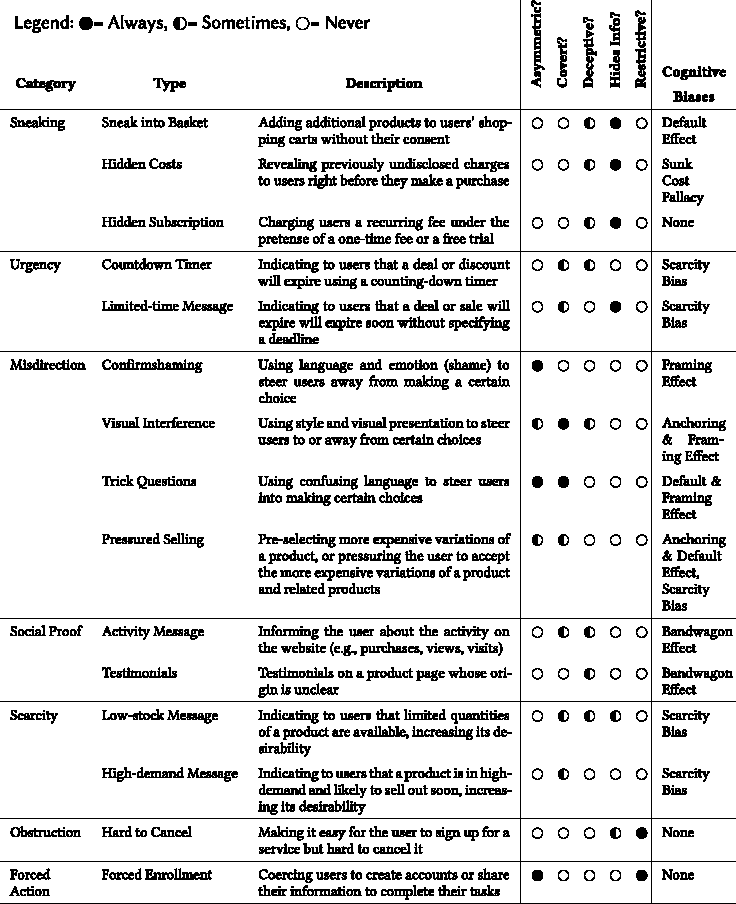
\includegraphics[width=1\textwidth]{media/dp-table.pdf}
\end{table}
\chapter{Machine Learning}

The term machine learning was firstly coined in 1959 by Arthur Samuel. He described machine learning as: "the field of study that gives computers the ability to learn without being explicitly programmed."\cite{machine-learning-samuel}.

Tom M. Mitchell proposed a new formal definition in 1997\cite{machine-learning-mitchell}, which is:
\begin{definition}
A computer program is said to learn from experience $E$ with respect to some class of tasks $T$ and performance measure $P$, if its performance at tasks in $T$, as measured by $P$, improves with experience $E$.
\end{definition} 

Mitchell also describes an example where a computer program that learns to play chess improves its performance $P$ by gaining experience $E$ from games played against itself. Performance $P$ is measured as the ability to win in a class of tasks $T$, which in this example are the tasks of playing checkers.

\subsection*{A checkers learning problem:}

\begin{itemize}
    \item Task $T$: playing checkers
    \item Performace measure $P$: percent of games won againts humans or other programs
    \item Training experience $E$: percent of games won againts itself
\end{itemize}


Mitchell continues that all learning problems can be specified in this way, such as learning to recognise handwritten words, or learning to drive a robotic automobile autonomously.

\subsection*{A handwritten recognition learning problem:}

\begin{itemize}
    \item Task $T$: recognising and classifying handwritten words in a picture
    \item Performace measure $P$: percent of correctly recognised words
    \item Training experience $E$: a dataset of handwritten words with correct recognition
\end{itemize}

\subsection*{A robot driving learning problem:}

\begin{itemize}
    \item Task $T$: driving on a highway using cameras
    \item Performace measure $P$: average distance travelled before an error occurs
    \item Training experience $E$: a recorded video of a human driver as a sequence of images and steering commands
\end{itemize}

\section{Approaches}

Traditionally, all machine learning tasks can be divided into three broad categories according to the type of feedback provided to the learning system. These are supervised learning, unsupervised learning, and reinforcement learning\cite{ml-types1,ml-types2}.

Reinforcement learning is not described at all in this thesis, as reinforcement learning is not suitable for any type of machine learning problem addressed in the practical part of the thesis.

\begin{figure}[ht]
    \centering
    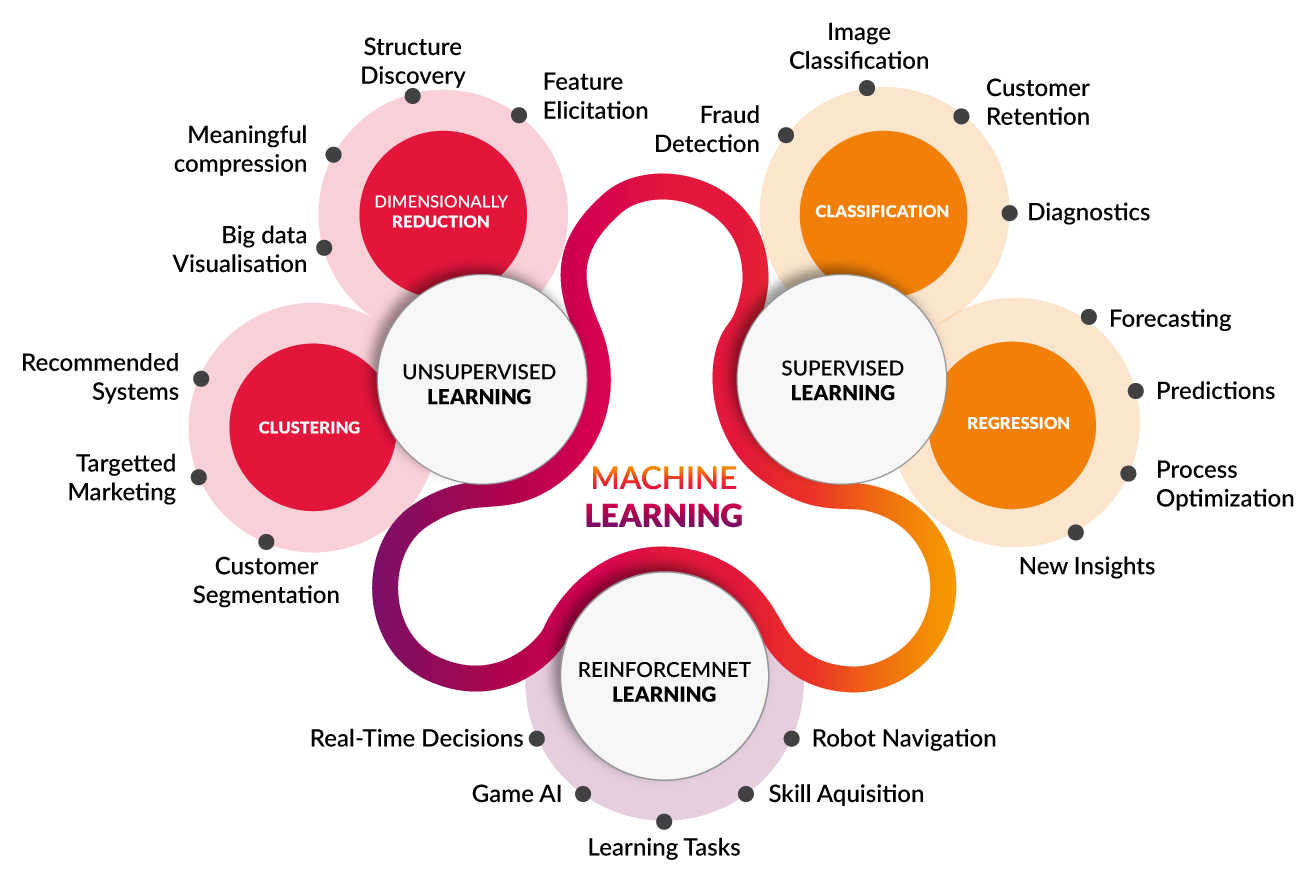
\includegraphics[width=1\linewidth]{media/machine-learning-approaches.png}
    \caption{The three basic learning approaches in machine learning with subcategories and typical applications. The vast majority of machine learning algorithms fall into these three categories.\cite{machine-learning-approaches}}
    \label{fig:machine-learning-approaches}
\end{figure}

Some literature\cite{ml-types1,ml-types2} defines semi-supervised learning, which combines supervised and unsupervised approaches mentioned above, as another learning method. However, since all three basic approaches can be combined, these combinations of learning approaches are omitted in this thesis.

It is also important to mention that the output of a machine learning algorithm, which is usually stored after the learning process and which is subsequently used in the decision-making process, is called a \textbf{model}\cite{algorithms-vs-models}.

\subsection{Supervised learning}

% přidat odkaz na kapitolu logistic regression

In supervised learning, the program is given a dataset that already contains not only what are the input variables, but also what the correct output should look like. Most times, this dataset is created by a person who knows what the correct output should be - a supervisor. Therefore, this type of learning is called as supervised learning.\cite{all-models}

Supervised learning problems are further categorized into two subcategories, classification and regression problems, depending on what the output is\cite{coursera-ml}. If the output is to be a numerical value, such as the price of a property, it is a regression problem. However, if the output is to be whether or not there is a cat in the picture, then it is classification problem. Also, it can be said that algorithms for regression problems are used to predict continues values and algorithms for classification problems are used to predict (or classify) discrete values.

\subsubsection{Regression}
As mentioned earlier, the output of regression algorithms is continuous values. It can be said that a regression solving algorithm looks for a correlation between the input dependent and independent variables. In detail, the input of the learning algorithm is the first pairs of input dependent and independent variables. The algorithm first searches for the mapping function that best captures the unknown correlation in the learning phase. After that, when the algorithm is presented with data for which we do not know the output, the algorithm uses this learned function to predict the value.

A common example of a regression problem is that a machine learning algorithm predicts property prices based on a dataset of properties sold in the past. This dataset contains features such as a number of rooms, location, property condition, and more. It also contains the sale price. Thus, in the learning phase, the algorithm estimates which features lead to which price. Or rather, what is the correlation between the properties of a property and its selling price. Subsequently, this learned model is saved. Then the algorithm is switched to a mode where it no longer learns but returns the property's price depending on what data it is given.

\subsubsection{Classification}

As with regression, the classification algorithm tries to find the correlation between the dependent and independent variables. The learning and subsequent prediction (classification) also work similarly to regression. The output of classification is not a continuous value but a discrete value. 

For example, it can be a decision whether a cancer is malignant or benign. The number of discrete values can be more than one. Also, the output of the classification does not have to always be a logical true-false value for every classification problem. The classification might recognize whether there is a pig, a dog, or a loaf of bread, or even something more in a picture.

\begin{figure}[ht]
    \centering
    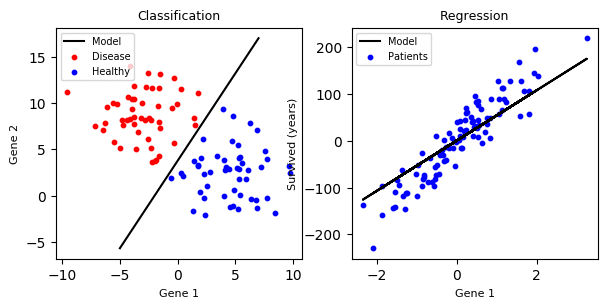
\includegraphics[width=1\linewidth]{media/classification-regression.png}
    \caption{Graph visualization of classification and regression tasks. Classification predicts which set a new patient fits into. Regression predicts the continuous value of the number of years a patient can survive.\cite{classification-regression}}
    \label{fig:classification-regression}
\end{figure}

\subsection{Unsupervised learning}
Unsupervised learning, unlike supervised learning, allows teaching a system without prior knowledge of what the output should look like. This type of learning looks for similarities and patterns in the data instead of mapping input values to labels in the dataset.\cite{coursera-ml}

Unsupervised learning is further divided into two subcategories based on how these similarities and patterns found in the data are used. These subcategories are clustering and dimensional reduction.

\subsubsection{Clustering}

% přidat odkaz na kapitolu HDBSCAN

The goal of clustering is to divide data that are similar into groups\cite{ml-types2}. The number of these groups can be an exact number defined by an expert for some algorithms (K-means\cite{k-means}), but there are also algorithms that find the number of groups by themselves (OPTICS\cite{optics}, DBSCAN\cite{dbscan}.

An example of using clustering methods is recommender systems that recommend the same things to users with similar characteristics to other users. Other examples include anomaly detection, statistical data analysis, and social network analysis\cite{clustering-applications}.

Clustering methods are broadly divided into \textbf{hard clustering} and \textbf{soft clustering}, depending on whether individual data points can fall into only one class (hard clustering) or multiple classes (soft clustering). In the case of soft clustering, each data point is scored with a probability measure that determines which clusters the data point belongs to \cite{clustering-types}. 

\textbf{Types of clustering methods:}
\begin{itemize}
    \item Partitioning Clustering
    \item Density-Based Clustering
    \item Hierarchical Clustering
    \item Grid-Based Clustering
    \item Fuzzy Clustering
\end{itemize}

It is not important for this thesis to describe all these types of clustering methods, except the HDBSCAN method (Hierarchical Density-Based Spatial Clustering of Applications with Noise) used in this thesis's practical part. HDBSCAN is a combination of Density-Based Clustering and Hierarchical Clustering. A detailed description and information about the HDBSCAN method are given in Section XY.

\subsubsection{Dimensional reduction}

% TODO - přidat odkaz na kapitolu PCA

As mentioned earlier, the main task of dimension reduction algorithms is to transform data from a higher dimensional space to a lower-dimensional space\cite{ml-types2}. This is often done during the preprocessing phase of the data, which can be sparse and contain much redundancy. Dimensional reduction algorithms select the interesting parts of the data in the dataset. This also avoids the problem of the curse of dimensionality\cite{bellman1957dynamic}.

Most dimensionality reduction algorithms are further divided into \textbf{feature extraction} or \textbf{feature elimination} algorithms\cite{ml-types2}.

A very commonly used dimensionality reduction algorithm is Principal component analysis, which is also used in the practical part of this thesis and is described in Chapter XX.

\begin{figure}[ht]
    \centering
    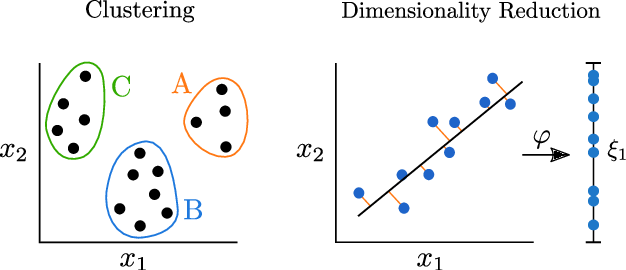
\includegraphics[width=1\linewidth]{media/clustering-reduction.png}
    \caption{Illustration of the output of clustering and dimensional reduction. Clustering searches for patterns among distantly similar data. Dimensional reduction transforms higher dimensional data into lower dimensional data.\cite{clustering-reduction}}
    \label{fig:clustering-reduction}
\end{figure}


% \input{"chapters/04-setup.tex"}
\chapter{Corpus Creation}

One of the steps of the analysis of the prevalence of the dark pattern on Czech webshops is to find webshops URLs on a large scale autonomously. The Princeton researchers used Alexa Rank\cite{alexa-topsites} made by a web traffic analysis company, Alexa Internet. Alexa Rank is a measure of website popularity. Alexa Internet provides API to fetch a list of most popular websites by Alexa Rank. However, this list contains other types of websites as well, not only webshops that researchers focus on. Also, non-English websites are included as well. Because of that, researchers implemented a couple of mechanisms to cherry-pick English webshops only, discussed earlier in the state-of-the-art chapter of this thesis.

As said before, this thesis aims to analyse Czech webshops and because of that, using Alexa Rank is not efficient enough. Alexa API provides only the first five hundred thousand most popular websites, which is a reason why it contains a small number of Czech websites and even fewer Czech webshops. However, the Czech Internet (that means only websites in the Czech language) is relatively small compared to the English Internet. Also, the English Internet is under multiple jurisdictions, but the Czech Internet is not. Therefore, the Czech Internet is more consistent, and a result of it is that this environment allows creating companies that make Internet catalogues and comparison shopping websites (aggregators) that cover a significant portion of the Czech Internet. 

These catalogues and tools also sometimes rank the listed websites by a measure that has connotations to popularity. For example, a number of testimonials are an excellent resource that reflects the popularity of the webshop. These catalogues and aggregators can be used to mine the URLs of Czech webshops from them instead of using Alexa Rank API. Also, if there is a similar measure as described above, the analysis results can be compared to Princeton's researcher analysis, revealing a correlation of dark patterns evidence on the website and the popularity of the website.

While searching the Internet, several such suitable sites were discovered that contain extensive lists of Czech webshops. Examples of the most suitable sites are Heureka.cz, Asociaceeshopu.cz and Shopy.cz.

Other vital facts that played a role and were considered in the selection of the only one website (that is later used for the creation of the list of Czech webshops) were the actual cover of the Czech Internet. Heureka has by far the highest number of webshops in their listings\cite{srovnavace-shoptet}. However, a few of the biggest webshops do not want to be listed on Heureka. Their reason is usually Heureka itself because it compares the prices of products on the enlisted webshops. Also, Heureka is a part of a business group that runs several competitive webshops. Because of that, the final list (made in this practical part of the study) of Czech webshops was manually checked if it contains the five biggest webshops (according to the list published on website peak.cz\cite{peak-eshopy}), and it does.

\begin{figure}[ht]
    \centering
    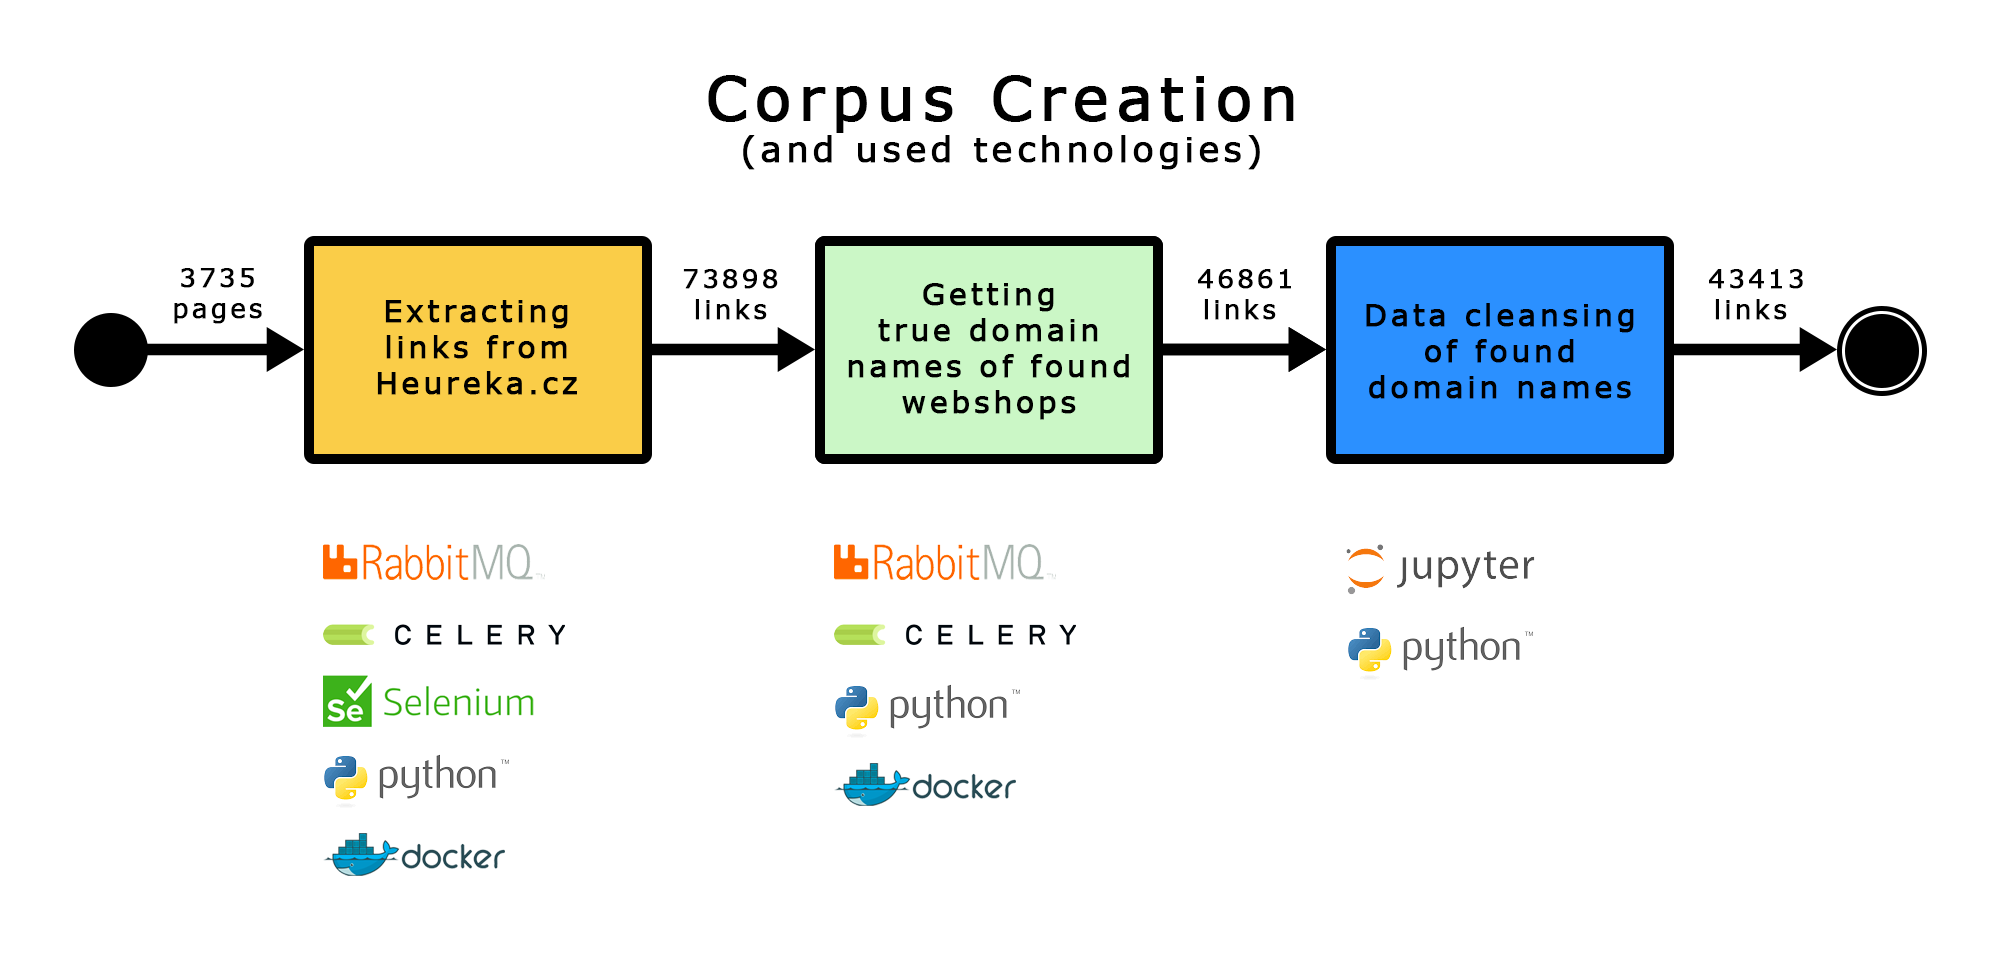
\includegraphics[width=1\linewidth]{media/corpus_creation.png}
    \caption{All steps of corpus creation, which starts with a list of webshops available on Heureka.cz, paginated into 3735 pages and ends with a list of 43413 unique webshops' URLs in CSV format.}
    \label{fig:corpus_creation}
\end{figure}

\section{Extracting webshops from Heureka}

Heureka provides a list of all registered webshops on their website. This list is paginated, where every page contains twenty records of webshops. However, Heureka does not provide the total number of these pages. 

In February 2021, the total number of pages was 3735. This number of pages was manually found by changing the query parameters from the URL until the page stopped returning error 404. At the same time, these 3735 pages contained 74698 webshops in total. 

A web crawler was made to extract webshops' links and names from these pages. The crawler is written in Python 3, using Selenium framework with Chrome browser in headless mode. Also, the crawler is parallelised to speed up this task using Celery asynchronous task queue. Source codes are inside \textbf{src\string/crawler\string/extract\_shops} folder. 

Some of the crawled pages were not successfully downloaded because the Chrome browser occasionally failed to start or the webserver returned an empty page. The crawler was still able to successfully download \textbf{3695 pages} containing \textbf{73898 webshops} in total after scraping the HTML into 3695 CSV files.

Such a high number of obtained webshops does not correspond with the number of webshops that Heureka claims to contain on its homepage (it claims to aggregate around 38000 webshops). Also, the estimated number of webshops on the Czech Internet is around 41000 according to a study made by Zbozi.cz and Shoptet.cz\cite{srovnavace-shoptet}. The cause of this is that the retrieved list of webshops contains many duplicities and already inactive webshops.

Another problem with this list is that the retrieved links are not the actual domain names of the webshops. These URLs are redirections, and they must be visited first to retrieve the actual domain name.

The two other steps of the Corpus Creation deal with these two problems.

\section{Retrieving true domain names}

As mentioned above, Heureka does not provide direct URLs to webshops in its listings. The provided links only redirect to the true URLs of webshops, and because of that, another crawler was made to follow these redirections and return the true URLs. This crawler is also written in Python 3. This time, the task is only to retrieve the true URLs. Hence, Request library is used instead of Selenium, which is too complex for such a simple task. It remains parallelized using Celery. Sources codes are in \textbf{src\string/crawler\string/reveal\_true\_domains} folder.

This crawler adds an additional column to the dataset given from the previous crawler, which contains the true URL. If an exception occurred during the execution of the single task, its message is written there instead. If the webpage returned a different status code than 200, the status code is also written there instead. The importance of this data about errors and exceptions are helpful in the validation of the whole task. Whether the whole task is successful or it returns too many errors and exceptions.

\section{Cleansing of dataset}

The given data from the previous crawler is further cleansed in a Jupyter notebook \textbf{src\string/crawler\string/domain\_dataset\_cleansing.ipynb} using primarily Pandas library.

In the first step, the dataset is split into two data frames of errors and true URLs. Dataset of errors contains 27037 rows, and 23238 of them are results of connection being refused after redirection. The first exception might be that Heureka implemented mechanisms to prevent the crawling of the redirections. This claim was refuted by \textbf{manually going through 100 random} links. None of these links redirects to an active webshop. The next most frequent errors were 404 errors with 1953 occurrences, 403 errors with 750 occurrences and 503 errors with 504 occurrences. These are errors that indicate that the web store web page is no longer active. The other errors had an incidence of fewer than 200 occurrences.

The dataset of true URLs is further cleansed by filtering out other identified inactive webshops that were not identified in the error/rejection filtering. Firstly, such webshops URLs have a high frequency in the dataset because the webshops' URLs are often redirected to the webshops' hosting service website after deactivation of the webshop. For example, many Czech webshops use Shoptet service, which allows users to rent a done webshop solution for a monthly payment. After the users stop paying this fee, their webshop is inactivated (or deleted), making the original webshop be redirected to Shoptet's custom webpage informing visitors about the inactivation of the particular webshop. Secondly, many URLs of inactive webshops contain status code in the URL without sending the actual status code in an HTTP response. Lastly, some domain names were inactive or resold and redirected to a new website (surprisingly redirected to porn websites in most of the cases). All this manual work led to creating a list of such URLs and was used to filter them out of the dataset. This shrinked the dataset from \textbf{46861} to \textbf{46023} rows, removing another \textbf{838} rows.

The last step is to remove URI parts from the URLs and drop duplicate entries, which shrank the dataset to final \textbf{43413} unique links to webshops, removing another \textbf{2610} rows.

Links to download all the outputs and logfiles of crawling are on README page of GitHub repository of this thesis. The link to this repository is in Appendix B (Supplemental Material) of this thesis.

The final list of Corpus Creation stage can be found \textbf{clean\_eshop\_list.csv} in an archive \textbf{reveal\_true\_domains\_crawl\_2021\_02\_23.tar.bz2}.

% dát tam tabulčičku, která to zesumíruje
\chapter{Data Collection}

The second step of the analysis is to find the candidates for dark patterns. This thesis, like the paper on which it is based\cite{dark-patterns-at-scale}, focuses only on a textual representation of dark patterns in terms of finding candidates.

A random sample of one hundred records was drawn from the final dataset from the previous chapter. The URLs from this sample were manually visited, and it was found that the linked page was not a web store for six samples, and thirteen were already non-functional URLs. In addition, it was discovered that the more of these non-compliant URLs mainly were located at lower positions in the dataset. This finding is not surprising, as large web stores last longer and thus are higher in the list of stores.

This sample is updates and user later in data colletion, where records with non-compliant URL are replaced with compliant ones for a total of one hundred records. This sample is saved in \textbf{src/crawlers/extract\_links/list-100-shops.csv}

Looking for the candidates is divided in two steps or two crawlers respectively. The goal of the first step is to find product pages on the webshops in the final list from the chapter Corpus Creation. The goal of the second step is to lookup for the textual candidates on the found product pages and saving them into Redis database for the further analysis.

The two crawlers are based on the crawlers implemented for the original research done at Princeton\cite{dark-patterns-at-scale}. The original crawlers are written in Python 2 and now rewritten into Python 3, since the Python 2 is a deprecated version since January 2020. These crawlers are build in Selenium framework and they use Javascript for the navigation in DOM structure of websites









% Náhodně jsem vybral 100 linků z nichž 6 nebylo eshopem, 13 bylo již nefunkčních. Pravděpodobně čím níže link je, tím menší pravděpodobnost, že bude fungovat. Abych to mohl potvrdit, tak by bylo třeba otestovat více odkazů. Tento list jsem doplnit o nové eshopy, které jsem taktéž ověřil, zda se jedná o eshopy.

% Update:
% Aktualizoval jsem program tak, aby fungoval v Pythonu3.
% Zároveň jsem přidal možnost vyhledávat bez predikce. To jsem dělal kvůli tomu, abych mohl vyhledat seznam linků, které poté určím, že jsou produktové stránky. Nicméně systém nefungoval tak jak jsem myslel a procházel zbytečně moc webových stránek, které evidentně nebyly produktové.
% Program jsem upravil také tak, že jsem přidal různé české varianty a překlady slov a používáných frází, které jsou programem použity na vyhledávání akčních tlačítek jako "Vložit do košíku" a také na filtraci stránek, které zřejmě nejsou produktové (kontakty, o nás, košík atp.)

% Provedl jsem krátný průzkum nejčastěji používaných frází pro vkládání do košíku. Provedl jsem tedy manuální procházení produktových stránek ze seznamu 50 stránek a našel tyto nejčastější fráze:
% 1) Do košíku (19 z 50)
% 2) Přidat do košíku (18 z 50)
% 3) Koupit (7 z 50)
% 4) Vložit do košíku (6 z 50)

% Z tohoto vyplývá, že jediné použité fráze jsou "do košíku" a "koupit". S vyznamností se neobjevují odchylky ve skloňování atp.

% Přidat pak info o tom, na cem to bezelo, jak rychle atp.



% Únor 2021

% Získávání kandidátů na Dark Patterns z produktových stránek:
% - Pro hledání produktových stránek je vytvořený spider, který prochází adresy na doméně a rozpoznává z těchto adres, které adresy jsou produktových stránek. Rozpoznání produktové stránky zajištuje naučený klasifikátor na rozpoznávání produktových stránek.

%     Učení modelu pro klasifikaci produktové stránky:
%     - Tento klasifikátor je naučený v Jupyter notebooku ProductPageClassifier.ipynb. Adresy, které jsou využity pro učení klasifikátoru jsou získány přes jednoduchý spider z náhodných domén v datasetu. Ručně jsou tyto získané adresy ohodnoceny, zda se jedná o produktovou stránku, či nikoliv. 

%     Procházení produktových stránek:
%     - 
\chapter{Data Analysis}
    Analyzing millions of segments is not optimal for an expert analyst. The work of this expert is expensive and time-consuming. Therefore, methods that reduce the number of segments and thus the expert's work need to be used to make the analysis manageable for the expert. The output is a list of text segments that contain dark patterns.

    The methods used in this section follow the work of the Princeton researchers. At the same time, the results of this work are again compared with the results of their work.

    The data analysis can be divided into four steps:

    \section{Preprocessing}
        The SQLite database, which has 9.5 million segments, contains many duplicate segments across multiple websites. For example, "Add to Cart" buttons, various unified headings such as "Product Description", and others. Since only the text of the segments is analyzed, only those segments that have unique text across a single domain are selected from the dataset for further processing. Also, all the numbers in the dataset have been replaced with placeholders, thus reducing the dataset even more. 

        The output of this preprocessing is a reduction in the number of segments from ~9.5M segments to ~805K. Thus, this approach led to a 92\% reduction in the number of segments. Again, the results are similar to those of the Princeton researchers who achieved a 90\% reduction.

    \section{Feature processing}
        In order to be able to use clustering in the next step, the texts of the segments must first be transformed into a representation for which the similarities between the segments can be expressed mathematically (hereafter, the document means the internal text of the segment).  For this purpose, the Bag-of-Words model is used here. This model is a type of word embedding that represents a document as a string of the number of occurrences of words from a dictionary of all words used across all documents. 

        However, many words do not have only one base form. Especially in the English language, a single word can have many forms due to inflections such as declension and conjugation. The basis of the Bag-of-Words model is the previously mentioned dictionary. If that dictionary contained all the occurrences of the different forms of words, the dictionary would be unnecessarily large and inefficient. For example, the distances of two very similar documents could be disproportionately large simply by rewriting them in a different tense.

        This mischief can be avoided by stemming or lemmatisation, where stemming returns the roots of words. Lemmatization produces the basic forms of words (infinitive for verbs and first-person singular for nouns, adjectives, pronouns and numerals). Lemmatization also considers the context of the word and is, therefore, more accurate\cite{stemming-and-lemmatisation}. On the other hand, it is slower than stemming.

        The Princeton researchers used stemming from the NLTK Python library\cite{nltk}. Still, because both methods (stemming and lemmatisation) depend on the language and because the NLTK library does not support the Czech language, another library had to be chosen.

        Such a library is UDPipe\cite{udpipe} by the Institute of Formal and Applied Linguistics at Charles University. Also, one of the functionalities of this library is tokenisation in the Czech language, which is needed to split the documents into individual words (also referred to as tokens)\cite{tokenisation}.

        Each document is tokenised during the dictionary creation process, producing a list of tokens for which lemmas are obtained and then added to the dictionary. Also, stop words from the Czech language and punction are filtered out of these lists.

        The vocabulary after all the described steps above had a size of \textbf{~269K} tokens. However, this vocabulary still contained tokens, which did have not enough occurrences in the documents.

        Furthermore, only those that appeared in the documents at least 100 times were selected. There were only 188 such tokens. The Count Vectorizer\cite{count-vectorizer} was used to create the BoW matrix, which counts the number of token occurrences in a document. 

        Using Principal Component Analysis (PCA) with 3 retained components on the BoW matrix led to a dimensional reduction which captured 95\% of the variance in the data.

    \section{Clustering}
        The goal of clustering is to group data together. In this case, it means clustering segments into clusters based on similarity. The expert then evaluates the resulting clusters, which makes the expert's job of manual passes easier.

        The clustering method used was HDBSCAN (Hierarchical Density-based Spatial Clustering of Applications with Noise). According to the Princeton researchers, they selected this clustering algorithm because it is robust to noise and, in particular, allows to choose the minimum size of the output clusters.

        In total, HDBSCAN was performed for four different hyperparameter settings. The number of output clusters and the size of the noise cluster was analysed.  The metric used and the minimum cluster size mentioned earlier were the hyperparameters varied. The metrics used were $L_{1}$ and $L_{2}$ norms, also known as Manhattan and Euclidean distance. The hyperparameter of the minimum cluster sizes selected was 5 and 10 segments, which keep the size of noise small and prevents two or more clusters (that are separatable) from forming only one.

        The analysis showed the number of clusters is significantly lower for the models with a minimum cluster size of 10 segments. Similarly, as for the results from Princeton researchers, the difference between selected metric distances was not very significant for data. As expected, models with a larger minimum cluster size have a larger noise cluster size. However, this noise cluster is slightly less than 50\% larger, while the number of all clusters is twice as small. Therefore, a model with a minimum cluster size of 5 segments was selected using the Manhattan distance as the metric with \textbf{4248} clusters (one cluster is the noise cluster). The table \ref{table:hyperparameters-hdbscan} summarised the number of clusters and size of noise for the given hyperparameters. 

        \begin{table}[h!]
            \centering
            \begin{tabular}{r|cr|cr|}
            Minimum cluster size  & \multicolumn{2}{c|}{5}                               & \multicolumn{2}{c|}{10}                              \\ \hline
            Distance metric       & \multicolumn{1}{c|}{L1}    & \multicolumn{1}{c|}{L2} & \multicolumn{1}{c|}{L1}    & \multicolumn{1}{c|}{L2} \\ \hline
            Number of clusters    & \multicolumn{1}{r|}{9040}  & 9088                    & \multicolumn{1}{r|}{4249}  & 4265                    \\ \hline
            Size of noise cluster & \multicolumn{1}{r|}{80980} & 80083                   & \multicolumn{1}{r|}{98436} & 97651                   \\ \cline{1-5} 
            \end{tabular}
            \caption{Number of clusters and size of noise cluster for different distance metrics and minimum size of a cluster.}
            \label{table:hyperparameters-hdbscan}
        \end{table}

    \section{Analysis of output clusters}
    \label{section:analysis-of-output-clusters}
        The clusters that were obtained in the previous step are manually scanned in two steps.

        In both passes, I put myself in the role of an expert who evaluates what is and what is not a dark pattern. I used the knowledge I gained from writing the Dark patterns section. I also used available literature \cite{dark-patterns-brignull-types}\cite{dark-patterns-colin}\cite{kysar-douglas}\cite{taxonomies-tales}\cite{taxonomies-conti}. In uncertainty, I also used the Internet to find out examples what is and what is not a dark pattern, to keep my decisions even more objective. However, the subjective component could still play a role in the decision making process.

        In the first pass, I selected those clusters for which any segment could manifest a dark pattern. For example, the selected clusters were commonly countdowns, total cart prices, user references, notifications, product options, logins and registrations. Only the text components of the segments were checked, not how the segment actually looks on the page. This pass resulted in the number of clusters being reduced from 4249 to 477.
        
        In pass two, I investigate these 477 clusters by directly visiting the website where the dark pattern is searched. If the page no longer exists or does not match the segment, then I investigated screenshots that were obtained during the simulated putchase flow instead. I extended this search by manually going through the entire shopping process directly on the web page and manually searching for all dark patterns.
        
        Lastly, this output dataset of found dark patterns is examined and cleaned from duplicities.
\chapter{Evaluation}

At first, it is imporant to note the limitations of the analysis and the evaluation.

\section{Limitations}
As mentioned in the previous chapter, deciding what is still a harmless user inferface pattern and what is already a dark pattern is a complex task. It always depends on the subjective opinion of the expert. At the same time, different types of dark patterns affect each customer differently. To make the analysis to be more objective, several steps were done as described earlier in \nameref{section:section:analysis-of-output-clusters}. Also, more experts analysing the clusters would lead only to a more objective results.

Another limitation of this work is that it considers only the textual segments on the page and ignores the appearance of these segments. Thus, it cannot find dark patterns in images, for example.

During the analysis, it was also found that some webshops use dark patterns to increase their number of references on Heureka.cz. This behaviour could significantly affect their position in the overall ranking, especially for the lower-ranked webshops, where a small number of references can make a significant change in the rank.

Lastly, not every webpage was a part of the analysis due to simulation of the checkout flow only. Homepage, listings of products, registration page, login page, and payment page were omitted in the flow.


\begin{table}[h!]
    \centering
    \bgroup
    \def\arraystretch{1.65}
        \begin{tabular}{ll|l}
            \toprule
            \textbf{Category}                     & \textbf{Type}                      & \textbf{\# Instances}                     \\ \hline
            Sneaking                              & Sneak into Basket                  & 2                                         \\
                                                  & Hidden Costs                       & 0                                         \\
                                                  & Hidden Subscription                & 0                                         \\ \hline
            Urgency                               & Countdown Timer                    & 23                                        \\
                                                  & Limited-time Message               & 17                                        \\ \hline
            Misdirection                          & Confirmshaming                     & 0                                         \\
                                                  & Visual Interference                & 28                                        \\
                                                  & Trick Questions                    & 68                                        \\
                                                  & Pressured Selling                  & 924                                       \\ \hline
            Social Proof                          & Activity Message                   & 223                                       \\
                                                  & Testimonials                       & 19                                        \\ \hline
            Scarcity                              & Low-stock Message                  & 38                                        \\
                                                  & High-demand Message                & 7                                         \\ \hline
            Obstruction                           & Hard to Cancel                     & 6                                         \\ \hline
            Forced Action                         & Forced Enrollment                  & 75                                        \\ \hline                                       
            \end{tabular}
        \egroup
    \caption{Number of Dark patterns instances found on Czech webshops, divided into categories and types.}
    \label{table:summary-dark-patterns}
\end{table}

\section{Webshops using Dark patterns prevelance}

A total number of 1419 dark patterns were found on 1081 webshops from a total of 10K webshops, which makes 10.81\% of all webshops to contains at least one instance of Dark Pattern. No dark patterns of the Hidden Costs, Corfirmshaming and Hidden Subscription types were found during the manual passes. The found instances of Dark Pattern are divided into categories and types showed in table \ref{table:summary-dark-patterns}.

\begin{figure}
    \begin{center}
        %% Creator: Matplotlib, PGF backend
%%
%% To include the figure in your LaTeX document, write
%%   \input{<filename>.pgf}
%%
%% Make sure the required packages are loaded in your preamble
%%   \usepackage{pgf}
%%
%% and, on pdftex
%%   \usepackage[utf8]{inputenc}\DeclareUnicodeCharacter{2212}{-}
%%
%% or, on luatex and xetex
%%   \usepackage{unicode-math}
%%
%% Figures using additional raster images can only be included by \input if
%% they are in the same directory as the main LaTeX file. For loading figures
%% from other directories you can use the `import` package
%%   \usepackage{import}
%%
%% and then include the figures with
%%   \import{<path to file>}{<filename>.pgf}
%%
%% Matplotlib used the following preamble
%%   \usepackage{fontspec}
%%   \setmainfont{DejaVuSerif.ttf}[Path=/Users/petrhanzl/anaconda3/lib/python3.8/site-packages/matplotlib/mpl-data/fonts/ttf/]
%%   \setsansfont{DejaVuSans.ttf}[Path=/Users/petrhanzl/anaconda3/lib/python3.8/site-packages/matplotlib/mpl-data/fonts/ttf/]
%%   \setmonofont{DejaVuSansMono.ttf}[Path=/Users/petrhanzl/anaconda3/lib/python3.8/site-packages/matplotlib/mpl-data/fonts/ttf/]
%%
\begingroup%
\makeatletter%
\begin{pgfpicture}%
\pgfpathrectangle{\pgfpointorigin}{\pgfqpoint{5.000000in}{2.000000in}}%
\pgfusepath{use as bounding box, clip}%
\begin{pgfscope}%
\pgfsetbuttcap%
\pgfsetmiterjoin%
\definecolor{currentfill}{rgb}{1.000000,1.000000,1.000000}%
\pgfsetfillcolor{currentfill}%
\pgfsetlinewidth{0.000000pt}%
\definecolor{currentstroke}{rgb}{1.000000,1.000000,1.000000}%
\pgfsetstrokecolor{currentstroke}%
\pgfsetdash{}{0pt}%
\pgfpathmoveto{\pgfqpoint{0.000000in}{0.000000in}}%
\pgfpathlineto{\pgfqpoint{5.000000in}{0.000000in}}%
\pgfpathlineto{\pgfqpoint{5.000000in}{2.000000in}}%
\pgfpathlineto{\pgfqpoint{0.000000in}{2.000000in}}%
\pgfpathclose%
\pgfusepath{fill}%
\end{pgfscope}%
\begin{pgfscope}%
\pgfsetbuttcap%
\pgfsetmiterjoin%
\definecolor{currentfill}{rgb}{1.000000,1.000000,1.000000}%
\pgfsetfillcolor{currentfill}%
\pgfsetlinewidth{0.000000pt}%
\definecolor{currentstroke}{rgb}{0.000000,0.000000,0.000000}%
\pgfsetstrokecolor{currentstroke}%
\pgfsetstrokeopacity{0.000000}%
\pgfsetdash{}{0pt}%
\pgfpathmoveto{\pgfqpoint{0.625000in}{0.250000in}}%
\pgfpathlineto{\pgfqpoint{4.500000in}{0.250000in}}%
\pgfpathlineto{\pgfqpoint{4.500000in}{1.760000in}}%
\pgfpathlineto{\pgfqpoint{0.625000in}{1.760000in}}%
\pgfpathclose%
\pgfusepath{fill}%
\end{pgfscope}%
\begin{pgfscope}%
\pgfpathrectangle{\pgfqpoint{0.625000in}{0.250000in}}{\pgfqpoint{3.875000in}{1.510000in}}%
\pgfusepath{clip}%
\pgfsetbuttcap%
\pgfsetmiterjoin%
\definecolor{currentfill}{rgb}{0.415686,0.678431,0.894118}%
\pgfsetfillcolor{currentfill}%
\pgfsetlinewidth{1.405250pt}%
\definecolor{currentstroke}{rgb}{0.000000,0.396078,0.741176}%
\pgfsetstrokecolor{currentstroke}%
\pgfsetdash{}{0pt}%
\pgfpathmoveto{\pgfqpoint{0.801136in}{0.250000in}}%
\pgfpathlineto{\pgfqpoint{0.871591in}{0.250000in}}%
\pgfpathlineto{\pgfqpoint{0.871591in}{1.112857in}}%
\pgfpathlineto{\pgfqpoint{0.801136in}{1.112857in}}%
\pgfpathclose%
\pgfusepath{stroke,fill}%
\end{pgfscope}%
\begin{pgfscope}%
\pgfpathrectangle{\pgfqpoint{0.625000in}{0.250000in}}{\pgfqpoint{3.875000in}{1.510000in}}%
\pgfusepath{clip}%
\pgfsetbuttcap%
\pgfsetmiterjoin%
\definecolor{currentfill}{rgb}{0.415686,0.678431,0.894118}%
\pgfsetfillcolor{currentfill}%
\pgfsetlinewidth{1.405250pt}%
\definecolor{currentstroke}{rgb}{0.000000,0.396078,0.741176}%
\pgfsetstrokecolor{currentstroke}%
\pgfsetdash{}{0pt}%
\pgfpathmoveto{\pgfqpoint{0.871591in}{0.250000in}}%
\pgfpathlineto{\pgfqpoint{0.942045in}{0.250000in}}%
\pgfpathlineto{\pgfqpoint{0.942045in}{0.861190in}}%
\pgfpathlineto{\pgfqpoint{0.871591in}{0.861190in}}%
\pgfpathclose%
\pgfusepath{stroke,fill}%
\end{pgfscope}%
\begin{pgfscope}%
\pgfpathrectangle{\pgfqpoint{0.625000in}{0.250000in}}{\pgfqpoint{3.875000in}{1.510000in}}%
\pgfusepath{clip}%
\pgfsetbuttcap%
\pgfsetmiterjoin%
\definecolor{currentfill}{rgb}{0.415686,0.678431,0.894118}%
\pgfsetfillcolor{currentfill}%
\pgfsetlinewidth{1.405250pt}%
\definecolor{currentstroke}{rgb}{0.000000,0.396078,0.741176}%
\pgfsetstrokecolor{currentstroke}%
\pgfsetdash{}{0pt}%
\pgfpathmoveto{\pgfqpoint{0.942045in}{0.250000in}}%
\pgfpathlineto{\pgfqpoint{1.012500in}{0.250000in}}%
\pgfpathlineto{\pgfqpoint{1.012500in}{1.184762in}}%
\pgfpathlineto{\pgfqpoint{0.942045in}{1.184762in}}%
\pgfpathclose%
\pgfusepath{stroke,fill}%
\end{pgfscope}%
\begin{pgfscope}%
\pgfpathrectangle{\pgfqpoint{0.625000in}{0.250000in}}{\pgfqpoint{3.875000in}{1.510000in}}%
\pgfusepath{clip}%
\pgfsetbuttcap%
\pgfsetmiterjoin%
\definecolor{currentfill}{rgb}{0.415686,0.678431,0.894118}%
\pgfsetfillcolor{currentfill}%
\pgfsetlinewidth{1.405250pt}%
\definecolor{currentstroke}{rgb}{0.000000,0.396078,0.741176}%
\pgfsetstrokecolor{currentstroke}%
\pgfsetdash{}{0pt}%
\pgfpathmoveto{\pgfqpoint{1.012500in}{0.250000in}}%
\pgfpathlineto{\pgfqpoint{1.082955in}{0.250000in}}%
\pgfpathlineto{\pgfqpoint{1.082955in}{1.076905in}}%
\pgfpathlineto{\pgfqpoint{1.012500in}{1.076905in}}%
\pgfpathclose%
\pgfusepath{stroke,fill}%
\end{pgfscope}%
\begin{pgfscope}%
\pgfpathrectangle{\pgfqpoint{0.625000in}{0.250000in}}{\pgfqpoint{3.875000in}{1.510000in}}%
\pgfusepath{clip}%
\pgfsetbuttcap%
\pgfsetmiterjoin%
\definecolor{currentfill}{rgb}{0.415686,0.678431,0.894118}%
\pgfsetfillcolor{currentfill}%
\pgfsetlinewidth{1.405250pt}%
\definecolor{currentstroke}{rgb}{0.000000,0.396078,0.741176}%
\pgfsetstrokecolor{currentstroke}%
\pgfsetdash{}{0pt}%
\pgfpathmoveto{\pgfqpoint{1.082955in}{0.250000in}}%
\pgfpathlineto{\pgfqpoint{1.153409in}{0.250000in}}%
\pgfpathlineto{\pgfqpoint{1.153409in}{1.220714in}}%
\pgfpathlineto{\pgfqpoint{1.082955in}{1.220714in}}%
\pgfpathclose%
\pgfusepath{stroke,fill}%
\end{pgfscope}%
\begin{pgfscope}%
\pgfpathrectangle{\pgfqpoint{0.625000in}{0.250000in}}{\pgfqpoint{3.875000in}{1.510000in}}%
\pgfusepath{clip}%
\pgfsetbuttcap%
\pgfsetmiterjoin%
\definecolor{currentfill}{rgb}{0.415686,0.678431,0.894118}%
\pgfsetfillcolor{currentfill}%
\pgfsetlinewidth{1.405250pt}%
\definecolor{currentstroke}{rgb}{0.000000,0.396078,0.741176}%
\pgfsetstrokecolor{currentstroke}%
\pgfsetdash{}{0pt}%
\pgfpathmoveto{\pgfqpoint{1.153409in}{0.250000in}}%
\pgfpathlineto{\pgfqpoint{1.223864in}{0.250000in}}%
\pgfpathlineto{\pgfqpoint{1.223864in}{0.789286in}}%
\pgfpathlineto{\pgfqpoint{1.153409in}{0.789286in}}%
\pgfpathclose%
\pgfusepath{stroke,fill}%
\end{pgfscope}%
\begin{pgfscope}%
\pgfpathrectangle{\pgfqpoint{0.625000in}{0.250000in}}{\pgfqpoint{3.875000in}{1.510000in}}%
\pgfusepath{clip}%
\pgfsetbuttcap%
\pgfsetmiterjoin%
\definecolor{currentfill}{rgb}{0.415686,0.678431,0.894118}%
\pgfsetfillcolor{currentfill}%
\pgfsetlinewidth{1.405250pt}%
\definecolor{currentstroke}{rgb}{0.000000,0.396078,0.741176}%
\pgfsetstrokecolor{currentstroke}%
\pgfsetdash{}{0pt}%
\pgfpathmoveto{\pgfqpoint{1.223864in}{0.250000in}}%
\pgfpathlineto{\pgfqpoint{1.294318in}{0.250000in}}%
\pgfpathlineto{\pgfqpoint{1.294318in}{1.436429in}}%
\pgfpathlineto{\pgfqpoint{1.223864in}{1.436429in}}%
\pgfpathclose%
\pgfusepath{stroke,fill}%
\end{pgfscope}%
\begin{pgfscope}%
\pgfpathrectangle{\pgfqpoint{0.625000in}{0.250000in}}{\pgfqpoint{3.875000in}{1.510000in}}%
\pgfusepath{clip}%
\pgfsetbuttcap%
\pgfsetmiterjoin%
\definecolor{currentfill}{rgb}{0.415686,0.678431,0.894118}%
\pgfsetfillcolor{currentfill}%
\pgfsetlinewidth{1.405250pt}%
\definecolor{currentstroke}{rgb}{0.000000,0.396078,0.741176}%
\pgfsetstrokecolor{currentstroke}%
\pgfsetdash{}{0pt}%
\pgfpathmoveto{\pgfqpoint{1.294318in}{0.250000in}}%
\pgfpathlineto{\pgfqpoint{1.364773in}{0.250000in}}%
\pgfpathlineto{\pgfqpoint{1.364773in}{1.220714in}}%
\pgfpathlineto{\pgfqpoint{1.294318in}{1.220714in}}%
\pgfpathclose%
\pgfusepath{stroke,fill}%
\end{pgfscope}%
\begin{pgfscope}%
\pgfpathrectangle{\pgfqpoint{0.625000in}{0.250000in}}{\pgfqpoint{3.875000in}{1.510000in}}%
\pgfusepath{clip}%
\pgfsetbuttcap%
\pgfsetmiterjoin%
\definecolor{currentfill}{rgb}{0.415686,0.678431,0.894118}%
\pgfsetfillcolor{currentfill}%
\pgfsetlinewidth{1.405250pt}%
\definecolor{currentstroke}{rgb}{0.000000,0.396078,0.741176}%
\pgfsetstrokecolor{currentstroke}%
\pgfsetdash{}{0pt}%
\pgfpathmoveto{\pgfqpoint{1.364773in}{0.250000in}}%
\pgfpathlineto{\pgfqpoint{1.435227in}{0.250000in}}%
\pgfpathlineto{\pgfqpoint{1.435227in}{0.753333in}}%
\pgfpathlineto{\pgfqpoint{1.364773in}{0.753333in}}%
\pgfpathclose%
\pgfusepath{stroke,fill}%
\end{pgfscope}%
\begin{pgfscope}%
\pgfpathrectangle{\pgfqpoint{0.625000in}{0.250000in}}{\pgfqpoint{3.875000in}{1.510000in}}%
\pgfusepath{clip}%
\pgfsetbuttcap%
\pgfsetmiterjoin%
\definecolor{currentfill}{rgb}{0.415686,0.678431,0.894118}%
\pgfsetfillcolor{currentfill}%
\pgfsetlinewidth{1.405250pt}%
\definecolor{currentstroke}{rgb}{0.000000,0.396078,0.741176}%
\pgfsetstrokecolor{currentstroke}%
\pgfsetdash{}{0pt}%
\pgfpathmoveto{\pgfqpoint{1.435227in}{0.250000in}}%
\pgfpathlineto{\pgfqpoint{1.505682in}{0.250000in}}%
\pgfpathlineto{\pgfqpoint{1.505682in}{1.580238in}}%
\pgfpathlineto{\pgfqpoint{1.435227in}{1.580238in}}%
\pgfpathclose%
\pgfusepath{stroke,fill}%
\end{pgfscope}%
\begin{pgfscope}%
\pgfpathrectangle{\pgfqpoint{0.625000in}{0.250000in}}{\pgfqpoint{3.875000in}{1.510000in}}%
\pgfusepath{clip}%
\pgfsetbuttcap%
\pgfsetmiterjoin%
\definecolor{currentfill}{rgb}{0.415686,0.678431,0.894118}%
\pgfsetfillcolor{currentfill}%
\pgfsetlinewidth{1.405250pt}%
\definecolor{currentstroke}{rgb}{0.000000,0.396078,0.741176}%
\pgfsetstrokecolor{currentstroke}%
\pgfsetdash{}{0pt}%
\pgfpathmoveto{\pgfqpoint{1.505682in}{0.250000in}}%
\pgfpathlineto{\pgfqpoint{1.576136in}{0.250000in}}%
\pgfpathlineto{\pgfqpoint{1.576136in}{0.897143in}}%
\pgfpathlineto{\pgfqpoint{1.505682in}{0.897143in}}%
\pgfpathclose%
\pgfusepath{stroke,fill}%
\end{pgfscope}%
\begin{pgfscope}%
\pgfpathrectangle{\pgfqpoint{0.625000in}{0.250000in}}{\pgfqpoint{3.875000in}{1.510000in}}%
\pgfusepath{clip}%
\pgfsetbuttcap%
\pgfsetmiterjoin%
\definecolor{currentfill}{rgb}{0.415686,0.678431,0.894118}%
\pgfsetfillcolor{currentfill}%
\pgfsetlinewidth{1.405250pt}%
\definecolor{currentstroke}{rgb}{0.000000,0.396078,0.741176}%
\pgfsetstrokecolor{currentstroke}%
\pgfsetdash{}{0pt}%
\pgfpathmoveto{\pgfqpoint{1.576136in}{0.250000in}}%
\pgfpathlineto{\pgfqpoint{1.646591in}{0.250000in}}%
\pgfpathlineto{\pgfqpoint{1.646591in}{0.825238in}}%
\pgfpathlineto{\pgfqpoint{1.576136in}{0.825238in}}%
\pgfpathclose%
\pgfusepath{stroke,fill}%
\end{pgfscope}%
\begin{pgfscope}%
\pgfpathrectangle{\pgfqpoint{0.625000in}{0.250000in}}{\pgfqpoint{3.875000in}{1.510000in}}%
\pgfusepath{clip}%
\pgfsetbuttcap%
\pgfsetmiterjoin%
\definecolor{currentfill}{rgb}{0.415686,0.678431,0.894118}%
\pgfsetfillcolor{currentfill}%
\pgfsetlinewidth{1.405250pt}%
\definecolor{currentstroke}{rgb}{0.000000,0.396078,0.741176}%
\pgfsetstrokecolor{currentstroke}%
\pgfsetdash{}{0pt}%
\pgfpathmoveto{\pgfqpoint{1.646591in}{0.250000in}}%
\pgfpathlineto{\pgfqpoint{1.717045in}{0.250000in}}%
\pgfpathlineto{\pgfqpoint{1.717045in}{1.112857in}}%
\pgfpathlineto{\pgfqpoint{1.646591in}{1.112857in}}%
\pgfpathclose%
\pgfusepath{stroke,fill}%
\end{pgfscope}%
\begin{pgfscope}%
\pgfpathrectangle{\pgfqpoint{0.625000in}{0.250000in}}{\pgfqpoint{3.875000in}{1.510000in}}%
\pgfusepath{clip}%
\pgfsetbuttcap%
\pgfsetmiterjoin%
\definecolor{currentfill}{rgb}{0.415686,0.678431,0.894118}%
\pgfsetfillcolor{currentfill}%
\pgfsetlinewidth{1.405250pt}%
\definecolor{currentstroke}{rgb}{0.000000,0.396078,0.741176}%
\pgfsetstrokecolor{currentstroke}%
\pgfsetdash{}{0pt}%
\pgfpathmoveto{\pgfqpoint{1.717045in}{0.250000in}}%
\pgfpathlineto{\pgfqpoint{1.787500in}{0.250000in}}%
\pgfpathlineto{\pgfqpoint{1.787500in}{0.861190in}}%
\pgfpathlineto{\pgfqpoint{1.717045in}{0.861190in}}%
\pgfpathclose%
\pgfusepath{stroke,fill}%
\end{pgfscope}%
\begin{pgfscope}%
\pgfpathrectangle{\pgfqpoint{0.625000in}{0.250000in}}{\pgfqpoint{3.875000in}{1.510000in}}%
\pgfusepath{clip}%
\pgfsetbuttcap%
\pgfsetmiterjoin%
\definecolor{currentfill}{rgb}{0.415686,0.678431,0.894118}%
\pgfsetfillcolor{currentfill}%
\pgfsetlinewidth{1.405250pt}%
\definecolor{currentstroke}{rgb}{0.000000,0.396078,0.741176}%
\pgfsetstrokecolor{currentstroke}%
\pgfsetdash{}{0pt}%
\pgfpathmoveto{\pgfqpoint{1.787500in}{0.250000in}}%
\pgfpathlineto{\pgfqpoint{1.857955in}{0.250000in}}%
\pgfpathlineto{\pgfqpoint{1.857955in}{1.364524in}}%
\pgfpathlineto{\pgfqpoint{1.787500in}{1.364524in}}%
\pgfpathclose%
\pgfusepath{stroke,fill}%
\end{pgfscope}%
\begin{pgfscope}%
\pgfpathrectangle{\pgfqpoint{0.625000in}{0.250000in}}{\pgfqpoint{3.875000in}{1.510000in}}%
\pgfusepath{clip}%
\pgfsetbuttcap%
\pgfsetmiterjoin%
\definecolor{currentfill}{rgb}{0.415686,0.678431,0.894118}%
\pgfsetfillcolor{currentfill}%
\pgfsetlinewidth{1.405250pt}%
\definecolor{currentstroke}{rgb}{0.000000,0.396078,0.741176}%
\pgfsetstrokecolor{currentstroke}%
\pgfsetdash{}{0pt}%
\pgfpathmoveto{\pgfqpoint{1.857955in}{0.250000in}}%
\pgfpathlineto{\pgfqpoint{1.928409in}{0.250000in}}%
\pgfpathlineto{\pgfqpoint{1.928409in}{0.861190in}}%
\pgfpathlineto{\pgfqpoint{1.857955in}{0.861190in}}%
\pgfpathclose%
\pgfusepath{stroke,fill}%
\end{pgfscope}%
\begin{pgfscope}%
\pgfpathrectangle{\pgfqpoint{0.625000in}{0.250000in}}{\pgfqpoint{3.875000in}{1.510000in}}%
\pgfusepath{clip}%
\pgfsetbuttcap%
\pgfsetmiterjoin%
\definecolor{currentfill}{rgb}{0.415686,0.678431,0.894118}%
\pgfsetfillcolor{currentfill}%
\pgfsetlinewidth{1.405250pt}%
\definecolor{currentstroke}{rgb}{0.000000,0.396078,0.741176}%
\pgfsetstrokecolor{currentstroke}%
\pgfsetdash{}{0pt}%
\pgfpathmoveto{\pgfqpoint{1.928409in}{0.250000in}}%
\pgfpathlineto{\pgfqpoint{1.998864in}{0.250000in}}%
\pgfpathlineto{\pgfqpoint{1.998864in}{1.184762in}}%
\pgfpathlineto{\pgfqpoint{1.928409in}{1.184762in}}%
\pgfpathclose%
\pgfusepath{stroke,fill}%
\end{pgfscope}%
\begin{pgfscope}%
\pgfpathrectangle{\pgfqpoint{0.625000in}{0.250000in}}{\pgfqpoint{3.875000in}{1.510000in}}%
\pgfusepath{clip}%
\pgfsetbuttcap%
\pgfsetmiterjoin%
\definecolor{currentfill}{rgb}{0.415686,0.678431,0.894118}%
\pgfsetfillcolor{currentfill}%
\pgfsetlinewidth{1.405250pt}%
\definecolor{currentstroke}{rgb}{0.000000,0.396078,0.741176}%
\pgfsetstrokecolor{currentstroke}%
\pgfsetdash{}{0pt}%
\pgfpathmoveto{\pgfqpoint{1.998864in}{0.250000in}}%
\pgfpathlineto{\pgfqpoint{2.069318in}{0.250000in}}%
\pgfpathlineto{\pgfqpoint{2.069318in}{1.256667in}}%
\pgfpathlineto{\pgfqpoint{1.998864in}{1.256667in}}%
\pgfpathclose%
\pgfusepath{stroke,fill}%
\end{pgfscope}%
\begin{pgfscope}%
\pgfpathrectangle{\pgfqpoint{0.625000in}{0.250000in}}{\pgfqpoint{3.875000in}{1.510000in}}%
\pgfusepath{clip}%
\pgfsetbuttcap%
\pgfsetmiterjoin%
\definecolor{currentfill}{rgb}{0.415686,0.678431,0.894118}%
\pgfsetfillcolor{currentfill}%
\pgfsetlinewidth{1.405250pt}%
\definecolor{currentstroke}{rgb}{0.000000,0.396078,0.741176}%
\pgfsetstrokecolor{currentstroke}%
\pgfsetdash{}{0pt}%
\pgfpathmoveto{\pgfqpoint{2.069318in}{0.250000in}}%
\pgfpathlineto{\pgfqpoint{2.139773in}{0.250000in}}%
\pgfpathlineto{\pgfqpoint{2.139773in}{1.005000in}}%
\pgfpathlineto{\pgfqpoint{2.069318in}{1.005000in}}%
\pgfpathclose%
\pgfusepath{stroke,fill}%
\end{pgfscope}%
\begin{pgfscope}%
\pgfpathrectangle{\pgfqpoint{0.625000in}{0.250000in}}{\pgfqpoint{3.875000in}{1.510000in}}%
\pgfusepath{clip}%
\pgfsetbuttcap%
\pgfsetmiterjoin%
\definecolor{currentfill}{rgb}{0.415686,0.678431,0.894118}%
\pgfsetfillcolor{currentfill}%
\pgfsetlinewidth{1.405250pt}%
\definecolor{currentstroke}{rgb}{0.000000,0.396078,0.741176}%
\pgfsetstrokecolor{currentstroke}%
\pgfsetdash{}{0pt}%
\pgfpathmoveto{\pgfqpoint{2.139773in}{0.250000in}}%
\pgfpathlineto{\pgfqpoint{2.210227in}{0.250000in}}%
\pgfpathlineto{\pgfqpoint{2.210227in}{1.005000in}}%
\pgfpathlineto{\pgfqpoint{2.139773in}{1.005000in}}%
\pgfpathclose%
\pgfusepath{stroke,fill}%
\end{pgfscope}%
\begin{pgfscope}%
\pgfpathrectangle{\pgfqpoint{0.625000in}{0.250000in}}{\pgfqpoint{3.875000in}{1.510000in}}%
\pgfusepath{clip}%
\pgfsetbuttcap%
\pgfsetmiterjoin%
\definecolor{currentfill}{rgb}{0.415686,0.678431,0.894118}%
\pgfsetfillcolor{currentfill}%
\pgfsetlinewidth{1.405250pt}%
\definecolor{currentstroke}{rgb}{0.000000,0.396078,0.741176}%
\pgfsetstrokecolor{currentstroke}%
\pgfsetdash{}{0pt}%
\pgfpathmoveto{\pgfqpoint{2.210227in}{0.250000in}}%
\pgfpathlineto{\pgfqpoint{2.280682in}{0.250000in}}%
\pgfpathlineto{\pgfqpoint{2.280682in}{1.580238in}}%
\pgfpathlineto{\pgfqpoint{2.210227in}{1.580238in}}%
\pgfpathclose%
\pgfusepath{stroke,fill}%
\end{pgfscope}%
\begin{pgfscope}%
\pgfpathrectangle{\pgfqpoint{0.625000in}{0.250000in}}{\pgfqpoint{3.875000in}{1.510000in}}%
\pgfusepath{clip}%
\pgfsetbuttcap%
\pgfsetmiterjoin%
\definecolor{currentfill}{rgb}{0.415686,0.678431,0.894118}%
\pgfsetfillcolor{currentfill}%
\pgfsetlinewidth{1.405250pt}%
\definecolor{currentstroke}{rgb}{0.000000,0.396078,0.741176}%
\pgfsetstrokecolor{currentstroke}%
\pgfsetdash{}{0pt}%
\pgfpathmoveto{\pgfqpoint{2.280682in}{0.250000in}}%
\pgfpathlineto{\pgfqpoint{2.351136in}{0.250000in}}%
\pgfpathlineto{\pgfqpoint{2.351136in}{1.220714in}}%
\pgfpathlineto{\pgfqpoint{2.280682in}{1.220714in}}%
\pgfpathclose%
\pgfusepath{stroke,fill}%
\end{pgfscope}%
\begin{pgfscope}%
\pgfpathrectangle{\pgfqpoint{0.625000in}{0.250000in}}{\pgfqpoint{3.875000in}{1.510000in}}%
\pgfusepath{clip}%
\pgfsetbuttcap%
\pgfsetmiterjoin%
\definecolor{currentfill}{rgb}{0.415686,0.678431,0.894118}%
\pgfsetfillcolor{currentfill}%
\pgfsetlinewidth{1.405250pt}%
\definecolor{currentstroke}{rgb}{0.000000,0.396078,0.741176}%
\pgfsetstrokecolor{currentstroke}%
\pgfsetdash{}{0pt}%
\pgfpathmoveto{\pgfqpoint{2.351136in}{0.250000in}}%
\pgfpathlineto{\pgfqpoint{2.421591in}{0.250000in}}%
\pgfpathlineto{\pgfqpoint{2.421591in}{0.789286in}}%
\pgfpathlineto{\pgfqpoint{2.351136in}{0.789286in}}%
\pgfpathclose%
\pgfusepath{stroke,fill}%
\end{pgfscope}%
\begin{pgfscope}%
\pgfpathrectangle{\pgfqpoint{0.625000in}{0.250000in}}{\pgfqpoint{3.875000in}{1.510000in}}%
\pgfusepath{clip}%
\pgfsetbuttcap%
\pgfsetmiterjoin%
\definecolor{currentfill}{rgb}{0.415686,0.678431,0.894118}%
\pgfsetfillcolor{currentfill}%
\pgfsetlinewidth{1.405250pt}%
\definecolor{currentstroke}{rgb}{0.000000,0.396078,0.741176}%
\pgfsetstrokecolor{currentstroke}%
\pgfsetdash{}{0pt}%
\pgfpathmoveto{\pgfqpoint{2.421591in}{0.250000in}}%
\pgfpathlineto{\pgfqpoint{2.492045in}{0.250000in}}%
\pgfpathlineto{\pgfqpoint{2.492045in}{0.861190in}}%
\pgfpathlineto{\pgfqpoint{2.421591in}{0.861190in}}%
\pgfpathclose%
\pgfusepath{stroke,fill}%
\end{pgfscope}%
\begin{pgfscope}%
\pgfpathrectangle{\pgfqpoint{0.625000in}{0.250000in}}{\pgfqpoint{3.875000in}{1.510000in}}%
\pgfusepath{clip}%
\pgfsetbuttcap%
\pgfsetmiterjoin%
\definecolor{currentfill}{rgb}{0.415686,0.678431,0.894118}%
\pgfsetfillcolor{currentfill}%
\pgfsetlinewidth{1.405250pt}%
\definecolor{currentstroke}{rgb}{0.000000,0.396078,0.741176}%
\pgfsetstrokecolor{currentstroke}%
\pgfsetdash{}{0pt}%
\pgfpathmoveto{\pgfqpoint{2.492045in}{0.250000in}}%
\pgfpathlineto{\pgfqpoint{2.562500in}{0.250000in}}%
\pgfpathlineto{\pgfqpoint{2.562500in}{1.508333in}}%
\pgfpathlineto{\pgfqpoint{2.492045in}{1.508333in}}%
\pgfpathclose%
\pgfusepath{stroke,fill}%
\end{pgfscope}%
\begin{pgfscope}%
\pgfpathrectangle{\pgfqpoint{0.625000in}{0.250000in}}{\pgfqpoint{3.875000in}{1.510000in}}%
\pgfusepath{clip}%
\pgfsetbuttcap%
\pgfsetmiterjoin%
\definecolor{currentfill}{rgb}{0.415686,0.678431,0.894118}%
\pgfsetfillcolor{currentfill}%
\pgfsetlinewidth{1.405250pt}%
\definecolor{currentstroke}{rgb}{0.000000,0.396078,0.741176}%
\pgfsetstrokecolor{currentstroke}%
\pgfsetdash{}{0pt}%
\pgfpathmoveto{\pgfqpoint{2.562500in}{0.250000in}}%
\pgfpathlineto{\pgfqpoint{2.632955in}{0.250000in}}%
\pgfpathlineto{\pgfqpoint{2.632955in}{1.256667in}}%
\pgfpathlineto{\pgfqpoint{2.562500in}{1.256667in}}%
\pgfpathclose%
\pgfusepath{stroke,fill}%
\end{pgfscope}%
\begin{pgfscope}%
\pgfpathrectangle{\pgfqpoint{0.625000in}{0.250000in}}{\pgfqpoint{3.875000in}{1.510000in}}%
\pgfusepath{clip}%
\pgfsetbuttcap%
\pgfsetmiterjoin%
\definecolor{currentfill}{rgb}{0.415686,0.678431,0.894118}%
\pgfsetfillcolor{currentfill}%
\pgfsetlinewidth{1.405250pt}%
\definecolor{currentstroke}{rgb}{0.000000,0.396078,0.741176}%
\pgfsetstrokecolor{currentstroke}%
\pgfsetdash{}{0pt}%
\pgfpathmoveto{\pgfqpoint{2.632955in}{0.250000in}}%
\pgfpathlineto{\pgfqpoint{2.703409in}{0.250000in}}%
\pgfpathlineto{\pgfqpoint{2.703409in}{0.861190in}}%
\pgfpathlineto{\pgfqpoint{2.632955in}{0.861190in}}%
\pgfpathclose%
\pgfusepath{stroke,fill}%
\end{pgfscope}%
\begin{pgfscope}%
\pgfpathrectangle{\pgfqpoint{0.625000in}{0.250000in}}{\pgfqpoint{3.875000in}{1.510000in}}%
\pgfusepath{clip}%
\pgfsetbuttcap%
\pgfsetmiterjoin%
\definecolor{currentfill}{rgb}{0.415686,0.678431,0.894118}%
\pgfsetfillcolor{currentfill}%
\pgfsetlinewidth{1.405250pt}%
\definecolor{currentstroke}{rgb}{0.000000,0.396078,0.741176}%
\pgfsetstrokecolor{currentstroke}%
\pgfsetdash{}{0pt}%
\pgfpathmoveto{\pgfqpoint{2.703409in}{0.250000in}}%
\pgfpathlineto{\pgfqpoint{2.773864in}{0.250000in}}%
\pgfpathlineto{\pgfqpoint{2.773864in}{0.933095in}}%
\pgfpathlineto{\pgfqpoint{2.703409in}{0.933095in}}%
\pgfpathclose%
\pgfusepath{stroke,fill}%
\end{pgfscope}%
\begin{pgfscope}%
\pgfpathrectangle{\pgfqpoint{0.625000in}{0.250000in}}{\pgfqpoint{3.875000in}{1.510000in}}%
\pgfusepath{clip}%
\pgfsetbuttcap%
\pgfsetmiterjoin%
\definecolor{currentfill}{rgb}{0.415686,0.678431,0.894118}%
\pgfsetfillcolor{currentfill}%
\pgfsetlinewidth{1.405250pt}%
\definecolor{currentstroke}{rgb}{0.000000,0.396078,0.741176}%
\pgfsetstrokecolor{currentstroke}%
\pgfsetdash{}{0pt}%
\pgfpathmoveto{\pgfqpoint{2.773864in}{0.250000in}}%
\pgfpathlineto{\pgfqpoint{2.844318in}{0.250000in}}%
\pgfpathlineto{\pgfqpoint{2.844318in}{0.861190in}}%
\pgfpathlineto{\pgfqpoint{2.773864in}{0.861190in}}%
\pgfpathclose%
\pgfusepath{stroke,fill}%
\end{pgfscope}%
\begin{pgfscope}%
\pgfpathrectangle{\pgfqpoint{0.625000in}{0.250000in}}{\pgfqpoint{3.875000in}{1.510000in}}%
\pgfusepath{clip}%
\pgfsetbuttcap%
\pgfsetmiterjoin%
\definecolor{currentfill}{rgb}{0.415686,0.678431,0.894118}%
\pgfsetfillcolor{currentfill}%
\pgfsetlinewidth{1.405250pt}%
\definecolor{currentstroke}{rgb}{0.000000,0.396078,0.741176}%
\pgfsetstrokecolor{currentstroke}%
\pgfsetdash{}{0pt}%
\pgfpathmoveto{\pgfqpoint{2.844318in}{0.250000in}}%
\pgfpathlineto{\pgfqpoint{2.914773in}{0.250000in}}%
\pgfpathlineto{\pgfqpoint{2.914773in}{1.220714in}}%
\pgfpathlineto{\pgfqpoint{2.844318in}{1.220714in}}%
\pgfpathclose%
\pgfusepath{stroke,fill}%
\end{pgfscope}%
\begin{pgfscope}%
\pgfpathrectangle{\pgfqpoint{0.625000in}{0.250000in}}{\pgfqpoint{3.875000in}{1.510000in}}%
\pgfusepath{clip}%
\pgfsetbuttcap%
\pgfsetmiterjoin%
\definecolor{currentfill}{rgb}{0.415686,0.678431,0.894118}%
\pgfsetfillcolor{currentfill}%
\pgfsetlinewidth{1.405250pt}%
\definecolor{currentstroke}{rgb}{0.000000,0.396078,0.741176}%
\pgfsetstrokecolor{currentstroke}%
\pgfsetdash{}{0pt}%
\pgfpathmoveto{\pgfqpoint{2.914773in}{0.250000in}}%
\pgfpathlineto{\pgfqpoint{2.985227in}{0.250000in}}%
\pgfpathlineto{\pgfqpoint{2.985227in}{1.364524in}}%
\pgfpathlineto{\pgfqpoint{2.914773in}{1.364524in}}%
\pgfpathclose%
\pgfusepath{stroke,fill}%
\end{pgfscope}%
\begin{pgfscope}%
\pgfpathrectangle{\pgfqpoint{0.625000in}{0.250000in}}{\pgfqpoint{3.875000in}{1.510000in}}%
\pgfusepath{clip}%
\pgfsetbuttcap%
\pgfsetmiterjoin%
\definecolor{currentfill}{rgb}{0.415686,0.678431,0.894118}%
\pgfsetfillcolor{currentfill}%
\pgfsetlinewidth{1.405250pt}%
\definecolor{currentstroke}{rgb}{0.000000,0.396078,0.741176}%
\pgfsetstrokecolor{currentstroke}%
\pgfsetdash{}{0pt}%
\pgfpathmoveto{\pgfqpoint{2.985227in}{0.250000in}}%
\pgfpathlineto{\pgfqpoint{3.055682in}{0.250000in}}%
\pgfpathlineto{\pgfqpoint{3.055682in}{0.825238in}}%
\pgfpathlineto{\pgfqpoint{2.985227in}{0.825238in}}%
\pgfpathclose%
\pgfusepath{stroke,fill}%
\end{pgfscope}%
\begin{pgfscope}%
\pgfpathrectangle{\pgfqpoint{0.625000in}{0.250000in}}{\pgfqpoint{3.875000in}{1.510000in}}%
\pgfusepath{clip}%
\pgfsetbuttcap%
\pgfsetmiterjoin%
\definecolor{currentfill}{rgb}{0.415686,0.678431,0.894118}%
\pgfsetfillcolor{currentfill}%
\pgfsetlinewidth{1.405250pt}%
\definecolor{currentstroke}{rgb}{0.000000,0.396078,0.741176}%
\pgfsetstrokecolor{currentstroke}%
\pgfsetdash{}{0pt}%
\pgfpathmoveto{\pgfqpoint{3.055682in}{0.250000in}}%
\pgfpathlineto{\pgfqpoint{3.126136in}{0.250000in}}%
\pgfpathlineto{\pgfqpoint{3.126136in}{0.717381in}}%
\pgfpathlineto{\pgfqpoint{3.055682in}{0.717381in}}%
\pgfpathclose%
\pgfusepath{stroke,fill}%
\end{pgfscope}%
\begin{pgfscope}%
\pgfpathrectangle{\pgfqpoint{0.625000in}{0.250000in}}{\pgfqpoint{3.875000in}{1.510000in}}%
\pgfusepath{clip}%
\pgfsetbuttcap%
\pgfsetmiterjoin%
\definecolor{currentfill}{rgb}{0.415686,0.678431,0.894118}%
\pgfsetfillcolor{currentfill}%
\pgfsetlinewidth{1.405250pt}%
\definecolor{currentstroke}{rgb}{0.000000,0.396078,0.741176}%
\pgfsetstrokecolor{currentstroke}%
\pgfsetdash{}{0pt}%
\pgfpathmoveto{\pgfqpoint{3.126136in}{0.250000in}}%
\pgfpathlineto{\pgfqpoint{3.196591in}{0.250000in}}%
\pgfpathlineto{\pgfqpoint{3.196591in}{0.717381in}}%
\pgfpathlineto{\pgfqpoint{3.126136in}{0.717381in}}%
\pgfpathclose%
\pgfusepath{stroke,fill}%
\end{pgfscope}%
\begin{pgfscope}%
\pgfpathrectangle{\pgfqpoint{0.625000in}{0.250000in}}{\pgfqpoint{3.875000in}{1.510000in}}%
\pgfusepath{clip}%
\pgfsetbuttcap%
\pgfsetmiterjoin%
\definecolor{currentfill}{rgb}{0.415686,0.678431,0.894118}%
\pgfsetfillcolor{currentfill}%
\pgfsetlinewidth{1.405250pt}%
\definecolor{currentstroke}{rgb}{0.000000,0.396078,0.741176}%
\pgfsetstrokecolor{currentstroke}%
\pgfsetdash{}{0pt}%
\pgfpathmoveto{\pgfqpoint{3.196591in}{0.250000in}}%
\pgfpathlineto{\pgfqpoint{3.267045in}{0.250000in}}%
\pgfpathlineto{\pgfqpoint{3.267045in}{0.897143in}}%
\pgfpathlineto{\pgfqpoint{3.196591in}{0.897143in}}%
\pgfpathclose%
\pgfusepath{stroke,fill}%
\end{pgfscope}%
\begin{pgfscope}%
\pgfpathrectangle{\pgfqpoint{0.625000in}{0.250000in}}{\pgfqpoint{3.875000in}{1.510000in}}%
\pgfusepath{clip}%
\pgfsetbuttcap%
\pgfsetmiterjoin%
\definecolor{currentfill}{rgb}{0.415686,0.678431,0.894118}%
\pgfsetfillcolor{currentfill}%
\pgfsetlinewidth{1.405250pt}%
\definecolor{currentstroke}{rgb}{0.000000,0.396078,0.741176}%
\pgfsetstrokecolor{currentstroke}%
\pgfsetdash{}{0pt}%
\pgfpathmoveto{\pgfqpoint{3.267045in}{0.250000in}}%
\pgfpathlineto{\pgfqpoint{3.337500in}{0.250000in}}%
\pgfpathlineto{\pgfqpoint{3.337500in}{0.753333in}}%
\pgfpathlineto{\pgfqpoint{3.267045in}{0.753333in}}%
\pgfpathclose%
\pgfusepath{stroke,fill}%
\end{pgfscope}%
\begin{pgfscope}%
\pgfpathrectangle{\pgfqpoint{0.625000in}{0.250000in}}{\pgfqpoint{3.875000in}{1.510000in}}%
\pgfusepath{clip}%
\pgfsetbuttcap%
\pgfsetmiterjoin%
\definecolor{currentfill}{rgb}{0.415686,0.678431,0.894118}%
\pgfsetfillcolor{currentfill}%
\pgfsetlinewidth{1.405250pt}%
\definecolor{currentstroke}{rgb}{0.000000,0.396078,0.741176}%
\pgfsetstrokecolor{currentstroke}%
\pgfsetdash{}{0pt}%
\pgfpathmoveto{\pgfqpoint{3.337500in}{0.250000in}}%
\pgfpathlineto{\pgfqpoint{3.407955in}{0.250000in}}%
\pgfpathlineto{\pgfqpoint{3.407955in}{1.112857in}}%
\pgfpathlineto{\pgfqpoint{3.337500in}{1.112857in}}%
\pgfpathclose%
\pgfusepath{stroke,fill}%
\end{pgfscope}%
\begin{pgfscope}%
\pgfpathrectangle{\pgfqpoint{0.625000in}{0.250000in}}{\pgfqpoint{3.875000in}{1.510000in}}%
\pgfusepath{clip}%
\pgfsetbuttcap%
\pgfsetmiterjoin%
\definecolor{currentfill}{rgb}{0.415686,0.678431,0.894118}%
\pgfsetfillcolor{currentfill}%
\pgfsetlinewidth{1.405250pt}%
\definecolor{currentstroke}{rgb}{0.000000,0.396078,0.741176}%
\pgfsetstrokecolor{currentstroke}%
\pgfsetdash{}{0pt}%
\pgfpathmoveto{\pgfqpoint{3.407955in}{0.250000in}}%
\pgfpathlineto{\pgfqpoint{3.478409in}{0.250000in}}%
\pgfpathlineto{\pgfqpoint{3.478409in}{1.148810in}}%
\pgfpathlineto{\pgfqpoint{3.407955in}{1.148810in}}%
\pgfpathclose%
\pgfusepath{stroke,fill}%
\end{pgfscope}%
\begin{pgfscope}%
\pgfpathrectangle{\pgfqpoint{0.625000in}{0.250000in}}{\pgfqpoint{3.875000in}{1.510000in}}%
\pgfusepath{clip}%
\pgfsetbuttcap%
\pgfsetmiterjoin%
\definecolor{currentfill}{rgb}{0.415686,0.678431,0.894118}%
\pgfsetfillcolor{currentfill}%
\pgfsetlinewidth{1.405250pt}%
\definecolor{currentstroke}{rgb}{0.000000,0.396078,0.741176}%
\pgfsetstrokecolor{currentstroke}%
\pgfsetdash{}{0pt}%
\pgfpathmoveto{\pgfqpoint{3.478409in}{0.250000in}}%
\pgfpathlineto{\pgfqpoint{3.548864in}{0.250000in}}%
\pgfpathlineto{\pgfqpoint{3.548864in}{1.400476in}}%
\pgfpathlineto{\pgfqpoint{3.478409in}{1.400476in}}%
\pgfpathclose%
\pgfusepath{stroke,fill}%
\end{pgfscope}%
\begin{pgfscope}%
\pgfpathrectangle{\pgfqpoint{0.625000in}{0.250000in}}{\pgfqpoint{3.875000in}{1.510000in}}%
\pgfusepath{clip}%
\pgfsetbuttcap%
\pgfsetmiterjoin%
\definecolor{currentfill}{rgb}{0.415686,0.678431,0.894118}%
\pgfsetfillcolor{currentfill}%
\pgfsetlinewidth{1.405250pt}%
\definecolor{currentstroke}{rgb}{0.000000,0.396078,0.741176}%
\pgfsetstrokecolor{currentstroke}%
\pgfsetdash{}{0pt}%
\pgfpathmoveto{\pgfqpoint{3.548864in}{0.250000in}}%
\pgfpathlineto{\pgfqpoint{3.619318in}{0.250000in}}%
\pgfpathlineto{\pgfqpoint{3.619318in}{1.400476in}}%
\pgfpathlineto{\pgfqpoint{3.548864in}{1.400476in}}%
\pgfpathclose%
\pgfusepath{stroke,fill}%
\end{pgfscope}%
\begin{pgfscope}%
\pgfpathrectangle{\pgfqpoint{0.625000in}{0.250000in}}{\pgfqpoint{3.875000in}{1.510000in}}%
\pgfusepath{clip}%
\pgfsetbuttcap%
\pgfsetmiterjoin%
\definecolor{currentfill}{rgb}{0.415686,0.678431,0.894118}%
\pgfsetfillcolor{currentfill}%
\pgfsetlinewidth{1.405250pt}%
\definecolor{currentstroke}{rgb}{0.000000,0.396078,0.741176}%
\pgfsetstrokecolor{currentstroke}%
\pgfsetdash{}{0pt}%
\pgfpathmoveto{\pgfqpoint{3.619318in}{0.250000in}}%
\pgfpathlineto{\pgfqpoint{3.689773in}{0.250000in}}%
\pgfpathlineto{\pgfqpoint{3.689773in}{0.537619in}}%
\pgfpathlineto{\pgfqpoint{3.619318in}{0.537619in}}%
\pgfpathclose%
\pgfusepath{stroke,fill}%
\end{pgfscope}%
\begin{pgfscope}%
\pgfpathrectangle{\pgfqpoint{0.625000in}{0.250000in}}{\pgfqpoint{3.875000in}{1.510000in}}%
\pgfusepath{clip}%
\pgfsetbuttcap%
\pgfsetmiterjoin%
\definecolor{currentfill}{rgb}{0.415686,0.678431,0.894118}%
\pgfsetfillcolor{currentfill}%
\pgfsetlinewidth{1.405250pt}%
\definecolor{currentstroke}{rgb}{0.000000,0.396078,0.741176}%
\pgfsetstrokecolor{currentstroke}%
\pgfsetdash{}{0pt}%
\pgfpathmoveto{\pgfqpoint{3.689773in}{0.250000in}}%
\pgfpathlineto{\pgfqpoint{3.760227in}{0.250000in}}%
\pgfpathlineto{\pgfqpoint{3.760227in}{0.861190in}}%
\pgfpathlineto{\pgfqpoint{3.689773in}{0.861190in}}%
\pgfpathclose%
\pgfusepath{stroke,fill}%
\end{pgfscope}%
\begin{pgfscope}%
\pgfpathrectangle{\pgfqpoint{0.625000in}{0.250000in}}{\pgfqpoint{3.875000in}{1.510000in}}%
\pgfusepath{clip}%
\pgfsetbuttcap%
\pgfsetmiterjoin%
\definecolor{currentfill}{rgb}{0.415686,0.678431,0.894118}%
\pgfsetfillcolor{currentfill}%
\pgfsetlinewidth{1.405250pt}%
\definecolor{currentstroke}{rgb}{0.000000,0.396078,0.741176}%
\pgfsetstrokecolor{currentstroke}%
\pgfsetdash{}{0pt}%
\pgfpathmoveto{\pgfqpoint{3.760227in}{0.250000in}}%
\pgfpathlineto{\pgfqpoint{3.830682in}{0.250000in}}%
\pgfpathlineto{\pgfqpoint{3.830682in}{0.861190in}}%
\pgfpathlineto{\pgfqpoint{3.760227in}{0.861190in}}%
\pgfpathclose%
\pgfusepath{stroke,fill}%
\end{pgfscope}%
\begin{pgfscope}%
\pgfpathrectangle{\pgfqpoint{0.625000in}{0.250000in}}{\pgfqpoint{3.875000in}{1.510000in}}%
\pgfusepath{clip}%
\pgfsetbuttcap%
\pgfsetmiterjoin%
\definecolor{currentfill}{rgb}{0.415686,0.678431,0.894118}%
\pgfsetfillcolor{currentfill}%
\pgfsetlinewidth{1.405250pt}%
\definecolor{currentstroke}{rgb}{0.000000,0.396078,0.741176}%
\pgfsetstrokecolor{currentstroke}%
\pgfsetdash{}{0pt}%
\pgfpathmoveto{\pgfqpoint{3.830682in}{0.250000in}}%
\pgfpathlineto{\pgfqpoint{3.901136in}{0.250000in}}%
\pgfpathlineto{\pgfqpoint{3.901136in}{0.825238in}}%
\pgfpathlineto{\pgfqpoint{3.830682in}{0.825238in}}%
\pgfpathclose%
\pgfusepath{stroke,fill}%
\end{pgfscope}%
\begin{pgfscope}%
\pgfpathrectangle{\pgfqpoint{0.625000in}{0.250000in}}{\pgfqpoint{3.875000in}{1.510000in}}%
\pgfusepath{clip}%
\pgfsetbuttcap%
\pgfsetmiterjoin%
\definecolor{currentfill}{rgb}{0.415686,0.678431,0.894118}%
\pgfsetfillcolor{currentfill}%
\pgfsetlinewidth{1.405250pt}%
\definecolor{currentstroke}{rgb}{0.000000,0.396078,0.741176}%
\pgfsetstrokecolor{currentstroke}%
\pgfsetdash{}{0pt}%
\pgfpathmoveto{\pgfqpoint{3.901136in}{0.250000in}}%
\pgfpathlineto{\pgfqpoint{3.971591in}{0.250000in}}%
\pgfpathlineto{\pgfqpoint{3.971591in}{1.005000in}}%
\pgfpathlineto{\pgfqpoint{3.901136in}{1.005000in}}%
\pgfpathclose%
\pgfusepath{stroke,fill}%
\end{pgfscope}%
\begin{pgfscope}%
\pgfpathrectangle{\pgfqpoint{0.625000in}{0.250000in}}{\pgfqpoint{3.875000in}{1.510000in}}%
\pgfusepath{clip}%
\pgfsetbuttcap%
\pgfsetmiterjoin%
\definecolor{currentfill}{rgb}{0.415686,0.678431,0.894118}%
\pgfsetfillcolor{currentfill}%
\pgfsetlinewidth{1.405250pt}%
\definecolor{currentstroke}{rgb}{0.000000,0.396078,0.741176}%
\pgfsetstrokecolor{currentstroke}%
\pgfsetdash{}{0pt}%
\pgfpathmoveto{\pgfqpoint{3.971591in}{0.250000in}}%
\pgfpathlineto{\pgfqpoint{4.042045in}{0.250000in}}%
\pgfpathlineto{\pgfqpoint{4.042045in}{0.573571in}}%
\pgfpathlineto{\pgfqpoint{3.971591in}{0.573571in}}%
\pgfpathclose%
\pgfusepath{stroke,fill}%
\end{pgfscope}%
\begin{pgfscope}%
\pgfpathrectangle{\pgfqpoint{0.625000in}{0.250000in}}{\pgfqpoint{3.875000in}{1.510000in}}%
\pgfusepath{clip}%
\pgfsetbuttcap%
\pgfsetmiterjoin%
\definecolor{currentfill}{rgb}{0.415686,0.678431,0.894118}%
\pgfsetfillcolor{currentfill}%
\pgfsetlinewidth{1.405250pt}%
\definecolor{currentstroke}{rgb}{0.000000,0.396078,0.741176}%
\pgfsetstrokecolor{currentstroke}%
\pgfsetdash{}{0pt}%
\pgfpathmoveto{\pgfqpoint{4.042045in}{0.250000in}}%
\pgfpathlineto{\pgfqpoint{4.112500in}{0.250000in}}%
\pgfpathlineto{\pgfqpoint{4.112500in}{0.753333in}}%
\pgfpathlineto{\pgfqpoint{4.042045in}{0.753333in}}%
\pgfpathclose%
\pgfusepath{stroke,fill}%
\end{pgfscope}%
\begin{pgfscope}%
\pgfpathrectangle{\pgfqpoint{0.625000in}{0.250000in}}{\pgfqpoint{3.875000in}{1.510000in}}%
\pgfusepath{clip}%
\pgfsetbuttcap%
\pgfsetmiterjoin%
\definecolor{currentfill}{rgb}{0.415686,0.678431,0.894118}%
\pgfsetfillcolor{currentfill}%
\pgfsetlinewidth{1.405250pt}%
\definecolor{currentstroke}{rgb}{0.000000,0.396078,0.741176}%
\pgfsetstrokecolor{currentstroke}%
\pgfsetdash{}{0pt}%
\pgfpathmoveto{\pgfqpoint{4.112500in}{0.250000in}}%
\pgfpathlineto{\pgfqpoint{4.182955in}{0.250000in}}%
\pgfpathlineto{\pgfqpoint{4.182955in}{0.969048in}}%
\pgfpathlineto{\pgfqpoint{4.112500in}{0.969048in}}%
\pgfpathclose%
\pgfusepath{stroke,fill}%
\end{pgfscope}%
\begin{pgfscope}%
\pgfpathrectangle{\pgfqpoint{0.625000in}{0.250000in}}{\pgfqpoint{3.875000in}{1.510000in}}%
\pgfusepath{clip}%
\pgfsetbuttcap%
\pgfsetmiterjoin%
\definecolor{currentfill}{rgb}{0.415686,0.678431,0.894118}%
\pgfsetfillcolor{currentfill}%
\pgfsetlinewidth{1.405250pt}%
\definecolor{currentstroke}{rgb}{0.000000,0.396078,0.741176}%
\pgfsetstrokecolor{currentstroke}%
\pgfsetdash{}{0pt}%
\pgfpathmoveto{\pgfqpoint{4.182955in}{0.250000in}}%
\pgfpathlineto{\pgfqpoint{4.253409in}{0.250000in}}%
\pgfpathlineto{\pgfqpoint{4.253409in}{0.825238in}}%
\pgfpathlineto{\pgfqpoint{4.182955in}{0.825238in}}%
\pgfpathclose%
\pgfusepath{stroke,fill}%
\end{pgfscope}%
\begin{pgfscope}%
\pgfpathrectangle{\pgfqpoint{0.625000in}{0.250000in}}{\pgfqpoint{3.875000in}{1.510000in}}%
\pgfusepath{clip}%
\pgfsetbuttcap%
\pgfsetmiterjoin%
\definecolor{currentfill}{rgb}{0.415686,0.678431,0.894118}%
\pgfsetfillcolor{currentfill}%
\pgfsetlinewidth{1.405250pt}%
\definecolor{currentstroke}{rgb}{0.000000,0.396078,0.741176}%
\pgfsetstrokecolor{currentstroke}%
\pgfsetdash{}{0pt}%
\pgfpathmoveto{\pgfqpoint{4.253409in}{0.250000in}}%
\pgfpathlineto{\pgfqpoint{4.323864in}{0.250000in}}%
\pgfpathlineto{\pgfqpoint{4.323864in}{0.969048in}}%
\pgfpathlineto{\pgfqpoint{4.253409in}{0.969048in}}%
\pgfpathclose%
\pgfusepath{stroke,fill}%
\end{pgfscope}%
\begin{pgfscope}%
\pgfsetbuttcap%
\pgfsetroundjoin%
\definecolor{currentfill}{rgb}{0.000000,0.000000,0.000000}%
\pgfsetfillcolor{currentfill}%
\pgfsetlinewidth{0.803000pt}%
\definecolor{currentstroke}{rgb}{0.000000,0.000000,0.000000}%
\pgfsetstrokecolor{currentstroke}%
\pgfsetdash{}{0pt}%
\pgfsys@defobject{currentmarker}{\pgfqpoint{0.000000in}{-0.048611in}}{\pgfqpoint{0.000000in}{0.000000in}}{%
\pgfpathmoveto{\pgfqpoint{0.000000in}{0.000000in}}%
\pgfpathlineto{\pgfqpoint{0.000000in}{-0.048611in}}%
\pgfusepath{stroke,fill}%
}%
\begin{pgfscope}%
\pgfsys@transformshift{0.801136in}{0.250000in}%
\pgfsys@useobject{currentmarker}{}%
\end{pgfscope}%
\end{pgfscope}%
\begin{pgfscope}%
\definecolor{textcolor}{rgb}{0.000000,0.000000,0.000000}%
\pgfsetstrokecolor{textcolor}%
\pgfsetfillcolor{textcolor}%
\pgftext[x=0.801136in,y=0.152778in,,top]{\color{textcolor}\sffamily\fontsize{10.000000}{12.000000}\selectfont 0}%
\end{pgfscope}%
\begin{pgfscope}%
\pgfsetbuttcap%
\pgfsetroundjoin%
\definecolor{currentfill}{rgb}{0.000000,0.000000,0.000000}%
\pgfsetfillcolor{currentfill}%
\pgfsetlinewidth{0.803000pt}%
\definecolor{currentstroke}{rgb}{0.000000,0.000000,0.000000}%
\pgfsetstrokecolor{currentstroke}%
\pgfsetdash{}{0pt}%
\pgfsys@defobject{currentmarker}{\pgfqpoint{0.000000in}{-0.048611in}}{\pgfqpoint{0.000000in}{0.000000in}}{%
\pgfpathmoveto{\pgfqpoint{0.000000in}{0.000000in}}%
\pgfpathlineto{\pgfqpoint{0.000000in}{-0.048611in}}%
\pgfusepath{stroke,fill}%
}%
\begin{pgfscope}%
\pgfsys@transformshift{1.505682in}{0.250000in}%
\pgfsys@useobject{currentmarker}{}%
\end{pgfscope}%
\end{pgfscope}%
\begin{pgfscope}%
\definecolor{textcolor}{rgb}{0.000000,0.000000,0.000000}%
\pgfsetstrokecolor{textcolor}%
\pgfsetfillcolor{textcolor}%
\pgftext[x=1.505682in,y=0.152778in,,top]{\color{textcolor}\sffamily\fontsize{10.000000}{12.000000}\selectfont 2000}%
\end{pgfscope}%
\begin{pgfscope}%
\pgfsetbuttcap%
\pgfsetroundjoin%
\definecolor{currentfill}{rgb}{0.000000,0.000000,0.000000}%
\pgfsetfillcolor{currentfill}%
\pgfsetlinewidth{0.803000pt}%
\definecolor{currentstroke}{rgb}{0.000000,0.000000,0.000000}%
\pgfsetstrokecolor{currentstroke}%
\pgfsetdash{}{0pt}%
\pgfsys@defobject{currentmarker}{\pgfqpoint{0.000000in}{-0.048611in}}{\pgfqpoint{0.000000in}{0.000000in}}{%
\pgfpathmoveto{\pgfqpoint{0.000000in}{0.000000in}}%
\pgfpathlineto{\pgfqpoint{0.000000in}{-0.048611in}}%
\pgfusepath{stroke,fill}%
}%
\begin{pgfscope}%
\pgfsys@transformshift{2.210227in}{0.250000in}%
\pgfsys@useobject{currentmarker}{}%
\end{pgfscope}%
\end{pgfscope}%
\begin{pgfscope}%
\definecolor{textcolor}{rgb}{0.000000,0.000000,0.000000}%
\pgfsetstrokecolor{textcolor}%
\pgfsetfillcolor{textcolor}%
\pgftext[x=2.210227in,y=0.152778in,,top]{\color{textcolor}\sffamily\fontsize{10.000000}{12.000000}\selectfont 4000}%
\end{pgfscope}%
\begin{pgfscope}%
\pgfsetbuttcap%
\pgfsetroundjoin%
\definecolor{currentfill}{rgb}{0.000000,0.000000,0.000000}%
\pgfsetfillcolor{currentfill}%
\pgfsetlinewidth{0.803000pt}%
\definecolor{currentstroke}{rgb}{0.000000,0.000000,0.000000}%
\pgfsetstrokecolor{currentstroke}%
\pgfsetdash{}{0pt}%
\pgfsys@defobject{currentmarker}{\pgfqpoint{0.000000in}{-0.048611in}}{\pgfqpoint{0.000000in}{0.000000in}}{%
\pgfpathmoveto{\pgfqpoint{0.000000in}{0.000000in}}%
\pgfpathlineto{\pgfqpoint{0.000000in}{-0.048611in}}%
\pgfusepath{stroke,fill}%
}%
\begin{pgfscope}%
\pgfsys@transformshift{2.914773in}{0.250000in}%
\pgfsys@useobject{currentmarker}{}%
\end{pgfscope}%
\end{pgfscope}%
\begin{pgfscope}%
\definecolor{textcolor}{rgb}{0.000000,0.000000,0.000000}%
\pgfsetstrokecolor{textcolor}%
\pgfsetfillcolor{textcolor}%
\pgftext[x=2.914773in,y=0.152778in,,top]{\color{textcolor}\sffamily\fontsize{10.000000}{12.000000}\selectfont 6000}%
\end{pgfscope}%
\begin{pgfscope}%
\pgfsetbuttcap%
\pgfsetroundjoin%
\definecolor{currentfill}{rgb}{0.000000,0.000000,0.000000}%
\pgfsetfillcolor{currentfill}%
\pgfsetlinewidth{0.803000pt}%
\definecolor{currentstroke}{rgb}{0.000000,0.000000,0.000000}%
\pgfsetstrokecolor{currentstroke}%
\pgfsetdash{}{0pt}%
\pgfsys@defobject{currentmarker}{\pgfqpoint{0.000000in}{-0.048611in}}{\pgfqpoint{0.000000in}{0.000000in}}{%
\pgfpathmoveto{\pgfqpoint{0.000000in}{0.000000in}}%
\pgfpathlineto{\pgfqpoint{0.000000in}{-0.048611in}}%
\pgfusepath{stroke,fill}%
}%
\begin{pgfscope}%
\pgfsys@transformshift{3.619318in}{0.250000in}%
\pgfsys@useobject{currentmarker}{}%
\end{pgfscope}%
\end{pgfscope}%
\begin{pgfscope}%
\definecolor{textcolor}{rgb}{0.000000,0.000000,0.000000}%
\pgfsetstrokecolor{textcolor}%
\pgfsetfillcolor{textcolor}%
\pgftext[x=3.619318in,y=0.152778in,,top]{\color{textcolor}\sffamily\fontsize{10.000000}{12.000000}\selectfont 8000}%
\end{pgfscope}%
\begin{pgfscope}%
\pgfsetbuttcap%
\pgfsetroundjoin%
\definecolor{currentfill}{rgb}{0.000000,0.000000,0.000000}%
\pgfsetfillcolor{currentfill}%
\pgfsetlinewidth{0.803000pt}%
\definecolor{currentstroke}{rgb}{0.000000,0.000000,0.000000}%
\pgfsetstrokecolor{currentstroke}%
\pgfsetdash{}{0pt}%
\pgfsys@defobject{currentmarker}{\pgfqpoint{0.000000in}{-0.048611in}}{\pgfqpoint{0.000000in}{0.000000in}}{%
\pgfpathmoveto{\pgfqpoint{0.000000in}{0.000000in}}%
\pgfpathlineto{\pgfqpoint{0.000000in}{-0.048611in}}%
\pgfusepath{stroke,fill}%
}%
\begin{pgfscope}%
\pgfsys@transformshift{4.323864in}{0.250000in}%
\pgfsys@useobject{currentmarker}{}%
\end{pgfscope}%
\end{pgfscope}%
\begin{pgfscope}%
\definecolor{textcolor}{rgb}{0.000000,0.000000,0.000000}%
\pgfsetstrokecolor{textcolor}%
\pgfsetfillcolor{textcolor}%
\pgftext[x=4.323864in,y=0.152778in,,top]{\color{textcolor}\sffamily\fontsize{10.000000}{12.000000}\selectfont 10000}%
\end{pgfscope}%
\begin{pgfscope}%
\definecolor{textcolor}{rgb}{0.000000,0.000000,0.000000}%
\pgfsetstrokecolor{textcolor}%
\pgfsetfillcolor{textcolor}%
\pgftext[x=2.562500in,y=-0.037191in,,top]{\color{textcolor}\sffamily\fontsize{10.000000}{12.000000}\selectfont Binned rank on Heureka.cz}%
\end{pgfscope}%
\begin{pgfscope}%
\pgfsetbuttcap%
\pgfsetroundjoin%
\definecolor{currentfill}{rgb}{0.000000,0.000000,0.000000}%
\pgfsetfillcolor{currentfill}%
\pgfsetlinewidth{0.803000pt}%
\definecolor{currentstroke}{rgb}{0.000000,0.000000,0.000000}%
\pgfsetstrokecolor{currentstroke}%
\pgfsetdash{}{0pt}%
\pgfsys@defobject{currentmarker}{\pgfqpoint{-0.048611in}{0.000000in}}{\pgfqpoint{0.000000in}{0.000000in}}{%
\pgfpathmoveto{\pgfqpoint{0.000000in}{0.000000in}}%
\pgfpathlineto{\pgfqpoint{-0.048611in}{0.000000in}}%
\pgfusepath{stroke,fill}%
}%
\begin{pgfscope}%
\pgfsys@transformshift{0.625000in}{0.250000in}%
\pgfsys@useobject{currentmarker}{}%
\end{pgfscope}%
\end{pgfscope}%
\begin{pgfscope}%
\definecolor{textcolor}{rgb}{0.000000,0.000000,0.000000}%
\pgfsetstrokecolor{textcolor}%
\pgfsetfillcolor{textcolor}%
\pgftext[x=0.307441in, y=0.197238in, left, base]{\color{textcolor}\sffamily\fontsize{10.000000}{12.000000}\selectfont 0\%}%
\end{pgfscope}%
\begin{pgfscope}%
\pgfsetbuttcap%
\pgfsetroundjoin%
\definecolor{currentfill}{rgb}{0.000000,0.000000,0.000000}%
\pgfsetfillcolor{currentfill}%
\pgfsetlinewidth{0.803000pt}%
\definecolor{currentstroke}{rgb}{0.000000,0.000000,0.000000}%
\pgfsetstrokecolor{currentstroke}%
\pgfsetdash{}{0pt}%
\pgfsys@defobject{currentmarker}{\pgfqpoint{-0.048611in}{0.000000in}}{\pgfqpoint{0.000000in}{0.000000in}}{%
\pgfpathmoveto{\pgfqpoint{0.000000in}{0.000000in}}%
\pgfpathlineto{\pgfqpoint{-0.048611in}{0.000000in}}%
\pgfusepath{stroke,fill}%
}%
\begin{pgfscope}%
\pgfsys@transformshift{0.625000in}{0.465714in}%
\pgfsys@useobject{currentmarker}{}%
\end{pgfscope}%
\end{pgfscope}%
\begin{pgfscope}%
\definecolor{textcolor}{rgb}{0.000000,0.000000,0.000000}%
\pgfsetstrokecolor{textcolor}%
\pgfsetfillcolor{textcolor}%
\pgftext[x=0.307441in, y=0.412953in, left, base]{\color{textcolor}\sffamily\fontsize{10.000000}{12.000000}\selectfont 3\%}%
\end{pgfscope}%
\begin{pgfscope}%
\pgfsetbuttcap%
\pgfsetroundjoin%
\definecolor{currentfill}{rgb}{0.000000,0.000000,0.000000}%
\pgfsetfillcolor{currentfill}%
\pgfsetlinewidth{0.803000pt}%
\definecolor{currentstroke}{rgb}{0.000000,0.000000,0.000000}%
\pgfsetstrokecolor{currentstroke}%
\pgfsetdash{}{0pt}%
\pgfsys@defobject{currentmarker}{\pgfqpoint{-0.048611in}{0.000000in}}{\pgfqpoint{0.000000in}{0.000000in}}{%
\pgfpathmoveto{\pgfqpoint{0.000000in}{0.000000in}}%
\pgfpathlineto{\pgfqpoint{-0.048611in}{0.000000in}}%
\pgfusepath{stroke,fill}%
}%
\begin{pgfscope}%
\pgfsys@transformshift{0.625000in}{0.681429in}%
\pgfsys@useobject{currentmarker}{}%
\end{pgfscope}%
\end{pgfscope}%
\begin{pgfscope}%
\definecolor{textcolor}{rgb}{0.000000,0.000000,0.000000}%
\pgfsetstrokecolor{textcolor}%
\pgfsetfillcolor{textcolor}%
\pgftext[x=0.307441in, y=0.628667in, left, base]{\color{textcolor}\sffamily\fontsize{10.000000}{12.000000}\selectfont 6\%}%
\end{pgfscope}%
\begin{pgfscope}%
\pgfsetbuttcap%
\pgfsetroundjoin%
\definecolor{currentfill}{rgb}{0.000000,0.000000,0.000000}%
\pgfsetfillcolor{currentfill}%
\pgfsetlinewidth{0.803000pt}%
\definecolor{currentstroke}{rgb}{0.000000,0.000000,0.000000}%
\pgfsetstrokecolor{currentstroke}%
\pgfsetdash{}{0pt}%
\pgfsys@defobject{currentmarker}{\pgfqpoint{-0.048611in}{0.000000in}}{\pgfqpoint{0.000000in}{0.000000in}}{%
\pgfpathmoveto{\pgfqpoint{0.000000in}{0.000000in}}%
\pgfpathlineto{\pgfqpoint{-0.048611in}{0.000000in}}%
\pgfusepath{stroke,fill}%
}%
\begin{pgfscope}%
\pgfsys@transformshift{0.625000in}{0.897143in}%
\pgfsys@useobject{currentmarker}{}%
\end{pgfscope}%
\end{pgfscope}%
\begin{pgfscope}%
\definecolor{textcolor}{rgb}{0.000000,0.000000,0.000000}%
\pgfsetstrokecolor{textcolor}%
\pgfsetfillcolor{textcolor}%
\pgftext[x=0.307441in, y=0.844381in, left, base]{\color{textcolor}\sffamily\fontsize{10.000000}{12.000000}\selectfont 9\%}%
\end{pgfscope}%
\begin{pgfscope}%
\pgfsetbuttcap%
\pgfsetroundjoin%
\definecolor{currentfill}{rgb}{0.000000,0.000000,0.000000}%
\pgfsetfillcolor{currentfill}%
\pgfsetlinewidth{0.803000pt}%
\definecolor{currentstroke}{rgb}{0.000000,0.000000,0.000000}%
\pgfsetstrokecolor{currentstroke}%
\pgfsetdash{}{0pt}%
\pgfsys@defobject{currentmarker}{\pgfqpoint{-0.048611in}{0.000000in}}{\pgfqpoint{0.000000in}{0.000000in}}{%
\pgfpathmoveto{\pgfqpoint{0.000000in}{0.000000in}}%
\pgfpathlineto{\pgfqpoint{-0.048611in}{0.000000in}}%
\pgfusepath{stroke,fill}%
}%
\begin{pgfscope}%
\pgfsys@transformshift{0.625000in}{1.112857in}%
\pgfsys@useobject{currentmarker}{}%
\end{pgfscope}%
\end{pgfscope}%
\begin{pgfscope}%
\definecolor{textcolor}{rgb}{0.000000,0.000000,0.000000}%
\pgfsetstrokecolor{textcolor}%
\pgfsetfillcolor{textcolor}%
\pgftext[x=0.219076in, y=1.060096in, left, base]{\color{textcolor}\sffamily\fontsize{10.000000}{12.000000}\selectfont 12\%}%
\end{pgfscope}%
\begin{pgfscope}%
\pgfsetbuttcap%
\pgfsetroundjoin%
\definecolor{currentfill}{rgb}{0.000000,0.000000,0.000000}%
\pgfsetfillcolor{currentfill}%
\pgfsetlinewidth{0.803000pt}%
\definecolor{currentstroke}{rgb}{0.000000,0.000000,0.000000}%
\pgfsetstrokecolor{currentstroke}%
\pgfsetdash{}{0pt}%
\pgfsys@defobject{currentmarker}{\pgfqpoint{-0.048611in}{0.000000in}}{\pgfqpoint{0.000000in}{0.000000in}}{%
\pgfpathmoveto{\pgfqpoint{0.000000in}{0.000000in}}%
\pgfpathlineto{\pgfqpoint{-0.048611in}{0.000000in}}%
\pgfusepath{stroke,fill}%
}%
\begin{pgfscope}%
\pgfsys@transformshift{0.625000in}{1.328571in}%
\pgfsys@useobject{currentmarker}{}%
\end{pgfscope}%
\end{pgfscope}%
\begin{pgfscope}%
\definecolor{textcolor}{rgb}{0.000000,0.000000,0.000000}%
\pgfsetstrokecolor{textcolor}%
\pgfsetfillcolor{textcolor}%
\pgftext[x=0.219076in, y=1.275810in, left, base]{\color{textcolor}\sffamily\fontsize{10.000000}{12.000000}\selectfont 15\%}%
\end{pgfscope}%
\begin{pgfscope}%
\pgfsetbuttcap%
\pgfsetroundjoin%
\definecolor{currentfill}{rgb}{0.000000,0.000000,0.000000}%
\pgfsetfillcolor{currentfill}%
\pgfsetlinewidth{0.803000pt}%
\definecolor{currentstroke}{rgb}{0.000000,0.000000,0.000000}%
\pgfsetstrokecolor{currentstroke}%
\pgfsetdash{}{0pt}%
\pgfsys@defobject{currentmarker}{\pgfqpoint{-0.048611in}{0.000000in}}{\pgfqpoint{0.000000in}{0.000000in}}{%
\pgfpathmoveto{\pgfqpoint{0.000000in}{0.000000in}}%
\pgfpathlineto{\pgfqpoint{-0.048611in}{0.000000in}}%
\pgfusepath{stroke,fill}%
}%
\begin{pgfscope}%
\pgfsys@transformshift{0.625000in}{1.544286in}%
\pgfsys@useobject{currentmarker}{}%
\end{pgfscope}%
\end{pgfscope}%
\begin{pgfscope}%
\definecolor{textcolor}{rgb}{0.000000,0.000000,0.000000}%
\pgfsetstrokecolor{textcolor}%
\pgfsetfillcolor{textcolor}%
\pgftext[x=0.219076in, y=1.491524in, left, base]{\color{textcolor}\sffamily\fontsize{10.000000}{12.000000}\selectfont 18\%}%
\end{pgfscope}%
\begin{pgfscope}%
\pgfsetbuttcap%
\pgfsetroundjoin%
\definecolor{currentfill}{rgb}{0.000000,0.000000,0.000000}%
\pgfsetfillcolor{currentfill}%
\pgfsetlinewidth{0.803000pt}%
\definecolor{currentstroke}{rgb}{0.000000,0.000000,0.000000}%
\pgfsetstrokecolor{currentstroke}%
\pgfsetdash{}{0pt}%
\pgfsys@defobject{currentmarker}{\pgfqpoint{-0.048611in}{0.000000in}}{\pgfqpoint{0.000000in}{0.000000in}}{%
\pgfpathmoveto{\pgfqpoint{0.000000in}{0.000000in}}%
\pgfpathlineto{\pgfqpoint{-0.048611in}{0.000000in}}%
\pgfusepath{stroke,fill}%
}%
\begin{pgfscope}%
\pgfsys@transformshift{0.625000in}{1.760000in}%
\pgfsys@useobject{currentmarker}{}%
\end{pgfscope}%
\end{pgfscope}%
\begin{pgfscope}%
\definecolor{textcolor}{rgb}{0.000000,0.000000,0.000000}%
\pgfsetstrokecolor{textcolor}%
\pgfsetfillcolor{textcolor}%
\pgftext[x=0.219076in, y=1.707238in, left, base]{\color{textcolor}\sffamily\fontsize{10.000000}{12.000000}\selectfont 21\%}%
\end{pgfscope}%
\begin{pgfscope}%
\definecolor{textcolor}{rgb}{0.000000,0.000000,0.000000}%
\pgfsetstrokecolor{textcolor}%
\pgfsetfillcolor{textcolor}%
\pgftext[x=0.163520in,y=1.005000in,,bottom,rotate=90.000000]{\color{textcolor}\sffamily\fontsize{10.000000}{12.000000}\selectfont Percentage}%
\end{pgfscope}%
\begin{pgfscope}%
\pgfsetrectcap%
\pgfsetmiterjoin%
\pgfsetlinewidth{0.803000pt}%
\definecolor{currentstroke}{rgb}{0.000000,0.000000,0.000000}%
\pgfsetstrokecolor{currentstroke}%
\pgfsetdash{}{0pt}%
\pgfpathmoveto{\pgfqpoint{0.625000in}{0.250000in}}%
\pgfpathlineto{\pgfqpoint{0.625000in}{1.760000in}}%
\pgfusepath{stroke}%
\end{pgfscope}%
\begin{pgfscope}%
\pgfsetrectcap%
\pgfsetmiterjoin%
\pgfsetlinewidth{0.803000pt}%
\definecolor{currentstroke}{rgb}{0.000000,0.000000,0.000000}%
\pgfsetstrokecolor{currentstroke}%
\pgfsetdash{}{0pt}%
\pgfpathmoveto{\pgfqpoint{0.625000in}{0.250000in}}%
\pgfpathlineto{\pgfqpoint{4.500000in}{0.250000in}}%
\pgfusepath{stroke}%
\end{pgfscope}%
\begin{pgfscope}%
\definecolor{textcolor}{rgb}{0.000000,0.000000,0.000000}%
\pgfsetstrokecolor{textcolor}%
\pgfsetfillcolor{textcolor}%
\pgftext[x=2.562500in,y=1.843333in,,base]{\color{textcolor}\sffamily\fontsize{14.000000}{16.800000}\selectfont Percentage of Webshops using Dark Patterns}%
\end{pgfscope}%
\end{pgfpicture}%
\makeatother%
\endgroup%

    \end{center}
    \caption{Distribution of webshops using at least one Dark Pattern over the ranking in Heureka's webshop list. Each bin is a size of two hundred webshops, representing a percentage prevalence of webshops containing dark patterns within the bin.}
    \label{fig:dp-percentage}
\end{figure}

It can be seen in the figure \ref{fig:dp-percentage} that the position in the Heureka's ranking of Czech webshops has a slightly negative correlation to the number of webshops in each bin, using at least one dark pattern. Using a Spearman's $\rho$ to test the monotonicity of a probability of finding a dark pattern on a webshop is considered as statistically dependent to the position in the Heureka's ranking--i.e webshops higher in the ranking are more likely to use dark patterns ($\text{Spearman's }\rho=-0.291$, $\text{p-value}=0.040 < 0.05)$).

Also, a number of instances over the ranking for every defined dark pattern types is showed in figure \ref{fig:dp-types-in-ranking}. The monotonicities of the dark pattern types were not tested, because of a low number of instances for some types of dark patterns. However, it can be seen, that all of the dark pattern types were used over the whole spectrum of Heureka's ranking and none type was used only by the top webshops.

\begin{figure}
    \begin{center}
        %% Creator: Matplotlib, PGF backend
%%
%% To include the figure in your LaTeX document, write
%%   \input{<filename>.pgf}
%%
%% Make sure the required packages are loaded in your preamble
%%   \usepackage{pgf}
%%
%% and, on pdftex
%%   \usepackage[utf8]{inputenc}\DeclareUnicodeCharacter{2212}{-}
%%
%% or, on luatex and xetex
%%   \usepackage{unicode-math}
%%
%% Figures using additional raster images can only be included by \input if
%% they are in the same directory as the main LaTeX file. For loading figures
%% from other directories you can use the `import` package
%%   \usepackage{import}
%%
%% and then include the figures with
%%   \import{<path to file>}{<filename>.pgf}
%%
%% Matplotlib used the following preamble
%%   \usepackage{fontspec}
%%   \setmainfont{DejaVuSerif.ttf}[Path=/Users/petrhanzl/anaconda3/lib/python3.8/site-packages/matplotlib/mpl-data/fonts/ttf/]
%%   \setsansfont{DejaVuSans.ttf}[Path=/Users/petrhanzl/anaconda3/lib/python3.8/site-packages/matplotlib/mpl-data/fonts/ttf/]
%%   \setmonofont{DejaVuSansMono.ttf}[Path=/Users/petrhanzl/anaconda3/lib/python3.8/site-packages/matplotlib/mpl-data/fonts/ttf/]
%%
\begingroup%
\makeatletter%
\begin{pgfpicture}%
\pgfpathrectangle{\pgfpointorigin}{\pgfqpoint{5.500000in}{7.500000in}}%
\pgfusepath{use as bounding box, clip}%
\begin{pgfscope}%
\pgfsetbuttcap%
\pgfsetmiterjoin%
\definecolor{currentfill}{rgb}{1.000000,1.000000,1.000000}%
\pgfsetfillcolor{currentfill}%
\pgfsetlinewidth{0.000000pt}%
\definecolor{currentstroke}{rgb}{1.000000,1.000000,1.000000}%
\pgfsetstrokecolor{currentstroke}%
\pgfsetdash{}{0pt}%
\pgfpathmoveto{\pgfqpoint{0.000000in}{0.000000in}}%
\pgfpathlineto{\pgfqpoint{5.500000in}{0.000000in}}%
\pgfpathlineto{\pgfqpoint{5.500000in}{7.500000in}}%
\pgfpathlineto{\pgfqpoint{0.000000in}{7.500000in}}%
\pgfpathclose%
\pgfusepath{fill}%
\end{pgfscope}%
\begin{pgfscope}%
\pgfsetbuttcap%
\pgfsetmiterjoin%
\definecolor{currentfill}{rgb}{1.000000,1.000000,1.000000}%
\pgfsetfillcolor{currentfill}%
\pgfsetlinewidth{0.000000pt}%
\definecolor{currentstroke}{rgb}{0.000000,0.000000,0.000000}%
\pgfsetstrokecolor{currentstroke}%
\pgfsetstrokeopacity{0.000000}%
\pgfsetdash{}{0pt}%
\pgfpathmoveto{\pgfqpoint{0.417784in}{6.268403in}}%
\pgfpathlineto{\pgfqpoint{2.634398in}{6.268403in}}%
\pgfpathlineto{\pgfqpoint{2.634398in}{6.889583in}}%
\pgfpathlineto{\pgfqpoint{0.417784in}{6.889583in}}%
\pgfpathclose%
\pgfusepath{fill}%
\end{pgfscope}%
\begin{pgfscope}%
\pgfpathrectangle{\pgfqpoint{0.417784in}{6.268403in}}{\pgfqpoint{2.216615in}{0.621181in}}%
\pgfusepath{clip}%
\pgfsetbuttcap%
\pgfsetmiterjoin%
\definecolor{currentfill}{rgb}{0.415686,0.678431,0.894118}%
\pgfsetfillcolor{currentfill}%
\pgfsetlinewidth{1.405250pt}%
\definecolor{currentstroke}{rgb}{0.000000,0.396078,0.741176}%
\pgfsetstrokecolor{currentstroke}%
\pgfsetdash{}{0pt}%
\pgfpathmoveto{\pgfqpoint{0.518539in}{6.268403in}}%
\pgfpathlineto{\pgfqpoint{0.558841in}{6.268403in}}%
\pgfpathlineto{\pgfqpoint{0.558841in}{6.578993in}}%
\pgfpathlineto{\pgfqpoint{0.518539in}{6.578993in}}%
\pgfpathclose%
\pgfusepath{stroke,fill}%
\end{pgfscope}%
\begin{pgfscope}%
\pgfpathrectangle{\pgfqpoint{0.417784in}{6.268403in}}{\pgfqpoint{2.216615in}{0.621181in}}%
\pgfusepath{clip}%
\pgfsetbuttcap%
\pgfsetmiterjoin%
\definecolor{currentfill}{rgb}{0.415686,0.678431,0.894118}%
\pgfsetfillcolor{currentfill}%
\pgfsetlinewidth{1.405250pt}%
\definecolor{currentstroke}{rgb}{0.000000,0.396078,0.741176}%
\pgfsetstrokecolor{currentstroke}%
\pgfsetdash{}{0pt}%
\pgfpathmoveto{\pgfqpoint{0.558841in}{6.268403in}}%
\pgfpathlineto{\pgfqpoint{0.599143in}{6.268403in}}%
\pgfpathlineto{\pgfqpoint{0.599143in}{6.423698in}}%
\pgfpathlineto{\pgfqpoint{0.558841in}{6.423698in}}%
\pgfpathclose%
\pgfusepath{stroke,fill}%
\end{pgfscope}%
\begin{pgfscope}%
\pgfpathrectangle{\pgfqpoint{0.417784in}{6.268403in}}{\pgfqpoint{2.216615in}{0.621181in}}%
\pgfusepath{clip}%
\pgfsetbuttcap%
\pgfsetmiterjoin%
\definecolor{currentfill}{rgb}{0.415686,0.678431,0.894118}%
\pgfsetfillcolor{currentfill}%
\pgfsetlinewidth{1.405250pt}%
\definecolor{currentstroke}{rgb}{0.000000,0.396078,0.741176}%
\pgfsetstrokecolor{currentstroke}%
\pgfsetdash{}{0pt}%
\pgfpathmoveto{\pgfqpoint{0.599143in}{6.268403in}}%
\pgfpathlineto{\pgfqpoint{0.639445in}{6.268403in}}%
\pgfpathlineto{\pgfqpoint{0.639445in}{6.268403in}}%
\pgfpathlineto{\pgfqpoint{0.599143in}{6.268403in}}%
\pgfpathclose%
\pgfusepath{stroke,fill}%
\end{pgfscope}%
\begin{pgfscope}%
\pgfpathrectangle{\pgfqpoint{0.417784in}{6.268403in}}{\pgfqpoint{2.216615in}{0.621181in}}%
\pgfusepath{clip}%
\pgfsetbuttcap%
\pgfsetmiterjoin%
\definecolor{currentfill}{rgb}{0.415686,0.678431,0.894118}%
\pgfsetfillcolor{currentfill}%
\pgfsetlinewidth{1.405250pt}%
\definecolor{currentstroke}{rgb}{0.000000,0.396078,0.741176}%
\pgfsetstrokecolor{currentstroke}%
\pgfsetdash{}{0pt}%
\pgfpathmoveto{\pgfqpoint{0.639445in}{6.268403in}}%
\pgfpathlineto{\pgfqpoint{0.679747in}{6.268403in}}%
\pgfpathlineto{\pgfqpoint{0.679747in}{6.423698in}}%
\pgfpathlineto{\pgfqpoint{0.639445in}{6.423698in}}%
\pgfpathclose%
\pgfusepath{stroke,fill}%
\end{pgfscope}%
\begin{pgfscope}%
\pgfpathrectangle{\pgfqpoint{0.417784in}{6.268403in}}{\pgfqpoint{2.216615in}{0.621181in}}%
\pgfusepath{clip}%
\pgfsetbuttcap%
\pgfsetmiterjoin%
\definecolor{currentfill}{rgb}{0.415686,0.678431,0.894118}%
\pgfsetfillcolor{currentfill}%
\pgfsetlinewidth{1.405250pt}%
\definecolor{currentstroke}{rgb}{0.000000,0.396078,0.741176}%
\pgfsetstrokecolor{currentstroke}%
\pgfsetdash{}{0pt}%
\pgfpathmoveto{\pgfqpoint{0.679747in}{6.268403in}}%
\pgfpathlineto{\pgfqpoint{0.720049in}{6.268403in}}%
\pgfpathlineto{\pgfqpoint{0.720049in}{6.268403in}}%
\pgfpathlineto{\pgfqpoint{0.679747in}{6.268403in}}%
\pgfpathclose%
\pgfusepath{stroke,fill}%
\end{pgfscope}%
\begin{pgfscope}%
\pgfpathrectangle{\pgfqpoint{0.417784in}{6.268403in}}{\pgfqpoint{2.216615in}{0.621181in}}%
\pgfusepath{clip}%
\pgfsetbuttcap%
\pgfsetmiterjoin%
\definecolor{currentfill}{rgb}{0.415686,0.678431,0.894118}%
\pgfsetfillcolor{currentfill}%
\pgfsetlinewidth{1.405250pt}%
\definecolor{currentstroke}{rgb}{0.000000,0.396078,0.741176}%
\pgfsetstrokecolor{currentstroke}%
\pgfsetdash{}{0pt}%
\pgfpathmoveto{\pgfqpoint{0.720049in}{6.268403in}}%
\pgfpathlineto{\pgfqpoint{0.760351in}{6.268403in}}%
\pgfpathlineto{\pgfqpoint{0.760351in}{6.578993in}}%
\pgfpathlineto{\pgfqpoint{0.720049in}{6.578993in}}%
\pgfpathclose%
\pgfusepath{stroke,fill}%
\end{pgfscope}%
\begin{pgfscope}%
\pgfpathrectangle{\pgfqpoint{0.417784in}{6.268403in}}{\pgfqpoint{2.216615in}{0.621181in}}%
\pgfusepath{clip}%
\pgfsetbuttcap%
\pgfsetmiterjoin%
\definecolor{currentfill}{rgb}{0.415686,0.678431,0.894118}%
\pgfsetfillcolor{currentfill}%
\pgfsetlinewidth{1.405250pt}%
\definecolor{currentstroke}{rgb}{0.000000,0.396078,0.741176}%
\pgfsetstrokecolor{currentstroke}%
\pgfsetdash{}{0pt}%
\pgfpathmoveto{\pgfqpoint{0.760351in}{6.268403in}}%
\pgfpathlineto{\pgfqpoint{0.800653in}{6.268403in}}%
\pgfpathlineto{\pgfqpoint{0.800653in}{6.578993in}}%
\pgfpathlineto{\pgfqpoint{0.760351in}{6.578993in}}%
\pgfpathclose%
\pgfusepath{stroke,fill}%
\end{pgfscope}%
\begin{pgfscope}%
\pgfpathrectangle{\pgfqpoint{0.417784in}{6.268403in}}{\pgfqpoint{2.216615in}{0.621181in}}%
\pgfusepath{clip}%
\pgfsetbuttcap%
\pgfsetmiterjoin%
\definecolor{currentfill}{rgb}{0.415686,0.678431,0.894118}%
\pgfsetfillcolor{currentfill}%
\pgfsetlinewidth{1.405250pt}%
\definecolor{currentstroke}{rgb}{0.000000,0.396078,0.741176}%
\pgfsetstrokecolor{currentstroke}%
\pgfsetdash{}{0pt}%
\pgfpathmoveto{\pgfqpoint{0.800653in}{6.268403in}}%
\pgfpathlineto{\pgfqpoint{0.840955in}{6.268403in}}%
\pgfpathlineto{\pgfqpoint{0.840955in}{6.578993in}}%
\pgfpathlineto{\pgfqpoint{0.800653in}{6.578993in}}%
\pgfpathclose%
\pgfusepath{stroke,fill}%
\end{pgfscope}%
\begin{pgfscope}%
\pgfpathrectangle{\pgfqpoint{0.417784in}{6.268403in}}{\pgfqpoint{2.216615in}{0.621181in}}%
\pgfusepath{clip}%
\pgfsetbuttcap%
\pgfsetmiterjoin%
\definecolor{currentfill}{rgb}{0.415686,0.678431,0.894118}%
\pgfsetfillcolor{currentfill}%
\pgfsetlinewidth{1.405250pt}%
\definecolor{currentstroke}{rgb}{0.000000,0.396078,0.741176}%
\pgfsetstrokecolor{currentstroke}%
\pgfsetdash{}{0pt}%
\pgfpathmoveto{\pgfqpoint{0.840955in}{6.268403in}}%
\pgfpathlineto{\pgfqpoint{0.881258in}{6.268403in}}%
\pgfpathlineto{\pgfqpoint{0.881258in}{6.423698in}}%
\pgfpathlineto{\pgfqpoint{0.840955in}{6.423698in}}%
\pgfpathclose%
\pgfusepath{stroke,fill}%
\end{pgfscope}%
\begin{pgfscope}%
\pgfpathrectangle{\pgfqpoint{0.417784in}{6.268403in}}{\pgfqpoint{2.216615in}{0.621181in}}%
\pgfusepath{clip}%
\pgfsetbuttcap%
\pgfsetmiterjoin%
\definecolor{currentfill}{rgb}{0.415686,0.678431,0.894118}%
\pgfsetfillcolor{currentfill}%
\pgfsetlinewidth{1.405250pt}%
\definecolor{currentstroke}{rgb}{0.000000,0.396078,0.741176}%
\pgfsetstrokecolor{currentstroke}%
\pgfsetdash{}{0pt}%
\pgfpathmoveto{\pgfqpoint{0.881258in}{6.268403in}}%
\pgfpathlineto{\pgfqpoint{0.921560in}{6.268403in}}%
\pgfpathlineto{\pgfqpoint{0.921560in}{6.734288in}}%
\pgfpathlineto{\pgfqpoint{0.881258in}{6.734288in}}%
\pgfpathclose%
\pgfusepath{stroke,fill}%
\end{pgfscope}%
\begin{pgfscope}%
\pgfpathrectangle{\pgfqpoint{0.417784in}{6.268403in}}{\pgfqpoint{2.216615in}{0.621181in}}%
\pgfusepath{clip}%
\pgfsetbuttcap%
\pgfsetmiterjoin%
\definecolor{currentfill}{rgb}{0.415686,0.678431,0.894118}%
\pgfsetfillcolor{currentfill}%
\pgfsetlinewidth{1.405250pt}%
\definecolor{currentstroke}{rgb}{0.000000,0.396078,0.741176}%
\pgfsetstrokecolor{currentstroke}%
\pgfsetdash{}{0pt}%
\pgfpathmoveto{\pgfqpoint{0.921560in}{6.268403in}}%
\pgfpathlineto{\pgfqpoint{0.961862in}{6.268403in}}%
\pgfpathlineto{\pgfqpoint{0.961862in}{6.578993in}}%
\pgfpathlineto{\pgfqpoint{0.921560in}{6.578993in}}%
\pgfpathclose%
\pgfusepath{stroke,fill}%
\end{pgfscope}%
\begin{pgfscope}%
\pgfpathrectangle{\pgfqpoint{0.417784in}{6.268403in}}{\pgfqpoint{2.216615in}{0.621181in}}%
\pgfusepath{clip}%
\pgfsetbuttcap%
\pgfsetmiterjoin%
\definecolor{currentfill}{rgb}{0.415686,0.678431,0.894118}%
\pgfsetfillcolor{currentfill}%
\pgfsetlinewidth{1.405250pt}%
\definecolor{currentstroke}{rgb}{0.000000,0.396078,0.741176}%
\pgfsetstrokecolor{currentstroke}%
\pgfsetdash{}{0pt}%
\pgfpathmoveto{\pgfqpoint{0.961862in}{6.268403in}}%
\pgfpathlineto{\pgfqpoint{1.002164in}{6.268403in}}%
\pgfpathlineto{\pgfqpoint{1.002164in}{6.423698in}}%
\pgfpathlineto{\pgfqpoint{0.961862in}{6.423698in}}%
\pgfpathclose%
\pgfusepath{stroke,fill}%
\end{pgfscope}%
\begin{pgfscope}%
\pgfpathrectangle{\pgfqpoint{0.417784in}{6.268403in}}{\pgfqpoint{2.216615in}{0.621181in}}%
\pgfusepath{clip}%
\pgfsetbuttcap%
\pgfsetmiterjoin%
\definecolor{currentfill}{rgb}{0.415686,0.678431,0.894118}%
\pgfsetfillcolor{currentfill}%
\pgfsetlinewidth{1.405250pt}%
\definecolor{currentstroke}{rgb}{0.000000,0.396078,0.741176}%
\pgfsetstrokecolor{currentstroke}%
\pgfsetdash{}{0pt}%
\pgfpathmoveto{\pgfqpoint{1.002164in}{6.268403in}}%
\pgfpathlineto{\pgfqpoint{1.042466in}{6.268403in}}%
\pgfpathlineto{\pgfqpoint{1.042466in}{6.578993in}}%
\pgfpathlineto{\pgfqpoint{1.002164in}{6.578993in}}%
\pgfpathclose%
\pgfusepath{stroke,fill}%
\end{pgfscope}%
\begin{pgfscope}%
\pgfpathrectangle{\pgfqpoint{0.417784in}{6.268403in}}{\pgfqpoint{2.216615in}{0.621181in}}%
\pgfusepath{clip}%
\pgfsetbuttcap%
\pgfsetmiterjoin%
\definecolor{currentfill}{rgb}{0.415686,0.678431,0.894118}%
\pgfsetfillcolor{currentfill}%
\pgfsetlinewidth{1.405250pt}%
\definecolor{currentstroke}{rgb}{0.000000,0.396078,0.741176}%
\pgfsetstrokecolor{currentstroke}%
\pgfsetdash{}{0pt}%
\pgfpathmoveto{\pgfqpoint{1.042466in}{6.268403in}}%
\pgfpathlineto{\pgfqpoint{1.082768in}{6.268403in}}%
\pgfpathlineto{\pgfqpoint{1.082768in}{6.268403in}}%
\pgfpathlineto{\pgfqpoint{1.042466in}{6.268403in}}%
\pgfpathclose%
\pgfusepath{stroke,fill}%
\end{pgfscope}%
\begin{pgfscope}%
\pgfpathrectangle{\pgfqpoint{0.417784in}{6.268403in}}{\pgfqpoint{2.216615in}{0.621181in}}%
\pgfusepath{clip}%
\pgfsetbuttcap%
\pgfsetmiterjoin%
\definecolor{currentfill}{rgb}{0.415686,0.678431,0.894118}%
\pgfsetfillcolor{currentfill}%
\pgfsetlinewidth{1.405250pt}%
\definecolor{currentstroke}{rgb}{0.000000,0.396078,0.741176}%
\pgfsetstrokecolor{currentstroke}%
\pgfsetdash{}{0pt}%
\pgfpathmoveto{\pgfqpoint{1.082768in}{6.268403in}}%
\pgfpathlineto{\pgfqpoint{1.123070in}{6.268403in}}%
\pgfpathlineto{\pgfqpoint{1.123070in}{6.268403in}}%
\pgfpathlineto{\pgfqpoint{1.082768in}{6.268403in}}%
\pgfpathclose%
\pgfusepath{stroke,fill}%
\end{pgfscope}%
\begin{pgfscope}%
\pgfpathrectangle{\pgfqpoint{0.417784in}{6.268403in}}{\pgfqpoint{2.216615in}{0.621181in}}%
\pgfusepath{clip}%
\pgfsetbuttcap%
\pgfsetmiterjoin%
\definecolor{currentfill}{rgb}{0.415686,0.678431,0.894118}%
\pgfsetfillcolor{currentfill}%
\pgfsetlinewidth{1.405250pt}%
\definecolor{currentstroke}{rgb}{0.000000,0.396078,0.741176}%
\pgfsetstrokecolor{currentstroke}%
\pgfsetdash{}{0pt}%
\pgfpathmoveto{\pgfqpoint{1.123070in}{6.268403in}}%
\pgfpathlineto{\pgfqpoint{1.163372in}{6.268403in}}%
\pgfpathlineto{\pgfqpoint{1.163372in}{6.423698in}}%
\pgfpathlineto{\pgfqpoint{1.123070in}{6.423698in}}%
\pgfpathclose%
\pgfusepath{stroke,fill}%
\end{pgfscope}%
\begin{pgfscope}%
\pgfpathrectangle{\pgfqpoint{0.417784in}{6.268403in}}{\pgfqpoint{2.216615in}{0.621181in}}%
\pgfusepath{clip}%
\pgfsetbuttcap%
\pgfsetmiterjoin%
\definecolor{currentfill}{rgb}{0.415686,0.678431,0.894118}%
\pgfsetfillcolor{currentfill}%
\pgfsetlinewidth{1.405250pt}%
\definecolor{currentstroke}{rgb}{0.000000,0.396078,0.741176}%
\pgfsetstrokecolor{currentstroke}%
\pgfsetdash{}{0pt}%
\pgfpathmoveto{\pgfqpoint{1.163372in}{6.268403in}}%
\pgfpathlineto{\pgfqpoint{1.203674in}{6.268403in}}%
\pgfpathlineto{\pgfqpoint{1.203674in}{6.734288in}}%
\pgfpathlineto{\pgfqpoint{1.163372in}{6.734288in}}%
\pgfpathclose%
\pgfusepath{stroke,fill}%
\end{pgfscope}%
\begin{pgfscope}%
\pgfpathrectangle{\pgfqpoint{0.417784in}{6.268403in}}{\pgfqpoint{2.216615in}{0.621181in}}%
\pgfusepath{clip}%
\pgfsetbuttcap%
\pgfsetmiterjoin%
\definecolor{currentfill}{rgb}{0.415686,0.678431,0.894118}%
\pgfsetfillcolor{currentfill}%
\pgfsetlinewidth{1.405250pt}%
\definecolor{currentstroke}{rgb}{0.000000,0.396078,0.741176}%
\pgfsetstrokecolor{currentstroke}%
\pgfsetdash{}{0pt}%
\pgfpathmoveto{\pgfqpoint{1.203674in}{6.268403in}}%
\pgfpathlineto{\pgfqpoint{1.243976in}{6.268403in}}%
\pgfpathlineto{\pgfqpoint{1.243976in}{6.423698in}}%
\pgfpathlineto{\pgfqpoint{1.203674in}{6.423698in}}%
\pgfpathclose%
\pgfusepath{stroke,fill}%
\end{pgfscope}%
\begin{pgfscope}%
\pgfpathrectangle{\pgfqpoint{0.417784in}{6.268403in}}{\pgfqpoint{2.216615in}{0.621181in}}%
\pgfusepath{clip}%
\pgfsetbuttcap%
\pgfsetmiterjoin%
\definecolor{currentfill}{rgb}{0.415686,0.678431,0.894118}%
\pgfsetfillcolor{currentfill}%
\pgfsetlinewidth{1.405250pt}%
\definecolor{currentstroke}{rgb}{0.000000,0.396078,0.741176}%
\pgfsetstrokecolor{currentstroke}%
\pgfsetdash{}{0pt}%
\pgfpathmoveto{\pgfqpoint{1.243976in}{6.268403in}}%
\pgfpathlineto{\pgfqpoint{1.284278in}{6.268403in}}%
\pgfpathlineto{\pgfqpoint{1.284278in}{6.578993in}}%
\pgfpathlineto{\pgfqpoint{1.243976in}{6.578993in}}%
\pgfpathclose%
\pgfusepath{stroke,fill}%
\end{pgfscope}%
\begin{pgfscope}%
\pgfpathrectangle{\pgfqpoint{0.417784in}{6.268403in}}{\pgfqpoint{2.216615in}{0.621181in}}%
\pgfusepath{clip}%
\pgfsetbuttcap%
\pgfsetmiterjoin%
\definecolor{currentfill}{rgb}{0.415686,0.678431,0.894118}%
\pgfsetfillcolor{currentfill}%
\pgfsetlinewidth{1.405250pt}%
\definecolor{currentstroke}{rgb}{0.000000,0.396078,0.741176}%
\pgfsetstrokecolor{currentstroke}%
\pgfsetdash{}{0pt}%
\pgfpathmoveto{\pgfqpoint{1.284278in}{6.268403in}}%
\pgfpathlineto{\pgfqpoint{1.324580in}{6.268403in}}%
\pgfpathlineto{\pgfqpoint{1.324580in}{6.734288in}}%
\pgfpathlineto{\pgfqpoint{1.284278in}{6.734288in}}%
\pgfpathclose%
\pgfusepath{stroke,fill}%
\end{pgfscope}%
\begin{pgfscope}%
\pgfpathrectangle{\pgfqpoint{0.417784in}{6.268403in}}{\pgfqpoint{2.216615in}{0.621181in}}%
\pgfusepath{clip}%
\pgfsetbuttcap%
\pgfsetmiterjoin%
\definecolor{currentfill}{rgb}{0.415686,0.678431,0.894118}%
\pgfsetfillcolor{currentfill}%
\pgfsetlinewidth{1.405250pt}%
\definecolor{currentstroke}{rgb}{0.000000,0.396078,0.741176}%
\pgfsetstrokecolor{currentstroke}%
\pgfsetdash{}{0pt}%
\pgfpathmoveto{\pgfqpoint{1.324580in}{6.268403in}}%
\pgfpathlineto{\pgfqpoint{1.364883in}{6.268403in}}%
\pgfpathlineto{\pgfqpoint{1.364883in}{6.578993in}}%
\pgfpathlineto{\pgfqpoint{1.324580in}{6.578993in}}%
\pgfpathclose%
\pgfusepath{stroke,fill}%
\end{pgfscope}%
\begin{pgfscope}%
\pgfpathrectangle{\pgfqpoint{0.417784in}{6.268403in}}{\pgfqpoint{2.216615in}{0.621181in}}%
\pgfusepath{clip}%
\pgfsetbuttcap%
\pgfsetmiterjoin%
\definecolor{currentfill}{rgb}{0.415686,0.678431,0.894118}%
\pgfsetfillcolor{currentfill}%
\pgfsetlinewidth{1.405250pt}%
\definecolor{currentstroke}{rgb}{0.000000,0.396078,0.741176}%
\pgfsetstrokecolor{currentstroke}%
\pgfsetdash{}{0pt}%
\pgfpathmoveto{\pgfqpoint{1.364883in}{6.268403in}}%
\pgfpathlineto{\pgfqpoint{1.405185in}{6.268403in}}%
\pgfpathlineto{\pgfqpoint{1.405185in}{6.268403in}}%
\pgfpathlineto{\pgfqpoint{1.364883in}{6.268403in}}%
\pgfpathclose%
\pgfusepath{stroke,fill}%
\end{pgfscope}%
\begin{pgfscope}%
\pgfpathrectangle{\pgfqpoint{0.417784in}{6.268403in}}{\pgfqpoint{2.216615in}{0.621181in}}%
\pgfusepath{clip}%
\pgfsetbuttcap%
\pgfsetmiterjoin%
\definecolor{currentfill}{rgb}{0.415686,0.678431,0.894118}%
\pgfsetfillcolor{currentfill}%
\pgfsetlinewidth{1.405250pt}%
\definecolor{currentstroke}{rgb}{0.000000,0.396078,0.741176}%
\pgfsetstrokecolor{currentstroke}%
\pgfsetdash{}{0pt}%
\pgfpathmoveto{\pgfqpoint{1.405185in}{6.268403in}}%
\pgfpathlineto{\pgfqpoint{1.445487in}{6.268403in}}%
\pgfpathlineto{\pgfqpoint{1.445487in}{6.268403in}}%
\pgfpathlineto{\pgfqpoint{1.405185in}{6.268403in}}%
\pgfpathclose%
\pgfusepath{stroke,fill}%
\end{pgfscope}%
\begin{pgfscope}%
\pgfpathrectangle{\pgfqpoint{0.417784in}{6.268403in}}{\pgfqpoint{2.216615in}{0.621181in}}%
\pgfusepath{clip}%
\pgfsetbuttcap%
\pgfsetmiterjoin%
\definecolor{currentfill}{rgb}{0.415686,0.678431,0.894118}%
\pgfsetfillcolor{currentfill}%
\pgfsetlinewidth{1.405250pt}%
\definecolor{currentstroke}{rgb}{0.000000,0.396078,0.741176}%
\pgfsetstrokecolor{currentstroke}%
\pgfsetdash{}{0pt}%
\pgfpathmoveto{\pgfqpoint{1.445487in}{6.268403in}}%
\pgfpathlineto{\pgfqpoint{1.485789in}{6.268403in}}%
\pgfpathlineto{\pgfqpoint{1.485789in}{6.578993in}}%
\pgfpathlineto{\pgfqpoint{1.445487in}{6.578993in}}%
\pgfpathclose%
\pgfusepath{stroke,fill}%
\end{pgfscope}%
\begin{pgfscope}%
\pgfpathrectangle{\pgfqpoint{0.417784in}{6.268403in}}{\pgfqpoint{2.216615in}{0.621181in}}%
\pgfusepath{clip}%
\pgfsetbuttcap%
\pgfsetmiterjoin%
\definecolor{currentfill}{rgb}{0.415686,0.678431,0.894118}%
\pgfsetfillcolor{currentfill}%
\pgfsetlinewidth{1.405250pt}%
\definecolor{currentstroke}{rgb}{0.000000,0.396078,0.741176}%
\pgfsetstrokecolor{currentstroke}%
\pgfsetdash{}{0pt}%
\pgfpathmoveto{\pgfqpoint{1.485789in}{6.268403in}}%
\pgfpathlineto{\pgfqpoint{1.526091in}{6.268403in}}%
\pgfpathlineto{\pgfqpoint{1.526091in}{6.423698in}}%
\pgfpathlineto{\pgfqpoint{1.485789in}{6.423698in}}%
\pgfpathclose%
\pgfusepath{stroke,fill}%
\end{pgfscope}%
\begin{pgfscope}%
\pgfpathrectangle{\pgfqpoint{0.417784in}{6.268403in}}{\pgfqpoint{2.216615in}{0.621181in}}%
\pgfusepath{clip}%
\pgfsetbuttcap%
\pgfsetmiterjoin%
\definecolor{currentfill}{rgb}{0.415686,0.678431,0.894118}%
\pgfsetfillcolor{currentfill}%
\pgfsetlinewidth{1.405250pt}%
\definecolor{currentstroke}{rgb}{0.000000,0.396078,0.741176}%
\pgfsetstrokecolor{currentstroke}%
\pgfsetdash{}{0pt}%
\pgfpathmoveto{\pgfqpoint{1.526091in}{6.268403in}}%
\pgfpathlineto{\pgfqpoint{1.566393in}{6.268403in}}%
\pgfpathlineto{\pgfqpoint{1.566393in}{6.423698in}}%
\pgfpathlineto{\pgfqpoint{1.526091in}{6.423698in}}%
\pgfpathclose%
\pgfusepath{stroke,fill}%
\end{pgfscope}%
\begin{pgfscope}%
\pgfpathrectangle{\pgfqpoint{0.417784in}{6.268403in}}{\pgfqpoint{2.216615in}{0.621181in}}%
\pgfusepath{clip}%
\pgfsetbuttcap%
\pgfsetmiterjoin%
\definecolor{currentfill}{rgb}{0.415686,0.678431,0.894118}%
\pgfsetfillcolor{currentfill}%
\pgfsetlinewidth{1.405250pt}%
\definecolor{currentstroke}{rgb}{0.000000,0.396078,0.741176}%
\pgfsetstrokecolor{currentstroke}%
\pgfsetdash{}{0pt}%
\pgfpathmoveto{\pgfqpoint{1.566393in}{6.268403in}}%
\pgfpathlineto{\pgfqpoint{1.606695in}{6.268403in}}%
\pgfpathlineto{\pgfqpoint{1.606695in}{6.423698in}}%
\pgfpathlineto{\pgfqpoint{1.566393in}{6.423698in}}%
\pgfpathclose%
\pgfusepath{stroke,fill}%
\end{pgfscope}%
\begin{pgfscope}%
\pgfpathrectangle{\pgfqpoint{0.417784in}{6.268403in}}{\pgfqpoint{2.216615in}{0.621181in}}%
\pgfusepath{clip}%
\pgfsetbuttcap%
\pgfsetmiterjoin%
\definecolor{currentfill}{rgb}{0.415686,0.678431,0.894118}%
\pgfsetfillcolor{currentfill}%
\pgfsetlinewidth{1.405250pt}%
\definecolor{currentstroke}{rgb}{0.000000,0.396078,0.741176}%
\pgfsetstrokecolor{currentstroke}%
\pgfsetdash{}{0pt}%
\pgfpathmoveto{\pgfqpoint{1.606695in}{6.268403in}}%
\pgfpathlineto{\pgfqpoint{1.646997in}{6.268403in}}%
\pgfpathlineto{\pgfqpoint{1.646997in}{6.268403in}}%
\pgfpathlineto{\pgfqpoint{1.606695in}{6.268403in}}%
\pgfpathclose%
\pgfusepath{stroke,fill}%
\end{pgfscope}%
\begin{pgfscope}%
\pgfpathrectangle{\pgfqpoint{0.417784in}{6.268403in}}{\pgfqpoint{2.216615in}{0.621181in}}%
\pgfusepath{clip}%
\pgfsetbuttcap%
\pgfsetmiterjoin%
\definecolor{currentfill}{rgb}{0.415686,0.678431,0.894118}%
\pgfsetfillcolor{currentfill}%
\pgfsetlinewidth{1.405250pt}%
\definecolor{currentstroke}{rgb}{0.000000,0.396078,0.741176}%
\pgfsetstrokecolor{currentstroke}%
\pgfsetdash{}{0pt}%
\pgfpathmoveto{\pgfqpoint{1.646997in}{6.268403in}}%
\pgfpathlineto{\pgfqpoint{1.687299in}{6.268403in}}%
\pgfpathlineto{\pgfqpoint{1.687299in}{6.423698in}}%
\pgfpathlineto{\pgfqpoint{1.646997in}{6.423698in}}%
\pgfpathclose%
\pgfusepath{stroke,fill}%
\end{pgfscope}%
\begin{pgfscope}%
\pgfpathrectangle{\pgfqpoint{0.417784in}{6.268403in}}{\pgfqpoint{2.216615in}{0.621181in}}%
\pgfusepath{clip}%
\pgfsetbuttcap%
\pgfsetmiterjoin%
\definecolor{currentfill}{rgb}{0.415686,0.678431,0.894118}%
\pgfsetfillcolor{currentfill}%
\pgfsetlinewidth{1.405250pt}%
\definecolor{currentstroke}{rgb}{0.000000,0.396078,0.741176}%
\pgfsetstrokecolor{currentstroke}%
\pgfsetdash{}{0pt}%
\pgfpathmoveto{\pgfqpoint{1.687299in}{6.268403in}}%
\pgfpathlineto{\pgfqpoint{1.727601in}{6.268403in}}%
\pgfpathlineto{\pgfqpoint{1.727601in}{6.268403in}}%
\pgfpathlineto{\pgfqpoint{1.687299in}{6.268403in}}%
\pgfpathclose%
\pgfusepath{stroke,fill}%
\end{pgfscope}%
\begin{pgfscope}%
\pgfpathrectangle{\pgfqpoint{0.417784in}{6.268403in}}{\pgfqpoint{2.216615in}{0.621181in}}%
\pgfusepath{clip}%
\pgfsetbuttcap%
\pgfsetmiterjoin%
\definecolor{currentfill}{rgb}{0.415686,0.678431,0.894118}%
\pgfsetfillcolor{currentfill}%
\pgfsetlinewidth{1.405250pt}%
\definecolor{currentstroke}{rgb}{0.000000,0.396078,0.741176}%
\pgfsetstrokecolor{currentstroke}%
\pgfsetdash{}{0pt}%
\pgfpathmoveto{\pgfqpoint{1.727601in}{6.268403in}}%
\pgfpathlineto{\pgfqpoint{1.767903in}{6.268403in}}%
\pgfpathlineto{\pgfqpoint{1.767903in}{6.423698in}}%
\pgfpathlineto{\pgfqpoint{1.727601in}{6.423698in}}%
\pgfpathclose%
\pgfusepath{stroke,fill}%
\end{pgfscope}%
\begin{pgfscope}%
\pgfpathrectangle{\pgfqpoint{0.417784in}{6.268403in}}{\pgfqpoint{2.216615in}{0.621181in}}%
\pgfusepath{clip}%
\pgfsetbuttcap%
\pgfsetmiterjoin%
\definecolor{currentfill}{rgb}{0.415686,0.678431,0.894118}%
\pgfsetfillcolor{currentfill}%
\pgfsetlinewidth{1.405250pt}%
\definecolor{currentstroke}{rgb}{0.000000,0.396078,0.741176}%
\pgfsetstrokecolor{currentstroke}%
\pgfsetdash{}{0pt}%
\pgfpathmoveto{\pgfqpoint{1.767903in}{6.268403in}}%
\pgfpathlineto{\pgfqpoint{1.808205in}{6.268403in}}%
\pgfpathlineto{\pgfqpoint{1.808205in}{6.268403in}}%
\pgfpathlineto{\pgfqpoint{1.767903in}{6.268403in}}%
\pgfpathclose%
\pgfusepath{stroke,fill}%
\end{pgfscope}%
\begin{pgfscope}%
\pgfpathrectangle{\pgfqpoint{0.417784in}{6.268403in}}{\pgfqpoint{2.216615in}{0.621181in}}%
\pgfusepath{clip}%
\pgfsetbuttcap%
\pgfsetmiterjoin%
\definecolor{currentfill}{rgb}{0.415686,0.678431,0.894118}%
\pgfsetfillcolor{currentfill}%
\pgfsetlinewidth{1.405250pt}%
\definecolor{currentstroke}{rgb}{0.000000,0.396078,0.741176}%
\pgfsetstrokecolor{currentstroke}%
\pgfsetdash{}{0pt}%
\pgfpathmoveto{\pgfqpoint{1.808205in}{6.268403in}}%
\pgfpathlineto{\pgfqpoint{1.848508in}{6.268403in}}%
\pgfpathlineto{\pgfqpoint{1.848508in}{6.578993in}}%
\pgfpathlineto{\pgfqpoint{1.808205in}{6.578993in}}%
\pgfpathclose%
\pgfusepath{stroke,fill}%
\end{pgfscope}%
\begin{pgfscope}%
\pgfpathrectangle{\pgfqpoint{0.417784in}{6.268403in}}{\pgfqpoint{2.216615in}{0.621181in}}%
\pgfusepath{clip}%
\pgfsetbuttcap%
\pgfsetmiterjoin%
\definecolor{currentfill}{rgb}{0.415686,0.678431,0.894118}%
\pgfsetfillcolor{currentfill}%
\pgfsetlinewidth{1.405250pt}%
\definecolor{currentstroke}{rgb}{0.000000,0.396078,0.741176}%
\pgfsetstrokecolor{currentstroke}%
\pgfsetdash{}{0pt}%
\pgfpathmoveto{\pgfqpoint{1.848508in}{6.268403in}}%
\pgfpathlineto{\pgfqpoint{1.888810in}{6.268403in}}%
\pgfpathlineto{\pgfqpoint{1.888810in}{6.268403in}}%
\pgfpathlineto{\pgfqpoint{1.848508in}{6.268403in}}%
\pgfpathclose%
\pgfusepath{stroke,fill}%
\end{pgfscope}%
\begin{pgfscope}%
\pgfpathrectangle{\pgfqpoint{0.417784in}{6.268403in}}{\pgfqpoint{2.216615in}{0.621181in}}%
\pgfusepath{clip}%
\pgfsetbuttcap%
\pgfsetmiterjoin%
\definecolor{currentfill}{rgb}{0.415686,0.678431,0.894118}%
\pgfsetfillcolor{currentfill}%
\pgfsetlinewidth{1.405250pt}%
\definecolor{currentstroke}{rgb}{0.000000,0.396078,0.741176}%
\pgfsetstrokecolor{currentstroke}%
\pgfsetdash{}{0pt}%
\pgfpathmoveto{\pgfqpoint{1.888810in}{6.268403in}}%
\pgfpathlineto{\pgfqpoint{1.929112in}{6.268403in}}%
\pgfpathlineto{\pgfqpoint{1.929112in}{6.578993in}}%
\pgfpathlineto{\pgfqpoint{1.888810in}{6.578993in}}%
\pgfpathclose%
\pgfusepath{stroke,fill}%
\end{pgfscope}%
\begin{pgfscope}%
\pgfpathrectangle{\pgfqpoint{0.417784in}{6.268403in}}{\pgfqpoint{2.216615in}{0.621181in}}%
\pgfusepath{clip}%
\pgfsetbuttcap%
\pgfsetmiterjoin%
\definecolor{currentfill}{rgb}{0.415686,0.678431,0.894118}%
\pgfsetfillcolor{currentfill}%
\pgfsetlinewidth{1.405250pt}%
\definecolor{currentstroke}{rgb}{0.000000,0.396078,0.741176}%
\pgfsetstrokecolor{currentstroke}%
\pgfsetdash{}{0pt}%
\pgfpathmoveto{\pgfqpoint{1.929112in}{6.268403in}}%
\pgfpathlineto{\pgfqpoint{1.969414in}{6.268403in}}%
\pgfpathlineto{\pgfqpoint{1.969414in}{6.423698in}}%
\pgfpathlineto{\pgfqpoint{1.929112in}{6.423698in}}%
\pgfpathclose%
\pgfusepath{stroke,fill}%
\end{pgfscope}%
\begin{pgfscope}%
\pgfpathrectangle{\pgfqpoint{0.417784in}{6.268403in}}{\pgfqpoint{2.216615in}{0.621181in}}%
\pgfusepath{clip}%
\pgfsetbuttcap%
\pgfsetmiterjoin%
\definecolor{currentfill}{rgb}{0.415686,0.678431,0.894118}%
\pgfsetfillcolor{currentfill}%
\pgfsetlinewidth{1.405250pt}%
\definecolor{currentstroke}{rgb}{0.000000,0.396078,0.741176}%
\pgfsetstrokecolor{currentstroke}%
\pgfsetdash{}{0pt}%
\pgfpathmoveto{\pgfqpoint{1.969414in}{6.268403in}}%
\pgfpathlineto{\pgfqpoint{2.009716in}{6.268403in}}%
\pgfpathlineto{\pgfqpoint{2.009716in}{6.578993in}}%
\pgfpathlineto{\pgfqpoint{1.969414in}{6.578993in}}%
\pgfpathclose%
\pgfusepath{stroke,fill}%
\end{pgfscope}%
\begin{pgfscope}%
\pgfpathrectangle{\pgfqpoint{0.417784in}{6.268403in}}{\pgfqpoint{2.216615in}{0.621181in}}%
\pgfusepath{clip}%
\pgfsetbuttcap%
\pgfsetmiterjoin%
\definecolor{currentfill}{rgb}{0.415686,0.678431,0.894118}%
\pgfsetfillcolor{currentfill}%
\pgfsetlinewidth{1.405250pt}%
\definecolor{currentstroke}{rgb}{0.000000,0.396078,0.741176}%
\pgfsetstrokecolor{currentstroke}%
\pgfsetdash{}{0pt}%
\pgfpathmoveto{\pgfqpoint{2.009716in}{6.268403in}}%
\pgfpathlineto{\pgfqpoint{2.050018in}{6.268403in}}%
\pgfpathlineto{\pgfqpoint{2.050018in}{6.423698in}}%
\pgfpathlineto{\pgfqpoint{2.009716in}{6.423698in}}%
\pgfpathclose%
\pgfusepath{stroke,fill}%
\end{pgfscope}%
\begin{pgfscope}%
\pgfpathrectangle{\pgfqpoint{0.417784in}{6.268403in}}{\pgfqpoint{2.216615in}{0.621181in}}%
\pgfusepath{clip}%
\pgfsetbuttcap%
\pgfsetmiterjoin%
\definecolor{currentfill}{rgb}{0.415686,0.678431,0.894118}%
\pgfsetfillcolor{currentfill}%
\pgfsetlinewidth{1.405250pt}%
\definecolor{currentstroke}{rgb}{0.000000,0.396078,0.741176}%
\pgfsetstrokecolor{currentstroke}%
\pgfsetdash{}{0pt}%
\pgfpathmoveto{\pgfqpoint{2.050018in}{6.268403in}}%
\pgfpathlineto{\pgfqpoint{2.090320in}{6.268403in}}%
\pgfpathlineto{\pgfqpoint{2.090320in}{6.578993in}}%
\pgfpathlineto{\pgfqpoint{2.050018in}{6.578993in}}%
\pgfpathclose%
\pgfusepath{stroke,fill}%
\end{pgfscope}%
\begin{pgfscope}%
\pgfpathrectangle{\pgfqpoint{0.417784in}{6.268403in}}{\pgfqpoint{2.216615in}{0.621181in}}%
\pgfusepath{clip}%
\pgfsetbuttcap%
\pgfsetmiterjoin%
\definecolor{currentfill}{rgb}{0.415686,0.678431,0.894118}%
\pgfsetfillcolor{currentfill}%
\pgfsetlinewidth{1.405250pt}%
\definecolor{currentstroke}{rgb}{0.000000,0.396078,0.741176}%
\pgfsetstrokecolor{currentstroke}%
\pgfsetdash{}{0pt}%
\pgfpathmoveto{\pgfqpoint{2.090320in}{6.268403in}}%
\pgfpathlineto{\pgfqpoint{2.130622in}{6.268403in}}%
\pgfpathlineto{\pgfqpoint{2.130622in}{6.578993in}}%
\pgfpathlineto{\pgfqpoint{2.090320in}{6.578993in}}%
\pgfpathclose%
\pgfusepath{stroke,fill}%
\end{pgfscope}%
\begin{pgfscope}%
\pgfpathrectangle{\pgfqpoint{0.417784in}{6.268403in}}{\pgfqpoint{2.216615in}{0.621181in}}%
\pgfusepath{clip}%
\pgfsetbuttcap%
\pgfsetmiterjoin%
\definecolor{currentfill}{rgb}{0.415686,0.678431,0.894118}%
\pgfsetfillcolor{currentfill}%
\pgfsetlinewidth{1.405250pt}%
\definecolor{currentstroke}{rgb}{0.000000,0.396078,0.741176}%
\pgfsetstrokecolor{currentstroke}%
\pgfsetdash{}{0pt}%
\pgfpathmoveto{\pgfqpoint{2.130622in}{6.268403in}}%
\pgfpathlineto{\pgfqpoint{2.170924in}{6.268403in}}%
\pgfpathlineto{\pgfqpoint{2.170924in}{6.578993in}}%
\pgfpathlineto{\pgfqpoint{2.130622in}{6.578993in}}%
\pgfpathclose%
\pgfusepath{stroke,fill}%
\end{pgfscope}%
\begin{pgfscope}%
\pgfpathrectangle{\pgfqpoint{0.417784in}{6.268403in}}{\pgfqpoint{2.216615in}{0.621181in}}%
\pgfusepath{clip}%
\pgfsetbuttcap%
\pgfsetmiterjoin%
\definecolor{currentfill}{rgb}{0.415686,0.678431,0.894118}%
\pgfsetfillcolor{currentfill}%
\pgfsetlinewidth{1.405250pt}%
\definecolor{currentstroke}{rgb}{0.000000,0.396078,0.741176}%
\pgfsetstrokecolor{currentstroke}%
\pgfsetdash{}{0pt}%
\pgfpathmoveto{\pgfqpoint{2.170924in}{6.268403in}}%
\pgfpathlineto{\pgfqpoint{2.211226in}{6.268403in}}%
\pgfpathlineto{\pgfqpoint{2.211226in}{6.423698in}}%
\pgfpathlineto{\pgfqpoint{2.170924in}{6.423698in}}%
\pgfpathclose%
\pgfusepath{stroke,fill}%
\end{pgfscope}%
\begin{pgfscope}%
\pgfpathrectangle{\pgfqpoint{0.417784in}{6.268403in}}{\pgfqpoint{2.216615in}{0.621181in}}%
\pgfusepath{clip}%
\pgfsetbuttcap%
\pgfsetmiterjoin%
\definecolor{currentfill}{rgb}{0.415686,0.678431,0.894118}%
\pgfsetfillcolor{currentfill}%
\pgfsetlinewidth{1.405250pt}%
\definecolor{currentstroke}{rgb}{0.000000,0.396078,0.741176}%
\pgfsetstrokecolor{currentstroke}%
\pgfsetdash{}{0pt}%
\pgfpathmoveto{\pgfqpoint{2.211226in}{6.268403in}}%
\pgfpathlineto{\pgfqpoint{2.251528in}{6.268403in}}%
\pgfpathlineto{\pgfqpoint{2.251528in}{6.578993in}}%
\pgfpathlineto{\pgfqpoint{2.211226in}{6.578993in}}%
\pgfpathclose%
\pgfusepath{stroke,fill}%
\end{pgfscope}%
\begin{pgfscope}%
\pgfpathrectangle{\pgfqpoint{0.417784in}{6.268403in}}{\pgfqpoint{2.216615in}{0.621181in}}%
\pgfusepath{clip}%
\pgfsetbuttcap%
\pgfsetmiterjoin%
\definecolor{currentfill}{rgb}{0.415686,0.678431,0.894118}%
\pgfsetfillcolor{currentfill}%
\pgfsetlinewidth{1.405250pt}%
\definecolor{currentstroke}{rgb}{0.000000,0.396078,0.741176}%
\pgfsetstrokecolor{currentstroke}%
\pgfsetdash{}{0pt}%
\pgfpathmoveto{\pgfqpoint{2.251528in}{6.268403in}}%
\pgfpathlineto{\pgfqpoint{2.291830in}{6.268403in}}%
\pgfpathlineto{\pgfqpoint{2.291830in}{6.423698in}}%
\pgfpathlineto{\pgfqpoint{2.251528in}{6.423698in}}%
\pgfpathclose%
\pgfusepath{stroke,fill}%
\end{pgfscope}%
\begin{pgfscope}%
\pgfpathrectangle{\pgfqpoint{0.417784in}{6.268403in}}{\pgfqpoint{2.216615in}{0.621181in}}%
\pgfusepath{clip}%
\pgfsetbuttcap%
\pgfsetmiterjoin%
\definecolor{currentfill}{rgb}{0.415686,0.678431,0.894118}%
\pgfsetfillcolor{currentfill}%
\pgfsetlinewidth{1.405250pt}%
\definecolor{currentstroke}{rgb}{0.000000,0.396078,0.741176}%
\pgfsetstrokecolor{currentstroke}%
\pgfsetdash{}{0pt}%
\pgfpathmoveto{\pgfqpoint{2.291830in}{6.268403in}}%
\pgfpathlineto{\pgfqpoint{2.332133in}{6.268403in}}%
\pgfpathlineto{\pgfqpoint{2.332133in}{6.268403in}}%
\pgfpathlineto{\pgfqpoint{2.291830in}{6.268403in}}%
\pgfpathclose%
\pgfusepath{stroke,fill}%
\end{pgfscope}%
\begin{pgfscope}%
\pgfpathrectangle{\pgfqpoint{0.417784in}{6.268403in}}{\pgfqpoint{2.216615in}{0.621181in}}%
\pgfusepath{clip}%
\pgfsetbuttcap%
\pgfsetmiterjoin%
\definecolor{currentfill}{rgb}{0.415686,0.678431,0.894118}%
\pgfsetfillcolor{currentfill}%
\pgfsetlinewidth{1.405250pt}%
\definecolor{currentstroke}{rgb}{0.000000,0.396078,0.741176}%
\pgfsetstrokecolor{currentstroke}%
\pgfsetdash{}{0pt}%
\pgfpathmoveto{\pgfqpoint{2.332133in}{6.268403in}}%
\pgfpathlineto{\pgfqpoint{2.372435in}{6.268403in}}%
\pgfpathlineto{\pgfqpoint{2.372435in}{6.268403in}}%
\pgfpathlineto{\pgfqpoint{2.332133in}{6.268403in}}%
\pgfpathclose%
\pgfusepath{stroke,fill}%
\end{pgfscope}%
\begin{pgfscope}%
\pgfpathrectangle{\pgfqpoint{0.417784in}{6.268403in}}{\pgfqpoint{2.216615in}{0.621181in}}%
\pgfusepath{clip}%
\pgfsetbuttcap%
\pgfsetmiterjoin%
\definecolor{currentfill}{rgb}{0.415686,0.678431,0.894118}%
\pgfsetfillcolor{currentfill}%
\pgfsetlinewidth{1.405250pt}%
\definecolor{currentstroke}{rgb}{0.000000,0.396078,0.741176}%
\pgfsetstrokecolor{currentstroke}%
\pgfsetdash{}{0pt}%
\pgfpathmoveto{\pgfqpoint{2.372435in}{6.268403in}}%
\pgfpathlineto{\pgfqpoint{2.412737in}{6.268403in}}%
\pgfpathlineto{\pgfqpoint{2.412737in}{6.423698in}}%
\pgfpathlineto{\pgfqpoint{2.372435in}{6.423698in}}%
\pgfpathclose%
\pgfusepath{stroke,fill}%
\end{pgfscope}%
\begin{pgfscope}%
\pgfpathrectangle{\pgfqpoint{0.417784in}{6.268403in}}{\pgfqpoint{2.216615in}{0.621181in}}%
\pgfusepath{clip}%
\pgfsetbuttcap%
\pgfsetmiterjoin%
\definecolor{currentfill}{rgb}{0.415686,0.678431,0.894118}%
\pgfsetfillcolor{currentfill}%
\pgfsetlinewidth{1.405250pt}%
\definecolor{currentstroke}{rgb}{0.000000,0.396078,0.741176}%
\pgfsetstrokecolor{currentstroke}%
\pgfsetdash{}{0pt}%
\pgfpathmoveto{\pgfqpoint{2.412737in}{6.268403in}}%
\pgfpathlineto{\pgfqpoint{2.453039in}{6.268403in}}%
\pgfpathlineto{\pgfqpoint{2.453039in}{6.734288in}}%
\pgfpathlineto{\pgfqpoint{2.412737in}{6.734288in}}%
\pgfpathclose%
\pgfusepath{stroke,fill}%
\end{pgfscope}%
\begin{pgfscope}%
\pgfpathrectangle{\pgfqpoint{0.417784in}{6.268403in}}{\pgfqpoint{2.216615in}{0.621181in}}%
\pgfusepath{clip}%
\pgfsetbuttcap%
\pgfsetmiterjoin%
\definecolor{currentfill}{rgb}{0.415686,0.678431,0.894118}%
\pgfsetfillcolor{currentfill}%
\pgfsetlinewidth{1.405250pt}%
\definecolor{currentstroke}{rgb}{0.000000,0.396078,0.741176}%
\pgfsetstrokecolor{currentstroke}%
\pgfsetdash{}{0pt}%
\pgfpathmoveto{\pgfqpoint{2.453039in}{6.268403in}}%
\pgfpathlineto{\pgfqpoint{2.493341in}{6.268403in}}%
\pgfpathlineto{\pgfqpoint{2.493341in}{6.268403in}}%
\pgfpathlineto{\pgfqpoint{2.453039in}{6.268403in}}%
\pgfpathclose%
\pgfusepath{stroke,fill}%
\end{pgfscope}%
\begin{pgfscope}%
\pgfpathrectangle{\pgfqpoint{0.417784in}{6.268403in}}{\pgfqpoint{2.216615in}{0.621181in}}%
\pgfusepath{clip}%
\pgfsetbuttcap%
\pgfsetmiterjoin%
\definecolor{currentfill}{rgb}{0.415686,0.678431,0.894118}%
\pgfsetfillcolor{currentfill}%
\pgfsetlinewidth{1.405250pt}%
\definecolor{currentstroke}{rgb}{0.000000,0.396078,0.741176}%
\pgfsetstrokecolor{currentstroke}%
\pgfsetdash{}{0pt}%
\pgfpathmoveto{\pgfqpoint{2.493341in}{6.268403in}}%
\pgfpathlineto{\pgfqpoint{2.533643in}{6.268403in}}%
\pgfpathlineto{\pgfqpoint{2.533643in}{6.578993in}}%
\pgfpathlineto{\pgfqpoint{2.493341in}{6.578993in}}%
\pgfpathclose%
\pgfusepath{stroke,fill}%
\end{pgfscope}%
\begin{pgfscope}%
\pgfsetbuttcap%
\pgfsetroundjoin%
\definecolor{currentfill}{rgb}{0.000000,0.000000,0.000000}%
\pgfsetfillcolor{currentfill}%
\pgfsetlinewidth{0.803000pt}%
\definecolor{currentstroke}{rgb}{0.000000,0.000000,0.000000}%
\pgfsetstrokecolor{currentstroke}%
\pgfsetdash{}{0pt}%
\pgfsys@defobject{currentmarker}{\pgfqpoint{0.000000in}{-0.048611in}}{\pgfqpoint{0.000000in}{0.000000in}}{%
\pgfpathmoveto{\pgfqpoint{0.000000in}{0.000000in}}%
\pgfpathlineto{\pgfqpoint{0.000000in}{-0.048611in}}%
\pgfusepath{stroke,fill}%
}%
\begin{pgfscope}%
\pgfsys@transformshift{0.518539in}{6.268403in}%
\pgfsys@useobject{currentmarker}{}%
\end{pgfscope}%
\end{pgfscope}%
\begin{pgfscope}%
\pgfsetbuttcap%
\pgfsetroundjoin%
\definecolor{currentfill}{rgb}{0.000000,0.000000,0.000000}%
\pgfsetfillcolor{currentfill}%
\pgfsetlinewidth{0.803000pt}%
\definecolor{currentstroke}{rgb}{0.000000,0.000000,0.000000}%
\pgfsetstrokecolor{currentstroke}%
\pgfsetdash{}{0pt}%
\pgfsys@defobject{currentmarker}{\pgfqpoint{0.000000in}{-0.048611in}}{\pgfqpoint{0.000000in}{0.000000in}}{%
\pgfpathmoveto{\pgfqpoint{0.000000in}{0.000000in}}%
\pgfpathlineto{\pgfqpoint{0.000000in}{-0.048611in}}%
\pgfusepath{stroke,fill}%
}%
\begin{pgfscope}%
\pgfsys@transformshift{0.921560in}{6.268403in}%
\pgfsys@useobject{currentmarker}{}%
\end{pgfscope}%
\end{pgfscope}%
\begin{pgfscope}%
\pgfsetbuttcap%
\pgfsetroundjoin%
\definecolor{currentfill}{rgb}{0.000000,0.000000,0.000000}%
\pgfsetfillcolor{currentfill}%
\pgfsetlinewidth{0.803000pt}%
\definecolor{currentstroke}{rgb}{0.000000,0.000000,0.000000}%
\pgfsetstrokecolor{currentstroke}%
\pgfsetdash{}{0pt}%
\pgfsys@defobject{currentmarker}{\pgfqpoint{0.000000in}{-0.048611in}}{\pgfqpoint{0.000000in}{0.000000in}}{%
\pgfpathmoveto{\pgfqpoint{0.000000in}{0.000000in}}%
\pgfpathlineto{\pgfqpoint{0.000000in}{-0.048611in}}%
\pgfusepath{stroke,fill}%
}%
\begin{pgfscope}%
\pgfsys@transformshift{1.324580in}{6.268403in}%
\pgfsys@useobject{currentmarker}{}%
\end{pgfscope}%
\end{pgfscope}%
\begin{pgfscope}%
\pgfsetbuttcap%
\pgfsetroundjoin%
\definecolor{currentfill}{rgb}{0.000000,0.000000,0.000000}%
\pgfsetfillcolor{currentfill}%
\pgfsetlinewidth{0.803000pt}%
\definecolor{currentstroke}{rgb}{0.000000,0.000000,0.000000}%
\pgfsetstrokecolor{currentstroke}%
\pgfsetdash{}{0pt}%
\pgfsys@defobject{currentmarker}{\pgfqpoint{0.000000in}{-0.048611in}}{\pgfqpoint{0.000000in}{0.000000in}}{%
\pgfpathmoveto{\pgfqpoint{0.000000in}{0.000000in}}%
\pgfpathlineto{\pgfqpoint{0.000000in}{-0.048611in}}%
\pgfusepath{stroke,fill}%
}%
\begin{pgfscope}%
\pgfsys@transformshift{1.727601in}{6.268403in}%
\pgfsys@useobject{currentmarker}{}%
\end{pgfscope}%
\end{pgfscope}%
\begin{pgfscope}%
\pgfsetbuttcap%
\pgfsetroundjoin%
\definecolor{currentfill}{rgb}{0.000000,0.000000,0.000000}%
\pgfsetfillcolor{currentfill}%
\pgfsetlinewidth{0.803000pt}%
\definecolor{currentstroke}{rgb}{0.000000,0.000000,0.000000}%
\pgfsetstrokecolor{currentstroke}%
\pgfsetdash{}{0pt}%
\pgfsys@defobject{currentmarker}{\pgfqpoint{0.000000in}{-0.048611in}}{\pgfqpoint{0.000000in}{0.000000in}}{%
\pgfpathmoveto{\pgfqpoint{0.000000in}{0.000000in}}%
\pgfpathlineto{\pgfqpoint{0.000000in}{-0.048611in}}%
\pgfusepath{stroke,fill}%
}%
\begin{pgfscope}%
\pgfsys@transformshift{2.130622in}{6.268403in}%
\pgfsys@useobject{currentmarker}{}%
\end{pgfscope}%
\end{pgfscope}%
\begin{pgfscope}%
\pgfsetbuttcap%
\pgfsetroundjoin%
\definecolor{currentfill}{rgb}{0.000000,0.000000,0.000000}%
\pgfsetfillcolor{currentfill}%
\pgfsetlinewidth{0.803000pt}%
\definecolor{currentstroke}{rgb}{0.000000,0.000000,0.000000}%
\pgfsetstrokecolor{currentstroke}%
\pgfsetdash{}{0pt}%
\pgfsys@defobject{currentmarker}{\pgfqpoint{0.000000in}{-0.048611in}}{\pgfqpoint{0.000000in}{0.000000in}}{%
\pgfpathmoveto{\pgfqpoint{0.000000in}{0.000000in}}%
\pgfpathlineto{\pgfqpoint{0.000000in}{-0.048611in}}%
\pgfusepath{stroke,fill}%
}%
\begin{pgfscope}%
\pgfsys@transformshift{2.533643in}{6.268403in}%
\pgfsys@useobject{currentmarker}{}%
\end{pgfscope}%
\end{pgfscope}%
\begin{pgfscope}%
\pgfsetbuttcap%
\pgfsetroundjoin%
\definecolor{currentfill}{rgb}{0.000000,0.000000,0.000000}%
\pgfsetfillcolor{currentfill}%
\pgfsetlinewidth{0.803000pt}%
\definecolor{currentstroke}{rgb}{0.000000,0.000000,0.000000}%
\pgfsetstrokecolor{currentstroke}%
\pgfsetdash{}{0pt}%
\pgfsys@defobject{currentmarker}{\pgfqpoint{-0.048611in}{0.000000in}}{\pgfqpoint{0.000000in}{0.000000in}}{%
\pgfpathmoveto{\pgfqpoint{0.000000in}{0.000000in}}%
\pgfpathlineto{\pgfqpoint{-0.048611in}{0.000000in}}%
\pgfusepath{stroke,fill}%
}%
\begin{pgfscope}%
\pgfsys@transformshift{0.417784in}{6.268403in}%
\pgfsys@useobject{currentmarker}{}%
\end{pgfscope}%
\end{pgfscope}%
\begin{pgfscope}%
\definecolor{textcolor}{rgb}{0.000000,0.000000,0.000000}%
\pgfsetstrokecolor{textcolor}%
\pgfsetfillcolor{textcolor}%
\pgftext[x=0.232196in, y=6.215641in, left, base]{\color{textcolor}\sffamily\fontsize{10.000000}{12.000000}\selectfont 0}%
\end{pgfscope}%
\begin{pgfscope}%
\pgfsetbuttcap%
\pgfsetroundjoin%
\definecolor{currentfill}{rgb}{0.000000,0.000000,0.000000}%
\pgfsetfillcolor{currentfill}%
\pgfsetlinewidth{0.803000pt}%
\definecolor{currentstroke}{rgb}{0.000000,0.000000,0.000000}%
\pgfsetstrokecolor{currentstroke}%
\pgfsetdash{}{0pt}%
\pgfsys@defobject{currentmarker}{\pgfqpoint{-0.048611in}{0.000000in}}{\pgfqpoint{0.000000in}{0.000000in}}{%
\pgfpathmoveto{\pgfqpoint{0.000000in}{0.000000in}}%
\pgfpathlineto{\pgfqpoint{-0.048611in}{0.000000in}}%
\pgfusepath{stroke,fill}%
}%
\begin{pgfscope}%
\pgfsys@transformshift{0.417784in}{6.423698in}%
\pgfsys@useobject{currentmarker}{}%
\end{pgfscope}%
\end{pgfscope}%
\begin{pgfscope}%
\definecolor{textcolor}{rgb}{0.000000,0.000000,0.000000}%
\pgfsetstrokecolor{textcolor}%
\pgfsetfillcolor{textcolor}%
\pgftext[x=0.232196in, y=6.370936in, left, base]{\color{textcolor}\sffamily\fontsize{10.000000}{12.000000}\selectfont 1}%
\end{pgfscope}%
\begin{pgfscope}%
\pgfsetbuttcap%
\pgfsetroundjoin%
\definecolor{currentfill}{rgb}{0.000000,0.000000,0.000000}%
\pgfsetfillcolor{currentfill}%
\pgfsetlinewidth{0.803000pt}%
\definecolor{currentstroke}{rgb}{0.000000,0.000000,0.000000}%
\pgfsetstrokecolor{currentstroke}%
\pgfsetdash{}{0pt}%
\pgfsys@defobject{currentmarker}{\pgfqpoint{-0.048611in}{0.000000in}}{\pgfqpoint{0.000000in}{0.000000in}}{%
\pgfpathmoveto{\pgfqpoint{0.000000in}{0.000000in}}%
\pgfpathlineto{\pgfqpoint{-0.048611in}{0.000000in}}%
\pgfusepath{stroke,fill}%
}%
\begin{pgfscope}%
\pgfsys@transformshift{0.417784in}{6.578993in}%
\pgfsys@useobject{currentmarker}{}%
\end{pgfscope}%
\end{pgfscope}%
\begin{pgfscope}%
\definecolor{textcolor}{rgb}{0.000000,0.000000,0.000000}%
\pgfsetstrokecolor{textcolor}%
\pgfsetfillcolor{textcolor}%
\pgftext[x=0.232196in, y=6.526232in, left, base]{\color{textcolor}\sffamily\fontsize{10.000000}{12.000000}\selectfont 2}%
\end{pgfscope}%
\begin{pgfscope}%
\pgfsetbuttcap%
\pgfsetroundjoin%
\definecolor{currentfill}{rgb}{0.000000,0.000000,0.000000}%
\pgfsetfillcolor{currentfill}%
\pgfsetlinewidth{0.803000pt}%
\definecolor{currentstroke}{rgb}{0.000000,0.000000,0.000000}%
\pgfsetstrokecolor{currentstroke}%
\pgfsetdash{}{0pt}%
\pgfsys@defobject{currentmarker}{\pgfqpoint{-0.048611in}{0.000000in}}{\pgfqpoint{0.000000in}{0.000000in}}{%
\pgfpathmoveto{\pgfqpoint{0.000000in}{0.000000in}}%
\pgfpathlineto{\pgfqpoint{-0.048611in}{0.000000in}}%
\pgfusepath{stroke,fill}%
}%
\begin{pgfscope}%
\pgfsys@transformshift{0.417784in}{6.734288in}%
\pgfsys@useobject{currentmarker}{}%
\end{pgfscope}%
\end{pgfscope}%
\begin{pgfscope}%
\definecolor{textcolor}{rgb}{0.000000,0.000000,0.000000}%
\pgfsetstrokecolor{textcolor}%
\pgfsetfillcolor{textcolor}%
\pgftext[x=0.232196in, y=6.681527in, left, base]{\color{textcolor}\sffamily\fontsize{10.000000}{12.000000}\selectfont 3}%
\end{pgfscope}%
\begin{pgfscope}%
\pgfsetbuttcap%
\pgfsetroundjoin%
\definecolor{currentfill}{rgb}{0.000000,0.000000,0.000000}%
\pgfsetfillcolor{currentfill}%
\pgfsetlinewidth{0.803000pt}%
\definecolor{currentstroke}{rgb}{0.000000,0.000000,0.000000}%
\pgfsetstrokecolor{currentstroke}%
\pgfsetdash{}{0pt}%
\pgfsys@defobject{currentmarker}{\pgfqpoint{-0.048611in}{0.000000in}}{\pgfqpoint{0.000000in}{0.000000in}}{%
\pgfpathmoveto{\pgfqpoint{0.000000in}{0.000000in}}%
\pgfpathlineto{\pgfqpoint{-0.048611in}{0.000000in}}%
\pgfusepath{stroke,fill}%
}%
\begin{pgfscope}%
\pgfsys@transformshift{0.417784in}{6.889583in}%
\pgfsys@useobject{currentmarker}{}%
\end{pgfscope}%
\end{pgfscope}%
\begin{pgfscope}%
\definecolor{textcolor}{rgb}{0.000000,0.000000,0.000000}%
\pgfsetstrokecolor{textcolor}%
\pgfsetfillcolor{textcolor}%
\pgftext[x=0.232196in, y=6.836822in, left, base]{\color{textcolor}\sffamily\fontsize{10.000000}{12.000000}\selectfont 4}%
\end{pgfscope}%
\begin{pgfscope}%
\pgfsetrectcap%
\pgfsetmiterjoin%
\pgfsetlinewidth{0.803000pt}%
\definecolor{currentstroke}{rgb}{0.000000,0.000000,0.000000}%
\pgfsetstrokecolor{currentstroke}%
\pgfsetdash{}{0pt}%
\pgfpathmoveto{\pgfqpoint{0.417784in}{6.268403in}}%
\pgfpathlineto{\pgfqpoint{0.417784in}{6.889583in}}%
\pgfusepath{stroke}%
\end{pgfscope}%
\begin{pgfscope}%
\pgfsetrectcap%
\pgfsetmiterjoin%
\pgfsetlinewidth{0.803000pt}%
\definecolor{currentstroke}{rgb}{0.000000,0.000000,0.000000}%
\pgfsetstrokecolor{currentstroke}%
\pgfsetdash{}{0pt}%
\pgfpathmoveto{\pgfqpoint{2.634398in}{6.268403in}}%
\pgfpathlineto{\pgfqpoint{2.634398in}{6.889583in}}%
\pgfusepath{stroke}%
\end{pgfscope}%
\begin{pgfscope}%
\pgfsetrectcap%
\pgfsetmiterjoin%
\pgfsetlinewidth{0.803000pt}%
\definecolor{currentstroke}{rgb}{0.000000,0.000000,0.000000}%
\pgfsetstrokecolor{currentstroke}%
\pgfsetdash{}{0pt}%
\pgfpathmoveto{\pgfqpoint{0.417784in}{6.268403in}}%
\pgfpathlineto{\pgfqpoint{2.634398in}{6.268403in}}%
\pgfusepath{stroke}%
\end{pgfscope}%
\begin{pgfscope}%
\pgfsetrectcap%
\pgfsetmiterjoin%
\pgfsetlinewidth{0.803000pt}%
\definecolor{currentstroke}{rgb}{0.000000,0.000000,0.000000}%
\pgfsetstrokecolor{currentstroke}%
\pgfsetdash{}{0pt}%
\pgfpathmoveto{\pgfqpoint{0.417784in}{6.889583in}}%
\pgfpathlineto{\pgfqpoint{2.634398in}{6.889583in}}%
\pgfusepath{stroke}%
\end{pgfscope}%
\begin{pgfscope}%
\definecolor{textcolor}{rgb}{0.000000,0.000000,0.000000}%
\pgfsetstrokecolor{textcolor}%
\pgfsetfillcolor{textcolor}%
\pgftext[x=1.526091in,y=6.972917in,,base]{\color{textcolor}\sffamily\fontsize{8.000000}{9.600000}\selectfont Forced Enrollment}%
\end{pgfscope}%
\begin{pgfscope}%
\pgfsetbuttcap%
\pgfsetmiterjoin%
\definecolor{currentfill}{rgb}{1.000000,1.000000,1.000000}%
\pgfsetfillcolor{currentfill}%
\pgfsetlinewidth{0.000000pt}%
\definecolor{currentstroke}{rgb}{0.000000,0.000000,0.000000}%
\pgfsetstrokecolor{currentstroke}%
\pgfsetstrokeopacity{0.000000}%
\pgfsetdash{}{0pt}%
\pgfpathmoveto{\pgfqpoint{3.044034in}{6.268403in}}%
\pgfpathlineto{\pgfqpoint{5.260648in}{6.268403in}}%
\pgfpathlineto{\pgfqpoint{5.260648in}{6.889583in}}%
\pgfpathlineto{\pgfqpoint{3.044034in}{6.889583in}}%
\pgfpathclose%
\pgfusepath{fill}%
\end{pgfscope}%
\begin{pgfscope}%
\pgfpathrectangle{\pgfqpoint{3.044034in}{6.268403in}}{\pgfqpoint{2.216615in}{0.621181in}}%
\pgfusepath{clip}%
\pgfsetbuttcap%
\pgfsetmiterjoin%
\definecolor{currentfill}{rgb}{0.415686,0.678431,0.894118}%
\pgfsetfillcolor{currentfill}%
\pgfsetlinewidth{1.405250pt}%
\definecolor{currentstroke}{rgb}{0.000000,0.396078,0.741176}%
\pgfsetstrokecolor{currentstroke}%
\pgfsetdash{}{0pt}%
\pgfpathmoveto{\pgfqpoint{3.144789in}{6.268403in}}%
\pgfpathlineto{\pgfqpoint{3.185091in}{6.268403in}}%
\pgfpathlineto{\pgfqpoint{3.185091in}{6.547934in}}%
\pgfpathlineto{\pgfqpoint{3.144789in}{6.547934in}}%
\pgfpathclose%
\pgfusepath{stroke,fill}%
\end{pgfscope}%
\begin{pgfscope}%
\pgfpathrectangle{\pgfqpoint{3.044034in}{6.268403in}}{\pgfqpoint{2.216615in}{0.621181in}}%
\pgfusepath{clip}%
\pgfsetbuttcap%
\pgfsetmiterjoin%
\definecolor{currentfill}{rgb}{0.415686,0.678431,0.894118}%
\pgfsetfillcolor{currentfill}%
\pgfsetlinewidth{1.405250pt}%
\definecolor{currentstroke}{rgb}{0.000000,0.396078,0.741176}%
\pgfsetstrokecolor{currentstroke}%
\pgfsetdash{}{0pt}%
\pgfpathmoveto{\pgfqpoint{3.185091in}{6.268403in}}%
\pgfpathlineto{\pgfqpoint{3.225393in}{6.268403in}}%
\pgfpathlineto{\pgfqpoint{3.225393in}{6.470286in}}%
\pgfpathlineto{\pgfqpoint{3.185091in}{6.470286in}}%
\pgfpathclose%
\pgfusepath{stroke,fill}%
\end{pgfscope}%
\begin{pgfscope}%
\pgfpathrectangle{\pgfqpoint{3.044034in}{6.268403in}}{\pgfqpoint{2.216615in}{0.621181in}}%
\pgfusepath{clip}%
\pgfsetbuttcap%
\pgfsetmiterjoin%
\definecolor{currentfill}{rgb}{0.415686,0.678431,0.894118}%
\pgfsetfillcolor{currentfill}%
\pgfsetlinewidth{1.405250pt}%
\definecolor{currentstroke}{rgb}{0.000000,0.396078,0.741176}%
\pgfsetstrokecolor{currentstroke}%
\pgfsetdash{}{0pt}%
\pgfpathmoveto{\pgfqpoint{3.225393in}{6.268403in}}%
\pgfpathlineto{\pgfqpoint{3.265695in}{6.268403in}}%
\pgfpathlineto{\pgfqpoint{3.265695in}{6.547934in}}%
\pgfpathlineto{\pgfqpoint{3.225393in}{6.547934in}}%
\pgfpathclose%
\pgfusepath{stroke,fill}%
\end{pgfscope}%
\begin{pgfscope}%
\pgfpathrectangle{\pgfqpoint{3.044034in}{6.268403in}}{\pgfqpoint{2.216615in}{0.621181in}}%
\pgfusepath{clip}%
\pgfsetbuttcap%
\pgfsetmiterjoin%
\definecolor{currentfill}{rgb}{0.415686,0.678431,0.894118}%
\pgfsetfillcolor{currentfill}%
\pgfsetlinewidth{1.405250pt}%
\definecolor{currentstroke}{rgb}{0.000000,0.396078,0.741176}%
\pgfsetstrokecolor{currentstroke}%
\pgfsetdash{}{0pt}%
\pgfpathmoveto{\pgfqpoint{3.265695in}{6.268403in}}%
\pgfpathlineto{\pgfqpoint{3.305997in}{6.268403in}}%
\pgfpathlineto{\pgfqpoint{3.305997in}{6.578993in}}%
\pgfpathlineto{\pgfqpoint{3.265695in}{6.578993in}}%
\pgfpathclose%
\pgfusepath{stroke,fill}%
\end{pgfscope}%
\begin{pgfscope}%
\pgfpathrectangle{\pgfqpoint{3.044034in}{6.268403in}}{\pgfqpoint{2.216615in}{0.621181in}}%
\pgfusepath{clip}%
\pgfsetbuttcap%
\pgfsetmiterjoin%
\definecolor{currentfill}{rgb}{0.415686,0.678431,0.894118}%
\pgfsetfillcolor{currentfill}%
\pgfsetlinewidth{1.405250pt}%
\definecolor{currentstroke}{rgb}{0.000000,0.396078,0.741176}%
\pgfsetstrokecolor{currentstroke}%
\pgfsetdash{}{0pt}%
\pgfpathmoveto{\pgfqpoint{3.305997in}{6.268403in}}%
\pgfpathlineto{\pgfqpoint{3.346299in}{6.268403in}}%
\pgfpathlineto{\pgfqpoint{3.346299in}{6.625582in}}%
\pgfpathlineto{\pgfqpoint{3.305997in}{6.625582in}}%
\pgfpathclose%
\pgfusepath{stroke,fill}%
\end{pgfscope}%
\begin{pgfscope}%
\pgfpathrectangle{\pgfqpoint{3.044034in}{6.268403in}}{\pgfqpoint{2.216615in}{0.621181in}}%
\pgfusepath{clip}%
\pgfsetbuttcap%
\pgfsetmiterjoin%
\definecolor{currentfill}{rgb}{0.415686,0.678431,0.894118}%
\pgfsetfillcolor{currentfill}%
\pgfsetlinewidth{1.405250pt}%
\definecolor{currentstroke}{rgb}{0.000000,0.396078,0.741176}%
\pgfsetstrokecolor{currentstroke}%
\pgfsetdash{}{0pt}%
\pgfpathmoveto{\pgfqpoint{3.346299in}{6.268403in}}%
\pgfpathlineto{\pgfqpoint{3.386601in}{6.268403in}}%
\pgfpathlineto{\pgfqpoint{3.386601in}{6.454757in}}%
\pgfpathlineto{\pgfqpoint{3.346299in}{6.454757in}}%
\pgfpathclose%
\pgfusepath{stroke,fill}%
\end{pgfscope}%
\begin{pgfscope}%
\pgfpathrectangle{\pgfqpoint{3.044034in}{6.268403in}}{\pgfqpoint{2.216615in}{0.621181in}}%
\pgfusepath{clip}%
\pgfsetbuttcap%
\pgfsetmiterjoin%
\definecolor{currentfill}{rgb}{0.415686,0.678431,0.894118}%
\pgfsetfillcolor{currentfill}%
\pgfsetlinewidth{1.405250pt}%
\definecolor{currentstroke}{rgb}{0.000000,0.396078,0.741176}%
\pgfsetstrokecolor{currentstroke}%
\pgfsetdash{}{0pt}%
\pgfpathmoveto{\pgfqpoint{3.386601in}{6.268403in}}%
\pgfpathlineto{\pgfqpoint{3.426903in}{6.268403in}}%
\pgfpathlineto{\pgfqpoint{3.426903in}{6.703229in}}%
\pgfpathlineto{\pgfqpoint{3.386601in}{6.703229in}}%
\pgfpathclose%
\pgfusepath{stroke,fill}%
\end{pgfscope}%
\begin{pgfscope}%
\pgfpathrectangle{\pgfqpoint{3.044034in}{6.268403in}}{\pgfqpoint{2.216615in}{0.621181in}}%
\pgfusepath{clip}%
\pgfsetbuttcap%
\pgfsetmiterjoin%
\definecolor{currentfill}{rgb}{0.415686,0.678431,0.894118}%
\pgfsetfillcolor{currentfill}%
\pgfsetlinewidth{1.405250pt}%
\definecolor{currentstroke}{rgb}{0.000000,0.396078,0.741176}%
\pgfsetstrokecolor{currentstroke}%
\pgfsetdash{}{0pt}%
\pgfpathmoveto{\pgfqpoint{3.426903in}{6.268403in}}%
\pgfpathlineto{\pgfqpoint{3.467205in}{6.268403in}}%
\pgfpathlineto{\pgfqpoint{3.467205in}{6.594523in}}%
\pgfpathlineto{\pgfqpoint{3.426903in}{6.594523in}}%
\pgfpathclose%
\pgfusepath{stroke,fill}%
\end{pgfscope}%
\begin{pgfscope}%
\pgfpathrectangle{\pgfqpoint{3.044034in}{6.268403in}}{\pgfqpoint{2.216615in}{0.621181in}}%
\pgfusepath{clip}%
\pgfsetbuttcap%
\pgfsetmiterjoin%
\definecolor{currentfill}{rgb}{0.415686,0.678431,0.894118}%
\pgfsetfillcolor{currentfill}%
\pgfsetlinewidth{1.405250pt}%
\definecolor{currentstroke}{rgb}{0.000000,0.396078,0.741176}%
\pgfsetstrokecolor{currentstroke}%
\pgfsetdash{}{0pt}%
\pgfpathmoveto{\pgfqpoint{3.467205in}{6.268403in}}%
\pgfpathlineto{\pgfqpoint{3.507508in}{6.268403in}}%
\pgfpathlineto{\pgfqpoint{3.507508in}{6.454757in}}%
\pgfpathlineto{\pgfqpoint{3.467205in}{6.454757in}}%
\pgfpathclose%
\pgfusepath{stroke,fill}%
\end{pgfscope}%
\begin{pgfscope}%
\pgfpathrectangle{\pgfqpoint{3.044034in}{6.268403in}}{\pgfqpoint{2.216615in}{0.621181in}}%
\pgfusepath{clip}%
\pgfsetbuttcap%
\pgfsetmiterjoin%
\definecolor{currentfill}{rgb}{0.415686,0.678431,0.894118}%
\pgfsetfillcolor{currentfill}%
\pgfsetlinewidth{1.405250pt}%
\definecolor{currentstroke}{rgb}{0.000000,0.396078,0.741176}%
\pgfsetstrokecolor{currentstroke}%
\pgfsetdash{}{0pt}%
\pgfpathmoveto{\pgfqpoint{3.507508in}{6.268403in}}%
\pgfpathlineto{\pgfqpoint{3.547810in}{6.268403in}}%
\pgfpathlineto{\pgfqpoint{3.547810in}{6.765347in}}%
\pgfpathlineto{\pgfqpoint{3.507508in}{6.765347in}}%
\pgfpathclose%
\pgfusepath{stroke,fill}%
\end{pgfscope}%
\begin{pgfscope}%
\pgfpathrectangle{\pgfqpoint{3.044034in}{6.268403in}}{\pgfqpoint{2.216615in}{0.621181in}}%
\pgfusepath{clip}%
\pgfsetbuttcap%
\pgfsetmiterjoin%
\definecolor{currentfill}{rgb}{0.415686,0.678431,0.894118}%
\pgfsetfillcolor{currentfill}%
\pgfsetlinewidth{1.405250pt}%
\definecolor{currentstroke}{rgb}{0.000000,0.396078,0.741176}%
\pgfsetstrokecolor{currentstroke}%
\pgfsetdash{}{0pt}%
\pgfpathmoveto{\pgfqpoint{3.547810in}{6.268403in}}%
\pgfpathlineto{\pgfqpoint{3.588112in}{6.268403in}}%
\pgfpathlineto{\pgfqpoint{3.588112in}{6.454757in}}%
\pgfpathlineto{\pgfqpoint{3.547810in}{6.454757in}}%
\pgfpathclose%
\pgfusepath{stroke,fill}%
\end{pgfscope}%
\begin{pgfscope}%
\pgfpathrectangle{\pgfqpoint{3.044034in}{6.268403in}}{\pgfqpoint{2.216615in}{0.621181in}}%
\pgfusepath{clip}%
\pgfsetbuttcap%
\pgfsetmiterjoin%
\definecolor{currentfill}{rgb}{0.415686,0.678431,0.894118}%
\pgfsetfillcolor{currentfill}%
\pgfsetlinewidth{1.405250pt}%
\definecolor{currentstroke}{rgb}{0.000000,0.396078,0.741176}%
\pgfsetstrokecolor{currentstroke}%
\pgfsetdash{}{0pt}%
\pgfpathmoveto{\pgfqpoint{3.588112in}{6.268403in}}%
\pgfpathlineto{\pgfqpoint{3.628414in}{6.268403in}}%
\pgfpathlineto{\pgfqpoint{3.628414in}{6.454757in}}%
\pgfpathlineto{\pgfqpoint{3.588112in}{6.454757in}}%
\pgfpathclose%
\pgfusepath{stroke,fill}%
\end{pgfscope}%
\begin{pgfscope}%
\pgfpathrectangle{\pgfqpoint{3.044034in}{6.268403in}}{\pgfqpoint{2.216615in}{0.621181in}}%
\pgfusepath{clip}%
\pgfsetbuttcap%
\pgfsetmiterjoin%
\definecolor{currentfill}{rgb}{0.415686,0.678431,0.894118}%
\pgfsetfillcolor{currentfill}%
\pgfsetlinewidth{1.405250pt}%
\definecolor{currentstroke}{rgb}{0.000000,0.396078,0.741176}%
\pgfsetstrokecolor{currentstroke}%
\pgfsetdash{}{0pt}%
\pgfpathmoveto{\pgfqpoint{3.628414in}{6.268403in}}%
\pgfpathlineto{\pgfqpoint{3.668716in}{6.268403in}}%
\pgfpathlineto{\pgfqpoint{3.668716in}{6.532405in}}%
\pgfpathlineto{\pgfqpoint{3.628414in}{6.532405in}}%
\pgfpathclose%
\pgfusepath{stroke,fill}%
\end{pgfscope}%
\begin{pgfscope}%
\pgfpathrectangle{\pgfqpoint{3.044034in}{6.268403in}}{\pgfqpoint{2.216615in}{0.621181in}}%
\pgfusepath{clip}%
\pgfsetbuttcap%
\pgfsetmiterjoin%
\definecolor{currentfill}{rgb}{0.415686,0.678431,0.894118}%
\pgfsetfillcolor{currentfill}%
\pgfsetlinewidth{1.405250pt}%
\definecolor{currentstroke}{rgb}{0.000000,0.396078,0.741176}%
\pgfsetstrokecolor{currentstroke}%
\pgfsetdash{}{0pt}%
\pgfpathmoveto{\pgfqpoint{3.668716in}{6.268403in}}%
\pgfpathlineto{\pgfqpoint{3.709018in}{6.268403in}}%
\pgfpathlineto{\pgfqpoint{3.709018in}{6.516875in}}%
\pgfpathlineto{\pgfqpoint{3.668716in}{6.516875in}}%
\pgfpathclose%
\pgfusepath{stroke,fill}%
\end{pgfscope}%
\begin{pgfscope}%
\pgfpathrectangle{\pgfqpoint{3.044034in}{6.268403in}}{\pgfqpoint{2.216615in}{0.621181in}}%
\pgfusepath{clip}%
\pgfsetbuttcap%
\pgfsetmiterjoin%
\definecolor{currentfill}{rgb}{0.415686,0.678431,0.894118}%
\pgfsetfillcolor{currentfill}%
\pgfsetlinewidth{1.405250pt}%
\definecolor{currentstroke}{rgb}{0.000000,0.396078,0.741176}%
\pgfsetstrokecolor{currentstroke}%
\pgfsetdash{}{0pt}%
\pgfpathmoveto{\pgfqpoint{3.709018in}{6.268403in}}%
\pgfpathlineto{\pgfqpoint{3.749320in}{6.268403in}}%
\pgfpathlineto{\pgfqpoint{3.749320in}{6.703229in}}%
\pgfpathlineto{\pgfqpoint{3.709018in}{6.703229in}}%
\pgfpathclose%
\pgfusepath{stroke,fill}%
\end{pgfscope}%
\begin{pgfscope}%
\pgfpathrectangle{\pgfqpoint{3.044034in}{6.268403in}}{\pgfqpoint{2.216615in}{0.621181in}}%
\pgfusepath{clip}%
\pgfsetbuttcap%
\pgfsetmiterjoin%
\definecolor{currentfill}{rgb}{0.415686,0.678431,0.894118}%
\pgfsetfillcolor{currentfill}%
\pgfsetlinewidth{1.405250pt}%
\definecolor{currentstroke}{rgb}{0.000000,0.396078,0.741176}%
\pgfsetstrokecolor{currentstroke}%
\pgfsetdash{}{0pt}%
\pgfpathmoveto{\pgfqpoint{3.749320in}{6.268403in}}%
\pgfpathlineto{\pgfqpoint{3.789622in}{6.268403in}}%
\pgfpathlineto{\pgfqpoint{3.789622in}{6.501345in}}%
\pgfpathlineto{\pgfqpoint{3.749320in}{6.501345in}}%
\pgfpathclose%
\pgfusepath{stroke,fill}%
\end{pgfscope}%
\begin{pgfscope}%
\pgfpathrectangle{\pgfqpoint{3.044034in}{6.268403in}}{\pgfqpoint{2.216615in}{0.621181in}}%
\pgfusepath{clip}%
\pgfsetbuttcap%
\pgfsetmiterjoin%
\definecolor{currentfill}{rgb}{0.415686,0.678431,0.894118}%
\pgfsetfillcolor{currentfill}%
\pgfsetlinewidth{1.405250pt}%
\definecolor{currentstroke}{rgb}{0.000000,0.396078,0.741176}%
\pgfsetstrokecolor{currentstroke}%
\pgfsetdash{}{0pt}%
\pgfpathmoveto{\pgfqpoint{3.789622in}{6.268403in}}%
\pgfpathlineto{\pgfqpoint{3.829924in}{6.268403in}}%
\pgfpathlineto{\pgfqpoint{3.829924in}{6.516875in}}%
\pgfpathlineto{\pgfqpoint{3.789622in}{6.516875in}}%
\pgfpathclose%
\pgfusepath{stroke,fill}%
\end{pgfscope}%
\begin{pgfscope}%
\pgfpathrectangle{\pgfqpoint{3.044034in}{6.268403in}}{\pgfqpoint{2.216615in}{0.621181in}}%
\pgfusepath{clip}%
\pgfsetbuttcap%
\pgfsetmiterjoin%
\definecolor{currentfill}{rgb}{0.415686,0.678431,0.894118}%
\pgfsetfillcolor{currentfill}%
\pgfsetlinewidth{1.405250pt}%
\definecolor{currentstroke}{rgb}{0.000000,0.396078,0.741176}%
\pgfsetstrokecolor{currentstroke}%
\pgfsetdash{}{0pt}%
\pgfpathmoveto{\pgfqpoint{3.829924in}{6.268403in}}%
\pgfpathlineto{\pgfqpoint{3.870226in}{6.268403in}}%
\pgfpathlineto{\pgfqpoint{3.870226in}{6.656641in}}%
\pgfpathlineto{\pgfqpoint{3.829924in}{6.656641in}}%
\pgfpathclose%
\pgfusepath{stroke,fill}%
\end{pgfscope}%
\begin{pgfscope}%
\pgfpathrectangle{\pgfqpoint{3.044034in}{6.268403in}}{\pgfqpoint{2.216615in}{0.621181in}}%
\pgfusepath{clip}%
\pgfsetbuttcap%
\pgfsetmiterjoin%
\definecolor{currentfill}{rgb}{0.415686,0.678431,0.894118}%
\pgfsetfillcolor{currentfill}%
\pgfsetlinewidth{1.405250pt}%
\definecolor{currentstroke}{rgb}{0.000000,0.396078,0.741176}%
\pgfsetstrokecolor{currentstroke}%
\pgfsetdash{}{0pt}%
\pgfpathmoveto{\pgfqpoint{3.870226in}{6.268403in}}%
\pgfpathlineto{\pgfqpoint{3.910528in}{6.268403in}}%
\pgfpathlineto{\pgfqpoint{3.910528in}{6.516875in}}%
\pgfpathlineto{\pgfqpoint{3.870226in}{6.516875in}}%
\pgfpathclose%
\pgfusepath{stroke,fill}%
\end{pgfscope}%
\begin{pgfscope}%
\pgfpathrectangle{\pgfqpoint{3.044034in}{6.268403in}}{\pgfqpoint{2.216615in}{0.621181in}}%
\pgfusepath{clip}%
\pgfsetbuttcap%
\pgfsetmiterjoin%
\definecolor{currentfill}{rgb}{0.415686,0.678431,0.894118}%
\pgfsetfillcolor{currentfill}%
\pgfsetlinewidth{1.405250pt}%
\definecolor{currentstroke}{rgb}{0.000000,0.396078,0.741176}%
\pgfsetstrokecolor{currentstroke}%
\pgfsetdash{}{0pt}%
\pgfpathmoveto{\pgfqpoint{3.910528in}{6.268403in}}%
\pgfpathlineto{\pgfqpoint{3.950830in}{6.268403in}}%
\pgfpathlineto{\pgfqpoint{3.950830in}{6.501345in}}%
\pgfpathlineto{\pgfqpoint{3.910528in}{6.501345in}}%
\pgfpathclose%
\pgfusepath{stroke,fill}%
\end{pgfscope}%
\begin{pgfscope}%
\pgfpathrectangle{\pgfqpoint{3.044034in}{6.268403in}}{\pgfqpoint{2.216615in}{0.621181in}}%
\pgfusepath{clip}%
\pgfsetbuttcap%
\pgfsetmiterjoin%
\definecolor{currentfill}{rgb}{0.415686,0.678431,0.894118}%
\pgfsetfillcolor{currentfill}%
\pgfsetlinewidth{1.405250pt}%
\definecolor{currentstroke}{rgb}{0.000000,0.396078,0.741176}%
\pgfsetstrokecolor{currentstroke}%
\pgfsetdash{}{0pt}%
\pgfpathmoveto{\pgfqpoint{3.950830in}{6.268403in}}%
\pgfpathlineto{\pgfqpoint{3.991133in}{6.268403in}}%
\pgfpathlineto{\pgfqpoint{3.991133in}{6.780877in}}%
\pgfpathlineto{\pgfqpoint{3.950830in}{6.780877in}}%
\pgfpathclose%
\pgfusepath{stroke,fill}%
\end{pgfscope}%
\begin{pgfscope}%
\pgfpathrectangle{\pgfqpoint{3.044034in}{6.268403in}}{\pgfqpoint{2.216615in}{0.621181in}}%
\pgfusepath{clip}%
\pgfsetbuttcap%
\pgfsetmiterjoin%
\definecolor{currentfill}{rgb}{0.415686,0.678431,0.894118}%
\pgfsetfillcolor{currentfill}%
\pgfsetlinewidth{1.405250pt}%
\definecolor{currentstroke}{rgb}{0.000000,0.396078,0.741176}%
\pgfsetstrokecolor{currentstroke}%
\pgfsetdash{}{0pt}%
\pgfpathmoveto{\pgfqpoint{3.991133in}{6.268403in}}%
\pgfpathlineto{\pgfqpoint{4.031435in}{6.268403in}}%
\pgfpathlineto{\pgfqpoint{4.031435in}{6.625582in}}%
\pgfpathlineto{\pgfqpoint{3.991133in}{6.625582in}}%
\pgfpathclose%
\pgfusepath{stroke,fill}%
\end{pgfscope}%
\begin{pgfscope}%
\pgfpathrectangle{\pgfqpoint{3.044034in}{6.268403in}}{\pgfqpoint{2.216615in}{0.621181in}}%
\pgfusepath{clip}%
\pgfsetbuttcap%
\pgfsetmiterjoin%
\definecolor{currentfill}{rgb}{0.415686,0.678431,0.894118}%
\pgfsetfillcolor{currentfill}%
\pgfsetlinewidth{1.405250pt}%
\definecolor{currentstroke}{rgb}{0.000000,0.396078,0.741176}%
\pgfsetstrokecolor{currentstroke}%
\pgfsetdash{}{0pt}%
\pgfpathmoveto{\pgfqpoint{4.031435in}{6.268403in}}%
\pgfpathlineto{\pgfqpoint{4.071737in}{6.268403in}}%
\pgfpathlineto{\pgfqpoint{4.071737in}{6.423698in}}%
\pgfpathlineto{\pgfqpoint{4.031435in}{6.423698in}}%
\pgfpathclose%
\pgfusepath{stroke,fill}%
\end{pgfscope}%
\begin{pgfscope}%
\pgfpathrectangle{\pgfqpoint{3.044034in}{6.268403in}}{\pgfqpoint{2.216615in}{0.621181in}}%
\pgfusepath{clip}%
\pgfsetbuttcap%
\pgfsetmiterjoin%
\definecolor{currentfill}{rgb}{0.415686,0.678431,0.894118}%
\pgfsetfillcolor{currentfill}%
\pgfsetlinewidth{1.405250pt}%
\definecolor{currentstroke}{rgb}{0.000000,0.396078,0.741176}%
\pgfsetstrokecolor{currentstroke}%
\pgfsetdash{}{0pt}%
\pgfpathmoveto{\pgfqpoint{4.071737in}{6.268403in}}%
\pgfpathlineto{\pgfqpoint{4.112039in}{6.268403in}}%
\pgfpathlineto{\pgfqpoint{4.112039in}{6.439227in}}%
\pgfpathlineto{\pgfqpoint{4.071737in}{6.439227in}}%
\pgfpathclose%
\pgfusepath{stroke,fill}%
\end{pgfscope}%
\begin{pgfscope}%
\pgfpathrectangle{\pgfqpoint{3.044034in}{6.268403in}}{\pgfqpoint{2.216615in}{0.621181in}}%
\pgfusepath{clip}%
\pgfsetbuttcap%
\pgfsetmiterjoin%
\definecolor{currentfill}{rgb}{0.415686,0.678431,0.894118}%
\pgfsetfillcolor{currentfill}%
\pgfsetlinewidth{1.405250pt}%
\definecolor{currentstroke}{rgb}{0.000000,0.396078,0.741176}%
\pgfsetstrokecolor{currentstroke}%
\pgfsetdash{}{0pt}%
\pgfpathmoveto{\pgfqpoint{4.112039in}{6.268403in}}%
\pgfpathlineto{\pgfqpoint{4.152341in}{6.268403in}}%
\pgfpathlineto{\pgfqpoint{4.152341in}{6.780877in}}%
\pgfpathlineto{\pgfqpoint{4.112039in}{6.780877in}}%
\pgfpathclose%
\pgfusepath{stroke,fill}%
\end{pgfscope}%
\begin{pgfscope}%
\pgfpathrectangle{\pgfqpoint{3.044034in}{6.268403in}}{\pgfqpoint{2.216615in}{0.621181in}}%
\pgfusepath{clip}%
\pgfsetbuttcap%
\pgfsetmiterjoin%
\definecolor{currentfill}{rgb}{0.415686,0.678431,0.894118}%
\pgfsetfillcolor{currentfill}%
\pgfsetlinewidth{1.405250pt}%
\definecolor{currentstroke}{rgb}{0.000000,0.396078,0.741176}%
\pgfsetstrokecolor{currentstroke}%
\pgfsetdash{}{0pt}%
\pgfpathmoveto{\pgfqpoint{4.152341in}{6.268403in}}%
\pgfpathlineto{\pgfqpoint{4.192643in}{6.268403in}}%
\pgfpathlineto{\pgfqpoint{4.192643in}{6.610052in}}%
\pgfpathlineto{\pgfqpoint{4.152341in}{6.610052in}}%
\pgfpathclose%
\pgfusepath{stroke,fill}%
\end{pgfscope}%
\begin{pgfscope}%
\pgfpathrectangle{\pgfqpoint{3.044034in}{6.268403in}}{\pgfqpoint{2.216615in}{0.621181in}}%
\pgfusepath{clip}%
\pgfsetbuttcap%
\pgfsetmiterjoin%
\definecolor{currentfill}{rgb}{0.415686,0.678431,0.894118}%
\pgfsetfillcolor{currentfill}%
\pgfsetlinewidth{1.405250pt}%
\definecolor{currentstroke}{rgb}{0.000000,0.396078,0.741176}%
\pgfsetstrokecolor{currentstroke}%
\pgfsetdash{}{0pt}%
\pgfpathmoveto{\pgfqpoint{4.192643in}{6.268403in}}%
\pgfpathlineto{\pgfqpoint{4.232945in}{6.268403in}}%
\pgfpathlineto{\pgfqpoint{4.232945in}{6.408168in}}%
\pgfpathlineto{\pgfqpoint{4.192643in}{6.408168in}}%
\pgfpathclose%
\pgfusepath{stroke,fill}%
\end{pgfscope}%
\begin{pgfscope}%
\pgfpathrectangle{\pgfqpoint{3.044034in}{6.268403in}}{\pgfqpoint{2.216615in}{0.621181in}}%
\pgfusepath{clip}%
\pgfsetbuttcap%
\pgfsetmiterjoin%
\definecolor{currentfill}{rgb}{0.415686,0.678431,0.894118}%
\pgfsetfillcolor{currentfill}%
\pgfsetlinewidth{1.405250pt}%
\definecolor{currentstroke}{rgb}{0.000000,0.396078,0.741176}%
\pgfsetstrokecolor{currentstroke}%
\pgfsetdash{}{0pt}%
\pgfpathmoveto{\pgfqpoint{4.232945in}{6.268403in}}%
\pgfpathlineto{\pgfqpoint{4.273247in}{6.268403in}}%
\pgfpathlineto{\pgfqpoint{4.273247in}{6.454757in}}%
\pgfpathlineto{\pgfqpoint{4.232945in}{6.454757in}}%
\pgfpathclose%
\pgfusepath{stroke,fill}%
\end{pgfscope}%
\begin{pgfscope}%
\pgfpathrectangle{\pgfqpoint{3.044034in}{6.268403in}}{\pgfqpoint{2.216615in}{0.621181in}}%
\pgfusepath{clip}%
\pgfsetbuttcap%
\pgfsetmiterjoin%
\definecolor{currentfill}{rgb}{0.415686,0.678431,0.894118}%
\pgfsetfillcolor{currentfill}%
\pgfsetlinewidth{1.405250pt}%
\definecolor{currentstroke}{rgb}{0.000000,0.396078,0.741176}%
\pgfsetstrokecolor{currentstroke}%
\pgfsetdash{}{0pt}%
\pgfpathmoveto{\pgfqpoint{4.273247in}{6.268403in}}%
\pgfpathlineto{\pgfqpoint{4.313549in}{6.268403in}}%
\pgfpathlineto{\pgfqpoint{4.313549in}{6.470286in}}%
\pgfpathlineto{\pgfqpoint{4.273247in}{6.470286in}}%
\pgfpathclose%
\pgfusepath{stroke,fill}%
\end{pgfscope}%
\begin{pgfscope}%
\pgfpathrectangle{\pgfqpoint{3.044034in}{6.268403in}}{\pgfqpoint{2.216615in}{0.621181in}}%
\pgfusepath{clip}%
\pgfsetbuttcap%
\pgfsetmiterjoin%
\definecolor{currentfill}{rgb}{0.415686,0.678431,0.894118}%
\pgfsetfillcolor{currentfill}%
\pgfsetlinewidth{1.405250pt}%
\definecolor{currentstroke}{rgb}{0.000000,0.396078,0.741176}%
\pgfsetstrokecolor{currentstroke}%
\pgfsetdash{}{0pt}%
\pgfpathmoveto{\pgfqpoint{4.313549in}{6.268403in}}%
\pgfpathlineto{\pgfqpoint{4.353851in}{6.268403in}}%
\pgfpathlineto{\pgfqpoint{4.353851in}{6.641111in}}%
\pgfpathlineto{\pgfqpoint{4.313549in}{6.641111in}}%
\pgfpathclose%
\pgfusepath{stroke,fill}%
\end{pgfscope}%
\begin{pgfscope}%
\pgfpathrectangle{\pgfqpoint{3.044034in}{6.268403in}}{\pgfqpoint{2.216615in}{0.621181in}}%
\pgfusepath{clip}%
\pgfsetbuttcap%
\pgfsetmiterjoin%
\definecolor{currentfill}{rgb}{0.415686,0.678431,0.894118}%
\pgfsetfillcolor{currentfill}%
\pgfsetlinewidth{1.405250pt}%
\definecolor{currentstroke}{rgb}{0.000000,0.396078,0.741176}%
\pgfsetstrokecolor{currentstroke}%
\pgfsetdash{}{0pt}%
\pgfpathmoveto{\pgfqpoint{4.353851in}{6.268403in}}%
\pgfpathlineto{\pgfqpoint{4.394153in}{6.268403in}}%
\pgfpathlineto{\pgfqpoint{4.394153in}{6.656641in}}%
\pgfpathlineto{\pgfqpoint{4.353851in}{6.656641in}}%
\pgfpathclose%
\pgfusepath{stroke,fill}%
\end{pgfscope}%
\begin{pgfscope}%
\pgfpathrectangle{\pgfqpoint{3.044034in}{6.268403in}}{\pgfqpoint{2.216615in}{0.621181in}}%
\pgfusepath{clip}%
\pgfsetbuttcap%
\pgfsetmiterjoin%
\definecolor{currentfill}{rgb}{0.415686,0.678431,0.894118}%
\pgfsetfillcolor{currentfill}%
\pgfsetlinewidth{1.405250pt}%
\definecolor{currentstroke}{rgb}{0.000000,0.396078,0.741176}%
\pgfsetstrokecolor{currentstroke}%
\pgfsetdash{}{0pt}%
\pgfpathmoveto{\pgfqpoint{4.394153in}{6.268403in}}%
\pgfpathlineto{\pgfqpoint{4.434455in}{6.268403in}}%
\pgfpathlineto{\pgfqpoint{4.434455in}{6.454757in}}%
\pgfpathlineto{\pgfqpoint{4.394153in}{6.454757in}}%
\pgfpathclose%
\pgfusepath{stroke,fill}%
\end{pgfscope}%
\begin{pgfscope}%
\pgfpathrectangle{\pgfqpoint{3.044034in}{6.268403in}}{\pgfqpoint{2.216615in}{0.621181in}}%
\pgfusepath{clip}%
\pgfsetbuttcap%
\pgfsetmiterjoin%
\definecolor{currentfill}{rgb}{0.415686,0.678431,0.894118}%
\pgfsetfillcolor{currentfill}%
\pgfsetlinewidth{1.405250pt}%
\definecolor{currentstroke}{rgb}{0.000000,0.396078,0.741176}%
\pgfsetstrokecolor{currentstroke}%
\pgfsetdash{}{0pt}%
\pgfpathmoveto{\pgfqpoint{4.434455in}{6.268403in}}%
\pgfpathlineto{\pgfqpoint{4.474758in}{6.268403in}}%
\pgfpathlineto{\pgfqpoint{4.474758in}{6.423698in}}%
\pgfpathlineto{\pgfqpoint{4.434455in}{6.423698in}}%
\pgfpathclose%
\pgfusepath{stroke,fill}%
\end{pgfscope}%
\begin{pgfscope}%
\pgfpathrectangle{\pgfqpoint{3.044034in}{6.268403in}}{\pgfqpoint{2.216615in}{0.621181in}}%
\pgfusepath{clip}%
\pgfsetbuttcap%
\pgfsetmiterjoin%
\definecolor{currentfill}{rgb}{0.415686,0.678431,0.894118}%
\pgfsetfillcolor{currentfill}%
\pgfsetlinewidth{1.405250pt}%
\definecolor{currentstroke}{rgb}{0.000000,0.396078,0.741176}%
\pgfsetstrokecolor{currentstroke}%
\pgfsetdash{}{0pt}%
\pgfpathmoveto{\pgfqpoint{4.474758in}{6.268403in}}%
\pgfpathlineto{\pgfqpoint{4.515060in}{6.268403in}}%
\pgfpathlineto{\pgfqpoint{4.515060in}{6.377109in}}%
\pgfpathlineto{\pgfqpoint{4.474758in}{6.377109in}}%
\pgfpathclose%
\pgfusepath{stroke,fill}%
\end{pgfscope}%
\begin{pgfscope}%
\pgfpathrectangle{\pgfqpoint{3.044034in}{6.268403in}}{\pgfqpoint{2.216615in}{0.621181in}}%
\pgfusepath{clip}%
\pgfsetbuttcap%
\pgfsetmiterjoin%
\definecolor{currentfill}{rgb}{0.415686,0.678431,0.894118}%
\pgfsetfillcolor{currentfill}%
\pgfsetlinewidth{1.405250pt}%
\definecolor{currentstroke}{rgb}{0.000000,0.396078,0.741176}%
\pgfsetstrokecolor{currentstroke}%
\pgfsetdash{}{0pt}%
\pgfpathmoveto{\pgfqpoint{4.515060in}{6.268403in}}%
\pgfpathlineto{\pgfqpoint{4.555362in}{6.268403in}}%
\pgfpathlineto{\pgfqpoint{4.555362in}{6.454757in}}%
\pgfpathlineto{\pgfqpoint{4.515060in}{6.454757in}}%
\pgfpathclose%
\pgfusepath{stroke,fill}%
\end{pgfscope}%
\begin{pgfscope}%
\pgfpathrectangle{\pgfqpoint{3.044034in}{6.268403in}}{\pgfqpoint{2.216615in}{0.621181in}}%
\pgfusepath{clip}%
\pgfsetbuttcap%
\pgfsetmiterjoin%
\definecolor{currentfill}{rgb}{0.415686,0.678431,0.894118}%
\pgfsetfillcolor{currentfill}%
\pgfsetlinewidth{1.405250pt}%
\definecolor{currentstroke}{rgb}{0.000000,0.396078,0.741176}%
\pgfsetstrokecolor{currentstroke}%
\pgfsetdash{}{0pt}%
\pgfpathmoveto{\pgfqpoint{4.555362in}{6.268403in}}%
\pgfpathlineto{\pgfqpoint{4.595664in}{6.268403in}}%
\pgfpathlineto{\pgfqpoint{4.595664in}{6.439227in}}%
\pgfpathlineto{\pgfqpoint{4.555362in}{6.439227in}}%
\pgfpathclose%
\pgfusepath{stroke,fill}%
\end{pgfscope}%
\begin{pgfscope}%
\pgfpathrectangle{\pgfqpoint{3.044034in}{6.268403in}}{\pgfqpoint{2.216615in}{0.621181in}}%
\pgfusepath{clip}%
\pgfsetbuttcap%
\pgfsetmiterjoin%
\definecolor{currentfill}{rgb}{0.415686,0.678431,0.894118}%
\pgfsetfillcolor{currentfill}%
\pgfsetlinewidth{1.405250pt}%
\definecolor{currentstroke}{rgb}{0.000000,0.396078,0.741176}%
\pgfsetstrokecolor{currentstroke}%
\pgfsetdash{}{0pt}%
\pgfpathmoveto{\pgfqpoint{4.595664in}{6.268403in}}%
\pgfpathlineto{\pgfqpoint{4.635966in}{6.268403in}}%
\pgfpathlineto{\pgfqpoint{4.635966in}{6.501345in}}%
\pgfpathlineto{\pgfqpoint{4.595664in}{6.501345in}}%
\pgfpathclose%
\pgfusepath{stroke,fill}%
\end{pgfscope}%
\begin{pgfscope}%
\pgfpathrectangle{\pgfqpoint{3.044034in}{6.268403in}}{\pgfqpoint{2.216615in}{0.621181in}}%
\pgfusepath{clip}%
\pgfsetbuttcap%
\pgfsetmiterjoin%
\definecolor{currentfill}{rgb}{0.415686,0.678431,0.894118}%
\pgfsetfillcolor{currentfill}%
\pgfsetlinewidth{1.405250pt}%
\definecolor{currentstroke}{rgb}{0.000000,0.396078,0.741176}%
\pgfsetstrokecolor{currentstroke}%
\pgfsetdash{}{0pt}%
\pgfpathmoveto{\pgfqpoint{4.635966in}{6.268403in}}%
\pgfpathlineto{\pgfqpoint{4.676268in}{6.268403in}}%
\pgfpathlineto{\pgfqpoint{4.676268in}{6.578993in}}%
\pgfpathlineto{\pgfqpoint{4.635966in}{6.578993in}}%
\pgfpathclose%
\pgfusepath{stroke,fill}%
\end{pgfscope}%
\begin{pgfscope}%
\pgfpathrectangle{\pgfqpoint{3.044034in}{6.268403in}}{\pgfqpoint{2.216615in}{0.621181in}}%
\pgfusepath{clip}%
\pgfsetbuttcap%
\pgfsetmiterjoin%
\definecolor{currentfill}{rgb}{0.415686,0.678431,0.894118}%
\pgfsetfillcolor{currentfill}%
\pgfsetlinewidth{1.405250pt}%
\definecolor{currentstroke}{rgb}{0.000000,0.396078,0.741176}%
\pgfsetstrokecolor{currentstroke}%
\pgfsetdash{}{0pt}%
\pgfpathmoveto{\pgfqpoint{4.676268in}{6.268403in}}%
\pgfpathlineto{\pgfqpoint{4.716570in}{6.268403in}}%
\pgfpathlineto{\pgfqpoint{4.716570in}{6.703229in}}%
\pgfpathlineto{\pgfqpoint{4.676268in}{6.703229in}}%
\pgfpathclose%
\pgfusepath{stroke,fill}%
\end{pgfscope}%
\begin{pgfscope}%
\pgfpathrectangle{\pgfqpoint{3.044034in}{6.268403in}}{\pgfqpoint{2.216615in}{0.621181in}}%
\pgfusepath{clip}%
\pgfsetbuttcap%
\pgfsetmiterjoin%
\definecolor{currentfill}{rgb}{0.415686,0.678431,0.894118}%
\pgfsetfillcolor{currentfill}%
\pgfsetlinewidth{1.405250pt}%
\definecolor{currentstroke}{rgb}{0.000000,0.396078,0.741176}%
\pgfsetstrokecolor{currentstroke}%
\pgfsetdash{}{0pt}%
\pgfpathmoveto{\pgfqpoint{4.716570in}{6.268403in}}%
\pgfpathlineto{\pgfqpoint{4.756872in}{6.268403in}}%
\pgfpathlineto{\pgfqpoint{4.756872in}{6.687700in}}%
\pgfpathlineto{\pgfqpoint{4.716570in}{6.687700in}}%
\pgfpathclose%
\pgfusepath{stroke,fill}%
\end{pgfscope}%
\begin{pgfscope}%
\pgfpathrectangle{\pgfqpoint{3.044034in}{6.268403in}}{\pgfqpoint{2.216615in}{0.621181in}}%
\pgfusepath{clip}%
\pgfsetbuttcap%
\pgfsetmiterjoin%
\definecolor{currentfill}{rgb}{0.415686,0.678431,0.894118}%
\pgfsetfillcolor{currentfill}%
\pgfsetlinewidth{1.405250pt}%
\definecolor{currentstroke}{rgb}{0.000000,0.396078,0.741176}%
\pgfsetstrokecolor{currentstroke}%
\pgfsetdash{}{0pt}%
\pgfpathmoveto{\pgfqpoint{4.756872in}{6.268403in}}%
\pgfpathlineto{\pgfqpoint{4.797174in}{6.268403in}}%
\pgfpathlineto{\pgfqpoint{4.797174in}{6.346050in}}%
\pgfpathlineto{\pgfqpoint{4.756872in}{6.346050in}}%
\pgfpathclose%
\pgfusepath{stroke,fill}%
\end{pgfscope}%
\begin{pgfscope}%
\pgfpathrectangle{\pgfqpoint{3.044034in}{6.268403in}}{\pgfqpoint{2.216615in}{0.621181in}}%
\pgfusepath{clip}%
\pgfsetbuttcap%
\pgfsetmiterjoin%
\definecolor{currentfill}{rgb}{0.415686,0.678431,0.894118}%
\pgfsetfillcolor{currentfill}%
\pgfsetlinewidth{1.405250pt}%
\definecolor{currentstroke}{rgb}{0.000000,0.396078,0.741176}%
\pgfsetstrokecolor{currentstroke}%
\pgfsetdash{}{0pt}%
\pgfpathmoveto{\pgfqpoint{4.797174in}{6.268403in}}%
\pgfpathlineto{\pgfqpoint{4.837476in}{6.268403in}}%
\pgfpathlineto{\pgfqpoint{4.837476in}{6.439227in}}%
\pgfpathlineto{\pgfqpoint{4.797174in}{6.439227in}}%
\pgfpathclose%
\pgfusepath{stroke,fill}%
\end{pgfscope}%
\begin{pgfscope}%
\pgfpathrectangle{\pgfqpoint{3.044034in}{6.268403in}}{\pgfqpoint{2.216615in}{0.621181in}}%
\pgfusepath{clip}%
\pgfsetbuttcap%
\pgfsetmiterjoin%
\definecolor{currentfill}{rgb}{0.415686,0.678431,0.894118}%
\pgfsetfillcolor{currentfill}%
\pgfsetlinewidth{1.405250pt}%
\definecolor{currentstroke}{rgb}{0.000000,0.396078,0.741176}%
\pgfsetstrokecolor{currentstroke}%
\pgfsetdash{}{0pt}%
\pgfpathmoveto{\pgfqpoint{4.837476in}{6.268403in}}%
\pgfpathlineto{\pgfqpoint{4.877778in}{6.268403in}}%
\pgfpathlineto{\pgfqpoint{4.877778in}{6.485816in}}%
\pgfpathlineto{\pgfqpoint{4.837476in}{6.485816in}}%
\pgfpathclose%
\pgfusepath{stroke,fill}%
\end{pgfscope}%
\begin{pgfscope}%
\pgfpathrectangle{\pgfqpoint{3.044034in}{6.268403in}}{\pgfqpoint{2.216615in}{0.621181in}}%
\pgfusepath{clip}%
\pgfsetbuttcap%
\pgfsetmiterjoin%
\definecolor{currentfill}{rgb}{0.415686,0.678431,0.894118}%
\pgfsetfillcolor{currentfill}%
\pgfsetlinewidth{1.405250pt}%
\definecolor{currentstroke}{rgb}{0.000000,0.396078,0.741176}%
\pgfsetstrokecolor{currentstroke}%
\pgfsetdash{}{0pt}%
\pgfpathmoveto{\pgfqpoint{4.877778in}{6.268403in}}%
\pgfpathlineto{\pgfqpoint{4.918080in}{6.268403in}}%
\pgfpathlineto{\pgfqpoint{4.918080in}{6.423698in}}%
\pgfpathlineto{\pgfqpoint{4.877778in}{6.423698in}}%
\pgfpathclose%
\pgfusepath{stroke,fill}%
\end{pgfscope}%
\begin{pgfscope}%
\pgfpathrectangle{\pgfqpoint{3.044034in}{6.268403in}}{\pgfqpoint{2.216615in}{0.621181in}}%
\pgfusepath{clip}%
\pgfsetbuttcap%
\pgfsetmiterjoin%
\definecolor{currentfill}{rgb}{0.415686,0.678431,0.894118}%
\pgfsetfillcolor{currentfill}%
\pgfsetlinewidth{1.405250pt}%
\definecolor{currentstroke}{rgb}{0.000000,0.396078,0.741176}%
\pgfsetstrokecolor{currentstroke}%
\pgfsetdash{}{0pt}%
\pgfpathmoveto{\pgfqpoint{4.918080in}{6.268403in}}%
\pgfpathlineto{\pgfqpoint{4.958383in}{6.268403in}}%
\pgfpathlineto{\pgfqpoint{4.958383in}{6.501345in}}%
\pgfpathlineto{\pgfqpoint{4.918080in}{6.501345in}}%
\pgfpathclose%
\pgfusepath{stroke,fill}%
\end{pgfscope}%
\begin{pgfscope}%
\pgfpathrectangle{\pgfqpoint{3.044034in}{6.268403in}}{\pgfqpoint{2.216615in}{0.621181in}}%
\pgfusepath{clip}%
\pgfsetbuttcap%
\pgfsetmiterjoin%
\definecolor{currentfill}{rgb}{0.415686,0.678431,0.894118}%
\pgfsetfillcolor{currentfill}%
\pgfsetlinewidth{1.405250pt}%
\definecolor{currentstroke}{rgb}{0.000000,0.396078,0.741176}%
\pgfsetstrokecolor{currentstroke}%
\pgfsetdash{}{0pt}%
\pgfpathmoveto{\pgfqpoint{4.958383in}{6.268403in}}%
\pgfpathlineto{\pgfqpoint{4.998685in}{6.268403in}}%
\pgfpathlineto{\pgfqpoint{4.998685in}{6.392639in}}%
\pgfpathlineto{\pgfqpoint{4.958383in}{6.392639in}}%
\pgfpathclose%
\pgfusepath{stroke,fill}%
\end{pgfscope}%
\begin{pgfscope}%
\pgfpathrectangle{\pgfqpoint{3.044034in}{6.268403in}}{\pgfqpoint{2.216615in}{0.621181in}}%
\pgfusepath{clip}%
\pgfsetbuttcap%
\pgfsetmiterjoin%
\definecolor{currentfill}{rgb}{0.415686,0.678431,0.894118}%
\pgfsetfillcolor{currentfill}%
\pgfsetlinewidth{1.405250pt}%
\definecolor{currentstroke}{rgb}{0.000000,0.396078,0.741176}%
\pgfsetstrokecolor{currentstroke}%
\pgfsetdash{}{0pt}%
\pgfpathmoveto{\pgfqpoint{4.998685in}{6.268403in}}%
\pgfpathlineto{\pgfqpoint{5.038987in}{6.268403in}}%
\pgfpathlineto{\pgfqpoint{5.038987in}{6.439227in}}%
\pgfpathlineto{\pgfqpoint{4.998685in}{6.439227in}}%
\pgfpathclose%
\pgfusepath{stroke,fill}%
\end{pgfscope}%
\begin{pgfscope}%
\pgfpathrectangle{\pgfqpoint{3.044034in}{6.268403in}}{\pgfqpoint{2.216615in}{0.621181in}}%
\pgfusepath{clip}%
\pgfsetbuttcap%
\pgfsetmiterjoin%
\definecolor{currentfill}{rgb}{0.415686,0.678431,0.894118}%
\pgfsetfillcolor{currentfill}%
\pgfsetlinewidth{1.405250pt}%
\definecolor{currentstroke}{rgb}{0.000000,0.396078,0.741176}%
\pgfsetstrokecolor{currentstroke}%
\pgfsetdash{}{0pt}%
\pgfpathmoveto{\pgfqpoint{5.038987in}{6.268403in}}%
\pgfpathlineto{\pgfqpoint{5.079289in}{6.268403in}}%
\pgfpathlineto{\pgfqpoint{5.079289in}{6.470286in}}%
\pgfpathlineto{\pgfqpoint{5.038987in}{6.470286in}}%
\pgfpathclose%
\pgfusepath{stroke,fill}%
\end{pgfscope}%
\begin{pgfscope}%
\pgfpathrectangle{\pgfqpoint{3.044034in}{6.268403in}}{\pgfqpoint{2.216615in}{0.621181in}}%
\pgfusepath{clip}%
\pgfsetbuttcap%
\pgfsetmiterjoin%
\definecolor{currentfill}{rgb}{0.415686,0.678431,0.894118}%
\pgfsetfillcolor{currentfill}%
\pgfsetlinewidth{1.405250pt}%
\definecolor{currentstroke}{rgb}{0.000000,0.396078,0.741176}%
\pgfsetstrokecolor{currentstroke}%
\pgfsetdash{}{0pt}%
\pgfpathmoveto{\pgfqpoint{5.079289in}{6.268403in}}%
\pgfpathlineto{\pgfqpoint{5.119591in}{6.268403in}}%
\pgfpathlineto{\pgfqpoint{5.119591in}{6.470286in}}%
\pgfpathlineto{\pgfqpoint{5.079289in}{6.470286in}}%
\pgfpathclose%
\pgfusepath{stroke,fill}%
\end{pgfscope}%
\begin{pgfscope}%
\pgfpathrectangle{\pgfqpoint{3.044034in}{6.268403in}}{\pgfqpoint{2.216615in}{0.621181in}}%
\pgfusepath{clip}%
\pgfsetbuttcap%
\pgfsetmiterjoin%
\definecolor{currentfill}{rgb}{0.415686,0.678431,0.894118}%
\pgfsetfillcolor{currentfill}%
\pgfsetlinewidth{1.405250pt}%
\definecolor{currentstroke}{rgb}{0.000000,0.396078,0.741176}%
\pgfsetstrokecolor{currentstroke}%
\pgfsetdash{}{0pt}%
\pgfpathmoveto{\pgfqpoint{5.119591in}{6.268403in}}%
\pgfpathlineto{\pgfqpoint{5.159893in}{6.268403in}}%
\pgfpathlineto{\pgfqpoint{5.159893in}{6.532405in}}%
\pgfpathlineto{\pgfqpoint{5.119591in}{6.532405in}}%
\pgfpathclose%
\pgfusepath{stroke,fill}%
\end{pgfscope}%
\begin{pgfscope}%
\pgfsetbuttcap%
\pgfsetroundjoin%
\definecolor{currentfill}{rgb}{0.000000,0.000000,0.000000}%
\pgfsetfillcolor{currentfill}%
\pgfsetlinewidth{0.803000pt}%
\definecolor{currentstroke}{rgb}{0.000000,0.000000,0.000000}%
\pgfsetstrokecolor{currentstroke}%
\pgfsetdash{}{0pt}%
\pgfsys@defobject{currentmarker}{\pgfqpoint{0.000000in}{-0.048611in}}{\pgfqpoint{0.000000in}{0.000000in}}{%
\pgfpathmoveto{\pgfqpoint{0.000000in}{0.000000in}}%
\pgfpathlineto{\pgfqpoint{0.000000in}{-0.048611in}}%
\pgfusepath{stroke,fill}%
}%
\begin{pgfscope}%
\pgfsys@transformshift{3.144789in}{6.268403in}%
\pgfsys@useobject{currentmarker}{}%
\end{pgfscope}%
\end{pgfscope}%
\begin{pgfscope}%
\pgfsetbuttcap%
\pgfsetroundjoin%
\definecolor{currentfill}{rgb}{0.000000,0.000000,0.000000}%
\pgfsetfillcolor{currentfill}%
\pgfsetlinewidth{0.803000pt}%
\definecolor{currentstroke}{rgb}{0.000000,0.000000,0.000000}%
\pgfsetstrokecolor{currentstroke}%
\pgfsetdash{}{0pt}%
\pgfsys@defobject{currentmarker}{\pgfqpoint{0.000000in}{-0.048611in}}{\pgfqpoint{0.000000in}{0.000000in}}{%
\pgfpathmoveto{\pgfqpoint{0.000000in}{0.000000in}}%
\pgfpathlineto{\pgfqpoint{0.000000in}{-0.048611in}}%
\pgfusepath{stroke,fill}%
}%
\begin{pgfscope}%
\pgfsys@transformshift{3.547810in}{6.268403in}%
\pgfsys@useobject{currentmarker}{}%
\end{pgfscope}%
\end{pgfscope}%
\begin{pgfscope}%
\pgfsetbuttcap%
\pgfsetroundjoin%
\definecolor{currentfill}{rgb}{0.000000,0.000000,0.000000}%
\pgfsetfillcolor{currentfill}%
\pgfsetlinewidth{0.803000pt}%
\definecolor{currentstroke}{rgb}{0.000000,0.000000,0.000000}%
\pgfsetstrokecolor{currentstroke}%
\pgfsetdash{}{0pt}%
\pgfsys@defobject{currentmarker}{\pgfqpoint{0.000000in}{-0.048611in}}{\pgfqpoint{0.000000in}{0.000000in}}{%
\pgfpathmoveto{\pgfqpoint{0.000000in}{0.000000in}}%
\pgfpathlineto{\pgfqpoint{0.000000in}{-0.048611in}}%
\pgfusepath{stroke,fill}%
}%
\begin{pgfscope}%
\pgfsys@transformshift{3.950830in}{6.268403in}%
\pgfsys@useobject{currentmarker}{}%
\end{pgfscope}%
\end{pgfscope}%
\begin{pgfscope}%
\pgfsetbuttcap%
\pgfsetroundjoin%
\definecolor{currentfill}{rgb}{0.000000,0.000000,0.000000}%
\pgfsetfillcolor{currentfill}%
\pgfsetlinewidth{0.803000pt}%
\definecolor{currentstroke}{rgb}{0.000000,0.000000,0.000000}%
\pgfsetstrokecolor{currentstroke}%
\pgfsetdash{}{0pt}%
\pgfsys@defobject{currentmarker}{\pgfqpoint{0.000000in}{-0.048611in}}{\pgfqpoint{0.000000in}{0.000000in}}{%
\pgfpathmoveto{\pgfqpoint{0.000000in}{0.000000in}}%
\pgfpathlineto{\pgfqpoint{0.000000in}{-0.048611in}}%
\pgfusepath{stroke,fill}%
}%
\begin{pgfscope}%
\pgfsys@transformshift{4.353851in}{6.268403in}%
\pgfsys@useobject{currentmarker}{}%
\end{pgfscope}%
\end{pgfscope}%
\begin{pgfscope}%
\pgfsetbuttcap%
\pgfsetroundjoin%
\definecolor{currentfill}{rgb}{0.000000,0.000000,0.000000}%
\pgfsetfillcolor{currentfill}%
\pgfsetlinewidth{0.803000pt}%
\definecolor{currentstroke}{rgb}{0.000000,0.000000,0.000000}%
\pgfsetstrokecolor{currentstroke}%
\pgfsetdash{}{0pt}%
\pgfsys@defobject{currentmarker}{\pgfqpoint{0.000000in}{-0.048611in}}{\pgfqpoint{0.000000in}{0.000000in}}{%
\pgfpathmoveto{\pgfqpoint{0.000000in}{0.000000in}}%
\pgfpathlineto{\pgfqpoint{0.000000in}{-0.048611in}}%
\pgfusepath{stroke,fill}%
}%
\begin{pgfscope}%
\pgfsys@transformshift{4.756872in}{6.268403in}%
\pgfsys@useobject{currentmarker}{}%
\end{pgfscope}%
\end{pgfscope}%
\begin{pgfscope}%
\pgfsetbuttcap%
\pgfsetroundjoin%
\definecolor{currentfill}{rgb}{0.000000,0.000000,0.000000}%
\pgfsetfillcolor{currentfill}%
\pgfsetlinewidth{0.803000pt}%
\definecolor{currentstroke}{rgb}{0.000000,0.000000,0.000000}%
\pgfsetstrokecolor{currentstroke}%
\pgfsetdash{}{0pt}%
\pgfsys@defobject{currentmarker}{\pgfqpoint{0.000000in}{-0.048611in}}{\pgfqpoint{0.000000in}{0.000000in}}{%
\pgfpathmoveto{\pgfqpoint{0.000000in}{0.000000in}}%
\pgfpathlineto{\pgfqpoint{0.000000in}{-0.048611in}}%
\pgfusepath{stroke,fill}%
}%
\begin{pgfscope}%
\pgfsys@transformshift{5.159893in}{6.268403in}%
\pgfsys@useobject{currentmarker}{}%
\end{pgfscope}%
\end{pgfscope}%
\begin{pgfscope}%
\pgfsetbuttcap%
\pgfsetroundjoin%
\definecolor{currentfill}{rgb}{0.000000,0.000000,0.000000}%
\pgfsetfillcolor{currentfill}%
\pgfsetlinewidth{0.803000pt}%
\definecolor{currentstroke}{rgb}{0.000000,0.000000,0.000000}%
\pgfsetstrokecolor{currentstroke}%
\pgfsetdash{}{0pt}%
\pgfsys@defobject{currentmarker}{\pgfqpoint{-0.048611in}{0.000000in}}{\pgfqpoint{0.000000in}{0.000000in}}{%
\pgfpathmoveto{\pgfqpoint{0.000000in}{0.000000in}}%
\pgfpathlineto{\pgfqpoint{-0.048611in}{0.000000in}}%
\pgfusepath{stroke,fill}%
}%
\begin{pgfscope}%
\pgfsys@transformshift{3.044034in}{6.268403in}%
\pgfsys@useobject{currentmarker}{}%
\end{pgfscope}%
\end{pgfscope}%
\begin{pgfscope}%
\definecolor{textcolor}{rgb}{0.000000,0.000000,0.000000}%
\pgfsetstrokecolor{textcolor}%
\pgfsetfillcolor{textcolor}%
\pgftext[x=2.858446in, y=6.215641in, left, base]{\color{textcolor}\sffamily\fontsize{10.000000}{12.000000}\selectfont 0}%
\end{pgfscope}%
\begin{pgfscope}%
\pgfsetbuttcap%
\pgfsetroundjoin%
\definecolor{currentfill}{rgb}{0.000000,0.000000,0.000000}%
\pgfsetfillcolor{currentfill}%
\pgfsetlinewidth{0.803000pt}%
\definecolor{currentstroke}{rgb}{0.000000,0.000000,0.000000}%
\pgfsetstrokecolor{currentstroke}%
\pgfsetdash{}{0pt}%
\pgfsys@defobject{currentmarker}{\pgfqpoint{-0.048611in}{0.000000in}}{\pgfqpoint{0.000000in}{0.000000in}}{%
\pgfpathmoveto{\pgfqpoint{0.000000in}{0.000000in}}%
\pgfpathlineto{\pgfqpoint{-0.048611in}{0.000000in}}%
\pgfusepath{stroke,fill}%
}%
\begin{pgfscope}%
\pgfsys@transformshift{3.044034in}{6.423698in}%
\pgfsys@useobject{currentmarker}{}%
\end{pgfscope}%
\end{pgfscope}%
\begin{pgfscope}%
\definecolor{textcolor}{rgb}{0.000000,0.000000,0.000000}%
\pgfsetstrokecolor{textcolor}%
\pgfsetfillcolor{textcolor}%
\pgftext[x=2.770081in, y=6.370936in, left, base]{\color{textcolor}\sffamily\fontsize{10.000000}{12.000000}\selectfont 10}%
\end{pgfscope}%
\begin{pgfscope}%
\pgfsetbuttcap%
\pgfsetroundjoin%
\definecolor{currentfill}{rgb}{0.000000,0.000000,0.000000}%
\pgfsetfillcolor{currentfill}%
\pgfsetlinewidth{0.803000pt}%
\definecolor{currentstroke}{rgb}{0.000000,0.000000,0.000000}%
\pgfsetstrokecolor{currentstroke}%
\pgfsetdash{}{0pt}%
\pgfsys@defobject{currentmarker}{\pgfqpoint{-0.048611in}{0.000000in}}{\pgfqpoint{0.000000in}{0.000000in}}{%
\pgfpathmoveto{\pgfqpoint{0.000000in}{0.000000in}}%
\pgfpathlineto{\pgfqpoint{-0.048611in}{0.000000in}}%
\pgfusepath{stroke,fill}%
}%
\begin{pgfscope}%
\pgfsys@transformshift{3.044034in}{6.578993in}%
\pgfsys@useobject{currentmarker}{}%
\end{pgfscope}%
\end{pgfscope}%
\begin{pgfscope}%
\definecolor{textcolor}{rgb}{0.000000,0.000000,0.000000}%
\pgfsetstrokecolor{textcolor}%
\pgfsetfillcolor{textcolor}%
\pgftext[x=2.770081in, y=6.526232in, left, base]{\color{textcolor}\sffamily\fontsize{10.000000}{12.000000}\selectfont 20}%
\end{pgfscope}%
\begin{pgfscope}%
\pgfsetbuttcap%
\pgfsetroundjoin%
\definecolor{currentfill}{rgb}{0.000000,0.000000,0.000000}%
\pgfsetfillcolor{currentfill}%
\pgfsetlinewidth{0.803000pt}%
\definecolor{currentstroke}{rgb}{0.000000,0.000000,0.000000}%
\pgfsetstrokecolor{currentstroke}%
\pgfsetdash{}{0pt}%
\pgfsys@defobject{currentmarker}{\pgfqpoint{-0.048611in}{0.000000in}}{\pgfqpoint{0.000000in}{0.000000in}}{%
\pgfpathmoveto{\pgfqpoint{0.000000in}{0.000000in}}%
\pgfpathlineto{\pgfqpoint{-0.048611in}{0.000000in}}%
\pgfusepath{stroke,fill}%
}%
\begin{pgfscope}%
\pgfsys@transformshift{3.044034in}{6.734288in}%
\pgfsys@useobject{currentmarker}{}%
\end{pgfscope}%
\end{pgfscope}%
\begin{pgfscope}%
\definecolor{textcolor}{rgb}{0.000000,0.000000,0.000000}%
\pgfsetstrokecolor{textcolor}%
\pgfsetfillcolor{textcolor}%
\pgftext[x=2.770081in, y=6.681527in, left, base]{\color{textcolor}\sffamily\fontsize{10.000000}{12.000000}\selectfont 30}%
\end{pgfscope}%
\begin{pgfscope}%
\pgfsetbuttcap%
\pgfsetroundjoin%
\definecolor{currentfill}{rgb}{0.000000,0.000000,0.000000}%
\pgfsetfillcolor{currentfill}%
\pgfsetlinewidth{0.803000pt}%
\definecolor{currentstroke}{rgb}{0.000000,0.000000,0.000000}%
\pgfsetstrokecolor{currentstroke}%
\pgfsetdash{}{0pt}%
\pgfsys@defobject{currentmarker}{\pgfqpoint{-0.048611in}{0.000000in}}{\pgfqpoint{0.000000in}{0.000000in}}{%
\pgfpathmoveto{\pgfqpoint{0.000000in}{0.000000in}}%
\pgfpathlineto{\pgfqpoint{-0.048611in}{0.000000in}}%
\pgfusepath{stroke,fill}%
}%
\begin{pgfscope}%
\pgfsys@transformshift{3.044034in}{6.889583in}%
\pgfsys@useobject{currentmarker}{}%
\end{pgfscope}%
\end{pgfscope}%
\begin{pgfscope}%
\definecolor{textcolor}{rgb}{0.000000,0.000000,0.000000}%
\pgfsetstrokecolor{textcolor}%
\pgfsetfillcolor{textcolor}%
\pgftext[x=2.770081in, y=6.836822in, left, base]{\color{textcolor}\sffamily\fontsize{10.000000}{12.000000}\selectfont 40}%
\end{pgfscope}%
\begin{pgfscope}%
\pgfsetrectcap%
\pgfsetmiterjoin%
\pgfsetlinewidth{0.803000pt}%
\definecolor{currentstroke}{rgb}{0.000000,0.000000,0.000000}%
\pgfsetstrokecolor{currentstroke}%
\pgfsetdash{}{0pt}%
\pgfpathmoveto{\pgfqpoint{3.044034in}{6.268403in}}%
\pgfpathlineto{\pgfqpoint{3.044034in}{6.889583in}}%
\pgfusepath{stroke}%
\end{pgfscope}%
\begin{pgfscope}%
\pgfsetrectcap%
\pgfsetmiterjoin%
\pgfsetlinewidth{0.803000pt}%
\definecolor{currentstroke}{rgb}{0.000000,0.000000,0.000000}%
\pgfsetstrokecolor{currentstroke}%
\pgfsetdash{}{0pt}%
\pgfpathmoveto{\pgfqpoint{5.260648in}{6.268403in}}%
\pgfpathlineto{\pgfqpoint{5.260648in}{6.889583in}}%
\pgfusepath{stroke}%
\end{pgfscope}%
\begin{pgfscope}%
\pgfsetrectcap%
\pgfsetmiterjoin%
\pgfsetlinewidth{0.803000pt}%
\definecolor{currentstroke}{rgb}{0.000000,0.000000,0.000000}%
\pgfsetstrokecolor{currentstroke}%
\pgfsetdash{}{0pt}%
\pgfpathmoveto{\pgfqpoint{3.044034in}{6.268403in}}%
\pgfpathlineto{\pgfqpoint{5.260648in}{6.268403in}}%
\pgfusepath{stroke}%
\end{pgfscope}%
\begin{pgfscope}%
\pgfsetrectcap%
\pgfsetmiterjoin%
\pgfsetlinewidth{0.803000pt}%
\definecolor{currentstroke}{rgb}{0.000000,0.000000,0.000000}%
\pgfsetstrokecolor{currentstroke}%
\pgfsetdash{}{0pt}%
\pgfpathmoveto{\pgfqpoint{3.044034in}{6.889583in}}%
\pgfpathlineto{\pgfqpoint{5.260648in}{6.889583in}}%
\pgfusepath{stroke}%
\end{pgfscope}%
\begin{pgfscope}%
\definecolor{textcolor}{rgb}{0.000000,0.000000,0.000000}%
\pgfsetstrokecolor{textcolor}%
\pgfsetfillcolor{textcolor}%
\pgftext[x=4.152341in,y=6.972917in,,base]{\color{textcolor}\sffamily\fontsize{8.000000}{9.600000}\selectfont Pressured Selling}%
\end{pgfscope}%
\begin{pgfscope}%
\pgfsetbuttcap%
\pgfsetmiterjoin%
\definecolor{currentfill}{rgb}{1.000000,1.000000,1.000000}%
\pgfsetfillcolor{currentfill}%
\pgfsetlinewidth{0.000000pt}%
\definecolor{currentstroke}{rgb}{0.000000,0.000000,0.000000}%
\pgfsetstrokecolor{currentstroke}%
\pgfsetstrokeopacity{0.000000}%
\pgfsetdash{}{0pt}%
\pgfpathmoveto{\pgfqpoint{0.417784in}{5.204514in}}%
\pgfpathlineto{\pgfqpoint{2.634398in}{5.204514in}}%
\pgfpathlineto{\pgfqpoint{2.634398in}{5.825694in}}%
\pgfpathlineto{\pgfqpoint{0.417784in}{5.825694in}}%
\pgfpathclose%
\pgfusepath{fill}%
\end{pgfscope}%
\begin{pgfscope}%
\pgfpathrectangle{\pgfqpoint{0.417784in}{5.204514in}}{\pgfqpoint{2.216615in}{0.621181in}}%
\pgfusepath{clip}%
\pgfsetbuttcap%
\pgfsetmiterjoin%
\definecolor{currentfill}{rgb}{0.415686,0.678431,0.894118}%
\pgfsetfillcolor{currentfill}%
\pgfsetlinewidth{1.405250pt}%
\definecolor{currentstroke}{rgb}{0.000000,0.396078,0.741176}%
\pgfsetstrokecolor{currentstroke}%
\pgfsetdash{}{0pt}%
\pgfpathmoveto{\pgfqpoint{0.518539in}{5.204514in}}%
\pgfpathlineto{\pgfqpoint{0.558841in}{5.204514in}}%
\pgfpathlineto{\pgfqpoint{0.558841in}{5.648214in}}%
\pgfpathlineto{\pgfqpoint{0.518539in}{5.648214in}}%
\pgfpathclose%
\pgfusepath{stroke,fill}%
\end{pgfscope}%
\begin{pgfscope}%
\pgfpathrectangle{\pgfqpoint{0.417784in}{5.204514in}}{\pgfqpoint{2.216615in}{0.621181in}}%
\pgfusepath{clip}%
\pgfsetbuttcap%
\pgfsetmiterjoin%
\definecolor{currentfill}{rgb}{0.415686,0.678431,0.894118}%
\pgfsetfillcolor{currentfill}%
\pgfsetlinewidth{1.405250pt}%
\definecolor{currentstroke}{rgb}{0.000000,0.396078,0.741176}%
\pgfsetstrokecolor{currentstroke}%
\pgfsetdash{}{0pt}%
\pgfpathmoveto{\pgfqpoint{0.558841in}{5.204514in}}%
\pgfpathlineto{\pgfqpoint{0.599143in}{5.204514in}}%
\pgfpathlineto{\pgfqpoint{0.599143in}{5.204514in}}%
\pgfpathlineto{\pgfqpoint{0.558841in}{5.204514in}}%
\pgfpathclose%
\pgfusepath{stroke,fill}%
\end{pgfscope}%
\begin{pgfscope}%
\pgfpathrectangle{\pgfqpoint{0.417784in}{5.204514in}}{\pgfqpoint{2.216615in}{0.621181in}}%
\pgfusepath{clip}%
\pgfsetbuttcap%
\pgfsetmiterjoin%
\definecolor{currentfill}{rgb}{0.415686,0.678431,0.894118}%
\pgfsetfillcolor{currentfill}%
\pgfsetlinewidth{1.405250pt}%
\definecolor{currentstroke}{rgb}{0.000000,0.396078,0.741176}%
\pgfsetstrokecolor{currentstroke}%
\pgfsetdash{}{0pt}%
\pgfpathmoveto{\pgfqpoint{0.599143in}{5.204514in}}%
\pgfpathlineto{\pgfqpoint{0.639445in}{5.204514in}}%
\pgfpathlineto{\pgfqpoint{0.639445in}{5.500314in}}%
\pgfpathlineto{\pgfqpoint{0.599143in}{5.500314in}}%
\pgfpathclose%
\pgfusepath{stroke,fill}%
\end{pgfscope}%
\begin{pgfscope}%
\pgfpathrectangle{\pgfqpoint{0.417784in}{5.204514in}}{\pgfqpoint{2.216615in}{0.621181in}}%
\pgfusepath{clip}%
\pgfsetbuttcap%
\pgfsetmiterjoin%
\definecolor{currentfill}{rgb}{0.415686,0.678431,0.894118}%
\pgfsetfillcolor{currentfill}%
\pgfsetlinewidth{1.405250pt}%
\definecolor{currentstroke}{rgb}{0.000000,0.396078,0.741176}%
\pgfsetstrokecolor{currentstroke}%
\pgfsetdash{}{0pt}%
\pgfpathmoveto{\pgfqpoint{0.639445in}{5.204514in}}%
\pgfpathlineto{\pgfqpoint{0.679747in}{5.204514in}}%
\pgfpathlineto{\pgfqpoint{0.679747in}{5.204514in}}%
\pgfpathlineto{\pgfqpoint{0.639445in}{5.204514in}}%
\pgfpathclose%
\pgfusepath{stroke,fill}%
\end{pgfscope}%
\begin{pgfscope}%
\pgfpathrectangle{\pgfqpoint{0.417784in}{5.204514in}}{\pgfqpoint{2.216615in}{0.621181in}}%
\pgfusepath{clip}%
\pgfsetbuttcap%
\pgfsetmiterjoin%
\definecolor{currentfill}{rgb}{0.415686,0.678431,0.894118}%
\pgfsetfillcolor{currentfill}%
\pgfsetlinewidth{1.405250pt}%
\definecolor{currentstroke}{rgb}{0.000000,0.396078,0.741176}%
\pgfsetstrokecolor{currentstroke}%
\pgfsetdash{}{0pt}%
\pgfpathmoveto{\pgfqpoint{0.679747in}{5.204514in}}%
\pgfpathlineto{\pgfqpoint{0.720049in}{5.204514in}}%
\pgfpathlineto{\pgfqpoint{0.720049in}{5.500314in}}%
\pgfpathlineto{\pgfqpoint{0.679747in}{5.500314in}}%
\pgfpathclose%
\pgfusepath{stroke,fill}%
\end{pgfscope}%
\begin{pgfscope}%
\pgfpathrectangle{\pgfqpoint{0.417784in}{5.204514in}}{\pgfqpoint{2.216615in}{0.621181in}}%
\pgfusepath{clip}%
\pgfsetbuttcap%
\pgfsetmiterjoin%
\definecolor{currentfill}{rgb}{0.415686,0.678431,0.894118}%
\pgfsetfillcolor{currentfill}%
\pgfsetlinewidth{1.405250pt}%
\definecolor{currentstroke}{rgb}{0.000000,0.396078,0.741176}%
\pgfsetstrokecolor{currentstroke}%
\pgfsetdash{}{0pt}%
\pgfpathmoveto{\pgfqpoint{0.720049in}{5.204514in}}%
\pgfpathlineto{\pgfqpoint{0.760351in}{5.204514in}}%
\pgfpathlineto{\pgfqpoint{0.760351in}{5.204514in}}%
\pgfpathlineto{\pgfqpoint{0.720049in}{5.204514in}}%
\pgfpathclose%
\pgfusepath{stroke,fill}%
\end{pgfscope}%
\begin{pgfscope}%
\pgfpathrectangle{\pgfqpoint{0.417784in}{5.204514in}}{\pgfqpoint{2.216615in}{0.621181in}}%
\pgfusepath{clip}%
\pgfsetbuttcap%
\pgfsetmiterjoin%
\definecolor{currentfill}{rgb}{0.415686,0.678431,0.894118}%
\pgfsetfillcolor{currentfill}%
\pgfsetlinewidth{1.405250pt}%
\definecolor{currentstroke}{rgb}{0.000000,0.396078,0.741176}%
\pgfsetstrokecolor{currentstroke}%
\pgfsetdash{}{0pt}%
\pgfpathmoveto{\pgfqpoint{0.760351in}{5.204514in}}%
\pgfpathlineto{\pgfqpoint{0.800653in}{5.204514in}}%
\pgfpathlineto{\pgfqpoint{0.800653in}{5.648214in}}%
\pgfpathlineto{\pgfqpoint{0.760351in}{5.648214in}}%
\pgfpathclose%
\pgfusepath{stroke,fill}%
\end{pgfscope}%
\begin{pgfscope}%
\pgfpathrectangle{\pgfqpoint{0.417784in}{5.204514in}}{\pgfqpoint{2.216615in}{0.621181in}}%
\pgfusepath{clip}%
\pgfsetbuttcap%
\pgfsetmiterjoin%
\definecolor{currentfill}{rgb}{0.415686,0.678431,0.894118}%
\pgfsetfillcolor{currentfill}%
\pgfsetlinewidth{1.405250pt}%
\definecolor{currentstroke}{rgb}{0.000000,0.396078,0.741176}%
\pgfsetstrokecolor{currentstroke}%
\pgfsetdash{}{0pt}%
\pgfpathmoveto{\pgfqpoint{0.800653in}{5.204514in}}%
\pgfpathlineto{\pgfqpoint{0.840955in}{5.204514in}}%
\pgfpathlineto{\pgfqpoint{0.840955in}{5.204514in}}%
\pgfpathlineto{\pgfqpoint{0.800653in}{5.204514in}}%
\pgfpathclose%
\pgfusepath{stroke,fill}%
\end{pgfscope}%
\begin{pgfscope}%
\pgfpathrectangle{\pgfqpoint{0.417784in}{5.204514in}}{\pgfqpoint{2.216615in}{0.621181in}}%
\pgfusepath{clip}%
\pgfsetbuttcap%
\pgfsetmiterjoin%
\definecolor{currentfill}{rgb}{0.415686,0.678431,0.894118}%
\pgfsetfillcolor{currentfill}%
\pgfsetlinewidth{1.405250pt}%
\definecolor{currentstroke}{rgb}{0.000000,0.396078,0.741176}%
\pgfsetstrokecolor{currentstroke}%
\pgfsetdash{}{0pt}%
\pgfpathmoveto{\pgfqpoint{0.840955in}{5.204514in}}%
\pgfpathlineto{\pgfqpoint{0.881258in}{5.204514in}}%
\pgfpathlineto{\pgfqpoint{0.881258in}{5.500314in}}%
\pgfpathlineto{\pgfqpoint{0.840955in}{5.500314in}}%
\pgfpathclose%
\pgfusepath{stroke,fill}%
\end{pgfscope}%
\begin{pgfscope}%
\pgfpathrectangle{\pgfqpoint{0.417784in}{5.204514in}}{\pgfqpoint{2.216615in}{0.621181in}}%
\pgfusepath{clip}%
\pgfsetbuttcap%
\pgfsetmiterjoin%
\definecolor{currentfill}{rgb}{0.415686,0.678431,0.894118}%
\pgfsetfillcolor{currentfill}%
\pgfsetlinewidth{1.405250pt}%
\definecolor{currentstroke}{rgb}{0.000000,0.396078,0.741176}%
\pgfsetstrokecolor{currentstroke}%
\pgfsetdash{}{0pt}%
\pgfpathmoveto{\pgfqpoint{0.881258in}{5.204514in}}%
\pgfpathlineto{\pgfqpoint{0.921560in}{5.204514in}}%
\pgfpathlineto{\pgfqpoint{0.921560in}{5.648214in}}%
\pgfpathlineto{\pgfqpoint{0.881258in}{5.648214in}}%
\pgfpathclose%
\pgfusepath{stroke,fill}%
\end{pgfscope}%
\begin{pgfscope}%
\pgfpathrectangle{\pgfqpoint{0.417784in}{5.204514in}}{\pgfqpoint{2.216615in}{0.621181in}}%
\pgfusepath{clip}%
\pgfsetbuttcap%
\pgfsetmiterjoin%
\definecolor{currentfill}{rgb}{0.415686,0.678431,0.894118}%
\pgfsetfillcolor{currentfill}%
\pgfsetlinewidth{1.405250pt}%
\definecolor{currentstroke}{rgb}{0.000000,0.396078,0.741176}%
\pgfsetstrokecolor{currentstroke}%
\pgfsetdash{}{0pt}%
\pgfpathmoveto{\pgfqpoint{0.921560in}{5.204514in}}%
\pgfpathlineto{\pgfqpoint{0.961862in}{5.204514in}}%
\pgfpathlineto{\pgfqpoint{0.961862in}{5.500314in}}%
\pgfpathlineto{\pgfqpoint{0.921560in}{5.500314in}}%
\pgfpathclose%
\pgfusepath{stroke,fill}%
\end{pgfscope}%
\begin{pgfscope}%
\pgfpathrectangle{\pgfqpoint{0.417784in}{5.204514in}}{\pgfqpoint{2.216615in}{0.621181in}}%
\pgfusepath{clip}%
\pgfsetbuttcap%
\pgfsetmiterjoin%
\definecolor{currentfill}{rgb}{0.415686,0.678431,0.894118}%
\pgfsetfillcolor{currentfill}%
\pgfsetlinewidth{1.405250pt}%
\definecolor{currentstroke}{rgb}{0.000000,0.396078,0.741176}%
\pgfsetstrokecolor{currentstroke}%
\pgfsetdash{}{0pt}%
\pgfpathmoveto{\pgfqpoint{0.961862in}{5.204514in}}%
\pgfpathlineto{\pgfqpoint{1.002164in}{5.204514in}}%
\pgfpathlineto{\pgfqpoint{1.002164in}{5.204514in}}%
\pgfpathlineto{\pgfqpoint{0.961862in}{5.204514in}}%
\pgfpathclose%
\pgfusepath{stroke,fill}%
\end{pgfscope}%
\begin{pgfscope}%
\pgfpathrectangle{\pgfqpoint{0.417784in}{5.204514in}}{\pgfqpoint{2.216615in}{0.621181in}}%
\pgfusepath{clip}%
\pgfsetbuttcap%
\pgfsetmiterjoin%
\definecolor{currentfill}{rgb}{0.415686,0.678431,0.894118}%
\pgfsetfillcolor{currentfill}%
\pgfsetlinewidth{1.405250pt}%
\definecolor{currentstroke}{rgb}{0.000000,0.396078,0.741176}%
\pgfsetstrokecolor{currentstroke}%
\pgfsetdash{}{0pt}%
\pgfpathmoveto{\pgfqpoint{1.002164in}{5.204514in}}%
\pgfpathlineto{\pgfqpoint{1.042466in}{5.204514in}}%
\pgfpathlineto{\pgfqpoint{1.042466in}{5.204514in}}%
\pgfpathlineto{\pgfqpoint{1.002164in}{5.204514in}}%
\pgfpathclose%
\pgfusepath{stroke,fill}%
\end{pgfscope}%
\begin{pgfscope}%
\pgfpathrectangle{\pgfqpoint{0.417784in}{5.204514in}}{\pgfqpoint{2.216615in}{0.621181in}}%
\pgfusepath{clip}%
\pgfsetbuttcap%
\pgfsetmiterjoin%
\definecolor{currentfill}{rgb}{0.415686,0.678431,0.894118}%
\pgfsetfillcolor{currentfill}%
\pgfsetlinewidth{1.405250pt}%
\definecolor{currentstroke}{rgb}{0.000000,0.396078,0.741176}%
\pgfsetstrokecolor{currentstroke}%
\pgfsetdash{}{0pt}%
\pgfpathmoveto{\pgfqpoint{1.042466in}{5.204514in}}%
\pgfpathlineto{\pgfqpoint{1.082768in}{5.204514in}}%
\pgfpathlineto{\pgfqpoint{1.082768in}{5.204514in}}%
\pgfpathlineto{\pgfqpoint{1.042466in}{5.204514in}}%
\pgfpathclose%
\pgfusepath{stroke,fill}%
\end{pgfscope}%
\begin{pgfscope}%
\pgfpathrectangle{\pgfqpoint{0.417784in}{5.204514in}}{\pgfqpoint{2.216615in}{0.621181in}}%
\pgfusepath{clip}%
\pgfsetbuttcap%
\pgfsetmiterjoin%
\definecolor{currentfill}{rgb}{0.415686,0.678431,0.894118}%
\pgfsetfillcolor{currentfill}%
\pgfsetlinewidth{1.405250pt}%
\definecolor{currentstroke}{rgb}{0.000000,0.396078,0.741176}%
\pgfsetstrokecolor{currentstroke}%
\pgfsetdash{}{0pt}%
\pgfpathmoveto{\pgfqpoint{1.082768in}{5.204514in}}%
\pgfpathlineto{\pgfqpoint{1.123070in}{5.204514in}}%
\pgfpathlineto{\pgfqpoint{1.123070in}{5.796114in}}%
\pgfpathlineto{\pgfqpoint{1.082768in}{5.796114in}}%
\pgfpathclose%
\pgfusepath{stroke,fill}%
\end{pgfscope}%
\begin{pgfscope}%
\pgfpathrectangle{\pgfqpoint{0.417784in}{5.204514in}}{\pgfqpoint{2.216615in}{0.621181in}}%
\pgfusepath{clip}%
\pgfsetbuttcap%
\pgfsetmiterjoin%
\definecolor{currentfill}{rgb}{0.415686,0.678431,0.894118}%
\pgfsetfillcolor{currentfill}%
\pgfsetlinewidth{1.405250pt}%
\definecolor{currentstroke}{rgb}{0.000000,0.396078,0.741176}%
\pgfsetstrokecolor{currentstroke}%
\pgfsetdash{}{0pt}%
\pgfpathmoveto{\pgfqpoint{1.123070in}{5.204514in}}%
\pgfpathlineto{\pgfqpoint{1.163372in}{5.204514in}}%
\pgfpathlineto{\pgfqpoint{1.163372in}{5.352414in}}%
\pgfpathlineto{\pgfqpoint{1.123070in}{5.352414in}}%
\pgfpathclose%
\pgfusepath{stroke,fill}%
\end{pgfscope}%
\begin{pgfscope}%
\pgfpathrectangle{\pgfqpoint{0.417784in}{5.204514in}}{\pgfqpoint{2.216615in}{0.621181in}}%
\pgfusepath{clip}%
\pgfsetbuttcap%
\pgfsetmiterjoin%
\definecolor{currentfill}{rgb}{0.415686,0.678431,0.894118}%
\pgfsetfillcolor{currentfill}%
\pgfsetlinewidth{1.405250pt}%
\definecolor{currentstroke}{rgb}{0.000000,0.396078,0.741176}%
\pgfsetstrokecolor{currentstroke}%
\pgfsetdash{}{0pt}%
\pgfpathmoveto{\pgfqpoint{1.163372in}{5.204514in}}%
\pgfpathlineto{\pgfqpoint{1.203674in}{5.204514in}}%
\pgfpathlineto{\pgfqpoint{1.203674in}{5.796114in}}%
\pgfpathlineto{\pgfqpoint{1.163372in}{5.796114in}}%
\pgfpathclose%
\pgfusepath{stroke,fill}%
\end{pgfscope}%
\begin{pgfscope}%
\pgfpathrectangle{\pgfqpoint{0.417784in}{5.204514in}}{\pgfqpoint{2.216615in}{0.621181in}}%
\pgfusepath{clip}%
\pgfsetbuttcap%
\pgfsetmiterjoin%
\definecolor{currentfill}{rgb}{0.415686,0.678431,0.894118}%
\pgfsetfillcolor{currentfill}%
\pgfsetlinewidth{1.405250pt}%
\definecolor{currentstroke}{rgb}{0.000000,0.396078,0.741176}%
\pgfsetstrokecolor{currentstroke}%
\pgfsetdash{}{0pt}%
\pgfpathmoveto{\pgfqpoint{1.203674in}{5.204514in}}%
\pgfpathlineto{\pgfqpoint{1.243976in}{5.204514in}}%
\pgfpathlineto{\pgfqpoint{1.243976in}{5.352414in}}%
\pgfpathlineto{\pgfqpoint{1.203674in}{5.352414in}}%
\pgfpathclose%
\pgfusepath{stroke,fill}%
\end{pgfscope}%
\begin{pgfscope}%
\pgfpathrectangle{\pgfqpoint{0.417784in}{5.204514in}}{\pgfqpoint{2.216615in}{0.621181in}}%
\pgfusepath{clip}%
\pgfsetbuttcap%
\pgfsetmiterjoin%
\definecolor{currentfill}{rgb}{0.415686,0.678431,0.894118}%
\pgfsetfillcolor{currentfill}%
\pgfsetlinewidth{1.405250pt}%
\definecolor{currentstroke}{rgb}{0.000000,0.396078,0.741176}%
\pgfsetstrokecolor{currentstroke}%
\pgfsetdash{}{0pt}%
\pgfpathmoveto{\pgfqpoint{1.243976in}{5.204514in}}%
\pgfpathlineto{\pgfqpoint{1.284278in}{5.204514in}}%
\pgfpathlineto{\pgfqpoint{1.284278in}{5.204514in}}%
\pgfpathlineto{\pgfqpoint{1.243976in}{5.204514in}}%
\pgfpathclose%
\pgfusepath{stroke,fill}%
\end{pgfscope}%
\begin{pgfscope}%
\pgfpathrectangle{\pgfqpoint{0.417784in}{5.204514in}}{\pgfqpoint{2.216615in}{0.621181in}}%
\pgfusepath{clip}%
\pgfsetbuttcap%
\pgfsetmiterjoin%
\definecolor{currentfill}{rgb}{0.415686,0.678431,0.894118}%
\pgfsetfillcolor{currentfill}%
\pgfsetlinewidth{1.405250pt}%
\definecolor{currentstroke}{rgb}{0.000000,0.396078,0.741176}%
\pgfsetstrokecolor{currentstroke}%
\pgfsetdash{}{0pt}%
\pgfpathmoveto{\pgfqpoint{1.284278in}{5.204514in}}%
\pgfpathlineto{\pgfqpoint{1.324580in}{5.204514in}}%
\pgfpathlineto{\pgfqpoint{1.324580in}{5.500314in}}%
\pgfpathlineto{\pgfqpoint{1.284278in}{5.500314in}}%
\pgfpathclose%
\pgfusepath{stroke,fill}%
\end{pgfscope}%
\begin{pgfscope}%
\pgfpathrectangle{\pgfqpoint{0.417784in}{5.204514in}}{\pgfqpoint{2.216615in}{0.621181in}}%
\pgfusepath{clip}%
\pgfsetbuttcap%
\pgfsetmiterjoin%
\definecolor{currentfill}{rgb}{0.415686,0.678431,0.894118}%
\pgfsetfillcolor{currentfill}%
\pgfsetlinewidth{1.405250pt}%
\definecolor{currentstroke}{rgb}{0.000000,0.396078,0.741176}%
\pgfsetstrokecolor{currentstroke}%
\pgfsetdash{}{0pt}%
\pgfpathmoveto{\pgfqpoint{1.324580in}{5.204514in}}%
\pgfpathlineto{\pgfqpoint{1.364883in}{5.204514in}}%
\pgfpathlineto{\pgfqpoint{1.364883in}{5.204514in}}%
\pgfpathlineto{\pgfqpoint{1.324580in}{5.204514in}}%
\pgfpathclose%
\pgfusepath{stroke,fill}%
\end{pgfscope}%
\begin{pgfscope}%
\pgfpathrectangle{\pgfqpoint{0.417784in}{5.204514in}}{\pgfqpoint{2.216615in}{0.621181in}}%
\pgfusepath{clip}%
\pgfsetbuttcap%
\pgfsetmiterjoin%
\definecolor{currentfill}{rgb}{0.415686,0.678431,0.894118}%
\pgfsetfillcolor{currentfill}%
\pgfsetlinewidth{1.405250pt}%
\definecolor{currentstroke}{rgb}{0.000000,0.396078,0.741176}%
\pgfsetstrokecolor{currentstroke}%
\pgfsetdash{}{0pt}%
\pgfpathmoveto{\pgfqpoint{1.364883in}{5.204514in}}%
\pgfpathlineto{\pgfqpoint{1.405185in}{5.204514in}}%
\pgfpathlineto{\pgfqpoint{1.405185in}{5.204514in}}%
\pgfpathlineto{\pgfqpoint{1.364883in}{5.204514in}}%
\pgfpathclose%
\pgfusepath{stroke,fill}%
\end{pgfscope}%
\begin{pgfscope}%
\pgfpathrectangle{\pgfqpoint{0.417784in}{5.204514in}}{\pgfqpoint{2.216615in}{0.621181in}}%
\pgfusepath{clip}%
\pgfsetbuttcap%
\pgfsetmiterjoin%
\definecolor{currentfill}{rgb}{0.415686,0.678431,0.894118}%
\pgfsetfillcolor{currentfill}%
\pgfsetlinewidth{1.405250pt}%
\definecolor{currentstroke}{rgb}{0.000000,0.396078,0.741176}%
\pgfsetstrokecolor{currentstroke}%
\pgfsetdash{}{0pt}%
\pgfpathmoveto{\pgfqpoint{1.405185in}{5.204514in}}%
\pgfpathlineto{\pgfqpoint{1.445487in}{5.204514in}}%
\pgfpathlineto{\pgfqpoint{1.445487in}{5.500314in}}%
\pgfpathlineto{\pgfqpoint{1.405185in}{5.500314in}}%
\pgfpathclose%
\pgfusepath{stroke,fill}%
\end{pgfscope}%
\begin{pgfscope}%
\pgfpathrectangle{\pgfqpoint{0.417784in}{5.204514in}}{\pgfqpoint{2.216615in}{0.621181in}}%
\pgfusepath{clip}%
\pgfsetbuttcap%
\pgfsetmiterjoin%
\definecolor{currentfill}{rgb}{0.415686,0.678431,0.894118}%
\pgfsetfillcolor{currentfill}%
\pgfsetlinewidth{1.405250pt}%
\definecolor{currentstroke}{rgb}{0.000000,0.396078,0.741176}%
\pgfsetstrokecolor{currentstroke}%
\pgfsetdash{}{0pt}%
\pgfpathmoveto{\pgfqpoint{1.445487in}{5.204514in}}%
\pgfpathlineto{\pgfqpoint{1.485789in}{5.204514in}}%
\pgfpathlineto{\pgfqpoint{1.485789in}{5.352414in}}%
\pgfpathlineto{\pgfqpoint{1.445487in}{5.352414in}}%
\pgfpathclose%
\pgfusepath{stroke,fill}%
\end{pgfscope}%
\begin{pgfscope}%
\pgfpathrectangle{\pgfqpoint{0.417784in}{5.204514in}}{\pgfqpoint{2.216615in}{0.621181in}}%
\pgfusepath{clip}%
\pgfsetbuttcap%
\pgfsetmiterjoin%
\definecolor{currentfill}{rgb}{0.415686,0.678431,0.894118}%
\pgfsetfillcolor{currentfill}%
\pgfsetlinewidth{1.405250pt}%
\definecolor{currentstroke}{rgb}{0.000000,0.396078,0.741176}%
\pgfsetstrokecolor{currentstroke}%
\pgfsetdash{}{0pt}%
\pgfpathmoveto{\pgfqpoint{1.485789in}{5.204514in}}%
\pgfpathlineto{\pgfqpoint{1.526091in}{5.204514in}}%
\pgfpathlineto{\pgfqpoint{1.526091in}{5.204514in}}%
\pgfpathlineto{\pgfqpoint{1.485789in}{5.204514in}}%
\pgfpathclose%
\pgfusepath{stroke,fill}%
\end{pgfscope}%
\begin{pgfscope}%
\pgfpathrectangle{\pgfqpoint{0.417784in}{5.204514in}}{\pgfqpoint{2.216615in}{0.621181in}}%
\pgfusepath{clip}%
\pgfsetbuttcap%
\pgfsetmiterjoin%
\definecolor{currentfill}{rgb}{0.415686,0.678431,0.894118}%
\pgfsetfillcolor{currentfill}%
\pgfsetlinewidth{1.405250pt}%
\definecolor{currentstroke}{rgb}{0.000000,0.396078,0.741176}%
\pgfsetstrokecolor{currentstroke}%
\pgfsetdash{}{0pt}%
\pgfpathmoveto{\pgfqpoint{1.526091in}{5.204514in}}%
\pgfpathlineto{\pgfqpoint{1.566393in}{5.204514in}}%
\pgfpathlineto{\pgfqpoint{1.566393in}{5.352414in}}%
\pgfpathlineto{\pgfqpoint{1.526091in}{5.352414in}}%
\pgfpathclose%
\pgfusepath{stroke,fill}%
\end{pgfscope}%
\begin{pgfscope}%
\pgfpathrectangle{\pgfqpoint{0.417784in}{5.204514in}}{\pgfqpoint{2.216615in}{0.621181in}}%
\pgfusepath{clip}%
\pgfsetbuttcap%
\pgfsetmiterjoin%
\definecolor{currentfill}{rgb}{0.415686,0.678431,0.894118}%
\pgfsetfillcolor{currentfill}%
\pgfsetlinewidth{1.405250pt}%
\definecolor{currentstroke}{rgb}{0.000000,0.396078,0.741176}%
\pgfsetstrokecolor{currentstroke}%
\pgfsetdash{}{0pt}%
\pgfpathmoveto{\pgfqpoint{1.566393in}{5.204514in}}%
\pgfpathlineto{\pgfqpoint{1.606695in}{5.204514in}}%
\pgfpathlineto{\pgfqpoint{1.606695in}{5.204514in}}%
\pgfpathlineto{\pgfqpoint{1.566393in}{5.204514in}}%
\pgfpathclose%
\pgfusepath{stroke,fill}%
\end{pgfscope}%
\begin{pgfscope}%
\pgfpathrectangle{\pgfqpoint{0.417784in}{5.204514in}}{\pgfqpoint{2.216615in}{0.621181in}}%
\pgfusepath{clip}%
\pgfsetbuttcap%
\pgfsetmiterjoin%
\definecolor{currentfill}{rgb}{0.415686,0.678431,0.894118}%
\pgfsetfillcolor{currentfill}%
\pgfsetlinewidth{1.405250pt}%
\definecolor{currentstroke}{rgb}{0.000000,0.396078,0.741176}%
\pgfsetstrokecolor{currentstroke}%
\pgfsetdash{}{0pt}%
\pgfpathmoveto{\pgfqpoint{1.606695in}{5.204514in}}%
\pgfpathlineto{\pgfqpoint{1.646997in}{5.204514in}}%
\pgfpathlineto{\pgfqpoint{1.646997in}{5.204514in}}%
\pgfpathlineto{\pgfqpoint{1.606695in}{5.204514in}}%
\pgfpathclose%
\pgfusepath{stroke,fill}%
\end{pgfscope}%
\begin{pgfscope}%
\pgfpathrectangle{\pgfqpoint{0.417784in}{5.204514in}}{\pgfqpoint{2.216615in}{0.621181in}}%
\pgfusepath{clip}%
\pgfsetbuttcap%
\pgfsetmiterjoin%
\definecolor{currentfill}{rgb}{0.415686,0.678431,0.894118}%
\pgfsetfillcolor{currentfill}%
\pgfsetlinewidth{1.405250pt}%
\definecolor{currentstroke}{rgb}{0.000000,0.396078,0.741176}%
\pgfsetstrokecolor{currentstroke}%
\pgfsetdash{}{0pt}%
\pgfpathmoveto{\pgfqpoint{1.646997in}{5.204514in}}%
\pgfpathlineto{\pgfqpoint{1.687299in}{5.204514in}}%
\pgfpathlineto{\pgfqpoint{1.687299in}{5.204514in}}%
\pgfpathlineto{\pgfqpoint{1.646997in}{5.204514in}}%
\pgfpathclose%
\pgfusepath{stroke,fill}%
\end{pgfscope}%
\begin{pgfscope}%
\pgfpathrectangle{\pgfqpoint{0.417784in}{5.204514in}}{\pgfqpoint{2.216615in}{0.621181in}}%
\pgfusepath{clip}%
\pgfsetbuttcap%
\pgfsetmiterjoin%
\definecolor{currentfill}{rgb}{0.415686,0.678431,0.894118}%
\pgfsetfillcolor{currentfill}%
\pgfsetlinewidth{1.405250pt}%
\definecolor{currentstroke}{rgb}{0.000000,0.396078,0.741176}%
\pgfsetstrokecolor{currentstroke}%
\pgfsetdash{}{0pt}%
\pgfpathmoveto{\pgfqpoint{1.687299in}{5.204514in}}%
\pgfpathlineto{\pgfqpoint{1.727601in}{5.204514in}}%
\pgfpathlineto{\pgfqpoint{1.727601in}{5.500314in}}%
\pgfpathlineto{\pgfqpoint{1.687299in}{5.500314in}}%
\pgfpathclose%
\pgfusepath{stroke,fill}%
\end{pgfscope}%
\begin{pgfscope}%
\pgfpathrectangle{\pgfqpoint{0.417784in}{5.204514in}}{\pgfqpoint{2.216615in}{0.621181in}}%
\pgfusepath{clip}%
\pgfsetbuttcap%
\pgfsetmiterjoin%
\definecolor{currentfill}{rgb}{0.415686,0.678431,0.894118}%
\pgfsetfillcolor{currentfill}%
\pgfsetlinewidth{1.405250pt}%
\definecolor{currentstroke}{rgb}{0.000000,0.396078,0.741176}%
\pgfsetstrokecolor{currentstroke}%
\pgfsetdash{}{0pt}%
\pgfpathmoveto{\pgfqpoint{1.727601in}{5.204514in}}%
\pgfpathlineto{\pgfqpoint{1.767903in}{5.204514in}}%
\pgfpathlineto{\pgfqpoint{1.767903in}{5.352414in}}%
\pgfpathlineto{\pgfqpoint{1.727601in}{5.352414in}}%
\pgfpathclose%
\pgfusepath{stroke,fill}%
\end{pgfscope}%
\begin{pgfscope}%
\pgfpathrectangle{\pgfqpoint{0.417784in}{5.204514in}}{\pgfqpoint{2.216615in}{0.621181in}}%
\pgfusepath{clip}%
\pgfsetbuttcap%
\pgfsetmiterjoin%
\definecolor{currentfill}{rgb}{0.415686,0.678431,0.894118}%
\pgfsetfillcolor{currentfill}%
\pgfsetlinewidth{1.405250pt}%
\definecolor{currentstroke}{rgb}{0.000000,0.396078,0.741176}%
\pgfsetstrokecolor{currentstroke}%
\pgfsetdash{}{0pt}%
\pgfpathmoveto{\pgfqpoint{1.767903in}{5.204514in}}%
\pgfpathlineto{\pgfqpoint{1.808205in}{5.204514in}}%
\pgfpathlineto{\pgfqpoint{1.808205in}{5.352414in}}%
\pgfpathlineto{\pgfqpoint{1.767903in}{5.352414in}}%
\pgfpathclose%
\pgfusepath{stroke,fill}%
\end{pgfscope}%
\begin{pgfscope}%
\pgfpathrectangle{\pgfqpoint{0.417784in}{5.204514in}}{\pgfqpoint{2.216615in}{0.621181in}}%
\pgfusepath{clip}%
\pgfsetbuttcap%
\pgfsetmiterjoin%
\definecolor{currentfill}{rgb}{0.415686,0.678431,0.894118}%
\pgfsetfillcolor{currentfill}%
\pgfsetlinewidth{1.405250pt}%
\definecolor{currentstroke}{rgb}{0.000000,0.396078,0.741176}%
\pgfsetstrokecolor{currentstroke}%
\pgfsetdash{}{0pt}%
\pgfpathmoveto{\pgfqpoint{1.808205in}{5.204514in}}%
\pgfpathlineto{\pgfqpoint{1.848508in}{5.204514in}}%
\pgfpathlineto{\pgfqpoint{1.848508in}{5.352414in}}%
\pgfpathlineto{\pgfqpoint{1.808205in}{5.352414in}}%
\pgfpathclose%
\pgfusepath{stroke,fill}%
\end{pgfscope}%
\begin{pgfscope}%
\pgfpathrectangle{\pgfqpoint{0.417784in}{5.204514in}}{\pgfqpoint{2.216615in}{0.621181in}}%
\pgfusepath{clip}%
\pgfsetbuttcap%
\pgfsetmiterjoin%
\definecolor{currentfill}{rgb}{0.415686,0.678431,0.894118}%
\pgfsetfillcolor{currentfill}%
\pgfsetlinewidth{1.405250pt}%
\definecolor{currentstroke}{rgb}{0.000000,0.396078,0.741176}%
\pgfsetstrokecolor{currentstroke}%
\pgfsetdash{}{0pt}%
\pgfpathmoveto{\pgfqpoint{1.848508in}{5.204514in}}%
\pgfpathlineto{\pgfqpoint{1.888810in}{5.204514in}}%
\pgfpathlineto{\pgfqpoint{1.888810in}{5.204514in}}%
\pgfpathlineto{\pgfqpoint{1.848508in}{5.204514in}}%
\pgfpathclose%
\pgfusepath{stroke,fill}%
\end{pgfscope}%
\begin{pgfscope}%
\pgfpathrectangle{\pgfqpoint{0.417784in}{5.204514in}}{\pgfqpoint{2.216615in}{0.621181in}}%
\pgfusepath{clip}%
\pgfsetbuttcap%
\pgfsetmiterjoin%
\definecolor{currentfill}{rgb}{0.415686,0.678431,0.894118}%
\pgfsetfillcolor{currentfill}%
\pgfsetlinewidth{1.405250pt}%
\definecolor{currentstroke}{rgb}{0.000000,0.396078,0.741176}%
\pgfsetstrokecolor{currentstroke}%
\pgfsetdash{}{0pt}%
\pgfpathmoveto{\pgfqpoint{1.888810in}{5.204514in}}%
\pgfpathlineto{\pgfqpoint{1.929112in}{5.204514in}}%
\pgfpathlineto{\pgfqpoint{1.929112in}{5.796114in}}%
\pgfpathlineto{\pgfqpoint{1.888810in}{5.796114in}}%
\pgfpathclose%
\pgfusepath{stroke,fill}%
\end{pgfscope}%
\begin{pgfscope}%
\pgfpathrectangle{\pgfqpoint{0.417784in}{5.204514in}}{\pgfqpoint{2.216615in}{0.621181in}}%
\pgfusepath{clip}%
\pgfsetbuttcap%
\pgfsetmiterjoin%
\definecolor{currentfill}{rgb}{0.415686,0.678431,0.894118}%
\pgfsetfillcolor{currentfill}%
\pgfsetlinewidth{1.405250pt}%
\definecolor{currentstroke}{rgb}{0.000000,0.396078,0.741176}%
\pgfsetstrokecolor{currentstroke}%
\pgfsetdash{}{0pt}%
\pgfpathmoveto{\pgfqpoint{1.929112in}{5.204514in}}%
\pgfpathlineto{\pgfqpoint{1.969414in}{5.204514in}}%
\pgfpathlineto{\pgfqpoint{1.969414in}{5.352414in}}%
\pgfpathlineto{\pgfqpoint{1.929112in}{5.352414in}}%
\pgfpathclose%
\pgfusepath{stroke,fill}%
\end{pgfscope}%
\begin{pgfscope}%
\pgfpathrectangle{\pgfqpoint{0.417784in}{5.204514in}}{\pgfqpoint{2.216615in}{0.621181in}}%
\pgfusepath{clip}%
\pgfsetbuttcap%
\pgfsetmiterjoin%
\definecolor{currentfill}{rgb}{0.415686,0.678431,0.894118}%
\pgfsetfillcolor{currentfill}%
\pgfsetlinewidth{1.405250pt}%
\definecolor{currentstroke}{rgb}{0.000000,0.396078,0.741176}%
\pgfsetstrokecolor{currentstroke}%
\pgfsetdash{}{0pt}%
\pgfpathmoveto{\pgfqpoint{1.969414in}{5.204514in}}%
\pgfpathlineto{\pgfqpoint{2.009716in}{5.204514in}}%
\pgfpathlineto{\pgfqpoint{2.009716in}{5.648214in}}%
\pgfpathlineto{\pgfqpoint{1.969414in}{5.648214in}}%
\pgfpathclose%
\pgfusepath{stroke,fill}%
\end{pgfscope}%
\begin{pgfscope}%
\pgfpathrectangle{\pgfqpoint{0.417784in}{5.204514in}}{\pgfqpoint{2.216615in}{0.621181in}}%
\pgfusepath{clip}%
\pgfsetbuttcap%
\pgfsetmiterjoin%
\definecolor{currentfill}{rgb}{0.415686,0.678431,0.894118}%
\pgfsetfillcolor{currentfill}%
\pgfsetlinewidth{1.405250pt}%
\definecolor{currentstroke}{rgb}{0.000000,0.396078,0.741176}%
\pgfsetstrokecolor{currentstroke}%
\pgfsetdash{}{0pt}%
\pgfpathmoveto{\pgfqpoint{2.009716in}{5.204514in}}%
\pgfpathlineto{\pgfqpoint{2.050018in}{5.204514in}}%
\pgfpathlineto{\pgfqpoint{2.050018in}{5.204514in}}%
\pgfpathlineto{\pgfqpoint{2.009716in}{5.204514in}}%
\pgfpathclose%
\pgfusepath{stroke,fill}%
\end{pgfscope}%
\begin{pgfscope}%
\pgfpathrectangle{\pgfqpoint{0.417784in}{5.204514in}}{\pgfqpoint{2.216615in}{0.621181in}}%
\pgfusepath{clip}%
\pgfsetbuttcap%
\pgfsetmiterjoin%
\definecolor{currentfill}{rgb}{0.415686,0.678431,0.894118}%
\pgfsetfillcolor{currentfill}%
\pgfsetlinewidth{1.405250pt}%
\definecolor{currentstroke}{rgb}{0.000000,0.396078,0.741176}%
\pgfsetstrokecolor{currentstroke}%
\pgfsetdash{}{0pt}%
\pgfpathmoveto{\pgfqpoint{2.050018in}{5.204514in}}%
\pgfpathlineto{\pgfqpoint{2.090320in}{5.204514in}}%
\pgfpathlineto{\pgfqpoint{2.090320in}{5.648214in}}%
\pgfpathlineto{\pgfqpoint{2.050018in}{5.648214in}}%
\pgfpathclose%
\pgfusepath{stroke,fill}%
\end{pgfscope}%
\begin{pgfscope}%
\pgfpathrectangle{\pgfqpoint{0.417784in}{5.204514in}}{\pgfqpoint{2.216615in}{0.621181in}}%
\pgfusepath{clip}%
\pgfsetbuttcap%
\pgfsetmiterjoin%
\definecolor{currentfill}{rgb}{0.415686,0.678431,0.894118}%
\pgfsetfillcolor{currentfill}%
\pgfsetlinewidth{1.405250pt}%
\definecolor{currentstroke}{rgb}{0.000000,0.396078,0.741176}%
\pgfsetstrokecolor{currentstroke}%
\pgfsetdash{}{0pt}%
\pgfpathmoveto{\pgfqpoint{2.090320in}{5.204514in}}%
\pgfpathlineto{\pgfqpoint{2.130622in}{5.204514in}}%
\pgfpathlineto{\pgfqpoint{2.130622in}{5.352414in}}%
\pgfpathlineto{\pgfqpoint{2.090320in}{5.352414in}}%
\pgfpathclose%
\pgfusepath{stroke,fill}%
\end{pgfscope}%
\begin{pgfscope}%
\pgfpathrectangle{\pgfqpoint{0.417784in}{5.204514in}}{\pgfqpoint{2.216615in}{0.621181in}}%
\pgfusepath{clip}%
\pgfsetbuttcap%
\pgfsetmiterjoin%
\definecolor{currentfill}{rgb}{0.415686,0.678431,0.894118}%
\pgfsetfillcolor{currentfill}%
\pgfsetlinewidth{1.405250pt}%
\definecolor{currentstroke}{rgb}{0.000000,0.396078,0.741176}%
\pgfsetstrokecolor{currentstroke}%
\pgfsetdash{}{0pt}%
\pgfpathmoveto{\pgfqpoint{2.130622in}{5.204514in}}%
\pgfpathlineto{\pgfqpoint{2.170924in}{5.204514in}}%
\pgfpathlineto{\pgfqpoint{2.170924in}{5.204514in}}%
\pgfpathlineto{\pgfqpoint{2.130622in}{5.204514in}}%
\pgfpathclose%
\pgfusepath{stroke,fill}%
\end{pgfscope}%
\begin{pgfscope}%
\pgfpathrectangle{\pgfqpoint{0.417784in}{5.204514in}}{\pgfqpoint{2.216615in}{0.621181in}}%
\pgfusepath{clip}%
\pgfsetbuttcap%
\pgfsetmiterjoin%
\definecolor{currentfill}{rgb}{0.415686,0.678431,0.894118}%
\pgfsetfillcolor{currentfill}%
\pgfsetlinewidth{1.405250pt}%
\definecolor{currentstroke}{rgb}{0.000000,0.396078,0.741176}%
\pgfsetstrokecolor{currentstroke}%
\pgfsetdash{}{0pt}%
\pgfpathmoveto{\pgfqpoint{2.170924in}{5.204514in}}%
\pgfpathlineto{\pgfqpoint{2.211226in}{5.204514in}}%
\pgfpathlineto{\pgfqpoint{2.211226in}{5.500314in}}%
\pgfpathlineto{\pgfqpoint{2.170924in}{5.500314in}}%
\pgfpathclose%
\pgfusepath{stroke,fill}%
\end{pgfscope}%
\begin{pgfscope}%
\pgfpathrectangle{\pgfqpoint{0.417784in}{5.204514in}}{\pgfqpoint{2.216615in}{0.621181in}}%
\pgfusepath{clip}%
\pgfsetbuttcap%
\pgfsetmiterjoin%
\definecolor{currentfill}{rgb}{0.415686,0.678431,0.894118}%
\pgfsetfillcolor{currentfill}%
\pgfsetlinewidth{1.405250pt}%
\definecolor{currentstroke}{rgb}{0.000000,0.396078,0.741176}%
\pgfsetstrokecolor{currentstroke}%
\pgfsetdash{}{0pt}%
\pgfpathmoveto{\pgfqpoint{2.211226in}{5.204514in}}%
\pgfpathlineto{\pgfqpoint{2.251528in}{5.204514in}}%
\pgfpathlineto{\pgfqpoint{2.251528in}{5.796114in}}%
\pgfpathlineto{\pgfqpoint{2.211226in}{5.796114in}}%
\pgfpathclose%
\pgfusepath{stroke,fill}%
\end{pgfscope}%
\begin{pgfscope}%
\pgfpathrectangle{\pgfqpoint{0.417784in}{5.204514in}}{\pgfqpoint{2.216615in}{0.621181in}}%
\pgfusepath{clip}%
\pgfsetbuttcap%
\pgfsetmiterjoin%
\definecolor{currentfill}{rgb}{0.415686,0.678431,0.894118}%
\pgfsetfillcolor{currentfill}%
\pgfsetlinewidth{1.405250pt}%
\definecolor{currentstroke}{rgb}{0.000000,0.396078,0.741176}%
\pgfsetstrokecolor{currentstroke}%
\pgfsetdash{}{0pt}%
\pgfpathmoveto{\pgfqpoint{2.251528in}{5.204514in}}%
\pgfpathlineto{\pgfqpoint{2.291830in}{5.204514in}}%
\pgfpathlineto{\pgfqpoint{2.291830in}{5.204514in}}%
\pgfpathlineto{\pgfqpoint{2.251528in}{5.204514in}}%
\pgfpathclose%
\pgfusepath{stroke,fill}%
\end{pgfscope}%
\begin{pgfscope}%
\pgfpathrectangle{\pgfqpoint{0.417784in}{5.204514in}}{\pgfqpoint{2.216615in}{0.621181in}}%
\pgfusepath{clip}%
\pgfsetbuttcap%
\pgfsetmiterjoin%
\definecolor{currentfill}{rgb}{0.415686,0.678431,0.894118}%
\pgfsetfillcolor{currentfill}%
\pgfsetlinewidth{1.405250pt}%
\definecolor{currentstroke}{rgb}{0.000000,0.396078,0.741176}%
\pgfsetstrokecolor{currentstroke}%
\pgfsetdash{}{0pt}%
\pgfpathmoveto{\pgfqpoint{2.291830in}{5.204514in}}%
\pgfpathlineto{\pgfqpoint{2.332133in}{5.204514in}}%
\pgfpathlineto{\pgfqpoint{2.332133in}{5.204514in}}%
\pgfpathlineto{\pgfqpoint{2.291830in}{5.204514in}}%
\pgfpathclose%
\pgfusepath{stroke,fill}%
\end{pgfscope}%
\begin{pgfscope}%
\pgfpathrectangle{\pgfqpoint{0.417784in}{5.204514in}}{\pgfqpoint{2.216615in}{0.621181in}}%
\pgfusepath{clip}%
\pgfsetbuttcap%
\pgfsetmiterjoin%
\definecolor{currentfill}{rgb}{0.415686,0.678431,0.894118}%
\pgfsetfillcolor{currentfill}%
\pgfsetlinewidth{1.405250pt}%
\definecolor{currentstroke}{rgb}{0.000000,0.396078,0.741176}%
\pgfsetstrokecolor{currentstroke}%
\pgfsetdash{}{0pt}%
\pgfpathmoveto{\pgfqpoint{2.332133in}{5.204514in}}%
\pgfpathlineto{\pgfqpoint{2.372435in}{5.204514in}}%
\pgfpathlineto{\pgfqpoint{2.372435in}{5.204514in}}%
\pgfpathlineto{\pgfqpoint{2.332133in}{5.204514in}}%
\pgfpathclose%
\pgfusepath{stroke,fill}%
\end{pgfscope}%
\begin{pgfscope}%
\pgfpathrectangle{\pgfqpoint{0.417784in}{5.204514in}}{\pgfqpoint{2.216615in}{0.621181in}}%
\pgfusepath{clip}%
\pgfsetbuttcap%
\pgfsetmiterjoin%
\definecolor{currentfill}{rgb}{0.415686,0.678431,0.894118}%
\pgfsetfillcolor{currentfill}%
\pgfsetlinewidth{1.405250pt}%
\definecolor{currentstroke}{rgb}{0.000000,0.396078,0.741176}%
\pgfsetstrokecolor{currentstroke}%
\pgfsetdash{}{0pt}%
\pgfpathmoveto{\pgfqpoint{2.372435in}{5.204514in}}%
\pgfpathlineto{\pgfqpoint{2.412737in}{5.204514in}}%
\pgfpathlineto{\pgfqpoint{2.412737in}{5.500314in}}%
\pgfpathlineto{\pgfqpoint{2.372435in}{5.500314in}}%
\pgfpathclose%
\pgfusepath{stroke,fill}%
\end{pgfscope}%
\begin{pgfscope}%
\pgfpathrectangle{\pgfqpoint{0.417784in}{5.204514in}}{\pgfqpoint{2.216615in}{0.621181in}}%
\pgfusepath{clip}%
\pgfsetbuttcap%
\pgfsetmiterjoin%
\definecolor{currentfill}{rgb}{0.415686,0.678431,0.894118}%
\pgfsetfillcolor{currentfill}%
\pgfsetlinewidth{1.405250pt}%
\definecolor{currentstroke}{rgb}{0.000000,0.396078,0.741176}%
\pgfsetstrokecolor{currentstroke}%
\pgfsetdash{}{0pt}%
\pgfpathmoveto{\pgfqpoint{2.412737in}{5.204514in}}%
\pgfpathlineto{\pgfqpoint{2.453039in}{5.204514in}}%
\pgfpathlineto{\pgfqpoint{2.453039in}{5.352414in}}%
\pgfpathlineto{\pgfqpoint{2.412737in}{5.352414in}}%
\pgfpathclose%
\pgfusepath{stroke,fill}%
\end{pgfscope}%
\begin{pgfscope}%
\pgfpathrectangle{\pgfqpoint{0.417784in}{5.204514in}}{\pgfqpoint{2.216615in}{0.621181in}}%
\pgfusepath{clip}%
\pgfsetbuttcap%
\pgfsetmiterjoin%
\definecolor{currentfill}{rgb}{0.415686,0.678431,0.894118}%
\pgfsetfillcolor{currentfill}%
\pgfsetlinewidth{1.405250pt}%
\definecolor{currentstroke}{rgb}{0.000000,0.396078,0.741176}%
\pgfsetstrokecolor{currentstroke}%
\pgfsetdash{}{0pt}%
\pgfpathmoveto{\pgfqpoint{2.453039in}{5.204514in}}%
\pgfpathlineto{\pgfqpoint{2.493341in}{5.204514in}}%
\pgfpathlineto{\pgfqpoint{2.493341in}{5.352414in}}%
\pgfpathlineto{\pgfqpoint{2.453039in}{5.352414in}}%
\pgfpathclose%
\pgfusepath{stroke,fill}%
\end{pgfscope}%
\begin{pgfscope}%
\pgfpathrectangle{\pgfqpoint{0.417784in}{5.204514in}}{\pgfqpoint{2.216615in}{0.621181in}}%
\pgfusepath{clip}%
\pgfsetbuttcap%
\pgfsetmiterjoin%
\definecolor{currentfill}{rgb}{0.415686,0.678431,0.894118}%
\pgfsetfillcolor{currentfill}%
\pgfsetlinewidth{1.405250pt}%
\definecolor{currentstroke}{rgb}{0.000000,0.396078,0.741176}%
\pgfsetstrokecolor{currentstroke}%
\pgfsetdash{}{0pt}%
\pgfpathmoveto{\pgfqpoint{2.493341in}{5.204514in}}%
\pgfpathlineto{\pgfqpoint{2.533643in}{5.204514in}}%
\pgfpathlineto{\pgfqpoint{2.533643in}{5.648214in}}%
\pgfpathlineto{\pgfqpoint{2.493341in}{5.648214in}}%
\pgfpathclose%
\pgfusepath{stroke,fill}%
\end{pgfscope}%
\begin{pgfscope}%
\pgfsetbuttcap%
\pgfsetroundjoin%
\definecolor{currentfill}{rgb}{0.000000,0.000000,0.000000}%
\pgfsetfillcolor{currentfill}%
\pgfsetlinewidth{0.803000pt}%
\definecolor{currentstroke}{rgb}{0.000000,0.000000,0.000000}%
\pgfsetstrokecolor{currentstroke}%
\pgfsetdash{}{0pt}%
\pgfsys@defobject{currentmarker}{\pgfqpoint{0.000000in}{-0.048611in}}{\pgfqpoint{0.000000in}{0.000000in}}{%
\pgfpathmoveto{\pgfqpoint{0.000000in}{0.000000in}}%
\pgfpathlineto{\pgfqpoint{0.000000in}{-0.048611in}}%
\pgfusepath{stroke,fill}%
}%
\begin{pgfscope}%
\pgfsys@transformshift{0.518539in}{5.204514in}%
\pgfsys@useobject{currentmarker}{}%
\end{pgfscope}%
\end{pgfscope}%
\begin{pgfscope}%
\pgfsetbuttcap%
\pgfsetroundjoin%
\definecolor{currentfill}{rgb}{0.000000,0.000000,0.000000}%
\pgfsetfillcolor{currentfill}%
\pgfsetlinewidth{0.803000pt}%
\definecolor{currentstroke}{rgb}{0.000000,0.000000,0.000000}%
\pgfsetstrokecolor{currentstroke}%
\pgfsetdash{}{0pt}%
\pgfsys@defobject{currentmarker}{\pgfqpoint{0.000000in}{-0.048611in}}{\pgfqpoint{0.000000in}{0.000000in}}{%
\pgfpathmoveto{\pgfqpoint{0.000000in}{0.000000in}}%
\pgfpathlineto{\pgfqpoint{0.000000in}{-0.048611in}}%
\pgfusepath{stroke,fill}%
}%
\begin{pgfscope}%
\pgfsys@transformshift{0.921560in}{5.204514in}%
\pgfsys@useobject{currentmarker}{}%
\end{pgfscope}%
\end{pgfscope}%
\begin{pgfscope}%
\pgfsetbuttcap%
\pgfsetroundjoin%
\definecolor{currentfill}{rgb}{0.000000,0.000000,0.000000}%
\pgfsetfillcolor{currentfill}%
\pgfsetlinewidth{0.803000pt}%
\definecolor{currentstroke}{rgb}{0.000000,0.000000,0.000000}%
\pgfsetstrokecolor{currentstroke}%
\pgfsetdash{}{0pt}%
\pgfsys@defobject{currentmarker}{\pgfqpoint{0.000000in}{-0.048611in}}{\pgfqpoint{0.000000in}{0.000000in}}{%
\pgfpathmoveto{\pgfqpoint{0.000000in}{0.000000in}}%
\pgfpathlineto{\pgfqpoint{0.000000in}{-0.048611in}}%
\pgfusepath{stroke,fill}%
}%
\begin{pgfscope}%
\pgfsys@transformshift{1.324580in}{5.204514in}%
\pgfsys@useobject{currentmarker}{}%
\end{pgfscope}%
\end{pgfscope}%
\begin{pgfscope}%
\pgfsetbuttcap%
\pgfsetroundjoin%
\definecolor{currentfill}{rgb}{0.000000,0.000000,0.000000}%
\pgfsetfillcolor{currentfill}%
\pgfsetlinewidth{0.803000pt}%
\definecolor{currentstroke}{rgb}{0.000000,0.000000,0.000000}%
\pgfsetstrokecolor{currentstroke}%
\pgfsetdash{}{0pt}%
\pgfsys@defobject{currentmarker}{\pgfqpoint{0.000000in}{-0.048611in}}{\pgfqpoint{0.000000in}{0.000000in}}{%
\pgfpathmoveto{\pgfqpoint{0.000000in}{0.000000in}}%
\pgfpathlineto{\pgfqpoint{0.000000in}{-0.048611in}}%
\pgfusepath{stroke,fill}%
}%
\begin{pgfscope}%
\pgfsys@transformshift{1.727601in}{5.204514in}%
\pgfsys@useobject{currentmarker}{}%
\end{pgfscope}%
\end{pgfscope}%
\begin{pgfscope}%
\pgfsetbuttcap%
\pgfsetroundjoin%
\definecolor{currentfill}{rgb}{0.000000,0.000000,0.000000}%
\pgfsetfillcolor{currentfill}%
\pgfsetlinewidth{0.803000pt}%
\definecolor{currentstroke}{rgb}{0.000000,0.000000,0.000000}%
\pgfsetstrokecolor{currentstroke}%
\pgfsetdash{}{0pt}%
\pgfsys@defobject{currentmarker}{\pgfqpoint{0.000000in}{-0.048611in}}{\pgfqpoint{0.000000in}{0.000000in}}{%
\pgfpathmoveto{\pgfqpoint{0.000000in}{0.000000in}}%
\pgfpathlineto{\pgfqpoint{0.000000in}{-0.048611in}}%
\pgfusepath{stroke,fill}%
}%
\begin{pgfscope}%
\pgfsys@transformshift{2.130622in}{5.204514in}%
\pgfsys@useobject{currentmarker}{}%
\end{pgfscope}%
\end{pgfscope}%
\begin{pgfscope}%
\pgfsetbuttcap%
\pgfsetroundjoin%
\definecolor{currentfill}{rgb}{0.000000,0.000000,0.000000}%
\pgfsetfillcolor{currentfill}%
\pgfsetlinewidth{0.803000pt}%
\definecolor{currentstroke}{rgb}{0.000000,0.000000,0.000000}%
\pgfsetstrokecolor{currentstroke}%
\pgfsetdash{}{0pt}%
\pgfsys@defobject{currentmarker}{\pgfqpoint{0.000000in}{-0.048611in}}{\pgfqpoint{0.000000in}{0.000000in}}{%
\pgfpathmoveto{\pgfqpoint{0.000000in}{0.000000in}}%
\pgfpathlineto{\pgfqpoint{0.000000in}{-0.048611in}}%
\pgfusepath{stroke,fill}%
}%
\begin{pgfscope}%
\pgfsys@transformshift{2.533643in}{5.204514in}%
\pgfsys@useobject{currentmarker}{}%
\end{pgfscope}%
\end{pgfscope}%
\begin{pgfscope}%
\pgfsetbuttcap%
\pgfsetroundjoin%
\definecolor{currentfill}{rgb}{0.000000,0.000000,0.000000}%
\pgfsetfillcolor{currentfill}%
\pgfsetlinewidth{0.803000pt}%
\definecolor{currentstroke}{rgb}{0.000000,0.000000,0.000000}%
\pgfsetstrokecolor{currentstroke}%
\pgfsetdash{}{0pt}%
\pgfsys@defobject{currentmarker}{\pgfqpoint{-0.048611in}{0.000000in}}{\pgfqpoint{0.000000in}{0.000000in}}{%
\pgfpathmoveto{\pgfqpoint{0.000000in}{0.000000in}}%
\pgfpathlineto{\pgfqpoint{-0.048611in}{0.000000in}}%
\pgfusepath{stroke,fill}%
}%
\begin{pgfscope}%
\pgfsys@transformshift{0.417784in}{5.204514in}%
\pgfsys@useobject{currentmarker}{}%
\end{pgfscope}%
\end{pgfscope}%
\begin{pgfscope}%
\definecolor{textcolor}{rgb}{0.000000,0.000000,0.000000}%
\pgfsetstrokecolor{textcolor}%
\pgfsetfillcolor{textcolor}%
\pgftext[x=0.232196in, y=5.151752in, left, base]{\color{textcolor}\sffamily\fontsize{10.000000}{12.000000}\selectfont 0}%
\end{pgfscope}%
\begin{pgfscope}%
\pgfsetbuttcap%
\pgfsetroundjoin%
\definecolor{currentfill}{rgb}{0.000000,0.000000,0.000000}%
\pgfsetfillcolor{currentfill}%
\pgfsetlinewidth{0.803000pt}%
\definecolor{currentstroke}{rgb}{0.000000,0.000000,0.000000}%
\pgfsetstrokecolor{currentstroke}%
\pgfsetdash{}{0pt}%
\pgfsys@defobject{currentmarker}{\pgfqpoint{-0.048611in}{0.000000in}}{\pgfqpoint{0.000000in}{0.000000in}}{%
\pgfpathmoveto{\pgfqpoint{0.000000in}{0.000000in}}%
\pgfpathlineto{\pgfqpoint{-0.048611in}{0.000000in}}%
\pgfusepath{stroke,fill}%
}%
\begin{pgfscope}%
\pgfsys@transformshift{0.417784in}{5.352414in}%
\pgfsys@useobject{currentmarker}{}%
\end{pgfscope}%
\end{pgfscope}%
\begin{pgfscope}%
\definecolor{textcolor}{rgb}{0.000000,0.000000,0.000000}%
\pgfsetstrokecolor{textcolor}%
\pgfsetfillcolor{textcolor}%
\pgftext[x=0.232196in, y=5.299652in, left, base]{\color{textcolor}\sffamily\fontsize{10.000000}{12.000000}\selectfont 1}%
\end{pgfscope}%
\begin{pgfscope}%
\pgfsetbuttcap%
\pgfsetroundjoin%
\definecolor{currentfill}{rgb}{0.000000,0.000000,0.000000}%
\pgfsetfillcolor{currentfill}%
\pgfsetlinewidth{0.803000pt}%
\definecolor{currentstroke}{rgb}{0.000000,0.000000,0.000000}%
\pgfsetstrokecolor{currentstroke}%
\pgfsetdash{}{0pt}%
\pgfsys@defobject{currentmarker}{\pgfqpoint{-0.048611in}{0.000000in}}{\pgfqpoint{0.000000in}{0.000000in}}{%
\pgfpathmoveto{\pgfqpoint{0.000000in}{0.000000in}}%
\pgfpathlineto{\pgfqpoint{-0.048611in}{0.000000in}}%
\pgfusepath{stroke,fill}%
}%
\begin{pgfscope}%
\pgfsys@transformshift{0.417784in}{5.500314in}%
\pgfsys@useobject{currentmarker}{}%
\end{pgfscope}%
\end{pgfscope}%
\begin{pgfscope}%
\definecolor{textcolor}{rgb}{0.000000,0.000000,0.000000}%
\pgfsetstrokecolor{textcolor}%
\pgfsetfillcolor{textcolor}%
\pgftext[x=0.232196in, y=5.447553in, left, base]{\color{textcolor}\sffamily\fontsize{10.000000}{12.000000}\selectfont 2}%
\end{pgfscope}%
\begin{pgfscope}%
\pgfsetbuttcap%
\pgfsetroundjoin%
\definecolor{currentfill}{rgb}{0.000000,0.000000,0.000000}%
\pgfsetfillcolor{currentfill}%
\pgfsetlinewidth{0.803000pt}%
\definecolor{currentstroke}{rgb}{0.000000,0.000000,0.000000}%
\pgfsetstrokecolor{currentstroke}%
\pgfsetdash{}{0pt}%
\pgfsys@defobject{currentmarker}{\pgfqpoint{-0.048611in}{0.000000in}}{\pgfqpoint{0.000000in}{0.000000in}}{%
\pgfpathmoveto{\pgfqpoint{0.000000in}{0.000000in}}%
\pgfpathlineto{\pgfqpoint{-0.048611in}{0.000000in}}%
\pgfusepath{stroke,fill}%
}%
\begin{pgfscope}%
\pgfsys@transformshift{0.417784in}{5.648214in}%
\pgfsys@useobject{currentmarker}{}%
\end{pgfscope}%
\end{pgfscope}%
\begin{pgfscope}%
\definecolor{textcolor}{rgb}{0.000000,0.000000,0.000000}%
\pgfsetstrokecolor{textcolor}%
\pgfsetfillcolor{textcolor}%
\pgftext[x=0.232196in, y=5.595453in, left, base]{\color{textcolor}\sffamily\fontsize{10.000000}{12.000000}\selectfont 3}%
\end{pgfscope}%
\begin{pgfscope}%
\pgfsetbuttcap%
\pgfsetroundjoin%
\definecolor{currentfill}{rgb}{0.000000,0.000000,0.000000}%
\pgfsetfillcolor{currentfill}%
\pgfsetlinewidth{0.803000pt}%
\definecolor{currentstroke}{rgb}{0.000000,0.000000,0.000000}%
\pgfsetstrokecolor{currentstroke}%
\pgfsetdash{}{0pt}%
\pgfsys@defobject{currentmarker}{\pgfqpoint{-0.048611in}{0.000000in}}{\pgfqpoint{0.000000in}{0.000000in}}{%
\pgfpathmoveto{\pgfqpoint{0.000000in}{0.000000in}}%
\pgfpathlineto{\pgfqpoint{-0.048611in}{0.000000in}}%
\pgfusepath{stroke,fill}%
}%
\begin{pgfscope}%
\pgfsys@transformshift{0.417784in}{5.796114in}%
\pgfsys@useobject{currentmarker}{}%
\end{pgfscope}%
\end{pgfscope}%
\begin{pgfscope}%
\definecolor{textcolor}{rgb}{0.000000,0.000000,0.000000}%
\pgfsetstrokecolor{textcolor}%
\pgfsetfillcolor{textcolor}%
\pgftext[x=0.232196in, y=5.743353in, left, base]{\color{textcolor}\sffamily\fontsize{10.000000}{12.000000}\selectfont 4}%
\end{pgfscope}%
\begin{pgfscope}%
\pgfsetrectcap%
\pgfsetmiterjoin%
\pgfsetlinewidth{0.803000pt}%
\definecolor{currentstroke}{rgb}{0.000000,0.000000,0.000000}%
\pgfsetstrokecolor{currentstroke}%
\pgfsetdash{}{0pt}%
\pgfpathmoveto{\pgfqpoint{0.417784in}{5.204514in}}%
\pgfpathlineto{\pgfqpoint{0.417784in}{5.825694in}}%
\pgfusepath{stroke}%
\end{pgfscope}%
\begin{pgfscope}%
\pgfsetrectcap%
\pgfsetmiterjoin%
\pgfsetlinewidth{0.803000pt}%
\definecolor{currentstroke}{rgb}{0.000000,0.000000,0.000000}%
\pgfsetstrokecolor{currentstroke}%
\pgfsetdash{}{0pt}%
\pgfpathmoveto{\pgfqpoint{2.634398in}{5.204514in}}%
\pgfpathlineto{\pgfqpoint{2.634398in}{5.825694in}}%
\pgfusepath{stroke}%
\end{pgfscope}%
\begin{pgfscope}%
\pgfsetrectcap%
\pgfsetmiterjoin%
\pgfsetlinewidth{0.803000pt}%
\definecolor{currentstroke}{rgb}{0.000000,0.000000,0.000000}%
\pgfsetstrokecolor{currentstroke}%
\pgfsetdash{}{0pt}%
\pgfpathmoveto{\pgfqpoint{0.417784in}{5.204514in}}%
\pgfpathlineto{\pgfqpoint{2.634398in}{5.204514in}}%
\pgfusepath{stroke}%
\end{pgfscope}%
\begin{pgfscope}%
\pgfsetrectcap%
\pgfsetmiterjoin%
\pgfsetlinewidth{0.803000pt}%
\definecolor{currentstroke}{rgb}{0.000000,0.000000,0.000000}%
\pgfsetstrokecolor{currentstroke}%
\pgfsetdash{}{0pt}%
\pgfpathmoveto{\pgfqpoint{0.417784in}{5.825694in}}%
\pgfpathlineto{\pgfqpoint{2.634398in}{5.825694in}}%
\pgfusepath{stroke}%
\end{pgfscope}%
\begin{pgfscope}%
\definecolor{textcolor}{rgb}{0.000000,0.000000,0.000000}%
\pgfsetstrokecolor{textcolor}%
\pgfsetfillcolor{textcolor}%
\pgftext[x=1.526091in,y=5.909028in,,base]{\color{textcolor}\sffamily\fontsize{8.000000}{9.600000}\selectfont Trick Questions}%
\end{pgfscope}%
\begin{pgfscope}%
\pgfsetbuttcap%
\pgfsetmiterjoin%
\definecolor{currentfill}{rgb}{1.000000,1.000000,1.000000}%
\pgfsetfillcolor{currentfill}%
\pgfsetlinewidth{0.000000pt}%
\definecolor{currentstroke}{rgb}{0.000000,0.000000,0.000000}%
\pgfsetstrokecolor{currentstroke}%
\pgfsetstrokeopacity{0.000000}%
\pgfsetdash{}{0pt}%
\pgfpathmoveto{\pgfqpoint{3.044034in}{5.204514in}}%
\pgfpathlineto{\pgfqpoint{5.260648in}{5.204514in}}%
\pgfpathlineto{\pgfqpoint{5.260648in}{5.825694in}}%
\pgfpathlineto{\pgfqpoint{3.044034in}{5.825694in}}%
\pgfpathclose%
\pgfusepath{fill}%
\end{pgfscope}%
\begin{pgfscope}%
\pgfpathrectangle{\pgfqpoint{3.044034in}{5.204514in}}{\pgfqpoint{2.216615in}{0.621181in}}%
\pgfusepath{clip}%
\pgfsetbuttcap%
\pgfsetmiterjoin%
\definecolor{currentfill}{rgb}{0.415686,0.678431,0.894118}%
\pgfsetfillcolor{currentfill}%
\pgfsetlinewidth{1.405250pt}%
\definecolor{currentstroke}{rgb}{0.000000,0.396078,0.741176}%
\pgfsetstrokecolor{currentstroke}%
\pgfsetdash{}{0pt}%
\pgfpathmoveto{\pgfqpoint{3.144789in}{5.204514in}}%
\pgfpathlineto{\pgfqpoint{3.185091in}{5.204514in}}%
\pgfpathlineto{\pgfqpoint{3.185091in}{5.515104in}}%
\pgfpathlineto{\pgfqpoint{3.144789in}{5.515104in}}%
\pgfpathclose%
\pgfusepath{stroke,fill}%
\end{pgfscope}%
\begin{pgfscope}%
\pgfpathrectangle{\pgfqpoint{3.044034in}{5.204514in}}{\pgfqpoint{2.216615in}{0.621181in}}%
\pgfusepath{clip}%
\pgfsetbuttcap%
\pgfsetmiterjoin%
\definecolor{currentfill}{rgb}{0.415686,0.678431,0.894118}%
\pgfsetfillcolor{currentfill}%
\pgfsetlinewidth{1.405250pt}%
\definecolor{currentstroke}{rgb}{0.000000,0.396078,0.741176}%
\pgfsetstrokecolor{currentstroke}%
\pgfsetdash{}{0pt}%
\pgfpathmoveto{\pgfqpoint{3.185091in}{5.204514in}}%
\pgfpathlineto{\pgfqpoint{3.225393in}{5.204514in}}%
\pgfpathlineto{\pgfqpoint{3.225393in}{5.515104in}}%
\pgfpathlineto{\pgfqpoint{3.185091in}{5.515104in}}%
\pgfpathclose%
\pgfusepath{stroke,fill}%
\end{pgfscope}%
\begin{pgfscope}%
\pgfpathrectangle{\pgfqpoint{3.044034in}{5.204514in}}{\pgfqpoint{2.216615in}{0.621181in}}%
\pgfusepath{clip}%
\pgfsetbuttcap%
\pgfsetmiterjoin%
\definecolor{currentfill}{rgb}{0.415686,0.678431,0.894118}%
\pgfsetfillcolor{currentfill}%
\pgfsetlinewidth{1.405250pt}%
\definecolor{currentstroke}{rgb}{0.000000,0.396078,0.741176}%
\pgfsetstrokecolor{currentstroke}%
\pgfsetdash{}{0pt}%
\pgfpathmoveto{\pgfqpoint{3.225393in}{5.204514in}}%
\pgfpathlineto{\pgfqpoint{3.265695in}{5.204514in}}%
\pgfpathlineto{\pgfqpoint{3.265695in}{5.204514in}}%
\pgfpathlineto{\pgfqpoint{3.225393in}{5.204514in}}%
\pgfpathclose%
\pgfusepath{stroke,fill}%
\end{pgfscope}%
\begin{pgfscope}%
\pgfpathrectangle{\pgfqpoint{3.044034in}{5.204514in}}{\pgfqpoint{2.216615in}{0.621181in}}%
\pgfusepath{clip}%
\pgfsetbuttcap%
\pgfsetmiterjoin%
\definecolor{currentfill}{rgb}{0.415686,0.678431,0.894118}%
\pgfsetfillcolor{currentfill}%
\pgfsetlinewidth{1.405250pt}%
\definecolor{currentstroke}{rgb}{0.000000,0.396078,0.741176}%
\pgfsetstrokecolor{currentstroke}%
\pgfsetdash{}{0pt}%
\pgfpathmoveto{\pgfqpoint{3.265695in}{5.204514in}}%
\pgfpathlineto{\pgfqpoint{3.305997in}{5.204514in}}%
\pgfpathlineto{\pgfqpoint{3.305997in}{5.204514in}}%
\pgfpathlineto{\pgfqpoint{3.265695in}{5.204514in}}%
\pgfpathclose%
\pgfusepath{stroke,fill}%
\end{pgfscope}%
\begin{pgfscope}%
\pgfpathrectangle{\pgfqpoint{3.044034in}{5.204514in}}{\pgfqpoint{2.216615in}{0.621181in}}%
\pgfusepath{clip}%
\pgfsetbuttcap%
\pgfsetmiterjoin%
\definecolor{currentfill}{rgb}{0.415686,0.678431,0.894118}%
\pgfsetfillcolor{currentfill}%
\pgfsetlinewidth{1.405250pt}%
\definecolor{currentstroke}{rgb}{0.000000,0.396078,0.741176}%
\pgfsetstrokecolor{currentstroke}%
\pgfsetdash{}{0pt}%
\pgfpathmoveto{\pgfqpoint{3.305997in}{5.204514in}}%
\pgfpathlineto{\pgfqpoint{3.346299in}{5.204514in}}%
\pgfpathlineto{\pgfqpoint{3.346299in}{5.204514in}}%
\pgfpathlineto{\pgfqpoint{3.305997in}{5.204514in}}%
\pgfpathclose%
\pgfusepath{stroke,fill}%
\end{pgfscope}%
\begin{pgfscope}%
\pgfpathrectangle{\pgfqpoint{3.044034in}{5.204514in}}{\pgfqpoint{2.216615in}{0.621181in}}%
\pgfusepath{clip}%
\pgfsetbuttcap%
\pgfsetmiterjoin%
\definecolor{currentfill}{rgb}{0.415686,0.678431,0.894118}%
\pgfsetfillcolor{currentfill}%
\pgfsetlinewidth{1.405250pt}%
\definecolor{currentstroke}{rgb}{0.000000,0.396078,0.741176}%
\pgfsetstrokecolor{currentstroke}%
\pgfsetdash{}{0pt}%
\pgfpathmoveto{\pgfqpoint{3.346299in}{5.204514in}}%
\pgfpathlineto{\pgfqpoint{3.386601in}{5.204514in}}%
\pgfpathlineto{\pgfqpoint{3.386601in}{5.204514in}}%
\pgfpathlineto{\pgfqpoint{3.346299in}{5.204514in}}%
\pgfpathclose%
\pgfusepath{stroke,fill}%
\end{pgfscope}%
\begin{pgfscope}%
\pgfpathrectangle{\pgfqpoint{3.044034in}{5.204514in}}{\pgfqpoint{2.216615in}{0.621181in}}%
\pgfusepath{clip}%
\pgfsetbuttcap%
\pgfsetmiterjoin%
\definecolor{currentfill}{rgb}{0.415686,0.678431,0.894118}%
\pgfsetfillcolor{currentfill}%
\pgfsetlinewidth{1.405250pt}%
\definecolor{currentstroke}{rgb}{0.000000,0.396078,0.741176}%
\pgfsetstrokecolor{currentstroke}%
\pgfsetdash{}{0pt}%
\pgfpathmoveto{\pgfqpoint{3.386601in}{5.204514in}}%
\pgfpathlineto{\pgfqpoint{3.426903in}{5.204514in}}%
\pgfpathlineto{\pgfqpoint{3.426903in}{5.515104in}}%
\pgfpathlineto{\pgfqpoint{3.386601in}{5.515104in}}%
\pgfpathclose%
\pgfusepath{stroke,fill}%
\end{pgfscope}%
\begin{pgfscope}%
\pgfpathrectangle{\pgfqpoint{3.044034in}{5.204514in}}{\pgfqpoint{2.216615in}{0.621181in}}%
\pgfusepath{clip}%
\pgfsetbuttcap%
\pgfsetmiterjoin%
\definecolor{currentfill}{rgb}{0.415686,0.678431,0.894118}%
\pgfsetfillcolor{currentfill}%
\pgfsetlinewidth{1.405250pt}%
\definecolor{currentstroke}{rgb}{0.000000,0.396078,0.741176}%
\pgfsetstrokecolor{currentstroke}%
\pgfsetdash{}{0pt}%
\pgfpathmoveto{\pgfqpoint{3.426903in}{5.204514in}}%
\pgfpathlineto{\pgfqpoint{3.467205in}{5.204514in}}%
\pgfpathlineto{\pgfqpoint{3.467205in}{5.359809in}}%
\pgfpathlineto{\pgfqpoint{3.426903in}{5.359809in}}%
\pgfpathclose%
\pgfusepath{stroke,fill}%
\end{pgfscope}%
\begin{pgfscope}%
\pgfpathrectangle{\pgfqpoint{3.044034in}{5.204514in}}{\pgfqpoint{2.216615in}{0.621181in}}%
\pgfusepath{clip}%
\pgfsetbuttcap%
\pgfsetmiterjoin%
\definecolor{currentfill}{rgb}{0.415686,0.678431,0.894118}%
\pgfsetfillcolor{currentfill}%
\pgfsetlinewidth{1.405250pt}%
\definecolor{currentstroke}{rgb}{0.000000,0.396078,0.741176}%
\pgfsetstrokecolor{currentstroke}%
\pgfsetdash{}{0pt}%
\pgfpathmoveto{\pgfqpoint{3.467205in}{5.204514in}}%
\pgfpathlineto{\pgfqpoint{3.507508in}{5.204514in}}%
\pgfpathlineto{\pgfqpoint{3.507508in}{5.359809in}}%
\pgfpathlineto{\pgfqpoint{3.467205in}{5.359809in}}%
\pgfpathclose%
\pgfusepath{stroke,fill}%
\end{pgfscope}%
\begin{pgfscope}%
\pgfpathrectangle{\pgfqpoint{3.044034in}{5.204514in}}{\pgfqpoint{2.216615in}{0.621181in}}%
\pgfusepath{clip}%
\pgfsetbuttcap%
\pgfsetmiterjoin%
\definecolor{currentfill}{rgb}{0.415686,0.678431,0.894118}%
\pgfsetfillcolor{currentfill}%
\pgfsetlinewidth{1.405250pt}%
\definecolor{currentstroke}{rgb}{0.000000,0.396078,0.741176}%
\pgfsetstrokecolor{currentstroke}%
\pgfsetdash{}{0pt}%
\pgfpathmoveto{\pgfqpoint{3.507508in}{5.204514in}}%
\pgfpathlineto{\pgfqpoint{3.547810in}{5.204514in}}%
\pgfpathlineto{\pgfqpoint{3.547810in}{5.515104in}}%
\pgfpathlineto{\pgfqpoint{3.507508in}{5.515104in}}%
\pgfpathclose%
\pgfusepath{stroke,fill}%
\end{pgfscope}%
\begin{pgfscope}%
\pgfpathrectangle{\pgfqpoint{3.044034in}{5.204514in}}{\pgfqpoint{2.216615in}{0.621181in}}%
\pgfusepath{clip}%
\pgfsetbuttcap%
\pgfsetmiterjoin%
\definecolor{currentfill}{rgb}{0.415686,0.678431,0.894118}%
\pgfsetfillcolor{currentfill}%
\pgfsetlinewidth{1.405250pt}%
\definecolor{currentstroke}{rgb}{0.000000,0.396078,0.741176}%
\pgfsetstrokecolor{currentstroke}%
\pgfsetdash{}{0pt}%
\pgfpathmoveto{\pgfqpoint{3.547810in}{5.204514in}}%
\pgfpathlineto{\pgfqpoint{3.588112in}{5.204514in}}%
\pgfpathlineto{\pgfqpoint{3.588112in}{5.359809in}}%
\pgfpathlineto{\pgfqpoint{3.547810in}{5.359809in}}%
\pgfpathclose%
\pgfusepath{stroke,fill}%
\end{pgfscope}%
\begin{pgfscope}%
\pgfpathrectangle{\pgfqpoint{3.044034in}{5.204514in}}{\pgfqpoint{2.216615in}{0.621181in}}%
\pgfusepath{clip}%
\pgfsetbuttcap%
\pgfsetmiterjoin%
\definecolor{currentfill}{rgb}{0.415686,0.678431,0.894118}%
\pgfsetfillcolor{currentfill}%
\pgfsetlinewidth{1.405250pt}%
\definecolor{currentstroke}{rgb}{0.000000,0.396078,0.741176}%
\pgfsetstrokecolor{currentstroke}%
\pgfsetdash{}{0pt}%
\pgfpathmoveto{\pgfqpoint{3.588112in}{5.204514in}}%
\pgfpathlineto{\pgfqpoint{3.628414in}{5.204514in}}%
\pgfpathlineto{\pgfqpoint{3.628414in}{5.204514in}}%
\pgfpathlineto{\pgfqpoint{3.588112in}{5.204514in}}%
\pgfpathclose%
\pgfusepath{stroke,fill}%
\end{pgfscope}%
\begin{pgfscope}%
\pgfpathrectangle{\pgfqpoint{3.044034in}{5.204514in}}{\pgfqpoint{2.216615in}{0.621181in}}%
\pgfusepath{clip}%
\pgfsetbuttcap%
\pgfsetmiterjoin%
\definecolor{currentfill}{rgb}{0.415686,0.678431,0.894118}%
\pgfsetfillcolor{currentfill}%
\pgfsetlinewidth{1.405250pt}%
\definecolor{currentstroke}{rgb}{0.000000,0.396078,0.741176}%
\pgfsetstrokecolor{currentstroke}%
\pgfsetdash{}{0pt}%
\pgfpathmoveto{\pgfqpoint{3.628414in}{5.204514in}}%
\pgfpathlineto{\pgfqpoint{3.668716in}{5.204514in}}%
\pgfpathlineto{\pgfqpoint{3.668716in}{5.359809in}}%
\pgfpathlineto{\pgfqpoint{3.628414in}{5.359809in}}%
\pgfpathclose%
\pgfusepath{stroke,fill}%
\end{pgfscope}%
\begin{pgfscope}%
\pgfpathrectangle{\pgfqpoint{3.044034in}{5.204514in}}{\pgfqpoint{2.216615in}{0.621181in}}%
\pgfusepath{clip}%
\pgfsetbuttcap%
\pgfsetmiterjoin%
\definecolor{currentfill}{rgb}{0.415686,0.678431,0.894118}%
\pgfsetfillcolor{currentfill}%
\pgfsetlinewidth{1.405250pt}%
\definecolor{currentstroke}{rgb}{0.000000,0.396078,0.741176}%
\pgfsetstrokecolor{currentstroke}%
\pgfsetdash{}{0pt}%
\pgfpathmoveto{\pgfqpoint{3.668716in}{5.204514in}}%
\pgfpathlineto{\pgfqpoint{3.709018in}{5.204514in}}%
\pgfpathlineto{\pgfqpoint{3.709018in}{5.204514in}}%
\pgfpathlineto{\pgfqpoint{3.668716in}{5.204514in}}%
\pgfpathclose%
\pgfusepath{stroke,fill}%
\end{pgfscope}%
\begin{pgfscope}%
\pgfpathrectangle{\pgfqpoint{3.044034in}{5.204514in}}{\pgfqpoint{2.216615in}{0.621181in}}%
\pgfusepath{clip}%
\pgfsetbuttcap%
\pgfsetmiterjoin%
\definecolor{currentfill}{rgb}{0.415686,0.678431,0.894118}%
\pgfsetfillcolor{currentfill}%
\pgfsetlinewidth{1.405250pt}%
\definecolor{currentstroke}{rgb}{0.000000,0.396078,0.741176}%
\pgfsetstrokecolor{currentstroke}%
\pgfsetdash{}{0pt}%
\pgfpathmoveto{\pgfqpoint{3.709018in}{5.204514in}}%
\pgfpathlineto{\pgfqpoint{3.749320in}{5.204514in}}%
\pgfpathlineto{\pgfqpoint{3.749320in}{5.359809in}}%
\pgfpathlineto{\pgfqpoint{3.709018in}{5.359809in}}%
\pgfpathclose%
\pgfusepath{stroke,fill}%
\end{pgfscope}%
\begin{pgfscope}%
\pgfpathrectangle{\pgfqpoint{3.044034in}{5.204514in}}{\pgfqpoint{2.216615in}{0.621181in}}%
\pgfusepath{clip}%
\pgfsetbuttcap%
\pgfsetmiterjoin%
\definecolor{currentfill}{rgb}{0.415686,0.678431,0.894118}%
\pgfsetfillcolor{currentfill}%
\pgfsetlinewidth{1.405250pt}%
\definecolor{currentstroke}{rgb}{0.000000,0.396078,0.741176}%
\pgfsetstrokecolor{currentstroke}%
\pgfsetdash{}{0pt}%
\pgfpathmoveto{\pgfqpoint{3.749320in}{5.204514in}}%
\pgfpathlineto{\pgfqpoint{3.789622in}{5.204514in}}%
\pgfpathlineto{\pgfqpoint{3.789622in}{5.359809in}}%
\pgfpathlineto{\pgfqpoint{3.749320in}{5.359809in}}%
\pgfpathclose%
\pgfusepath{stroke,fill}%
\end{pgfscope}%
\begin{pgfscope}%
\pgfpathrectangle{\pgfqpoint{3.044034in}{5.204514in}}{\pgfqpoint{2.216615in}{0.621181in}}%
\pgfusepath{clip}%
\pgfsetbuttcap%
\pgfsetmiterjoin%
\definecolor{currentfill}{rgb}{0.415686,0.678431,0.894118}%
\pgfsetfillcolor{currentfill}%
\pgfsetlinewidth{1.405250pt}%
\definecolor{currentstroke}{rgb}{0.000000,0.396078,0.741176}%
\pgfsetstrokecolor{currentstroke}%
\pgfsetdash{}{0pt}%
\pgfpathmoveto{\pgfqpoint{3.789622in}{5.204514in}}%
\pgfpathlineto{\pgfqpoint{3.829924in}{5.204514in}}%
\pgfpathlineto{\pgfqpoint{3.829924in}{5.359809in}}%
\pgfpathlineto{\pgfqpoint{3.789622in}{5.359809in}}%
\pgfpathclose%
\pgfusepath{stroke,fill}%
\end{pgfscope}%
\begin{pgfscope}%
\pgfpathrectangle{\pgfqpoint{3.044034in}{5.204514in}}{\pgfqpoint{2.216615in}{0.621181in}}%
\pgfusepath{clip}%
\pgfsetbuttcap%
\pgfsetmiterjoin%
\definecolor{currentfill}{rgb}{0.415686,0.678431,0.894118}%
\pgfsetfillcolor{currentfill}%
\pgfsetlinewidth{1.405250pt}%
\definecolor{currentstroke}{rgb}{0.000000,0.396078,0.741176}%
\pgfsetstrokecolor{currentstroke}%
\pgfsetdash{}{0pt}%
\pgfpathmoveto{\pgfqpoint{3.829924in}{5.204514in}}%
\pgfpathlineto{\pgfqpoint{3.870226in}{5.204514in}}%
\pgfpathlineto{\pgfqpoint{3.870226in}{5.204514in}}%
\pgfpathlineto{\pgfqpoint{3.829924in}{5.204514in}}%
\pgfpathclose%
\pgfusepath{stroke,fill}%
\end{pgfscope}%
\begin{pgfscope}%
\pgfpathrectangle{\pgfqpoint{3.044034in}{5.204514in}}{\pgfqpoint{2.216615in}{0.621181in}}%
\pgfusepath{clip}%
\pgfsetbuttcap%
\pgfsetmiterjoin%
\definecolor{currentfill}{rgb}{0.415686,0.678431,0.894118}%
\pgfsetfillcolor{currentfill}%
\pgfsetlinewidth{1.405250pt}%
\definecolor{currentstroke}{rgb}{0.000000,0.396078,0.741176}%
\pgfsetstrokecolor{currentstroke}%
\pgfsetdash{}{0pt}%
\pgfpathmoveto{\pgfqpoint{3.870226in}{5.204514in}}%
\pgfpathlineto{\pgfqpoint{3.910528in}{5.204514in}}%
\pgfpathlineto{\pgfqpoint{3.910528in}{5.204514in}}%
\pgfpathlineto{\pgfqpoint{3.870226in}{5.204514in}}%
\pgfpathclose%
\pgfusepath{stroke,fill}%
\end{pgfscope}%
\begin{pgfscope}%
\pgfpathrectangle{\pgfqpoint{3.044034in}{5.204514in}}{\pgfqpoint{2.216615in}{0.621181in}}%
\pgfusepath{clip}%
\pgfsetbuttcap%
\pgfsetmiterjoin%
\definecolor{currentfill}{rgb}{0.415686,0.678431,0.894118}%
\pgfsetfillcolor{currentfill}%
\pgfsetlinewidth{1.405250pt}%
\definecolor{currentstroke}{rgb}{0.000000,0.396078,0.741176}%
\pgfsetstrokecolor{currentstroke}%
\pgfsetdash{}{0pt}%
\pgfpathmoveto{\pgfqpoint{3.910528in}{5.204514in}}%
\pgfpathlineto{\pgfqpoint{3.950830in}{5.204514in}}%
\pgfpathlineto{\pgfqpoint{3.950830in}{5.359809in}}%
\pgfpathlineto{\pgfqpoint{3.910528in}{5.359809in}}%
\pgfpathclose%
\pgfusepath{stroke,fill}%
\end{pgfscope}%
\begin{pgfscope}%
\pgfpathrectangle{\pgfqpoint{3.044034in}{5.204514in}}{\pgfqpoint{2.216615in}{0.621181in}}%
\pgfusepath{clip}%
\pgfsetbuttcap%
\pgfsetmiterjoin%
\definecolor{currentfill}{rgb}{0.415686,0.678431,0.894118}%
\pgfsetfillcolor{currentfill}%
\pgfsetlinewidth{1.405250pt}%
\definecolor{currentstroke}{rgb}{0.000000,0.396078,0.741176}%
\pgfsetstrokecolor{currentstroke}%
\pgfsetdash{}{0pt}%
\pgfpathmoveto{\pgfqpoint{3.950830in}{5.204514in}}%
\pgfpathlineto{\pgfqpoint{3.991133in}{5.204514in}}%
\pgfpathlineto{\pgfqpoint{3.991133in}{5.204514in}}%
\pgfpathlineto{\pgfqpoint{3.950830in}{5.204514in}}%
\pgfpathclose%
\pgfusepath{stroke,fill}%
\end{pgfscope}%
\begin{pgfscope}%
\pgfpathrectangle{\pgfqpoint{3.044034in}{5.204514in}}{\pgfqpoint{2.216615in}{0.621181in}}%
\pgfusepath{clip}%
\pgfsetbuttcap%
\pgfsetmiterjoin%
\definecolor{currentfill}{rgb}{0.415686,0.678431,0.894118}%
\pgfsetfillcolor{currentfill}%
\pgfsetlinewidth{1.405250pt}%
\definecolor{currentstroke}{rgb}{0.000000,0.396078,0.741176}%
\pgfsetstrokecolor{currentstroke}%
\pgfsetdash{}{0pt}%
\pgfpathmoveto{\pgfqpoint{3.991133in}{5.204514in}}%
\pgfpathlineto{\pgfqpoint{4.031435in}{5.204514in}}%
\pgfpathlineto{\pgfqpoint{4.031435in}{5.204514in}}%
\pgfpathlineto{\pgfqpoint{3.991133in}{5.204514in}}%
\pgfpathclose%
\pgfusepath{stroke,fill}%
\end{pgfscope}%
\begin{pgfscope}%
\pgfpathrectangle{\pgfqpoint{3.044034in}{5.204514in}}{\pgfqpoint{2.216615in}{0.621181in}}%
\pgfusepath{clip}%
\pgfsetbuttcap%
\pgfsetmiterjoin%
\definecolor{currentfill}{rgb}{0.415686,0.678431,0.894118}%
\pgfsetfillcolor{currentfill}%
\pgfsetlinewidth{1.405250pt}%
\definecolor{currentstroke}{rgb}{0.000000,0.396078,0.741176}%
\pgfsetstrokecolor{currentstroke}%
\pgfsetdash{}{0pt}%
\pgfpathmoveto{\pgfqpoint{4.031435in}{5.204514in}}%
\pgfpathlineto{\pgfqpoint{4.071737in}{5.204514in}}%
\pgfpathlineto{\pgfqpoint{4.071737in}{5.204514in}}%
\pgfpathlineto{\pgfqpoint{4.031435in}{5.204514in}}%
\pgfpathclose%
\pgfusepath{stroke,fill}%
\end{pgfscope}%
\begin{pgfscope}%
\pgfpathrectangle{\pgfqpoint{3.044034in}{5.204514in}}{\pgfqpoint{2.216615in}{0.621181in}}%
\pgfusepath{clip}%
\pgfsetbuttcap%
\pgfsetmiterjoin%
\definecolor{currentfill}{rgb}{0.415686,0.678431,0.894118}%
\pgfsetfillcolor{currentfill}%
\pgfsetlinewidth{1.405250pt}%
\definecolor{currentstroke}{rgb}{0.000000,0.396078,0.741176}%
\pgfsetstrokecolor{currentstroke}%
\pgfsetdash{}{0pt}%
\pgfpathmoveto{\pgfqpoint{4.071737in}{5.204514in}}%
\pgfpathlineto{\pgfqpoint{4.112039in}{5.204514in}}%
\pgfpathlineto{\pgfqpoint{4.112039in}{5.359809in}}%
\pgfpathlineto{\pgfqpoint{4.071737in}{5.359809in}}%
\pgfpathclose%
\pgfusepath{stroke,fill}%
\end{pgfscope}%
\begin{pgfscope}%
\pgfpathrectangle{\pgfqpoint{3.044034in}{5.204514in}}{\pgfqpoint{2.216615in}{0.621181in}}%
\pgfusepath{clip}%
\pgfsetbuttcap%
\pgfsetmiterjoin%
\definecolor{currentfill}{rgb}{0.415686,0.678431,0.894118}%
\pgfsetfillcolor{currentfill}%
\pgfsetlinewidth{1.405250pt}%
\definecolor{currentstroke}{rgb}{0.000000,0.396078,0.741176}%
\pgfsetstrokecolor{currentstroke}%
\pgfsetdash{}{0pt}%
\pgfpathmoveto{\pgfqpoint{4.112039in}{5.204514in}}%
\pgfpathlineto{\pgfqpoint{4.152341in}{5.204514in}}%
\pgfpathlineto{\pgfqpoint{4.152341in}{5.204514in}}%
\pgfpathlineto{\pgfqpoint{4.112039in}{5.204514in}}%
\pgfpathclose%
\pgfusepath{stroke,fill}%
\end{pgfscope}%
\begin{pgfscope}%
\pgfpathrectangle{\pgfqpoint{3.044034in}{5.204514in}}{\pgfqpoint{2.216615in}{0.621181in}}%
\pgfusepath{clip}%
\pgfsetbuttcap%
\pgfsetmiterjoin%
\definecolor{currentfill}{rgb}{0.415686,0.678431,0.894118}%
\pgfsetfillcolor{currentfill}%
\pgfsetlinewidth{1.405250pt}%
\definecolor{currentstroke}{rgb}{0.000000,0.396078,0.741176}%
\pgfsetstrokecolor{currentstroke}%
\pgfsetdash{}{0pt}%
\pgfpathmoveto{\pgfqpoint{4.152341in}{5.204514in}}%
\pgfpathlineto{\pgfqpoint{4.192643in}{5.204514in}}%
\pgfpathlineto{\pgfqpoint{4.192643in}{5.204514in}}%
\pgfpathlineto{\pgfqpoint{4.152341in}{5.204514in}}%
\pgfpathclose%
\pgfusepath{stroke,fill}%
\end{pgfscope}%
\begin{pgfscope}%
\pgfpathrectangle{\pgfqpoint{3.044034in}{5.204514in}}{\pgfqpoint{2.216615in}{0.621181in}}%
\pgfusepath{clip}%
\pgfsetbuttcap%
\pgfsetmiterjoin%
\definecolor{currentfill}{rgb}{0.415686,0.678431,0.894118}%
\pgfsetfillcolor{currentfill}%
\pgfsetlinewidth{1.405250pt}%
\definecolor{currentstroke}{rgb}{0.000000,0.396078,0.741176}%
\pgfsetstrokecolor{currentstroke}%
\pgfsetdash{}{0pt}%
\pgfpathmoveto{\pgfqpoint{4.192643in}{5.204514in}}%
\pgfpathlineto{\pgfqpoint{4.232945in}{5.204514in}}%
\pgfpathlineto{\pgfqpoint{4.232945in}{5.204514in}}%
\pgfpathlineto{\pgfqpoint{4.192643in}{5.204514in}}%
\pgfpathclose%
\pgfusepath{stroke,fill}%
\end{pgfscope}%
\begin{pgfscope}%
\pgfpathrectangle{\pgfqpoint{3.044034in}{5.204514in}}{\pgfqpoint{2.216615in}{0.621181in}}%
\pgfusepath{clip}%
\pgfsetbuttcap%
\pgfsetmiterjoin%
\definecolor{currentfill}{rgb}{0.415686,0.678431,0.894118}%
\pgfsetfillcolor{currentfill}%
\pgfsetlinewidth{1.405250pt}%
\definecolor{currentstroke}{rgb}{0.000000,0.396078,0.741176}%
\pgfsetstrokecolor{currentstroke}%
\pgfsetdash{}{0pt}%
\pgfpathmoveto{\pgfqpoint{4.232945in}{5.204514in}}%
\pgfpathlineto{\pgfqpoint{4.273247in}{5.204514in}}%
\pgfpathlineto{\pgfqpoint{4.273247in}{5.204514in}}%
\pgfpathlineto{\pgfqpoint{4.232945in}{5.204514in}}%
\pgfpathclose%
\pgfusepath{stroke,fill}%
\end{pgfscope}%
\begin{pgfscope}%
\pgfpathrectangle{\pgfqpoint{3.044034in}{5.204514in}}{\pgfqpoint{2.216615in}{0.621181in}}%
\pgfusepath{clip}%
\pgfsetbuttcap%
\pgfsetmiterjoin%
\definecolor{currentfill}{rgb}{0.415686,0.678431,0.894118}%
\pgfsetfillcolor{currentfill}%
\pgfsetlinewidth{1.405250pt}%
\definecolor{currentstroke}{rgb}{0.000000,0.396078,0.741176}%
\pgfsetstrokecolor{currentstroke}%
\pgfsetdash{}{0pt}%
\pgfpathmoveto{\pgfqpoint{4.273247in}{5.204514in}}%
\pgfpathlineto{\pgfqpoint{4.313549in}{5.204514in}}%
\pgfpathlineto{\pgfqpoint{4.313549in}{5.204514in}}%
\pgfpathlineto{\pgfqpoint{4.273247in}{5.204514in}}%
\pgfpathclose%
\pgfusepath{stroke,fill}%
\end{pgfscope}%
\begin{pgfscope}%
\pgfpathrectangle{\pgfqpoint{3.044034in}{5.204514in}}{\pgfqpoint{2.216615in}{0.621181in}}%
\pgfusepath{clip}%
\pgfsetbuttcap%
\pgfsetmiterjoin%
\definecolor{currentfill}{rgb}{0.415686,0.678431,0.894118}%
\pgfsetfillcolor{currentfill}%
\pgfsetlinewidth{1.405250pt}%
\definecolor{currentstroke}{rgb}{0.000000,0.396078,0.741176}%
\pgfsetstrokecolor{currentstroke}%
\pgfsetdash{}{0pt}%
\pgfpathmoveto{\pgfqpoint{4.313549in}{5.204514in}}%
\pgfpathlineto{\pgfqpoint{4.353851in}{5.204514in}}%
\pgfpathlineto{\pgfqpoint{4.353851in}{5.359809in}}%
\pgfpathlineto{\pgfqpoint{4.313549in}{5.359809in}}%
\pgfpathclose%
\pgfusepath{stroke,fill}%
\end{pgfscope}%
\begin{pgfscope}%
\pgfpathrectangle{\pgfqpoint{3.044034in}{5.204514in}}{\pgfqpoint{2.216615in}{0.621181in}}%
\pgfusepath{clip}%
\pgfsetbuttcap%
\pgfsetmiterjoin%
\definecolor{currentfill}{rgb}{0.415686,0.678431,0.894118}%
\pgfsetfillcolor{currentfill}%
\pgfsetlinewidth{1.405250pt}%
\definecolor{currentstroke}{rgb}{0.000000,0.396078,0.741176}%
\pgfsetstrokecolor{currentstroke}%
\pgfsetdash{}{0pt}%
\pgfpathmoveto{\pgfqpoint{4.353851in}{5.204514in}}%
\pgfpathlineto{\pgfqpoint{4.394153in}{5.204514in}}%
\pgfpathlineto{\pgfqpoint{4.394153in}{5.204514in}}%
\pgfpathlineto{\pgfqpoint{4.353851in}{5.204514in}}%
\pgfpathclose%
\pgfusepath{stroke,fill}%
\end{pgfscope}%
\begin{pgfscope}%
\pgfpathrectangle{\pgfqpoint{3.044034in}{5.204514in}}{\pgfqpoint{2.216615in}{0.621181in}}%
\pgfusepath{clip}%
\pgfsetbuttcap%
\pgfsetmiterjoin%
\definecolor{currentfill}{rgb}{0.415686,0.678431,0.894118}%
\pgfsetfillcolor{currentfill}%
\pgfsetlinewidth{1.405250pt}%
\definecolor{currentstroke}{rgb}{0.000000,0.396078,0.741176}%
\pgfsetstrokecolor{currentstroke}%
\pgfsetdash{}{0pt}%
\pgfpathmoveto{\pgfqpoint{4.394153in}{5.204514in}}%
\pgfpathlineto{\pgfqpoint{4.434455in}{5.204514in}}%
\pgfpathlineto{\pgfqpoint{4.434455in}{5.204514in}}%
\pgfpathlineto{\pgfqpoint{4.394153in}{5.204514in}}%
\pgfpathclose%
\pgfusepath{stroke,fill}%
\end{pgfscope}%
\begin{pgfscope}%
\pgfpathrectangle{\pgfqpoint{3.044034in}{5.204514in}}{\pgfqpoint{2.216615in}{0.621181in}}%
\pgfusepath{clip}%
\pgfsetbuttcap%
\pgfsetmiterjoin%
\definecolor{currentfill}{rgb}{0.415686,0.678431,0.894118}%
\pgfsetfillcolor{currentfill}%
\pgfsetlinewidth{1.405250pt}%
\definecolor{currentstroke}{rgb}{0.000000,0.396078,0.741176}%
\pgfsetstrokecolor{currentstroke}%
\pgfsetdash{}{0pt}%
\pgfpathmoveto{\pgfqpoint{4.434455in}{5.204514in}}%
\pgfpathlineto{\pgfqpoint{4.474758in}{5.204514in}}%
\pgfpathlineto{\pgfqpoint{4.474758in}{5.204514in}}%
\pgfpathlineto{\pgfqpoint{4.434455in}{5.204514in}}%
\pgfpathclose%
\pgfusepath{stroke,fill}%
\end{pgfscope}%
\begin{pgfscope}%
\pgfpathrectangle{\pgfqpoint{3.044034in}{5.204514in}}{\pgfqpoint{2.216615in}{0.621181in}}%
\pgfusepath{clip}%
\pgfsetbuttcap%
\pgfsetmiterjoin%
\definecolor{currentfill}{rgb}{0.415686,0.678431,0.894118}%
\pgfsetfillcolor{currentfill}%
\pgfsetlinewidth{1.405250pt}%
\definecolor{currentstroke}{rgb}{0.000000,0.396078,0.741176}%
\pgfsetstrokecolor{currentstroke}%
\pgfsetdash{}{0pt}%
\pgfpathmoveto{\pgfqpoint{4.474758in}{5.204514in}}%
\pgfpathlineto{\pgfqpoint{4.515060in}{5.204514in}}%
\pgfpathlineto{\pgfqpoint{4.515060in}{5.204514in}}%
\pgfpathlineto{\pgfqpoint{4.474758in}{5.204514in}}%
\pgfpathclose%
\pgfusepath{stroke,fill}%
\end{pgfscope}%
\begin{pgfscope}%
\pgfpathrectangle{\pgfqpoint{3.044034in}{5.204514in}}{\pgfqpoint{2.216615in}{0.621181in}}%
\pgfusepath{clip}%
\pgfsetbuttcap%
\pgfsetmiterjoin%
\definecolor{currentfill}{rgb}{0.415686,0.678431,0.894118}%
\pgfsetfillcolor{currentfill}%
\pgfsetlinewidth{1.405250pt}%
\definecolor{currentstroke}{rgb}{0.000000,0.396078,0.741176}%
\pgfsetstrokecolor{currentstroke}%
\pgfsetdash{}{0pt}%
\pgfpathmoveto{\pgfqpoint{4.515060in}{5.204514in}}%
\pgfpathlineto{\pgfqpoint{4.555362in}{5.204514in}}%
\pgfpathlineto{\pgfqpoint{4.555362in}{5.204514in}}%
\pgfpathlineto{\pgfqpoint{4.515060in}{5.204514in}}%
\pgfpathclose%
\pgfusepath{stroke,fill}%
\end{pgfscope}%
\begin{pgfscope}%
\pgfpathrectangle{\pgfqpoint{3.044034in}{5.204514in}}{\pgfqpoint{2.216615in}{0.621181in}}%
\pgfusepath{clip}%
\pgfsetbuttcap%
\pgfsetmiterjoin%
\definecolor{currentfill}{rgb}{0.415686,0.678431,0.894118}%
\pgfsetfillcolor{currentfill}%
\pgfsetlinewidth{1.405250pt}%
\definecolor{currentstroke}{rgb}{0.000000,0.396078,0.741176}%
\pgfsetstrokecolor{currentstroke}%
\pgfsetdash{}{0pt}%
\pgfpathmoveto{\pgfqpoint{4.555362in}{5.204514in}}%
\pgfpathlineto{\pgfqpoint{4.595664in}{5.204514in}}%
\pgfpathlineto{\pgfqpoint{4.595664in}{5.204514in}}%
\pgfpathlineto{\pgfqpoint{4.555362in}{5.204514in}}%
\pgfpathclose%
\pgfusepath{stroke,fill}%
\end{pgfscope}%
\begin{pgfscope}%
\pgfpathrectangle{\pgfqpoint{3.044034in}{5.204514in}}{\pgfqpoint{2.216615in}{0.621181in}}%
\pgfusepath{clip}%
\pgfsetbuttcap%
\pgfsetmiterjoin%
\definecolor{currentfill}{rgb}{0.415686,0.678431,0.894118}%
\pgfsetfillcolor{currentfill}%
\pgfsetlinewidth{1.405250pt}%
\definecolor{currentstroke}{rgb}{0.000000,0.396078,0.741176}%
\pgfsetstrokecolor{currentstroke}%
\pgfsetdash{}{0pt}%
\pgfpathmoveto{\pgfqpoint{4.595664in}{5.204514in}}%
\pgfpathlineto{\pgfqpoint{4.635966in}{5.204514in}}%
\pgfpathlineto{\pgfqpoint{4.635966in}{5.204514in}}%
\pgfpathlineto{\pgfqpoint{4.595664in}{5.204514in}}%
\pgfpathclose%
\pgfusepath{stroke,fill}%
\end{pgfscope}%
\begin{pgfscope}%
\pgfpathrectangle{\pgfqpoint{3.044034in}{5.204514in}}{\pgfqpoint{2.216615in}{0.621181in}}%
\pgfusepath{clip}%
\pgfsetbuttcap%
\pgfsetmiterjoin%
\definecolor{currentfill}{rgb}{0.415686,0.678431,0.894118}%
\pgfsetfillcolor{currentfill}%
\pgfsetlinewidth{1.405250pt}%
\definecolor{currentstroke}{rgb}{0.000000,0.396078,0.741176}%
\pgfsetstrokecolor{currentstroke}%
\pgfsetdash{}{0pt}%
\pgfpathmoveto{\pgfqpoint{4.635966in}{5.204514in}}%
\pgfpathlineto{\pgfqpoint{4.676268in}{5.204514in}}%
\pgfpathlineto{\pgfqpoint{4.676268in}{5.204514in}}%
\pgfpathlineto{\pgfqpoint{4.635966in}{5.204514in}}%
\pgfpathclose%
\pgfusepath{stroke,fill}%
\end{pgfscope}%
\begin{pgfscope}%
\pgfpathrectangle{\pgfqpoint{3.044034in}{5.204514in}}{\pgfqpoint{2.216615in}{0.621181in}}%
\pgfusepath{clip}%
\pgfsetbuttcap%
\pgfsetmiterjoin%
\definecolor{currentfill}{rgb}{0.415686,0.678431,0.894118}%
\pgfsetfillcolor{currentfill}%
\pgfsetlinewidth{1.405250pt}%
\definecolor{currentstroke}{rgb}{0.000000,0.396078,0.741176}%
\pgfsetstrokecolor{currentstroke}%
\pgfsetdash{}{0pt}%
\pgfpathmoveto{\pgfqpoint{4.676268in}{5.204514in}}%
\pgfpathlineto{\pgfqpoint{4.716570in}{5.204514in}}%
\pgfpathlineto{\pgfqpoint{4.716570in}{5.359809in}}%
\pgfpathlineto{\pgfqpoint{4.676268in}{5.359809in}}%
\pgfpathclose%
\pgfusepath{stroke,fill}%
\end{pgfscope}%
\begin{pgfscope}%
\pgfpathrectangle{\pgfqpoint{3.044034in}{5.204514in}}{\pgfqpoint{2.216615in}{0.621181in}}%
\pgfusepath{clip}%
\pgfsetbuttcap%
\pgfsetmiterjoin%
\definecolor{currentfill}{rgb}{0.415686,0.678431,0.894118}%
\pgfsetfillcolor{currentfill}%
\pgfsetlinewidth{1.405250pt}%
\definecolor{currentstroke}{rgb}{0.000000,0.396078,0.741176}%
\pgfsetstrokecolor{currentstroke}%
\pgfsetdash{}{0pt}%
\pgfpathmoveto{\pgfqpoint{4.716570in}{5.204514in}}%
\pgfpathlineto{\pgfqpoint{4.756872in}{5.204514in}}%
\pgfpathlineto{\pgfqpoint{4.756872in}{5.204514in}}%
\pgfpathlineto{\pgfqpoint{4.716570in}{5.204514in}}%
\pgfpathclose%
\pgfusepath{stroke,fill}%
\end{pgfscope}%
\begin{pgfscope}%
\pgfpathrectangle{\pgfqpoint{3.044034in}{5.204514in}}{\pgfqpoint{2.216615in}{0.621181in}}%
\pgfusepath{clip}%
\pgfsetbuttcap%
\pgfsetmiterjoin%
\definecolor{currentfill}{rgb}{0.415686,0.678431,0.894118}%
\pgfsetfillcolor{currentfill}%
\pgfsetlinewidth{1.405250pt}%
\definecolor{currentstroke}{rgb}{0.000000,0.396078,0.741176}%
\pgfsetstrokecolor{currentstroke}%
\pgfsetdash{}{0pt}%
\pgfpathmoveto{\pgfqpoint{4.756872in}{5.204514in}}%
\pgfpathlineto{\pgfqpoint{4.797174in}{5.204514in}}%
\pgfpathlineto{\pgfqpoint{4.797174in}{5.204514in}}%
\pgfpathlineto{\pgfqpoint{4.756872in}{5.204514in}}%
\pgfpathclose%
\pgfusepath{stroke,fill}%
\end{pgfscope}%
\begin{pgfscope}%
\pgfpathrectangle{\pgfqpoint{3.044034in}{5.204514in}}{\pgfqpoint{2.216615in}{0.621181in}}%
\pgfusepath{clip}%
\pgfsetbuttcap%
\pgfsetmiterjoin%
\definecolor{currentfill}{rgb}{0.415686,0.678431,0.894118}%
\pgfsetfillcolor{currentfill}%
\pgfsetlinewidth{1.405250pt}%
\definecolor{currentstroke}{rgb}{0.000000,0.396078,0.741176}%
\pgfsetstrokecolor{currentstroke}%
\pgfsetdash{}{0pt}%
\pgfpathmoveto{\pgfqpoint{4.797174in}{5.204514in}}%
\pgfpathlineto{\pgfqpoint{4.837476in}{5.204514in}}%
\pgfpathlineto{\pgfqpoint{4.837476in}{5.204514in}}%
\pgfpathlineto{\pgfqpoint{4.797174in}{5.204514in}}%
\pgfpathclose%
\pgfusepath{stroke,fill}%
\end{pgfscope}%
\begin{pgfscope}%
\pgfpathrectangle{\pgfqpoint{3.044034in}{5.204514in}}{\pgfqpoint{2.216615in}{0.621181in}}%
\pgfusepath{clip}%
\pgfsetbuttcap%
\pgfsetmiterjoin%
\definecolor{currentfill}{rgb}{0.415686,0.678431,0.894118}%
\pgfsetfillcolor{currentfill}%
\pgfsetlinewidth{1.405250pt}%
\definecolor{currentstroke}{rgb}{0.000000,0.396078,0.741176}%
\pgfsetstrokecolor{currentstroke}%
\pgfsetdash{}{0pt}%
\pgfpathmoveto{\pgfqpoint{4.837476in}{5.204514in}}%
\pgfpathlineto{\pgfqpoint{4.877778in}{5.204514in}}%
\pgfpathlineto{\pgfqpoint{4.877778in}{5.204514in}}%
\pgfpathlineto{\pgfqpoint{4.837476in}{5.204514in}}%
\pgfpathclose%
\pgfusepath{stroke,fill}%
\end{pgfscope}%
\begin{pgfscope}%
\pgfpathrectangle{\pgfqpoint{3.044034in}{5.204514in}}{\pgfqpoint{2.216615in}{0.621181in}}%
\pgfusepath{clip}%
\pgfsetbuttcap%
\pgfsetmiterjoin%
\definecolor{currentfill}{rgb}{0.415686,0.678431,0.894118}%
\pgfsetfillcolor{currentfill}%
\pgfsetlinewidth{1.405250pt}%
\definecolor{currentstroke}{rgb}{0.000000,0.396078,0.741176}%
\pgfsetstrokecolor{currentstroke}%
\pgfsetdash{}{0pt}%
\pgfpathmoveto{\pgfqpoint{4.877778in}{5.204514in}}%
\pgfpathlineto{\pgfqpoint{4.918080in}{5.204514in}}%
\pgfpathlineto{\pgfqpoint{4.918080in}{5.204514in}}%
\pgfpathlineto{\pgfqpoint{4.877778in}{5.204514in}}%
\pgfpathclose%
\pgfusepath{stroke,fill}%
\end{pgfscope}%
\begin{pgfscope}%
\pgfpathrectangle{\pgfqpoint{3.044034in}{5.204514in}}{\pgfqpoint{2.216615in}{0.621181in}}%
\pgfusepath{clip}%
\pgfsetbuttcap%
\pgfsetmiterjoin%
\definecolor{currentfill}{rgb}{0.415686,0.678431,0.894118}%
\pgfsetfillcolor{currentfill}%
\pgfsetlinewidth{1.405250pt}%
\definecolor{currentstroke}{rgb}{0.000000,0.396078,0.741176}%
\pgfsetstrokecolor{currentstroke}%
\pgfsetdash{}{0pt}%
\pgfpathmoveto{\pgfqpoint{4.918080in}{5.204514in}}%
\pgfpathlineto{\pgfqpoint{4.958383in}{5.204514in}}%
\pgfpathlineto{\pgfqpoint{4.958383in}{5.204514in}}%
\pgfpathlineto{\pgfqpoint{4.918080in}{5.204514in}}%
\pgfpathclose%
\pgfusepath{stroke,fill}%
\end{pgfscope}%
\begin{pgfscope}%
\pgfpathrectangle{\pgfqpoint{3.044034in}{5.204514in}}{\pgfqpoint{2.216615in}{0.621181in}}%
\pgfusepath{clip}%
\pgfsetbuttcap%
\pgfsetmiterjoin%
\definecolor{currentfill}{rgb}{0.415686,0.678431,0.894118}%
\pgfsetfillcolor{currentfill}%
\pgfsetlinewidth{1.405250pt}%
\definecolor{currentstroke}{rgb}{0.000000,0.396078,0.741176}%
\pgfsetstrokecolor{currentstroke}%
\pgfsetdash{}{0pt}%
\pgfpathmoveto{\pgfqpoint{4.958383in}{5.204514in}}%
\pgfpathlineto{\pgfqpoint{4.998685in}{5.204514in}}%
\pgfpathlineto{\pgfqpoint{4.998685in}{5.204514in}}%
\pgfpathlineto{\pgfqpoint{4.958383in}{5.204514in}}%
\pgfpathclose%
\pgfusepath{stroke,fill}%
\end{pgfscope}%
\begin{pgfscope}%
\pgfpathrectangle{\pgfqpoint{3.044034in}{5.204514in}}{\pgfqpoint{2.216615in}{0.621181in}}%
\pgfusepath{clip}%
\pgfsetbuttcap%
\pgfsetmiterjoin%
\definecolor{currentfill}{rgb}{0.415686,0.678431,0.894118}%
\pgfsetfillcolor{currentfill}%
\pgfsetlinewidth{1.405250pt}%
\definecolor{currentstroke}{rgb}{0.000000,0.396078,0.741176}%
\pgfsetstrokecolor{currentstroke}%
\pgfsetdash{}{0pt}%
\pgfpathmoveto{\pgfqpoint{4.998685in}{5.204514in}}%
\pgfpathlineto{\pgfqpoint{5.038987in}{5.204514in}}%
\pgfpathlineto{\pgfqpoint{5.038987in}{5.204514in}}%
\pgfpathlineto{\pgfqpoint{4.998685in}{5.204514in}}%
\pgfpathclose%
\pgfusepath{stroke,fill}%
\end{pgfscope}%
\begin{pgfscope}%
\pgfpathrectangle{\pgfqpoint{3.044034in}{5.204514in}}{\pgfqpoint{2.216615in}{0.621181in}}%
\pgfusepath{clip}%
\pgfsetbuttcap%
\pgfsetmiterjoin%
\definecolor{currentfill}{rgb}{0.415686,0.678431,0.894118}%
\pgfsetfillcolor{currentfill}%
\pgfsetlinewidth{1.405250pt}%
\definecolor{currentstroke}{rgb}{0.000000,0.396078,0.741176}%
\pgfsetstrokecolor{currentstroke}%
\pgfsetdash{}{0pt}%
\pgfpathmoveto{\pgfqpoint{5.038987in}{5.204514in}}%
\pgfpathlineto{\pgfqpoint{5.079289in}{5.204514in}}%
\pgfpathlineto{\pgfqpoint{5.079289in}{5.204514in}}%
\pgfpathlineto{\pgfqpoint{5.038987in}{5.204514in}}%
\pgfpathclose%
\pgfusepath{stroke,fill}%
\end{pgfscope}%
\begin{pgfscope}%
\pgfpathrectangle{\pgfqpoint{3.044034in}{5.204514in}}{\pgfqpoint{2.216615in}{0.621181in}}%
\pgfusepath{clip}%
\pgfsetbuttcap%
\pgfsetmiterjoin%
\definecolor{currentfill}{rgb}{0.415686,0.678431,0.894118}%
\pgfsetfillcolor{currentfill}%
\pgfsetlinewidth{1.405250pt}%
\definecolor{currentstroke}{rgb}{0.000000,0.396078,0.741176}%
\pgfsetstrokecolor{currentstroke}%
\pgfsetdash{}{0pt}%
\pgfpathmoveto{\pgfqpoint{5.079289in}{5.204514in}}%
\pgfpathlineto{\pgfqpoint{5.119591in}{5.204514in}}%
\pgfpathlineto{\pgfqpoint{5.119591in}{5.204514in}}%
\pgfpathlineto{\pgfqpoint{5.079289in}{5.204514in}}%
\pgfpathclose%
\pgfusepath{stroke,fill}%
\end{pgfscope}%
\begin{pgfscope}%
\pgfpathrectangle{\pgfqpoint{3.044034in}{5.204514in}}{\pgfqpoint{2.216615in}{0.621181in}}%
\pgfusepath{clip}%
\pgfsetbuttcap%
\pgfsetmiterjoin%
\definecolor{currentfill}{rgb}{0.415686,0.678431,0.894118}%
\pgfsetfillcolor{currentfill}%
\pgfsetlinewidth{1.405250pt}%
\definecolor{currentstroke}{rgb}{0.000000,0.396078,0.741176}%
\pgfsetstrokecolor{currentstroke}%
\pgfsetdash{}{0pt}%
\pgfpathmoveto{\pgfqpoint{5.119591in}{5.204514in}}%
\pgfpathlineto{\pgfqpoint{5.159893in}{5.204514in}}%
\pgfpathlineto{\pgfqpoint{5.159893in}{5.359809in}}%
\pgfpathlineto{\pgfqpoint{5.119591in}{5.359809in}}%
\pgfpathclose%
\pgfusepath{stroke,fill}%
\end{pgfscope}%
\begin{pgfscope}%
\pgfsetbuttcap%
\pgfsetroundjoin%
\definecolor{currentfill}{rgb}{0.000000,0.000000,0.000000}%
\pgfsetfillcolor{currentfill}%
\pgfsetlinewidth{0.803000pt}%
\definecolor{currentstroke}{rgb}{0.000000,0.000000,0.000000}%
\pgfsetstrokecolor{currentstroke}%
\pgfsetdash{}{0pt}%
\pgfsys@defobject{currentmarker}{\pgfqpoint{0.000000in}{-0.048611in}}{\pgfqpoint{0.000000in}{0.000000in}}{%
\pgfpathmoveto{\pgfqpoint{0.000000in}{0.000000in}}%
\pgfpathlineto{\pgfqpoint{0.000000in}{-0.048611in}}%
\pgfusepath{stroke,fill}%
}%
\begin{pgfscope}%
\pgfsys@transformshift{3.144789in}{5.204514in}%
\pgfsys@useobject{currentmarker}{}%
\end{pgfscope}%
\end{pgfscope}%
\begin{pgfscope}%
\pgfsetbuttcap%
\pgfsetroundjoin%
\definecolor{currentfill}{rgb}{0.000000,0.000000,0.000000}%
\pgfsetfillcolor{currentfill}%
\pgfsetlinewidth{0.803000pt}%
\definecolor{currentstroke}{rgb}{0.000000,0.000000,0.000000}%
\pgfsetstrokecolor{currentstroke}%
\pgfsetdash{}{0pt}%
\pgfsys@defobject{currentmarker}{\pgfqpoint{0.000000in}{-0.048611in}}{\pgfqpoint{0.000000in}{0.000000in}}{%
\pgfpathmoveto{\pgfqpoint{0.000000in}{0.000000in}}%
\pgfpathlineto{\pgfqpoint{0.000000in}{-0.048611in}}%
\pgfusepath{stroke,fill}%
}%
\begin{pgfscope}%
\pgfsys@transformshift{3.547810in}{5.204514in}%
\pgfsys@useobject{currentmarker}{}%
\end{pgfscope}%
\end{pgfscope}%
\begin{pgfscope}%
\pgfsetbuttcap%
\pgfsetroundjoin%
\definecolor{currentfill}{rgb}{0.000000,0.000000,0.000000}%
\pgfsetfillcolor{currentfill}%
\pgfsetlinewidth{0.803000pt}%
\definecolor{currentstroke}{rgb}{0.000000,0.000000,0.000000}%
\pgfsetstrokecolor{currentstroke}%
\pgfsetdash{}{0pt}%
\pgfsys@defobject{currentmarker}{\pgfqpoint{0.000000in}{-0.048611in}}{\pgfqpoint{0.000000in}{0.000000in}}{%
\pgfpathmoveto{\pgfqpoint{0.000000in}{0.000000in}}%
\pgfpathlineto{\pgfqpoint{0.000000in}{-0.048611in}}%
\pgfusepath{stroke,fill}%
}%
\begin{pgfscope}%
\pgfsys@transformshift{3.950830in}{5.204514in}%
\pgfsys@useobject{currentmarker}{}%
\end{pgfscope}%
\end{pgfscope}%
\begin{pgfscope}%
\pgfsetbuttcap%
\pgfsetroundjoin%
\definecolor{currentfill}{rgb}{0.000000,0.000000,0.000000}%
\pgfsetfillcolor{currentfill}%
\pgfsetlinewidth{0.803000pt}%
\definecolor{currentstroke}{rgb}{0.000000,0.000000,0.000000}%
\pgfsetstrokecolor{currentstroke}%
\pgfsetdash{}{0pt}%
\pgfsys@defobject{currentmarker}{\pgfqpoint{0.000000in}{-0.048611in}}{\pgfqpoint{0.000000in}{0.000000in}}{%
\pgfpathmoveto{\pgfqpoint{0.000000in}{0.000000in}}%
\pgfpathlineto{\pgfqpoint{0.000000in}{-0.048611in}}%
\pgfusepath{stroke,fill}%
}%
\begin{pgfscope}%
\pgfsys@transformshift{4.353851in}{5.204514in}%
\pgfsys@useobject{currentmarker}{}%
\end{pgfscope}%
\end{pgfscope}%
\begin{pgfscope}%
\pgfsetbuttcap%
\pgfsetroundjoin%
\definecolor{currentfill}{rgb}{0.000000,0.000000,0.000000}%
\pgfsetfillcolor{currentfill}%
\pgfsetlinewidth{0.803000pt}%
\definecolor{currentstroke}{rgb}{0.000000,0.000000,0.000000}%
\pgfsetstrokecolor{currentstroke}%
\pgfsetdash{}{0pt}%
\pgfsys@defobject{currentmarker}{\pgfqpoint{0.000000in}{-0.048611in}}{\pgfqpoint{0.000000in}{0.000000in}}{%
\pgfpathmoveto{\pgfqpoint{0.000000in}{0.000000in}}%
\pgfpathlineto{\pgfqpoint{0.000000in}{-0.048611in}}%
\pgfusepath{stroke,fill}%
}%
\begin{pgfscope}%
\pgfsys@transformshift{4.756872in}{5.204514in}%
\pgfsys@useobject{currentmarker}{}%
\end{pgfscope}%
\end{pgfscope}%
\begin{pgfscope}%
\pgfsetbuttcap%
\pgfsetroundjoin%
\definecolor{currentfill}{rgb}{0.000000,0.000000,0.000000}%
\pgfsetfillcolor{currentfill}%
\pgfsetlinewidth{0.803000pt}%
\definecolor{currentstroke}{rgb}{0.000000,0.000000,0.000000}%
\pgfsetstrokecolor{currentstroke}%
\pgfsetdash{}{0pt}%
\pgfsys@defobject{currentmarker}{\pgfqpoint{0.000000in}{-0.048611in}}{\pgfqpoint{0.000000in}{0.000000in}}{%
\pgfpathmoveto{\pgfqpoint{0.000000in}{0.000000in}}%
\pgfpathlineto{\pgfqpoint{0.000000in}{-0.048611in}}%
\pgfusepath{stroke,fill}%
}%
\begin{pgfscope}%
\pgfsys@transformshift{5.159893in}{5.204514in}%
\pgfsys@useobject{currentmarker}{}%
\end{pgfscope}%
\end{pgfscope}%
\begin{pgfscope}%
\pgfsetbuttcap%
\pgfsetroundjoin%
\definecolor{currentfill}{rgb}{0.000000,0.000000,0.000000}%
\pgfsetfillcolor{currentfill}%
\pgfsetlinewidth{0.803000pt}%
\definecolor{currentstroke}{rgb}{0.000000,0.000000,0.000000}%
\pgfsetstrokecolor{currentstroke}%
\pgfsetdash{}{0pt}%
\pgfsys@defobject{currentmarker}{\pgfqpoint{-0.048611in}{0.000000in}}{\pgfqpoint{0.000000in}{0.000000in}}{%
\pgfpathmoveto{\pgfqpoint{0.000000in}{0.000000in}}%
\pgfpathlineto{\pgfqpoint{-0.048611in}{0.000000in}}%
\pgfusepath{stroke,fill}%
}%
\begin{pgfscope}%
\pgfsys@transformshift{3.044034in}{5.204514in}%
\pgfsys@useobject{currentmarker}{}%
\end{pgfscope}%
\end{pgfscope}%
\begin{pgfscope}%
\definecolor{textcolor}{rgb}{0.000000,0.000000,0.000000}%
\pgfsetstrokecolor{textcolor}%
\pgfsetfillcolor{textcolor}%
\pgftext[x=2.858446in, y=5.151752in, left, base]{\color{textcolor}\sffamily\fontsize{10.000000}{12.000000}\selectfont 0}%
\end{pgfscope}%
\begin{pgfscope}%
\pgfsetbuttcap%
\pgfsetroundjoin%
\definecolor{currentfill}{rgb}{0.000000,0.000000,0.000000}%
\pgfsetfillcolor{currentfill}%
\pgfsetlinewidth{0.803000pt}%
\definecolor{currentstroke}{rgb}{0.000000,0.000000,0.000000}%
\pgfsetstrokecolor{currentstroke}%
\pgfsetdash{}{0pt}%
\pgfsys@defobject{currentmarker}{\pgfqpoint{-0.048611in}{0.000000in}}{\pgfqpoint{0.000000in}{0.000000in}}{%
\pgfpathmoveto{\pgfqpoint{0.000000in}{0.000000in}}%
\pgfpathlineto{\pgfqpoint{-0.048611in}{0.000000in}}%
\pgfusepath{stroke,fill}%
}%
\begin{pgfscope}%
\pgfsys@transformshift{3.044034in}{5.359809in}%
\pgfsys@useobject{currentmarker}{}%
\end{pgfscope}%
\end{pgfscope}%
\begin{pgfscope}%
\definecolor{textcolor}{rgb}{0.000000,0.000000,0.000000}%
\pgfsetstrokecolor{textcolor}%
\pgfsetfillcolor{textcolor}%
\pgftext[x=2.858446in, y=5.307047in, left, base]{\color{textcolor}\sffamily\fontsize{10.000000}{12.000000}\selectfont 1}%
\end{pgfscope}%
\begin{pgfscope}%
\pgfsetbuttcap%
\pgfsetroundjoin%
\definecolor{currentfill}{rgb}{0.000000,0.000000,0.000000}%
\pgfsetfillcolor{currentfill}%
\pgfsetlinewidth{0.803000pt}%
\definecolor{currentstroke}{rgb}{0.000000,0.000000,0.000000}%
\pgfsetstrokecolor{currentstroke}%
\pgfsetdash{}{0pt}%
\pgfsys@defobject{currentmarker}{\pgfqpoint{-0.048611in}{0.000000in}}{\pgfqpoint{0.000000in}{0.000000in}}{%
\pgfpathmoveto{\pgfqpoint{0.000000in}{0.000000in}}%
\pgfpathlineto{\pgfqpoint{-0.048611in}{0.000000in}}%
\pgfusepath{stroke,fill}%
}%
\begin{pgfscope}%
\pgfsys@transformshift{3.044034in}{5.515104in}%
\pgfsys@useobject{currentmarker}{}%
\end{pgfscope}%
\end{pgfscope}%
\begin{pgfscope}%
\definecolor{textcolor}{rgb}{0.000000,0.000000,0.000000}%
\pgfsetstrokecolor{textcolor}%
\pgfsetfillcolor{textcolor}%
\pgftext[x=2.858446in, y=5.462343in, left, base]{\color{textcolor}\sffamily\fontsize{10.000000}{12.000000}\selectfont 2}%
\end{pgfscope}%
\begin{pgfscope}%
\pgfsetbuttcap%
\pgfsetroundjoin%
\definecolor{currentfill}{rgb}{0.000000,0.000000,0.000000}%
\pgfsetfillcolor{currentfill}%
\pgfsetlinewidth{0.803000pt}%
\definecolor{currentstroke}{rgb}{0.000000,0.000000,0.000000}%
\pgfsetstrokecolor{currentstroke}%
\pgfsetdash{}{0pt}%
\pgfsys@defobject{currentmarker}{\pgfqpoint{-0.048611in}{0.000000in}}{\pgfqpoint{0.000000in}{0.000000in}}{%
\pgfpathmoveto{\pgfqpoint{0.000000in}{0.000000in}}%
\pgfpathlineto{\pgfqpoint{-0.048611in}{0.000000in}}%
\pgfusepath{stroke,fill}%
}%
\begin{pgfscope}%
\pgfsys@transformshift{3.044034in}{5.670399in}%
\pgfsys@useobject{currentmarker}{}%
\end{pgfscope}%
\end{pgfscope}%
\begin{pgfscope}%
\definecolor{textcolor}{rgb}{0.000000,0.000000,0.000000}%
\pgfsetstrokecolor{textcolor}%
\pgfsetfillcolor{textcolor}%
\pgftext[x=2.858446in, y=5.617638in, left, base]{\color{textcolor}\sffamily\fontsize{10.000000}{12.000000}\selectfont 3}%
\end{pgfscope}%
\begin{pgfscope}%
\pgfsetbuttcap%
\pgfsetroundjoin%
\definecolor{currentfill}{rgb}{0.000000,0.000000,0.000000}%
\pgfsetfillcolor{currentfill}%
\pgfsetlinewidth{0.803000pt}%
\definecolor{currentstroke}{rgb}{0.000000,0.000000,0.000000}%
\pgfsetstrokecolor{currentstroke}%
\pgfsetdash{}{0pt}%
\pgfsys@defobject{currentmarker}{\pgfqpoint{-0.048611in}{0.000000in}}{\pgfqpoint{0.000000in}{0.000000in}}{%
\pgfpathmoveto{\pgfqpoint{0.000000in}{0.000000in}}%
\pgfpathlineto{\pgfqpoint{-0.048611in}{0.000000in}}%
\pgfusepath{stroke,fill}%
}%
\begin{pgfscope}%
\pgfsys@transformshift{3.044034in}{5.825694in}%
\pgfsys@useobject{currentmarker}{}%
\end{pgfscope}%
\end{pgfscope}%
\begin{pgfscope}%
\definecolor{textcolor}{rgb}{0.000000,0.000000,0.000000}%
\pgfsetstrokecolor{textcolor}%
\pgfsetfillcolor{textcolor}%
\pgftext[x=2.858446in, y=5.772933in, left, base]{\color{textcolor}\sffamily\fontsize{10.000000}{12.000000}\selectfont 4}%
\end{pgfscope}%
\begin{pgfscope}%
\pgfsetrectcap%
\pgfsetmiterjoin%
\pgfsetlinewidth{0.803000pt}%
\definecolor{currentstroke}{rgb}{0.000000,0.000000,0.000000}%
\pgfsetstrokecolor{currentstroke}%
\pgfsetdash{}{0pt}%
\pgfpathmoveto{\pgfqpoint{3.044034in}{5.204514in}}%
\pgfpathlineto{\pgfqpoint{3.044034in}{5.825694in}}%
\pgfusepath{stroke}%
\end{pgfscope}%
\begin{pgfscope}%
\pgfsetrectcap%
\pgfsetmiterjoin%
\pgfsetlinewidth{0.803000pt}%
\definecolor{currentstroke}{rgb}{0.000000,0.000000,0.000000}%
\pgfsetstrokecolor{currentstroke}%
\pgfsetdash{}{0pt}%
\pgfpathmoveto{\pgfqpoint{5.260648in}{5.204514in}}%
\pgfpathlineto{\pgfqpoint{5.260648in}{5.825694in}}%
\pgfusepath{stroke}%
\end{pgfscope}%
\begin{pgfscope}%
\pgfsetrectcap%
\pgfsetmiterjoin%
\pgfsetlinewidth{0.803000pt}%
\definecolor{currentstroke}{rgb}{0.000000,0.000000,0.000000}%
\pgfsetstrokecolor{currentstroke}%
\pgfsetdash{}{0pt}%
\pgfpathmoveto{\pgfqpoint{3.044034in}{5.204514in}}%
\pgfpathlineto{\pgfqpoint{5.260648in}{5.204514in}}%
\pgfusepath{stroke}%
\end{pgfscope}%
\begin{pgfscope}%
\pgfsetrectcap%
\pgfsetmiterjoin%
\pgfsetlinewidth{0.803000pt}%
\definecolor{currentstroke}{rgb}{0.000000,0.000000,0.000000}%
\pgfsetstrokecolor{currentstroke}%
\pgfsetdash{}{0pt}%
\pgfpathmoveto{\pgfqpoint{3.044034in}{5.825694in}}%
\pgfpathlineto{\pgfqpoint{5.260648in}{5.825694in}}%
\pgfusepath{stroke}%
\end{pgfscope}%
\begin{pgfscope}%
\definecolor{textcolor}{rgb}{0.000000,0.000000,0.000000}%
\pgfsetstrokecolor{textcolor}%
\pgfsetfillcolor{textcolor}%
\pgftext[x=4.152341in,y=5.909028in,,base]{\color{textcolor}\sffamily\fontsize{8.000000}{9.600000}\selectfont Visual Interference}%
\end{pgfscope}%
\begin{pgfscope}%
\pgfsetbuttcap%
\pgfsetmiterjoin%
\definecolor{currentfill}{rgb}{1.000000,1.000000,1.000000}%
\pgfsetfillcolor{currentfill}%
\pgfsetlinewidth{0.000000pt}%
\definecolor{currentstroke}{rgb}{0.000000,0.000000,0.000000}%
\pgfsetstrokecolor{currentstroke}%
\pgfsetstrokeopacity{0.000000}%
\pgfsetdash{}{0pt}%
\pgfpathmoveto{\pgfqpoint{0.417784in}{4.140625in}}%
\pgfpathlineto{\pgfqpoint{2.634398in}{4.140625in}}%
\pgfpathlineto{\pgfqpoint{2.634398in}{4.761806in}}%
\pgfpathlineto{\pgfqpoint{0.417784in}{4.761806in}}%
\pgfpathclose%
\pgfusepath{fill}%
\end{pgfscope}%
\begin{pgfscope}%
\pgfpathrectangle{\pgfqpoint{0.417784in}{4.140625in}}{\pgfqpoint{2.216615in}{0.621181in}}%
\pgfusepath{clip}%
\pgfsetbuttcap%
\pgfsetmiterjoin%
\definecolor{currentfill}{rgb}{0.415686,0.678431,0.894118}%
\pgfsetfillcolor{currentfill}%
\pgfsetlinewidth{1.405250pt}%
\definecolor{currentstroke}{rgb}{0.000000,0.396078,0.741176}%
\pgfsetstrokecolor{currentstroke}%
\pgfsetdash{}{0pt}%
\pgfpathmoveto{\pgfqpoint{0.518539in}{4.140625in}}%
\pgfpathlineto{\pgfqpoint{0.558841in}{4.140625in}}%
\pgfpathlineto{\pgfqpoint{0.558841in}{4.140625in}}%
\pgfpathlineto{\pgfqpoint{0.518539in}{4.140625in}}%
\pgfpathclose%
\pgfusepath{stroke,fill}%
\end{pgfscope}%
\begin{pgfscope}%
\pgfpathrectangle{\pgfqpoint{0.417784in}{4.140625in}}{\pgfqpoint{2.216615in}{0.621181in}}%
\pgfusepath{clip}%
\pgfsetbuttcap%
\pgfsetmiterjoin%
\definecolor{currentfill}{rgb}{0.415686,0.678431,0.894118}%
\pgfsetfillcolor{currentfill}%
\pgfsetlinewidth{1.405250pt}%
\definecolor{currentstroke}{rgb}{0.000000,0.396078,0.741176}%
\pgfsetstrokecolor{currentstroke}%
\pgfsetdash{}{0pt}%
\pgfpathmoveto{\pgfqpoint{0.558841in}{4.140625in}}%
\pgfpathlineto{\pgfqpoint{0.599143in}{4.140625in}}%
\pgfpathlineto{\pgfqpoint{0.599143in}{4.140625in}}%
\pgfpathlineto{\pgfqpoint{0.558841in}{4.140625in}}%
\pgfpathclose%
\pgfusepath{stroke,fill}%
\end{pgfscope}%
\begin{pgfscope}%
\pgfpathrectangle{\pgfqpoint{0.417784in}{4.140625in}}{\pgfqpoint{2.216615in}{0.621181in}}%
\pgfusepath{clip}%
\pgfsetbuttcap%
\pgfsetmiterjoin%
\definecolor{currentfill}{rgb}{0.415686,0.678431,0.894118}%
\pgfsetfillcolor{currentfill}%
\pgfsetlinewidth{1.405250pt}%
\definecolor{currentstroke}{rgb}{0.000000,0.396078,0.741176}%
\pgfsetstrokecolor{currentstroke}%
\pgfsetdash{}{0pt}%
\pgfpathmoveto{\pgfqpoint{0.599143in}{4.140625in}}%
\pgfpathlineto{\pgfqpoint{0.639445in}{4.140625in}}%
\pgfpathlineto{\pgfqpoint{0.639445in}{4.140625in}}%
\pgfpathlineto{\pgfqpoint{0.599143in}{4.140625in}}%
\pgfpathclose%
\pgfusepath{stroke,fill}%
\end{pgfscope}%
\begin{pgfscope}%
\pgfpathrectangle{\pgfqpoint{0.417784in}{4.140625in}}{\pgfqpoint{2.216615in}{0.621181in}}%
\pgfusepath{clip}%
\pgfsetbuttcap%
\pgfsetmiterjoin%
\definecolor{currentfill}{rgb}{0.415686,0.678431,0.894118}%
\pgfsetfillcolor{currentfill}%
\pgfsetlinewidth{1.405250pt}%
\definecolor{currentstroke}{rgb}{0.000000,0.396078,0.741176}%
\pgfsetstrokecolor{currentstroke}%
\pgfsetdash{}{0pt}%
\pgfpathmoveto{\pgfqpoint{0.639445in}{4.140625in}}%
\pgfpathlineto{\pgfqpoint{0.679747in}{4.140625in}}%
\pgfpathlineto{\pgfqpoint{0.679747in}{4.140625in}}%
\pgfpathlineto{\pgfqpoint{0.639445in}{4.140625in}}%
\pgfpathclose%
\pgfusepath{stroke,fill}%
\end{pgfscope}%
\begin{pgfscope}%
\pgfpathrectangle{\pgfqpoint{0.417784in}{4.140625in}}{\pgfqpoint{2.216615in}{0.621181in}}%
\pgfusepath{clip}%
\pgfsetbuttcap%
\pgfsetmiterjoin%
\definecolor{currentfill}{rgb}{0.415686,0.678431,0.894118}%
\pgfsetfillcolor{currentfill}%
\pgfsetlinewidth{1.405250pt}%
\definecolor{currentstroke}{rgb}{0.000000,0.396078,0.741176}%
\pgfsetstrokecolor{currentstroke}%
\pgfsetdash{}{0pt}%
\pgfpathmoveto{\pgfqpoint{0.679747in}{4.140625in}}%
\pgfpathlineto{\pgfqpoint{0.720049in}{4.140625in}}%
\pgfpathlineto{\pgfqpoint{0.720049in}{4.140625in}}%
\pgfpathlineto{\pgfqpoint{0.679747in}{4.140625in}}%
\pgfpathclose%
\pgfusepath{stroke,fill}%
\end{pgfscope}%
\begin{pgfscope}%
\pgfpathrectangle{\pgfqpoint{0.417784in}{4.140625in}}{\pgfqpoint{2.216615in}{0.621181in}}%
\pgfusepath{clip}%
\pgfsetbuttcap%
\pgfsetmiterjoin%
\definecolor{currentfill}{rgb}{0.415686,0.678431,0.894118}%
\pgfsetfillcolor{currentfill}%
\pgfsetlinewidth{1.405250pt}%
\definecolor{currentstroke}{rgb}{0.000000,0.396078,0.741176}%
\pgfsetstrokecolor{currentstroke}%
\pgfsetdash{}{0pt}%
\pgfpathmoveto{\pgfqpoint{0.720049in}{4.140625in}}%
\pgfpathlineto{\pgfqpoint{0.760351in}{4.140625in}}%
\pgfpathlineto{\pgfqpoint{0.760351in}{4.140625in}}%
\pgfpathlineto{\pgfqpoint{0.720049in}{4.140625in}}%
\pgfpathclose%
\pgfusepath{stroke,fill}%
\end{pgfscope}%
\begin{pgfscope}%
\pgfpathrectangle{\pgfqpoint{0.417784in}{4.140625in}}{\pgfqpoint{2.216615in}{0.621181in}}%
\pgfusepath{clip}%
\pgfsetbuttcap%
\pgfsetmiterjoin%
\definecolor{currentfill}{rgb}{0.415686,0.678431,0.894118}%
\pgfsetfillcolor{currentfill}%
\pgfsetlinewidth{1.405250pt}%
\definecolor{currentstroke}{rgb}{0.000000,0.396078,0.741176}%
\pgfsetstrokecolor{currentstroke}%
\pgfsetdash{}{0pt}%
\pgfpathmoveto{\pgfqpoint{0.760351in}{4.140625in}}%
\pgfpathlineto{\pgfqpoint{0.800653in}{4.140625in}}%
\pgfpathlineto{\pgfqpoint{0.800653in}{4.140625in}}%
\pgfpathlineto{\pgfqpoint{0.760351in}{4.140625in}}%
\pgfpathclose%
\pgfusepath{stroke,fill}%
\end{pgfscope}%
\begin{pgfscope}%
\pgfpathrectangle{\pgfqpoint{0.417784in}{4.140625in}}{\pgfqpoint{2.216615in}{0.621181in}}%
\pgfusepath{clip}%
\pgfsetbuttcap%
\pgfsetmiterjoin%
\definecolor{currentfill}{rgb}{0.415686,0.678431,0.894118}%
\pgfsetfillcolor{currentfill}%
\pgfsetlinewidth{1.405250pt}%
\definecolor{currentstroke}{rgb}{0.000000,0.396078,0.741176}%
\pgfsetstrokecolor{currentstroke}%
\pgfsetdash{}{0pt}%
\pgfpathmoveto{\pgfqpoint{0.800653in}{4.140625in}}%
\pgfpathlineto{\pgfqpoint{0.840955in}{4.140625in}}%
\pgfpathlineto{\pgfqpoint{0.840955in}{4.140625in}}%
\pgfpathlineto{\pgfqpoint{0.800653in}{4.140625in}}%
\pgfpathclose%
\pgfusepath{stroke,fill}%
\end{pgfscope}%
\begin{pgfscope}%
\pgfpathrectangle{\pgfqpoint{0.417784in}{4.140625in}}{\pgfqpoint{2.216615in}{0.621181in}}%
\pgfusepath{clip}%
\pgfsetbuttcap%
\pgfsetmiterjoin%
\definecolor{currentfill}{rgb}{0.415686,0.678431,0.894118}%
\pgfsetfillcolor{currentfill}%
\pgfsetlinewidth{1.405250pt}%
\definecolor{currentstroke}{rgb}{0.000000,0.396078,0.741176}%
\pgfsetstrokecolor{currentstroke}%
\pgfsetdash{}{0pt}%
\pgfpathmoveto{\pgfqpoint{0.840955in}{4.140625in}}%
\pgfpathlineto{\pgfqpoint{0.881258in}{4.140625in}}%
\pgfpathlineto{\pgfqpoint{0.881258in}{4.140625in}}%
\pgfpathlineto{\pgfqpoint{0.840955in}{4.140625in}}%
\pgfpathclose%
\pgfusepath{stroke,fill}%
\end{pgfscope}%
\begin{pgfscope}%
\pgfpathrectangle{\pgfqpoint{0.417784in}{4.140625in}}{\pgfqpoint{2.216615in}{0.621181in}}%
\pgfusepath{clip}%
\pgfsetbuttcap%
\pgfsetmiterjoin%
\definecolor{currentfill}{rgb}{0.415686,0.678431,0.894118}%
\pgfsetfillcolor{currentfill}%
\pgfsetlinewidth{1.405250pt}%
\definecolor{currentstroke}{rgb}{0.000000,0.396078,0.741176}%
\pgfsetstrokecolor{currentstroke}%
\pgfsetdash{}{0pt}%
\pgfpathmoveto{\pgfqpoint{0.881258in}{4.140625in}}%
\pgfpathlineto{\pgfqpoint{0.921560in}{4.140625in}}%
\pgfpathlineto{\pgfqpoint{0.921560in}{4.140625in}}%
\pgfpathlineto{\pgfqpoint{0.881258in}{4.140625in}}%
\pgfpathclose%
\pgfusepath{stroke,fill}%
\end{pgfscope}%
\begin{pgfscope}%
\pgfpathrectangle{\pgfqpoint{0.417784in}{4.140625in}}{\pgfqpoint{2.216615in}{0.621181in}}%
\pgfusepath{clip}%
\pgfsetbuttcap%
\pgfsetmiterjoin%
\definecolor{currentfill}{rgb}{0.415686,0.678431,0.894118}%
\pgfsetfillcolor{currentfill}%
\pgfsetlinewidth{1.405250pt}%
\definecolor{currentstroke}{rgb}{0.000000,0.396078,0.741176}%
\pgfsetstrokecolor{currentstroke}%
\pgfsetdash{}{0pt}%
\pgfpathmoveto{\pgfqpoint{0.921560in}{4.140625in}}%
\pgfpathlineto{\pgfqpoint{0.961862in}{4.140625in}}%
\pgfpathlineto{\pgfqpoint{0.961862in}{4.140625in}}%
\pgfpathlineto{\pgfqpoint{0.921560in}{4.140625in}}%
\pgfpathclose%
\pgfusepath{stroke,fill}%
\end{pgfscope}%
\begin{pgfscope}%
\pgfpathrectangle{\pgfqpoint{0.417784in}{4.140625in}}{\pgfqpoint{2.216615in}{0.621181in}}%
\pgfusepath{clip}%
\pgfsetbuttcap%
\pgfsetmiterjoin%
\definecolor{currentfill}{rgb}{0.415686,0.678431,0.894118}%
\pgfsetfillcolor{currentfill}%
\pgfsetlinewidth{1.405250pt}%
\definecolor{currentstroke}{rgb}{0.000000,0.396078,0.741176}%
\pgfsetstrokecolor{currentstroke}%
\pgfsetdash{}{0pt}%
\pgfpathmoveto{\pgfqpoint{0.961862in}{4.140625in}}%
\pgfpathlineto{\pgfqpoint{1.002164in}{4.140625in}}%
\pgfpathlineto{\pgfqpoint{1.002164in}{4.140625in}}%
\pgfpathlineto{\pgfqpoint{0.961862in}{4.140625in}}%
\pgfpathclose%
\pgfusepath{stroke,fill}%
\end{pgfscope}%
\begin{pgfscope}%
\pgfpathrectangle{\pgfqpoint{0.417784in}{4.140625in}}{\pgfqpoint{2.216615in}{0.621181in}}%
\pgfusepath{clip}%
\pgfsetbuttcap%
\pgfsetmiterjoin%
\definecolor{currentfill}{rgb}{0.415686,0.678431,0.894118}%
\pgfsetfillcolor{currentfill}%
\pgfsetlinewidth{1.405250pt}%
\definecolor{currentstroke}{rgb}{0.000000,0.396078,0.741176}%
\pgfsetstrokecolor{currentstroke}%
\pgfsetdash{}{0pt}%
\pgfpathmoveto{\pgfqpoint{1.002164in}{4.140625in}}%
\pgfpathlineto{\pgfqpoint{1.042466in}{4.140625in}}%
\pgfpathlineto{\pgfqpoint{1.042466in}{4.451215in}}%
\pgfpathlineto{\pgfqpoint{1.002164in}{4.451215in}}%
\pgfpathclose%
\pgfusepath{stroke,fill}%
\end{pgfscope}%
\begin{pgfscope}%
\pgfpathrectangle{\pgfqpoint{0.417784in}{4.140625in}}{\pgfqpoint{2.216615in}{0.621181in}}%
\pgfusepath{clip}%
\pgfsetbuttcap%
\pgfsetmiterjoin%
\definecolor{currentfill}{rgb}{0.415686,0.678431,0.894118}%
\pgfsetfillcolor{currentfill}%
\pgfsetlinewidth{1.405250pt}%
\definecolor{currentstroke}{rgb}{0.000000,0.396078,0.741176}%
\pgfsetstrokecolor{currentstroke}%
\pgfsetdash{}{0pt}%
\pgfpathmoveto{\pgfqpoint{1.042466in}{4.140625in}}%
\pgfpathlineto{\pgfqpoint{1.082768in}{4.140625in}}%
\pgfpathlineto{\pgfqpoint{1.082768in}{4.140625in}}%
\pgfpathlineto{\pgfqpoint{1.042466in}{4.140625in}}%
\pgfpathclose%
\pgfusepath{stroke,fill}%
\end{pgfscope}%
\begin{pgfscope}%
\pgfpathrectangle{\pgfqpoint{0.417784in}{4.140625in}}{\pgfqpoint{2.216615in}{0.621181in}}%
\pgfusepath{clip}%
\pgfsetbuttcap%
\pgfsetmiterjoin%
\definecolor{currentfill}{rgb}{0.415686,0.678431,0.894118}%
\pgfsetfillcolor{currentfill}%
\pgfsetlinewidth{1.405250pt}%
\definecolor{currentstroke}{rgb}{0.000000,0.396078,0.741176}%
\pgfsetstrokecolor{currentstroke}%
\pgfsetdash{}{0pt}%
\pgfpathmoveto{\pgfqpoint{1.082768in}{4.140625in}}%
\pgfpathlineto{\pgfqpoint{1.123070in}{4.140625in}}%
\pgfpathlineto{\pgfqpoint{1.123070in}{4.140625in}}%
\pgfpathlineto{\pgfqpoint{1.082768in}{4.140625in}}%
\pgfpathclose%
\pgfusepath{stroke,fill}%
\end{pgfscope}%
\begin{pgfscope}%
\pgfpathrectangle{\pgfqpoint{0.417784in}{4.140625in}}{\pgfqpoint{2.216615in}{0.621181in}}%
\pgfusepath{clip}%
\pgfsetbuttcap%
\pgfsetmiterjoin%
\definecolor{currentfill}{rgb}{0.415686,0.678431,0.894118}%
\pgfsetfillcolor{currentfill}%
\pgfsetlinewidth{1.405250pt}%
\definecolor{currentstroke}{rgb}{0.000000,0.396078,0.741176}%
\pgfsetstrokecolor{currentstroke}%
\pgfsetdash{}{0pt}%
\pgfpathmoveto{\pgfqpoint{1.123070in}{4.140625in}}%
\pgfpathlineto{\pgfqpoint{1.163372in}{4.140625in}}%
\pgfpathlineto{\pgfqpoint{1.163372in}{4.140625in}}%
\pgfpathlineto{\pgfqpoint{1.123070in}{4.140625in}}%
\pgfpathclose%
\pgfusepath{stroke,fill}%
\end{pgfscope}%
\begin{pgfscope}%
\pgfpathrectangle{\pgfqpoint{0.417784in}{4.140625in}}{\pgfqpoint{2.216615in}{0.621181in}}%
\pgfusepath{clip}%
\pgfsetbuttcap%
\pgfsetmiterjoin%
\definecolor{currentfill}{rgb}{0.415686,0.678431,0.894118}%
\pgfsetfillcolor{currentfill}%
\pgfsetlinewidth{1.405250pt}%
\definecolor{currentstroke}{rgb}{0.000000,0.396078,0.741176}%
\pgfsetstrokecolor{currentstroke}%
\pgfsetdash{}{0pt}%
\pgfpathmoveto{\pgfqpoint{1.163372in}{4.140625in}}%
\pgfpathlineto{\pgfqpoint{1.203674in}{4.140625in}}%
\pgfpathlineto{\pgfqpoint{1.203674in}{4.140625in}}%
\pgfpathlineto{\pgfqpoint{1.163372in}{4.140625in}}%
\pgfpathclose%
\pgfusepath{stroke,fill}%
\end{pgfscope}%
\begin{pgfscope}%
\pgfpathrectangle{\pgfqpoint{0.417784in}{4.140625in}}{\pgfqpoint{2.216615in}{0.621181in}}%
\pgfusepath{clip}%
\pgfsetbuttcap%
\pgfsetmiterjoin%
\definecolor{currentfill}{rgb}{0.415686,0.678431,0.894118}%
\pgfsetfillcolor{currentfill}%
\pgfsetlinewidth{1.405250pt}%
\definecolor{currentstroke}{rgb}{0.000000,0.396078,0.741176}%
\pgfsetstrokecolor{currentstroke}%
\pgfsetdash{}{0pt}%
\pgfpathmoveto{\pgfqpoint{1.203674in}{4.140625in}}%
\pgfpathlineto{\pgfqpoint{1.243976in}{4.140625in}}%
\pgfpathlineto{\pgfqpoint{1.243976in}{4.140625in}}%
\pgfpathlineto{\pgfqpoint{1.203674in}{4.140625in}}%
\pgfpathclose%
\pgfusepath{stroke,fill}%
\end{pgfscope}%
\begin{pgfscope}%
\pgfpathrectangle{\pgfqpoint{0.417784in}{4.140625in}}{\pgfqpoint{2.216615in}{0.621181in}}%
\pgfusepath{clip}%
\pgfsetbuttcap%
\pgfsetmiterjoin%
\definecolor{currentfill}{rgb}{0.415686,0.678431,0.894118}%
\pgfsetfillcolor{currentfill}%
\pgfsetlinewidth{1.405250pt}%
\definecolor{currentstroke}{rgb}{0.000000,0.396078,0.741176}%
\pgfsetstrokecolor{currentstroke}%
\pgfsetdash{}{0pt}%
\pgfpathmoveto{\pgfqpoint{1.243976in}{4.140625in}}%
\pgfpathlineto{\pgfqpoint{1.284278in}{4.140625in}}%
\pgfpathlineto{\pgfqpoint{1.284278in}{4.451215in}}%
\pgfpathlineto{\pgfqpoint{1.243976in}{4.451215in}}%
\pgfpathclose%
\pgfusepath{stroke,fill}%
\end{pgfscope}%
\begin{pgfscope}%
\pgfpathrectangle{\pgfqpoint{0.417784in}{4.140625in}}{\pgfqpoint{2.216615in}{0.621181in}}%
\pgfusepath{clip}%
\pgfsetbuttcap%
\pgfsetmiterjoin%
\definecolor{currentfill}{rgb}{0.415686,0.678431,0.894118}%
\pgfsetfillcolor{currentfill}%
\pgfsetlinewidth{1.405250pt}%
\definecolor{currentstroke}{rgb}{0.000000,0.396078,0.741176}%
\pgfsetstrokecolor{currentstroke}%
\pgfsetdash{}{0pt}%
\pgfpathmoveto{\pgfqpoint{1.284278in}{4.140625in}}%
\pgfpathlineto{\pgfqpoint{1.324580in}{4.140625in}}%
\pgfpathlineto{\pgfqpoint{1.324580in}{4.140625in}}%
\pgfpathlineto{\pgfqpoint{1.284278in}{4.140625in}}%
\pgfpathclose%
\pgfusepath{stroke,fill}%
\end{pgfscope}%
\begin{pgfscope}%
\pgfpathrectangle{\pgfqpoint{0.417784in}{4.140625in}}{\pgfqpoint{2.216615in}{0.621181in}}%
\pgfusepath{clip}%
\pgfsetbuttcap%
\pgfsetmiterjoin%
\definecolor{currentfill}{rgb}{0.415686,0.678431,0.894118}%
\pgfsetfillcolor{currentfill}%
\pgfsetlinewidth{1.405250pt}%
\definecolor{currentstroke}{rgb}{0.000000,0.396078,0.741176}%
\pgfsetstrokecolor{currentstroke}%
\pgfsetdash{}{0pt}%
\pgfpathmoveto{\pgfqpoint{1.324580in}{4.140625in}}%
\pgfpathlineto{\pgfqpoint{1.364883in}{4.140625in}}%
\pgfpathlineto{\pgfqpoint{1.364883in}{4.140625in}}%
\pgfpathlineto{\pgfqpoint{1.324580in}{4.140625in}}%
\pgfpathclose%
\pgfusepath{stroke,fill}%
\end{pgfscope}%
\begin{pgfscope}%
\pgfpathrectangle{\pgfqpoint{0.417784in}{4.140625in}}{\pgfqpoint{2.216615in}{0.621181in}}%
\pgfusepath{clip}%
\pgfsetbuttcap%
\pgfsetmiterjoin%
\definecolor{currentfill}{rgb}{0.415686,0.678431,0.894118}%
\pgfsetfillcolor{currentfill}%
\pgfsetlinewidth{1.405250pt}%
\definecolor{currentstroke}{rgb}{0.000000,0.396078,0.741176}%
\pgfsetstrokecolor{currentstroke}%
\pgfsetdash{}{0pt}%
\pgfpathmoveto{\pgfqpoint{1.364883in}{4.140625in}}%
\pgfpathlineto{\pgfqpoint{1.405185in}{4.140625in}}%
\pgfpathlineto{\pgfqpoint{1.405185in}{4.451215in}}%
\pgfpathlineto{\pgfqpoint{1.364883in}{4.451215in}}%
\pgfpathclose%
\pgfusepath{stroke,fill}%
\end{pgfscope}%
\begin{pgfscope}%
\pgfpathrectangle{\pgfqpoint{0.417784in}{4.140625in}}{\pgfqpoint{2.216615in}{0.621181in}}%
\pgfusepath{clip}%
\pgfsetbuttcap%
\pgfsetmiterjoin%
\definecolor{currentfill}{rgb}{0.415686,0.678431,0.894118}%
\pgfsetfillcolor{currentfill}%
\pgfsetlinewidth{1.405250pt}%
\definecolor{currentstroke}{rgb}{0.000000,0.396078,0.741176}%
\pgfsetstrokecolor{currentstroke}%
\pgfsetdash{}{0pt}%
\pgfpathmoveto{\pgfqpoint{1.405185in}{4.140625in}}%
\pgfpathlineto{\pgfqpoint{1.445487in}{4.140625in}}%
\pgfpathlineto{\pgfqpoint{1.445487in}{4.140625in}}%
\pgfpathlineto{\pgfqpoint{1.405185in}{4.140625in}}%
\pgfpathclose%
\pgfusepath{stroke,fill}%
\end{pgfscope}%
\begin{pgfscope}%
\pgfpathrectangle{\pgfqpoint{0.417784in}{4.140625in}}{\pgfqpoint{2.216615in}{0.621181in}}%
\pgfusepath{clip}%
\pgfsetbuttcap%
\pgfsetmiterjoin%
\definecolor{currentfill}{rgb}{0.415686,0.678431,0.894118}%
\pgfsetfillcolor{currentfill}%
\pgfsetlinewidth{1.405250pt}%
\definecolor{currentstroke}{rgb}{0.000000,0.396078,0.741176}%
\pgfsetstrokecolor{currentstroke}%
\pgfsetdash{}{0pt}%
\pgfpathmoveto{\pgfqpoint{1.445487in}{4.140625in}}%
\pgfpathlineto{\pgfqpoint{1.485789in}{4.140625in}}%
\pgfpathlineto{\pgfqpoint{1.485789in}{4.451215in}}%
\pgfpathlineto{\pgfqpoint{1.445487in}{4.451215in}}%
\pgfpathclose%
\pgfusepath{stroke,fill}%
\end{pgfscope}%
\begin{pgfscope}%
\pgfpathrectangle{\pgfqpoint{0.417784in}{4.140625in}}{\pgfqpoint{2.216615in}{0.621181in}}%
\pgfusepath{clip}%
\pgfsetbuttcap%
\pgfsetmiterjoin%
\definecolor{currentfill}{rgb}{0.415686,0.678431,0.894118}%
\pgfsetfillcolor{currentfill}%
\pgfsetlinewidth{1.405250pt}%
\definecolor{currentstroke}{rgb}{0.000000,0.396078,0.741176}%
\pgfsetstrokecolor{currentstroke}%
\pgfsetdash{}{0pt}%
\pgfpathmoveto{\pgfqpoint{1.485789in}{4.140625in}}%
\pgfpathlineto{\pgfqpoint{1.526091in}{4.140625in}}%
\pgfpathlineto{\pgfqpoint{1.526091in}{4.140625in}}%
\pgfpathlineto{\pgfqpoint{1.485789in}{4.140625in}}%
\pgfpathclose%
\pgfusepath{stroke,fill}%
\end{pgfscope}%
\begin{pgfscope}%
\pgfpathrectangle{\pgfqpoint{0.417784in}{4.140625in}}{\pgfqpoint{2.216615in}{0.621181in}}%
\pgfusepath{clip}%
\pgfsetbuttcap%
\pgfsetmiterjoin%
\definecolor{currentfill}{rgb}{0.415686,0.678431,0.894118}%
\pgfsetfillcolor{currentfill}%
\pgfsetlinewidth{1.405250pt}%
\definecolor{currentstroke}{rgb}{0.000000,0.396078,0.741176}%
\pgfsetstrokecolor{currentstroke}%
\pgfsetdash{}{0pt}%
\pgfpathmoveto{\pgfqpoint{1.526091in}{4.140625in}}%
\pgfpathlineto{\pgfqpoint{1.566393in}{4.140625in}}%
\pgfpathlineto{\pgfqpoint{1.566393in}{4.140625in}}%
\pgfpathlineto{\pgfqpoint{1.526091in}{4.140625in}}%
\pgfpathclose%
\pgfusepath{stroke,fill}%
\end{pgfscope}%
\begin{pgfscope}%
\pgfpathrectangle{\pgfqpoint{0.417784in}{4.140625in}}{\pgfqpoint{2.216615in}{0.621181in}}%
\pgfusepath{clip}%
\pgfsetbuttcap%
\pgfsetmiterjoin%
\definecolor{currentfill}{rgb}{0.415686,0.678431,0.894118}%
\pgfsetfillcolor{currentfill}%
\pgfsetlinewidth{1.405250pt}%
\definecolor{currentstroke}{rgb}{0.000000,0.396078,0.741176}%
\pgfsetstrokecolor{currentstroke}%
\pgfsetdash{}{0pt}%
\pgfpathmoveto{\pgfqpoint{1.566393in}{4.140625in}}%
\pgfpathlineto{\pgfqpoint{1.606695in}{4.140625in}}%
\pgfpathlineto{\pgfqpoint{1.606695in}{4.140625in}}%
\pgfpathlineto{\pgfqpoint{1.566393in}{4.140625in}}%
\pgfpathclose%
\pgfusepath{stroke,fill}%
\end{pgfscope}%
\begin{pgfscope}%
\pgfpathrectangle{\pgfqpoint{0.417784in}{4.140625in}}{\pgfqpoint{2.216615in}{0.621181in}}%
\pgfusepath{clip}%
\pgfsetbuttcap%
\pgfsetmiterjoin%
\definecolor{currentfill}{rgb}{0.415686,0.678431,0.894118}%
\pgfsetfillcolor{currentfill}%
\pgfsetlinewidth{1.405250pt}%
\definecolor{currentstroke}{rgb}{0.000000,0.396078,0.741176}%
\pgfsetstrokecolor{currentstroke}%
\pgfsetdash{}{0pt}%
\pgfpathmoveto{\pgfqpoint{1.606695in}{4.140625in}}%
\pgfpathlineto{\pgfqpoint{1.646997in}{4.140625in}}%
\pgfpathlineto{\pgfqpoint{1.646997in}{4.140625in}}%
\pgfpathlineto{\pgfqpoint{1.606695in}{4.140625in}}%
\pgfpathclose%
\pgfusepath{stroke,fill}%
\end{pgfscope}%
\begin{pgfscope}%
\pgfpathrectangle{\pgfqpoint{0.417784in}{4.140625in}}{\pgfqpoint{2.216615in}{0.621181in}}%
\pgfusepath{clip}%
\pgfsetbuttcap%
\pgfsetmiterjoin%
\definecolor{currentfill}{rgb}{0.415686,0.678431,0.894118}%
\pgfsetfillcolor{currentfill}%
\pgfsetlinewidth{1.405250pt}%
\definecolor{currentstroke}{rgb}{0.000000,0.396078,0.741176}%
\pgfsetstrokecolor{currentstroke}%
\pgfsetdash{}{0pt}%
\pgfpathmoveto{\pgfqpoint{1.646997in}{4.140625in}}%
\pgfpathlineto{\pgfqpoint{1.687299in}{4.140625in}}%
\pgfpathlineto{\pgfqpoint{1.687299in}{4.140625in}}%
\pgfpathlineto{\pgfqpoint{1.646997in}{4.140625in}}%
\pgfpathclose%
\pgfusepath{stroke,fill}%
\end{pgfscope}%
\begin{pgfscope}%
\pgfpathrectangle{\pgfqpoint{0.417784in}{4.140625in}}{\pgfqpoint{2.216615in}{0.621181in}}%
\pgfusepath{clip}%
\pgfsetbuttcap%
\pgfsetmiterjoin%
\definecolor{currentfill}{rgb}{0.415686,0.678431,0.894118}%
\pgfsetfillcolor{currentfill}%
\pgfsetlinewidth{1.405250pt}%
\definecolor{currentstroke}{rgb}{0.000000,0.396078,0.741176}%
\pgfsetstrokecolor{currentstroke}%
\pgfsetdash{}{0pt}%
\pgfpathmoveto{\pgfqpoint{1.687299in}{4.140625in}}%
\pgfpathlineto{\pgfqpoint{1.727601in}{4.140625in}}%
\pgfpathlineto{\pgfqpoint{1.727601in}{4.140625in}}%
\pgfpathlineto{\pgfqpoint{1.687299in}{4.140625in}}%
\pgfpathclose%
\pgfusepath{stroke,fill}%
\end{pgfscope}%
\begin{pgfscope}%
\pgfpathrectangle{\pgfqpoint{0.417784in}{4.140625in}}{\pgfqpoint{2.216615in}{0.621181in}}%
\pgfusepath{clip}%
\pgfsetbuttcap%
\pgfsetmiterjoin%
\definecolor{currentfill}{rgb}{0.415686,0.678431,0.894118}%
\pgfsetfillcolor{currentfill}%
\pgfsetlinewidth{1.405250pt}%
\definecolor{currentstroke}{rgb}{0.000000,0.396078,0.741176}%
\pgfsetstrokecolor{currentstroke}%
\pgfsetdash{}{0pt}%
\pgfpathmoveto{\pgfqpoint{1.727601in}{4.140625in}}%
\pgfpathlineto{\pgfqpoint{1.767903in}{4.140625in}}%
\pgfpathlineto{\pgfqpoint{1.767903in}{4.140625in}}%
\pgfpathlineto{\pgfqpoint{1.727601in}{4.140625in}}%
\pgfpathclose%
\pgfusepath{stroke,fill}%
\end{pgfscope}%
\begin{pgfscope}%
\pgfpathrectangle{\pgfqpoint{0.417784in}{4.140625in}}{\pgfqpoint{2.216615in}{0.621181in}}%
\pgfusepath{clip}%
\pgfsetbuttcap%
\pgfsetmiterjoin%
\definecolor{currentfill}{rgb}{0.415686,0.678431,0.894118}%
\pgfsetfillcolor{currentfill}%
\pgfsetlinewidth{1.405250pt}%
\definecolor{currentstroke}{rgb}{0.000000,0.396078,0.741176}%
\pgfsetstrokecolor{currentstroke}%
\pgfsetdash{}{0pt}%
\pgfpathmoveto{\pgfqpoint{1.767903in}{4.140625in}}%
\pgfpathlineto{\pgfqpoint{1.808205in}{4.140625in}}%
\pgfpathlineto{\pgfqpoint{1.808205in}{4.140625in}}%
\pgfpathlineto{\pgfqpoint{1.767903in}{4.140625in}}%
\pgfpathclose%
\pgfusepath{stroke,fill}%
\end{pgfscope}%
\begin{pgfscope}%
\pgfpathrectangle{\pgfqpoint{0.417784in}{4.140625in}}{\pgfqpoint{2.216615in}{0.621181in}}%
\pgfusepath{clip}%
\pgfsetbuttcap%
\pgfsetmiterjoin%
\definecolor{currentfill}{rgb}{0.415686,0.678431,0.894118}%
\pgfsetfillcolor{currentfill}%
\pgfsetlinewidth{1.405250pt}%
\definecolor{currentstroke}{rgb}{0.000000,0.396078,0.741176}%
\pgfsetstrokecolor{currentstroke}%
\pgfsetdash{}{0pt}%
\pgfpathmoveto{\pgfqpoint{1.808205in}{4.140625in}}%
\pgfpathlineto{\pgfqpoint{1.848508in}{4.140625in}}%
\pgfpathlineto{\pgfqpoint{1.848508in}{4.451215in}}%
\pgfpathlineto{\pgfqpoint{1.808205in}{4.451215in}}%
\pgfpathclose%
\pgfusepath{stroke,fill}%
\end{pgfscope}%
\begin{pgfscope}%
\pgfpathrectangle{\pgfqpoint{0.417784in}{4.140625in}}{\pgfqpoint{2.216615in}{0.621181in}}%
\pgfusepath{clip}%
\pgfsetbuttcap%
\pgfsetmiterjoin%
\definecolor{currentfill}{rgb}{0.415686,0.678431,0.894118}%
\pgfsetfillcolor{currentfill}%
\pgfsetlinewidth{1.405250pt}%
\definecolor{currentstroke}{rgb}{0.000000,0.396078,0.741176}%
\pgfsetstrokecolor{currentstroke}%
\pgfsetdash{}{0pt}%
\pgfpathmoveto{\pgfqpoint{1.848508in}{4.140625in}}%
\pgfpathlineto{\pgfqpoint{1.888810in}{4.140625in}}%
\pgfpathlineto{\pgfqpoint{1.888810in}{4.140625in}}%
\pgfpathlineto{\pgfqpoint{1.848508in}{4.140625in}}%
\pgfpathclose%
\pgfusepath{stroke,fill}%
\end{pgfscope}%
\begin{pgfscope}%
\pgfpathrectangle{\pgfqpoint{0.417784in}{4.140625in}}{\pgfqpoint{2.216615in}{0.621181in}}%
\pgfusepath{clip}%
\pgfsetbuttcap%
\pgfsetmiterjoin%
\definecolor{currentfill}{rgb}{0.415686,0.678431,0.894118}%
\pgfsetfillcolor{currentfill}%
\pgfsetlinewidth{1.405250pt}%
\definecolor{currentstroke}{rgb}{0.000000,0.396078,0.741176}%
\pgfsetstrokecolor{currentstroke}%
\pgfsetdash{}{0pt}%
\pgfpathmoveto{\pgfqpoint{1.888810in}{4.140625in}}%
\pgfpathlineto{\pgfqpoint{1.929112in}{4.140625in}}%
\pgfpathlineto{\pgfqpoint{1.929112in}{4.140625in}}%
\pgfpathlineto{\pgfqpoint{1.888810in}{4.140625in}}%
\pgfpathclose%
\pgfusepath{stroke,fill}%
\end{pgfscope}%
\begin{pgfscope}%
\pgfpathrectangle{\pgfqpoint{0.417784in}{4.140625in}}{\pgfqpoint{2.216615in}{0.621181in}}%
\pgfusepath{clip}%
\pgfsetbuttcap%
\pgfsetmiterjoin%
\definecolor{currentfill}{rgb}{0.415686,0.678431,0.894118}%
\pgfsetfillcolor{currentfill}%
\pgfsetlinewidth{1.405250pt}%
\definecolor{currentstroke}{rgb}{0.000000,0.396078,0.741176}%
\pgfsetstrokecolor{currentstroke}%
\pgfsetdash{}{0pt}%
\pgfpathmoveto{\pgfqpoint{1.929112in}{4.140625in}}%
\pgfpathlineto{\pgfqpoint{1.969414in}{4.140625in}}%
\pgfpathlineto{\pgfqpoint{1.969414in}{4.140625in}}%
\pgfpathlineto{\pgfqpoint{1.929112in}{4.140625in}}%
\pgfpathclose%
\pgfusepath{stroke,fill}%
\end{pgfscope}%
\begin{pgfscope}%
\pgfpathrectangle{\pgfqpoint{0.417784in}{4.140625in}}{\pgfqpoint{2.216615in}{0.621181in}}%
\pgfusepath{clip}%
\pgfsetbuttcap%
\pgfsetmiterjoin%
\definecolor{currentfill}{rgb}{0.415686,0.678431,0.894118}%
\pgfsetfillcolor{currentfill}%
\pgfsetlinewidth{1.405250pt}%
\definecolor{currentstroke}{rgb}{0.000000,0.396078,0.741176}%
\pgfsetstrokecolor{currentstroke}%
\pgfsetdash{}{0pt}%
\pgfpathmoveto{\pgfqpoint{1.969414in}{4.140625in}}%
\pgfpathlineto{\pgfqpoint{2.009716in}{4.140625in}}%
\pgfpathlineto{\pgfqpoint{2.009716in}{4.451215in}}%
\pgfpathlineto{\pgfqpoint{1.969414in}{4.451215in}}%
\pgfpathclose%
\pgfusepath{stroke,fill}%
\end{pgfscope}%
\begin{pgfscope}%
\pgfpathrectangle{\pgfqpoint{0.417784in}{4.140625in}}{\pgfqpoint{2.216615in}{0.621181in}}%
\pgfusepath{clip}%
\pgfsetbuttcap%
\pgfsetmiterjoin%
\definecolor{currentfill}{rgb}{0.415686,0.678431,0.894118}%
\pgfsetfillcolor{currentfill}%
\pgfsetlinewidth{1.405250pt}%
\definecolor{currentstroke}{rgb}{0.000000,0.396078,0.741176}%
\pgfsetstrokecolor{currentstroke}%
\pgfsetdash{}{0pt}%
\pgfpathmoveto{\pgfqpoint{2.009716in}{4.140625in}}%
\pgfpathlineto{\pgfqpoint{2.050018in}{4.140625in}}%
\pgfpathlineto{\pgfqpoint{2.050018in}{4.140625in}}%
\pgfpathlineto{\pgfqpoint{2.009716in}{4.140625in}}%
\pgfpathclose%
\pgfusepath{stroke,fill}%
\end{pgfscope}%
\begin{pgfscope}%
\pgfpathrectangle{\pgfqpoint{0.417784in}{4.140625in}}{\pgfqpoint{2.216615in}{0.621181in}}%
\pgfusepath{clip}%
\pgfsetbuttcap%
\pgfsetmiterjoin%
\definecolor{currentfill}{rgb}{0.415686,0.678431,0.894118}%
\pgfsetfillcolor{currentfill}%
\pgfsetlinewidth{1.405250pt}%
\definecolor{currentstroke}{rgb}{0.000000,0.396078,0.741176}%
\pgfsetstrokecolor{currentstroke}%
\pgfsetdash{}{0pt}%
\pgfpathmoveto{\pgfqpoint{2.050018in}{4.140625in}}%
\pgfpathlineto{\pgfqpoint{2.090320in}{4.140625in}}%
\pgfpathlineto{\pgfqpoint{2.090320in}{4.140625in}}%
\pgfpathlineto{\pgfqpoint{2.050018in}{4.140625in}}%
\pgfpathclose%
\pgfusepath{stroke,fill}%
\end{pgfscope}%
\begin{pgfscope}%
\pgfpathrectangle{\pgfqpoint{0.417784in}{4.140625in}}{\pgfqpoint{2.216615in}{0.621181in}}%
\pgfusepath{clip}%
\pgfsetbuttcap%
\pgfsetmiterjoin%
\definecolor{currentfill}{rgb}{0.415686,0.678431,0.894118}%
\pgfsetfillcolor{currentfill}%
\pgfsetlinewidth{1.405250pt}%
\definecolor{currentstroke}{rgb}{0.000000,0.396078,0.741176}%
\pgfsetstrokecolor{currentstroke}%
\pgfsetdash{}{0pt}%
\pgfpathmoveto{\pgfqpoint{2.090320in}{4.140625in}}%
\pgfpathlineto{\pgfqpoint{2.130622in}{4.140625in}}%
\pgfpathlineto{\pgfqpoint{2.130622in}{4.140625in}}%
\pgfpathlineto{\pgfqpoint{2.090320in}{4.140625in}}%
\pgfpathclose%
\pgfusepath{stroke,fill}%
\end{pgfscope}%
\begin{pgfscope}%
\pgfpathrectangle{\pgfqpoint{0.417784in}{4.140625in}}{\pgfqpoint{2.216615in}{0.621181in}}%
\pgfusepath{clip}%
\pgfsetbuttcap%
\pgfsetmiterjoin%
\definecolor{currentfill}{rgb}{0.415686,0.678431,0.894118}%
\pgfsetfillcolor{currentfill}%
\pgfsetlinewidth{1.405250pt}%
\definecolor{currentstroke}{rgb}{0.000000,0.396078,0.741176}%
\pgfsetstrokecolor{currentstroke}%
\pgfsetdash{}{0pt}%
\pgfpathmoveto{\pgfqpoint{2.130622in}{4.140625in}}%
\pgfpathlineto{\pgfqpoint{2.170924in}{4.140625in}}%
\pgfpathlineto{\pgfqpoint{2.170924in}{4.140625in}}%
\pgfpathlineto{\pgfqpoint{2.130622in}{4.140625in}}%
\pgfpathclose%
\pgfusepath{stroke,fill}%
\end{pgfscope}%
\begin{pgfscope}%
\pgfpathrectangle{\pgfqpoint{0.417784in}{4.140625in}}{\pgfqpoint{2.216615in}{0.621181in}}%
\pgfusepath{clip}%
\pgfsetbuttcap%
\pgfsetmiterjoin%
\definecolor{currentfill}{rgb}{0.415686,0.678431,0.894118}%
\pgfsetfillcolor{currentfill}%
\pgfsetlinewidth{1.405250pt}%
\definecolor{currentstroke}{rgb}{0.000000,0.396078,0.741176}%
\pgfsetstrokecolor{currentstroke}%
\pgfsetdash{}{0pt}%
\pgfpathmoveto{\pgfqpoint{2.170924in}{4.140625in}}%
\pgfpathlineto{\pgfqpoint{2.211226in}{4.140625in}}%
\pgfpathlineto{\pgfqpoint{2.211226in}{4.140625in}}%
\pgfpathlineto{\pgfqpoint{2.170924in}{4.140625in}}%
\pgfpathclose%
\pgfusepath{stroke,fill}%
\end{pgfscope}%
\begin{pgfscope}%
\pgfpathrectangle{\pgfqpoint{0.417784in}{4.140625in}}{\pgfqpoint{2.216615in}{0.621181in}}%
\pgfusepath{clip}%
\pgfsetbuttcap%
\pgfsetmiterjoin%
\definecolor{currentfill}{rgb}{0.415686,0.678431,0.894118}%
\pgfsetfillcolor{currentfill}%
\pgfsetlinewidth{1.405250pt}%
\definecolor{currentstroke}{rgb}{0.000000,0.396078,0.741176}%
\pgfsetstrokecolor{currentstroke}%
\pgfsetdash{}{0pt}%
\pgfpathmoveto{\pgfqpoint{2.211226in}{4.140625in}}%
\pgfpathlineto{\pgfqpoint{2.251528in}{4.140625in}}%
\pgfpathlineto{\pgfqpoint{2.251528in}{4.140625in}}%
\pgfpathlineto{\pgfqpoint{2.211226in}{4.140625in}}%
\pgfpathclose%
\pgfusepath{stroke,fill}%
\end{pgfscope}%
\begin{pgfscope}%
\pgfpathrectangle{\pgfqpoint{0.417784in}{4.140625in}}{\pgfqpoint{2.216615in}{0.621181in}}%
\pgfusepath{clip}%
\pgfsetbuttcap%
\pgfsetmiterjoin%
\definecolor{currentfill}{rgb}{0.415686,0.678431,0.894118}%
\pgfsetfillcolor{currentfill}%
\pgfsetlinewidth{1.405250pt}%
\definecolor{currentstroke}{rgb}{0.000000,0.396078,0.741176}%
\pgfsetstrokecolor{currentstroke}%
\pgfsetdash{}{0pt}%
\pgfpathmoveto{\pgfqpoint{2.251528in}{4.140625in}}%
\pgfpathlineto{\pgfqpoint{2.291830in}{4.140625in}}%
\pgfpathlineto{\pgfqpoint{2.291830in}{4.140625in}}%
\pgfpathlineto{\pgfqpoint{2.251528in}{4.140625in}}%
\pgfpathclose%
\pgfusepath{stroke,fill}%
\end{pgfscope}%
\begin{pgfscope}%
\pgfpathrectangle{\pgfqpoint{0.417784in}{4.140625in}}{\pgfqpoint{2.216615in}{0.621181in}}%
\pgfusepath{clip}%
\pgfsetbuttcap%
\pgfsetmiterjoin%
\definecolor{currentfill}{rgb}{0.415686,0.678431,0.894118}%
\pgfsetfillcolor{currentfill}%
\pgfsetlinewidth{1.405250pt}%
\definecolor{currentstroke}{rgb}{0.000000,0.396078,0.741176}%
\pgfsetstrokecolor{currentstroke}%
\pgfsetdash{}{0pt}%
\pgfpathmoveto{\pgfqpoint{2.291830in}{4.140625in}}%
\pgfpathlineto{\pgfqpoint{2.332133in}{4.140625in}}%
\pgfpathlineto{\pgfqpoint{2.332133in}{4.140625in}}%
\pgfpathlineto{\pgfqpoint{2.291830in}{4.140625in}}%
\pgfpathclose%
\pgfusepath{stroke,fill}%
\end{pgfscope}%
\begin{pgfscope}%
\pgfpathrectangle{\pgfqpoint{0.417784in}{4.140625in}}{\pgfqpoint{2.216615in}{0.621181in}}%
\pgfusepath{clip}%
\pgfsetbuttcap%
\pgfsetmiterjoin%
\definecolor{currentfill}{rgb}{0.415686,0.678431,0.894118}%
\pgfsetfillcolor{currentfill}%
\pgfsetlinewidth{1.405250pt}%
\definecolor{currentstroke}{rgb}{0.000000,0.396078,0.741176}%
\pgfsetstrokecolor{currentstroke}%
\pgfsetdash{}{0pt}%
\pgfpathmoveto{\pgfqpoint{2.332133in}{4.140625in}}%
\pgfpathlineto{\pgfqpoint{2.372435in}{4.140625in}}%
\pgfpathlineto{\pgfqpoint{2.372435in}{4.140625in}}%
\pgfpathlineto{\pgfqpoint{2.332133in}{4.140625in}}%
\pgfpathclose%
\pgfusepath{stroke,fill}%
\end{pgfscope}%
\begin{pgfscope}%
\pgfpathrectangle{\pgfqpoint{0.417784in}{4.140625in}}{\pgfqpoint{2.216615in}{0.621181in}}%
\pgfusepath{clip}%
\pgfsetbuttcap%
\pgfsetmiterjoin%
\definecolor{currentfill}{rgb}{0.415686,0.678431,0.894118}%
\pgfsetfillcolor{currentfill}%
\pgfsetlinewidth{1.405250pt}%
\definecolor{currentstroke}{rgb}{0.000000,0.396078,0.741176}%
\pgfsetstrokecolor{currentstroke}%
\pgfsetdash{}{0pt}%
\pgfpathmoveto{\pgfqpoint{2.372435in}{4.140625in}}%
\pgfpathlineto{\pgfqpoint{2.412737in}{4.140625in}}%
\pgfpathlineto{\pgfqpoint{2.412737in}{4.140625in}}%
\pgfpathlineto{\pgfqpoint{2.372435in}{4.140625in}}%
\pgfpathclose%
\pgfusepath{stroke,fill}%
\end{pgfscope}%
\begin{pgfscope}%
\pgfpathrectangle{\pgfqpoint{0.417784in}{4.140625in}}{\pgfqpoint{2.216615in}{0.621181in}}%
\pgfusepath{clip}%
\pgfsetbuttcap%
\pgfsetmiterjoin%
\definecolor{currentfill}{rgb}{0.415686,0.678431,0.894118}%
\pgfsetfillcolor{currentfill}%
\pgfsetlinewidth{1.405250pt}%
\definecolor{currentstroke}{rgb}{0.000000,0.396078,0.741176}%
\pgfsetstrokecolor{currentstroke}%
\pgfsetdash{}{0pt}%
\pgfpathmoveto{\pgfqpoint{2.412737in}{4.140625in}}%
\pgfpathlineto{\pgfqpoint{2.453039in}{4.140625in}}%
\pgfpathlineto{\pgfqpoint{2.453039in}{4.140625in}}%
\pgfpathlineto{\pgfqpoint{2.412737in}{4.140625in}}%
\pgfpathclose%
\pgfusepath{stroke,fill}%
\end{pgfscope}%
\begin{pgfscope}%
\pgfpathrectangle{\pgfqpoint{0.417784in}{4.140625in}}{\pgfqpoint{2.216615in}{0.621181in}}%
\pgfusepath{clip}%
\pgfsetbuttcap%
\pgfsetmiterjoin%
\definecolor{currentfill}{rgb}{0.415686,0.678431,0.894118}%
\pgfsetfillcolor{currentfill}%
\pgfsetlinewidth{1.405250pt}%
\definecolor{currentstroke}{rgb}{0.000000,0.396078,0.741176}%
\pgfsetstrokecolor{currentstroke}%
\pgfsetdash{}{0pt}%
\pgfpathmoveto{\pgfqpoint{2.453039in}{4.140625in}}%
\pgfpathlineto{\pgfqpoint{2.493341in}{4.140625in}}%
\pgfpathlineto{\pgfqpoint{2.493341in}{4.140625in}}%
\pgfpathlineto{\pgfqpoint{2.453039in}{4.140625in}}%
\pgfpathclose%
\pgfusepath{stroke,fill}%
\end{pgfscope}%
\begin{pgfscope}%
\pgfpathrectangle{\pgfqpoint{0.417784in}{4.140625in}}{\pgfqpoint{2.216615in}{0.621181in}}%
\pgfusepath{clip}%
\pgfsetbuttcap%
\pgfsetmiterjoin%
\definecolor{currentfill}{rgb}{0.415686,0.678431,0.894118}%
\pgfsetfillcolor{currentfill}%
\pgfsetlinewidth{1.405250pt}%
\definecolor{currentstroke}{rgb}{0.000000,0.396078,0.741176}%
\pgfsetstrokecolor{currentstroke}%
\pgfsetdash{}{0pt}%
\pgfpathmoveto{\pgfqpoint{2.493341in}{4.140625in}}%
\pgfpathlineto{\pgfqpoint{2.533643in}{4.140625in}}%
\pgfpathlineto{\pgfqpoint{2.533643in}{4.140625in}}%
\pgfpathlineto{\pgfqpoint{2.493341in}{4.140625in}}%
\pgfpathclose%
\pgfusepath{stroke,fill}%
\end{pgfscope}%
\begin{pgfscope}%
\pgfsetbuttcap%
\pgfsetroundjoin%
\definecolor{currentfill}{rgb}{0.000000,0.000000,0.000000}%
\pgfsetfillcolor{currentfill}%
\pgfsetlinewidth{0.803000pt}%
\definecolor{currentstroke}{rgb}{0.000000,0.000000,0.000000}%
\pgfsetstrokecolor{currentstroke}%
\pgfsetdash{}{0pt}%
\pgfsys@defobject{currentmarker}{\pgfqpoint{0.000000in}{-0.048611in}}{\pgfqpoint{0.000000in}{0.000000in}}{%
\pgfpathmoveto{\pgfqpoint{0.000000in}{0.000000in}}%
\pgfpathlineto{\pgfqpoint{0.000000in}{-0.048611in}}%
\pgfusepath{stroke,fill}%
}%
\begin{pgfscope}%
\pgfsys@transformshift{0.518539in}{4.140625in}%
\pgfsys@useobject{currentmarker}{}%
\end{pgfscope}%
\end{pgfscope}%
\begin{pgfscope}%
\pgfsetbuttcap%
\pgfsetroundjoin%
\definecolor{currentfill}{rgb}{0.000000,0.000000,0.000000}%
\pgfsetfillcolor{currentfill}%
\pgfsetlinewidth{0.803000pt}%
\definecolor{currentstroke}{rgb}{0.000000,0.000000,0.000000}%
\pgfsetstrokecolor{currentstroke}%
\pgfsetdash{}{0pt}%
\pgfsys@defobject{currentmarker}{\pgfqpoint{0.000000in}{-0.048611in}}{\pgfqpoint{0.000000in}{0.000000in}}{%
\pgfpathmoveto{\pgfqpoint{0.000000in}{0.000000in}}%
\pgfpathlineto{\pgfqpoint{0.000000in}{-0.048611in}}%
\pgfusepath{stroke,fill}%
}%
\begin{pgfscope}%
\pgfsys@transformshift{0.921560in}{4.140625in}%
\pgfsys@useobject{currentmarker}{}%
\end{pgfscope}%
\end{pgfscope}%
\begin{pgfscope}%
\pgfsetbuttcap%
\pgfsetroundjoin%
\definecolor{currentfill}{rgb}{0.000000,0.000000,0.000000}%
\pgfsetfillcolor{currentfill}%
\pgfsetlinewidth{0.803000pt}%
\definecolor{currentstroke}{rgb}{0.000000,0.000000,0.000000}%
\pgfsetstrokecolor{currentstroke}%
\pgfsetdash{}{0pt}%
\pgfsys@defobject{currentmarker}{\pgfqpoint{0.000000in}{-0.048611in}}{\pgfqpoint{0.000000in}{0.000000in}}{%
\pgfpathmoveto{\pgfqpoint{0.000000in}{0.000000in}}%
\pgfpathlineto{\pgfqpoint{0.000000in}{-0.048611in}}%
\pgfusepath{stroke,fill}%
}%
\begin{pgfscope}%
\pgfsys@transformshift{1.324580in}{4.140625in}%
\pgfsys@useobject{currentmarker}{}%
\end{pgfscope}%
\end{pgfscope}%
\begin{pgfscope}%
\pgfsetbuttcap%
\pgfsetroundjoin%
\definecolor{currentfill}{rgb}{0.000000,0.000000,0.000000}%
\pgfsetfillcolor{currentfill}%
\pgfsetlinewidth{0.803000pt}%
\definecolor{currentstroke}{rgb}{0.000000,0.000000,0.000000}%
\pgfsetstrokecolor{currentstroke}%
\pgfsetdash{}{0pt}%
\pgfsys@defobject{currentmarker}{\pgfqpoint{0.000000in}{-0.048611in}}{\pgfqpoint{0.000000in}{0.000000in}}{%
\pgfpathmoveto{\pgfqpoint{0.000000in}{0.000000in}}%
\pgfpathlineto{\pgfqpoint{0.000000in}{-0.048611in}}%
\pgfusepath{stroke,fill}%
}%
\begin{pgfscope}%
\pgfsys@transformshift{1.727601in}{4.140625in}%
\pgfsys@useobject{currentmarker}{}%
\end{pgfscope}%
\end{pgfscope}%
\begin{pgfscope}%
\pgfsetbuttcap%
\pgfsetroundjoin%
\definecolor{currentfill}{rgb}{0.000000,0.000000,0.000000}%
\pgfsetfillcolor{currentfill}%
\pgfsetlinewidth{0.803000pt}%
\definecolor{currentstroke}{rgb}{0.000000,0.000000,0.000000}%
\pgfsetstrokecolor{currentstroke}%
\pgfsetdash{}{0pt}%
\pgfsys@defobject{currentmarker}{\pgfqpoint{0.000000in}{-0.048611in}}{\pgfqpoint{0.000000in}{0.000000in}}{%
\pgfpathmoveto{\pgfqpoint{0.000000in}{0.000000in}}%
\pgfpathlineto{\pgfqpoint{0.000000in}{-0.048611in}}%
\pgfusepath{stroke,fill}%
}%
\begin{pgfscope}%
\pgfsys@transformshift{2.130622in}{4.140625in}%
\pgfsys@useobject{currentmarker}{}%
\end{pgfscope}%
\end{pgfscope}%
\begin{pgfscope}%
\pgfsetbuttcap%
\pgfsetroundjoin%
\definecolor{currentfill}{rgb}{0.000000,0.000000,0.000000}%
\pgfsetfillcolor{currentfill}%
\pgfsetlinewidth{0.803000pt}%
\definecolor{currentstroke}{rgb}{0.000000,0.000000,0.000000}%
\pgfsetstrokecolor{currentstroke}%
\pgfsetdash{}{0pt}%
\pgfsys@defobject{currentmarker}{\pgfqpoint{0.000000in}{-0.048611in}}{\pgfqpoint{0.000000in}{0.000000in}}{%
\pgfpathmoveto{\pgfqpoint{0.000000in}{0.000000in}}%
\pgfpathlineto{\pgfqpoint{0.000000in}{-0.048611in}}%
\pgfusepath{stroke,fill}%
}%
\begin{pgfscope}%
\pgfsys@transformshift{2.533643in}{4.140625in}%
\pgfsys@useobject{currentmarker}{}%
\end{pgfscope}%
\end{pgfscope}%
\begin{pgfscope}%
\pgfsetbuttcap%
\pgfsetroundjoin%
\definecolor{currentfill}{rgb}{0.000000,0.000000,0.000000}%
\pgfsetfillcolor{currentfill}%
\pgfsetlinewidth{0.803000pt}%
\definecolor{currentstroke}{rgb}{0.000000,0.000000,0.000000}%
\pgfsetstrokecolor{currentstroke}%
\pgfsetdash{}{0pt}%
\pgfsys@defobject{currentmarker}{\pgfqpoint{-0.048611in}{0.000000in}}{\pgfqpoint{0.000000in}{0.000000in}}{%
\pgfpathmoveto{\pgfqpoint{0.000000in}{0.000000in}}%
\pgfpathlineto{\pgfqpoint{-0.048611in}{0.000000in}}%
\pgfusepath{stroke,fill}%
}%
\begin{pgfscope}%
\pgfsys@transformshift{0.417784in}{4.140625in}%
\pgfsys@useobject{currentmarker}{}%
\end{pgfscope}%
\end{pgfscope}%
\begin{pgfscope}%
\definecolor{textcolor}{rgb}{0.000000,0.000000,0.000000}%
\pgfsetstrokecolor{textcolor}%
\pgfsetfillcolor{textcolor}%
\pgftext[x=0.232196in, y=4.087863in, left, base]{\color{textcolor}\sffamily\fontsize{10.000000}{12.000000}\selectfont 0}%
\end{pgfscope}%
\begin{pgfscope}%
\pgfsetbuttcap%
\pgfsetroundjoin%
\definecolor{currentfill}{rgb}{0.000000,0.000000,0.000000}%
\pgfsetfillcolor{currentfill}%
\pgfsetlinewidth{0.803000pt}%
\definecolor{currentstroke}{rgb}{0.000000,0.000000,0.000000}%
\pgfsetstrokecolor{currentstroke}%
\pgfsetdash{}{0pt}%
\pgfsys@defobject{currentmarker}{\pgfqpoint{-0.048611in}{0.000000in}}{\pgfqpoint{0.000000in}{0.000000in}}{%
\pgfpathmoveto{\pgfqpoint{0.000000in}{0.000000in}}%
\pgfpathlineto{\pgfqpoint{-0.048611in}{0.000000in}}%
\pgfusepath{stroke,fill}%
}%
\begin{pgfscope}%
\pgfsys@transformshift{0.417784in}{4.451215in}%
\pgfsys@useobject{currentmarker}{}%
\end{pgfscope}%
\end{pgfscope}%
\begin{pgfscope}%
\definecolor{textcolor}{rgb}{0.000000,0.000000,0.000000}%
\pgfsetstrokecolor{textcolor}%
\pgfsetfillcolor{textcolor}%
\pgftext[x=0.232196in, y=4.398454in, left, base]{\color{textcolor}\sffamily\fontsize{10.000000}{12.000000}\selectfont 1}%
\end{pgfscope}%
\begin{pgfscope}%
\pgfsetbuttcap%
\pgfsetroundjoin%
\definecolor{currentfill}{rgb}{0.000000,0.000000,0.000000}%
\pgfsetfillcolor{currentfill}%
\pgfsetlinewidth{0.803000pt}%
\definecolor{currentstroke}{rgb}{0.000000,0.000000,0.000000}%
\pgfsetstrokecolor{currentstroke}%
\pgfsetdash{}{0pt}%
\pgfsys@defobject{currentmarker}{\pgfqpoint{-0.048611in}{0.000000in}}{\pgfqpoint{0.000000in}{0.000000in}}{%
\pgfpathmoveto{\pgfqpoint{0.000000in}{0.000000in}}%
\pgfpathlineto{\pgfqpoint{-0.048611in}{0.000000in}}%
\pgfusepath{stroke,fill}%
}%
\begin{pgfscope}%
\pgfsys@transformshift{0.417784in}{4.761806in}%
\pgfsys@useobject{currentmarker}{}%
\end{pgfscope}%
\end{pgfscope}%
\begin{pgfscope}%
\definecolor{textcolor}{rgb}{0.000000,0.000000,0.000000}%
\pgfsetstrokecolor{textcolor}%
\pgfsetfillcolor{textcolor}%
\pgftext[x=0.232196in, y=4.709044in, left, base]{\color{textcolor}\sffamily\fontsize{10.000000}{12.000000}\selectfont 2}%
\end{pgfscope}%
\begin{pgfscope}%
\pgfsetrectcap%
\pgfsetmiterjoin%
\pgfsetlinewidth{0.803000pt}%
\definecolor{currentstroke}{rgb}{0.000000,0.000000,0.000000}%
\pgfsetstrokecolor{currentstroke}%
\pgfsetdash{}{0pt}%
\pgfpathmoveto{\pgfqpoint{0.417784in}{4.140625in}}%
\pgfpathlineto{\pgfqpoint{0.417784in}{4.761806in}}%
\pgfusepath{stroke}%
\end{pgfscope}%
\begin{pgfscope}%
\pgfsetrectcap%
\pgfsetmiterjoin%
\pgfsetlinewidth{0.803000pt}%
\definecolor{currentstroke}{rgb}{0.000000,0.000000,0.000000}%
\pgfsetstrokecolor{currentstroke}%
\pgfsetdash{}{0pt}%
\pgfpathmoveto{\pgfqpoint{2.634398in}{4.140625in}}%
\pgfpathlineto{\pgfqpoint{2.634398in}{4.761806in}}%
\pgfusepath{stroke}%
\end{pgfscope}%
\begin{pgfscope}%
\pgfsetrectcap%
\pgfsetmiterjoin%
\pgfsetlinewidth{0.803000pt}%
\definecolor{currentstroke}{rgb}{0.000000,0.000000,0.000000}%
\pgfsetstrokecolor{currentstroke}%
\pgfsetdash{}{0pt}%
\pgfpathmoveto{\pgfqpoint{0.417784in}{4.140625in}}%
\pgfpathlineto{\pgfqpoint{2.634398in}{4.140625in}}%
\pgfusepath{stroke}%
\end{pgfscope}%
\begin{pgfscope}%
\pgfsetrectcap%
\pgfsetmiterjoin%
\pgfsetlinewidth{0.803000pt}%
\definecolor{currentstroke}{rgb}{0.000000,0.000000,0.000000}%
\pgfsetstrokecolor{currentstroke}%
\pgfsetdash{}{0pt}%
\pgfpathmoveto{\pgfqpoint{0.417784in}{4.761806in}}%
\pgfpathlineto{\pgfqpoint{2.634398in}{4.761806in}}%
\pgfusepath{stroke}%
\end{pgfscope}%
\begin{pgfscope}%
\definecolor{textcolor}{rgb}{0.000000,0.000000,0.000000}%
\pgfsetstrokecolor{textcolor}%
\pgfsetfillcolor{textcolor}%
\pgftext[x=1.526091in,y=4.845139in,,base]{\color{textcolor}\sffamily\fontsize{8.000000}{9.600000}\selectfont Hard to Cancel}%
\end{pgfscope}%
\begin{pgfscope}%
\pgfsetbuttcap%
\pgfsetmiterjoin%
\definecolor{currentfill}{rgb}{1.000000,1.000000,1.000000}%
\pgfsetfillcolor{currentfill}%
\pgfsetlinewidth{0.000000pt}%
\definecolor{currentstroke}{rgb}{0.000000,0.000000,0.000000}%
\pgfsetstrokecolor{currentstroke}%
\pgfsetstrokeopacity{0.000000}%
\pgfsetdash{}{0pt}%
\pgfpathmoveto{\pgfqpoint{3.044034in}{4.140625in}}%
\pgfpathlineto{\pgfqpoint{5.260648in}{4.140625in}}%
\pgfpathlineto{\pgfqpoint{5.260648in}{4.761806in}}%
\pgfpathlineto{\pgfqpoint{3.044034in}{4.761806in}}%
\pgfpathclose%
\pgfusepath{fill}%
\end{pgfscope}%
\begin{pgfscope}%
\pgfpathrectangle{\pgfqpoint{3.044034in}{4.140625in}}{\pgfqpoint{2.216615in}{0.621181in}}%
\pgfusepath{clip}%
\pgfsetbuttcap%
\pgfsetmiterjoin%
\definecolor{currentfill}{rgb}{0.415686,0.678431,0.894118}%
\pgfsetfillcolor{currentfill}%
\pgfsetlinewidth{1.405250pt}%
\definecolor{currentstroke}{rgb}{0.000000,0.396078,0.741176}%
\pgfsetstrokecolor{currentstroke}%
\pgfsetdash{}{0pt}%
\pgfpathmoveto{\pgfqpoint{3.144789in}{4.140625in}}%
\pgfpathlineto{\pgfqpoint{3.185091in}{4.140625in}}%
\pgfpathlineto{\pgfqpoint{3.185091in}{4.140625in}}%
\pgfpathlineto{\pgfqpoint{3.144789in}{4.140625in}}%
\pgfpathclose%
\pgfusepath{stroke,fill}%
\end{pgfscope}%
\begin{pgfscope}%
\pgfpathrectangle{\pgfqpoint{3.044034in}{4.140625in}}{\pgfqpoint{2.216615in}{0.621181in}}%
\pgfusepath{clip}%
\pgfsetbuttcap%
\pgfsetmiterjoin%
\definecolor{currentfill}{rgb}{0.415686,0.678431,0.894118}%
\pgfsetfillcolor{currentfill}%
\pgfsetlinewidth{1.405250pt}%
\definecolor{currentstroke}{rgb}{0.000000,0.396078,0.741176}%
\pgfsetstrokecolor{currentstroke}%
\pgfsetdash{}{0pt}%
\pgfpathmoveto{\pgfqpoint{3.185091in}{4.140625in}}%
\pgfpathlineto{\pgfqpoint{3.225393in}{4.140625in}}%
\pgfpathlineto{\pgfqpoint{3.225393in}{4.451215in}}%
\pgfpathlineto{\pgfqpoint{3.185091in}{4.451215in}}%
\pgfpathclose%
\pgfusepath{stroke,fill}%
\end{pgfscope}%
\begin{pgfscope}%
\pgfpathrectangle{\pgfqpoint{3.044034in}{4.140625in}}{\pgfqpoint{2.216615in}{0.621181in}}%
\pgfusepath{clip}%
\pgfsetbuttcap%
\pgfsetmiterjoin%
\definecolor{currentfill}{rgb}{0.415686,0.678431,0.894118}%
\pgfsetfillcolor{currentfill}%
\pgfsetlinewidth{1.405250pt}%
\definecolor{currentstroke}{rgb}{0.000000,0.396078,0.741176}%
\pgfsetstrokecolor{currentstroke}%
\pgfsetdash{}{0pt}%
\pgfpathmoveto{\pgfqpoint{3.225393in}{4.140625in}}%
\pgfpathlineto{\pgfqpoint{3.265695in}{4.140625in}}%
\pgfpathlineto{\pgfqpoint{3.265695in}{4.451215in}}%
\pgfpathlineto{\pgfqpoint{3.225393in}{4.451215in}}%
\pgfpathclose%
\pgfusepath{stroke,fill}%
\end{pgfscope}%
\begin{pgfscope}%
\pgfpathrectangle{\pgfqpoint{3.044034in}{4.140625in}}{\pgfqpoint{2.216615in}{0.621181in}}%
\pgfusepath{clip}%
\pgfsetbuttcap%
\pgfsetmiterjoin%
\definecolor{currentfill}{rgb}{0.415686,0.678431,0.894118}%
\pgfsetfillcolor{currentfill}%
\pgfsetlinewidth{1.405250pt}%
\definecolor{currentstroke}{rgb}{0.000000,0.396078,0.741176}%
\pgfsetstrokecolor{currentstroke}%
\pgfsetdash{}{0pt}%
\pgfpathmoveto{\pgfqpoint{3.265695in}{4.140625in}}%
\pgfpathlineto{\pgfqpoint{3.305997in}{4.140625in}}%
\pgfpathlineto{\pgfqpoint{3.305997in}{4.140625in}}%
\pgfpathlineto{\pgfqpoint{3.265695in}{4.140625in}}%
\pgfpathclose%
\pgfusepath{stroke,fill}%
\end{pgfscope}%
\begin{pgfscope}%
\pgfpathrectangle{\pgfqpoint{3.044034in}{4.140625in}}{\pgfqpoint{2.216615in}{0.621181in}}%
\pgfusepath{clip}%
\pgfsetbuttcap%
\pgfsetmiterjoin%
\definecolor{currentfill}{rgb}{0.415686,0.678431,0.894118}%
\pgfsetfillcolor{currentfill}%
\pgfsetlinewidth{1.405250pt}%
\definecolor{currentstroke}{rgb}{0.000000,0.396078,0.741176}%
\pgfsetstrokecolor{currentstroke}%
\pgfsetdash{}{0pt}%
\pgfpathmoveto{\pgfqpoint{3.305997in}{4.140625in}}%
\pgfpathlineto{\pgfqpoint{3.346299in}{4.140625in}}%
\pgfpathlineto{\pgfqpoint{3.346299in}{4.451215in}}%
\pgfpathlineto{\pgfqpoint{3.305997in}{4.451215in}}%
\pgfpathclose%
\pgfusepath{stroke,fill}%
\end{pgfscope}%
\begin{pgfscope}%
\pgfpathrectangle{\pgfqpoint{3.044034in}{4.140625in}}{\pgfqpoint{2.216615in}{0.621181in}}%
\pgfusepath{clip}%
\pgfsetbuttcap%
\pgfsetmiterjoin%
\definecolor{currentfill}{rgb}{0.415686,0.678431,0.894118}%
\pgfsetfillcolor{currentfill}%
\pgfsetlinewidth{1.405250pt}%
\definecolor{currentstroke}{rgb}{0.000000,0.396078,0.741176}%
\pgfsetstrokecolor{currentstroke}%
\pgfsetdash{}{0pt}%
\pgfpathmoveto{\pgfqpoint{3.346299in}{4.140625in}}%
\pgfpathlineto{\pgfqpoint{3.386601in}{4.140625in}}%
\pgfpathlineto{\pgfqpoint{3.386601in}{4.140625in}}%
\pgfpathlineto{\pgfqpoint{3.346299in}{4.140625in}}%
\pgfpathclose%
\pgfusepath{stroke,fill}%
\end{pgfscope}%
\begin{pgfscope}%
\pgfpathrectangle{\pgfqpoint{3.044034in}{4.140625in}}{\pgfqpoint{2.216615in}{0.621181in}}%
\pgfusepath{clip}%
\pgfsetbuttcap%
\pgfsetmiterjoin%
\definecolor{currentfill}{rgb}{0.415686,0.678431,0.894118}%
\pgfsetfillcolor{currentfill}%
\pgfsetlinewidth{1.405250pt}%
\definecolor{currentstroke}{rgb}{0.000000,0.396078,0.741176}%
\pgfsetstrokecolor{currentstroke}%
\pgfsetdash{}{0pt}%
\pgfpathmoveto{\pgfqpoint{3.386601in}{4.140625in}}%
\pgfpathlineto{\pgfqpoint{3.426903in}{4.140625in}}%
\pgfpathlineto{\pgfqpoint{3.426903in}{4.140625in}}%
\pgfpathlineto{\pgfqpoint{3.386601in}{4.140625in}}%
\pgfpathclose%
\pgfusepath{stroke,fill}%
\end{pgfscope}%
\begin{pgfscope}%
\pgfpathrectangle{\pgfqpoint{3.044034in}{4.140625in}}{\pgfqpoint{2.216615in}{0.621181in}}%
\pgfusepath{clip}%
\pgfsetbuttcap%
\pgfsetmiterjoin%
\definecolor{currentfill}{rgb}{0.415686,0.678431,0.894118}%
\pgfsetfillcolor{currentfill}%
\pgfsetlinewidth{1.405250pt}%
\definecolor{currentstroke}{rgb}{0.000000,0.396078,0.741176}%
\pgfsetstrokecolor{currentstroke}%
\pgfsetdash{}{0pt}%
\pgfpathmoveto{\pgfqpoint{3.426903in}{4.140625in}}%
\pgfpathlineto{\pgfqpoint{3.467205in}{4.140625in}}%
\pgfpathlineto{\pgfqpoint{3.467205in}{4.140625in}}%
\pgfpathlineto{\pgfqpoint{3.426903in}{4.140625in}}%
\pgfpathclose%
\pgfusepath{stroke,fill}%
\end{pgfscope}%
\begin{pgfscope}%
\pgfpathrectangle{\pgfqpoint{3.044034in}{4.140625in}}{\pgfqpoint{2.216615in}{0.621181in}}%
\pgfusepath{clip}%
\pgfsetbuttcap%
\pgfsetmiterjoin%
\definecolor{currentfill}{rgb}{0.415686,0.678431,0.894118}%
\pgfsetfillcolor{currentfill}%
\pgfsetlinewidth{1.405250pt}%
\definecolor{currentstroke}{rgb}{0.000000,0.396078,0.741176}%
\pgfsetstrokecolor{currentstroke}%
\pgfsetdash{}{0pt}%
\pgfpathmoveto{\pgfqpoint{3.467205in}{4.140625in}}%
\pgfpathlineto{\pgfqpoint{3.507508in}{4.140625in}}%
\pgfpathlineto{\pgfqpoint{3.507508in}{4.140625in}}%
\pgfpathlineto{\pgfqpoint{3.467205in}{4.140625in}}%
\pgfpathclose%
\pgfusepath{stroke,fill}%
\end{pgfscope}%
\begin{pgfscope}%
\pgfpathrectangle{\pgfqpoint{3.044034in}{4.140625in}}{\pgfqpoint{2.216615in}{0.621181in}}%
\pgfusepath{clip}%
\pgfsetbuttcap%
\pgfsetmiterjoin%
\definecolor{currentfill}{rgb}{0.415686,0.678431,0.894118}%
\pgfsetfillcolor{currentfill}%
\pgfsetlinewidth{1.405250pt}%
\definecolor{currentstroke}{rgb}{0.000000,0.396078,0.741176}%
\pgfsetstrokecolor{currentstroke}%
\pgfsetdash{}{0pt}%
\pgfpathmoveto{\pgfqpoint{3.507508in}{4.140625in}}%
\pgfpathlineto{\pgfqpoint{3.547810in}{4.140625in}}%
\pgfpathlineto{\pgfqpoint{3.547810in}{4.140625in}}%
\pgfpathlineto{\pgfqpoint{3.507508in}{4.140625in}}%
\pgfpathclose%
\pgfusepath{stroke,fill}%
\end{pgfscope}%
\begin{pgfscope}%
\pgfpathrectangle{\pgfqpoint{3.044034in}{4.140625in}}{\pgfqpoint{2.216615in}{0.621181in}}%
\pgfusepath{clip}%
\pgfsetbuttcap%
\pgfsetmiterjoin%
\definecolor{currentfill}{rgb}{0.415686,0.678431,0.894118}%
\pgfsetfillcolor{currentfill}%
\pgfsetlinewidth{1.405250pt}%
\definecolor{currentstroke}{rgb}{0.000000,0.396078,0.741176}%
\pgfsetstrokecolor{currentstroke}%
\pgfsetdash{}{0pt}%
\pgfpathmoveto{\pgfqpoint{3.547810in}{4.140625in}}%
\pgfpathlineto{\pgfqpoint{3.588112in}{4.140625in}}%
\pgfpathlineto{\pgfqpoint{3.588112in}{4.451215in}}%
\pgfpathlineto{\pgfqpoint{3.547810in}{4.451215in}}%
\pgfpathclose%
\pgfusepath{stroke,fill}%
\end{pgfscope}%
\begin{pgfscope}%
\pgfpathrectangle{\pgfqpoint{3.044034in}{4.140625in}}{\pgfqpoint{2.216615in}{0.621181in}}%
\pgfusepath{clip}%
\pgfsetbuttcap%
\pgfsetmiterjoin%
\definecolor{currentfill}{rgb}{0.415686,0.678431,0.894118}%
\pgfsetfillcolor{currentfill}%
\pgfsetlinewidth{1.405250pt}%
\definecolor{currentstroke}{rgb}{0.000000,0.396078,0.741176}%
\pgfsetstrokecolor{currentstroke}%
\pgfsetdash{}{0pt}%
\pgfpathmoveto{\pgfqpoint{3.588112in}{4.140625in}}%
\pgfpathlineto{\pgfqpoint{3.628414in}{4.140625in}}%
\pgfpathlineto{\pgfqpoint{3.628414in}{4.140625in}}%
\pgfpathlineto{\pgfqpoint{3.588112in}{4.140625in}}%
\pgfpathclose%
\pgfusepath{stroke,fill}%
\end{pgfscope}%
\begin{pgfscope}%
\pgfpathrectangle{\pgfqpoint{3.044034in}{4.140625in}}{\pgfqpoint{2.216615in}{0.621181in}}%
\pgfusepath{clip}%
\pgfsetbuttcap%
\pgfsetmiterjoin%
\definecolor{currentfill}{rgb}{0.415686,0.678431,0.894118}%
\pgfsetfillcolor{currentfill}%
\pgfsetlinewidth{1.405250pt}%
\definecolor{currentstroke}{rgb}{0.000000,0.396078,0.741176}%
\pgfsetstrokecolor{currentstroke}%
\pgfsetdash{}{0pt}%
\pgfpathmoveto{\pgfqpoint{3.628414in}{4.140625in}}%
\pgfpathlineto{\pgfqpoint{3.668716in}{4.140625in}}%
\pgfpathlineto{\pgfqpoint{3.668716in}{4.140625in}}%
\pgfpathlineto{\pgfqpoint{3.628414in}{4.140625in}}%
\pgfpathclose%
\pgfusepath{stroke,fill}%
\end{pgfscope}%
\begin{pgfscope}%
\pgfpathrectangle{\pgfqpoint{3.044034in}{4.140625in}}{\pgfqpoint{2.216615in}{0.621181in}}%
\pgfusepath{clip}%
\pgfsetbuttcap%
\pgfsetmiterjoin%
\definecolor{currentfill}{rgb}{0.415686,0.678431,0.894118}%
\pgfsetfillcolor{currentfill}%
\pgfsetlinewidth{1.405250pt}%
\definecolor{currentstroke}{rgb}{0.000000,0.396078,0.741176}%
\pgfsetstrokecolor{currentstroke}%
\pgfsetdash{}{0pt}%
\pgfpathmoveto{\pgfqpoint{3.668716in}{4.140625in}}%
\pgfpathlineto{\pgfqpoint{3.709018in}{4.140625in}}%
\pgfpathlineto{\pgfqpoint{3.709018in}{4.140625in}}%
\pgfpathlineto{\pgfqpoint{3.668716in}{4.140625in}}%
\pgfpathclose%
\pgfusepath{stroke,fill}%
\end{pgfscope}%
\begin{pgfscope}%
\pgfpathrectangle{\pgfqpoint{3.044034in}{4.140625in}}{\pgfqpoint{2.216615in}{0.621181in}}%
\pgfusepath{clip}%
\pgfsetbuttcap%
\pgfsetmiterjoin%
\definecolor{currentfill}{rgb}{0.415686,0.678431,0.894118}%
\pgfsetfillcolor{currentfill}%
\pgfsetlinewidth{1.405250pt}%
\definecolor{currentstroke}{rgb}{0.000000,0.396078,0.741176}%
\pgfsetstrokecolor{currentstroke}%
\pgfsetdash{}{0pt}%
\pgfpathmoveto{\pgfqpoint{3.709018in}{4.140625in}}%
\pgfpathlineto{\pgfqpoint{3.749320in}{4.140625in}}%
\pgfpathlineto{\pgfqpoint{3.749320in}{4.140625in}}%
\pgfpathlineto{\pgfqpoint{3.709018in}{4.140625in}}%
\pgfpathclose%
\pgfusepath{stroke,fill}%
\end{pgfscope}%
\begin{pgfscope}%
\pgfpathrectangle{\pgfqpoint{3.044034in}{4.140625in}}{\pgfqpoint{2.216615in}{0.621181in}}%
\pgfusepath{clip}%
\pgfsetbuttcap%
\pgfsetmiterjoin%
\definecolor{currentfill}{rgb}{0.415686,0.678431,0.894118}%
\pgfsetfillcolor{currentfill}%
\pgfsetlinewidth{1.405250pt}%
\definecolor{currentstroke}{rgb}{0.000000,0.396078,0.741176}%
\pgfsetstrokecolor{currentstroke}%
\pgfsetdash{}{0pt}%
\pgfpathmoveto{\pgfqpoint{3.749320in}{4.140625in}}%
\pgfpathlineto{\pgfqpoint{3.789622in}{4.140625in}}%
\pgfpathlineto{\pgfqpoint{3.789622in}{4.140625in}}%
\pgfpathlineto{\pgfqpoint{3.749320in}{4.140625in}}%
\pgfpathclose%
\pgfusepath{stroke,fill}%
\end{pgfscope}%
\begin{pgfscope}%
\pgfpathrectangle{\pgfqpoint{3.044034in}{4.140625in}}{\pgfqpoint{2.216615in}{0.621181in}}%
\pgfusepath{clip}%
\pgfsetbuttcap%
\pgfsetmiterjoin%
\definecolor{currentfill}{rgb}{0.415686,0.678431,0.894118}%
\pgfsetfillcolor{currentfill}%
\pgfsetlinewidth{1.405250pt}%
\definecolor{currentstroke}{rgb}{0.000000,0.396078,0.741176}%
\pgfsetstrokecolor{currentstroke}%
\pgfsetdash{}{0pt}%
\pgfpathmoveto{\pgfqpoint{3.789622in}{4.140625in}}%
\pgfpathlineto{\pgfqpoint{3.829924in}{4.140625in}}%
\pgfpathlineto{\pgfqpoint{3.829924in}{4.140625in}}%
\pgfpathlineto{\pgfqpoint{3.789622in}{4.140625in}}%
\pgfpathclose%
\pgfusepath{stroke,fill}%
\end{pgfscope}%
\begin{pgfscope}%
\pgfpathrectangle{\pgfqpoint{3.044034in}{4.140625in}}{\pgfqpoint{2.216615in}{0.621181in}}%
\pgfusepath{clip}%
\pgfsetbuttcap%
\pgfsetmiterjoin%
\definecolor{currentfill}{rgb}{0.415686,0.678431,0.894118}%
\pgfsetfillcolor{currentfill}%
\pgfsetlinewidth{1.405250pt}%
\definecolor{currentstroke}{rgb}{0.000000,0.396078,0.741176}%
\pgfsetstrokecolor{currentstroke}%
\pgfsetdash{}{0pt}%
\pgfpathmoveto{\pgfqpoint{3.829924in}{4.140625in}}%
\pgfpathlineto{\pgfqpoint{3.870226in}{4.140625in}}%
\pgfpathlineto{\pgfqpoint{3.870226in}{4.140625in}}%
\pgfpathlineto{\pgfqpoint{3.829924in}{4.140625in}}%
\pgfpathclose%
\pgfusepath{stroke,fill}%
\end{pgfscope}%
\begin{pgfscope}%
\pgfpathrectangle{\pgfqpoint{3.044034in}{4.140625in}}{\pgfqpoint{2.216615in}{0.621181in}}%
\pgfusepath{clip}%
\pgfsetbuttcap%
\pgfsetmiterjoin%
\definecolor{currentfill}{rgb}{0.415686,0.678431,0.894118}%
\pgfsetfillcolor{currentfill}%
\pgfsetlinewidth{1.405250pt}%
\definecolor{currentstroke}{rgb}{0.000000,0.396078,0.741176}%
\pgfsetstrokecolor{currentstroke}%
\pgfsetdash{}{0pt}%
\pgfpathmoveto{\pgfqpoint{3.870226in}{4.140625in}}%
\pgfpathlineto{\pgfqpoint{3.910528in}{4.140625in}}%
\pgfpathlineto{\pgfqpoint{3.910528in}{4.140625in}}%
\pgfpathlineto{\pgfqpoint{3.870226in}{4.140625in}}%
\pgfpathclose%
\pgfusepath{stroke,fill}%
\end{pgfscope}%
\begin{pgfscope}%
\pgfpathrectangle{\pgfqpoint{3.044034in}{4.140625in}}{\pgfqpoint{2.216615in}{0.621181in}}%
\pgfusepath{clip}%
\pgfsetbuttcap%
\pgfsetmiterjoin%
\definecolor{currentfill}{rgb}{0.415686,0.678431,0.894118}%
\pgfsetfillcolor{currentfill}%
\pgfsetlinewidth{1.405250pt}%
\definecolor{currentstroke}{rgb}{0.000000,0.396078,0.741176}%
\pgfsetstrokecolor{currentstroke}%
\pgfsetdash{}{0pt}%
\pgfpathmoveto{\pgfqpoint{3.910528in}{4.140625in}}%
\pgfpathlineto{\pgfqpoint{3.950830in}{4.140625in}}%
\pgfpathlineto{\pgfqpoint{3.950830in}{4.140625in}}%
\pgfpathlineto{\pgfqpoint{3.910528in}{4.140625in}}%
\pgfpathclose%
\pgfusepath{stroke,fill}%
\end{pgfscope}%
\begin{pgfscope}%
\pgfpathrectangle{\pgfqpoint{3.044034in}{4.140625in}}{\pgfqpoint{2.216615in}{0.621181in}}%
\pgfusepath{clip}%
\pgfsetbuttcap%
\pgfsetmiterjoin%
\definecolor{currentfill}{rgb}{0.415686,0.678431,0.894118}%
\pgfsetfillcolor{currentfill}%
\pgfsetlinewidth{1.405250pt}%
\definecolor{currentstroke}{rgb}{0.000000,0.396078,0.741176}%
\pgfsetstrokecolor{currentstroke}%
\pgfsetdash{}{0pt}%
\pgfpathmoveto{\pgfqpoint{3.950830in}{4.140625in}}%
\pgfpathlineto{\pgfqpoint{3.991133in}{4.140625in}}%
\pgfpathlineto{\pgfqpoint{3.991133in}{4.451215in}}%
\pgfpathlineto{\pgfqpoint{3.950830in}{4.451215in}}%
\pgfpathclose%
\pgfusepath{stroke,fill}%
\end{pgfscope}%
\begin{pgfscope}%
\pgfpathrectangle{\pgfqpoint{3.044034in}{4.140625in}}{\pgfqpoint{2.216615in}{0.621181in}}%
\pgfusepath{clip}%
\pgfsetbuttcap%
\pgfsetmiterjoin%
\definecolor{currentfill}{rgb}{0.415686,0.678431,0.894118}%
\pgfsetfillcolor{currentfill}%
\pgfsetlinewidth{1.405250pt}%
\definecolor{currentstroke}{rgb}{0.000000,0.396078,0.741176}%
\pgfsetstrokecolor{currentstroke}%
\pgfsetdash{}{0pt}%
\pgfpathmoveto{\pgfqpoint{3.991133in}{4.140625in}}%
\pgfpathlineto{\pgfqpoint{4.031435in}{4.140625in}}%
\pgfpathlineto{\pgfqpoint{4.031435in}{4.140625in}}%
\pgfpathlineto{\pgfqpoint{3.991133in}{4.140625in}}%
\pgfpathclose%
\pgfusepath{stroke,fill}%
\end{pgfscope}%
\begin{pgfscope}%
\pgfpathrectangle{\pgfqpoint{3.044034in}{4.140625in}}{\pgfqpoint{2.216615in}{0.621181in}}%
\pgfusepath{clip}%
\pgfsetbuttcap%
\pgfsetmiterjoin%
\definecolor{currentfill}{rgb}{0.415686,0.678431,0.894118}%
\pgfsetfillcolor{currentfill}%
\pgfsetlinewidth{1.405250pt}%
\definecolor{currentstroke}{rgb}{0.000000,0.396078,0.741176}%
\pgfsetstrokecolor{currentstroke}%
\pgfsetdash{}{0pt}%
\pgfpathmoveto{\pgfqpoint{4.031435in}{4.140625in}}%
\pgfpathlineto{\pgfqpoint{4.071737in}{4.140625in}}%
\pgfpathlineto{\pgfqpoint{4.071737in}{4.140625in}}%
\pgfpathlineto{\pgfqpoint{4.031435in}{4.140625in}}%
\pgfpathclose%
\pgfusepath{stroke,fill}%
\end{pgfscope}%
\begin{pgfscope}%
\pgfpathrectangle{\pgfqpoint{3.044034in}{4.140625in}}{\pgfqpoint{2.216615in}{0.621181in}}%
\pgfusepath{clip}%
\pgfsetbuttcap%
\pgfsetmiterjoin%
\definecolor{currentfill}{rgb}{0.415686,0.678431,0.894118}%
\pgfsetfillcolor{currentfill}%
\pgfsetlinewidth{1.405250pt}%
\definecolor{currentstroke}{rgb}{0.000000,0.396078,0.741176}%
\pgfsetstrokecolor{currentstroke}%
\pgfsetdash{}{0pt}%
\pgfpathmoveto{\pgfqpoint{4.071737in}{4.140625in}}%
\pgfpathlineto{\pgfqpoint{4.112039in}{4.140625in}}%
\pgfpathlineto{\pgfqpoint{4.112039in}{4.140625in}}%
\pgfpathlineto{\pgfqpoint{4.071737in}{4.140625in}}%
\pgfpathclose%
\pgfusepath{stroke,fill}%
\end{pgfscope}%
\begin{pgfscope}%
\pgfpathrectangle{\pgfqpoint{3.044034in}{4.140625in}}{\pgfqpoint{2.216615in}{0.621181in}}%
\pgfusepath{clip}%
\pgfsetbuttcap%
\pgfsetmiterjoin%
\definecolor{currentfill}{rgb}{0.415686,0.678431,0.894118}%
\pgfsetfillcolor{currentfill}%
\pgfsetlinewidth{1.405250pt}%
\definecolor{currentstroke}{rgb}{0.000000,0.396078,0.741176}%
\pgfsetstrokecolor{currentstroke}%
\pgfsetdash{}{0pt}%
\pgfpathmoveto{\pgfqpoint{4.112039in}{4.140625in}}%
\pgfpathlineto{\pgfqpoint{4.152341in}{4.140625in}}%
\pgfpathlineto{\pgfqpoint{4.152341in}{4.140625in}}%
\pgfpathlineto{\pgfqpoint{4.112039in}{4.140625in}}%
\pgfpathclose%
\pgfusepath{stroke,fill}%
\end{pgfscope}%
\begin{pgfscope}%
\pgfpathrectangle{\pgfqpoint{3.044034in}{4.140625in}}{\pgfqpoint{2.216615in}{0.621181in}}%
\pgfusepath{clip}%
\pgfsetbuttcap%
\pgfsetmiterjoin%
\definecolor{currentfill}{rgb}{0.415686,0.678431,0.894118}%
\pgfsetfillcolor{currentfill}%
\pgfsetlinewidth{1.405250pt}%
\definecolor{currentstroke}{rgb}{0.000000,0.396078,0.741176}%
\pgfsetstrokecolor{currentstroke}%
\pgfsetdash{}{0pt}%
\pgfpathmoveto{\pgfqpoint{4.152341in}{4.140625in}}%
\pgfpathlineto{\pgfqpoint{4.192643in}{4.140625in}}%
\pgfpathlineto{\pgfqpoint{4.192643in}{4.140625in}}%
\pgfpathlineto{\pgfqpoint{4.152341in}{4.140625in}}%
\pgfpathclose%
\pgfusepath{stroke,fill}%
\end{pgfscope}%
\begin{pgfscope}%
\pgfpathrectangle{\pgfqpoint{3.044034in}{4.140625in}}{\pgfqpoint{2.216615in}{0.621181in}}%
\pgfusepath{clip}%
\pgfsetbuttcap%
\pgfsetmiterjoin%
\definecolor{currentfill}{rgb}{0.415686,0.678431,0.894118}%
\pgfsetfillcolor{currentfill}%
\pgfsetlinewidth{1.405250pt}%
\definecolor{currentstroke}{rgb}{0.000000,0.396078,0.741176}%
\pgfsetstrokecolor{currentstroke}%
\pgfsetdash{}{0pt}%
\pgfpathmoveto{\pgfqpoint{4.192643in}{4.140625in}}%
\pgfpathlineto{\pgfqpoint{4.232945in}{4.140625in}}%
\pgfpathlineto{\pgfqpoint{4.232945in}{4.140625in}}%
\pgfpathlineto{\pgfqpoint{4.192643in}{4.140625in}}%
\pgfpathclose%
\pgfusepath{stroke,fill}%
\end{pgfscope}%
\begin{pgfscope}%
\pgfpathrectangle{\pgfqpoint{3.044034in}{4.140625in}}{\pgfqpoint{2.216615in}{0.621181in}}%
\pgfusepath{clip}%
\pgfsetbuttcap%
\pgfsetmiterjoin%
\definecolor{currentfill}{rgb}{0.415686,0.678431,0.894118}%
\pgfsetfillcolor{currentfill}%
\pgfsetlinewidth{1.405250pt}%
\definecolor{currentstroke}{rgb}{0.000000,0.396078,0.741176}%
\pgfsetstrokecolor{currentstroke}%
\pgfsetdash{}{0pt}%
\pgfpathmoveto{\pgfqpoint{4.232945in}{4.140625in}}%
\pgfpathlineto{\pgfqpoint{4.273247in}{4.140625in}}%
\pgfpathlineto{\pgfqpoint{4.273247in}{4.140625in}}%
\pgfpathlineto{\pgfqpoint{4.232945in}{4.140625in}}%
\pgfpathclose%
\pgfusepath{stroke,fill}%
\end{pgfscope}%
\begin{pgfscope}%
\pgfpathrectangle{\pgfqpoint{3.044034in}{4.140625in}}{\pgfqpoint{2.216615in}{0.621181in}}%
\pgfusepath{clip}%
\pgfsetbuttcap%
\pgfsetmiterjoin%
\definecolor{currentfill}{rgb}{0.415686,0.678431,0.894118}%
\pgfsetfillcolor{currentfill}%
\pgfsetlinewidth{1.405250pt}%
\definecolor{currentstroke}{rgb}{0.000000,0.396078,0.741176}%
\pgfsetstrokecolor{currentstroke}%
\pgfsetdash{}{0pt}%
\pgfpathmoveto{\pgfqpoint{4.273247in}{4.140625in}}%
\pgfpathlineto{\pgfqpoint{4.313549in}{4.140625in}}%
\pgfpathlineto{\pgfqpoint{4.313549in}{4.140625in}}%
\pgfpathlineto{\pgfqpoint{4.273247in}{4.140625in}}%
\pgfpathclose%
\pgfusepath{stroke,fill}%
\end{pgfscope}%
\begin{pgfscope}%
\pgfpathrectangle{\pgfqpoint{3.044034in}{4.140625in}}{\pgfqpoint{2.216615in}{0.621181in}}%
\pgfusepath{clip}%
\pgfsetbuttcap%
\pgfsetmiterjoin%
\definecolor{currentfill}{rgb}{0.415686,0.678431,0.894118}%
\pgfsetfillcolor{currentfill}%
\pgfsetlinewidth{1.405250pt}%
\definecolor{currentstroke}{rgb}{0.000000,0.396078,0.741176}%
\pgfsetstrokecolor{currentstroke}%
\pgfsetdash{}{0pt}%
\pgfpathmoveto{\pgfqpoint{4.313549in}{4.140625in}}%
\pgfpathlineto{\pgfqpoint{4.353851in}{4.140625in}}%
\pgfpathlineto{\pgfqpoint{4.353851in}{4.140625in}}%
\pgfpathlineto{\pgfqpoint{4.313549in}{4.140625in}}%
\pgfpathclose%
\pgfusepath{stroke,fill}%
\end{pgfscope}%
\begin{pgfscope}%
\pgfpathrectangle{\pgfqpoint{3.044034in}{4.140625in}}{\pgfqpoint{2.216615in}{0.621181in}}%
\pgfusepath{clip}%
\pgfsetbuttcap%
\pgfsetmiterjoin%
\definecolor{currentfill}{rgb}{0.415686,0.678431,0.894118}%
\pgfsetfillcolor{currentfill}%
\pgfsetlinewidth{1.405250pt}%
\definecolor{currentstroke}{rgb}{0.000000,0.396078,0.741176}%
\pgfsetstrokecolor{currentstroke}%
\pgfsetdash{}{0pt}%
\pgfpathmoveto{\pgfqpoint{4.353851in}{4.140625in}}%
\pgfpathlineto{\pgfqpoint{4.394153in}{4.140625in}}%
\pgfpathlineto{\pgfqpoint{4.394153in}{4.140625in}}%
\pgfpathlineto{\pgfqpoint{4.353851in}{4.140625in}}%
\pgfpathclose%
\pgfusepath{stroke,fill}%
\end{pgfscope}%
\begin{pgfscope}%
\pgfpathrectangle{\pgfqpoint{3.044034in}{4.140625in}}{\pgfqpoint{2.216615in}{0.621181in}}%
\pgfusepath{clip}%
\pgfsetbuttcap%
\pgfsetmiterjoin%
\definecolor{currentfill}{rgb}{0.415686,0.678431,0.894118}%
\pgfsetfillcolor{currentfill}%
\pgfsetlinewidth{1.405250pt}%
\definecolor{currentstroke}{rgb}{0.000000,0.396078,0.741176}%
\pgfsetstrokecolor{currentstroke}%
\pgfsetdash{}{0pt}%
\pgfpathmoveto{\pgfqpoint{4.394153in}{4.140625in}}%
\pgfpathlineto{\pgfqpoint{4.434455in}{4.140625in}}%
\pgfpathlineto{\pgfqpoint{4.434455in}{4.140625in}}%
\pgfpathlineto{\pgfqpoint{4.394153in}{4.140625in}}%
\pgfpathclose%
\pgfusepath{stroke,fill}%
\end{pgfscope}%
\begin{pgfscope}%
\pgfpathrectangle{\pgfqpoint{3.044034in}{4.140625in}}{\pgfqpoint{2.216615in}{0.621181in}}%
\pgfusepath{clip}%
\pgfsetbuttcap%
\pgfsetmiterjoin%
\definecolor{currentfill}{rgb}{0.415686,0.678431,0.894118}%
\pgfsetfillcolor{currentfill}%
\pgfsetlinewidth{1.405250pt}%
\definecolor{currentstroke}{rgb}{0.000000,0.396078,0.741176}%
\pgfsetstrokecolor{currentstroke}%
\pgfsetdash{}{0pt}%
\pgfpathmoveto{\pgfqpoint{4.434455in}{4.140625in}}%
\pgfpathlineto{\pgfqpoint{4.474758in}{4.140625in}}%
\pgfpathlineto{\pgfqpoint{4.474758in}{4.451215in}}%
\pgfpathlineto{\pgfqpoint{4.434455in}{4.451215in}}%
\pgfpathclose%
\pgfusepath{stroke,fill}%
\end{pgfscope}%
\begin{pgfscope}%
\pgfpathrectangle{\pgfqpoint{3.044034in}{4.140625in}}{\pgfqpoint{2.216615in}{0.621181in}}%
\pgfusepath{clip}%
\pgfsetbuttcap%
\pgfsetmiterjoin%
\definecolor{currentfill}{rgb}{0.415686,0.678431,0.894118}%
\pgfsetfillcolor{currentfill}%
\pgfsetlinewidth{1.405250pt}%
\definecolor{currentstroke}{rgb}{0.000000,0.396078,0.741176}%
\pgfsetstrokecolor{currentstroke}%
\pgfsetdash{}{0pt}%
\pgfpathmoveto{\pgfqpoint{4.474758in}{4.140625in}}%
\pgfpathlineto{\pgfqpoint{4.515060in}{4.140625in}}%
\pgfpathlineto{\pgfqpoint{4.515060in}{4.140625in}}%
\pgfpathlineto{\pgfqpoint{4.474758in}{4.140625in}}%
\pgfpathclose%
\pgfusepath{stroke,fill}%
\end{pgfscope}%
\begin{pgfscope}%
\pgfpathrectangle{\pgfqpoint{3.044034in}{4.140625in}}{\pgfqpoint{2.216615in}{0.621181in}}%
\pgfusepath{clip}%
\pgfsetbuttcap%
\pgfsetmiterjoin%
\definecolor{currentfill}{rgb}{0.415686,0.678431,0.894118}%
\pgfsetfillcolor{currentfill}%
\pgfsetlinewidth{1.405250pt}%
\definecolor{currentstroke}{rgb}{0.000000,0.396078,0.741176}%
\pgfsetstrokecolor{currentstroke}%
\pgfsetdash{}{0pt}%
\pgfpathmoveto{\pgfqpoint{4.515060in}{4.140625in}}%
\pgfpathlineto{\pgfqpoint{4.555362in}{4.140625in}}%
\pgfpathlineto{\pgfqpoint{4.555362in}{4.451215in}}%
\pgfpathlineto{\pgfqpoint{4.515060in}{4.451215in}}%
\pgfpathclose%
\pgfusepath{stroke,fill}%
\end{pgfscope}%
\begin{pgfscope}%
\pgfpathrectangle{\pgfqpoint{3.044034in}{4.140625in}}{\pgfqpoint{2.216615in}{0.621181in}}%
\pgfusepath{clip}%
\pgfsetbuttcap%
\pgfsetmiterjoin%
\definecolor{currentfill}{rgb}{0.415686,0.678431,0.894118}%
\pgfsetfillcolor{currentfill}%
\pgfsetlinewidth{1.405250pt}%
\definecolor{currentstroke}{rgb}{0.000000,0.396078,0.741176}%
\pgfsetstrokecolor{currentstroke}%
\pgfsetdash{}{0pt}%
\pgfpathmoveto{\pgfqpoint{4.555362in}{4.140625in}}%
\pgfpathlineto{\pgfqpoint{4.595664in}{4.140625in}}%
\pgfpathlineto{\pgfqpoint{4.595664in}{4.140625in}}%
\pgfpathlineto{\pgfqpoint{4.555362in}{4.140625in}}%
\pgfpathclose%
\pgfusepath{stroke,fill}%
\end{pgfscope}%
\begin{pgfscope}%
\pgfpathrectangle{\pgfqpoint{3.044034in}{4.140625in}}{\pgfqpoint{2.216615in}{0.621181in}}%
\pgfusepath{clip}%
\pgfsetbuttcap%
\pgfsetmiterjoin%
\definecolor{currentfill}{rgb}{0.415686,0.678431,0.894118}%
\pgfsetfillcolor{currentfill}%
\pgfsetlinewidth{1.405250pt}%
\definecolor{currentstroke}{rgb}{0.000000,0.396078,0.741176}%
\pgfsetstrokecolor{currentstroke}%
\pgfsetdash{}{0pt}%
\pgfpathmoveto{\pgfqpoint{4.595664in}{4.140625in}}%
\pgfpathlineto{\pgfqpoint{4.635966in}{4.140625in}}%
\pgfpathlineto{\pgfqpoint{4.635966in}{4.140625in}}%
\pgfpathlineto{\pgfqpoint{4.595664in}{4.140625in}}%
\pgfpathclose%
\pgfusepath{stroke,fill}%
\end{pgfscope}%
\begin{pgfscope}%
\pgfpathrectangle{\pgfqpoint{3.044034in}{4.140625in}}{\pgfqpoint{2.216615in}{0.621181in}}%
\pgfusepath{clip}%
\pgfsetbuttcap%
\pgfsetmiterjoin%
\definecolor{currentfill}{rgb}{0.415686,0.678431,0.894118}%
\pgfsetfillcolor{currentfill}%
\pgfsetlinewidth{1.405250pt}%
\definecolor{currentstroke}{rgb}{0.000000,0.396078,0.741176}%
\pgfsetstrokecolor{currentstroke}%
\pgfsetdash{}{0pt}%
\pgfpathmoveto{\pgfqpoint{4.635966in}{4.140625in}}%
\pgfpathlineto{\pgfqpoint{4.676268in}{4.140625in}}%
\pgfpathlineto{\pgfqpoint{4.676268in}{4.140625in}}%
\pgfpathlineto{\pgfqpoint{4.635966in}{4.140625in}}%
\pgfpathclose%
\pgfusepath{stroke,fill}%
\end{pgfscope}%
\begin{pgfscope}%
\pgfpathrectangle{\pgfqpoint{3.044034in}{4.140625in}}{\pgfqpoint{2.216615in}{0.621181in}}%
\pgfusepath{clip}%
\pgfsetbuttcap%
\pgfsetmiterjoin%
\definecolor{currentfill}{rgb}{0.415686,0.678431,0.894118}%
\pgfsetfillcolor{currentfill}%
\pgfsetlinewidth{1.405250pt}%
\definecolor{currentstroke}{rgb}{0.000000,0.396078,0.741176}%
\pgfsetstrokecolor{currentstroke}%
\pgfsetdash{}{0pt}%
\pgfpathmoveto{\pgfqpoint{4.676268in}{4.140625in}}%
\pgfpathlineto{\pgfqpoint{4.716570in}{4.140625in}}%
\pgfpathlineto{\pgfqpoint{4.716570in}{4.140625in}}%
\pgfpathlineto{\pgfqpoint{4.676268in}{4.140625in}}%
\pgfpathclose%
\pgfusepath{stroke,fill}%
\end{pgfscope}%
\begin{pgfscope}%
\pgfpathrectangle{\pgfqpoint{3.044034in}{4.140625in}}{\pgfqpoint{2.216615in}{0.621181in}}%
\pgfusepath{clip}%
\pgfsetbuttcap%
\pgfsetmiterjoin%
\definecolor{currentfill}{rgb}{0.415686,0.678431,0.894118}%
\pgfsetfillcolor{currentfill}%
\pgfsetlinewidth{1.405250pt}%
\definecolor{currentstroke}{rgb}{0.000000,0.396078,0.741176}%
\pgfsetstrokecolor{currentstroke}%
\pgfsetdash{}{0pt}%
\pgfpathmoveto{\pgfqpoint{4.716570in}{4.140625in}}%
\pgfpathlineto{\pgfqpoint{4.756872in}{4.140625in}}%
\pgfpathlineto{\pgfqpoint{4.756872in}{4.140625in}}%
\pgfpathlineto{\pgfqpoint{4.716570in}{4.140625in}}%
\pgfpathclose%
\pgfusepath{stroke,fill}%
\end{pgfscope}%
\begin{pgfscope}%
\pgfpathrectangle{\pgfqpoint{3.044034in}{4.140625in}}{\pgfqpoint{2.216615in}{0.621181in}}%
\pgfusepath{clip}%
\pgfsetbuttcap%
\pgfsetmiterjoin%
\definecolor{currentfill}{rgb}{0.415686,0.678431,0.894118}%
\pgfsetfillcolor{currentfill}%
\pgfsetlinewidth{1.405250pt}%
\definecolor{currentstroke}{rgb}{0.000000,0.396078,0.741176}%
\pgfsetstrokecolor{currentstroke}%
\pgfsetdash{}{0pt}%
\pgfpathmoveto{\pgfqpoint{4.756872in}{4.140625in}}%
\pgfpathlineto{\pgfqpoint{4.797174in}{4.140625in}}%
\pgfpathlineto{\pgfqpoint{4.797174in}{4.140625in}}%
\pgfpathlineto{\pgfqpoint{4.756872in}{4.140625in}}%
\pgfpathclose%
\pgfusepath{stroke,fill}%
\end{pgfscope}%
\begin{pgfscope}%
\pgfpathrectangle{\pgfqpoint{3.044034in}{4.140625in}}{\pgfqpoint{2.216615in}{0.621181in}}%
\pgfusepath{clip}%
\pgfsetbuttcap%
\pgfsetmiterjoin%
\definecolor{currentfill}{rgb}{0.415686,0.678431,0.894118}%
\pgfsetfillcolor{currentfill}%
\pgfsetlinewidth{1.405250pt}%
\definecolor{currentstroke}{rgb}{0.000000,0.396078,0.741176}%
\pgfsetstrokecolor{currentstroke}%
\pgfsetdash{}{0pt}%
\pgfpathmoveto{\pgfqpoint{4.797174in}{4.140625in}}%
\pgfpathlineto{\pgfqpoint{4.837476in}{4.140625in}}%
\pgfpathlineto{\pgfqpoint{4.837476in}{4.140625in}}%
\pgfpathlineto{\pgfqpoint{4.797174in}{4.140625in}}%
\pgfpathclose%
\pgfusepath{stroke,fill}%
\end{pgfscope}%
\begin{pgfscope}%
\pgfpathrectangle{\pgfqpoint{3.044034in}{4.140625in}}{\pgfqpoint{2.216615in}{0.621181in}}%
\pgfusepath{clip}%
\pgfsetbuttcap%
\pgfsetmiterjoin%
\definecolor{currentfill}{rgb}{0.415686,0.678431,0.894118}%
\pgfsetfillcolor{currentfill}%
\pgfsetlinewidth{1.405250pt}%
\definecolor{currentstroke}{rgb}{0.000000,0.396078,0.741176}%
\pgfsetstrokecolor{currentstroke}%
\pgfsetdash{}{0pt}%
\pgfpathmoveto{\pgfqpoint{4.837476in}{4.140625in}}%
\pgfpathlineto{\pgfqpoint{4.877778in}{4.140625in}}%
\pgfpathlineto{\pgfqpoint{4.877778in}{4.140625in}}%
\pgfpathlineto{\pgfqpoint{4.837476in}{4.140625in}}%
\pgfpathclose%
\pgfusepath{stroke,fill}%
\end{pgfscope}%
\begin{pgfscope}%
\pgfpathrectangle{\pgfqpoint{3.044034in}{4.140625in}}{\pgfqpoint{2.216615in}{0.621181in}}%
\pgfusepath{clip}%
\pgfsetbuttcap%
\pgfsetmiterjoin%
\definecolor{currentfill}{rgb}{0.415686,0.678431,0.894118}%
\pgfsetfillcolor{currentfill}%
\pgfsetlinewidth{1.405250pt}%
\definecolor{currentstroke}{rgb}{0.000000,0.396078,0.741176}%
\pgfsetstrokecolor{currentstroke}%
\pgfsetdash{}{0pt}%
\pgfpathmoveto{\pgfqpoint{4.877778in}{4.140625in}}%
\pgfpathlineto{\pgfqpoint{4.918080in}{4.140625in}}%
\pgfpathlineto{\pgfqpoint{4.918080in}{4.140625in}}%
\pgfpathlineto{\pgfqpoint{4.877778in}{4.140625in}}%
\pgfpathclose%
\pgfusepath{stroke,fill}%
\end{pgfscope}%
\begin{pgfscope}%
\pgfpathrectangle{\pgfqpoint{3.044034in}{4.140625in}}{\pgfqpoint{2.216615in}{0.621181in}}%
\pgfusepath{clip}%
\pgfsetbuttcap%
\pgfsetmiterjoin%
\definecolor{currentfill}{rgb}{0.415686,0.678431,0.894118}%
\pgfsetfillcolor{currentfill}%
\pgfsetlinewidth{1.405250pt}%
\definecolor{currentstroke}{rgb}{0.000000,0.396078,0.741176}%
\pgfsetstrokecolor{currentstroke}%
\pgfsetdash{}{0pt}%
\pgfpathmoveto{\pgfqpoint{4.918080in}{4.140625in}}%
\pgfpathlineto{\pgfqpoint{4.958383in}{4.140625in}}%
\pgfpathlineto{\pgfqpoint{4.958383in}{4.140625in}}%
\pgfpathlineto{\pgfqpoint{4.918080in}{4.140625in}}%
\pgfpathclose%
\pgfusepath{stroke,fill}%
\end{pgfscope}%
\begin{pgfscope}%
\pgfpathrectangle{\pgfqpoint{3.044034in}{4.140625in}}{\pgfqpoint{2.216615in}{0.621181in}}%
\pgfusepath{clip}%
\pgfsetbuttcap%
\pgfsetmiterjoin%
\definecolor{currentfill}{rgb}{0.415686,0.678431,0.894118}%
\pgfsetfillcolor{currentfill}%
\pgfsetlinewidth{1.405250pt}%
\definecolor{currentstroke}{rgb}{0.000000,0.396078,0.741176}%
\pgfsetstrokecolor{currentstroke}%
\pgfsetdash{}{0pt}%
\pgfpathmoveto{\pgfqpoint{4.958383in}{4.140625in}}%
\pgfpathlineto{\pgfqpoint{4.998685in}{4.140625in}}%
\pgfpathlineto{\pgfqpoint{4.998685in}{4.140625in}}%
\pgfpathlineto{\pgfqpoint{4.958383in}{4.140625in}}%
\pgfpathclose%
\pgfusepath{stroke,fill}%
\end{pgfscope}%
\begin{pgfscope}%
\pgfpathrectangle{\pgfqpoint{3.044034in}{4.140625in}}{\pgfqpoint{2.216615in}{0.621181in}}%
\pgfusepath{clip}%
\pgfsetbuttcap%
\pgfsetmiterjoin%
\definecolor{currentfill}{rgb}{0.415686,0.678431,0.894118}%
\pgfsetfillcolor{currentfill}%
\pgfsetlinewidth{1.405250pt}%
\definecolor{currentstroke}{rgb}{0.000000,0.396078,0.741176}%
\pgfsetstrokecolor{currentstroke}%
\pgfsetdash{}{0pt}%
\pgfpathmoveto{\pgfqpoint{4.998685in}{4.140625in}}%
\pgfpathlineto{\pgfqpoint{5.038987in}{4.140625in}}%
\pgfpathlineto{\pgfqpoint{5.038987in}{4.140625in}}%
\pgfpathlineto{\pgfqpoint{4.998685in}{4.140625in}}%
\pgfpathclose%
\pgfusepath{stroke,fill}%
\end{pgfscope}%
\begin{pgfscope}%
\pgfpathrectangle{\pgfqpoint{3.044034in}{4.140625in}}{\pgfqpoint{2.216615in}{0.621181in}}%
\pgfusepath{clip}%
\pgfsetbuttcap%
\pgfsetmiterjoin%
\definecolor{currentfill}{rgb}{0.415686,0.678431,0.894118}%
\pgfsetfillcolor{currentfill}%
\pgfsetlinewidth{1.405250pt}%
\definecolor{currentstroke}{rgb}{0.000000,0.396078,0.741176}%
\pgfsetstrokecolor{currentstroke}%
\pgfsetdash{}{0pt}%
\pgfpathmoveto{\pgfqpoint{5.038987in}{4.140625in}}%
\pgfpathlineto{\pgfqpoint{5.079289in}{4.140625in}}%
\pgfpathlineto{\pgfqpoint{5.079289in}{4.140625in}}%
\pgfpathlineto{\pgfqpoint{5.038987in}{4.140625in}}%
\pgfpathclose%
\pgfusepath{stroke,fill}%
\end{pgfscope}%
\begin{pgfscope}%
\pgfpathrectangle{\pgfqpoint{3.044034in}{4.140625in}}{\pgfqpoint{2.216615in}{0.621181in}}%
\pgfusepath{clip}%
\pgfsetbuttcap%
\pgfsetmiterjoin%
\definecolor{currentfill}{rgb}{0.415686,0.678431,0.894118}%
\pgfsetfillcolor{currentfill}%
\pgfsetlinewidth{1.405250pt}%
\definecolor{currentstroke}{rgb}{0.000000,0.396078,0.741176}%
\pgfsetstrokecolor{currentstroke}%
\pgfsetdash{}{0pt}%
\pgfpathmoveto{\pgfqpoint{5.079289in}{4.140625in}}%
\pgfpathlineto{\pgfqpoint{5.119591in}{4.140625in}}%
\pgfpathlineto{\pgfqpoint{5.119591in}{4.140625in}}%
\pgfpathlineto{\pgfqpoint{5.079289in}{4.140625in}}%
\pgfpathclose%
\pgfusepath{stroke,fill}%
\end{pgfscope}%
\begin{pgfscope}%
\pgfpathrectangle{\pgfqpoint{3.044034in}{4.140625in}}{\pgfqpoint{2.216615in}{0.621181in}}%
\pgfusepath{clip}%
\pgfsetbuttcap%
\pgfsetmiterjoin%
\definecolor{currentfill}{rgb}{0.415686,0.678431,0.894118}%
\pgfsetfillcolor{currentfill}%
\pgfsetlinewidth{1.405250pt}%
\definecolor{currentstroke}{rgb}{0.000000,0.396078,0.741176}%
\pgfsetstrokecolor{currentstroke}%
\pgfsetdash{}{0pt}%
\pgfpathmoveto{\pgfqpoint{5.119591in}{4.140625in}}%
\pgfpathlineto{\pgfqpoint{5.159893in}{4.140625in}}%
\pgfpathlineto{\pgfqpoint{5.159893in}{4.140625in}}%
\pgfpathlineto{\pgfqpoint{5.119591in}{4.140625in}}%
\pgfpathclose%
\pgfusepath{stroke,fill}%
\end{pgfscope}%
\begin{pgfscope}%
\pgfsetbuttcap%
\pgfsetroundjoin%
\definecolor{currentfill}{rgb}{0.000000,0.000000,0.000000}%
\pgfsetfillcolor{currentfill}%
\pgfsetlinewidth{0.803000pt}%
\definecolor{currentstroke}{rgb}{0.000000,0.000000,0.000000}%
\pgfsetstrokecolor{currentstroke}%
\pgfsetdash{}{0pt}%
\pgfsys@defobject{currentmarker}{\pgfqpoint{0.000000in}{-0.048611in}}{\pgfqpoint{0.000000in}{0.000000in}}{%
\pgfpathmoveto{\pgfqpoint{0.000000in}{0.000000in}}%
\pgfpathlineto{\pgfqpoint{0.000000in}{-0.048611in}}%
\pgfusepath{stroke,fill}%
}%
\begin{pgfscope}%
\pgfsys@transformshift{3.144789in}{4.140625in}%
\pgfsys@useobject{currentmarker}{}%
\end{pgfscope}%
\end{pgfscope}%
\begin{pgfscope}%
\pgfsetbuttcap%
\pgfsetroundjoin%
\definecolor{currentfill}{rgb}{0.000000,0.000000,0.000000}%
\pgfsetfillcolor{currentfill}%
\pgfsetlinewidth{0.803000pt}%
\definecolor{currentstroke}{rgb}{0.000000,0.000000,0.000000}%
\pgfsetstrokecolor{currentstroke}%
\pgfsetdash{}{0pt}%
\pgfsys@defobject{currentmarker}{\pgfqpoint{0.000000in}{-0.048611in}}{\pgfqpoint{0.000000in}{0.000000in}}{%
\pgfpathmoveto{\pgfqpoint{0.000000in}{0.000000in}}%
\pgfpathlineto{\pgfqpoint{0.000000in}{-0.048611in}}%
\pgfusepath{stroke,fill}%
}%
\begin{pgfscope}%
\pgfsys@transformshift{3.547810in}{4.140625in}%
\pgfsys@useobject{currentmarker}{}%
\end{pgfscope}%
\end{pgfscope}%
\begin{pgfscope}%
\pgfsetbuttcap%
\pgfsetroundjoin%
\definecolor{currentfill}{rgb}{0.000000,0.000000,0.000000}%
\pgfsetfillcolor{currentfill}%
\pgfsetlinewidth{0.803000pt}%
\definecolor{currentstroke}{rgb}{0.000000,0.000000,0.000000}%
\pgfsetstrokecolor{currentstroke}%
\pgfsetdash{}{0pt}%
\pgfsys@defobject{currentmarker}{\pgfqpoint{0.000000in}{-0.048611in}}{\pgfqpoint{0.000000in}{0.000000in}}{%
\pgfpathmoveto{\pgfqpoint{0.000000in}{0.000000in}}%
\pgfpathlineto{\pgfqpoint{0.000000in}{-0.048611in}}%
\pgfusepath{stroke,fill}%
}%
\begin{pgfscope}%
\pgfsys@transformshift{3.950830in}{4.140625in}%
\pgfsys@useobject{currentmarker}{}%
\end{pgfscope}%
\end{pgfscope}%
\begin{pgfscope}%
\pgfsetbuttcap%
\pgfsetroundjoin%
\definecolor{currentfill}{rgb}{0.000000,0.000000,0.000000}%
\pgfsetfillcolor{currentfill}%
\pgfsetlinewidth{0.803000pt}%
\definecolor{currentstroke}{rgb}{0.000000,0.000000,0.000000}%
\pgfsetstrokecolor{currentstroke}%
\pgfsetdash{}{0pt}%
\pgfsys@defobject{currentmarker}{\pgfqpoint{0.000000in}{-0.048611in}}{\pgfqpoint{0.000000in}{0.000000in}}{%
\pgfpathmoveto{\pgfqpoint{0.000000in}{0.000000in}}%
\pgfpathlineto{\pgfqpoint{0.000000in}{-0.048611in}}%
\pgfusepath{stroke,fill}%
}%
\begin{pgfscope}%
\pgfsys@transformshift{4.353851in}{4.140625in}%
\pgfsys@useobject{currentmarker}{}%
\end{pgfscope}%
\end{pgfscope}%
\begin{pgfscope}%
\pgfsetbuttcap%
\pgfsetroundjoin%
\definecolor{currentfill}{rgb}{0.000000,0.000000,0.000000}%
\pgfsetfillcolor{currentfill}%
\pgfsetlinewidth{0.803000pt}%
\definecolor{currentstroke}{rgb}{0.000000,0.000000,0.000000}%
\pgfsetstrokecolor{currentstroke}%
\pgfsetdash{}{0pt}%
\pgfsys@defobject{currentmarker}{\pgfqpoint{0.000000in}{-0.048611in}}{\pgfqpoint{0.000000in}{0.000000in}}{%
\pgfpathmoveto{\pgfqpoint{0.000000in}{0.000000in}}%
\pgfpathlineto{\pgfqpoint{0.000000in}{-0.048611in}}%
\pgfusepath{stroke,fill}%
}%
\begin{pgfscope}%
\pgfsys@transformshift{4.756872in}{4.140625in}%
\pgfsys@useobject{currentmarker}{}%
\end{pgfscope}%
\end{pgfscope}%
\begin{pgfscope}%
\pgfsetbuttcap%
\pgfsetroundjoin%
\definecolor{currentfill}{rgb}{0.000000,0.000000,0.000000}%
\pgfsetfillcolor{currentfill}%
\pgfsetlinewidth{0.803000pt}%
\definecolor{currentstroke}{rgb}{0.000000,0.000000,0.000000}%
\pgfsetstrokecolor{currentstroke}%
\pgfsetdash{}{0pt}%
\pgfsys@defobject{currentmarker}{\pgfqpoint{0.000000in}{-0.048611in}}{\pgfqpoint{0.000000in}{0.000000in}}{%
\pgfpathmoveto{\pgfqpoint{0.000000in}{0.000000in}}%
\pgfpathlineto{\pgfqpoint{0.000000in}{-0.048611in}}%
\pgfusepath{stroke,fill}%
}%
\begin{pgfscope}%
\pgfsys@transformshift{5.159893in}{4.140625in}%
\pgfsys@useobject{currentmarker}{}%
\end{pgfscope}%
\end{pgfscope}%
\begin{pgfscope}%
\pgfsetbuttcap%
\pgfsetroundjoin%
\definecolor{currentfill}{rgb}{0.000000,0.000000,0.000000}%
\pgfsetfillcolor{currentfill}%
\pgfsetlinewidth{0.803000pt}%
\definecolor{currentstroke}{rgb}{0.000000,0.000000,0.000000}%
\pgfsetstrokecolor{currentstroke}%
\pgfsetdash{}{0pt}%
\pgfsys@defobject{currentmarker}{\pgfqpoint{-0.048611in}{0.000000in}}{\pgfqpoint{0.000000in}{0.000000in}}{%
\pgfpathmoveto{\pgfqpoint{0.000000in}{0.000000in}}%
\pgfpathlineto{\pgfqpoint{-0.048611in}{0.000000in}}%
\pgfusepath{stroke,fill}%
}%
\begin{pgfscope}%
\pgfsys@transformshift{3.044034in}{4.140625in}%
\pgfsys@useobject{currentmarker}{}%
\end{pgfscope}%
\end{pgfscope}%
\begin{pgfscope}%
\definecolor{textcolor}{rgb}{0.000000,0.000000,0.000000}%
\pgfsetstrokecolor{textcolor}%
\pgfsetfillcolor{textcolor}%
\pgftext[x=2.858446in, y=4.087863in, left, base]{\color{textcolor}\sffamily\fontsize{10.000000}{12.000000}\selectfont 0}%
\end{pgfscope}%
\begin{pgfscope}%
\pgfsetbuttcap%
\pgfsetroundjoin%
\definecolor{currentfill}{rgb}{0.000000,0.000000,0.000000}%
\pgfsetfillcolor{currentfill}%
\pgfsetlinewidth{0.803000pt}%
\definecolor{currentstroke}{rgb}{0.000000,0.000000,0.000000}%
\pgfsetstrokecolor{currentstroke}%
\pgfsetdash{}{0pt}%
\pgfsys@defobject{currentmarker}{\pgfqpoint{-0.048611in}{0.000000in}}{\pgfqpoint{0.000000in}{0.000000in}}{%
\pgfpathmoveto{\pgfqpoint{0.000000in}{0.000000in}}%
\pgfpathlineto{\pgfqpoint{-0.048611in}{0.000000in}}%
\pgfusepath{stroke,fill}%
}%
\begin{pgfscope}%
\pgfsys@transformshift{3.044034in}{4.451215in}%
\pgfsys@useobject{currentmarker}{}%
\end{pgfscope}%
\end{pgfscope}%
\begin{pgfscope}%
\definecolor{textcolor}{rgb}{0.000000,0.000000,0.000000}%
\pgfsetstrokecolor{textcolor}%
\pgfsetfillcolor{textcolor}%
\pgftext[x=2.858446in, y=4.398454in, left, base]{\color{textcolor}\sffamily\fontsize{10.000000}{12.000000}\selectfont 1}%
\end{pgfscope}%
\begin{pgfscope}%
\pgfsetbuttcap%
\pgfsetroundjoin%
\definecolor{currentfill}{rgb}{0.000000,0.000000,0.000000}%
\pgfsetfillcolor{currentfill}%
\pgfsetlinewidth{0.803000pt}%
\definecolor{currentstroke}{rgb}{0.000000,0.000000,0.000000}%
\pgfsetstrokecolor{currentstroke}%
\pgfsetdash{}{0pt}%
\pgfsys@defobject{currentmarker}{\pgfqpoint{-0.048611in}{0.000000in}}{\pgfqpoint{0.000000in}{0.000000in}}{%
\pgfpathmoveto{\pgfqpoint{0.000000in}{0.000000in}}%
\pgfpathlineto{\pgfqpoint{-0.048611in}{0.000000in}}%
\pgfusepath{stroke,fill}%
}%
\begin{pgfscope}%
\pgfsys@transformshift{3.044034in}{4.761806in}%
\pgfsys@useobject{currentmarker}{}%
\end{pgfscope}%
\end{pgfscope}%
\begin{pgfscope}%
\definecolor{textcolor}{rgb}{0.000000,0.000000,0.000000}%
\pgfsetstrokecolor{textcolor}%
\pgfsetfillcolor{textcolor}%
\pgftext[x=2.858446in, y=4.709044in, left, base]{\color{textcolor}\sffamily\fontsize{10.000000}{12.000000}\selectfont 2}%
\end{pgfscope}%
\begin{pgfscope}%
\pgfsetrectcap%
\pgfsetmiterjoin%
\pgfsetlinewidth{0.803000pt}%
\definecolor{currentstroke}{rgb}{0.000000,0.000000,0.000000}%
\pgfsetstrokecolor{currentstroke}%
\pgfsetdash{}{0pt}%
\pgfpathmoveto{\pgfqpoint{3.044034in}{4.140625in}}%
\pgfpathlineto{\pgfqpoint{3.044034in}{4.761806in}}%
\pgfusepath{stroke}%
\end{pgfscope}%
\begin{pgfscope}%
\pgfsetrectcap%
\pgfsetmiterjoin%
\pgfsetlinewidth{0.803000pt}%
\definecolor{currentstroke}{rgb}{0.000000,0.000000,0.000000}%
\pgfsetstrokecolor{currentstroke}%
\pgfsetdash{}{0pt}%
\pgfpathmoveto{\pgfqpoint{5.260648in}{4.140625in}}%
\pgfpathlineto{\pgfqpoint{5.260648in}{4.761806in}}%
\pgfusepath{stroke}%
\end{pgfscope}%
\begin{pgfscope}%
\pgfsetrectcap%
\pgfsetmiterjoin%
\pgfsetlinewidth{0.803000pt}%
\definecolor{currentstroke}{rgb}{0.000000,0.000000,0.000000}%
\pgfsetstrokecolor{currentstroke}%
\pgfsetdash{}{0pt}%
\pgfpathmoveto{\pgfqpoint{3.044034in}{4.140625in}}%
\pgfpathlineto{\pgfqpoint{5.260648in}{4.140625in}}%
\pgfusepath{stroke}%
\end{pgfscope}%
\begin{pgfscope}%
\pgfsetrectcap%
\pgfsetmiterjoin%
\pgfsetlinewidth{0.803000pt}%
\definecolor{currentstroke}{rgb}{0.000000,0.000000,0.000000}%
\pgfsetstrokecolor{currentstroke}%
\pgfsetdash{}{0pt}%
\pgfpathmoveto{\pgfqpoint{3.044034in}{4.761806in}}%
\pgfpathlineto{\pgfqpoint{5.260648in}{4.761806in}}%
\pgfusepath{stroke}%
\end{pgfscope}%
\begin{pgfscope}%
\definecolor{textcolor}{rgb}{0.000000,0.000000,0.000000}%
\pgfsetstrokecolor{textcolor}%
\pgfsetfillcolor{textcolor}%
\pgftext[x=4.152341in,y=4.845139in,,base]{\color{textcolor}\sffamily\fontsize{8.000000}{9.600000}\selectfont High-demand Message}%
\end{pgfscope}%
\begin{pgfscope}%
\pgfsetbuttcap%
\pgfsetmiterjoin%
\definecolor{currentfill}{rgb}{1.000000,1.000000,1.000000}%
\pgfsetfillcolor{currentfill}%
\pgfsetlinewidth{0.000000pt}%
\definecolor{currentstroke}{rgb}{0.000000,0.000000,0.000000}%
\pgfsetstrokecolor{currentstroke}%
\pgfsetstrokeopacity{0.000000}%
\pgfsetdash{}{0pt}%
\pgfpathmoveto{\pgfqpoint{0.417784in}{3.076736in}}%
\pgfpathlineto{\pgfqpoint{2.634398in}{3.076736in}}%
\pgfpathlineto{\pgfqpoint{2.634398in}{3.697917in}}%
\pgfpathlineto{\pgfqpoint{0.417784in}{3.697917in}}%
\pgfpathclose%
\pgfusepath{fill}%
\end{pgfscope}%
\begin{pgfscope}%
\pgfpathrectangle{\pgfqpoint{0.417784in}{3.076736in}}{\pgfqpoint{2.216615in}{0.621181in}}%
\pgfusepath{clip}%
\pgfsetbuttcap%
\pgfsetmiterjoin%
\definecolor{currentfill}{rgb}{0.415686,0.678431,0.894118}%
\pgfsetfillcolor{currentfill}%
\pgfsetlinewidth{1.405250pt}%
\definecolor{currentstroke}{rgb}{0.000000,0.396078,0.741176}%
\pgfsetstrokecolor{currentstroke}%
\pgfsetdash{}{0pt}%
\pgfpathmoveto{\pgfqpoint{0.518539in}{3.076736in}}%
\pgfpathlineto{\pgfqpoint{0.558841in}{3.076736in}}%
\pgfpathlineto{\pgfqpoint{0.558841in}{3.076736in}}%
\pgfpathlineto{\pgfqpoint{0.518539in}{3.076736in}}%
\pgfpathclose%
\pgfusepath{stroke,fill}%
\end{pgfscope}%
\begin{pgfscope}%
\pgfpathrectangle{\pgfqpoint{0.417784in}{3.076736in}}{\pgfqpoint{2.216615in}{0.621181in}}%
\pgfusepath{clip}%
\pgfsetbuttcap%
\pgfsetmiterjoin%
\definecolor{currentfill}{rgb}{0.415686,0.678431,0.894118}%
\pgfsetfillcolor{currentfill}%
\pgfsetlinewidth{1.405250pt}%
\definecolor{currentstroke}{rgb}{0.000000,0.396078,0.741176}%
\pgfsetstrokecolor{currentstroke}%
\pgfsetdash{}{0pt}%
\pgfpathmoveto{\pgfqpoint{0.558841in}{3.076736in}}%
\pgfpathlineto{\pgfqpoint{0.599143in}{3.076736in}}%
\pgfpathlineto{\pgfqpoint{0.599143in}{3.076736in}}%
\pgfpathlineto{\pgfqpoint{0.558841in}{3.076736in}}%
\pgfpathclose%
\pgfusepath{stroke,fill}%
\end{pgfscope}%
\begin{pgfscope}%
\pgfpathrectangle{\pgfqpoint{0.417784in}{3.076736in}}{\pgfqpoint{2.216615in}{0.621181in}}%
\pgfusepath{clip}%
\pgfsetbuttcap%
\pgfsetmiterjoin%
\definecolor{currentfill}{rgb}{0.415686,0.678431,0.894118}%
\pgfsetfillcolor{currentfill}%
\pgfsetlinewidth{1.405250pt}%
\definecolor{currentstroke}{rgb}{0.000000,0.396078,0.741176}%
\pgfsetstrokecolor{currentstroke}%
\pgfsetdash{}{0pt}%
\pgfpathmoveto{\pgfqpoint{0.599143in}{3.076736in}}%
\pgfpathlineto{\pgfqpoint{0.639445in}{3.076736in}}%
\pgfpathlineto{\pgfqpoint{0.639445in}{3.232031in}}%
\pgfpathlineto{\pgfqpoint{0.599143in}{3.232031in}}%
\pgfpathclose%
\pgfusepath{stroke,fill}%
\end{pgfscope}%
\begin{pgfscope}%
\pgfpathrectangle{\pgfqpoint{0.417784in}{3.076736in}}{\pgfqpoint{2.216615in}{0.621181in}}%
\pgfusepath{clip}%
\pgfsetbuttcap%
\pgfsetmiterjoin%
\definecolor{currentfill}{rgb}{0.415686,0.678431,0.894118}%
\pgfsetfillcolor{currentfill}%
\pgfsetlinewidth{1.405250pt}%
\definecolor{currentstroke}{rgb}{0.000000,0.396078,0.741176}%
\pgfsetstrokecolor{currentstroke}%
\pgfsetdash{}{0pt}%
\pgfpathmoveto{\pgfqpoint{0.639445in}{3.076736in}}%
\pgfpathlineto{\pgfqpoint{0.679747in}{3.076736in}}%
\pgfpathlineto{\pgfqpoint{0.679747in}{3.076736in}}%
\pgfpathlineto{\pgfqpoint{0.639445in}{3.076736in}}%
\pgfpathclose%
\pgfusepath{stroke,fill}%
\end{pgfscope}%
\begin{pgfscope}%
\pgfpathrectangle{\pgfqpoint{0.417784in}{3.076736in}}{\pgfqpoint{2.216615in}{0.621181in}}%
\pgfusepath{clip}%
\pgfsetbuttcap%
\pgfsetmiterjoin%
\definecolor{currentfill}{rgb}{0.415686,0.678431,0.894118}%
\pgfsetfillcolor{currentfill}%
\pgfsetlinewidth{1.405250pt}%
\definecolor{currentstroke}{rgb}{0.000000,0.396078,0.741176}%
\pgfsetstrokecolor{currentstroke}%
\pgfsetdash{}{0pt}%
\pgfpathmoveto{\pgfqpoint{0.679747in}{3.076736in}}%
\pgfpathlineto{\pgfqpoint{0.720049in}{3.076736in}}%
\pgfpathlineto{\pgfqpoint{0.720049in}{3.232031in}}%
\pgfpathlineto{\pgfqpoint{0.679747in}{3.232031in}}%
\pgfpathclose%
\pgfusepath{stroke,fill}%
\end{pgfscope}%
\begin{pgfscope}%
\pgfpathrectangle{\pgfqpoint{0.417784in}{3.076736in}}{\pgfqpoint{2.216615in}{0.621181in}}%
\pgfusepath{clip}%
\pgfsetbuttcap%
\pgfsetmiterjoin%
\definecolor{currentfill}{rgb}{0.415686,0.678431,0.894118}%
\pgfsetfillcolor{currentfill}%
\pgfsetlinewidth{1.405250pt}%
\definecolor{currentstroke}{rgb}{0.000000,0.396078,0.741176}%
\pgfsetstrokecolor{currentstroke}%
\pgfsetdash{}{0pt}%
\pgfpathmoveto{\pgfqpoint{0.720049in}{3.076736in}}%
\pgfpathlineto{\pgfqpoint{0.760351in}{3.076736in}}%
\pgfpathlineto{\pgfqpoint{0.760351in}{3.076736in}}%
\pgfpathlineto{\pgfqpoint{0.720049in}{3.076736in}}%
\pgfpathclose%
\pgfusepath{stroke,fill}%
\end{pgfscope}%
\begin{pgfscope}%
\pgfpathrectangle{\pgfqpoint{0.417784in}{3.076736in}}{\pgfqpoint{2.216615in}{0.621181in}}%
\pgfusepath{clip}%
\pgfsetbuttcap%
\pgfsetmiterjoin%
\definecolor{currentfill}{rgb}{0.415686,0.678431,0.894118}%
\pgfsetfillcolor{currentfill}%
\pgfsetlinewidth{1.405250pt}%
\definecolor{currentstroke}{rgb}{0.000000,0.396078,0.741176}%
\pgfsetstrokecolor{currentstroke}%
\pgfsetdash{}{0pt}%
\pgfpathmoveto{\pgfqpoint{0.760351in}{3.076736in}}%
\pgfpathlineto{\pgfqpoint{0.800653in}{3.076736in}}%
\pgfpathlineto{\pgfqpoint{0.800653in}{3.387326in}}%
\pgfpathlineto{\pgfqpoint{0.760351in}{3.387326in}}%
\pgfpathclose%
\pgfusepath{stroke,fill}%
\end{pgfscope}%
\begin{pgfscope}%
\pgfpathrectangle{\pgfqpoint{0.417784in}{3.076736in}}{\pgfqpoint{2.216615in}{0.621181in}}%
\pgfusepath{clip}%
\pgfsetbuttcap%
\pgfsetmiterjoin%
\definecolor{currentfill}{rgb}{0.415686,0.678431,0.894118}%
\pgfsetfillcolor{currentfill}%
\pgfsetlinewidth{1.405250pt}%
\definecolor{currentstroke}{rgb}{0.000000,0.396078,0.741176}%
\pgfsetstrokecolor{currentstroke}%
\pgfsetdash{}{0pt}%
\pgfpathmoveto{\pgfqpoint{0.800653in}{3.076736in}}%
\pgfpathlineto{\pgfqpoint{0.840955in}{3.076736in}}%
\pgfpathlineto{\pgfqpoint{0.840955in}{3.076736in}}%
\pgfpathlineto{\pgfqpoint{0.800653in}{3.076736in}}%
\pgfpathclose%
\pgfusepath{stroke,fill}%
\end{pgfscope}%
\begin{pgfscope}%
\pgfpathrectangle{\pgfqpoint{0.417784in}{3.076736in}}{\pgfqpoint{2.216615in}{0.621181in}}%
\pgfusepath{clip}%
\pgfsetbuttcap%
\pgfsetmiterjoin%
\definecolor{currentfill}{rgb}{0.415686,0.678431,0.894118}%
\pgfsetfillcolor{currentfill}%
\pgfsetlinewidth{1.405250pt}%
\definecolor{currentstroke}{rgb}{0.000000,0.396078,0.741176}%
\pgfsetstrokecolor{currentstroke}%
\pgfsetdash{}{0pt}%
\pgfpathmoveto{\pgfqpoint{0.840955in}{3.076736in}}%
\pgfpathlineto{\pgfqpoint{0.881258in}{3.076736in}}%
\pgfpathlineto{\pgfqpoint{0.881258in}{3.076736in}}%
\pgfpathlineto{\pgfqpoint{0.840955in}{3.076736in}}%
\pgfpathclose%
\pgfusepath{stroke,fill}%
\end{pgfscope}%
\begin{pgfscope}%
\pgfpathrectangle{\pgfqpoint{0.417784in}{3.076736in}}{\pgfqpoint{2.216615in}{0.621181in}}%
\pgfusepath{clip}%
\pgfsetbuttcap%
\pgfsetmiterjoin%
\definecolor{currentfill}{rgb}{0.415686,0.678431,0.894118}%
\pgfsetfillcolor{currentfill}%
\pgfsetlinewidth{1.405250pt}%
\definecolor{currentstroke}{rgb}{0.000000,0.396078,0.741176}%
\pgfsetstrokecolor{currentstroke}%
\pgfsetdash{}{0pt}%
\pgfpathmoveto{\pgfqpoint{0.881258in}{3.076736in}}%
\pgfpathlineto{\pgfqpoint{0.921560in}{3.076736in}}%
\pgfpathlineto{\pgfqpoint{0.921560in}{3.076736in}}%
\pgfpathlineto{\pgfqpoint{0.881258in}{3.076736in}}%
\pgfpathclose%
\pgfusepath{stroke,fill}%
\end{pgfscope}%
\begin{pgfscope}%
\pgfpathrectangle{\pgfqpoint{0.417784in}{3.076736in}}{\pgfqpoint{2.216615in}{0.621181in}}%
\pgfusepath{clip}%
\pgfsetbuttcap%
\pgfsetmiterjoin%
\definecolor{currentfill}{rgb}{0.415686,0.678431,0.894118}%
\pgfsetfillcolor{currentfill}%
\pgfsetlinewidth{1.405250pt}%
\definecolor{currentstroke}{rgb}{0.000000,0.396078,0.741176}%
\pgfsetstrokecolor{currentstroke}%
\pgfsetdash{}{0pt}%
\pgfpathmoveto{\pgfqpoint{0.921560in}{3.076736in}}%
\pgfpathlineto{\pgfqpoint{0.961862in}{3.076736in}}%
\pgfpathlineto{\pgfqpoint{0.961862in}{3.076736in}}%
\pgfpathlineto{\pgfqpoint{0.921560in}{3.076736in}}%
\pgfpathclose%
\pgfusepath{stroke,fill}%
\end{pgfscope}%
\begin{pgfscope}%
\pgfpathrectangle{\pgfqpoint{0.417784in}{3.076736in}}{\pgfqpoint{2.216615in}{0.621181in}}%
\pgfusepath{clip}%
\pgfsetbuttcap%
\pgfsetmiterjoin%
\definecolor{currentfill}{rgb}{0.415686,0.678431,0.894118}%
\pgfsetfillcolor{currentfill}%
\pgfsetlinewidth{1.405250pt}%
\definecolor{currentstroke}{rgb}{0.000000,0.396078,0.741176}%
\pgfsetstrokecolor{currentstroke}%
\pgfsetdash{}{0pt}%
\pgfpathmoveto{\pgfqpoint{0.961862in}{3.076736in}}%
\pgfpathlineto{\pgfqpoint{1.002164in}{3.076736in}}%
\pgfpathlineto{\pgfqpoint{1.002164in}{3.076736in}}%
\pgfpathlineto{\pgfqpoint{0.961862in}{3.076736in}}%
\pgfpathclose%
\pgfusepath{stroke,fill}%
\end{pgfscope}%
\begin{pgfscope}%
\pgfpathrectangle{\pgfqpoint{0.417784in}{3.076736in}}{\pgfqpoint{2.216615in}{0.621181in}}%
\pgfusepath{clip}%
\pgfsetbuttcap%
\pgfsetmiterjoin%
\definecolor{currentfill}{rgb}{0.415686,0.678431,0.894118}%
\pgfsetfillcolor{currentfill}%
\pgfsetlinewidth{1.405250pt}%
\definecolor{currentstroke}{rgb}{0.000000,0.396078,0.741176}%
\pgfsetstrokecolor{currentstroke}%
\pgfsetdash{}{0pt}%
\pgfpathmoveto{\pgfqpoint{1.002164in}{3.076736in}}%
\pgfpathlineto{\pgfqpoint{1.042466in}{3.076736in}}%
\pgfpathlineto{\pgfqpoint{1.042466in}{3.076736in}}%
\pgfpathlineto{\pgfqpoint{1.002164in}{3.076736in}}%
\pgfpathclose%
\pgfusepath{stroke,fill}%
\end{pgfscope}%
\begin{pgfscope}%
\pgfpathrectangle{\pgfqpoint{0.417784in}{3.076736in}}{\pgfqpoint{2.216615in}{0.621181in}}%
\pgfusepath{clip}%
\pgfsetbuttcap%
\pgfsetmiterjoin%
\definecolor{currentfill}{rgb}{0.415686,0.678431,0.894118}%
\pgfsetfillcolor{currentfill}%
\pgfsetlinewidth{1.405250pt}%
\definecolor{currentstroke}{rgb}{0.000000,0.396078,0.741176}%
\pgfsetstrokecolor{currentstroke}%
\pgfsetdash{}{0pt}%
\pgfpathmoveto{\pgfqpoint{1.042466in}{3.076736in}}%
\pgfpathlineto{\pgfqpoint{1.082768in}{3.076736in}}%
\pgfpathlineto{\pgfqpoint{1.082768in}{3.076736in}}%
\pgfpathlineto{\pgfqpoint{1.042466in}{3.076736in}}%
\pgfpathclose%
\pgfusepath{stroke,fill}%
\end{pgfscope}%
\begin{pgfscope}%
\pgfpathrectangle{\pgfqpoint{0.417784in}{3.076736in}}{\pgfqpoint{2.216615in}{0.621181in}}%
\pgfusepath{clip}%
\pgfsetbuttcap%
\pgfsetmiterjoin%
\definecolor{currentfill}{rgb}{0.415686,0.678431,0.894118}%
\pgfsetfillcolor{currentfill}%
\pgfsetlinewidth{1.405250pt}%
\definecolor{currentstroke}{rgb}{0.000000,0.396078,0.741176}%
\pgfsetstrokecolor{currentstroke}%
\pgfsetdash{}{0pt}%
\pgfpathmoveto{\pgfqpoint{1.082768in}{3.076736in}}%
\pgfpathlineto{\pgfqpoint{1.123070in}{3.076736in}}%
\pgfpathlineto{\pgfqpoint{1.123070in}{3.232031in}}%
\pgfpathlineto{\pgfqpoint{1.082768in}{3.232031in}}%
\pgfpathclose%
\pgfusepath{stroke,fill}%
\end{pgfscope}%
\begin{pgfscope}%
\pgfpathrectangle{\pgfqpoint{0.417784in}{3.076736in}}{\pgfqpoint{2.216615in}{0.621181in}}%
\pgfusepath{clip}%
\pgfsetbuttcap%
\pgfsetmiterjoin%
\definecolor{currentfill}{rgb}{0.415686,0.678431,0.894118}%
\pgfsetfillcolor{currentfill}%
\pgfsetlinewidth{1.405250pt}%
\definecolor{currentstroke}{rgb}{0.000000,0.396078,0.741176}%
\pgfsetstrokecolor{currentstroke}%
\pgfsetdash{}{0pt}%
\pgfpathmoveto{\pgfqpoint{1.123070in}{3.076736in}}%
\pgfpathlineto{\pgfqpoint{1.163372in}{3.076736in}}%
\pgfpathlineto{\pgfqpoint{1.163372in}{3.076736in}}%
\pgfpathlineto{\pgfqpoint{1.123070in}{3.076736in}}%
\pgfpathclose%
\pgfusepath{stroke,fill}%
\end{pgfscope}%
\begin{pgfscope}%
\pgfpathrectangle{\pgfqpoint{0.417784in}{3.076736in}}{\pgfqpoint{2.216615in}{0.621181in}}%
\pgfusepath{clip}%
\pgfsetbuttcap%
\pgfsetmiterjoin%
\definecolor{currentfill}{rgb}{0.415686,0.678431,0.894118}%
\pgfsetfillcolor{currentfill}%
\pgfsetlinewidth{1.405250pt}%
\definecolor{currentstroke}{rgb}{0.000000,0.396078,0.741176}%
\pgfsetstrokecolor{currentstroke}%
\pgfsetdash{}{0pt}%
\pgfpathmoveto{\pgfqpoint{1.163372in}{3.076736in}}%
\pgfpathlineto{\pgfqpoint{1.203674in}{3.076736in}}%
\pgfpathlineto{\pgfqpoint{1.203674in}{3.387326in}}%
\pgfpathlineto{\pgfqpoint{1.163372in}{3.387326in}}%
\pgfpathclose%
\pgfusepath{stroke,fill}%
\end{pgfscope}%
\begin{pgfscope}%
\pgfpathrectangle{\pgfqpoint{0.417784in}{3.076736in}}{\pgfqpoint{2.216615in}{0.621181in}}%
\pgfusepath{clip}%
\pgfsetbuttcap%
\pgfsetmiterjoin%
\definecolor{currentfill}{rgb}{0.415686,0.678431,0.894118}%
\pgfsetfillcolor{currentfill}%
\pgfsetlinewidth{1.405250pt}%
\definecolor{currentstroke}{rgb}{0.000000,0.396078,0.741176}%
\pgfsetstrokecolor{currentstroke}%
\pgfsetdash{}{0pt}%
\pgfpathmoveto{\pgfqpoint{1.203674in}{3.076736in}}%
\pgfpathlineto{\pgfqpoint{1.243976in}{3.076736in}}%
\pgfpathlineto{\pgfqpoint{1.243976in}{3.076736in}}%
\pgfpathlineto{\pgfqpoint{1.203674in}{3.076736in}}%
\pgfpathclose%
\pgfusepath{stroke,fill}%
\end{pgfscope}%
\begin{pgfscope}%
\pgfpathrectangle{\pgfqpoint{0.417784in}{3.076736in}}{\pgfqpoint{2.216615in}{0.621181in}}%
\pgfusepath{clip}%
\pgfsetbuttcap%
\pgfsetmiterjoin%
\definecolor{currentfill}{rgb}{0.415686,0.678431,0.894118}%
\pgfsetfillcolor{currentfill}%
\pgfsetlinewidth{1.405250pt}%
\definecolor{currentstroke}{rgb}{0.000000,0.396078,0.741176}%
\pgfsetstrokecolor{currentstroke}%
\pgfsetdash{}{0pt}%
\pgfpathmoveto{\pgfqpoint{1.243976in}{3.076736in}}%
\pgfpathlineto{\pgfqpoint{1.284278in}{3.076736in}}%
\pgfpathlineto{\pgfqpoint{1.284278in}{3.076736in}}%
\pgfpathlineto{\pgfqpoint{1.243976in}{3.076736in}}%
\pgfpathclose%
\pgfusepath{stroke,fill}%
\end{pgfscope}%
\begin{pgfscope}%
\pgfpathrectangle{\pgfqpoint{0.417784in}{3.076736in}}{\pgfqpoint{2.216615in}{0.621181in}}%
\pgfusepath{clip}%
\pgfsetbuttcap%
\pgfsetmiterjoin%
\definecolor{currentfill}{rgb}{0.415686,0.678431,0.894118}%
\pgfsetfillcolor{currentfill}%
\pgfsetlinewidth{1.405250pt}%
\definecolor{currentstroke}{rgb}{0.000000,0.396078,0.741176}%
\pgfsetstrokecolor{currentstroke}%
\pgfsetdash{}{0pt}%
\pgfpathmoveto{\pgfqpoint{1.284278in}{3.076736in}}%
\pgfpathlineto{\pgfqpoint{1.324580in}{3.076736in}}%
\pgfpathlineto{\pgfqpoint{1.324580in}{3.542622in}}%
\pgfpathlineto{\pgfqpoint{1.284278in}{3.542622in}}%
\pgfpathclose%
\pgfusepath{stroke,fill}%
\end{pgfscope}%
\begin{pgfscope}%
\pgfpathrectangle{\pgfqpoint{0.417784in}{3.076736in}}{\pgfqpoint{2.216615in}{0.621181in}}%
\pgfusepath{clip}%
\pgfsetbuttcap%
\pgfsetmiterjoin%
\definecolor{currentfill}{rgb}{0.415686,0.678431,0.894118}%
\pgfsetfillcolor{currentfill}%
\pgfsetlinewidth{1.405250pt}%
\definecolor{currentstroke}{rgb}{0.000000,0.396078,0.741176}%
\pgfsetstrokecolor{currentstroke}%
\pgfsetdash{}{0pt}%
\pgfpathmoveto{\pgfqpoint{1.324580in}{3.076736in}}%
\pgfpathlineto{\pgfqpoint{1.364883in}{3.076736in}}%
\pgfpathlineto{\pgfqpoint{1.364883in}{3.076736in}}%
\pgfpathlineto{\pgfqpoint{1.324580in}{3.076736in}}%
\pgfpathclose%
\pgfusepath{stroke,fill}%
\end{pgfscope}%
\begin{pgfscope}%
\pgfpathrectangle{\pgfqpoint{0.417784in}{3.076736in}}{\pgfqpoint{2.216615in}{0.621181in}}%
\pgfusepath{clip}%
\pgfsetbuttcap%
\pgfsetmiterjoin%
\definecolor{currentfill}{rgb}{0.415686,0.678431,0.894118}%
\pgfsetfillcolor{currentfill}%
\pgfsetlinewidth{1.405250pt}%
\definecolor{currentstroke}{rgb}{0.000000,0.396078,0.741176}%
\pgfsetstrokecolor{currentstroke}%
\pgfsetdash{}{0pt}%
\pgfpathmoveto{\pgfqpoint{1.364883in}{3.076736in}}%
\pgfpathlineto{\pgfqpoint{1.405185in}{3.076736in}}%
\pgfpathlineto{\pgfqpoint{1.405185in}{3.076736in}}%
\pgfpathlineto{\pgfqpoint{1.364883in}{3.076736in}}%
\pgfpathclose%
\pgfusepath{stroke,fill}%
\end{pgfscope}%
\begin{pgfscope}%
\pgfpathrectangle{\pgfqpoint{0.417784in}{3.076736in}}{\pgfqpoint{2.216615in}{0.621181in}}%
\pgfusepath{clip}%
\pgfsetbuttcap%
\pgfsetmiterjoin%
\definecolor{currentfill}{rgb}{0.415686,0.678431,0.894118}%
\pgfsetfillcolor{currentfill}%
\pgfsetlinewidth{1.405250pt}%
\definecolor{currentstroke}{rgb}{0.000000,0.396078,0.741176}%
\pgfsetstrokecolor{currentstroke}%
\pgfsetdash{}{0pt}%
\pgfpathmoveto{\pgfqpoint{1.405185in}{3.076736in}}%
\pgfpathlineto{\pgfqpoint{1.445487in}{3.076736in}}%
\pgfpathlineto{\pgfqpoint{1.445487in}{3.076736in}}%
\pgfpathlineto{\pgfqpoint{1.405185in}{3.076736in}}%
\pgfpathclose%
\pgfusepath{stroke,fill}%
\end{pgfscope}%
\begin{pgfscope}%
\pgfpathrectangle{\pgfqpoint{0.417784in}{3.076736in}}{\pgfqpoint{2.216615in}{0.621181in}}%
\pgfusepath{clip}%
\pgfsetbuttcap%
\pgfsetmiterjoin%
\definecolor{currentfill}{rgb}{0.415686,0.678431,0.894118}%
\pgfsetfillcolor{currentfill}%
\pgfsetlinewidth{1.405250pt}%
\definecolor{currentstroke}{rgb}{0.000000,0.396078,0.741176}%
\pgfsetstrokecolor{currentstroke}%
\pgfsetdash{}{0pt}%
\pgfpathmoveto{\pgfqpoint{1.445487in}{3.076736in}}%
\pgfpathlineto{\pgfqpoint{1.485789in}{3.076736in}}%
\pgfpathlineto{\pgfqpoint{1.485789in}{3.232031in}}%
\pgfpathlineto{\pgfqpoint{1.445487in}{3.232031in}}%
\pgfpathclose%
\pgfusepath{stroke,fill}%
\end{pgfscope}%
\begin{pgfscope}%
\pgfpathrectangle{\pgfqpoint{0.417784in}{3.076736in}}{\pgfqpoint{2.216615in}{0.621181in}}%
\pgfusepath{clip}%
\pgfsetbuttcap%
\pgfsetmiterjoin%
\definecolor{currentfill}{rgb}{0.415686,0.678431,0.894118}%
\pgfsetfillcolor{currentfill}%
\pgfsetlinewidth{1.405250pt}%
\definecolor{currentstroke}{rgb}{0.000000,0.396078,0.741176}%
\pgfsetstrokecolor{currentstroke}%
\pgfsetdash{}{0pt}%
\pgfpathmoveto{\pgfqpoint{1.485789in}{3.076736in}}%
\pgfpathlineto{\pgfqpoint{1.526091in}{3.076736in}}%
\pgfpathlineto{\pgfqpoint{1.526091in}{3.387326in}}%
\pgfpathlineto{\pgfqpoint{1.485789in}{3.387326in}}%
\pgfpathclose%
\pgfusepath{stroke,fill}%
\end{pgfscope}%
\begin{pgfscope}%
\pgfpathrectangle{\pgfqpoint{0.417784in}{3.076736in}}{\pgfqpoint{2.216615in}{0.621181in}}%
\pgfusepath{clip}%
\pgfsetbuttcap%
\pgfsetmiterjoin%
\definecolor{currentfill}{rgb}{0.415686,0.678431,0.894118}%
\pgfsetfillcolor{currentfill}%
\pgfsetlinewidth{1.405250pt}%
\definecolor{currentstroke}{rgb}{0.000000,0.396078,0.741176}%
\pgfsetstrokecolor{currentstroke}%
\pgfsetdash{}{0pt}%
\pgfpathmoveto{\pgfqpoint{1.526091in}{3.076736in}}%
\pgfpathlineto{\pgfqpoint{1.566393in}{3.076736in}}%
\pgfpathlineto{\pgfqpoint{1.566393in}{3.232031in}}%
\pgfpathlineto{\pgfqpoint{1.526091in}{3.232031in}}%
\pgfpathclose%
\pgfusepath{stroke,fill}%
\end{pgfscope}%
\begin{pgfscope}%
\pgfpathrectangle{\pgfqpoint{0.417784in}{3.076736in}}{\pgfqpoint{2.216615in}{0.621181in}}%
\pgfusepath{clip}%
\pgfsetbuttcap%
\pgfsetmiterjoin%
\definecolor{currentfill}{rgb}{0.415686,0.678431,0.894118}%
\pgfsetfillcolor{currentfill}%
\pgfsetlinewidth{1.405250pt}%
\definecolor{currentstroke}{rgb}{0.000000,0.396078,0.741176}%
\pgfsetstrokecolor{currentstroke}%
\pgfsetdash{}{0pt}%
\pgfpathmoveto{\pgfqpoint{1.566393in}{3.076736in}}%
\pgfpathlineto{\pgfqpoint{1.606695in}{3.076736in}}%
\pgfpathlineto{\pgfqpoint{1.606695in}{3.076736in}}%
\pgfpathlineto{\pgfqpoint{1.566393in}{3.076736in}}%
\pgfpathclose%
\pgfusepath{stroke,fill}%
\end{pgfscope}%
\begin{pgfscope}%
\pgfpathrectangle{\pgfqpoint{0.417784in}{3.076736in}}{\pgfqpoint{2.216615in}{0.621181in}}%
\pgfusepath{clip}%
\pgfsetbuttcap%
\pgfsetmiterjoin%
\definecolor{currentfill}{rgb}{0.415686,0.678431,0.894118}%
\pgfsetfillcolor{currentfill}%
\pgfsetlinewidth{1.405250pt}%
\definecolor{currentstroke}{rgb}{0.000000,0.396078,0.741176}%
\pgfsetstrokecolor{currentstroke}%
\pgfsetdash{}{0pt}%
\pgfpathmoveto{\pgfqpoint{1.606695in}{3.076736in}}%
\pgfpathlineto{\pgfqpoint{1.646997in}{3.076736in}}%
\pgfpathlineto{\pgfqpoint{1.646997in}{3.232031in}}%
\pgfpathlineto{\pgfqpoint{1.606695in}{3.232031in}}%
\pgfpathclose%
\pgfusepath{stroke,fill}%
\end{pgfscope}%
\begin{pgfscope}%
\pgfpathrectangle{\pgfqpoint{0.417784in}{3.076736in}}{\pgfqpoint{2.216615in}{0.621181in}}%
\pgfusepath{clip}%
\pgfsetbuttcap%
\pgfsetmiterjoin%
\definecolor{currentfill}{rgb}{0.415686,0.678431,0.894118}%
\pgfsetfillcolor{currentfill}%
\pgfsetlinewidth{1.405250pt}%
\definecolor{currentstroke}{rgb}{0.000000,0.396078,0.741176}%
\pgfsetstrokecolor{currentstroke}%
\pgfsetdash{}{0pt}%
\pgfpathmoveto{\pgfqpoint{1.646997in}{3.076736in}}%
\pgfpathlineto{\pgfqpoint{1.687299in}{3.076736in}}%
\pgfpathlineto{\pgfqpoint{1.687299in}{3.232031in}}%
\pgfpathlineto{\pgfqpoint{1.646997in}{3.232031in}}%
\pgfpathclose%
\pgfusepath{stroke,fill}%
\end{pgfscope}%
\begin{pgfscope}%
\pgfpathrectangle{\pgfqpoint{0.417784in}{3.076736in}}{\pgfqpoint{2.216615in}{0.621181in}}%
\pgfusepath{clip}%
\pgfsetbuttcap%
\pgfsetmiterjoin%
\definecolor{currentfill}{rgb}{0.415686,0.678431,0.894118}%
\pgfsetfillcolor{currentfill}%
\pgfsetlinewidth{1.405250pt}%
\definecolor{currentstroke}{rgb}{0.000000,0.396078,0.741176}%
\pgfsetstrokecolor{currentstroke}%
\pgfsetdash{}{0pt}%
\pgfpathmoveto{\pgfqpoint{1.687299in}{3.076736in}}%
\pgfpathlineto{\pgfqpoint{1.727601in}{3.076736in}}%
\pgfpathlineto{\pgfqpoint{1.727601in}{3.076736in}}%
\pgfpathlineto{\pgfqpoint{1.687299in}{3.076736in}}%
\pgfpathclose%
\pgfusepath{stroke,fill}%
\end{pgfscope}%
\begin{pgfscope}%
\pgfpathrectangle{\pgfqpoint{0.417784in}{3.076736in}}{\pgfqpoint{2.216615in}{0.621181in}}%
\pgfusepath{clip}%
\pgfsetbuttcap%
\pgfsetmiterjoin%
\definecolor{currentfill}{rgb}{0.415686,0.678431,0.894118}%
\pgfsetfillcolor{currentfill}%
\pgfsetlinewidth{1.405250pt}%
\definecolor{currentstroke}{rgb}{0.000000,0.396078,0.741176}%
\pgfsetstrokecolor{currentstroke}%
\pgfsetdash{}{0pt}%
\pgfpathmoveto{\pgfqpoint{1.727601in}{3.076736in}}%
\pgfpathlineto{\pgfqpoint{1.767903in}{3.076736in}}%
\pgfpathlineto{\pgfqpoint{1.767903in}{3.387326in}}%
\pgfpathlineto{\pgfqpoint{1.727601in}{3.387326in}}%
\pgfpathclose%
\pgfusepath{stroke,fill}%
\end{pgfscope}%
\begin{pgfscope}%
\pgfpathrectangle{\pgfqpoint{0.417784in}{3.076736in}}{\pgfqpoint{2.216615in}{0.621181in}}%
\pgfusepath{clip}%
\pgfsetbuttcap%
\pgfsetmiterjoin%
\definecolor{currentfill}{rgb}{0.415686,0.678431,0.894118}%
\pgfsetfillcolor{currentfill}%
\pgfsetlinewidth{1.405250pt}%
\definecolor{currentstroke}{rgb}{0.000000,0.396078,0.741176}%
\pgfsetstrokecolor{currentstroke}%
\pgfsetdash{}{0pt}%
\pgfpathmoveto{\pgfqpoint{1.767903in}{3.076736in}}%
\pgfpathlineto{\pgfqpoint{1.808205in}{3.076736in}}%
\pgfpathlineto{\pgfqpoint{1.808205in}{3.232031in}}%
\pgfpathlineto{\pgfqpoint{1.767903in}{3.232031in}}%
\pgfpathclose%
\pgfusepath{stroke,fill}%
\end{pgfscope}%
\begin{pgfscope}%
\pgfpathrectangle{\pgfqpoint{0.417784in}{3.076736in}}{\pgfqpoint{2.216615in}{0.621181in}}%
\pgfusepath{clip}%
\pgfsetbuttcap%
\pgfsetmiterjoin%
\definecolor{currentfill}{rgb}{0.415686,0.678431,0.894118}%
\pgfsetfillcolor{currentfill}%
\pgfsetlinewidth{1.405250pt}%
\definecolor{currentstroke}{rgb}{0.000000,0.396078,0.741176}%
\pgfsetstrokecolor{currentstroke}%
\pgfsetdash{}{0pt}%
\pgfpathmoveto{\pgfqpoint{1.808205in}{3.076736in}}%
\pgfpathlineto{\pgfqpoint{1.848508in}{3.076736in}}%
\pgfpathlineto{\pgfqpoint{1.848508in}{3.387326in}}%
\pgfpathlineto{\pgfqpoint{1.808205in}{3.387326in}}%
\pgfpathclose%
\pgfusepath{stroke,fill}%
\end{pgfscope}%
\begin{pgfscope}%
\pgfpathrectangle{\pgfqpoint{0.417784in}{3.076736in}}{\pgfqpoint{2.216615in}{0.621181in}}%
\pgfusepath{clip}%
\pgfsetbuttcap%
\pgfsetmiterjoin%
\definecolor{currentfill}{rgb}{0.415686,0.678431,0.894118}%
\pgfsetfillcolor{currentfill}%
\pgfsetlinewidth{1.405250pt}%
\definecolor{currentstroke}{rgb}{0.000000,0.396078,0.741176}%
\pgfsetstrokecolor{currentstroke}%
\pgfsetdash{}{0pt}%
\pgfpathmoveto{\pgfqpoint{1.848508in}{3.076736in}}%
\pgfpathlineto{\pgfqpoint{1.888810in}{3.076736in}}%
\pgfpathlineto{\pgfqpoint{1.888810in}{3.076736in}}%
\pgfpathlineto{\pgfqpoint{1.848508in}{3.076736in}}%
\pgfpathclose%
\pgfusepath{stroke,fill}%
\end{pgfscope}%
\begin{pgfscope}%
\pgfpathrectangle{\pgfqpoint{0.417784in}{3.076736in}}{\pgfqpoint{2.216615in}{0.621181in}}%
\pgfusepath{clip}%
\pgfsetbuttcap%
\pgfsetmiterjoin%
\definecolor{currentfill}{rgb}{0.415686,0.678431,0.894118}%
\pgfsetfillcolor{currentfill}%
\pgfsetlinewidth{1.405250pt}%
\definecolor{currentstroke}{rgb}{0.000000,0.396078,0.741176}%
\pgfsetstrokecolor{currentstroke}%
\pgfsetdash{}{0pt}%
\pgfpathmoveto{\pgfqpoint{1.888810in}{3.076736in}}%
\pgfpathlineto{\pgfqpoint{1.929112in}{3.076736in}}%
\pgfpathlineto{\pgfqpoint{1.929112in}{3.232031in}}%
\pgfpathlineto{\pgfqpoint{1.888810in}{3.232031in}}%
\pgfpathclose%
\pgfusepath{stroke,fill}%
\end{pgfscope}%
\begin{pgfscope}%
\pgfpathrectangle{\pgfqpoint{0.417784in}{3.076736in}}{\pgfqpoint{2.216615in}{0.621181in}}%
\pgfusepath{clip}%
\pgfsetbuttcap%
\pgfsetmiterjoin%
\definecolor{currentfill}{rgb}{0.415686,0.678431,0.894118}%
\pgfsetfillcolor{currentfill}%
\pgfsetlinewidth{1.405250pt}%
\definecolor{currentstroke}{rgb}{0.000000,0.396078,0.741176}%
\pgfsetstrokecolor{currentstroke}%
\pgfsetdash{}{0pt}%
\pgfpathmoveto{\pgfqpoint{1.929112in}{3.076736in}}%
\pgfpathlineto{\pgfqpoint{1.969414in}{3.076736in}}%
\pgfpathlineto{\pgfqpoint{1.969414in}{3.387326in}}%
\pgfpathlineto{\pgfqpoint{1.929112in}{3.387326in}}%
\pgfpathclose%
\pgfusepath{stroke,fill}%
\end{pgfscope}%
\begin{pgfscope}%
\pgfpathrectangle{\pgfqpoint{0.417784in}{3.076736in}}{\pgfqpoint{2.216615in}{0.621181in}}%
\pgfusepath{clip}%
\pgfsetbuttcap%
\pgfsetmiterjoin%
\definecolor{currentfill}{rgb}{0.415686,0.678431,0.894118}%
\pgfsetfillcolor{currentfill}%
\pgfsetlinewidth{1.405250pt}%
\definecolor{currentstroke}{rgb}{0.000000,0.396078,0.741176}%
\pgfsetstrokecolor{currentstroke}%
\pgfsetdash{}{0pt}%
\pgfpathmoveto{\pgfqpoint{1.969414in}{3.076736in}}%
\pgfpathlineto{\pgfqpoint{2.009716in}{3.076736in}}%
\pgfpathlineto{\pgfqpoint{2.009716in}{3.542622in}}%
\pgfpathlineto{\pgfqpoint{1.969414in}{3.542622in}}%
\pgfpathclose%
\pgfusepath{stroke,fill}%
\end{pgfscope}%
\begin{pgfscope}%
\pgfpathrectangle{\pgfqpoint{0.417784in}{3.076736in}}{\pgfqpoint{2.216615in}{0.621181in}}%
\pgfusepath{clip}%
\pgfsetbuttcap%
\pgfsetmiterjoin%
\definecolor{currentfill}{rgb}{0.415686,0.678431,0.894118}%
\pgfsetfillcolor{currentfill}%
\pgfsetlinewidth{1.405250pt}%
\definecolor{currentstroke}{rgb}{0.000000,0.396078,0.741176}%
\pgfsetstrokecolor{currentstroke}%
\pgfsetdash{}{0pt}%
\pgfpathmoveto{\pgfqpoint{2.009716in}{3.076736in}}%
\pgfpathlineto{\pgfqpoint{2.050018in}{3.076736in}}%
\pgfpathlineto{\pgfqpoint{2.050018in}{3.387326in}}%
\pgfpathlineto{\pgfqpoint{2.009716in}{3.387326in}}%
\pgfpathclose%
\pgfusepath{stroke,fill}%
\end{pgfscope}%
\begin{pgfscope}%
\pgfpathrectangle{\pgfqpoint{0.417784in}{3.076736in}}{\pgfqpoint{2.216615in}{0.621181in}}%
\pgfusepath{clip}%
\pgfsetbuttcap%
\pgfsetmiterjoin%
\definecolor{currentfill}{rgb}{0.415686,0.678431,0.894118}%
\pgfsetfillcolor{currentfill}%
\pgfsetlinewidth{1.405250pt}%
\definecolor{currentstroke}{rgb}{0.000000,0.396078,0.741176}%
\pgfsetstrokecolor{currentstroke}%
\pgfsetdash{}{0pt}%
\pgfpathmoveto{\pgfqpoint{2.050018in}{3.076736in}}%
\pgfpathlineto{\pgfqpoint{2.090320in}{3.076736in}}%
\pgfpathlineto{\pgfqpoint{2.090320in}{3.232031in}}%
\pgfpathlineto{\pgfqpoint{2.050018in}{3.232031in}}%
\pgfpathclose%
\pgfusepath{stroke,fill}%
\end{pgfscope}%
\begin{pgfscope}%
\pgfpathrectangle{\pgfqpoint{0.417784in}{3.076736in}}{\pgfqpoint{2.216615in}{0.621181in}}%
\pgfusepath{clip}%
\pgfsetbuttcap%
\pgfsetmiterjoin%
\definecolor{currentfill}{rgb}{0.415686,0.678431,0.894118}%
\pgfsetfillcolor{currentfill}%
\pgfsetlinewidth{1.405250pt}%
\definecolor{currentstroke}{rgb}{0.000000,0.396078,0.741176}%
\pgfsetstrokecolor{currentstroke}%
\pgfsetdash{}{0pt}%
\pgfpathmoveto{\pgfqpoint{2.090320in}{3.076736in}}%
\pgfpathlineto{\pgfqpoint{2.130622in}{3.076736in}}%
\pgfpathlineto{\pgfqpoint{2.130622in}{3.076736in}}%
\pgfpathlineto{\pgfqpoint{2.090320in}{3.076736in}}%
\pgfpathclose%
\pgfusepath{stroke,fill}%
\end{pgfscope}%
\begin{pgfscope}%
\pgfpathrectangle{\pgfqpoint{0.417784in}{3.076736in}}{\pgfqpoint{2.216615in}{0.621181in}}%
\pgfusepath{clip}%
\pgfsetbuttcap%
\pgfsetmiterjoin%
\definecolor{currentfill}{rgb}{0.415686,0.678431,0.894118}%
\pgfsetfillcolor{currentfill}%
\pgfsetlinewidth{1.405250pt}%
\definecolor{currentstroke}{rgb}{0.000000,0.396078,0.741176}%
\pgfsetstrokecolor{currentstroke}%
\pgfsetdash{}{0pt}%
\pgfpathmoveto{\pgfqpoint{2.130622in}{3.076736in}}%
\pgfpathlineto{\pgfqpoint{2.170924in}{3.076736in}}%
\pgfpathlineto{\pgfqpoint{2.170924in}{3.076736in}}%
\pgfpathlineto{\pgfqpoint{2.130622in}{3.076736in}}%
\pgfpathclose%
\pgfusepath{stroke,fill}%
\end{pgfscope}%
\begin{pgfscope}%
\pgfpathrectangle{\pgfqpoint{0.417784in}{3.076736in}}{\pgfqpoint{2.216615in}{0.621181in}}%
\pgfusepath{clip}%
\pgfsetbuttcap%
\pgfsetmiterjoin%
\definecolor{currentfill}{rgb}{0.415686,0.678431,0.894118}%
\pgfsetfillcolor{currentfill}%
\pgfsetlinewidth{1.405250pt}%
\definecolor{currentstroke}{rgb}{0.000000,0.396078,0.741176}%
\pgfsetstrokecolor{currentstroke}%
\pgfsetdash{}{0pt}%
\pgfpathmoveto{\pgfqpoint{2.170924in}{3.076736in}}%
\pgfpathlineto{\pgfqpoint{2.211226in}{3.076736in}}%
\pgfpathlineto{\pgfqpoint{2.211226in}{3.232031in}}%
\pgfpathlineto{\pgfqpoint{2.170924in}{3.232031in}}%
\pgfpathclose%
\pgfusepath{stroke,fill}%
\end{pgfscope}%
\begin{pgfscope}%
\pgfpathrectangle{\pgfqpoint{0.417784in}{3.076736in}}{\pgfqpoint{2.216615in}{0.621181in}}%
\pgfusepath{clip}%
\pgfsetbuttcap%
\pgfsetmiterjoin%
\definecolor{currentfill}{rgb}{0.415686,0.678431,0.894118}%
\pgfsetfillcolor{currentfill}%
\pgfsetlinewidth{1.405250pt}%
\definecolor{currentstroke}{rgb}{0.000000,0.396078,0.741176}%
\pgfsetstrokecolor{currentstroke}%
\pgfsetdash{}{0pt}%
\pgfpathmoveto{\pgfqpoint{2.211226in}{3.076736in}}%
\pgfpathlineto{\pgfqpoint{2.251528in}{3.076736in}}%
\pgfpathlineto{\pgfqpoint{2.251528in}{3.076736in}}%
\pgfpathlineto{\pgfqpoint{2.211226in}{3.076736in}}%
\pgfpathclose%
\pgfusepath{stroke,fill}%
\end{pgfscope}%
\begin{pgfscope}%
\pgfpathrectangle{\pgfqpoint{0.417784in}{3.076736in}}{\pgfqpoint{2.216615in}{0.621181in}}%
\pgfusepath{clip}%
\pgfsetbuttcap%
\pgfsetmiterjoin%
\definecolor{currentfill}{rgb}{0.415686,0.678431,0.894118}%
\pgfsetfillcolor{currentfill}%
\pgfsetlinewidth{1.405250pt}%
\definecolor{currentstroke}{rgb}{0.000000,0.396078,0.741176}%
\pgfsetstrokecolor{currentstroke}%
\pgfsetdash{}{0pt}%
\pgfpathmoveto{\pgfqpoint{2.251528in}{3.076736in}}%
\pgfpathlineto{\pgfqpoint{2.291830in}{3.076736in}}%
\pgfpathlineto{\pgfqpoint{2.291830in}{3.232031in}}%
\pgfpathlineto{\pgfqpoint{2.251528in}{3.232031in}}%
\pgfpathclose%
\pgfusepath{stroke,fill}%
\end{pgfscope}%
\begin{pgfscope}%
\pgfpathrectangle{\pgfqpoint{0.417784in}{3.076736in}}{\pgfqpoint{2.216615in}{0.621181in}}%
\pgfusepath{clip}%
\pgfsetbuttcap%
\pgfsetmiterjoin%
\definecolor{currentfill}{rgb}{0.415686,0.678431,0.894118}%
\pgfsetfillcolor{currentfill}%
\pgfsetlinewidth{1.405250pt}%
\definecolor{currentstroke}{rgb}{0.000000,0.396078,0.741176}%
\pgfsetstrokecolor{currentstroke}%
\pgfsetdash{}{0pt}%
\pgfpathmoveto{\pgfqpoint{2.291830in}{3.076736in}}%
\pgfpathlineto{\pgfqpoint{2.332133in}{3.076736in}}%
\pgfpathlineto{\pgfqpoint{2.332133in}{3.076736in}}%
\pgfpathlineto{\pgfqpoint{2.291830in}{3.076736in}}%
\pgfpathclose%
\pgfusepath{stroke,fill}%
\end{pgfscope}%
\begin{pgfscope}%
\pgfpathrectangle{\pgfqpoint{0.417784in}{3.076736in}}{\pgfqpoint{2.216615in}{0.621181in}}%
\pgfusepath{clip}%
\pgfsetbuttcap%
\pgfsetmiterjoin%
\definecolor{currentfill}{rgb}{0.415686,0.678431,0.894118}%
\pgfsetfillcolor{currentfill}%
\pgfsetlinewidth{1.405250pt}%
\definecolor{currentstroke}{rgb}{0.000000,0.396078,0.741176}%
\pgfsetstrokecolor{currentstroke}%
\pgfsetdash{}{0pt}%
\pgfpathmoveto{\pgfqpoint{2.332133in}{3.076736in}}%
\pgfpathlineto{\pgfqpoint{2.372435in}{3.076736in}}%
\pgfpathlineto{\pgfqpoint{2.372435in}{3.076736in}}%
\pgfpathlineto{\pgfqpoint{2.332133in}{3.076736in}}%
\pgfpathclose%
\pgfusepath{stroke,fill}%
\end{pgfscope}%
\begin{pgfscope}%
\pgfpathrectangle{\pgfqpoint{0.417784in}{3.076736in}}{\pgfqpoint{2.216615in}{0.621181in}}%
\pgfusepath{clip}%
\pgfsetbuttcap%
\pgfsetmiterjoin%
\definecolor{currentfill}{rgb}{0.415686,0.678431,0.894118}%
\pgfsetfillcolor{currentfill}%
\pgfsetlinewidth{1.405250pt}%
\definecolor{currentstroke}{rgb}{0.000000,0.396078,0.741176}%
\pgfsetstrokecolor{currentstroke}%
\pgfsetdash{}{0pt}%
\pgfpathmoveto{\pgfqpoint{2.372435in}{3.076736in}}%
\pgfpathlineto{\pgfqpoint{2.412737in}{3.076736in}}%
\pgfpathlineto{\pgfqpoint{2.412737in}{3.076736in}}%
\pgfpathlineto{\pgfqpoint{2.372435in}{3.076736in}}%
\pgfpathclose%
\pgfusepath{stroke,fill}%
\end{pgfscope}%
\begin{pgfscope}%
\pgfpathrectangle{\pgfqpoint{0.417784in}{3.076736in}}{\pgfqpoint{2.216615in}{0.621181in}}%
\pgfusepath{clip}%
\pgfsetbuttcap%
\pgfsetmiterjoin%
\definecolor{currentfill}{rgb}{0.415686,0.678431,0.894118}%
\pgfsetfillcolor{currentfill}%
\pgfsetlinewidth{1.405250pt}%
\definecolor{currentstroke}{rgb}{0.000000,0.396078,0.741176}%
\pgfsetstrokecolor{currentstroke}%
\pgfsetdash{}{0pt}%
\pgfpathmoveto{\pgfqpoint{2.412737in}{3.076736in}}%
\pgfpathlineto{\pgfqpoint{2.453039in}{3.076736in}}%
\pgfpathlineto{\pgfqpoint{2.453039in}{3.542622in}}%
\pgfpathlineto{\pgfqpoint{2.412737in}{3.542622in}}%
\pgfpathclose%
\pgfusepath{stroke,fill}%
\end{pgfscope}%
\begin{pgfscope}%
\pgfpathrectangle{\pgfqpoint{0.417784in}{3.076736in}}{\pgfqpoint{2.216615in}{0.621181in}}%
\pgfusepath{clip}%
\pgfsetbuttcap%
\pgfsetmiterjoin%
\definecolor{currentfill}{rgb}{0.415686,0.678431,0.894118}%
\pgfsetfillcolor{currentfill}%
\pgfsetlinewidth{1.405250pt}%
\definecolor{currentstroke}{rgb}{0.000000,0.396078,0.741176}%
\pgfsetstrokecolor{currentstroke}%
\pgfsetdash{}{0pt}%
\pgfpathmoveto{\pgfqpoint{2.453039in}{3.076736in}}%
\pgfpathlineto{\pgfqpoint{2.493341in}{3.076736in}}%
\pgfpathlineto{\pgfqpoint{2.493341in}{3.232031in}}%
\pgfpathlineto{\pgfqpoint{2.453039in}{3.232031in}}%
\pgfpathclose%
\pgfusepath{stroke,fill}%
\end{pgfscope}%
\begin{pgfscope}%
\pgfpathrectangle{\pgfqpoint{0.417784in}{3.076736in}}{\pgfqpoint{2.216615in}{0.621181in}}%
\pgfusepath{clip}%
\pgfsetbuttcap%
\pgfsetmiterjoin%
\definecolor{currentfill}{rgb}{0.415686,0.678431,0.894118}%
\pgfsetfillcolor{currentfill}%
\pgfsetlinewidth{1.405250pt}%
\definecolor{currentstroke}{rgb}{0.000000,0.396078,0.741176}%
\pgfsetstrokecolor{currentstroke}%
\pgfsetdash{}{0pt}%
\pgfpathmoveto{\pgfqpoint{2.493341in}{3.076736in}}%
\pgfpathlineto{\pgfqpoint{2.533643in}{3.076736in}}%
\pgfpathlineto{\pgfqpoint{2.533643in}{3.076736in}}%
\pgfpathlineto{\pgfqpoint{2.493341in}{3.076736in}}%
\pgfpathclose%
\pgfusepath{stroke,fill}%
\end{pgfscope}%
\begin{pgfscope}%
\pgfsetbuttcap%
\pgfsetroundjoin%
\definecolor{currentfill}{rgb}{0.000000,0.000000,0.000000}%
\pgfsetfillcolor{currentfill}%
\pgfsetlinewidth{0.803000pt}%
\definecolor{currentstroke}{rgb}{0.000000,0.000000,0.000000}%
\pgfsetstrokecolor{currentstroke}%
\pgfsetdash{}{0pt}%
\pgfsys@defobject{currentmarker}{\pgfqpoint{0.000000in}{-0.048611in}}{\pgfqpoint{0.000000in}{0.000000in}}{%
\pgfpathmoveto{\pgfqpoint{0.000000in}{0.000000in}}%
\pgfpathlineto{\pgfqpoint{0.000000in}{-0.048611in}}%
\pgfusepath{stroke,fill}%
}%
\begin{pgfscope}%
\pgfsys@transformshift{0.518539in}{3.076736in}%
\pgfsys@useobject{currentmarker}{}%
\end{pgfscope}%
\end{pgfscope}%
\begin{pgfscope}%
\pgfsetbuttcap%
\pgfsetroundjoin%
\definecolor{currentfill}{rgb}{0.000000,0.000000,0.000000}%
\pgfsetfillcolor{currentfill}%
\pgfsetlinewidth{0.803000pt}%
\definecolor{currentstroke}{rgb}{0.000000,0.000000,0.000000}%
\pgfsetstrokecolor{currentstroke}%
\pgfsetdash{}{0pt}%
\pgfsys@defobject{currentmarker}{\pgfqpoint{0.000000in}{-0.048611in}}{\pgfqpoint{0.000000in}{0.000000in}}{%
\pgfpathmoveto{\pgfqpoint{0.000000in}{0.000000in}}%
\pgfpathlineto{\pgfqpoint{0.000000in}{-0.048611in}}%
\pgfusepath{stroke,fill}%
}%
\begin{pgfscope}%
\pgfsys@transformshift{0.921560in}{3.076736in}%
\pgfsys@useobject{currentmarker}{}%
\end{pgfscope}%
\end{pgfscope}%
\begin{pgfscope}%
\pgfsetbuttcap%
\pgfsetroundjoin%
\definecolor{currentfill}{rgb}{0.000000,0.000000,0.000000}%
\pgfsetfillcolor{currentfill}%
\pgfsetlinewidth{0.803000pt}%
\definecolor{currentstroke}{rgb}{0.000000,0.000000,0.000000}%
\pgfsetstrokecolor{currentstroke}%
\pgfsetdash{}{0pt}%
\pgfsys@defobject{currentmarker}{\pgfqpoint{0.000000in}{-0.048611in}}{\pgfqpoint{0.000000in}{0.000000in}}{%
\pgfpathmoveto{\pgfqpoint{0.000000in}{0.000000in}}%
\pgfpathlineto{\pgfqpoint{0.000000in}{-0.048611in}}%
\pgfusepath{stroke,fill}%
}%
\begin{pgfscope}%
\pgfsys@transformshift{1.324580in}{3.076736in}%
\pgfsys@useobject{currentmarker}{}%
\end{pgfscope}%
\end{pgfscope}%
\begin{pgfscope}%
\pgfsetbuttcap%
\pgfsetroundjoin%
\definecolor{currentfill}{rgb}{0.000000,0.000000,0.000000}%
\pgfsetfillcolor{currentfill}%
\pgfsetlinewidth{0.803000pt}%
\definecolor{currentstroke}{rgb}{0.000000,0.000000,0.000000}%
\pgfsetstrokecolor{currentstroke}%
\pgfsetdash{}{0pt}%
\pgfsys@defobject{currentmarker}{\pgfqpoint{0.000000in}{-0.048611in}}{\pgfqpoint{0.000000in}{0.000000in}}{%
\pgfpathmoveto{\pgfqpoint{0.000000in}{0.000000in}}%
\pgfpathlineto{\pgfqpoint{0.000000in}{-0.048611in}}%
\pgfusepath{stroke,fill}%
}%
\begin{pgfscope}%
\pgfsys@transformshift{1.727601in}{3.076736in}%
\pgfsys@useobject{currentmarker}{}%
\end{pgfscope}%
\end{pgfscope}%
\begin{pgfscope}%
\pgfsetbuttcap%
\pgfsetroundjoin%
\definecolor{currentfill}{rgb}{0.000000,0.000000,0.000000}%
\pgfsetfillcolor{currentfill}%
\pgfsetlinewidth{0.803000pt}%
\definecolor{currentstroke}{rgb}{0.000000,0.000000,0.000000}%
\pgfsetstrokecolor{currentstroke}%
\pgfsetdash{}{0pt}%
\pgfsys@defobject{currentmarker}{\pgfqpoint{0.000000in}{-0.048611in}}{\pgfqpoint{0.000000in}{0.000000in}}{%
\pgfpathmoveto{\pgfqpoint{0.000000in}{0.000000in}}%
\pgfpathlineto{\pgfqpoint{0.000000in}{-0.048611in}}%
\pgfusepath{stroke,fill}%
}%
\begin{pgfscope}%
\pgfsys@transformshift{2.130622in}{3.076736in}%
\pgfsys@useobject{currentmarker}{}%
\end{pgfscope}%
\end{pgfscope}%
\begin{pgfscope}%
\pgfsetbuttcap%
\pgfsetroundjoin%
\definecolor{currentfill}{rgb}{0.000000,0.000000,0.000000}%
\pgfsetfillcolor{currentfill}%
\pgfsetlinewidth{0.803000pt}%
\definecolor{currentstroke}{rgb}{0.000000,0.000000,0.000000}%
\pgfsetstrokecolor{currentstroke}%
\pgfsetdash{}{0pt}%
\pgfsys@defobject{currentmarker}{\pgfqpoint{0.000000in}{-0.048611in}}{\pgfqpoint{0.000000in}{0.000000in}}{%
\pgfpathmoveto{\pgfqpoint{0.000000in}{0.000000in}}%
\pgfpathlineto{\pgfqpoint{0.000000in}{-0.048611in}}%
\pgfusepath{stroke,fill}%
}%
\begin{pgfscope}%
\pgfsys@transformshift{2.533643in}{3.076736in}%
\pgfsys@useobject{currentmarker}{}%
\end{pgfscope}%
\end{pgfscope}%
\begin{pgfscope}%
\pgfsetbuttcap%
\pgfsetroundjoin%
\definecolor{currentfill}{rgb}{0.000000,0.000000,0.000000}%
\pgfsetfillcolor{currentfill}%
\pgfsetlinewidth{0.803000pt}%
\definecolor{currentstroke}{rgb}{0.000000,0.000000,0.000000}%
\pgfsetstrokecolor{currentstroke}%
\pgfsetdash{}{0pt}%
\pgfsys@defobject{currentmarker}{\pgfqpoint{-0.048611in}{0.000000in}}{\pgfqpoint{0.000000in}{0.000000in}}{%
\pgfpathmoveto{\pgfqpoint{0.000000in}{0.000000in}}%
\pgfpathlineto{\pgfqpoint{-0.048611in}{0.000000in}}%
\pgfusepath{stroke,fill}%
}%
\begin{pgfscope}%
\pgfsys@transformshift{0.417784in}{3.076736in}%
\pgfsys@useobject{currentmarker}{}%
\end{pgfscope}%
\end{pgfscope}%
\begin{pgfscope}%
\definecolor{textcolor}{rgb}{0.000000,0.000000,0.000000}%
\pgfsetstrokecolor{textcolor}%
\pgfsetfillcolor{textcolor}%
\pgftext[x=0.232196in, y=3.023975in, left, base]{\color{textcolor}\sffamily\fontsize{10.000000}{12.000000}\selectfont 0}%
\end{pgfscope}%
\begin{pgfscope}%
\pgfsetbuttcap%
\pgfsetroundjoin%
\definecolor{currentfill}{rgb}{0.000000,0.000000,0.000000}%
\pgfsetfillcolor{currentfill}%
\pgfsetlinewidth{0.803000pt}%
\definecolor{currentstroke}{rgb}{0.000000,0.000000,0.000000}%
\pgfsetstrokecolor{currentstroke}%
\pgfsetdash{}{0pt}%
\pgfsys@defobject{currentmarker}{\pgfqpoint{-0.048611in}{0.000000in}}{\pgfqpoint{0.000000in}{0.000000in}}{%
\pgfpathmoveto{\pgfqpoint{0.000000in}{0.000000in}}%
\pgfpathlineto{\pgfqpoint{-0.048611in}{0.000000in}}%
\pgfusepath{stroke,fill}%
}%
\begin{pgfscope}%
\pgfsys@transformshift{0.417784in}{3.232031in}%
\pgfsys@useobject{currentmarker}{}%
\end{pgfscope}%
\end{pgfscope}%
\begin{pgfscope}%
\definecolor{textcolor}{rgb}{0.000000,0.000000,0.000000}%
\pgfsetstrokecolor{textcolor}%
\pgfsetfillcolor{textcolor}%
\pgftext[x=0.232196in, y=3.179270in, left, base]{\color{textcolor}\sffamily\fontsize{10.000000}{12.000000}\selectfont 1}%
\end{pgfscope}%
\begin{pgfscope}%
\pgfsetbuttcap%
\pgfsetroundjoin%
\definecolor{currentfill}{rgb}{0.000000,0.000000,0.000000}%
\pgfsetfillcolor{currentfill}%
\pgfsetlinewidth{0.803000pt}%
\definecolor{currentstroke}{rgb}{0.000000,0.000000,0.000000}%
\pgfsetstrokecolor{currentstroke}%
\pgfsetdash{}{0pt}%
\pgfsys@defobject{currentmarker}{\pgfqpoint{-0.048611in}{0.000000in}}{\pgfqpoint{0.000000in}{0.000000in}}{%
\pgfpathmoveto{\pgfqpoint{0.000000in}{0.000000in}}%
\pgfpathlineto{\pgfqpoint{-0.048611in}{0.000000in}}%
\pgfusepath{stroke,fill}%
}%
\begin{pgfscope}%
\pgfsys@transformshift{0.417784in}{3.387326in}%
\pgfsys@useobject{currentmarker}{}%
\end{pgfscope}%
\end{pgfscope}%
\begin{pgfscope}%
\definecolor{textcolor}{rgb}{0.000000,0.000000,0.000000}%
\pgfsetstrokecolor{textcolor}%
\pgfsetfillcolor{textcolor}%
\pgftext[x=0.232196in, y=3.334565in, left, base]{\color{textcolor}\sffamily\fontsize{10.000000}{12.000000}\selectfont 2}%
\end{pgfscope}%
\begin{pgfscope}%
\pgfsetbuttcap%
\pgfsetroundjoin%
\definecolor{currentfill}{rgb}{0.000000,0.000000,0.000000}%
\pgfsetfillcolor{currentfill}%
\pgfsetlinewidth{0.803000pt}%
\definecolor{currentstroke}{rgb}{0.000000,0.000000,0.000000}%
\pgfsetstrokecolor{currentstroke}%
\pgfsetdash{}{0pt}%
\pgfsys@defobject{currentmarker}{\pgfqpoint{-0.048611in}{0.000000in}}{\pgfqpoint{0.000000in}{0.000000in}}{%
\pgfpathmoveto{\pgfqpoint{0.000000in}{0.000000in}}%
\pgfpathlineto{\pgfqpoint{-0.048611in}{0.000000in}}%
\pgfusepath{stroke,fill}%
}%
\begin{pgfscope}%
\pgfsys@transformshift{0.417784in}{3.542622in}%
\pgfsys@useobject{currentmarker}{}%
\end{pgfscope}%
\end{pgfscope}%
\begin{pgfscope}%
\definecolor{textcolor}{rgb}{0.000000,0.000000,0.000000}%
\pgfsetstrokecolor{textcolor}%
\pgfsetfillcolor{textcolor}%
\pgftext[x=0.232196in, y=3.489860in, left, base]{\color{textcolor}\sffamily\fontsize{10.000000}{12.000000}\selectfont 3}%
\end{pgfscope}%
\begin{pgfscope}%
\pgfsetbuttcap%
\pgfsetroundjoin%
\definecolor{currentfill}{rgb}{0.000000,0.000000,0.000000}%
\pgfsetfillcolor{currentfill}%
\pgfsetlinewidth{0.803000pt}%
\definecolor{currentstroke}{rgb}{0.000000,0.000000,0.000000}%
\pgfsetstrokecolor{currentstroke}%
\pgfsetdash{}{0pt}%
\pgfsys@defobject{currentmarker}{\pgfqpoint{-0.048611in}{0.000000in}}{\pgfqpoint{0.000000in}{0.000000in}}{%
\pgfpathmoveto{\pgfqpoint{0.000000in}{0.000000in}}%
\pgfpathlineto{\pgfqpoint{-0.048611in}{0.000000in}}%
\pgfusepath{stroke,fill}%
}%
\begin{pgfscope}%
\pgfsys@transformshift{0.417784in}{3.697917in}%
\pgfsys@useobject{currentmarker}{}%
\end{pgfscope}%
\end{pgfscope}%
\begin{pgfscope}%
\definecolor{textcolor}{rgb}{0.000000,0.000000,0.000000}%
\pgfsetstrokecolor{textcolor}%
\pgfsetfillcolor{textcolor}%
\pgftext[x=0.232196in, y=3.645155in, left, base]{\color{textcolor}\sffamily\fontsize{10.000000}{12.000000}\selectfont 4}%
\end{pgfscope}%
\begin{pgfscope}%
\pgfsetrectcap%
\pgfsetmiterjoin%
\pgfsetlinewidth{0.803000pt}%
\definecolor{currentstroke}{rgb}{0.000000,0.000000,0.000000}%
\pgfsetstrokecolor{currentstroke}%
\pgfsetdash{}{0pt}%
\pgfpathmoveto{\pgfqpoint{0.417784in}{3.076736in}}%
\pgfpathlineto{\pgfqpoint{0.417784in}{3.697917in}}%
\pgfusepath{stroke}%
\end{pgfscope}%
\begin{pgfscope}%
\pgfsetrectcap%
\pgfsetmiterjoin%
\pgfsetlinewidth{0.803000pt}%
\definecolor{currentstroke}{rgb}{0.000000,0.000000,0.000000}%
\pgfsetstrokecolor{currentstroke}%
\pgfsetdash{}{0pt}%
\pgfpathmoveto{\pgfqpoint{2.634398in}{3.076736in}}%
\pgfpathlineto{\pgfqpoint{2.634398in}{3.697917in}}%
\pgfusepath{stroke}%
\end{pgfscope}%
\begin{pgfscope}%
\pgfsetrectcap%
\pgfsetmiterjoin%
\pgfsetlinewidth{0.803000pt}%
\definecolor{currentstroke}{rgb}{0.000000,0.000000,0.000000}%
\pgfsetstrokecolor{currentstroke}%
\pgfsetdash{}{0pt}%
\pgfpathmoveto{\pgfqpoint{0.417784in}{3.076736in}}%
\pgfpathlineto{\pgfqpoint{2.634398in}{3.076736in}}%
\pgfusepath{stroke}%
\end{pgfscope}%
\begin{pgfscope}%
\pgfsetrectcap%
\pgfsetmiterjoin%
\pgfsetlinewidth{0.803000pt}%
\definecolor{currentstroke}{rgb}{0.000000,0.000000,0.000000}%
\pgfsetstrokecolor{currentstroke}%
\pgfsetdash{}{0pt}%
\pgfpathmoveto{\pgfqpoint{0.417784in}{3.697917in}}%
\pgfpathlineto{\pgfqpoint{2.634398in}{3.697917in}}%
\pgfusepath{stroke}%
\end{pgfscope}%
\begin{pgfscope}%
\definecolor{textcolor}{rgb}{0.000000,0.000000,0.000000}%
\pgfsetstrokecolor{textcolor}%
\pgfsetfillcolor{textcolor}%
\pgftext[x=1.526091in,y=3.781250in,,base]{\color{textcolor}\sffamily\fontsize{8.000000}{9.600000}\selectfont Low-stock Message}%
\end{pgfscope}%
\begin{pgfscope}%
\pgfsetbuttcap%
\pgfsetmiterjoin%
\definecolor{currentfill}{rgb}{1.000000,1.000000,1.000000}%
\pgfsetfillcolor{currentfill}%
\pgfsetlinewidth{0.000000pt}%
\definecolor{currentstroke}{rgb}{0.000000,0.000000,0.000000}%
\pgfsetstrokecolor{currentstroke}%
\pgfsetstrokeopacity{0.000000}%
\pgfsetdash{}{0pt}%
\pgfpathmoveto{\pgfqpoint{3.044034in}{3.076736in}}%
\pgfpathlineto{\pgfqpoint{5.260648in}{3.076736in}}%
\pgfpathlineto{\pgfqpoint{5.260648in}{3.697917in}}%
\pgfpathlineto{\pgfqpoint{3.044034in}{3.697917in}}%
\pgfpathclose%
\pgfusepath{fill}%
\end{pgfscope}%
\begin{pgfscope}%
\pgfpathrectangle{\pgfqpoint{3.044034in}{3.076736in}}{\pgfqpoint{2.216615in}{0.621181in}}%
\pgfusepath{clip}%
\pgfsetbuttcap%
\pgfsetmiterjoin%
\definecolor{currentfill}{rgb}{0.415686,0.678431,0.894118}%
\pgfsetfillcolor{currentfill}%
\pgfsetlinewidth{1.405250pt}%
\definecolor{currentstroke}{rgb}{0.000000,0.396078,0.741176}%
\pgfsetstrokecolor{currentstroke}%
\pgfsetdash{}{0pt}%
\pgfpathmoveto{\pgfqpoint{3.144789in}{3.076736in}}%
\pgfpathlineto{\pgfqpoint{3.185091in}{3.076736in}}%
\pgfpathlineto{\pgfqpoint{3.185091in}{3.387326in}}%
\pgfpathlineto{\pgfqpoint{3.144789in}{3.387326in}}%
\pgfpathclose%
\pgfusepath{stroke,fill}%
\end{pgfscope}%
\begin{pgfscope}%
\pgfpathrectangle{\pgfqpoint{3.044034in}{3.076736in}}{\pgfqpoint{2.216615in}{0.621181in}}%
\pgfusepath{clip}%
\pgfsetbuttcap%
\pgfsetmiterjoin%
\definecolor{currentfill}{rgb}{0.415686,0.678431,0.894118}%
\pgfsetfillcolor{currentfill}%
\pgfsetlinewidth{1.405250pt}%
\definecolor{currentstroke}{rgb}{0.000000,0.396078,0.741176}%
\pgfsetstrokecolor{currentstroke}%
\pgfsetdash{}{0pt}%
\pgfpathmoveto{\pgfqpoint{3.185091in}{3.076736in}}%
\pgfpathlineto{\pgfqpoint{3.225393in}{3.076736in}}%
\pgfpathlineto{\pgfqpoint{3.225393in}{3.620269in}}%
\pgfpathlineto{\pgfqpoint{3.185091in}{3.620269in}}%
\pgfpathclose%
\pgfusepath{stroke,fill}%
\end{pgfscope}%
\begin{pgfscope}%
\pgfpathrectangle{\pgfqpoint{3.044034in}{3.076736in}}{\pgfqpoint{2.216615in}{0.621181in}}%
\pgfusepath{clip}%
\pgfsetbuttcap%
\pgfsetmiterjoin%
\definecolor{currentfill}{rgb}{0.415686,0.678431,0.894118}%
\pgfsetfillcolor{currentfill}%
\pgfsetlinewidth{1.405250pt}%
\definecolor{currentstroke}{rgb}{0.000000,0.396078,0.741176}%
\pgfsetstrokecolor{currentstroke}%
\pgfsetdash{}{0pt}%
\pgfpathmoveto{\pgfqpoint{3.225393in}{3.076736in}}%
\pgfpathlineto{\pgfqpoint{3.265695in}{3.076736in}}%
\pgfpathlineto{\pgfqpoint{3.265695in}{3.387326in}}%
\pgfpathlineto{\pgfqpoint{3.225393in}{3.387326in}}%
\pgfpathclose%
\pgfusepath{stroke,fill}%
\end{pgfscope}%
\begin{pgfscope}%
\pgfpathrectangle{\pgfqpoint{3.044034in}{3.076736in}}{\pgfqpoint{2.216615in}{0.621181in}}%
\pgfusepath{clip}%
\pgfsetbuttcap%
\pgfsetmiterjoin%
\definecolor{currentfill}{rgb}{0.415686,0.678431,0.894118}%
\pgfsetfillcolor{currentfill}%
\pgfsetlinewidth{1.405250pt}%
\definecolor{currentstroke}{rgb}{0.000000,0.396078,0.741176}%
\pgfsetstrokecolor{currentstroke}%
\pgfsetdash{}{0pt}%
\pgfpathmoveto{\pgfqpoint{3.265695in}{3.076736in}}%
\pgfpathlineto{\pgfqpoint{3.305997in}{3.076736in}}%
\pgfpathlineto{\pgfqpoint{3.305997in}{3.232031in}}%
\pgfpathlineto{\pgfqpoint{3.265695in}{3.232031in}}%
\pgfpathclose%
\pgfusepath{stroke,fill}%
\end{pgfscope}%
\begin{pgfscope}%
\pgfpathrectangle{\pgfqpoint{3.044034in}{3.076736in}}{\pgfqpoint{2.216615in}{0.621181in}}%
\pgfusepath{clip}%
\pgfsetbuttcap%
\pgfsetmiterjoin%
\definecolor{currentfill}{rgb}{0.415686,0.678431,0.894118}%
\pgfsetfillcolor{currentfill}%
\pgfsetlinewidth{1.405250pt}%
\definecolor{currentstroke}{rgb}{0.000000,0.396078,0.741176}%
\pgfsetstrokecolor{currentstroke}%
\pgfsetdash{}{0pt}%
\pgfpathmoveto{\pgfqpoint{3.305997in}{3.076736in}}%
\pgfpathlineto{\pgfqpoint{3.346299in}{3.076736in}}%
\pgfpathlineto{\pgfqpoint{3.346299in}{3.387326in}}%
\pgfpathlineto{\pgfqpoint{3.305997in}{3.387326in}}%
\pgfpathclose%
\pgfusepath{stroke,fill}%
\end{pgfscope}%
\begin{pgfscope}%
\pgfpathrectangle{\pgfqpoint{3.044034in}{3.076736in}}{\pgfqpoint{2.216615in}{0.621181in}}%
\pgfusepath{clip}%
\pgfsetbuttcap%
\pgfsetmiterjoin%
\definecolor{currentfill}{rgb}{0.415686,0.678431,0.894118}%
\pgfsetfillcolor{currentfill}%
\pgfsetlinewidth{1.405250pt}%
\definecolor{currentstroke}{rgb}{0.000000,0.396078,0.741176}%
\pgfsetstrokecolor{currentstroke}%
\pgfsetdash{}{0pt}%
\pgfpathmoveto{\pgfqpoint{3.346299in}{3.076736in}}%
\pgfpathlineto{\pgfqpoint{3.386601in}{3.076736in}}%
\pgfpathlineto{\pgfqpoint{3.386601in}{3.309679in}}%
\pgfpathlineto{\pgfqpoint{3.346299in}{3.309679in}}%
\pgfpathclose%
\pgfusepath{stroke,fill}%
\end{pgfscope}%
\begin{pgfscope}%
\pgfpathrectangle{\pgfqpoint{3.044034in}{3.076736in}}{\pgfqpoint{2.216615in}{0.621181in}}%
\pgfusepath{clip}%
\pgfsetbuttcap%
\pgfsetmiterjoin%
\definecolor{currentfill}{rgb}{0.415686,0.678431,0.894118}%
\pgfsetfillcolor{currentfill}%
\pgfsetlinewidth{1.405250pt}%
\definecolor{currentstroke}{rgb}{0.000000,0.396078,0.741176}%
\pgfsetstrokecolor{currentstroke}%
\pgfsetdash{}{0pt}%
\pgfpathmoveto{\pgfqpoint{3.386601in}{3.076736in}}%
\pgfpathlineto{\pgfqpoint{3.426903in}{3.076736in}}%
\pgfpathlineto{\pgfqpoint{3.426903in}{3.309679in}}%
\pgfpathlineto{\pgfqpoint{3.386601in}{3.309679in}}%
\pgfpathclose%
\pgfusepath{stroke,fill}%
\end{pgfscope}%
\begin{pgfscope}%
\pgfpathrectangle{\pgfqpoint{3.044034in}{3.076736in}}{\pgfqpoint{2.216615in}{0.621181in}}%
\pgfusepath{clip}%
\pgfsetbuttcap%
\pgfsetmiterjoin%
\definecolor{currentfill}{rgb}{0.415686,0.678431,0.894118}%
\pgfsetfillcolor{currentfill}%
\pgfsetlinewidth{1.405250pt}%
\definecolor{currentstroke}{rgb}{0.000000,0.396078,0.741176}%
\pgfsetstrokecolor{currentstroke}%
\pgfsetdash{}{0pt}%
\pgfpathmoveto{\pgfqpoint{3.426903in}{3.076736in}}%
\pgfpathlineto{\pgfqpoint{3.467205in}{3.076736in}}%
\pgfpathlineto{\pgfqpoint{3.467205in}{3.464974in}}%
\pgfpathlineto{\pgfqpoint{3.426903in}{3.464974in}}%
\pgfpathclose%
\pgfusepath{stroke,fill}%
\end{pgfscope}%
\begin{pgfscope}%
\pgfpathrectangle{\pgfqpoint{3.044034in}{3.076736in}}{\pgfqpoint{2.216615in}{0.621181in}}%
\pgfusepath{clip}%
\pgfsetbuttcap%
\pgfsetmiterjoin%
\definecolor{currentfill}{rgb}{0.415686,0.678431,0.894118}%
\pgfsetfillcolor{currentfill}%
\pgfsetlinewidth{1.405250pt}%
\definecolor{currentstroke}{rgb}{0.000000,0.396078,0.741176}%
\pgfsetstrokecolor{currentstroke}%
\pgfsetdash{}{0pt}%
\pgfpathmoveto{\pgfqpoint{3.467205in}{3.076736in}}%
\pgfpathlineto{\pgfqpoint{3.507508in}{3.076736in}}%
\pgfpathlineto{\pgfqpoint{3.507508in}{3.076736in}}%
\pgfpathlineto{\pgfqpoint{3.467205in}{3.076736in}}%
\pgfpathclose%
\pgfusepath{stroke,fill}%
\end{pgfscope}%
\begin{pgfscope}%
\pgfpathrectangle{\pgfqpoint{3.044034in}{3.076736in}}{\pgfqpoint{2.216615in}{0.621181in}}%
\pgfusepath{clip}%
\pgfsetbuttcap%
\pgfsetmiterjoin%
\definecolor{currentfill}{rgb}{0.415686,0.678431,0.894118}%
\pgfsetfillcolor{currentfill}%
\pgfsetlinewidth{1.405250pt}%
\definecolor{currentstroke}{rgb}{0.000000,0.396078,0.741176}%
\pgfsetstrokecolor{currentstroke}%
\pgfsetdash{}{0pt}%
\pgfpathmoveto{\pgfqpoint{3.507508in}{3.076736in}}%
\pgfpathlineto{\pgfqpoint{3.547810in}{3.076736in}}%
\pgfpathlineto{\pgfqpoint{3.547810in}{3.620269in}}%
\pgfpathlineto{\pgfqpoint{3.507508in}{3.620269in}}%
\pgfpathclose%
\pgfusepath{stroke,fill}%
\end{pgfscope}%
\begin{pgfscope}%
\pgfpathrectangle{\pgfqpoint{3.044034in}{3.076736in}}{\pgfqpoint{2.216615in}{0.621181in}}%
\pgfusepath{clip}%
\pgfsetbuttcap%
\pgfsetmiterjoin%
\definecolor{currentfill}{rgb}{0.415686,0.678431,0.894118}%
\pgfsetfillcolor{currentfill}%
\pgfsetlinewidth{1.405250pt}%
\definecolor{currentstroke}{rgb}{0.000000,0.396078,0.741176}%
\pgfsetstrokecolor{currentstroke}%
\pgfsetdash{}{0pt}%
\pgfpathmoveto{\pgfqpoint{3.547810in}{3.076736in}}%
\pgfpathlineto{\pgfqpoint{3.588112in}{3.076736in}}%
\pgfpathlineto{\pgfqpoint{3.588112in}{3.542622in}}%
\pgfpathlineto{\pgfqpoint{3.547810in}{3.542622in}}%
\pgfpathclose%
\pgfusepath{stroke,fill}%
\end{pgfscope}%
\begin{pgfscope}%
\pgfpathrectangle{\pgfqpoint{3.044034in}{3.076736in}}{\pgfqpoint{2.216615in}{0.621181in}}%
\pgfusepath{clip}%
\pgfsetbuttcap%
\pgfsetmiterjoin%
\definecolor{currentfill}{rgb}{0.415686,0.678431,0.894118}%
\pgfsetfillcolor{currentfill}%
\pgfsetlinewidth{1.405250pt}%
\definecolor{currentstroke}{rgb}{0.000000,0.396078,0.741176}%
\pgfsetstrokecolor{currentstroke}%
\pgfsetdash{}{0pt}%
\pgfpathmoveto{\pgfqpoint{3.588112in}{3.076736in}}%
\pgfpathlineto{\pgfqpoint{3.628414in}{3.076736in}}%
\pgfpathlineto{\pgfqpoint{3.628414in}{3.464974in}}%
\pgfpathlineto{\pgfqpoint{3.588112in}{3.464974in}}%
\pgfpathclose%
\pgfusepath{stroke,fill}%
\end{pgfscope}%
\begin{pgfscope}%
\pgfpathrectangle{\pgfqpoint{3.044034in}{3.076736in}}{\pgfqpoint{2.216615in}{0.621181in}}%
\pgfusepath{clip}%
\pgfsetbuttcap%
\pgfsetmiterjoin%
\definecolor{currentfill}{rgb}{0.415686,0.678431,0.894118}%
\pgfsetfillcolor{currentfill}%
\pgfsetlinewidth{1.405250pt}%
\definecolor{currentstroke}{rgb}{0.000000,0.396078,0.741176}%
\pgfsetstrokecolor{currentstroke}%
\pgfsetdash{}{0pt}%
\pgfpathmoveto{\pgfqpoint{3.628414in}{3.076736in}}%
\pgfpathlineto{\pgfqpoint{3.668716in}{3.076736in}}%
\pgfpathlineto{\pgfqpoint{3.668716in}{3.464974in}}%
\pgfpathlineto{\pgfqpoint{3.628414in}{3.464974in}}%
\pgfpathclose%
\pgfusepath{stroke,fill}%
\end{pgfscope}%
\begin{pgfscope}%
\pgfpathrectangle{\pgfqpoint{3.044034in}{3.076736in}}{\pgfqpoint{2.216615in}{0.621181in}}%
\pgfusepath{clip}%
\pgfsetbuttcap%
\pgfsetmiterjoin%
\definecolor{currentfill}{rgb}{0.415686,0.678431,0.894118}%
\pgfsetfillcolor{currentfill}%
\pgfsetlinewidth{1.405250pt}%
\definecolor{currentstroke}{rgb}{0.000000,0.396078,0.741176}%
\pgfsetstrokecolor{currentstroke}%
\pgfsetdash{}{0pt}%
\pgfpathmoveto{\pgfqpoint{3.668716in}{3.076736in}}%
\pgfpathlineto{\pgfqpoint{3.709018in}{3.076736in}}%
\pgfpathlineto{\pgfqpoint{3.709018in}{3.232031in}}%
\pgfpathlineto{\pgfqpoint{3.668716in}{3.232031in}}%
\pgfpathclose%
\pgfusepath{stroke,fill}%
\end{pgfscope}%
\begin{pgfscope}%
\pgfpathrectangle{\pgfqpoint{3.044034in}{3.076736in}}{\pgfqpoint{2.216615in}{0.621181in}}%
\pgfusepath{clip}%
\pgfsetbuttcap%
\pgfsetmiterjoin%
\definecolor{currentfill}{rgb}{0.415686,0.678431,0.894118}%
\pgfsetfillcolor{currentfill}%
\pgfsetlinewidth{1.405250pt}%
\definecolor{currentstroke}{rgb}{0.000000,0.396078,0.741176}%
\pgfsetstrokecolor{currentstroke}%
\pgfsetdash{}{0pt}%
\pgfpathmoveto{\pgfqpoint{3.709018in}{3.076736in}}%
\pgfpathlineto{\pgfqpoint{3.749320in}{3.076736in}}%
\pgfpathlineto{\pgfqpoint{3.749320in}{3.232031in}}%
\pgfpathlineto{\pgfqpoint{3.709018in}{3.232031in}}%
\pgfpathclose%
\pgfusepath{stroke,fill}%
\end{pgfscope}%
\begin{pgfscope}%
\pgfpathrectangle{\pgfqpoint{3.044034in}{3.076736in}}{\pgfqpoint{2.216615in}{0.621181in}}%
\pgfusepath{clip}%
\pgfsetbuttcap%
\pgfsetmiterjoin%
\definecolor{currentfill}{rgb}{0.415686,0.678431,0.894118}%
\pgfsetfillcolor{currentfill}%
\pgfsetlinewidth{1.405250pt}%
\definecolor{currentstroke}{rgb}{0.000000,0.396078,0.741176}%
\pgfsetstrokecolor{currentstroke}%
\pgfsetdash{}{0pt}%
\pgfpathmoveto{\pgfqpoint{3.749320in}{3.076736in}}%
\pgfpathlineto{\pgfqpoint{3.789622in}{3.076736in}}%
\pgfpathlineto{\pgfqpoint{3.789622in}{3.232031in}}%
\pgfpathlineto{\pgfqpoint{3.749320in}{3.232031in}}%
\pgfpathclose%
\pgfusepath{stroke,fill}%
\end{pgfscope}%
\begin{pgfscope}%
\pgfpathrectangle{\pgfqpoint{3.044034in}{3.076736in}}{\pgfqpoint{2.216615in}{0.621181in}}%
\pgfusepath{clip}%
\pgfsetbuttcap%
\pgfsetmiterjoin%
\definecolor{currentfill}{rgb}{0.415686,0.678431,0.894118}%
\pgfsetfillcolor{currentfill}%
\pgfsetlinewidth{1.405250pt}%
\definecolor{currentstroke}{rgb}{0.000000,0.396078,0.741176}%
\pgfsetstrokecolor{currentstroke}%
\pgfsetdash{}{0pt}%
\pgfpathmoveto{\pgfqpoint{3.789622in}{3.076736in}}%
\pgfpathlineto{\pgfqpoint{3.829924in}{3.076736in}}%
\pgfpathlineto{\pgfqpoint{3.829924in}{3.542622in}}%
\pgfpathlineto{\pgfqpoint{3.789622in}{3.542622in}}%
\pgfpathclose%
\pgfusepath{stroke,fill}%
\end{pgfscope}%
\begin{pgfscope}%
\pgfpathrectangle{\pgfqpoint{3.044034in}{3.076736in}}{\pgfqpoint{2.216615in}{0.621181in}}%
\pgfusepath{clip}%
\pgfsetbuttcap%
\pgfsetmiterjoin%
\definecolor{currentfill}{rgb}{0.415686,0.678431,0.894118}%
\pgfsetfillcolor{currentfill}%
\pgfsetlinewidth{1.405250pt}%
\definecolor{currentstroke}{rgb}{0.000000,0.396078,0.741176}%
\pgfsetstrokecolor{currentstroke}%
\pgfsetdash{}{0pt}%
\pgfpathmoveto{\pgfqpoint{3.829924in}{3.076736in}}%
\pgfpathlineto{\pgfqpoint{3.870226in}{3.076736in}}%
\pgfpathlineto{\pgfqpoint{3.870226in}{3.232031in}}%
\pgfpathlineto{\pgfqpoint{3.829924in}{3.232031in}}%
\pgfpathclose%
\pgfusepath{stroke,fill}%
\end{pgfscope}%
\begin{pgfscope}%
\pgfpathrectangle{\pgfqpoint{3.044034in}{3.076736in}}{\pgfqpoint{2.216615in}{0.621181in}}%
\pgfusepath{clip}%
\pgfsetbuttcap%
\pgfsetmiterjoin%
\definecolor{currentfill}{rgb}{0.415686,0.678431,0.894118}%
\pgfsetfillcolor{currentfill}%
\pgfsetlinewidth{1.405250pt}%
\definecolor{currentstroke}{rgb}{0.000000,0.396078,0.741176}%
\pgfsetstrokecolor{currentstroke}%
\pgfsetdash{}{0pt}%
\pgfpathmoveto{\pgfqpoint{3.870226in}{3.076736in}}%
\pgfpathlineto{\pgfqpoint{3.910528in}{3.076736in}}%
\pgfpathlineto{\pgfqpoint{3.910528in}{3.464974in}}%
\pgfpathlineto{\pgfqpoint{3.870226in}{3.464974in}}%
\pgfpathclose%
\pgfusepath{stroke,fill}%
\end{pgfscope}%
\begin{pgfscope}%
\pgfpathrectangle{\pgfqpoint{3.044034in}{3.076736in}}{\pgfqpoint{2.216615in}{0.621181in}}%
\pgfusepath{clip}%
\pgfsetbuttcap%
\pgfsetmiterjoin%
\definecolor{currentfill}{rgb}{0.415686,0.678431,0.894118}%
\pgfsetfillcolor{currentfill}%
\pgfsetlinewidth{1.405250pt}%
\definecolor{currentstroke}{rgb}{0.000000,0.396078,0.741176}%
\pgfsetstrokecolor{currentstroke}%
\pgfsetdash{}{0pt}%
\pgfpathmoveto{\pgfqpoint{3.910528in}{3.076736in}}%
\pgfpathlineto{\pgfqpoint{3.950830in}{3.076736in}}%
\pgfpathlineto{\pgfqpoint{3.950830in}{3.309679in}}%
\pgfpathlineto{\pgfqpoint{3.910528in}{3.309679in}}%
\pgfpathclose%
\pgfusepath{stroke,fill}%
\end{pgfscope}%
\begin{pgfscope}%
\pgfpathrectangle{\pgfqpoint{3.044034in}{3.076736in}}{\pgfqpoint{2.216615in}{0.621181in}}%
\pgfusepath{clip}%
\pgfsetbuttcap%
\pgfsetmiterjoin%
\definecolor{currentfill}{rgb}{0.415686,0.678431,0.894118}%
\pgfsetfillcolor{currentfill}%
\pgfsetlinewidth{1.405250pt}%
\definecolor{currentstroke}{rgb}{0.000000,0.396078,0.741176}%
\pgfsetstrokecolor{currentstroke}%
\pgfsetdash{}{0pt}%
\pgfpathmoveto{\pgfqpoint{3.950830in}{3.076736in}}%
\pgfpathlineto{\pgfqpoint{3.991133in}{3.076736in}}%
\pgfpathlineto{\pgfqpoint{3.991133in}{3.620269in}}%
\pgfpathlineto{\pgfqpoint{3.950830in}{3.620269in}}%
\pgfpathclose%
\pgfusepath{stroke,fill}%
\end{pgfscope}%
\begin{pgfscope}%
\pgfpathrectangle{\pgfqpoint{3.044034in}{3.076736in}}{\pgfqpoint{2.216615in}{0.621181in}}%
\pgfusepath{clip}%
\pgfsetbuttcap%
\pgfsetmiterjoin%
\definecolor{currentfill}{rgb}{0.415686,0.678431,0.894118}%
\pgfsetfillcolor{currentfill}%
\pgfsetlinewidth{1.405250pt}%
\definecolor{currentstroke}{rgb}{0.000000,0.396078,0.741176}%
\pgfsetstrokecolor{currentstroke}%
\pgfsetdash{}{0pt}%
\pgfpathmoveto{\pgfqpoint{3.991133in}{3.076736in}}%
\pgfpathlineto{\pgfqpoint{4.031435in}{3.076736in}}%
\pgfpathlineto{\pgfqpoint{4.031435in}{3.387326in}}%
\pgfpathlineto{\pgfqpoint{3.991133in}{3.387326in}}%
\pgfpathclose%
\pgfusepath{stroke,fill}%
\end{pgfscope}%
\begin{pgfscope}%
\pgfpathrectangle{\pgfqpoint{3.044034in}{3.076736in}}{\pgfqpoint{2.216615in}{0.621181in}}%
\pgfusepath{clip}%
\pgfsetbuttcap%
\pgfsetmiterjoin%
\definecolor{currentfill}{rgb}{0.415686,0.678431,0.894118}%
\pgfsetfillcolor{currentfill}%
\pgfsetlinewidth{1.405250pt}%
\definecolor{currentstroke}{rgb}{0.000000,0.396078,0.741176}%
\pgfsetstrokecolor{currentstroke}%
\pgfsetdash{}{0pt}%
\pgfpathmoveto{\pgfqpoint{4.031435in}{3.076736in}}%
\pgfpathlineto{\pgfqpoint{4.071737in}{3.076736in}}%
\pgfpathlineto{\pgfqpoint{4.071737in}{3.387326in}}%
\pgfpathlineto{\pgfqpoint{4.031435in}{3.387326in}}%
\pgfpathclose%
\pgfusepath{stroke,fill}%
\end{pgfscope}%
\begin{pgfscope}%
\pgfpathrectangle{\pgfqpoint{3.044034in}{3.076736in}}{\pgfqpoint{2.216615in}{0.621181in}}%
\pgfusepath{clip}%
\pgfsetbuttcap%
\pgfsetmiterjoin%
\definecolor{currentfill}{rgb}{0.415686,0.678431,0.894118}%
\pgfsetfillcolor{currentfill}%
\pgfsetlinewidth{1.405250pt}%
\definecolor{currentstroke}{rgb}{0.000000,0.396078,0.741176}%
\pgfsetstrokecolor{currentstroke}%
\pgfsetdash{}{0pt}%
\pgfpathmoveto{\pgfqpoint{4.071737in}{3.076736in}}%
\pgfpathlineto{\pgfqpoint{4.112039in}{3.076736in}}%
\pgfpathlineto{\pgfqpoint{4.112039in}{3.464974in}}%
\pgfpathlineto{\pgfqpoint{4.071737in}{3.464974in}}%
\pgfpathclose%
\pgfusepath{stroke,fill}%
\end{pgfscope}%
\begin{pgfscope}%
\pgfpathrectangle{\pgfqpoint{3.044034in}{3.076736in}}{\pgfqpoint{2.216615in}{0.621181in}}%
\pgfusepath{clip}%
\pgfsetbuttcap%
\pgfsetmiterjoin%
\definecolor{currentfill}{rgb}{0.415686,0.678431,0.894118}%
\pgfsetfillcolor{currentfill}%
\pgfsetlinewidth{1.405250pt}%
\definecolor{currentstroke}{rgb}{0.000000,0.396078,0.741176}%
\pgfsetstrokecolor{currentstroke}%
\pgfsetdash{}{0pt}%
\pgfpathmoveto{\pgfqpoint{4.112039in}{3.076736in}}%
\pgfpathlineto{\pgfqpoint{4.152341in}{3.076736in}}%
\pgfpathlineto{\pgfqpoint{4.152341in}{3.309679in}}%
\pgfpathlineto{\pgfqpoint{4.112039in}{3.309679in}}%
\pgfpathclose%
\pgfusepath{stroke,fill}%
\end{pgfscope}%
\begin{pgfscope}%
\pgfpathrectangle{\pgfqpoint{3.044034in}{3.076736in}}{\pgfqpoint{2.216615in}{0.621181in}}%
\pgfusepath{clip}%
\pgfsetbuttcap%
\pgfsetmiterjoin%
\definecolor{currentfill}{rgb}{0.415686,0.678431,0.894118}%
\pgfsetfillcolor{currentfill}%
\pgfsetlinewidth{1.405250pt}%
\definecolor{currentstroke}{rgb}{0.000000,0.396078,0.741176}%
\pgfsetstrokecolor{currentstroke}%
\pgfsetdash{}{0pt}%
\pgfpathmoveto{\pgfqpoint{4.152341in}{3.076736in}}%
\pgfpathlineto{\pgfqpoint{4.192643in}{3.076736in}}%
\pgfpathlineto{\pgfqpoint{4.192643in}{3.464974in}}%
\pgfpathlineto{\pgfqpoint{4.152341in}{3.464974in}}%
\pgfpathclose%
\pgfusepath{stroke,fill}%
\end{pgfscope}%
\begin{pgfscope}%
\pgfpathrectangle{\pgfqpoint{3.044034in}{3.076736in}}{\pgfqpoint{2.216615in}{0.621181in}}%
\pgfusepath{clip}%
\pgfsetbuttcap%
\pgfsetmiterjoin%
\definecolor{currentfill}{rgb}{0.415686,0.678431,0.894118}%
\pgfsetfillcolor{currentfill}%
\pgfsetlinewidth{1.405250pt}%
\definecolor{currentstroke}{rgb}{0.000000,0.396078,0.741176}%
\pgfsetstrokecolor{currentstroke}%
\pgfsetdash{}{0pt}%
\pgfpathmoveto{\pgfqpoint{4.192643in}{3.076736in}}%
\pgfpathlineto{\pgfqpoint{4.232945in}{3.076736in}}%
\pgfpathlineto{\pgfqpoint{4.232945in}{3.542622in}}%
\pgfpathlineto{\pgfqpoint{4.192643in}{3.542622in}}%
\pgfpathclose%
\pgfusepath{stroke,fill}%
\end{pgfscope}%
\begin{pgfscope}%
\pgfpathrectangle{\pgfqpoint{3.044034in}{3.076736in}}{\pgfqpoint{2.216615in}{0.621181in}}%
\pgfusepath{clip}%
\pgfsetbuttcap%
\pgfsetmiterjoin%
\definecolor{currentfill}{rgb}{0.415686,0.678431,0.894118}%
\pgfsetfillcolor{currentfill}%
\pgfsetlinewidth{1.405250pt}%
\definecolor{currentstroke}{rgb}{0.000000,0.396078,0.741176}%
\pgfsetstrokecolor{currentstroke}%
\pgfsetdash{}{0pt}%
\pgfpathmoveto{\pgfqpoint{4.232945in}{3.076736in}}%
\pgfpathlineto{\pgfqpoint{4.273247in}{3.076736in}}%
\pgfpathlineto{\pgfqpoint{4.273247in}{3.542622in}}%
\pgfpathlineto{\pgfqpoint{4.232945in}{3.542622in}}%
\pgfpathclose%
\pgfusepath{stroke,fill}%
\end{pgfscope}%
\begin{pgfscope}%
\pgfpathrectangle{\pgfqpoint{3.044034in}{3.076736in}}{\pgfqpoint{2.216615in}{0.621181in}}%
\pgfusepath{clip}%
\pgfsetbuttcap%
\pgfsetmiterjoin%
\definecolor{currentfill}{rgb}{0.415686,0.678431,0.894118}%
\pgfsetfillcolor{currentfill}%
\pgfsetlinewidth{1.405250pt}%
\definecolor{currentstroke}{rgb}{0.000000,0.396078,0.741176}%
\pgfsetstrokecolor{currentstroke}%
\pgfsetdash{}{0pt}%
\pgfpathmoveto{\pgfqpoint{4.273247in}{3.076736in}}%
\pgfpathlineto{\pgfqpoint{4.313549in}{3.076736in}}%
\pgfpathlineto{\pgfqpoint{4.313549in}{3.464974in}}%
\pgfpathlineto{\pgfqpoint{4.273247in}{3.464974in}}%
\pgfpathclose%
\pgfusepath{stroke,fill}%
\end{pgfscope}%
\begin{pgfscope}%
\pgfpathrectangle{\pgfqpoint{3.044034in}{3.076736in}}{\pgfqpoint{2.216615in}{0.621181in}}%
\pgfusepath{clip}%
\pgfsetbuttcap%
\pgfsetmiterjoin%
\definecolor{currentfill}{rgb}{0.415686,0.678431,0.894118}%
\pgfsetfillcolor{currentfill}%
\pgfsetlinewidth{1.405250pt}%
\definecolor{currentstroke}{rgb}{0.000000,0.396078,0.741176}%
\pgfsetstrokecolor{currentstroke}%
\pgfsetdash{}{0pt}%
\pgfpathmoveto{\pgfqpoint{4.313549in}{3.076736in}}%
\pgfpathlineto{\pgfqpoint{4.353851in}{3.076736in}}%
\pgfpathlineto{\pgfqpoint{4.353851in}{3.387326in}}%
\pgfpathlineto{\pgfqpoint{4.313549in}{3.387326in}}%
\pgfpathclose%
\pgfusepath{stroke,fill}%
\end{pgfscope}%
\begin{pgfscope}%
\pgfpathrectangle{\pgfqpoint{3.044034in}{3.076736in}}{\pgfqpoint{2.216615in}{0.621181in}}%
\pgfusepath{clip}%
\pgfsetbuttcap%
\pgfsetmiterjoin%
\definecolor{currentfill}{rgb}{0.415686,0.678431,0.894118}%
\pgfsetfillcolor{currentfill}%
\pgfsetlinewidth{1.405250pt}%
\definecolor{currentstroke}{rgb}{0.000000,0.396078,0.741176}%
\pgfsetstrokecolor{currentstroke}%
\pgfsetdash{}{0pt}%
\pgfpathmoveto{\pgfqpoint{4.353851in}{3.076736in}}%
\pgfpathlineto{\pgfqpoint{4.394153in}{3.076736in}}%
\pgfpathlineto{\pgfqpoint{4.394153in}{3.309679in}}%
\pgfpathlineto{\pgfqpoint{4.353851in}{3.309679in}}%
\pgfpathclose%
\pgfusepath{stroke,fill}%
\end{pgfscope}%
\begin{pgfscope}%
\pgfpathrectangle{\pgfqpoint{3.044034in}{3.076736in}}{\pgfqpoint{2.216615in}{0.621181in}}%
\pgfusepath{clip}%
\pgfsetbuttcap%
\pgfsetmiterjoin%
\definecolor{currentfill}{rgb}{0.415686,0.678431,0.894118}%
\pgfsetfillcolor{currentfill}%
\pgfsetlinewidth{1.405250pt}%
\definecolor{currentstroke}{rgb}{0.000000,0.396078,0.741176}%
\pgfsetstrokecolor{currentstroke}%
\pgfsetdash{}{0pt}%
\pgfpathmoveto{\pgfqpoint{4.394153in}{3.076736in}}%
\pgfpathlineto{\pgfqpoint{4.434455in}{3.076736in}}%
\pgfpathlineto{\pgfqpoint{4.434455in}{3.387326in}}%
\pgfpathlineto{\pgfqpoint{4.394153in}{3.387326in}}%
\pgfpathclose%
\pgfusepath{stroke,fill}%
\end{pgfscope}%
\begin{pgfscope}%
\pgfpathrectangle{\pgfqpoint{3.044034in}{3.076736in}}{\pgfqpoint{2.216615in}{0.621181in}}%
\pgfusepath{clip}%
\pgfsetbuttcap%
\pgfsetmiterjoin%
\definecolor{currentfill}{rgb}{0.415686,0.678431,0.894118}%
\pgfsetfillcolor{currentfill}%
\pgfsetlinewidth{1.405250pt}%
\definecolor{currentstroke}{rgb}{0.000000,0.396078,0.741176}%
\pgfsetstrokecolor{currentstroke}%
\pgfsetdash{}{0pt}%
\pgfpathmoveto{\pgfqpoint{4.434455in}{3.076736in}}%
\pgfpathlineto{\pgfqpoint{4.474758in}{3.076736in}}%
\pgfpathlineto{\pgfqpoint{4.474758in}{3.309679in}}%
\pgfpathlineto{\pgfqpoint{4.434455in}{3.309679in}}%
\pgfpathclose%
\pgfusepath{stroke,fill}%
\end{pgfscope}%
\begin{pgfscope}%
\pgfpathrectangle{\pgfqpoint{3.044034in}{3.076736in}}{\pgfqpoint{2.216615in}{0.621181in}}%
\pgfusepath{clip}%
\pgfsetbuttcap%
\pgfsetmiterjoin%
\definecolor{currentfill}{rgb}{0.415686,0.678431,0.894118}%
\pgfsetfillcolor{currentfill}%
\pgfsetlinewidth{1.405250pt}%
\definecolor{currentstroke}{rgb}{0.000000,0.396078,0.741176}%
\pgfsetstrokecolor{currentstroke}%
\pgfsetdash{}{0pt}%
\pgfpathmoveto{\pgfqpoint{4.474758in}{3.076736in}}%
\pgfpathlineto{\pgfqpoint{4.515060in}{3.076736in}}%
\pgfpathlineto{\pgfqpoint{4.515060in}{3.542622in}}%
\pgfpathlineto{\pgfqpoint{4.474758in}{3.542622in}}%
\pgfpathclose%
\pgfusepath{stroke,fill}%
\end{pgfscope}%
\begin{pgfscope}%
\pgfpathrectangle{\pgfqpoint{3.044034in}{3.076736in}}{\pgfqpoint{2.216615in}{0.621181in}}%
\pgfusepath{clip}%
\pgfsetbuttcap%
\pgfsetmiterjoin%
\definecolor{currentfill}{rgb}{0.415686,0.678431,0.894118}%
\pgfsetfillcolor{currentfill}%
\pgfsetlinewidth{1.405250pt}%
\definecolor{currentstroke}{rgb}{0.000000,0.396078,0.741176}%
\pgfsetstrokecolor{currentstroke}%
\pgfsetdash{}{0pt}%
\pgfpathmoveto{\pgfqpoint{4.515060in}{3.076736in}}%
\pgfpathlineto{\pgfqpoint{4.555362in}{3.076736in}}%
\pgfpathlineto{\pgfqpoint{4.555362in}{3.309679in}}%
\pgfpathlineto{\pgfqpoint{4.515060in}{3.309679in}}%
\pgfpathclose%
\pgfusepath{stroke,fill}%
\end{pgfscope}%
\begin{pgfscope}%
\pgfpathrectangle{\pgfqpoint{3.044034in}{3.076736in}}{\pgfqpoint{2.216615in}{0.621181in}}%
\pgfusepath{clip}%
\pgfsetbuttcap%
\pgfsetmiterjoin%
\definecolor{currentfill}{rgb}{0.415686,0.678431,0.894118}%
\pgfsetfillcolor{currentfill}%
\pgfsetlinewidth{1.405250pt}%
\definecolor{currentstroke}{rgb}{0.000000,0.396078,0.741176}%
\pgfsetstrokecolor{currentstroke}%
\pgfsetdash{}{0pt}%
\pgfpathmoveto{\pgfqpoint{4.555362in}{3.076736in}}%
\pgfpathlineto{\pgfqpoint{4.595664in}{3.076736in}}%
\pgfpathlineto{\pgfqpoint{4.595664in}{3.309679in}}%
\pgfpathlineto{\pgfqpoint{4.555362in}{3.309679in}}%
\pgfpathclose%
\pgfusepath{stroke,fill}%
\end{pgfscope}%
\begin{pgfscope}%
\pgfpathrectangle{\pgfqpoint{3.044034in}{3.076736in}}{\pgfqpoint{2.216615in}{0.621181in}}%
\pgfusepath{clip}%
\pgfsetbuttcap%
\pgfsetmiterjoin%
\definecolor{currentfill}{rgb}{0.415686,0.678431,0.894118}%
\pgfsetfillcolor{currentfill}%
\pgfsetlinewidth{1.405250pt}%
\definecolor{currentstroke}{rgb}{0.000000,0.396078,0.741176}%
\pgfsetstrokecolor{currentstroke}%
\pgfsetdash{}{0pt}%
\pgfpathmoveto{\pgfqpoint{4.595664in}{3.076736in}}%
\pgfpathlineto{\pgfqpoint{4.635966in}{3.076736in}}%
\pgfpathlineto{\pgfqpoint{4.635966in}{3.309679in}}%
\pgfpathlineto{\pgfqpoint{4.595664in}{3.309679in}}%
\pgfpathclose%
\pgfusepath{stroke,fill}%
\end{pgfscope}%
\begin{pgfscope}%
\pgfpathrectangle{\pgfqpoint{3.044034in}{3.076736in}}{\pgfqpoint{2.216615in}{0.621181in}}%
\pgfusepath{clip}%
\pgfsetbuttcap%
\pgfsetmiterjoin%
\definecolor{currentfill}{rgb}{0.415686,0.678431,0.894118}%
\pgfsetfillcolor{currentfill}%
\pgfsetlinewidth{1.405250pt}%
\definecolor{currentstroke}{rgb}{0.000000,0.396078,0.741176}%
\pgfsetstrokecolor{currentstroke}%
\pgfsetdash{}{0pt}%
\pgfpathmoveto{\pgfqpoint{4.635966in}{3.076736in}}%
\pgfpathlineto{\pgfqpoint{4.676268in}{3.076736in}}%
\pgfpathlineto{\pgfqpoint{4.676268in}{3.154384in}}%
\pgfpathlineto{\pgfqpoint{4.635966in}{3.154384in}}%
\pgfpathclose%
\pgfusepath{stroke,fill}%
\end{pgfscope}%
\begin{pgfscope}%
\pgfpathrectangle{\pgfqpoint{3.044034in}{3.076736in}}{\pgfqpoint{2.216615in}{0.621181in}}%
\pgfusepath{clip}%
\pgfsetbuttcap%
\pgfsetmiterjoin%
\definecolor{currentfill}{rgb}{0.415686,0.678431,0.894118}%
\pgfsetfillcolor{currentfill}%
\pgfsetlinewidth{1.405250pt}%
\definecolor{currentstroke}{rgb}{0.000000,0.396078,0.741176}%
\pgfsetstrokecolor{currentstroke}%
\pgfsetdash{}{0pt}%
\pgfpathmoveto{\pgfqpoint{4.676268in}{3.076736in}}%
\pgfpathlineto{\pgfqpoint{4.716570in}{3.076736in}}%
\pgfpathlineto{\pgfqpoint{4.716570in}{3.387326in}}%
\pgfpathlineto{\pgfqpoint{4.676268in}{3.387326in}}%
\pgfpathclose%
\pgfusepath{stroke,fill}%
\end{pgfscope}%
\begin{pgfscope}%
\pgfpathrectangle{\pgfqpoint{3.044034in}{3.076736in}}{\pgfqpoint{2.216615in}{0.621181in}}%
\pgfusepath{clip}%
\pgfsetbuttcap%
\pgfsetmiterjoin%
\definecolor{currentfill}{rgb}{0.415686,0.678431,0.894118}%
\pgfsetfillcolor{currentfill}%
\pgfsetlinewidth{1.405250pt}%
\definecolor{currentstroke}{rgb}{0.000000,0.396078,0.741176}%
\pgfsetstrokecolor{currentstroke}%
\pgfsetdash{}{0pt}%
\pgfpathmoveto{\pgfqpoint{4.716570in}{3.076736in}}%
\pgfpathlineto{\pgfqpoint{4.756872in}{3.076736in}}%
\pgfpathlineto{\pgfqpoint{4.756872in}{3.232031in}}%
\pgfpathlineto{\pgfqpoint{4.716570in}{3.232031in}}%
\pgfpathclose%
\pgfusepath{stroke,fill}%
\end{pgfscope}%
\begin{pgfscope}%
\pgfpathrectangle{\pgfqpoint{3.044034in}{3.076736in}}{\pgfqpoint{2.216615in}{0.621181in}}%
\pgfusepath{clip}%
\pgfsetbuttcap%
\pgfsetmiterjoin%
\definecolor{currentfill}{rgb}{0.415686,0.678431,0.894118}%
\pgfsetfillcolor{currentfill}%
\pgfsetlinewidth{1.405250pt}%
\definecolor{currentstroke}{rgb}{0.000000,0.396078,0.741176}%
\pgfsetstrokecolor{currentstroke}%
\pgfsetdash{}{0pt}%
\pgfpathmoveto{\pgfqpoint{4.756872in}{3.076736in}}%
\pgfpathlineto{\pgfqpoint{4.797174in}{3.076736in}}%
\pgfpathlineto{\pgfqpoint{4.797174in}{3.154384in}}%
\pgfpathlineto{\pgfqpoint{4.756872in}{3.154384in}}%
\pgfpathclose%
\pgfusepath{stroke,fill}%
\end{pgfscope}%
\begin{pgfscope}%
\pgfpathrectangle{\pgfqpoint{3.044034in}{3.076736in}}{\pgfqpoint{2.216615in}{0.621181in}}%
\pgfusepath{clip}%
\pgfsetbuttcap%
\pgfsetmiterjoin%
\definecolor{currentfill}{rgb}{0.415686,0.678431,0.894118}%
\pgfsetfillcolor{currentfill}%
\pgfsetlinewidth{1.405250pt}%
\definecolor{currentstroke}{rgb}{0.000000,0.396078,0.741176}%
\pgfsetstrokecolor{currentstroke}%
\pgfsetdash{}{0pt}%
\pgfpathmoveto{\pgfqpoint{4.797174in}{3.076736in}}%
\pgfpathlineto{\pgfqpoint{4.837476in}{3.076736in}}%
\pgfpathlineto{\pgfqpoint{4.837476in}{3.309679in}}%
\pgfpathlineto{\pgfqpoint{4.797174in}{3.309679in}}%
\pgfpathclose%
\pgfusepath{stroke,fill}%
\end{pgfscope}%
\begin{pgfscope}%
\pgfpathrectangle{\pgfqpoint{3.044034in}{3.076736in}}{\pgfqpoint{2.216615in}{0.621181in}}%
\pgfusepath{clip}%
\pgfsetbuttcap%
\pgfsetmiterjoin%
\definecolor{currentfill}{rgb}{0.415686,0.678431,0.894118}%
\pgfsetfillcolor{currentfill}%
\pgfsetlinewidth{1.405250pt}%
\definecolor{currentstroke}{rgb}{0.000000,0.396078,0.741176}%
\pgfsetstrokecolor{currentstroke}%
\pgfsetdash{}{0pt}%
\pgfpathmoveto{\pgfqpoint{4.837476in}{3.076736in}}%
\pgfpathlineto{\pgfqpoint{4.877778in}{3.076736in}}%
\pgfpathlineto{\pgfqpoint{4.877778in}{3.387326in}}%
\pgfpathlineto{\pgfqpoint{4.837476in}{3.387326in}}%
\pgfpathclose%
\pgfusepath{stroke,fill}%
\end{pgfscope}%
\begin{pgfscope}%
\pgfpathrectangle{\pgfqpoint{3.044034in}{3.076736in}}{\pgfqpoint{2.216615in}{0.621181in}}%
\pgfusepath{clip}%
\pgfsetbuttcap%
\pgfsetmiterjoin%
\definecolor{currentfill}{rgb}{0.415686,0.678431,0.894118}%
\pgfsetfillcolor{currentfill}%
\pgfsetlinewidth{1.405250pt}%
\definecolor{currentstroke}{rgb}{0.000000,0.396078,0.741176}%
\pgfsetstrokecolor{currentstroke}%
\pgfsetdash{}{0pt}%
\pgfpathmoveto{\pgfqpoint{4.877778in}{3.076736in}}%
\pgfpathlineto{\pgfqpoint{4.918080in}{3.076736in}}%
\pgfpathlineto{\pgfqpoint{4.918080in}{3.542622in}}%
\pgfpathlineto{\pgfqpoint{4.877778in}{3.542622in}}%
\pgfpathclose%
\pgfusepath{stroke,fill}%
\end{pgfscope}%
\begin{pgfscope}%
\pgfpathrectangle{\pgfqpoint{3.044034in}{3.076736in}}{\pgfqpoint{2.216615in}{0.621181in}}%
\pgfusepath{clip}%
\pgfsetbuttcap%
\pgfsetmiterjoin%
\definecolor{currentfill}{rgb}{0.415686,0.678431,0.894118}%
\pgfsetfillcolor{currentfill}%
\pgfsetlinewidth{1.405250pt}%
\definecolor{currentstroke}{rgb}{0.000000,0.396078,0.741176}%
\pgfsetstrokecolor{currentstroke}%
\pgfsetdash{}{0pt}%
\pgfpathmoveto{\pgfqpoint{4.918080in}{3.076736in}}%
\pgfpathlineto{\pgfqpoint{4.958383in}{3.076736in}}%
\pgfpathlineto{\pgfqpoint{4.958383in}{3.620269in}}%
\pgfpathlineto{\pgfqpoint{4.918080in}{3.620269in}}%
\pgfpathclose%
\pgfusepath{stroke,fill}%
\end{pgfscope}%
\begin{pgfscope}%
\pgfpathrectangle{\pgfqpoint{3.044034in}{3.076736in}}{\pgfqpoint{2.216615in}{0.621181in}}%
\pgfusepath{clip}%
\pgfsetbuttcap%
\pgfsetmiterjoin%
\definecolor{currentfill}{rgb}{0.415686,0.678431,0.894118}%
\pgfsetfillcolor{currentfill}%
\pgfsetlinewidth{1.405250pt}%
\definecolor{currentstroke}{rgb}{0.000000,0.396078,0.741176}%
\pgfsetstrokecolor{currentstroke}%
\pgfsetdash{}{0pt}%
\pgfpathmoveto{\pgfqpoint{4.958383in}{3.076736in}}%
\pgfpathlineto{\pgfqpoint{4.998685in}{3.076736in}}%
\pgfpathlineto{\pgfqpoint{4.998685in}{3.154384in}}%
\pgfpathlineto{\pgfqpoint{4.958383in}{3.154384in}}%
\pgfpathclose%
\pgfusepath{stroke,fill}%
\end{pgfscope}%
\begin{pgfscope}%
\pgfpathrectangle{\pgfqpoint{3.044034in}{3.076736in}}{\pgfqpoint{2.216615in}{0.621181in}}%
\pgfusepath{clip}%
\pgfsetbuttcap%
\pgfsetmiterjoin%
\definecolor{currentfill}{rgb}{0.415686,0.678431,0.894118}%
\pgfsetfillcolor{currentfill}%
\pgfsetlinewidth{1.405250pt}%
\definecolor{currentstroke}{rgb}{0.000000,0.396078,0.741176}%
\pgfsetstrokecolor{currentstroke}%
\pgfsetdash{}{0pt}%
\pgfpathmoveto{\pgfqpoint{4.998685in}{3.076736in}}%
\pgfpathlineto{\pgfqpoint{5.038987in}{3.076736in}}%
\pgfpathlineto{\pgfqpoint{5.038987in}{3.232031in}}%
\pgfpathlineto{\pgfqpoint{4.998685in}{3.232031in}}%
\pgfpathclose%
\pgfusepath{stroke,fill}%
\end{pgfscope}%
\begin{pgfscope}%
\pgfpathrectangle{\pgfqpoint{3.044034in}{3.076736in}}{\pgfqpoint{2.216615in}{0.621181in}}%
\pgfusepath{clip}%
\pgfsetbuttcap%
\pgfsetmiterjoin%
\definecolor{currentfill}{rgb}{0.415686,0.678431,0.894118}%
\pgfsetfillcolor{currentfill}%
\pgfsetlinewidth{1.405250pt}%
\definecolor{currentstroke}{rgb}{0.000000,0.396078,0.741176}%
\pgfsetstrokecolor{currentstroke}%
\pgfsetdash{}{0pt}%
\pgfpathmoveto{\pgfqpoint{5.038987in}{3.076736in}}%
\pgfpathlineto{\pgfqpoint{5.079289in}{3.076736in}}%
\pgfpathlineto{\pgfqpoint{5.079289in}{3.387326in}}%
\pgfpathlineto{\pgfqpoint{5.038987in}{3.387326in}}%
\pgfpathclose%
\pgfusepath{stroke,fill}%
\end{pgfscope}%
\begin{pgfscope}%
\pgfpathrectangle{\pgfqpoint{3.044034in}{3.076736in}}{\pgfqpoint{2.216615in}{0.621181in}}%
\pgfusepath{clip}%
\pgfsetbuttcap%
\pgfsetmiterjoin%
\definecolor{currentfill}{rgb}{0.415686,0.678431,0.894118}%
\pgfsetfillcolor{currentfill}%
\pgfsetlinewidth{1.405250pt}%
\definecolor{currentstroke}{rgb}{0.000000,0.396078,0.741176}%
\pgfsetstrokecolor{currentstroke}%
\pgfsetdash{}{0pt}%
\pgfpathmoveto{\pgfqpoint{5.079289in}{3.076736in}}%
\pgfpathlineto{\pgfqpoint{5.119591in}{3.076736in}}%
\pgfpathlineto{\pgfqpoint{5.119591in}{3.232031in}}%
\pgfpathlineto{\pgfqpoint{5.079289in}{3.232031in}}%
\pgfpathclose%
\pgfusepath{stroke,fill}%
\end{pgfscope}%
\begin{pgfscope}%
\pgfpathrectangle{\pgfqpoint{3.044034in}{3.076736in}}{\pgfqpoint{2.216615in}{0.621181in}}%
\pgfusepath{clip}%
\pgfsetbuttcap%
\pgfsetmiterjoin%
\definecolor{currentfill}{rgb}{0.415686,0.678431,0.894118}%
\pgfsetfillcolor{currentfill}%
\pgfsetlinewidth{1.405250pt}%
\definecolor{currentstroke}{rgb}{0.000000,0.396078,0.741176}%
\pgfsetstrokecolor{currentstroke}%
\pgfsetdash{}{0pt}%
\pgfpathmoveto{\pgfqpoint{5.119591in}{3.076736in}}%
\pgfpathlineto{\pgfqpoint{5.159893in}{3.076736in}}%
\pgfpathlineto{\pgfqpoint{5.159893in}{3.154384in}}%
\pgfpathlineto{\pgfqpoint{5.119591in}{3.154384in}}%
\pgfpathclose%
\pgfusepath{stroke,fill}%
\end{pgfscope}%
\begin{pgfscope}%
\pgfsetbuttcap%
\pgfsetroundjoin%
\definecolor{currentfill}{rgb}{0.000000,0.000000,0.000000}%
\pgfsetfillcolor{currentfill}%
\pgfsetlinewidth{0.803000pt}%
\definecolor{currentstroke}{rgb}{0.000000,0.000000,0.000000}%
\pgfsetstrokecolor{currentstroke}%
\pgfsetdash{}{0pt}%
\pgfsys@defobject{currentmarker}{\pgfqpoint{0.000000in}{-0.048611in}}{\pgfqpoint{0.000000in}{0.000000in}}{%
\pgfpathmoveto{\pgfqpoint{0.000000in}{0.000000in}}%
\pgfpathlineto{\pgfqpoint{0.000000in}{-0.048611in}}%
\pgfusepath{stroke,fill}%
}%
\begin{pgfscope}%
\pgfsys@transformshift{3.144789in}{3.076736in}%
\pgfsys@useobject{currentmarker}{}%
\end{pgfscope}%
\end{pgfscope}%
\begin{pgfscope}%
\pgfsetbuttcap%
\pgfsetroundjoin%
\definecolor{currentfill}{rgb}{0.000000,0.000000,0.000000}%
\pgfsetfillcolor{currentfill}%
\pgfsetlinewidth{0.803000pt}%
\definecolor{currentstroke}{rgb}{0.000000,0.000000,0.000000}%
\pgfsetstrokecolor{currentstroke}%
\pgfsetdash{}{0pt}%
\pgfsys@defobject{currentmarker}{\pgfqpoint{0.000000in}{-0.048611in}}{\pgfqpoint{0.000000in}{0.000000in}}{%
\pgfpathmoveto{\pgfqpoint{0.000000in}{0.000000in}}%
\pgfpathlineto{\pgfqpoint{0.000000in}{-0.048611in}}%
\pgfusepath{stroke,fill}%
}%
\begin{pgfscope}%
\pgfsys@transformshift{3.547810in}{3.076736in}%
\pgfsys@useobject{currentmarker}{}%
\end{pgfscope}%
\end{pgfscope}%
\begin{pgfscope}%
\pgfsetbuttcap%
\pgfsetroundjoin%
\definecolor{currentfill}{rgb}{0.000000,0.000000,0.000000}%
\pgfsetfillcolor{currentfill}%
\pgfsetlinewidth{0.803000pt}%
\definecolor{currentstroke}{rgb}{0.000000,0.000000,0.000000}%
\pgfsetstrokecolor{currentstroke}%
\pgfsetdash{}{0pt}%
\pgfsys@defobject{currentmarker}{\pgfqpoint{0.000000in}{-0.048611in}}{\pgfqpoint{0.000000in}{0.000000in}}{%
\pgfpathmoveto{\pgfqpoint{0.000000in}{0.000000in}}%
\pgfpathlineto{\pgfqpoint{0.000000in}{-0.048611in}}%
\pgfusepath{stroke,fill}%
}%
\begin{pgfscope}%
\pgfsys@transformshift{3.950830in}{3.076736in}%
\pgfsys@useobject{currentmarker}{}%
\end{pgfscope}%
\end{pgfscope}%
\begin{pgfscope}%
\pgfsetbuttcap%
\pgfsetroundjoin%
\definecolor{currentfill}{rgb}{0.000000,0.000000,0.000000}%
\pgfsetfillcolor{currentfill}%
\pgfsetlinewidth{0.803000pt}%
\definecolor{currentstroke}{rgb}{0.000000,0.000000,0.000000}%
\pgfsetstrokecolor{currentstroke}%
\pgfsetdash{}{0pt}%
\pgfsys@defobject{currentmarker}{\pgfqpoint{0.000000in}{-0.048611in}}{\pgfqpoint{0.000000in}{0.000000in}}{%
\pgfpathmoveto{\pgfqpoint{0.000000in}{0.000000in}}%
\pgfpathlineto{\pgfqpoint{0.000000in}{-0.048611in}}%
\pgfusepath{stroke,fill}%
}%
\begin{pgfscope}%
\pgfsys@transformshift{4.353851in}{3.076736in}%
\pgfsys@useobject{currentmarker}{}%
\end{pgfscope}%
\end{pgfscope}%
\begin{pgfscope}%
\pgfsetbuttcap%
\pgfsetroundjoin%
\definecolor{currentfill}{rgb}{0.000000,0.000000,0.000000}%
\pgfsetfillcolor{currentfill}%
\pgfsetlinewidth{0.803000pt}%
\definecolor{currentstroke}{rgb}{0.000000,0.000000,0.000000}%
\pgfsetstrokecolor{currentstroke}%
\pgfsetdash{}{0pt}%
\pgfsys@defobject{currentmarker}{\pgfqpoint{0.000000in}{-0.048611in}}{\pgfqpoint{0.000000in}{0.000000in}}{%
\pgfpathmoveto{\pgfqpoint{0.000000in}{0.000000in}}%
\pgfpathlineto{\pgfqpoint{0.000000in}{-0.048611in}}%
\pgfusepath{stroke,fill}%
}%
\begin{pgfscope}%
\pgfsys@transformshift{4.756872in}{3.076736in}%
\pgfsys@useobject{currentmarker}{}%
\end{pgfscope}%
\end{pgfscope}%
\begin{pgfscope}%
\pgfsetbuttcap%
\pgfsetroundjoin%
\definecolor{currentfill}{rgb}{0.000000,0.000000,0.000000}%
\pgfsetfillcolor{currentfill}%
\pgfsetlinewidth{0.803000pt}%
\definecolor{currentstroke}{rgb}{0.000000,0.000000,0.000000}%
\pgfsetstrokecolor{currentstroke}%
\pgfsetdash{}{0pt}%
\pgfsys@defobject{currentmarker}{\pgfqpoint{0.000000in}{-0.048611in}}{\pgfqpoint{0.000000in}{0.000000in}}{%
\pgfpathmoveto{\pgfqpoint{0.000000in}{0.000000in}}%
\pgfpathlineto{\pgfqpoint{0.000000in}{-0.048611in}}%
\pgfusepath{stroke,fill}%
}%
\begin{pgfscope}%
\pgfsys@transformshift{5.159893in}{3.076736in}%
\pgfsys@useobject{currentmarker}{}%
\end{pgfscope}%
\end{pgfscope}%
\begin{pgfscope}%
\pgfsetbuttcap%
\pgfsetroundjoin%
\definecolor{currentfill}{rgb}{0.000000,0.000000,0.000000}%
\pgfsetfillcolor{currentfill}%
\pgfsetlinewidth{0.803000pt}%
\definecolor{currentstroke}{rgb}{0.000000,0.000000,0.000000}%
\pgfsetstrokecolor{currentstroke}%
\pgfsetdash{}{0pt}%
\pgfsys@defobject{currentmarker}{\pgfqpoint{-0.048611in}{0.000000in}}{\pgfqpoint{0.000000in}{0.000000in}}{%
\pgfpathmoveto{\pgfqpoint{0.000000in}{0.000000in}}%
\pgfpathlineto{\pgfqpoint{-0.048611in}{0.000000in}}%
\pgfusepath{stroke,fill}%
}%
\begin{pgfscope}%
\pgfsys@transformshift{3.044034in}{3.076736in}%
\pgfsys@useobject{currentmarker}{}%
\end{pgfscope}%
\end{pgfscope}%
\begin{pgfscope}%
\definecolor{textcolor}{rgb}{0.000000,0.000000,0.000000}%
\pgfsetstrokecolor{textcolor}%
\pgfsetfillcolor{textcolor}%
\pgftext[x=2.858446in, y=3.023975in, left, base]{\color{textcolor}\sffamily\fontsize{10.000000}{12.000000}\selectfont 0}%
\end{pgfscope}%
\begin{pgfscope}%
\pgfsetbuttcap%
\pgfsetroundjoin%
\definecolor{currentfill}{rgb}{0.000000,0.000000,0.000000}%
\pgfsetfillcolor{currentfill}%
\pgfsetlinewidth{0.803000pt}%
\definecolor{currentstroke}{rgb}{0.000000,0.000000,0.000000}%
\pgfsetstrokecolor{currentstroke}%
\pgfsetdash{}{0pt}%
\pgfsys@defobject{currentmarker}{\pgfqpoint{-0.048611in}{0.000000in}}{\pgfqpoint{0.000000in}{0.000000in}}{%
\pgfpathmoveto{\pgfqpoint{0.000000in}{0.000000in}}%
\pgfpathlineto{\pgfqpoint{-0.048611in}{0.000000in}}%
\pgfusepath{stroke,fill}%
}%
\begin{pgfscope}%
\pgfsys@transformshift{3.044034in}{3.232031in}%
\pgfsys@useobject{currentmarker}{}%
\end{pgfscope}%
\end{pgfscope}%
\begin{pgfscope}%
\definecolor{textcolor}{rgb}{0.000000,0.000000,0.000000}%
\pgfsetstrokecolor{textcolor}%
\pgfsetfillcolor{textcolor}%
\pgftext[x=2.858446in, y=3.179270in, left, base]{\color{textcolor}\sffamily\fontsize{10.000000}{12.000000}\selectfont 2}%
\end{pgfscope}%
\begin{pgfscope}%
\pgfsetbuttcap%
\pgfsetroundjoin%
\definecolor{currentfill}{rgb}{0.000000,0.000000,0.000000}%
\pgfsetfillcolor{currentfill}%
\pgfsetlinewidth{0.803000pt}%
\definecolor{currentstroke}{rgb}{0.000000,0.000000,0.000000}%
\pgfsetstrokecolor{currentstroke}%
\pgfsetdash{}{0pt}%
\pgfsys@defobject{currentmarker}{\pgfqpoint{-0.048611in}{0.000000in}}{\pgfqpoint{0.000000in}{0.000000in}}{%
\pgfpathmoveto{\pgfqpoint{0.000000in}{0.000000in}}%
\pgfpathlineto{\pgfqpoint{-0.048611in}{0.000000in}}%
\pgfusepath{stroke,fill}%
}%
\begin{pgfscope}%
\pgfsys@transformshift{3.044034in}{3.387326in}%
\pgfsys@useobject{currentmarker}{}%
\end{pgfscope}%
\end{pgfscope}%
\begin{pgfscope}%
\definecolor{textcolor}{rgb}{0.000000,0.000000,0.000000}%
\pgfsetstrokecolor{textcolor}%
\pgfsetfillcolor{textcolor}%
\pgftext[x=2.858446in, y=3.334565in, left, base]{\color{textcolor}\sffamily\fontsize{10.000000}{12.000000}\selectfont 4}%
\end{pgfscope}%
\begin{pgfscope}%
\pgfsetbuttcap%
\pgfsetroundjoin%
\definecolor{currentfill}{rgb}{0.000000,0.000000,0.000000}%
\pgfsetfillcolor{currentfill}%
\pgfsetlinewidth{0.803000pt}%
\definecolor{currentstroke}{rgb}{0.000000,0.000000,0.000000}%
\pgfsetstrokecolor{currentstroke}%
\pgfsetdash{}{0pt}%
\pgfsys@defobject{currentmarker}{\pgfqpoint{-0.048611in}{0.000000in}}{\pgfqpoint{0.000000in}{0.000000in}}{%
\pgfpathmoveto{\pgfqpoint{0.000000in}{0.000000in}}%
\pgfpathlineto{\pgfqpoint{-0.048611in}{0.000000in}}%
\pgfusepath{stroke,fill}%
}%
\begin{pgfscope}%
\pgfsys@transformshift{3.044034in}{3.542622in}%
\pgfsys@useobject{currentmarker}{}%
\end{pgfscope}%
\end{pgfscope}%
\begin{pgfscope}%
\definecolor{textcolor}{rgb}{0.000000,0.000000,0.000000}%
\pgfsetstrokecolor{textcolor}%
\pgfsetfillcolor{textcolor}%
\pgftext[x=2.858446in, y=3.489860in, left, base]{\color{textcolor}\sffamily\fontsize{10.000000}{12.000000}\selectfont 6}%
\end{pgfscope}%
\begin{pgfscope}%
\pgfsetbuttcap%
\pgfsetroundjoin%
\definecolor{currentfill}{rgb}{0.000000,0.000000,0.000000}%
\pgfsetfillcolor{currentfill}%
\pgfsetlinewidth{0.803000pt}%
\definecolor{currentstroke}{rgb}{0.000000,0.000000,0.000000}%
\pgfsetstrokecolor{currentstroke}%
\pgfsetdash{}{0pt}%
\pgfsys@defobject{currentmarker}{\pgfqpoint{-0.048611in}{0.000000in}}{\pgfqpoint{0.000000in}{0.000000in}}{%
\pgfpathmoveto{\pgfqpoint{0.000000in}{0.000000in}}%
\pgfpathlineto{\pgfqpoint{-0.048611in}{0.000000in}}%
\pgfusepath{stroke,fill}%
}%
\begin{pgfscope}%
\pgfsys@transformshift{3.044034in}{3.697917in}%
\pgfsys@useobject{currentmarker}{}%
\end{pgfscope}%
\end{pgfscope}%
\begin{pgfscope}%
\definecolor{textcolor}{rgb}{0.000000,0.000000,0.000000}%
\pgfsetstrokecolor{textcolor}%
\pgfsetfillcolor{textcolor}%
\pgftext[x=2.858446in, y=3.645155in, left, base]{\color{textcolor}\sffamily\fontsize{10.000000}{12.000000}\selectfont 8}%
\end{pgfscope}%
\begin{pgfscope}%
\pgfsetrectcap%
\pgfsetmiterjoin%
\pgfsetlinewidth{0.803000pt}%
\definecolor{currentstroke}{rgb}{0.000000,0.000000,0.000000}%
\pgfsetstrokecolor{currentstroke}%
\pgfsetdash{}{0pt}%
\pgfpathmoveto{\pgfqpoint{3.044034in}{3.076736in}}%
\pgfpathlineto{\pgfqpoint{3.044034in}{3.697917in}}%
\pgfusepath{stroke}%
\end{pgfscope}%
\begin{pgfscope}%
\pgfsetrectcap%
\pgfsetmiterjoin%
\pgfsetlinewidth{0.803000pt}%
\definecolor{currentstroke}{rgb}{0.000000,0.000000,0.000000}%
\pgfsetstrokecolor{currentstroke}%
\pgfsetdash{}{0pt}%
\pgfpathmoveto{\pgfqpoint{5.260648in}{3.076736in}}%
\pgfpathlineto{\pgfqpoint{5.260648in}{3.697917in}}%
\pgfusepath{stroke}%
\end{pgfscope}%
\begin{pgfscope}%
\pgfsetrectcap%
\pgfsetmiterjoin%
\pgfsetlinewidth{0.803000pt}%
\definecolor{currentstroke}{rgb}{0.000000,0.000000,0.000000}%
\pgfsetstrokecolor{currentstroke}%
\pgfsetdash{}{0pt}%
\pgfpathmoveto{\pgfqpoint{3.044034in}{3.076736in}}%
\pgfpathlineto{\pgfqpoint{5.260648in}{3.076736in}}%
\pgfusepath{stroke}%
\end{pgfscope}%
\begin{pgfscope}%
\pgfsetrectcap%
\pgfsetmiterjoin%
\pgfsetlinewidth{0.803000pt}%
\definecolor{currentstroke}{rgb}{0.000000,0.000000,0.000000}%
\pgfsetstrokecolor{currentstroke}%
\pgfsetdash{}{0pt}%
\pgfpathmoveto{\pgfqpoint{3.044034in}{3.697917in}}%
\pgfpathlineto{\pgfqpoint{5.260648in}{3.697917in}}%
\pgfusepath{stroke}%
\end{pgfscope}%
\begin{pgfscope}%
\definecolor{textcolor}{rgb}{0.000000,0.000000,0.000000}%
\pgfsetstrokecolor{textcolor}%
\pgfsetfillcolor{textcolor}%
\pgftext[x=4.152341in,y=3.781250in,,base]{\color{textcolor}\sffamily\fontsize{8.000000}{9.600000}\selectfont Activity Message}%
\end{pgfscope}%
\begin{pgfscope}%
\pgfsetbuttcap%
\pgfsetmiterjoin%
\definecolor{currentfill}{rgb}{1.000000,1.000000,1.000000}%
\pgfsetfillcolor{currentfill}%
\pgfsetlinewidth{0.000000pt}%
\definecolor{currentstroke}{rgb}{0.000000,0.000000,0.000000}%
\pgfsetstrokecolor{currentstroke}%
\pgfsetstrokeopacity{0.000000}%
\pgfsetdash{}{0pt}%
\pgfpathmoveto{\pgfqpoint{0.417784in}{2.012847in}}%
\pgfpathlineto{\pgfqpoint{2.634398in}{2.012847in}}%
\pgfpathlineto{\pgfqpoint{2.634398in}{2.634028in}}%
\pgfpathlineto{\pgfqpoint{0.417784in}{2.634028in}}%
\pgfpathclose%
\pgfusepath{fill}%
\end{pgfscope}%
\begin{pgfscope}%
\pgfpathrectangle{\pgfqpoint{0.417784in}{2.012847in}}{\pgfqpoint{2.216615in}{0.621181in}}%
\pgfusepath{clip}%
\pgfsetbuttcap%
\pgfsetmiterjoin%
\definecolor{currentfill}{rgb}{0.415686,0.678431,0.894118}%
\pgfsetfillcolor{currentfill}%
\pgfsetlinewidth{1.405250pt}%
\definecolor{currentstroke}{rgb}{0.000000,0.396078,0.741176}%
\pgfsetstrokecolor{currentstroke}%
\pgfsetdash{}{0pt}%
\pgfpathmoveto{\pgfqpoint{0.518539in}{2.012847in}}%
\pgfpathlineto{\pgfqpoint{0.558841in}{2.012847in}}%
\pgfpathlineto{\pgfqpoint{0.558841in}{2.012847in}}%
\pgfpathlineto{\pgfqpoint{0.518539in}{2.012847in}}%
\pgfpathclose%
\pgfusepath{stroke,fill}%
\end{pgfscope}%
\begin{pgfscope}%
\pgfpathrectangle{\pgfqpoint{0.417784in}{2.012847in}}{\pgfqpoint{2.216615in}{0.621181in}}%
\pgfusepath{clip}%
\pgfsetbuttcap%
\pgfsetmiterjoin%
\definecolor{currentfill}{rgb}{0.415686,0.678431,0.894118}%
\pgfsetfillcolor{currentfill}%
\pgfsetlinewidth{1.405250pt}%
\definecolor{currentstroke}{rgb}{0.000000,0.396078,0.741176}%
\pgfsetstrokecolor{currentstroke}%
\pgfsetdash{}{0pt}%
\pgfpathmoveto{\pgfqpoint{0.558841in}{2.012847in}}%
\pgfpathlineto{\pgfqpoint{0.599143in}{2.012847in}}%
\pgfpathlineto{\pgfqpoint{0.599143in}{2.012847in}}%
\pgfpathlineto{\pgfqpoint{0.558841in}{2.012847in}}%
\pgfpathclose%
\pgfusepath{stroke,fill}%
\end{pgfscope}%
\begin{pgfscope}%
\pgfpathrectangle{\pgfqpoint{0.417784in}{2.012847in}}{\pgfqpoint{2.216615in}{0.621181in}}%
\pgfusepath{clip}%
\pgfsetbuttcap%
\pgfsetmiterjoin%
\definecolor{currentfill}{rgb}{0.415686,0.678431,0.894118}%
\pgfsetfillcolor{currentfill}%
\pgfsetlinewidth{1.405250pt}%
\definecolor{currentstroke}{rgb}{0.000000,0.396078,0.741176}%
\pgfsetstrokecolor{currentstroke}%
\pgfsetdash{}{0pt}%
\pgfpathmoveto{\pgfqpoint{0.599143in}{2.012847in}}%
\pgfpathlineto{\pgfqpoint{0.639445in}{2.012847in}}%
\pgfpathlineto{\pgfqpoint{0.639445in}{2.012847in}}%
\pgfpathlineto{\pgfqpoint{0.599143in}{2.012847in}}%
\pgfpathclose%
\pgfusepath{stroke,fill}%
\end{pgfscope}%
\begin{pgfscope}%
\pgfpathrectangle{\pgfqpoint{0.417784in}{2.012847in}}{\pgfqpoint{2.216615in}{0.621181in}}%
\pgfusepath{clip}%
\pgfsetbuttcap%
\pgfsetmiterjoin%
\definecolor{currentfill}{rgb}{0.415686,0.678431,0.894118}%
\pgfsetfillcolor{currentfill}%
\pgfsetlinewidth{1.405250pt}%
\definecolor{currentstroke}{rgb}{0.000000,0.396078,0.741176}%
\pgfsetstrokecolor{currentstroke}%
\pgfsetdash{}{0pt}%
\pgfpathmoveto{\pgfqpoint{0.639445in}{2.012847in}}%
\pgfpathlineto{\pgfqpoint{0.679747in}{2.012847in}}%
\pgfpathlineto{\pgfqpoint{0.679747in}{2.168142in}}%
\pgfpathlineto{\pgfqpoint{0.639445in}{2.168142in}}%
\pgfpathclose%
\pgfusepath{stroke,fill}%
\end{pgfscope}%
\begin{pgfscope}%
\pgfpathrectangle{\pgfqpoint{0.417784in}{2.012847in}}{\pgfqpoint{2.216615in}{0.621181in}}%
\pgfusepath{clip}%
\pgfsetbuttcap%
\pgfsetmiterjoin%
\definecolor{currentfill}{rgb}{0.415686,0.678431,0.894118}%
\pgfsetfillcolor{currentfill}%
\pgfsetlinewidth{1.405250pt}%
\definecolor{currentstroke}{rgb}{0.000000,0.396078,0.741176}%
\pgfsetstrokecolor{currentstroke}%
\pgfsetdash{}{0pt}%
\pgfpathmoveto{\pgfqpoint{0.679747in}{2.012847in}}%
\pgfpathlineto{\pgfqpoint{0.720049in}{2.012847in}}%
\pgfpathlineto{\pgfqpoint{0.720049in}{2.012847in}}%
\pgfpathlineto{\pgfqpoint{0.679747in}{2.012847in}}%
\pgfpathclose%
\pgfusepath{stroke,fill}%
\end{pgfscope}%
\begin{pgfscope}%
\pgfpathrectangle{\pgfqpoint{0.417784in}{2.012847in}}{\pgfqpoint{2.216615in}{0.621181in}}%
\pgfusepath{clip}%
\pgfsetbuttcap%
\pgfsetmiterjoin%
\definecolor{currentfill}{rgb}{0.415686,0.678431,0.894118}%
\pgfsetfillcolor{currentfill}%
\pgfsetlinewidth{1.405250pt}%
\definecolor{currentstroke}{rgb}{0.000000,0.396078,0.741176}%
\pgfsetstrokecolor{currentstroke}%
\pgfsetdash{}{0pt}%
\pgfpathmoveto{\pgfqpoint{0.720049in}{2.012847in}}%
\pgfpathlineto{\pgfqpoint{0.760351in}{2.012847in}}%
\pgfpathlineto{\pgfqpoint{0.760351in}{2.012847in}}%
\pgfpathlineto{\pgfqpoint{0.720049in}{2.012847in}}%
\pgfpathclose%
\pgfusepath{stroke,fill}%
\end{pgfscope}%
\begin{pgfscope}%
\pgfpathrectangle{\pgfqpoint{0.417784in}{2.012847in}}{\pgfqpoint{2.216615in}{0.621181in}}%
\pgfusepath{clip}%
\pgfsetbuttcap%
\pgfsetmiterjoin%
\definecolor{currentfill}{rgb}{0.415686,0.678431,0.894118}%
\pgfsetfillcolor{currentfill}%
\pgfsetlinewidth{1.405250pt}%
\definecolor{currentstroke}{rgb}{0.000000,0.396078,0.741176}%
\pgfsetstrokecolor{currentstroke}%
\pgfsetdash{}{0pt}%
\pgfpathmoveto{\pgfqpoint{0.760351in}{2.012847in}}%
\pgfpathlineto{\pgfqpoint{0.800653in}{2.012847in}}%
\pgfpathlineto{\pgfqpoint{0.800653in}{2.012847in}}%
\pgfpathlineto{\pgfqpoint{0.760351in}{2.012847in}}%
\pgfpathclose%
\pgfusepath{stroke,fill}%
\end{pgfscope}%
\begin{pgfscope}%
\pgfpathrectangle{\pgfqpoint{0.417784in}{2.012847in}}{\pgfqpoint{2.216615in}{0.621181in}}%
\pgfusepath{clip}%
\pgfsetbuttcap%
\pgfsetmiterjoin%
\definecolor{currentfill}{rgb}{0.415686,0.678431,0.894118}%
\pgfsetfillcolor{currentfill}%
\pgfsetlinewidth{1.405250pt}%
\definecolor{currentstroke}{rgb}{0.000000,0.396078,0.741176}%
\pgfsetstrokecolor{currentstroke}%
\pgfsetdash{}{0pt}%
\pgfpathmoveto{\pgfqpoint{0.800653in}{2.012847in}}%
\pgfpathlineto{\pgfqpoint{0.840955in}{2.012847in}}%
\pgfpathlineto{\pgfqpoint{0.840955in}{2.323438in}}%
\pgfpathlineto{\pgfqpoint{0.800653in}{2.323438in}}%
\pgfpathclose%
\pgfusepath{stroke,fill}%
\end{pgfscope}%
\begin{pgfscope}%
\pgfpathrectangle{\pgfqpoint{0.417784in}{2.012847in}}{\pgfqpoint{2.216615in}{0.621181in}}%
\pgfusepath{clip}%
\pgfsetbuttcap%
\pgfsetmiterjoin%
\definecolor{currentfill}{rgb}{0.415686,0.678431,0.894118}%
\pgfsetfillcolor{currentfill}%
\pgfsetlinewidth{1.405250pt}%
\definecolor{currentstroke}{rgb}{0.000000,0.396078,0.741176}%
\pgfsetstrokecolor{currentstroke}%
\pgfsetdash{}{0pt}%
\pgfpathmoveto{\pgfqpoint{0.840955in}{2.012847in}}%
\pgfpathlineto{\pgfqpoint{0.881258in}{2.012847in}}%
\pgfpathlineto{\pgfqpoint{0.881258in}{2.168142in}}%
\pgfpathlineto{\pgfqpoint{0.840955in}{2.168142in}}%
\pgfpathclose%
\pgfusepath{stroke,fill}%
\end{pgfscope}%
\begin{pgfscope}%
\pgfpathrectangle{\pgfqpoint{0.417784in}{2.012847in}}{\pgfqpoint{2.216615in}{0.621181in}}%
\pgfusepath{clip}%
\pgfsetbuttcap%
\pgfsetmiterjoin%
\definecolor{currentfill}{rgb}{0.415686,0.678431,0.894118}%
\pgfsetfillcolor{currentfill}%
\pgfsetlinewidth{1.405250pt}%
\definecolor{currentstroke}{rgb}{0.000000,0.396078,0.741176}%
\pgfsetstrokecolor{currentstroke}%
\pgfsetdash{}{0pt}%
\pgfpathmoveto{\pgfqpoint{0.881258in}{2.012847in}}%
\pgfpathlineto{\pgfqpoint{0.921560in}{2.012847in}}%
\pgfpathlineto{\pgfqpoint{0.921560in}{2.323438in}}%
\pgfpathlineto{\pgfqpoint{0.881258in}{2.323438in}}%
\pgfpathclose%
\pgfusepath{stroke,fill}%
\end{pgfscope}%
\begin{pgfscope}%
\pgfpathrectangle{\pgfqpoint{0.417784in}{2.012847in}}{\pgfqpoint{2.216615in}{0.621181in}}%
\pgfusepath{clip}%
\pgfsetbuttcap%
\pgfsetmiterjoin%
\definecolor{currentfill}{rgb}{0.415686,0.678431,0.894118}%
\pgfsetfillcolor{currentfill}%
\pgfsetlinewidth{1.405250pt}%
\definecolor{currentstroke}{rgb}{0.000000,0.396078,0.741176}%
\pgfsetstrokecolor{currentstroke}%
\pgfsetdash{}{0pt}%
\pgfpathmoveto{\pgfqpoint{0.921560in}{2.012847in}}%
\pgfpathlineto{\pgfqpoint{0.961862in}{2.012847in}}%
\pgfpathlineto{\pgfqpoint{0.961862in}{2.012847in}}%
\pgfpathlineto{\pgfqpoint{0.921560in}{2.012847in}}%
\pgfpathclose%
\pgfusepath{stroke,fill}%
\end{pgfscope}%
\begin{pgfscope}%
\pgfpathrectangle{\pgfqpoint{0.417784in}{2.012847in}}{\pgfqpoint{2.216615in}{0.621181in}}%
\pgfusepath{clip}%
\pgfsetbuttcap%
\pgfsetmiterjoin%
\definecolor{currentfill}{rgb}{0.415686,0.678431,0.894118}%
\pgfsetfillcolor{currentfill}%
\pgfsetlinewidth{1.405250pt}%
\definecolor{currentstroke}{rgb}{0.000000,0.396078,0.741176}%
\pgfsetstrokecolor{currentstroke}%
\pgfsetdash{}{0pt}%
\pgfpathmoveto{\pgfqpoint{0.961862in}{2.012847in}}%
\pgfpathlineto{\pgfqpoint{1.002164in}{2.012847in}}%
\pgfpathlineto{\pgfqpoint{1.002164in}{2.012847in}}%
\pgfpathlineto{\pgfqpoint{0.961862in}{2.012847in}}%
\pgfpathclose%
\pgfusepath{stroke,fill}%
\end{pgfscope}%
\begin{pgfscope}%
\pgfpathrectangle{\pgfqpoint{0.417784in}{2.012847in}}{\pgfqpoint{2.216615in}{0.621181in}}%
\pgfusepath{clip}%
\pgfsetbuttcap%
\pgfsetmiterjoin%
\definecolor{currentfill}{rgb}{0.415686,0.678431,0.894118}%
\pgfsetfillcolor{currentfill}%
\pgfsetlinewidth{1.405250pt}%
\definecolor{currentstroke}{rgb}{0.000000,0.396078,0.741176}%
\pgfsetstrokecolor{currentstroke}%
\pgfsetdash{}{0pt}%
\pgfpathmoveto{\pgfqpoint{1.002164in}{2.012847in}}%
\pgfpathlineto{\pgfqpoint{1.042466in}{2.012847in}}%
\pgfpathlineto{\pgfqpoint{1.042466in}{2.012847in}}%
\pgfpathlineto{\pgfqpoint{1.002164in}{2.012847in}}%
\pgfpathclose%
\pgfusepath{stroke,fill}%
\end{pgfscope}%
\begin{pgfscope}%
\pgfpathrectangle{\pgfqpoint{0.417784in}{2.012847in}}{\pgfqpoint{2.216615in}{0.621181in}}%
\pgfusepath{clip}%
\pgfsetbuttcap%
\pgfsetmiterjoin%
\definecolor{currentfill}{rgb}{0.415686,0.678431,0.894118}%
\pgfsetfillcolor{currentfill}%
\pgfsetlinewidth{1.405250pt}%
\definecolor{currentstroke}{rgb}{0.000000,0.396078,0.741176}%
\pgfsetstrokecolor{currentstroke}%
\pgfsetdash{}{0pt}%
\pgfpathmoveto{\pgfqpoint{1.042466in}{2.012847in}}%
\pgfpathlineto{\pgfqpoint{1.082768in}{2.012847in}}%
\pgfpathlineto{\pgfqpoint{1.082768in}{2.012847in}}%
\pgfpathlineto{\pgfqpoint{1.042466in}{2.012847in}}%
\pgfpathclose%
\pgfusepath{stroke,fill}%
\end{pgfscope}%
\begin{pgfscope}%
\pgfpathrectangle{\pgfqpoint{0.417784in}{2.012847in}}{\pgfqpoint{2.216615in}{0.621181in}}%
\pgfusepath{clip}%
\pgfsetbuttcap%
\pgfsetmiterjoin%
\definecolor{currentfill}{rgb}{0.415686,0.678431,0.894118}%
\pgfsetfillcolor{currentfill}%
\pgfsetlinewidth{1.405250pt}%
\definecolor{currentstroke}{rgb}{0.000000,0.396078,0.741176}%
\pgfsetstrokecolor{currentstroke}%
\pgfsetdash{}{0pt}%
\pgfpathmoveto{\pgfqpoint{1.082768in}{2.012847in}}%
\pgfpathlineto{\pgfqpoint{1.123070in}{2.012847in}}%
\pgfpathlineto{\pgfqpoint{1.123070in}{2.168142in}}%
\pgfpathlineto{\pgfqpoint{1.082768in}{2.168142in}}%
\pgfpathclose%
\pgfusepath{stroke,fill}%
\end{pgfscope}%
\begin{pgfscope}%
\pgfpathrectangle{\pgfqpoint{0.417784in}{2.012847in}}{\pgfqpoint{2.216615in}{0.621181in}}%
\pgfusepath{clip}%
\pgfsetbuttcap%
\pgfsetmiterjoin%
\definecolor{currentfill}{rgb}{0.415686,0.678431,0.894118}%
\pgfsetfillcolor{currentfill}%
\pgfsetlinewidth{1.405250pt}%
\definecolor{currentstroke}{rgb}{0.000000,0.396078,0.741176}%
\pgfsetstrokecolor{currentstroke}%
\pgfsetdash{}{0pt}%
\pgfpathmoveto{\pgfqpoint{1.123070in}{2.012847in}}%
\pgfpathlineto{\pgfqpoint{1.163372in}{2.012847in}}%
\pgfpathlineto{\pgfqpoint{1.163372in}{2.012847in}}%
\pgfpathlineto{\pgfqpoint{1.123070in}{2.012847in}}%
\pgfpathclose%
\pgfusepath{stroke,fill}%
\end{pgfscope}%
\begin{pgfscope}%
\pgfpathrectangle{\pgfqpoint{0.417784in}{2.012847in}}{\pgfqpoint{2.216615in}{0.621181in}}%
\pgfusepath{clip}%
\pgfsetbuttcap%
\pgfsetmiterjoin%
\definecolor{currentfill}{rgb}{0.415686,0.678431,0.894118}%
\pgfsetfillcolor{currentfill}%
\pgfsetlinewidth{1.405250pt}%
\definecolor{currentstroke}{rgb}{0.000000,0.396078,0.741176}%
\pgfsetstrokecolor{currentstroke}%
\pgfsetdash{}{0pt}%
\pgfpathmoveto{\pgfqpoint{1.163372in}{2.012847in}}%
\pgfpathlineto{\pgfqpoint{1.203674in}{2.012847in}}%
\pgfpathlineto{\pgfqpoint{1.203674in}{2.012847in}}%
\pgfpathlineto{\pgfqpoint{1.163372in}{2.012847in}}%
\pgfpathclose%
\pgfusepath{stroke,fill}%
\end{pgfscope}%
\begin{pgfscope}%
\pgfpathrectangle{\pgfqpoint{0.417784in}{2.012847in}}{\pgfqpoint{2.216615in}{0.621181in}}%
\pgfusepath{clip}%
\pgfsetbuttcap%
\pgfsetmiterjoin%
\definecolor{currentfill}{rgb}{0.415686,0.678431,0.894118}%
\pgfsetfillcolor{currentfill}%
\pgfsetlinewidth{1.405250pt}%
\definecolor{currentstroke}{rgb}{0.000000,0.396078,0.741176}%
\pgfsetstrokecolor{currentstroke}%
\pgfsetdash{}{0pt}%
\pgfpathmoveto{\pgfqpoint{1.203674in}{2.012847in}}%
\pgfpathlineto{\pgfqpoint{1.243976in}{2.012847in}}%
\pgfpathlineto{\pgfqpoint{1.243976in}{2.012847in}}%
\pgfpathlineto{\pgfqpoint{1.203674in}{2.012847in}}%
\pgfpathclose%
\pgfusepath{stroke,fill}%
\end{pgfscope}%
\begin{pgfscope}%
\pgfpathrectangle{\pgfqpoint{0.417784in}{2.012847in}}{\pgfqpoint{2.216615in}{0.621181in}}%
\pgfusepath{clip}%
\pgfsetbuttcap%
\pgfsetmiterjoin%
\definecolor{currentfill}{rgb}{0.415686,0.678431,0.894118}%
\pgfsetfillcolor{currentfill}%
\pgfsetlinewidth{1.405250pt}%
\definecolor{currentstroke}{rgb}{0.000000,0.396078,0.741176}%
\pgfsetstrokecolor{currentstroke}%
\pgfsetdash{}{0pt}%
\pgfpathmoveto{\pgfqpoint{1.243976in}{2.012847in}}%
\pgfpathlineto{\pgfqpoint{1.284278in}{2.012847in}}%
\pgfpathlineto{\pgfqpoint{1.284278in}{2.012847in}}%
\pgfpathlineto{\pgfqpoint{1.243976in}{2.012847in}}%
\pgfpathclose%
\pgfusepath{stroke,fill}%
\end{pgfscope}%
\begin{pgfscope}%
\pgfpathrectangle{\pgfqpoint{0.417784in}{2.012847in}}{\pgfqpoint{2.216615in}{0.621181in}}%
\pgfusepath{clip}%
\pgfsetbuttcap%
\pgfsetmiterjoin%
\definecolor{currentfill}{rgb}{0.415686,0.678431,0.894118}%
\pgfsetfillcolor{currentfill}%
\pgfsetlinewidth{1.405250pt}%
\definecolor{currentstroke}{rgb}{0.000000,0.396078,0.741176}%
\pgfsetstrokecolor{currentstroke}%
\pgfsetdash{}{0pt}%
\pgfpathmoveto{\pgfqpoint{1.284278in}{2.012847in}}%
\pgfpathlineto{\pgfqpoint{1.324580in}{2.012847in}}%
\pgfpathlineto{\pgfqpoint{1.324580in}{2.168142in}}%
\pgfpathlineto{\pgfqpoint{1.284278in}{2.168142in}}%
\pgfpathclose%
\pgfusepath{stroke,fill}%
\end{pgfscope}%
\begin{pgfscope}%
\pgfpathrectangle{\pgfqpoint{0.417784in}{2.012847in}}{\pgfqpoint{2.216615in}{0.621181in}}%
\pgfusepath{clip}%
\pgfsetbuttcap%
\pgfsetmiterjoin%
\definecolor{currentfill}{rgb}{0.415686,0.678431,0.894118}%
\pgfsetfillcolor{currentfill}%
\pgfsetlinewidth{1.405250pt}%
\definecolor{currentstroke}{rgb}{0.000000,0.396078,0.741176}%
\pgfsetstrokecolor{currentstroke}%
\pgfsetdash{}{0pt}%
\pgfpathmoveto{\pgfqpoint{1.324580in}{2.012847in}}%
\pgfpathlineto{\pgfqpoint{1.364883in}{2.012847in}}%
\pgfpathlineto{\pgfqpoint{1.364883in}{2.168142in}}%
\pgfpathlineto{\pgfqpoint{1.324580in}{2.168142in}}%
\pgfpathclose%
\pgfusepath{stroke,fill}%
\end{pgfscope}%
\begin{pgfscope}%
\pgfpathrectangle{\pgfqpoint{0.417784in}{2.012847in}}{\pgfqpoint{2.216615in}{0.621181in}}%
\pgfusepath{clip}%
\pgfsetbuttcap%
\pgfsetmiterjoin%
\definecolor{currentfill}{rgb}{0.415686,0.678431,0.894118}%
\pgfsetfillcolor{currentfill}%
\pgfsetlinewidth{1.405250pt}%
\definecolor{currentstroke}{rgb}{0.000000,0.396078,0.741176}%
\pgfsetstrokecolor{currentstroke}%
\pgfsetdash{}{0pt}%
\pgfpathmoveto{\pgfqpoint{1.364883in}{2.012847in}}%
\pgfpathlineto{\pgfqpoint{1.405185in}{2.012847in}}%
\pgfpathlineto{\pgfqpoint{1.405185in}{2.012847in}}%
\pgfpathlineto{\pgfqpoint{1.364883in}{2.012847in}}%
\pgfpathclose%
\pgfusepath{stroke,fill}%
\end{pgfscope}%
\begin{pgfscope}%
\pgfpathrectangle{\pgfqpoint{0.417784in}{2.012847in}}{\pgfqpoint{2.216615in}{0.621181in}}%
\pgfusepath{clip}%
\pgfsetbuttcap%
\pgfsetmiterjoin%
\definecolor{currentfill}{rgb}{0.415686,0.678431,0.894118}%
\pgfsetfillcolor{currentfill}%
\pgfsetlinewidth{1.405250pt}%
\definecolor{currentstroke}{rgb}{0.000000,0.396078,0.741176}%
\pgfsetstrokecolor{currentstroke}%
\pgfsetdash{}{0pt}%
\pgfpathmoveto{\pgfqpoint{1.405185in}{2.012847in}}%
\pgfpathlineto{\pgfqpoint{1.445487in}{2.012847in}}%
\pgfpathlineto{\pgfqpoint{1.445487in}{2.012847in}}%
\pgfpathlineto{\pgfqpoint{1.405185in}{2.012847in}}%
\pgfpathclose%
\pgfusepath{stroke,fill}%
\end{pgfscope}%
\begin{pgfscope}%
\pgfpathrectangle{\pgfqpoint{0.417784in}{2.012847in}}{\pgfqpoint{2.216615in}{0.621181in}}%
\pgfusepath{clip}%
\pgfsetbuttcap%
\pgfsetmiterjoin%
\definecolor{currentfill}{rgb}{0.415686,0.678431,0.894118}%
\pgfsetfillcolor{currentfill}%
\pgfsetlinewidth{1.405250pt}%
\definecolor{currentstroke}{rgb}{0.000000,0.396078,0.741176}%
\pgfsetstrokecolor{currentstroke}%
\pgfsetdash{}{0pt}%
\pgfpathmoveto{\pgfqpoint{1.445487in}{2.012847in}}%
\pgfpathlineto{\pgfqpoint{1.485789in}{2.012847in}}%
\pgfpathlineto{\pgfqpoint{1.485789in}{2.168142in}}%
\pgfpathlineto{\pgfqpoint{1.445487in}{2.168142in}}%
\pgfpathclose%
\pgfusepath{stroke,fill}%
\end{pgfscope}%
\begin{pgfscope}%
\pgfpathrectangle{\pgfqpoint{0.417784in}{2.012847in}}{\pgfqpoint{2.216615in}{0.621181in}}%
\pgfusepath{clip}%
\pgfsetbuttcap%
\pgfsetmiterjoin%
\definecolor{currentfill}{rgb}{0.415686,0.678431,0.894118}%
\pgfsetfillcolor{currentfill}%
\pgfsetlinewidth{1.405250pt}%
\definecolor{currentstroke}{rgb}{0.000000,0.396078,0.741176}%
\pgfsetstrokecolor{currentstroke}%
\pgfsetdash{}{0pt}%
\pgfpathmoveto{\pgfqpoint{1.485789in}{2.012847in}}%
\pgfpathlineto{\pgfqpoint{1.526091in}{2.012847in}}%
\pgfpathlineto{\pgfqpoint{1.526091in}{2.012847in}}%
\pgfpathlineto{\pgfqpoint{1.485789in}{2.012847in}}%
\pgfpathclose%
\pgfusepath{stroke,fill}%
\end{pgfscope}%
\begin{pgfscope}%
\pgfpathrectangle{\pgfqpoint{0.417784in}{2.012847in}}{\pgfqpoint{2.216615in}{0.621181in}}%
\pgfusepath{clip}%
\pgfsetbuttcap%
\pgfsetmiterjoin%
\definecolor{currentfill}{rgb}{0.415686,0.678431,0.894118}%
\pgfsetfillcolor{currentfill}%
\pgfsetlinewidth{1.405250pt}%
\definecolor{currentstroke}{rgb}{0.000000,0.396078,0.741176}%
\pgfsetstrokecolor{currentstroke}%
\pgfsetdash{}{0pt}%
\pgfpathmoveto{\pgfqpoint{1.526091in}{2.012847in}}%
\pgfpathlineto{\pgfqpoint{1.566393in}{2.012847in}}%
\pgfpathlineto{\pgfqpoint{1.566393in}{2.012847in}}%
\pgfpathlineto{\pgfqpoint{1.526091in}{2.012847in}}%
\pgfpathclose%
\pgfusepath{stroke,fill}%
\end{pgfscope}%
\begin{pgfscope}%
\pgfpathrectangle{\pgfqpoint{0.417784in}{2.012847in}}{\pgfqpoint{2.216615in}{0.621181in}}%
\pgfusepath{clip}%
\pgfsetbuttcap%
\pgfsetmiterjoin%
\definecolor{currentfill}{rgb}{0.415686,0.678431,0.894118}%
\pgfsetfillcolor{currentfill}%
\pgfsetlinewidth{1.405250pt}%
\definecolor{currentstroke}{rgb}{0.000000,0.396078,0.741176}%
\pgfsetstrokecolor{currentstroke}%
\pgfsetdash{}{0pt}%
\pgfpathmoveto{\pgfqpoint{1.566393in}{2.012847in}}%
\pgfpathlineto{\pgfqpoint{1.606695in}{2.012847in}}%
\pgfpathlineto{\pgfqpoint{1.606695in}{2.012847in}}%
\pgfpathlineto{\pgfqpoint{1.566393in}{2.012847in}}%
\pgfpathclose%
\pgfusepath{stroke,fill}%
\end{pgfscope}%
\begin{pgfscope}%
\pgfpathrectangle{\pgfqpoint{0.417784in}{2.012847in}}{\pgfqpoint{2.216615in}{0.621181in}}%
\pgfusepath{clip}%
\pgfsetbuttcap%
\pgfsetmiterjoin%
\definecolor{currentfill}{rgb}{0.415686,0.678431,0.894118}%
\pgfsetfillcolor{currentfill}%
\pgfsetlinewidth{1.405250pt}%
\definecolor{currentstroke}{rgb}{0.000000,0.396078,0.741176}%
\pgfsetstrokecolor{currentstroke}%
\pgfsetdash{}{0pt}%
\pgfpathmoveto{\pgfqpoint{1.606695in}{2.012847in}}%
\pgfpathlineto{\pgfqpoint{1.646997in}{2.012847in}}%
\pgfpathlineto{\pgfqpoint{1.646997in}{2.168142in}}%
\pgfpathlineto{\pgfqpoint{1.606695in}{2.168142in}}%
\pgfpathclose%
\pgfusepath{stroke,fill}%
\end{pgfscope}%
\begin{pgfscope}%
\pgfpathrectangle{\pgfqpoint{0.417784in}{2.012847in}}{\pgfqpoint{2.216615in}{0.621181in}}%
\pgfusepath{clip}%
\pgfsetbuttcap%
\pgfsetmiterjoin%
\definecolor{currentfill}{rgb}{0.415686,0.678431,0.894118}%
\pgfsetfillcolor{currentfill}%
\pgfsetlinewidth{1.405250pt}%
\definecolor{currentstroke}{rgb}{0.000000,0.396078,0.741176}%
\pgfsetstrokecolor{currentstroke}%
\pgfsetdash{}{0pt}%
\pgfpathmoveto{\pgfqpoint{1.646997in}{2.012847in}}%
\pgfpathlineto{\pgfqpoint{1.687299in}{2.012847in}}%
\pgfpathlineto{\pgfqpoint{1.687299in}{2.012847in}}%
\pgfpathlineto{\pgfqpoint{1.646997in}{2.012847in}}%
\pgfpathclose%
\pgfusepath{stroke,fill}%
\end{pgfscope}%
\begin{pgfscope}%
\pgfpathrectangle{\pgfqpoint{0.417784in}{2.012847in}}{\pgfqpoint{2.216615in}{0.621181in}}%
\pgfusepath{clip}%
\pgfsetbuttcap%
\pgfsetmiterjoin%
\definecolor{currentfill}{rgb}{0.415686,0.678431,0.894118}%
\pgfsetfillcolor{currentfill}%
\pgfsetlinewidth{1.405250pt}%
\definecolor{currentstroke}{rgb}{0.000000,0.396078,0.741176}%
\pgfsetstrokecolor{currentstroke}%
\pgfsetdash{}{0pt}%
\pgfpathmoveto{\pgfqpoint{1.687299in}{2.012847in}}%
\pgfpathlineto{\pgfqpoint{1.727601in}{2.012847in}}%
\pgfpathlineto{\pgfqpoint{1.727601in}{2.168142in}}%
\pgfpathlineto{\pgfqpoint{1.687299in}{2.168142in}}%
\pgfpathclose%
\pgfusepath{stroke,fill}%
\end{pgfscope}%
\begin{pgfscope}%
\pgfpathrectangle{\pgfqpoint{0.417784in}{2.012847in}}{\pgfqpoint{2.216615in}{0.621181in}}%
\pgfusepath{clip}%
\pgfsetbuttcap%
\pgfsetmiterjoin%
\definecolor{currentfill}{rgb}{0.415686,0.678431,0.894118}%
\pgfsetfillcolor{currentfill}%
\pgfsetlinewidth{1.405250pt}%
\definecolor{currentstroke}{rgb}{0.000000,0.396078,0.741176}%
\pgfsetstrokecolor{currentstroke}%
\pgfsetdash{}{0pt}%
\pgfpathmoveto{\pgfqpoint{1.727601in}{2.012847in}}%
\pgfpathlineto{\pgfqpoint{1.767903in}{2.012847in}}%
\pgfpathlineto{\pgfqpoint{1.767903in}{2.012847in}}%
\pgfpathlineto{\pgfqpoint{1.727601in}{2.012847in}}%
\pgfpathclose%
\pgfusepath{stroke,fill}%
\end{pgfscope}%
\begin{pgfscope}%
\pgfpathrectangle{\pgfqpoint{0.417784in}{2.012847in}}{\pgfqpoint{2.216615in}{0.621181in}}%
\pgfusepath{clip}%
\pgfsetbuttcap%
\pgfsetmiterjoin%
\definecolor{currentfill}{rgb}{0.415686,0.678431,0.894118}%
\pgfsetfillcolor{currentfill}%
\pgfsetlinewidth{1.405250pt}%
\definecolor{currentstroke}{rgb}{0.000000,0.396078,0.741176}%
\pgfsetstrokecolor{currentstroke}%
\pgfsetdash{}{0pt}%
\pgfpathmoveto{\pgfqpoint{1.767903in}{2.012847in}}%
\pgfpathlineto{\pgfqpoint{1.808205in}{2.012847in}}%
\pgfpathlineto{\pgfqpoint{1.808205in}{2.012847in}}%
\pgfpathlineto{\pgfqpoint{1.767903in}{2.012847in}}%
\pgfpathclose%
\pgfusepath{stroke,fill}%
\end{pgfscope}%
\begin{pgfscope}%
\pgfpathrectangle{\pgfqpoint{0.417784in}{2.012847in}}{\pgfqpoint{2.216615in}{0.621181in}}%
\pgfusepath{clip}%
\pgfsetbuttcap%
\pgfsetmiterjoin%
\definecolor{currentfill}{rgb}{0.415686,0.678431,0.894118}%
\pgfsetfillcolor{currentfill}%
\pgfsetlinewidth{1.405250pt}%
\definecolor{currentstroke}{rgb}{0.000000,0.396078,0.741176}%
\pgfsetstrokecolor{currentstroke}%
\pgfsetdash{}{0pt}%
\pgfpathmoveto{\pgfqpoint{1.808205in}{2.012847in}}%
\pgfpathlineto{\pgfqpoint{1.848508in}{2.012847in}}%
\pgfpathlineto{\pgfqpoint{1.848508in}{2.012847in}}%
\pgfpathlineto{\pgfqpoint{1.808205in}{2.012847in}}%
\pgfpathclose%
\pgfusepath{stroke,fill}%
\end{pgfscope}%
\begin{pgfscope}%
\pgfpathrectangle{\pgfqpoint{0.417784in}{2.012847in}}{\pgfqpoint{2.216615in}{0.621181in}}%
\pgfusepath{clip}%
\pgfsetbuttcap%
\pgfsetmiterjoin%
\definecolor{currentfill}{rgb}{0.415686,0.678431,0.894118}%
\pgfsetfillcolor{currentfill}%
\pgfsetlinewidth{1.405250pt}%
\definecolor{currentstroke}{rgb}{0.000000,0.396078,0.741176}%
\pgfsetstrokecolor{currentstroke}%
\pgfsetdash{}{0pt}%
\pgfpathmoveto{\pgfqpoint{1.848508in}{2.012847in}}%
\pgfpathlineto{\pgfqpoint{1.888810in}{2.012847in}}%
\pgfpathlineto{\pgfqpoint{1.888810in}{2.012847in}}%
\pgfpathlineto{\pgfqpoint{1.848508in}{2.012847in}}%
\pgfpathclose%
\pgfusepath{stroke,fill}%
\end{pgfscope}%
\begin{pgfscope}%
\pgfpathrectangle{\pgfqpoint{0.417784in}{2.012847in}}{\pgfqpoint{2.216615in}{0.621181in}}%
\pgfusepath{clip}%
\pgfsetbuttcap%
\pgfsetmiterjoin%
\definecolor{currentfill}{rgb}{0.415686,0.678431,0.894118}%
\pgfsetfillcolor{currentfill}%
\pgfsetlinewidth{1.405250pt}%
\definecolor{currentstroke}{rgb}{0.000000,0.396078,0.741176}%
\pgfsetstrokecolor{currentstroke}%
\pgfsetdash{}{0pt}%
\pgfpathmoveto{\pgfqpoint{1.888810in}{2.012847in}}%
\pgfpathlineto{\pgfqpoint{1.929112in}{2.012847in}}%
\pgfpathlineto{\pgfqpoint{1.929112in}{2.012847in}}%
\pgfpathlineto{\pgfqpoint{1.888810in}{2.012847in}}%
\pgfpathclose%
\pgfusepath{stroke,fill}%
\end{pgfscope}%
\begin{pgfscope}%
\pgfpathrectangle{\pgfqpoint{0.417784in}{2.012847in}}{\pgfqpoint{2.216615in}{0.621181in}}%
\pgfusepath{clip}%
\pgfsetbuttcap%
\pgfsetmiterjoin%
\definecolor{currentfill}{rgb}{0.415686,0.678431,0.894118}%
\pgfsetfillcolor{currentfill}%
\pgfsetlinewidth{1.405250pt}%
\definecolor{currentstroke}{rgb}{0.000000,0.396078,0.741176}%
\pgfsetstrokecolor{currentstroke}%
\pgfsetdash{}{0pt}%
\pgfpathmoveto{\pgfqpoint{1.929112in}{2.012847in}}%
\pgfpathlineto{\pgfqpoint{1.969414in}{2.012847in}}%
\pgfpathlineto{\pgfqpoint{1.969414in}{2.012847in}}%
\pgfpathlineto{\pgfqpoint{1.929112in}{2.012847in}}%
\pgfpathclose%
\pgfusepath{stroke,fill}%
\end{pgfscope}%
\begin{pgfscope}%
\pgfpathrectangle{\pgfqpoint{0.417784in}{2.012847in}}{\pgfqpoint{2.216615in}{0.621181in}}%
\pgfusepath{clip}%
\pgfsetbuttcap%
\pgfsetmiterjoin%
\definecolor{currentfill}{rgb}{0.415686,0.678431,0.894118}%
\pgfsetfillcolor{currentfill}%
\pgfsetlinewidth{1.405250pt}%
\definecolor{currentstroke}{rgb}{0.000000,0.396078,0.741176}%
\pgfsetstrokecolor{currentstroke}%
\pgfsetdash{}{0pt}%
\pgfpathmoveto{\pgfqpoint{1.969414in}{2.012847in}}%
\pgfpathlineto{\pgfqpoint{2.009716in}{2.012847in}}%
\pgfpathlineto{\pgfqpoint{2.009716in}{2.168142in}}%
\pgfpathlineto{\pgfqpoint{1.969414in}{2.168142in}}%
\pgfpathclose%
\pgfusepath{stroke,fill}%
\end{pgfscope}%
\begin{pgfscope}%
\pgfpathrectangle{\pgfqpoint{0.417784in}{2.012847in}}{\pgfqpoint{2.216615in}{0.621181in}}%
\pgfusepath{clip}%
\pgfsetbuttcap%
\pgfsetmiterjoin%
\definecolor{currentfill}{rgb}{0.415686,0.678431,0.894118}%
\pgfsetfillcolor{currentfill}%
\pgfsetlinewidth{1.405250pt}%
\definecolor{currentstroke}{rgb}{0.000000,0.396078,0.741176}%
\pgfsetstrokecolor{currentstroke}%
\pgfsetdash{}{0pt}%
\pgfpathmoveto{\pgfqpoint{2.009716in}{2.012847in}}%
\pgfpathlineto{\pgfqpoint{2.050018in}{2.012847in}}%
\pgfpathlineto{\pgfqpoint{2.050018in}{2.168142in}}%
\pgfpathlineto{\pgfqpoint{2.009716in}{2.168142in}}%
\pgfpathclose%
\pgfusepath{stroke,fill}%
\end{pgfscope}%
\begin{pgfscope}%
\pgfpathrectangle{\pgfqpoint{0.417784in}{2.012847in}}{\pgfqpoint{2.216615in}{0.621181in}}%
\pgfusepath{clip}%
\pgfsetbuttcap%
\pgfsetmiterjoin%
\definecolor{currentfill}{rgb}{0.415686,0.678431,0.894118}%
\pgfsetfillcolor{currentfill}%
\pgfsetlinewidth{1.405250pt}%
\definecolor{currentstroke}{rgb}{0.000000,0.396078,0.741176}%
\pgfsetstrokecolor{currentstroke}%
\pgfsetdash{}{0pt}%
\pgfpathmoveto{\pgfqpoint{2.050018in}{2.012847in}}%
\pgfpathlineto{\pgfqpoint{2.090320in}{2.012847in}}%
\pgfpathlineto{\pgfqpoint{2.090320in}{2.168142in}}%
\pgfpathlineto{\pgfqpoint{2.050018in}{2.168142in}}%
\pgfpathclose%
\pgfusepath{stroke,fill}%
\end{pgfscope}%
\begin{pgfscope}%
\pgfpathrectangle{\pgfqpoint{0.417784in}{2.012847in}}{\pgfqpoint{2.216615in}{0.621181in}}%
\pgfusepath{clip}%
\pgfsetbuttcap%
\pgfsetmiterjoin%
\definecolor{currentfill}{rgb}{0.415686,0.678431,0.894118}%
\pgfsetfillcolor{currentfill}%
\pgfsetlinewidth{1.405250pt}%
\definecolor{currentstroke}{rgb}{0.000000,0.396078,0.741176}%
\pgfsetstrokecolor{currentstroke}%
\pgfsetdash{}{0pt}%
\pgfpathmoveto{\pgfqpoint{2.090320in}{2.012847in}}%
\pgfpathlineto{\pgfqpoint{2.130622in}{2.012847in}}%
\pgfpathlineto{\pgfqpoint{2.130622in}{2.012847in}}%
\pgfpathlineto{\pgfqpoint{2.090320in}{2.012847in}}%
\pgfpathclose%
\pgfusepath{stroke,fill}%
\end{pgfscope}%
\begin{pgfscope}%
\pgfpathrectangle{\pgfqpoint{0.417784in}{2.012847in}}{\pgfqpoint{2.216615in}{0.621181in}}%
\pgfusepath{clip}%
\pgfsetbuttcap%
\pgfsetmiterjoin%
\definecolor{currentfill}{rgb}{0.415686,0.678431,0.894118}%
\pgfsetfillcolor{currentfill}%
\pgfsetlinewidth{1.405250pt}%
\definecolor{currentstroke}{rgb}{0.000000,0.396078,0.741176}%
\pgfsetstrokecolor{currentstroke}%
\pgfsetdash{}{0pt}%
\pgfpathmoveto{\pgfqpoint{2.130622in}{2.012847in}}%
\pgfpathlineto{\pgfqpoint{2.170924in}{2.012847in}}%
\pgfpathlineto{\pgfqpoint{2.170924in}{2.012847in}}%
\pgfpathlineto{\pgfqpoint{2.130622in}{2.012847in}}%
\pgfpathclose%
\pgfusepath{stroke,fill}%
\end{pgfscope}%
\begin{pgfscope}%
\pgfpathrectangle{\pgfqpoint{0.417784in}{2.012847in}}{\pgfqpoint{2.216615in}{0.621181in}}%
\pgfusepath{clip}%
\pgfsetbuttcap%
\pgfsetmiterjoin%
\definecolor{currentfill}{rgb}{0.415686,0.678431,0.894118}%
\pgfsetfillcolor{currentfill}%
\pgfsetlinewidth{1.405250pt}%
\definecolor{currentstroke}{rgb}{0.000000,0.396078,0.741176}%
\pgfsetstrokecolor{currentstroke}%
\pgfsetdash{}{0pt}%
\pgfpathmoveto{\pgfqpoint{2.170924in}{2.012847in}}%
\pgfpathlineto{\pgfqpoint{2.211226in}{2.012847in}}%
\pgfpathlineto{\pgfqpoint{2.211226in}{2.012847in}}%
\pgfpathlineto{\pgfqpoint{2.170924in}{2.012847in}}%
\pgfpathclose%
\pgfusepath{stroke,fill}%
\end{pgfscope}%
\begin{pgfscope}%
\pgfpathrectangle{\pgfqpoint{0.417784in}{2.012847in}}{\pgfqpoint{2.216615in}{0.621181in}}%
\pgfusepath{clip}%
\pgfsetbuttcap%
\pgfsetmiterjoin%
\definecolor{currentfill}{rgb}{0.415686,0.678431,0.894118}%
\pgfsetfillcolor{currentfill}%
\pgfsetlinewidth{1.405250pt}%
\definecolor{currentstroke}{rgb}{0.000000,0.396078,0.741176}%
\pgfsetstrokecolor{currentstroke}%
\pgfsetdash{}{0pt}%
\pgfpathmoveto{\pgfqpoint{2.211226in}{2.012847in}}%
\pgfpathlineto{\pgfqpoint{2.251528in}{2.012847in}}%
\pgfpathlineto{\pgfqpoint{2.251528in}{2.012847in}}%
\pgfpathlineto{\pgfqpoint{2.211226in}{2.012847in}}%
\pgfpathclose%
\pgfusepath{stroke,fill}%
\end{pgfscope}%
\begin{pgfscope}%
\pgfpathrectangle{\pgfqpoint{0.417784in}{2.012847in}}{\pgfqpoint{2.216615in}{0.621181in}}%
\pgfusepath{clip}%
\pgfsetbuttcap%
\pgfsetmiterjoin%
\definecolor{currentfill}{rgb}{0.415686,0.678431,0.894118}%
\pgfsetfillcolor{currentfill}%
\pgfsetlinewidth{1.405250pt}%
\definecolor{currentstroke}{rgb}{0.000000,0.396078,0.741176}%
\pgfsetstrokecolor{currentstroke}%
\pgfsetdash{}{0pt}%
\pgfpathmoveto{\pgfqpoint{2.251528in}{2.012847in}}%
\pgfpathlineto{\pgfqpoint{2.291830in}{2.012847in}}%
\pgfpathlineto{\pgfqpoint{2.291830in}{2.012847in}}%
\pgfpathlineto{\pgfqpoint{2.251528in}{2.012847in}}%
\pgfpathclose%
\pgfusepath{stroke,fill}%
\end{pgfscope}%
\begin{pgfscope}%
\pgfpathrectangle{\pgfqpoint{0.417784in}{2.012847in}}{\pgfqpoint{2.216615in}{0.621181in}}%
\pgfusepath{clip}%
\pgfsetbuttcap%
\pgfsetmiterjoin%
\definecolor{currentfill}{rgb}{0.415686,0.678431,0.894118}%
\pgfsetfillcolor{currentfill}%
\pgfsetlinewidth{1.405250pt}%
\definecolor{currentstroke}{rgb}{0.000000,0.396078,0.741176}%
\pgfsetstrokecolor{currentstroke}%
\pgfsetdash{}{0pt}%
\pgfpathmoveto{\pgfqpoint{2.291830in}{2.012847in}}%
\pgfpathlineto{\pgfqpoint{2.332133in}{2.012847in}}%
\pgfpathlineto{\pgfqpoint{2.332133in}{2.168142in}}%
\pgfpathlineto{\pgfqpoint{2.291830in}{2.168142in}}%
\pgfpathclose%
\pgfusepath{stroke,fill}%
\end{pgfscope}%
\begin{pgfscope}%
\pgfpathrectangle{\pgfqpoint{0.417784in}{2.012847in}}{\pgfqpoint{2.216615in}{0.621181in}}%
\pgfusepath{clip}%
\pgfsetbuttcap%
\pgfsetmiterjoin%
\definecolor{currentfill}{rgb}{0.415686,0.678431,0.894118}%
\pgfsetfillcolor{currentfill}%
\pgfsetlinewidth{1.405250pt}%
\definecolor{currentstroke}{rgb}{0.000000,0.396078,0.741176}%
\pgfsetstrokecolor{currentstroke}%
\pgfsetdash{}{0pt}%
\pgfpathmoveto{\pgfqpoint{2.332133in}{2.012847in}}%
\pgfpathlineto{\pgfqpoint{2.372435in}{2.012847in}}%
\pgfpathlineto{\pgfqpoint{2.372435in}{2.012847in}}%
\pgfpathlineto{\pgfqpoint{2.332133in}{2.012847in}}%
\pgfpathclose%
\pgfusepath{stroke,fill}%
\end{pgfscope}%
\begin{pgfscope}%
\pgfpathrectangle{\pgfqpoint{0.417784in}{2.012847in}}{\pgfqpoint{2.216615in}{0.621181in}}%
\pgfusepath{clip}%
\pgfsetbuttcap%
\pgfsetmiterjoin%
\definecolor{currentfill}{rgb}{0.415686,0.678431,0.894118}%
\pgfsetfillcolor{currentfill}%
\pgfsetlinewidth{1.405250pt}%
\definecolor{currentstroke}{rgb}{0.000000,0.396078,0.741176}%
\pgfsetstrokecolor{currentstroke}%
\pgfsetdash{}{0pt}%
\pgfpathmoveto{\pgfqpoint{2.372435in}{2.012847in}}%
\pgfpathlineto{\pgfqpoint{2.412737in}{2.012847in}}%
\pgfpathlineto{\pgfqpoint{2.412737in}{2.012847in}}%
\pgfpathlineto{\pgfqpoint{2.372435in}{2.012847in}}%
\pgfpathclose%
\pgfusepath{stroke,fill}%
\end{pgfscope}%
\begin{pgfscope}%
\pgfpathrectangle{\pgfqpoint{0.417784in}{2.012847in}}{\pgfqpoint{2.216615in}{0.621181in}}%
\pgfusepath{clip}%
\pgfsetbuttcap%
\pgfsetmiterjoin%
\definecolor{currentfill}{rgb}{0.415686,0.678431,0.894118}%
\pgfsetfillcolor{currentfill}%
\pgfsetlinewidth{1.405250pt}%
\definecolor{currentstroke}{rgb}{0.000000,0.396078,0.741176}%
\pgfsetstrokecolor{currentstroke}%
\pgfsetdash{}{0pt}%
\pgfpathmoveto{\pgfqpoint{2.412737in}{2.012847in}}%
\pgfpathlineto{\pgfqpoint{2.453039in}{2.012847in}}%
\pgfpathlineto{\pgfqpoint{2.453039in}{2.012847in}}%
\pgfpathlineto{\pgfqpoint{2.412737in}{2.012847in}}%
\pgfpathclose%
\pgfusepath{stroke,fill}%
\end{pgfscope}%
\begin{pgfscope}%
\pgfpathrectangle{\pgfqpoint{0.417784in}{2.012847in}}{\pgfqpoint{2.216615in}{0.621181in}}%
\pgfusepath{clip}%
\pgfsetbuttcap%
\pgfsetmiterjoin%
\definecolor{currentfill}{rgb}{0.415686,0.678431,0.894118}%
\pgfsetfillcolor{currentfill}%
\pgfsetlinewidth{1.405250pt}%
\definecolor{currentstroke}{rgb}{0.000000,0.396078,0.741176}%
\pgfsetstrokecolor{currentstroke}%
\pgfsetdash{}{0pt}%
\pgfpathmoveto{\pgfqpoint{2.453039in}{2.012847in}}%
\pgfpathlineto{\pgfqpoint{2.493341in}{2.012847in}}%
\pgfpathlineto{\pgfqpoint{2.493341in}{2.012847in}}%
\pgfpathlineto{\pgfqpoint{2.453039in}{2.012847in}}%
\pgfpathclose%
\pgfusepath{stroke,fill}%
\end{pgfscope}%
\begin{pgfscope}%
\pgfpathrectangle{\pgfqpoint{0.417784in}{2.012847in}}{\pgfqpoint{2.216615in}{0.621181in}}%
\pgfusepath{clip}%
\pgfsetbuttcap%
\pgfsetmiterjoin%
\definecolor{currentfill}{rgb}{0.415686,0.678431,0.894118}%
\pgfsetfillcolor{currentfill}%
\pgfsetlinewidth{1.405250pt}%
\definecolor{currentstroke}{rgb}{0.000000,0.396078,0.741176}%
\pgfsetstrokecolor{currentstroke}%
\pgfsetdash{}{0pt}%
\pgfpathmoveto{\pgfqpoint{2.493341in}{2.012847in}}%
\pgfpathlineto{\pgfqpoint{2.533643in}{2.012847in}}%
\pgfpathlineto{\pgfqpoint{2.533643in}{2.012847in}}%
\pgfpathlineto{\pgfqpoint{2.493341in}{2.012847in}}%
\pgfpathclose%
\pgfusepath{stroke,fill}%
\end{pgfscope}%
\begin{pgfscope}%
\pgfsetbuttcap%
\pgfsetroundjoin%
\definecolor{currentfill}{rgb}{0.000000,0.000000,0.000000}%
\pgfsetfillcolor{currentfill}%
\pgfsetlinewidth{0.803000pt}%
\definecolor{currentstroke}{rgb}{0.000000,0.000000,0.000000}%
\pgfsetstrokecolor{currentstroke}%
\pgfsetdash{}{0pt}%
\pgfsys@defobject{currentmarker}{\pgfqpoint{0.000000in}{-0.048611in}}{\pgfqpoint{0.000000in}{0.000000in}}{%
\pgfpathmoveto{\pgfqpoint{0.000000in}{0.000000in}}%
\pgfpathlineto{\pgfqpoint{0.000000in}{-0.048611in}}%
\pgfusepath{stroke,fill}%
}%
\begin{pgfscope}%
\pgfsys@transformshift{0.518539in}{2.012847in}%
\pgfsys@useobject{currentmarker}{}%
\end{pgfscope}%
\end{pgfscope}%
\begin{pgfscope}%
\pgfsetbuttcap%
\pgfsetroundjoin%
\definecolor{currentfill}{rgb}{0.000000,0.000000,0.000000}%
\pgfsetfillcolor{currentfill}%
\pgfsetlinewidth{0.803000pt}%
\definecolor{currentstroke}{rgb}{0.000000,0.000000,0.000000}%
\pgfsetstrokecolor{currentstroke}%
\pgfsetdash{}{0pt}%
\pgfsys@defobject{currentmarker}{\pgfqpoint{0.000000in}{-0.048611in}}{\pgfqpoint{0.000000in}{0.000000in}}{%
\pgfpathmoveto{\pgfqpoint{0.000000in}{0.000000in}}%
\pgfpathlineto{\pgfqpoint{0.000000in}{-0.048611in}}%
\pgfusepath{stroke,fill}%
}%
\begin{pgfscope}%
\pgfsys@transformshift{0.921560in}{2.012847in}%
\pgfsys@useobject{currentmarker}{}%
\end{pgfscope}%
\end{pgfscope}%
\begin{pgfscope}%
\pgfsetbuttcap%
\pgfsetroundjoin%
\definecolor{currentfill}{rgb}{0.000000,0.000000,0.000000}%
\pgfsetfillcolor{currentfill}%
\pgfsetlinewidth{0.803000pt}%
\definecolor{currentstroke}{rgb}{0.000000,0.000000,0.000000}%
\pgfsetstrokecolor{currentstroke}%
\pgfsetdash{}{0pt}%
\pgfsys@defobject{currentmarker}{\pgfqpoint{0.000000in}{-0.048611in}}{\pgfqpoint{0.000000in}{0.000000in}}{%
\pgfpathmoveto{\pgfqpoint{0.000000in}{0.000000in}}%
\pgfpathlineto{\pgfqpoint{0.000000in}{-0.048611in}}%
\pgfusepath{stroke,fill}%
}%
\begin{pgfscope}%
\pgfsys@transformshift{1.324580in}{2.012847in}%
\pgfsys@useobject{currentmarker}{}%
\end{pgfscope}%
\end{pgfscope}%
\begin{pgfscope}%
\pgfsetbuttcap%
\pgfsetroundjoin%
\definecolor{currentfill}{rgb}{0.000000,0.000000,0.000000}%
\pgfsetfillcolor{currentfill}%
\pgfsetlinewidth{0.803000pt}%
\definecolor{currentstroke}{rgb}{0.000000,0.000000,0.000000}%
\pgfsetstrokecolor{currentstroke}%
\pgfsetdash{}{0pt}%
\pgfsys@defobject{currentmarker}{\pgfqpoint{0.000000in}{-0.048611in}}{\pgfqpoint{0.000000in}{0.000000in}}{%
\pgfpathmoveto{\pgfqpoint{0.000000in}{0.000000in}}%
\pgfpathlineto{\pgfqpoint{0.000000in}{-0.048611in}}%
\pgfusepath{stroke,fill}%
}%
\begin{pgfscope}%
\pgfsys@transformshift{1.727601in}{2.012847in}%
\pgfsys@useobject{currentmarker}{}%
\end{pgfscope}%
\end{pgfscope}%
\begin{pgfscope}%
\pgfsetbuttcap%
\pgfsetroundjoin%
\definecolor{currentfill}{rgb}{0.000000,0.000000,0.000000}%
\pgfsetfillcolor{currentfill}%
\pgfsetlinewidth{0.803000pt}%
\definecolor{currentstroke}{rgb}{0.000000,0.000000,0.000000}%
\pgfsetstrokecolor{currentstroke}%
\pgfsetdash{}{0pt}%
\pgfsys@defobject{currentmarker}{\pgfqpoint{0.000000in}{-0.048611in}}{\pgfqpoint{0.000000in}{0.000000in}}{%
\pgfpathmoveto{\pgfqpoint{0.000000in}{0.000000in}}%
\pgfpathlineto{\pgfqpoint{0.000000in}{-0.048611in}}%
\pgfusepath{stroke,fill}%
}%
\begin{pgfscope}%
\pgfsys@transformshift{2.130622in}{2.012847in}%
\pgfsys@useobject{currentmarker}{}%
\end{pgfscope}%
\end{pgfscope}%
\begin{pgfscope}%
\pgfsetbuttcap%
\pgfsetroundjoin%
\definecolor{currentfill}{rgb}{0.000000,0.000000,0.000000}%
\pgfsetfillcolor{currentfill}%
\pgfsetlinewidth{0.803000pt}%
\definecolor{currentstroke}{rgb}{0.000000,0.000000,0.000000}%
\pgfsetstrokecolor{currentstroke}%
\pgfsetdash{}{0pt}%
\pgfsys@defobject{currentmarker}{\pgfqpoint{0.000000in}{-0.048611in}}{\pgfqpoint{0.000000in}{0.000000in}}{%
\pgfpathmoveto{\pgfqpoint{0.000000in}{0.000000in}}%
\pgfpathlineto{\pgfqpoint{0.000000in}{-0.048611in}}%
\pgfusepath{stroke,fill}%
}%
\begin{pgfscope}%
\pgfsys@transformshift{2.533643in}{2.012847in}%
\pgfsys@useobject{currentmarker}{}%
\end{pgfscope}%
\end{pgfscope}%
\begin{pgfscope}%
\pgfsetbuttcap%
\pgfsetroundjoin%
\definecolor{currentfill}{rgb}{0.000000,0.000000,0.000000}%
\pgfsetfillcolor{currentfill}%
\pgfsetlinewidth{0.803000pt}%
\definecolor{currentstroke}{rgb}{0.000000,0.000000,0.000000}%
\pgfsetstrokecolor{currentstroke}%
\pgfsetdash{}{0pt}%
\pgfsys@defobject{currentmarker}{\pgfqpoint{-0.048611in}{0.000000in}}{\pgfqpoint{0.000000in}{0.000000in}}{%
\pgfpathmoveto{\pgfqpoint{0.000000in}{0.000000in}}%
\pgfpathlineto{\pgfqpoint{-0.048611in}{0.000000in}}%
\pgfusepath{stroke,fill}%
}%
\begin{pgfscope}%
\pgfsys@transformshift{0.417784in}{2.012847in}%
\pgfsys@useobject{currentmarker}{}%
\end{pgfscope}%
\end{pgfscope}%
\begin{pgfscope}%
\definecolor{textcolor}{rgb}{0.000000,0.000000,0.000000}%
\pgfsetstrokecolor{textcolor}%
\pgfsetfillcolor{textcolor}%
\pgftext[x=0.232196in, y=1.960086in, left, base]{\color{textcolor}\sffamily\fontsize{10.000000}{12.000000}\selectfont 0}%
\end{pgfscope}%
\begin{pgfscope}%
\pgfsetbuttcap%
\pgfsetroundjoin%
\definecolor{currentfill}{rgb}{0.000000,0.000000,0.000000}%
\pgfsetfillcolor{currentfill}%
\pgfsetlinewidth{0.803000pt}%
\definecolor{currentstroke}{rgb}{0.000000,0.000000,0.000000}%
\pgfsetstrokecolor{currentstroke}%
\pgfsetdash{}{0pt}%
\pgfsys@defobject{currentmarker}{\pgfqpoint{-0.048611in}{0.000000in}}{\pgfqpoint{0.000000in}{0.000000in}}{%
\pgfpathmoveto{\pgfqpoint{0.000000in}{0.000000in}}%
\pgfpathlineto{\pgfqpoint{-0.048611in}{0.000000in}}%
\pgfusepath{stroke,fill}%
}%
\begin{pgfscope}%
\pgfsys@transformshift{0.417784in}{2.168142in}%
\pgfsys@useobject{currentmarker}{}%
\end{pgfscope}%
\end{pgfscope}%
\begin{pgfscope}%
\definecolor{textcolor}{rgb}{0.000000,0.000000,0.000000}%
\pgfsetstrokecolor{textcolor}%
\pgfsetfillcolor{textcolor}%
\pgftext[x=0.232196in, y=2.115381in, left, base]{\color{textcolor}\sffamily\fontsize{10.000000}{12.000000}\selectfont 1}%
\end{pgfscope}%
\begin{pgfscope}%
\pgfsetbuttcap%
\pgfsetroundjoin%
\definecolor{currentfill}{rgb}{0.000000,0.000000,0.000000}%
\pgfsetfillcolor{currentfill}%
\pgfsetlinewidth{0.803000pt}%
\definecolor{currentstroke}{rgb}{0.000000,0.000000,0.000000}%
\pgfsetstrokecolor{currentstroke}%
\pgfsetdash{}{0pt}%
\pgfsys@defobject{currentmarker}{\pgfqpoint{-0.048611in}{0.000000in}}{\pgfqpoint{0.000000in}{0.000000in}}{%
\pgfpathmoveto{\pgfqpoint{0.000000in}{0.000000in}}%
\pgfpathlineto{\pgfqpoint{-0.048611in}{0.000000in}}%
\pgfusepath{stroke,fill}%
}%
\begin{pgfscope}%
\pgfsys@transformshift{0.417784in}{2.323438in}%
\pgfsys@useobject{currentmarker}{}%
\end{pgfscope}%
\end{pgfscope}%
\begin{pgfscope}%
\definecolor{textcolor}{rgb}{0.000000,0.000000,0.000000}%
\pgfsetstrokecolor{textcolor}%
\pgfsetfillcolor{textcolor}%
\pgftext[x=0.232196in, y=2.270676in, left, base]{\color{textcolor}\sffamily\fontsize{10.000000}{12.000000}\selectfont 2}%
\end{pgfscope}%
\begin{pgfscope}%
\pgfsetbuttcap%
\pgfsetroundjoin%
\definecolor{currentfill}{rgb}{0.000000,0.000000,0.000000}%
\pgfsetfillcolor{currentfill}%
\pgfsetlinewidth{0.803000pt}%
\definecolor{currentstroke}{rgb}{0.000000,0.000000,0.000000}%
\pgfsetstrokecolor{currentstroke}%
\pgfsetdash{}{0pt}%
\pgfsys@defobject{currentmarker}{\pgfqpoint{-0.048611in}{0.000000in}}{\pgfqpoint{0.000000in}{0.000000in}}{%
\pgfpathmoveto{\pgfqpoint{0.000000in}{0.000000in}}%
\pgfpathlineto{\pgfqpoint{-0.048611in}{0.000000in}}%
\pgfusepath{stroke,fill}%
}%
\begin{pgfscope}%
\pgfsys@transformshift{0.417784in}{2.478733in}%
\pgfsys@useobject{currentmarker}{}%
\end{pgfscope}%
\end{pgfscope}%
\begin{pgfscope}%
\definecolor{textcolor}{rgb}{0.000000,0.000000,0.000000}%
\pgfsetstrokecolor{textcolor}%
\pgfsetfillcolor{textcolor}%
\pgftext[x=0.232196in, y=2.425971in, left, base]{\color{textcolor}\sffamily\fontsize{10.000000}{12.000000}\selectfont 3}%
\end{pgfscope}%
\begin{pgfscope}%
\pgfsetbuttcap%
\pgfsetroundjoin%
\definecolor{currentfill}{rgb}{0.000000,0.000000,0.000000}%
\pgfsetfillcolor{currentfill}%
\pgfsetlinewidth{0.803000pt}%
\definecolor{currentstroke}{rgb}{0.000000,0.000000,0.000000}%
\pgfsetstrokecolor{currentstroke}%
\pgfsetdash{}{0pt}%
\pgfsys@defobject{currentmarker}{\pgfqpoint{-0.048611in}{0.000000in}}{\pgfqpoint{0.000000in}{0.000000in}}{%
\pgfpathmoveto{\pgfqpoint{0.000000in}{0.000000in}}%
\pgfpathlineto{\pgfqpoint{-0.048611in}{0.000000in}}%
\pgfusepath{stroke,fill}%
}%
\begin{pgfscope}%
\pgfsys@transformshift{0.417784in}{2.634028in}%
\pgfsys@useobject{currentmarker}{}%
\end{pgfscope}%
\end{pgfscope}%
\begin{pgfscope}%
\definecolor{textcolor}{rgb}{0.000000,0.000000,0.000000}%
\pgfsetstrokecolor{textcolor}%
\pgfsetfillcolor{textcolor}%
\pgftext[x=0.232196in, y=2.581266in, left, base]{\color{textcolor}\sffamily\fontsize{10.000000}{12.000000}\selectfont 4}%
\end{pgfscope}%
\begin{pgfscope}%
\pgfsetrectcap%
\pgfsetmiterjoin%
\pgfsetlinewidth{0.803000pt}%
\definecolor{currentstroke}{rgb}{0.000000,0.000000,0.000000}%
\pgfsetstrokecolor{currentstroke}%
\pgfsetdash{}{0pt}%
\pgfpathmoveto{\pgfqpoint{0.417784in}{2.012847in}}%
\pgfpathlineto{\pgfqpoint{0.417784in}{2.634028in}}%
\pgfusepath{stroke}%
\end{pgfscope}%
\begin{pgfscope}%
\pgfsetrectcap%
\pgfsetmiterjoin%
\pgfsetlinewidth{0.803000pt}%
\definecolor{currentstroke}{rgb}{0.000000,0.000000,0.000000}%
\pgfsetstrokecolor{currentstroke}%
\pgfsetdash{}{0pt}%
\pgfpathmoveto{\pgfqpoint{2.634398in}{2.012847in}}%
\pgfpathlineto{\pgfqpoint{2.634398in}{2.634028in}}%
\pgfusepath{stroke}%
\end{pgfscope}%
\begin{pgfscope}%
\pgfsetrectcap%
\pgfsetmiterjoin%
\pgfsetlinewidth{0.803000pt}%
\definecolor{currentstroke}{rgb}{0.000000,0.000000,0.000000}%
\pgfsetstrokecolor{currentstroke}%
\pgfsetdash{}{0pt}%
\pgfpathmoveto{\pgfqpoint{0.417784in}{2.012847in}}%
\pgfpathlineto{\pgfqpoint{2.634398in}{2.012847in}}%
\pgfusepath{stroke}%
\end{pgfscope}%
\begin{pgfscope}%
\pgfsetrectcap%
\pgfsetmiterjoin%
\pgfsetlinewidth{0.803000pt}%
\definecolor{currentstroke}{rgb}{0.000000,0.000000,0.000000}%
\pgfsetstrokecolor{currentstroke}%
\pgfsetdash{}{0pt}%
\pgfpathmoveto{\pgfqpoint{0.417784in}{2.634028in}}%
\pgfpathlineto{\pgfqpoint{2.634398in}{2.634028in}}%
\pgfusepath{stroke}%
\end{pgfscope}%
\begin{pgfscope}%
\definecolor{textcolor}{rgb}{0.000000,0.000000,0.000000}%
\pgfsetstrokecolor{textcolor}%
\pgfsetfillcolor{textcolor}%
\pgftext[x=1.526091in,y=2.717361in,,base]{\color{textcolor}\sffamily\fontsize{8.000000}{9.600000}\selectfont Testimonials of Uncertain Origin}%
\end{pgfscope}%
\begin{pgfscope}%
\pgfsetbuttcap%
\pgfsetmiterjoin%
\definecolor{currentfill}{rgb}{1.000000,1.000000,1.000000}%
\pgfsetfillcolor{currentfill}%
\pgfsetlinewidth{0.000000pt}%
\definecolor{currentstroke}{rgb}{0.000000,0.000000,0.000000}%
\pgfsetstrokecolor{currentstroke}%
\pgfsetstrokeopacity{0.000000}%
\pgfsetdash{}{0pt}%
\pgfpathmoveto{\pgfqpoint{3.044034in}{2.012847in}}%
\pgfpathlineto{\pgfqpoint{5.260648in}{2.012847in}}%
\pgfpathlineto{\pgfqpoint{5.260648in}{2.634028in}}%
\pgfpathlineto{\pgfqpoint{3.044034in}{2.634028in}}%
\pgfpathclose%
\pgfusepath{fill}%
\end{pgfscope}%
\begin{pgfscope}%
\pgfpathrectangle{\pgfqpoint{3.044034in}{2.012847in}}{\pgfqpoint{2.216615in}{0.621181in}}%
\pgfusepath{clip}%
\pgfsetbuttcap%
\pgfsetmiterjoin%
\definecolor{currentfill}{rgb}{0.415686,0.678431,0.894118}%
\pgfsetfillcolor{currentfill}%
\pgfsetlinewidth{1.405250pt}%
\definecolor{currentstroke}{rgb}{0.000000,0.396078,0.741176}%
\pgfsetstrokecolor{currentstroke}%
\pgfsetdash{}{0pt}%
\pgfpathmoveto{\pgfqpoint{3.144789in}{2.012847in}}%
\pgfpathlineto{\pgfqpoint{3.185091in}{2.012847in}}%
\pgfpathlineto{\pgfqpoint{3.185091in}{2.168142in}}%
\pgfpathlineto{\pgfqpoint{3.144789in}{2.168142in}}%
\pgfpathclose%
\pgfusepath{stroke,fill}%
\end{pgfscope}%
\begin{pgfscope}%
\pgfpathrectangle{\pgfqpoint{3.044034in}{2.012847in}}{\pgfqpoint{2.216615in}{0.621181in}}%
\pgfusepath{clip}%
\pgfsetbuttcap%
\pgfsetmiterjoin%
\definecolor{currentfill}{rgb}{0.415686,0.678431,0.894118}%
\pgfsetfillcolor{currentfill}%
\pgfsetlinewidth{1.405250pt}%
\definecolor{currentstroke}{rgb}{0.000000,0.396078,0.741176}%
\pgfsetstrokecolor{currentstroke}%
\pgfsetdash{}{0pt}%
\pgfpathmoveto{\pgfqpoint{3.185091in}{2.012847in}}%
\pgfpathlineto{\pgfqpoint{3.225393in}{2.012847in}}%
\pgfpathlineto{\pgfqpoint{3.225393in}{2.323438in}}%
\pgfpathlineto{\pgfqpoint{3.185091in}{2.323438in}}%
\pgfpathclose%
\pgfusepath{stroke,fill}%
\end{pgfscope}%
\begin{pgfscope}%
\pgfpathrectangle{\pgfqpoint{3.044034in}{2.012847in}}{\pgfqpoint{2.216615in}{0.621181in}}%
\pgfusepath{clip}%
\pgfsetbuttcap%
\pgfsetmiterjoin%
\definecolor{currentfill}{rgb}{0.415686,0.678431,0.894118}%
\pgfsetfillcolor{currentfill}%
\pgfsetlinewidth{1.405250pt}%
\definecolor{currentstroke}{rgb}{0.000000,0.396078,0.741176}%
\pgfsetstrokecolor{currentstroke}%
\pgfsetdash{}{0pt}%
\pgfpathmoveto{\pgfqpoint{3.225393in}{2.012847in}}%
\pgfpathlineto{\pgfqpoint{3.265695in}{2.012847in}}%
\pgfpathlineto{\pgfqpoint{3.265695in}{2.323438in}}%
\pgfpathlineto{\pgfqpoint{3.225393in}{2.323438in}}%
\pgfpathclose%
\pgfusepath{stroke,fill}%
\end{pgfscope}%
\begin{pgfscope}%
\pgfpathrectangle{\pgfqpoint{3.044034in}{2.012847in}}{\pgfqpoint{2.216615in}{0.621181in}}%
\pgfusepath{clip}%
\pgfsetbuttcap%
\pgfsetmiterjoin%
\definecolor{currentfill}{rgb}{0.415686,0.678431,0.894118}%
\pgfsetfillcolor{currentfill}%
\pgfsetlinewidth{1.405250pt}%
\definecolor{currentstroke}{rgb}{0.000000,0.396078,0.741176}%
\pgfsetstrokecolor{currentstroke}%
\pgfsetdash{}{0pt}%
\pgfpathmoveto{\pgfqpoint{3.265695in}{2.012847in}}%
\pgfpathlineto{\pgfqpoint{3.305997in}{2.012847in}}%
\pgfpathlineto{\pgfqpoint{3.305997in}{2.168142in}}%
\pgfpathlineto{\pgfqpoint{3.265695in}{2.168142in}}%
\pgfpathclose%
\pgfusepath{stroke,fill}%
\end{pgfscope}%
\begin{pgfscope}%
\pgfpathrectangle{\pgfqpoint{3.044034in}{2.012847in}}{\pgfqpoint{2.216615in}{0.621181in}}%
\pgfusepath{clip}%
\pgfsetbuttcap%
\pgfsetmiterjoin%
\definecolor{currentfill}{rgb}{0.415686,0.678431,0.894118}%
\pgfsetfillcolor{currentfill}%
\pgfsetlinewidth{1.405250pt}%
\definecolor{currentstroke}{rgb}{0.000000,0.396078,0.741176}%
\pgfsetstrokecolor{currentstroke}%
\pgfsetdash{}{0pt}%
\pgfpathmoveto{\pgfqpoint{3.305997in}{2.012847in}}%
\pgfpathlineto{\pgfqpoint{3.346299in}{2.012847in}}%
\pgfpathlineto{\pgfqpoint{3.346299in}{2.012847in}}%
\pgfpathlineto{\pgfqpoint{3.305997in}{2.012847in}}%
\pgfpathclose%
\pgfusepath{stroke,fill}%
\end{pgfscope}%
\begin{pgfscope}%
\pgfpathrectangle{\pgfqpoint{3.044034in}{2.012847in}}{\pgfqpoint{2.216615in}{0.621181in}}%
\pgfusepath{clip}%
\pgfsetbuttcap%
\pgfsetmiterjoin%
\definecolor{currentfill}{rgb}{0.415686,0.678431,0.894118}%
\pgfsetfillcolor{currentfill}%
\pgfsetlinewidth{1.405250pt}%
\definecolor{currentstroke}{rgb}{0.000000,0.396078,0.741176}%
\pgfsetstrokecolor{currentstroke}%
\pgfsetdash{}{0pt}%
\pgfpathmoveto{\pgfqpoint{3.346299in}{2.012847in}}%
\pgfpathlineto{\pgfqpoint{3.386601in}{2.012847in}}%
\pgfpathlineto{\pgfqpoint{3.386601in}{2.012847in}}%
\pgfpathlineto{\pgfqpoint{3.346299in}{2.012847in}}%
\pgfpathclose%
\pgfusepath{stroke,fill}%
\end{pgfscope}%
\begin{pgfscope}%
\pgfpathrectangle{\pgfqpoint{3.044034in}{2.012847in}}{\pgfqpoint{2.216615in}{0.621181in}}%
\pgfusepath{clip}%
\pgfsetbuttcap%
\pgfsetmiterjoin%
\definecolor{currentfill}{rgb}{0.415686,0.678431,0.894118}%
\pgfsetfillcolor{currentfill}%
\pgfsetlinewidth{1.405250pt}%
\definecolor{currentstroke}{rgb}{0.000000,0.396078,0.741176}%
\pgfsetstrokecolor{currentstroke}%
\pgfsetdash{}{0pt}%
\pgfpathmoveto{\pgfqpoint{3.386601in}{2.012847in}}%
\pgfpathlineto{\pgfqpoint{3.426903in}{2.012847in}}%
\pgfpathlineto{\pgfqpoint{3.426903in}{2.168142in}}%
\pgfpathlineto{\pgfqpoint{3.386601in}{2.168142in}}%
\pgfpathclose%
\pgfusepath{stroke,fill}%
\end{pgfscope}%
\begin{pgfscope}%
\pgfpathrectangle{\pgfqpoint{3.044034in}{2.012847in}}{\pgfqpoint{2.216615in}{0.621181in}}%
\pgfusepath{clip}%
\pgfsetbuttcap%
\pgfsetmiterjoin%
\definecolor{currentfill}{rgb}{0.415686,0.678431,0.894118}%
\pgfsetfillcolor{currentfill}%
\pgfsetlinewidth{1.405250pt}%
\definecolor{currentstroke}{rgb}{0.000000,0.396078,0.741176}%
\pgfsetstrokecolor{currentstroke}%
\pgfsetdash{}{0pt}%
\pgfpathmoveto{\pgfqpoint{3.426903in}{2.012847in}}%
\pgfpathlineto{\pgfqpoint{3.467205in}{2.012847in}}%
\pgfpathlineto{\pgfqpoint{3.467205in}{2.012847in}}%
\pgfpathlineto{\pgfqpoint{3.426903in}{2.012847in}}%
\pgfpathclose%
\pgfusepath{stroke,fill}%
\end{pgfscope}%
\begin{pgfscope}%
\pgfpathrectangle{\pgfqpoint{3.044034in}{2.012847in}}{\pgfqpoint{2.216615in}{0.621181in}}%
\pgfusepath{clip}%
\pgfsetbuttcap%
\pgfsetmiterjoin%
\definecolor{currentfill}{rgb}{0.415686,0.678431,0.894118}%
\pgfsetfillcolor{currentfill}%
\pgfsetlinewidth{1.405250pt}%
\definecolor{currentstroke}{rgb}{0.000000,0.396078,0.741176}%
\pgfsetstrokecolor{currentstroke}%
\pgfsetdash{}{0pt}%
\pgfpathmoveto{\pgfqpoint{3.467205in}{2.012847in}}%
\pgfpathlineto{\pgfqpoint{3.507508in}{2.012847in}}%
\pgfpathlineto{\pgfqpoint{3.507508in}{2.012847in}}%
\pgfpathlineto{\pgfqpoint{3.467205in}{2.012847in}}%
\pgfpathclose%
\pgfusepath{stroke,fill}%
\end{pgfscope}%
\begin{pgfscope}%
\pgfpathrectangle{\pgfqpoint{3.044034in}{2.012847in}}{\pgfqpoint{2.216615in}{0.621181in}}%
\pgfusepath{clip}%
\pgfsetbuttcap%
\pgfsetmiterjoin%
\definecolor{currentfill}{rgb}{0.415686,0.678431,0.894118}%
\pgfsetfillcolor{currentfill}%
\pgfsetlinewidth{1.405250pt}%
\definecolor{currentstroke}{rgb}{0.000000,0.396078,0.741176}%
\pgfsetstrokecolor{currentstroke}%
\pgfsetdash{}{0pt}%
\pgfpathmoveto{\pgfqpoint{3.507508in}{2.012847in}}%
\pgfpathlineto{\pgfqpoint{3.547810in}{2.012847in}}%
\pgfpathlineto{\pgfqpoint{3.547810in}{2.168142in}}%
\pgfpathlineto{\pgfqpoint{3.507508in}{2.168142in}}%
\pgfpathclose%
\pgfusepath{stroke,fill}%
\end{pgfscope}%
\begin{pgfscope}%
\pgfpathrectangle{\pgfqpoint{3.044034in}{2.012847in}}{\pgfqpoint{2.216615in}{0.621181in}}%
\pgfusepath{clip}%
\pgfsetbuttcap%
\pgfsetmiterjoin%
\definecolor{currentfill}{rgb}{0.415686,0.678431,0.894118}%
\pgfsetfillcolor{currentfill}%
\pgfsetlinewidth{1.405250pt}%
\definecolor{currentstroke}{rgb}{0.000000,0.396078,0.741176}%
\pgfsetstrokecolor{currentstroke}%
\pgfsetdash{}{0pt}%
\pgfpathmoveto{\pgfqpoint{3.547810in}{2.012847in}}%
\pgfpathlineto{\pgfqpoint{3.588112in}{2.012847in}}%
\pgfpathlineto{\pgfqpoint{3.588112in}{2.168142in}}%
\pgfpathlineto{\pgfqpoint{3.547810in}{2.168142in}}%
\pgfpathclose%
\pgfusepath{stroke,fill}%
\end{pgfscope}%
\begin{pgfscope}%
\pgfpathrectangle{\pgfqpoint{3.044034in}{2.012847in}}{\pgfqpoint{2.216615in}{0.621181in}}%
\pgfusepath{clip}%
\pgfsetbuttcap%
\pgfsetmiterjoin%
\definecolor{currentfill}{rgb}{0.415686,0.678431,0.894118}%
\pgfsetfillcolor{currentfill}%
\pgfsetlinewidth{1.405250pt}%
\definecolor{currentstroke}{rgb}{0.000000,0.396078,0.741176}%
\pgfsetstrokecolor{currentstroke}%
\pgfsetdash{}{0pt}%
\pgfpathmoveto{\pgfqpoint{3.588112in}{2.012847in}}%
\pgfpathlineto{\pgfqpoint{3.628414in}{2.012847in}}%
\pgfpathlineto{\pgfqpoint{3.628414in}{2.012847in}}%
\pgfpathlineto{\pgfqpoint{3.588112in}{2.012847in}}%
\pgfpathclose%
\pgfusepath{stroke,fill}%
\end{pgfscope}%
\begin{pgfscope}%
\pgfpathrectangle{\pgfqpoint{3.044034in}{2.012847in}}{\pgfqpoint{2.216615in}{0.621181in}}%
\pgfusepath{clip}%
\pgfsetbuttcap%
\pgfsetmiterjoin%
\definecolor{currentfill}{rgb}{0.415686,0.678431,0.894118}%
\pgfsetfillcolor{currentfill}%
\pgfsetlinewidth{1.405250pt}%
\definecolor{currentstroke}{rgb}{0.000000,0.396078,0.741176}%
\pgfsetstrokecolor{currentstroke}%
\pgfsetdash{}{0pt}%
\pgfpathmoveto{\pgfqpoint{3.628414in}{2.012847in}}%
\pgfpathlineto{\pgfqpoint{3.668716in}{2.012847in}}%
\pgfpathlineto{\pgfqpoint{3.668716in}{2.168142in}}%
\pgfpathlineto{\pgfqpoint{3.628414in}{2.168142in}}%
\pgfpathclose%
\pgfusepath{stroke,fill}%
\end{pgfscope}%
\begin{pgfscope}%
\pgfpathrectangle{\pgfqpoint{3.044034in}{2.012847in}}{\pgfqpoint{2.216615in}{0.621181in}}%
\pgfusepath{clip}%
\pgfsetbuttcap%
\pgfsetmiterjoin%
\definecolor{currentfill}{rgb}{0.415686,0.678431,0.894118}%
\pgfsetfillcolor{currentfill}%
\pgfsetlinewidth{1.405250pt}%
\definecolor{currentstroke}{rgb}{0.000000,0.396078,0.741176}%
\pgfsetstrokecolor{currentstroke}%
\pgfsetdash{}{0pt}%
\pgfpathmoveto{\pgfqpoint{3.668716in}{2.012847in}}%
\pgfpathlineto{\pgfqpoint{3.709018in}{2.012847in}}%
\pgfpathlineto{\pgfqpoint{3.709018in}{2.012847in}}%
\pgfpathlineto{\pgfqpoint{3.668716in}{2.012847in}}%
\pgfpathclose%
\pgfusepath{stroke,fill}%
\end{pgfscope}%
\begin{pgfscope}%
\pgfpathrectangle{\pgfqpoint{3.044034in}{2.012847in}}{\pgfqpoint{2.216615in}{0.621181in}}%
\pgfusepath{clip}%
\pgfsetbuttcap%
\pgfsetmiterjoin%
\definecolor{currentfill}{rgb}{0.415686,0.678431,0.894118}%
\pgfsetfillcolor{currentfill}%
\pgfsetlinewidth{1.405250pt}%
\definecolor{currentstroke}{rgb}{0.000000,0.396078,0.741176}%
\pgfsetstrokecolor{currentstroke}%
\pgfsetdash{}{0pt}%
\pgfpathmoveto{\pgfqpoint{3.709018in}{2.012847in}}%
\pgfpathlineto{\pgfqpoint{3.749320in}{2.012847in}}%
\pgfpathlineto{\pgfqpoint{3.749320in}{2.012847in}}%
\pgfpathlineto{\pgfqpoint{3.709018in}{2.012847in}}%
\pgfpathclose%
\pgfusepath{stroke,fill}%
\end{pgfscope}%
\begin{pgfscope}%
\pgfpathrectangle{\pgfqpoint{3.044034in}{2.012847in}}{\pgfqpoint{2.216615in}{0.621181in}}%
\pgfusepath{clip}%
\pgfsetbuttcap%
\pgfsetmiterjoin%
\definecolor{currentfill}{rgb}{0.415686,0.678431,0.894118}%
\pgfsetfillcolor{currentfill}%
\pgfsetlinewidth{1.405250pt}%
\definecolor{currentstroke}{rgb}{0.000000,0.396078,0.741176}%
\pgfsetstrokecolor{currentstroke}%
\pgfsetdash{}{0pt}%
\pgfpathmoveto{\pgfqpoint{3.749320in}{2.012847in}}%
\pgfpathlineto{\pgfqpoint{3.789622in}{2.012847in}}%
\pgfpathlineto{\pgfqpoint{3.789622in}{2.012847in}}%
\pgfpathlineto{\pgfqpoint{3.749320in}{2.012847in}}%
\pgfpathclose%
\pgfusepath{stroke,fill}%
\end{pgfscope}%
\begin{pgfscope}%
\pgfpathrectangle{\pgfqpoint{3.044034in}{2.012847in}}{\pgfqpoint{2.216615in}{0.621181in}}%
\pgfusepath{clip}%
\pgfsetbuttcap%
\pgfsetmiterjoin%
\definecolor{currentfill}{rgb}{0.415686,0.678431,0.894118}%
\pgfsetfillcolor{currentfill}%
\pgfsetlinewidth{1.405250pt}%
\definecolor{currentstroke}{rgb}{0.000000,0.396078,0.741176}%
\pgfsetstrokecolor{currentstroke}%
\pgfsetdash{}{0pt}%
\pgfpathmoveto{\pgfqpoint{3.789622in}{2.012847in}}%
\pgfpathlineto{\pgfqpoint{3.829924in}{2.012847in}}%
\pgfpathlineto{\pgfqpoint{3.829924in}{2.168142in}}%
\pgfpathlineto{\pgfqpoint{3.789622in}{2.168142in}}%
\pgfpathclose%
\pgfusepath{stroke,fill}%
\end{pgfscope}%
\begin{pgfscope}%
\pgfpathrectangle{\pgfqpoint{3.044034in}{2.012847in}}{\pgfqpoint{2.216615in}{0.621181in}}%
\pgfusepath{clip}%
\pgfsetbuttcap%
\pgfsetmiterjoin%
\definecolor{currentfill}{rgb}{0.415686,0.678431,0.894118}%
\pgfsetfillcolor{currentfill}%
\pgfsetlinewidth{1.405250pt}%
\definecolor{currentstroke}{rgb}{0.000000,0.396078,0.741176}%
\pgfsetstrokecolor{currentstroke}%
\pgfsetdash{}{0pt}%
\pgfpathmoveto{\pgfqpoint{3.829924in}{2.012847in}}%
\pgfpathlineto{\pgfqpoint{3.870226in}{2.012847in}}%
\pgfpathlineto{\pgfqpoint{3.870226in}{2.012847in}}%
\pgfpathlineto{\pgfqpoint{3.829924in}{2.012847in}}%
\pgfpathclose%
\pgfusepath{stroke,fill}%
\end{pgfscope}%
\begin{pgfscope}%
\pgfpathrectangle{\pgfqpoint{3.044034in}{2.012847in}}{\pgfqpoint{2.216615in}{0.621181in}}%
\pgfusepath{clip}%
\pgfsetbuttcap%
\pgfsetmiterjoin%
\definecolor{currentfill}{rgb}{0.415686,0.678431,0.894118}%
\pgfsetfillcolor{currentfill}%
\pgfsetlinewidth{1.405250pt}%
\definecolor{currentstroke}{rgb}{0.000000,0.396078,0.741176}%
\pgfsetstrokecolor{currentstroke}%
\pgfsetdash{}{0pt}%
\pgfpathmoveto{\pgfqpoint{3.870226in}{2.012847in}}%
\pgfpathlineto{\pgfqpoint{3.910528in}{2.012847in}}%
\pgfpathlineto{\pgfqpoint{3.910528in}{2.168142in}}%
\pgfpathlineto{\pgfqpoint{3.870226in}{2.168142in}}%
\pgfpathclose%
\pgfusepath{stroke,fill}%
\end{pgfscope}%
\begin{pgfscope}%
\pgfpathrectangle{\pgfqpoint{3.044034in}{2.012847in}}{\pgfqpoint{2.216615in}{0.621181in}}%
\pgfusepath{clip}%
\pgfsetbuttcap%
\pgfsetmiterjoin%
\definecolor{currentfill}{rgb}{0.415686,0.678431,0.894118}%
\pgfsetfillcolor{currentfill}%
\pgfsetlinewidth{1.405250pt}%
\definecolor{currentstroke}{rgb}{0.000000,0.396078,0.741176}%
\pgfsetstrokecolor{currentstroke}%
\pgfsetdash{}{0pt}%
\pgfpathmoveto{\pgfqpoint{3.910528in}{2.012847in}}%
\pgfpathlineto{\pgfqpoint{3.950830in}{2.012847in}}%
\pgfpathlineto{\pgfqpoint{3.950830in}{2.012847in}}%
\pgfpathlineto{\pgfqpoint{3.910528in}{2.012847in}}%
\pgfpathclose%
\pgfusepath{stroke,fill}%
\end{pgfscope}%
\begin{pgfscope}%
\pgfpathrectangle{\pgfqpoint{3.044034in}{2.012847in}}{\pgfqpoint{2.216615in}{0.621181in}}%
\pgfusepath{clip}%
\pgfsetbuttcap%
\pgfsetmiterjoin%
\definecolor{currentfill}{rgb}{0.415686,0.678431,0.894118}%
\pgfsetfillcolor{currentfill}%
\pgfsetlinewidth{1.405250pt}%
\definecolor{currentstroke}{rgb}{0.000000,0.396078,0.741176}%
\pgfsetstrokecolor{currentstroke}%
\pgfsetdash{}{0pt}%
\pgfpathmoveto{\pgfqpoint{3.950830in}{2.012847in}}%
\pgfpathlineto{\pgfqpoint{3.991133in}{2.012847in}}%
\pgfpathlineto{\pgfqpoint{3.991133in}{2.012847in}}%
\pgfpathlineto{\pgfqpoint{3.950830in}{2.012847in}}%
\pgfpathclose%
\pgfusepath{stroke,fill}%
\end{pgfscope}%
\begin{pgfscope}%
\pgfpathrectangle{\pgfqpoint{3.044034in}{2.012847in}}{\pgfqpoint{2.216615in}{0.621181in}}%
\pgfusepath{clip}%
\pgfsetbuttcap%
\pgfsetmiterjoin%
\definecolor{currentfill}{rgb}{0.415686,0.678431,0.894118}%
\pgfsetfillcolor{currentfill}%
\pgfsetlinewidth{1.405250pt}%
\definecolor{currentstroke}{rgb}{0.000000,0.396078,0.741176}%
\pgfsetstrokecolor{currentstroke}%
\pgfsetdash{}{0pt}%
\pgfpathmoveto{\pgfqpoint{3.991133in}{2.012847in}}%
\pgfpathlineto{\pgfqpoint{4.031435in}{2.012847in}}%
\pgfpathlineto{\pgfqpoint{4.031435in}{2.168142in}}%
\pgfpathlineto{\pgfqpoint{3.991133in}{2.168142in}}%
\pgfpathclose%
\pgfusepath{stroke,fill}%
\end{pgfscope}%
\begin{pgfscope}%
\pgfpathrectangle{\pgfqpoint{3.044034in}{2.012847in}}{\pgfqpoint{2.216615in}{0.621181in}}%
\pgfusepath{clip}%
\pgfsetbuttcap%
\pgfsetmiterjoin%
\definecolor{currentfill}{rgb}{0.415686,0.678431,0.894118}%
\pgfsetfillcolor{currentfill}%
\pgfsetlinewidth{1.405250pt}%
\definecolor{currentstroke}{rgb}{0.000000,0.396078,0.741176}%
\pgfsetstrokecolor{currentstroke}%
\pgfsetdash{}{0pt}%
\pgfpathmoveto{\pgfqpoint{4.031435in}{2.012847in}}%
\pgfpathlineto{\pgfqpoint{4.071737in}{2.012847in}}%
\pgfpathlineto{\pgfqpoint{4.071737in}{2.012847in}}%
\pgfpathlineto{\pgfqpoint{4.031435in}{2.012847in}}%
\pgfpathclose%
\pgfusepath{stroke,fill}%
\end{pgfscope}%
\begin{pgfscope}%
\pgfpathrectangle{\pgfqpoint{3.044034in}{2.012847in}}{\pgfqpoint{2.216615in}{0.621181in}}%
\pgfusepath{clip}%
\pgfsetbuttcap%
\pgfsetmiterjoin%
\definecolor{currentfill}{rgb}{0.415686,0.678431,0.894118}%
\pgfsetfillcolor{currentfill}%
\pgfsetlinewidth{1.405250pt}%
\definecolor{currentstroke}{rgb}{0.000000,0.396078,0.741176}%
\pgfsetstrokecolor{currentstroke}%
\pgfsetdash{}{0pt}%
\pgfpathmoveto{\pgfqpoint{4.071737in}{2.012847in}}%
\pgfpathlineto{\pgfqpoint{4.112039in}{2.012847in}}%
\pgfpathlineto{\pgfqpoint{4.112039in}{2.012847in}}%
\pgfpathlineto{\pgfqpoint{4.071737in}{2.012847in}}%
\pgfpathclose%
\pgfusepath{stroke,fill}%
\end{pgfscope}%
\begin{pgfscope}%
\pgfpathrectangle{\pgfqpoint{3.044034in}{2.012847in}}{\pgfqpoint{2.216615in}{0.621181in}}%
\pgfusepath{clip}%
\pgfsetbuttcap%
\pgfsetmiterjoin%
\definecolor{currentfill}{rgb}{0.415686,0.678431,0.894118}%
\pgfsetfillcolor{currentfill}%
\pgfsetlinewidth{1.405250pt}%
\definecolor{currentstroke}{rgb}{0.000000,0.396078,0.741176}%
\pgfsetstrokecolor{currentstroke}%
\pgfsetdash{}{0pt}%
\pgfpathmoveto{\pgfqpoint{4.112039in}{2.012847in}}%
\pgfpathlineto{\pgfqpoint{4.152341in}{2.012847in}}%
\pgfpathlineto{\pgfqpoint{4.152341in}{2.012847in}}%
\pgfpathlineto{\pgfqpoint{4.112039in}{2.012847in}}%
\pgfpathclose%
\pgfusepath{stroke,fill}%
\end{pgfscope}%
\begin{pgfscope}%
\pgfpathrectangle{\pgfqpoint{3.044034in}{2.012847in}}{\pgfqpoint{2.216615in}{0.621181in}}%
\pgfusepath{clip}%
\pgfsetbuttcap%
\pgfsetmiterjoin%
\definecolor{currentfill}{rgb}{0.415686,0.678431,0.894118}%
\pgfsetfillcolor{currentfill}%
\pgfsetlinewidth{1.405250pt}%
\definecolor{currentstroke}{rgb}{0.000000,0.396078,0.741176}%
\pgfsetstrokecolor{currentstroke}%
\pgfsetdash{}{0pt}%
\pgfpathmoveto{\pgfqpoint{4.152341in}{2.012847in}}%
\pgfpathlineto{\pgfqpoint{4.192643in}{2.012847in}}%
\pgfpathlineto{\pgfqpoint{4.192643in}{2.012847in}}%
\pgfpathlineto{\pgfqpoint{4.152341in}{2.012847in}}%
\pgfpathclose%
\pgfusepath{stroke,fill}%
\end{pgfscope}%
\begin{pgfscope}%
\pgfpathrectangle{\pgfqpoint{3.044034in}{2.012847in}}{\pgfqpoint{2.216615in}{0.621181in}}%
\pgfusepath{clip}%
\pgfsetbuttcap%
\pgfsetmiterjoin%
\definecolor{currentfill}{rgb}{0.415686,0.678431,0.894118}%
\pgfsetfillcolor{currentfill}%
\pgfsetlinewidth{1.405250pt}%
\definecolor{currentstroke}{rgb}{0.000000,0.396078,0.741176}%
\pgfsetstrokecolor{currentstroke}%
\pgfsetdash{}{0pt}%
\pgfpathmoveto{\pgfqpoint{4.192643in}{2.012847in}}%
\pgfpathlineto{\pgfqpoint{4.232945in}{2.012847in}}%
\pgfpathlineto{\pgfqpoint{4.232945in}{2.168142in}}%
\pgfpathlineto{\pgfqpoint{4.192643in}{2.168142in}}%
\pgfpathclose%
\pgfusepath{stroke,fill}%
\end{pgfscope}%
\begin{pgfscope}%
\pgfpathrectangle{\pgfqpoint{3.044034in}{2.012847in}}{\pgfqpoint{2.216615in}{0.621181in}}%
\pgfusepath{clip}%
\pgfsetbuttcap%
\pgfsetmiterjoin%
\definecolor{currentfill}{rgb}{0.415686,0.678431,0.894118}%
\pgfsetfillcolor{currentfill}%
\pgfsetlinewidth{1.405250pt}%
\definecolor{currentstroke}{rgb}{0.000000,0.396078,0.741176}%
\pgfsetstrokecolor{currentstroke}%
\pgfsetdash{}{0pt}%
\pgfpathmoveto{\pgfqpoint{4.232945in}{2.012847in}}%
\pgfpathlineto{\pgfqpoint{4.273247in}{2.012847in}}%
\pgfpathlineto{\pgfqpoint{4.273247in}{2.012847in}}%
\pgfpathlineto{\pgfqpoint{4.232945in}{2.012847in}}%
\pgfpathclose%
\pgfusepath{stroke,fill}%
\end{pgfscope}%
\begin{pgfscope}%
\pgfpathrectangle{\pgfqpoint{3.044034in}{2.012847in}}{\pgfqpoint{2.216615in}{0.621181in}}%
\pgfusepath{clip}%
\pgfsetbuttcap%
\pgfsetmiterjoin%
\definecolor{currentfill}{rgb}{0.415686,0.678431,0.894118}%
\pgfsetfillcolor{currentfill}%
\pgfsetlinewidth{1.405250pt}%
\definecolor{currentstroke}{rgb}{0.000000,0.396078,0.741176}%
\pgfsetstrokecolor{currentstroke}%
\pgfsetdash{}{0pt}%
\pgfpathmoveto{\pgfqpoint{4.273247in}{2.012847in}}%
\pgfpathlineto{\pgfqpoint{4.313549in}{2.012847in}}%
\pgfpathlineto{\pgfqpoint{4.313549in}{2.012847in}}%
\pgfpathlineto{\pgfqpoint{4.273247in}{2.012847in}}%
\pgfpathclose%
\pgfusepath{stroke,fill}%
\end{pgfscope}%
\begin{pgfscope}%
\pgfpathrectangle{\pgfqpoint{3.044034in}{2.012847in}}{\pgfqpoint{2.216615in}{0.621181in}}%
\pgfusepath{clip}%
\pgfsetbuttcap%
\pgfsetmiterjoin%
\definecolor{currentfill}{rgb}{0.415686,0.678431,0.894118}%
\pgfsetfillcolor{currentfill}%
\pgfsetlinewidth{1.405250pt}%
\definecolor{currentstroke}{rgb}{0.000000,0.396078,0.741176}%
\pgfsetstrokecolor{currentstroke}%
\pgfsetdash{}{0pt}%
\pgfpathmoveto{\pgfqpoint{4.313549in}{2.012847in}}%
\pgfpathlineto{\pgfqpoint{4.353851in}{2.012847in}}%
\pgfpathlineto{\pgfqpoint{4.353851in}{2.168142in}}%
\pgfpathlineto{\pgfqpoint{4.313549in}{2.168142in}}%
\pgfpathclose%
\pgfusepath{stroke,fill}%
\end{pgfscope}%
\begin{pgfscope}%
\pgfpathrectangle{\pgfqpoint{3.044034in}{2.012847in}}{\pgfqpoint{2.216615in}{0.621181in}}%
\pgfusepath{clip}%
\pgfsetbuttcap%
\pgfsetmiterjoin%
\definecolor{currentfill}{rgb}{0.415686,0.678431,0.894118}%
\pgfsetfillcolor{currentfill}%
\pgfsetlinewidth{1.405250pt}%
\definecolor{currentstroke}{rgb}{0.000000,0.396078,0.741176}%
\pgfsetstrokecolor{currentstroke}%
\pgfsetdash{}{0pt}%
\pgfpathmoveto{\pgfqpoint{4.353851in}{2.012847in}}%
\pgfpathlineto{\pgfqpoint{4.394153in}{2.012847in}}%
\pgfpathlineto{\pgfqpoint{4.394153in}{2.012847in}}%
\pgfpathlineto{\pgfqpoint{4.353851in}{2.012847in}}%
\pgfpathclose%
\pgfusepath{stroke,fill}%
\end{pgfscope}%
\begin{pgfscope}%
\pgfpathrectangle{\pgfqpoint{3.044034in}{2.012847in}}{\pgfqpoint{2.216615in}{0.621181in}}%
\pgfusepath{clip}%
\pgfsetbuttcap%
\pgfsetmiterjoin%
\definecolor{currentfill}{rgb}{0.415686,0.678431,0.894118}%
\pgfsetfillcolor{currentfill}%
\pgfsetlinewidth{1.405250pt}%
\definecolor{currentstroke}{rgb}{0.000000,0.396078,0.741176}%
\pgfsetstrokecolor{currentstroke}%
\pgfsetdash{}{0pt}%
\pgfpathmoveto{\pgfqpoint{4.394153in}{2.012847in}}%
\pgfpathlineto{\pgfqpoint{4.434455in}{2.012847in}}%
\pgfpathlineto{\pgfqpoint{4.434455in}{2.012847in}}%
\pgfpathlineto{\pgfqpoint{4.394153in}{2.012847in}}%
\pgfpathclose%
\pgfusepath{stroke,fill}%
\end{pgfscope}%
\begin{pgfscope}%
\pgfpathrectangle{\pgfqpoint{3.044034in}{2.012847in}}{\pgfqpoint{2.216615in}{0.621181in}}%
\pgfusepath{clip}%
\pgfsetbuttcap%
\pgfsetmiterjoin%
\definecolor{currentfill}{rgb}{0.415686,0.678431,0.894118}%
\pgfsetfillcolor{currentfill}%
\pgfsetlinewidth{1.405250pt}%
\definecolor{currentstroke}{rgb}{0.000000,0.396078,0.741176}%
\pgfsetstrokecolor{currentstroke}%
\pgfsetdash{}{0pt}%
\pgfpathmoveto{\pgfqpoint{4.434455in}{2.012847in}}%
\pgfpathlineto{\pgfqpoint{4.474758in}{2.012847in}}%
\pgfpathlineto{\pgfqpoint{4.474758in}{2.168142in}}%
\pgfpathlineto{\pgfqpoint{4.434455in}{2.168142in}}%
\pgfpathclose%
\pgfusepath{stroke,fill}%
\end{pgfscope}%
\begin{pgfscope}%
\pgfpathrectangle{\pgfqpoint{3.044034in}{2.012847in}}{\pgfqpoint{2.216615in}{0.621181in}}%
\pgfusepath{clip}%
\pgfsetbuttcap%
\pgfsetmiterjoin%
\definecolor{currentfill}{rgb}{0.415686,0.678431,0.894118}%
\pgfsetfillcolor{currentfill}%
\pgfsetlinewidth{1.405250pt}%
\definecolor{currentstroke}{rgb}{0.000000,0.396078,0.741176}%
\pgfsetstrokecolor{currentstroke}%
\pgfsetdash{}{0pt}%
\pgfpathmoveto{\pgfqpoint{4.474758in}{2.012847in}}%
\pgfpathlineto{\pgfqpoint{4.515060in}{2.012847in}}%
\pgfpathlineto{\pgfqpoint{4.515060in}{2.012847in}}%
\pgfpathlineto{\pgfqpoint{4.474758in}{2.012847in}}%
\pgfpathclose%
\pgfusepath{stroke,fill}%
\end{pgfscope}%
\begin{pgfscope}%
\pgfpathrectangle{\pgfqpoint{3.044034in}{2.012847in}}{\pgfqpoint{2.216615in}{0.621181in}}%
\pgfusepath{clip}%
\pgfsetbuttcap%
\pgfsetmiterjoin%
\definecolor{currentfill}{rgb}{0.415686,0.678431,0.894118}%
\pgfsetfillcolor{currentfill}%
\pgfsetlinewidth{1.405250pt}%
\definecolor{currentstroke}{rgb}{0.000000,0.396078,0.741176}%
\pgfsetstrokecolor{currentstroke}%
\pgfsetdash{}{0pt}%
\pgfpathmoveto{\pgfqpoint{4.515060in}{2.012847in}}%
\pgfpathlineto{\pgfqpoint{4.555362in}{2.012847in}}%
\pgfpathlineto{\pgfqpoint{4.555362in}{2.168142in}}%
\pgfpathlineto{\pgfqpoint{4.515060in}{2.168142in}}%
\pgfpathclose%
\pgfusepath{stroke,fill}%
\end{pgfscope}%
\begin{pgfscope}%
\pgfpathrectangle{\pgfqpoint{3.044034in}{2.012847in}}{\pgfqpoint{2.216615in}{0.621181in}}%
\pgfusepath{clip}%
\pgfsetbuttcap%
\pgfsetmiterjoin%
\definecolor{currentfill}{rgb}{0.415686,0.678431,0.894118}%
\pgfsetfillcolor{currentfill}%
\pgfsetlinewidth{1.405250pt}%
\definecolor{currentstroke}{rgb}{0.000000,0.396078,0.741176}%
\pgfsetstrokecolor{currentstroke}%
\pgfsetdash{}{0pt}%
\pgfpathmoveto{\pgfqpoint{4.555362in}{2.012847in}}%
\pgfpathlineto{\pgfqpoint{4.595664in}{2.012847in}}%
\pgfpathlineto{\pgfqpoint{4.595664in}{2.012847in}}%
\pgfpathlineto{\pgfqpoint{4.555362in}{2.012847in}}%
\pgfpathclose%
\pgfusepath{stroke,fill}%
\end{pgfscope}%
\begin{pgfscope}%
\pgfpathrectangle{\pgfqpoint{3.044034in}{2.012847in}}{\pgfqpoint{2.216615in}{0.621181in}}%
\pgfusepath{clip}%
\pgfsetbuttcap%
\pgfsetmiterjoin%
\definecolor{currentfill}{rgb}{0.415686,0.678431,0.894118}%
\pgfsetfillcolor{currentfill}%
\pgfsetlinewidth{1.405250pt}%
\definecolor{currentstroke}{rgb}{0.000000,0.396078,0.741176}%
\pgfsetstrokecolor{currentstroke}%
\pgfsetdash{}{0pt}%
\pgfpathmoveto{\pgfqpoint{4.595664in}{2.012847in}}%
\pgfpathlineto{\pgfqpoint{4.635966in}{2.012847in}}%
\pgfpathlineto{\pgfqpoint{4.635966in}{2.012847in}}%
\pgfpathlineto{\pgfqpoint{4.595664in}{2.012847in}}%
\pgfpathclose%
\pgfusepath{stroke,fill}%
\end{pgfscope}%
\begin{pgfscope}%
\pgfpathrectangle{\pgfqpoint{3.044034in}{2.012847in}}{\pgfqpoint{2.216615in}{0.621181in}}%
\pgfusepath{clip}%
\pgfsetbuttcap%
\pgfsetmiterjoin%
\definecolor{currentfill}{rgb}{0.415686,0.678431,0.894118}%
\pgfsetfillcolor{currentfill}%
\pgfsetlinewidth{1.405250pt}%
\definecolor{currentstroke}{rgb}{0.000000,0.396078,0.741176}%
\pgfsetstrokecolor{currentstroke}%
\pgfsetdash{}{0pt}%
\pgfpathmoveto{\pgfqpoint{4.635966in}{2.012847in}}%
\pgfpathlineto{\pgfqpoint{4.676268in}{2.012847in}}%
\pgfpathlineto{\pgfqpoint{4.676268in}{2.478733in}}%
\pgfpathlineto{\pgfqpoint{4.635966in}{2.478733in}}%
\pgfpathclose%
\pgfusepath{stroke,fill}%
\end{pgfscope}%
\begin{pgfscope}%
\pgfpathrectangle{\pgfqpoint{3.044034in}{2.012847in}}{\pgfqpoint{2.216615in}{0.621181in}}%
\pgfusepath{clip}%
\pgfsetbuttcap%
\pgfsetmiterjoin%
\definecolor{currentfill}{rgb}{0.415686,0.678431,0.894118}%
\pgfsetfillcolor{currentfill}%
\pgfsetlinewidth{1.405250pt}%
\definecolor{currentstroke}{rgb}{0.000000,0.396078,0.741176}%
\pgfsetstrokecolor{currentstroke}%
\pgfsetdash{}{0pt}%
\pgfpathmoveto{\pgfqpoint{4.676268in}{2.012847in}}%
\pgfpathlineto{\pgfqpoint{4.716570in}{2.012847in}}%
\pgfpathlineto{\pgfqpoint{4.716570in}{2.012847in}}%
\pgfpathlineto{\pgfqpoint{4.676268in}{2.012847in}}%
\pgfpathclose%
\pgfusepath{stroke,fill}%
\end{pgfscope}%
\begin{pgfscope}%
\pgfpathrectangle{\pgfqpoint{3.044034in}{2.012847in}}{\pgfqpoint{2.216615in}{0.621181in}}%
\pgfusepath{clip}%
\pgfsetbuttcap%
\pgfsetmiterjoin%
\definecolor{currentfill}{rgb}{0.415686,0.678431,0.894118}%
\pgfsetfillcolor{currentfill}%
\pgfsetlinewidth{1.405250pt}%
\definecolor{currentstroke}{rgb}{0.000000,0.396078,0.741176}%
\pgfsetstrokecolor{currentstroke}%
\pgfsetdash{}{0pt}%
\pgfpathmoveto{\pgfqpoint{4.716570in}{2.012847in}}%
\pgfpathlineto{\pgfqpoint{4.756872in}{2.012847in}}%
\pgfpathlineto{\pgfqpoint{4.756872in}{2.012847in}}%
\pgfpathlineto{\pgfqpoint{4.716570in}{2.012847in}}%
\pgfpathclose%
\pgfusepath{stroke,fill}%
\end{pgfscope}%
\begin{pgfscope}%
\pgfpathrectangle{\pgfqpoint{3.044034in}{2.012847in}}{\pgfqpoint{2.216615in}{0.621181in}}%
\pgfusepath{clip}%
\pgfsetbuttcap%
\pgfsetmiterjoin%
\definecolor{currentfill}{rgb}{0.415686,0.678431,0.894118}%
\pgfsetfillcolor{currentfill}%
\pgfsetlinewidth{1.405250pt}%
\definecolor{currentstroke}{rgb}{0.000000,0.396078,0.741176}%
\pgfsetstrokecolor{currentstroke}%
\pgfsetdash{}{0pt}%
\pgfpathmoveto{\pgfqpoint{4.756872in}{2.012847in}}%
\pgfpathlineto{\pgfqpoint{4.797174in}{2.012847in}}%
\pgfpathlineto{\pgfqpoint{4.797174in}{2.012847in}}%
\pgfpathlineto{\pgfqpoint{4.756872in}{2.012847in}}%
\pgfpathclose%
\pgfusepath{stroke,fill}%
\end{pgfscope}%
\begin{pgfscope}%
\pgfpathrectangle{\pgfqpoint{3.044034in}{2.012847in}}{\pgfqpoint{2.216615in}{0.621181in}}%
\pgfusepath{clip}%
\pgfsetbuttcap%
\pgfsetmiterjoin%
\definecolor{currentfill}{rgb}{0.415686,0.678431,0.894118}%
\pgfsetfillcolor{currentfill}%
\pgfsetlinewidth{1.405250pt}%
\definecolor{currentstroke}{rgb}{0.000000,0.396078,0.741176}%
\pgfsetstrokecolor{currentstroke}%
\pgfsetdash{}{0pt}%
\pgfpathmoveto{\pgfqpoint{4.797174in}{2.012847in}}%
\pgfpathlineto{\pgfqpoint{4.837476in}{2.012847in}}%
\pgfpathlineto{\pgfqpoint{4.837476in}{2.012847in}}%
\pgfpathlineto{\pgfqpoint{4.797174in}{2.012847in}}%
\pgfpathclose%
\pgfusepath{stroke,fill}%
\end{pgfscope}%
\begin{pgfscope}%
\pgfpathrectangle{\pgfqpoint{3.044034in}{2.012847in}}{\pgfqpoint{2.216615in}{0.621181in}}%
\pgfusepath{clip}%
\pgfsetbuttcap%
\pgfsetmiterjoin%
\definecolor{currentfill}{rgb}{0.415686,0.678431,0.894118}%
\pgfsetfillcolor{currentfill}%
\pgfsetlinewidth{1.405250pt}%
\definecolor{currentstroke}{rgb}{0.000000,0.396078,0.741176}%
\pgfsetstrokecolor{currentstroke}%
\pgfsetdash{}{0pt}%
\pgfpathmoveto{\pgfqpoint{4.837476in}{2.012847in}}%
\pgfpathlineto{\pgfqpoint{4.877778in}{2.012847in}}%
\pgfpathlineto{\pgfqpoint{4.877778in}{2.012847in}}%
\pgfpathlineto{\pgfqpoint{4.837476in}{2.012847in}}%
\pgfpathclose%
\pgfusepath{stroke,fill}%
\end{pgfscope}%
\begin{pgfscope}%
\pgfpathrectangle{\pgfqpoint{3.044034in}{2.012847in}}{\pgfqpoint{2.216615in}{0.621181in}}%
\pgfusepath{clip}%
\pgfsetbuttcap%
\pgfsetmiterjoin%
\definecolor{currentfill}{rgb}{0.415686,0.678431,0.894118}%
\pgfsetfillcolor{currentfill}%
\pgfsetlinewidth{1.405250pt}%
\definecolor{currentstroke}{rgb}{0.000000,0.396078,0.741176}%
\pgfsetstrokecolor{currentstroke}%
\pgfsetdash{}{0pt}%
\pgfpathmoveto{\pgfqpoint{4.877778in}{2.012847in}}%
\pgfpathlineto{\pgfqpoint{4.918080in}{2.012847in}}%
\pgfpathlineto{\pgfqpoint{4.918080in}{2.012847in}}%
\pgfpathlineto{\pgfqpoint{4.877778in}{2.012847in}}%
\pgfpathclose%
\pgfusepath{stroke,fill}%
\end{pgfscope}%
\begin{pgfscope}%
\pgfpathrectangle{\pgfqpoint{3.044034in}{2.012847in}}{\pgfqpoint{2.216615in}{0.621181in}}%
\pgfusepath{clip}%
\pgfsetbuttcap%
\pgfsetmiterjoin%
\definecolor{currentfill}{rgb}{0.415686,0.678431,0.894118}%
\pgfsetfillcolor{currentfill}%
\pgfsetlinewidth{1.405250pt}%
\definecolor{currentstroke}{rgb}{0.000000,0.396078,0.741176}%
\pgfsetstrokecolor{currentstroke}%
\pgfsetdash{}{0pt}%
\pgfpathmoveto{\pgfqpoint{4.918080in}{2.012847in}}%
\pgfpathlineto{\pgfqpoint{4.958383in}{2.012847in}}%
\pgfpathlineto{\pgfqpoint{4.958383in}{2.012847in}}%
\pgfpathlineto{\pgfqpoint{4.918080in}{2.012847in}}%
\pgfpathclose%
\pgfusepath{stroke,fill}%
\end{pgfscope}%
\begin{pgfscope}%
\pgfpathrectangle{\pgfqpoint{3.044034in}{2.012847in}}{\pgfqpoint{2.216615in}{0.621181in}}%
\pgfusepath{clip}%
\pgfsetbuttcap%
\pgfsetmiterjoin%
\definecolor{currentfill}{rgb}{0.415686,0.678431,0.894118}%
\pgfsetfillcolor{currentfill}%
\pgfsetlinewidth{1.405250pt}%
\definecolor{currentstroke}{rgb}{0.000000,0.396078,0.741176}%
\pgfsetstrokecolor{currentstroke}%
\pgfsetdash{}{0pt}%
\pgfpathmoveto{\pgfqpoint{4.958383in}{2.012847in}}%
\pgfpathlineto{\pgfqpoint{4.998685in}{2.012847in}}%
\pgfpathlineto{\pgfqpoint{4.998685in}{2.012847in}}%
\pgfpathlineto{\pgfqpoint{4.958383in}{2.012847in}}%
\pgfpathclose%
\pgfusepath{stroke,fill}%
\end{pgfscope}%
\begin{pgfscope}%
\pgfpathrectangle{\pgfqpoint{3.044034in}{2.012847in}}{\pgfqpoint{2.216615in}{0.621181in}}%
\pgfusepath{clip}%
\pgfsetbuttcap%
\pgfsetmiterjoin%
\definecolor{currentfill}{rgb}{0.415686,0.678431,0.894118}%
\pgfsetfillcolor{currentfill}%
\pgfsetlinewidth{1.405250pt}%
\definecolor{currentstroke}{rgb}{0.000000,0.396078,0.741176}%
\pgfsetstrokecolor{currentstroke}%
\pgfsetdash{}{0pt}%
\pgfpathmoveto{\pgfqpoint{4.998685in}{2.012847in}}%
\pgfpathlineto{\pgfqpoint{5.038987in}{2.012847in}}%
\pgfpathlineto{\pgfqpoint{5.038987in}{2.012847in}}%
\pgfpathlineto{\pgfqpoint{4.998685in}{2.012847in}}%
\pgfpathclose%
\pgfusepath{stroke,fill}%
\end{pgfscope}%
\begin{pgfscope}%
\pgfpathrectangle{\pgfqpoint{3.044034in}{2.012847in}}{\pgfqpoint{2.216615in}{0.621181in}}%
\pgfusepath{clip}%
\pgfsetbuttcap%
\pgfsetmiterjoin%
\definecolor{currentfill}{rgb}{0.415686,0.678431,0.894118}%
\pgfsetfillcolor{currentfill}%
\pgfsetlinewidth{1.405250pt}%
\definecolor{currentstroke}{rgb}{0.000000,0.396078,0.741176}%
\pgfsetstrokecolor{currentstroke}%
\pgfsetdash{}{0pt}%
\pgfpathmoveto{\pgfqpoint{5.038987in}{2.012847in}}%
\pgfpathlineto{\pgfqpoint{5.079289in}{2.012847in}}%
\pgfpathlineto{\pgfqpoint{5.079289in}{2.012847in}}%
\pgfpathlineto{\pgfqpoint{5.038987in}{2.012847in}}%
\pgfpathclose%
\pgfusepath{stroke,fill}%
\end{pgfscope}%
\begin{pgfscope}%
\pgfpathrectangle{\pgfqpoint{3.044034in}{2.012847in}}{\pgfqpoint{2.216615in}{0.621181in}}%
\pgfusepath{clip}%
\pgfsetbuttcap%
\pgfsetmiterjoin%
\definecolor{currentfill}{rgb}{0.415686,0.678431,0.894118}%
\pgfsetfillcolor{currentfill}%
\pgfsetlinewidth{1.405250pt}%
\definecolor{currentstroke}{rgb}{0.000000,0.396078,0.741176}%
\pgfsetstrokecolor{currentstroke}%
\pgfsetdash{}{0pt}%
\pgfpathmoveto{\pgfqpoint{5.079289in}{2.012847in}}%
\pgfpathlineto{\pgfqpoint{5.119591in}{2.012847in}}%
\pgfpathlineto{\pgfqpoint{5.119591in}{2.012847in}}%
\pgfpathlineto{\pgfqpoint{5.079289in}{2.012847in}}%
\pgfpathclose%
\pgfusepath{stroke,fill}%
\end{pgfscope}%
\begin{pgfscope}%
\pgfpathrectangle{\pgfqpoint{3.044034in}{2.012847in}}{\pgfqpoint{2.216615in}{0.621181in}}%
\pgfusepath{clip}%
\pgfsetbuttcap%
\pgfsetmiterjoin%
\definecolor{currentfill}{rgb}{0.415686,0.678431,0.894118}%
\pgfsetfillcolor{currentfill}%
\pgfsetlinewidth{1.405250pt}%
\definecolor{currentstroke}{rgb}{0.000000,0.396078,0.741176}%
\pgfsetstrokecolor{currentstroke}%
\pgfsetdash{}{0pt}%
\pgfpathmoveto{\pgfqpoint{5.119591in}{2.012847in}}%
\pgfpathlineto{\pgfqpoint{5.159893in}{2.012847in}}%
\pgfpathlineto{\pgfqpoint{5.159893in}{2.012847in}}%
\pgfpathlineto{\pgfqpoint{5.119591in}{2.012847in}}%
\pgfpathclose%
\pgfusepath{stroke,fill}%
\end{pgfscope}%
\begin{pgfscope}%
\pgfsetbuttcap%
\pgfsetroundjoin%
\definecolor{currentfill}{rgb}{0.000000,0.000000,0.000000}%
\pgfsetfillcolor{currentfill}%
\pgfsetlinewidth{0.803000pt}%
\definecolor{currentstroke}{rgb}{0.000000,0.000000,0.000000}%
\pgfsetstrokecolor{currentstroke}%
\pgfsetdash{}{0pt}%
\pgfsys@defobject{currentmarker}{\pgfqpoint{0.000000in}{-0.048611in}}{\pgfqpoint{0.000000in}{0.000000in}}{%
\pgfpathmoveto{\pgfqpoint{0.000000in}{0.000000in}}%
\pgfpathlineto{\pgfqpoint{0.000000in}{-0.048611in}}%
\pgfusepath{stroke,fill}%
}%
\begin{pgfscope}%
\pgfsys@transformshift{3.144789in}{2.012847in}%
\pgfsys@useobject{currentmarker}{}%
\end{pgfscope}%
\end{pgfscope}%
\begin{pgfscope}%
\pgfsetbuttcap%
\pgfsetroundjoin%
\definecolor{currentfill}{rgb}{0.000000,0.000000,0.000000}%
\pgfsetfillcolor{currentfill}%
\pgfsetlinewidth{0.803000pt}%
\definecolor{currentstroke}{rgb}{0.000000,0.000000,0.000000}%
\pgfsetstrokecolor{currentstroke}%
\pgfsetdash{}{0pt}%
\pgfsys@defobject{currentmarker}{\pgfqpoint{0.000000in}{-0.048611in}}{\pgfqpoint{0.000000in}{0.000000in}}{%
\pgfpathmoveto{\pgfqpoint{0.000000in}{0.000000in}}%
\pgfpathlineto{\pgfqpoint{0.000000in}{-0.048611in}}%
\pgfusepath{stroke,fill}%
}%
\begin{pgfscope}%
\pgfsys@transformshift{3.547810in}{2.012847in}%
\pgfsys@useobject{currentmarker}{}%
\end{pgfscope}%
\end{pgfscope}%
\begin{pgfscope}%
\pgfsetbuttcap%
\pgfsetroundjoin%
\definecolor{currentfill}{rgb}{0.000000,0.000000,0.000000}%
\pgfsetfillcolor{currentfill}%
\pgfsetlinewidth{0.803000pt}%
\definecolor{currentstroke}{rgb}{0.000000,0.000000,0.000000}%
\pgfsetstrokecolor{currentstroke}%
\pgfsetdash{}{0pt}%
\pgfsys@defobject{currentmarker}{\pgfqpoint{0.000000in}{-0.048611in}}{\pgfqpoint{0.000000in}{0.000000in}}{%
\pgfpathmoveto{\pgfqpoint{0.000000in}{0.000000in}}%
\pgfpathlineto{\pgfqpoint{0.000000in}{-0.048611in}}%
\pgfusepath{stroke,fill}%
}%
\begin{pgfscope}%
\pgfsys@transformshift{3.950830in}{2.012847in}%
\pgfsys@useobject{currentmarker}{}%
\end{pgfscope}%
\end{pgfscope}%
\begin{pgfscope}%
\pgfsetbuttcap%
\pgfsetroundjoin%
\definecolor{currentfill}{rgb}{0.000000,0.000000,0.000000}%
\pgfsetfillcolor{currentfill}%
\pgfsetlinewidth{0.803000pt}%
\definecolor{currentstroke}{rgb}{0.000000,0.000000,0.000000}%
\pgfsetstrokecolor{currentstroke}%
\pgfsetdash{}{0pt}%
\pgfsys@defobject{currentmarker}{\pgfqpoint{0.000000in}{-0.048611in}}{\pgfqpoint{0.000000in}{0.000000in}}{%
\pgfpathmoveto{\pgfqpoint{0.000000in}{0.000000in}}%
\pgfpathlineto{\pgfqpoint{0.000000in}{-0.048611in}}%
\pgfusepath{stroke,fill}%
}%
\begin{pgfscope}%
\pgfsys@transformshift{4.353851in}{2.012847in}%
\pgfsys@useobject{currentmarker}{}%
\end{pgfscope}%
\end{pgfscope}%
\begin{pgfscope}%
\pgfsetbuttcap%
\pgfsetroundjoin%
\definecolor{currentfill}{rgb}{0.000000,0.000000,0.000000}%
\pgfsetfillcolor{currentfill}%
\pgfsetlinewidth{0.803000pt}%
\definecolor{currentstroke}{rgb}{0.000000,0.000000,0.000000}%
\pgfsetstrokecolor{currentstroke}%
\pgfsetdash{}{0pt}%
\pgfsys@defobject{currentmarker}{\pgfqpoint{0.000000in}{-0.048611in}}{\pgfqpoint{0.000000in}{0.000000in}}{%
\pgfpathmoveto{\pgfqpoint{0.000000in}{0.000000in}}%
\pgfpathlineto{\pgfqpoint{0.000000in}{-0.048611in}}%
\pgfusepath{stroke,fill}%
}%
\begin{pgfscope}%
\pgfsys@transformshift{4.756872in}{2.012847in}%
\pgfsys@useobject{currentmarker}{}%
\end{pgfscope}%
\end{pgfscope}%
\begin{pgfscope}%
\pgfsetbuttcap%
\pgfsetroundjoin%
\definecolor{currentfill}{rgb}{0.000000,0.000000,0.000000}%
\pgfsetfillcolor{currentfill}%
\pgfsetlinewidth{0.803000pt}%
\definecolor{currentstroke}{rgb}{0.000000,0.000000,0.000000}%
\pgfsetstrokecolor{currentstroke}%
\pgfsetdash{}{0pt}%
\pgfsys@defobject{currentmarker}{\pgfqpoint{0.000000in}{-0.048611in}}{\pgfqpoint{0.000000in}{0.000000in}}{%
\pgfpathmoveto{\pgfqpoint{0.000000in}{0.000000in}}%
\pgfpathlineto{\pgfqpoint{0.000000in}{-0.048611in}}%
\pgfusepath{stroke,fill}%
}%
\begin{pgfscope}%
\pgfsys@transformshift{5.159893in}{2.012847in}%
\pgfsys@useobject{currentmarker}{}%
\end{pgfscope}%
\end{pgfscope}%
\begin{pgfscope}%
\pgfsetbuttcap%
\pgfsetroundjoin%
\definecolor{currentfill}{rgb}{0.000000,0.000000,0.000000}%
\pgfsetfillcolor{currentfill}%
\pgfsetlinewidth{0.803000pt}%
\definecolor{currentstroke}{rgb}{0.000000,0.000000,0.000000}%
\pgfsetstrokecolor{currentstroke}%
\pgfsetdash{}{0pt}%
\pgfsys@defobject{currentmarker}{\pgfqpoint{-0.048611in}{0.000000in}}{\pgfqpoint{0.000000in}{0.000000in}}{%
\pgfpathmoveto{\pgfqpoint{0.000000in}{0.000000in}}%
\pgfpathlineto{\pgfqpoint{-0.048611in}{0.000000in}}%
\pgfusepath{stroke,fill}%
}%
\begin{pgfscope}%
\pgfsys@transformshift{3.044034in}{2.012847in}%
\pgfsys@useobject{currentmarker}{}%
\end{pgfscope}%
\end{pgfscope}%
\begin{pgfscope}%
\definecolor{textcolor}{rgb}{0.000000,0.000000,0.000000}%
\pgfsetstrokecolor{textcolor}%
\pgfsetfillcolor{textcolor}%
\pgftext[x=2.858446in, y=1.960086in, left, base]{\color{textcolor}\sffamily\fontsize{10.000000}{12.000000}\selectfont 0}%
\end{pgfscope}%
\begin{pgfscope}%
\pgfsetbuttcap%
\pgfsetroundjoin%
\definecolor{currentfill}{rgb}{0.000000,0.000000,0.000000}%
\pgfsetfillcolor{currentfill}%
\pgfsetlinewidth{0.803000pt}%
\definecolor{currentstroke}{rgb}{0.000000,0.000000,0.000000}%
\pgfsetstrokecolor{currentstroke}%
\pgfsetdash{}{0pt}%
\pgfsys@defobject{currentmarker}{\pgfqpoint{-0.048611in}{0.000000in}}{\pgfqpoint{0.000000in}{0.000000in}}{%
\pgfpathmoveto{\pgfqpoint{0.000000in}{0.000000in}}%
\pgfpathlineto{\pgfqpoint{-0.048611in}{0.000000in}}%
\pgfusepath{stroke,fill}%
}%
\begin{pgfscope}%
\pgfsys@transformshift{3.044034in}{2.168142in}%
\pgfsys@useobject{currentmarker}{}%
\end{pgfscope}%
\end{pgfscope}%
\begin{pgfscope}%
\definecolor{textcolor}{rgb}{0.000000,0.000000,0.000000}%
\pgfsetstrokecolor{textcolor}%
\pgfsetfillcolor{textcolor}%
\pgftext[x=2.858446in, y=2.115381in, left, base]{\color{textcolor}\sffamily\fontsize{10.000000}{12.000000}\selectfont 1}%
\end{pgfscope}%
\begin{pgfscope}%
\pgfsetbuttcap%
\pgfsetroundjoin%
\definecolor{currentfill}{rgb}{0.000000,0.000000,0.000000}%
\pgfsetfillcolor{currentfill}%
\pgfsetlinewidth{0.803000pt}%
\definecolor{currentstroke}{rgb}{0.000000,0.000000,0.000000}%
\pgfsetstrokecolor{currentstroke}%
\pgfsetdash{}{0pt}%
\pgfsys@defobject{currentmarker}{\pgfqpoint{-0.048611in}{0.000000in}}{\pgfqpoint{0.000000in}{0.000000in}}{%
\pgfpathmoveto{\pgfqpoint{0.000000in}{0.000000in}}%
\pgfpathlineto{\pgfqpoint{-0.048611in}{0.000000in}}%
\pgfusepath{stroke,fill}%
}%
\begin{pgfscope}%
\pgfsys@transformshift{3.044034in}{2.323438in}%
\pgfsys@useobject{currentmarker}{}%
\end{pgfscope}%
\end{pgfscope}%
\begin{pgfscope}%
\definecolor{textcolor}{rgb}{0.000000,0.000000,0.000000}%
\pgfsetstrokecolor{textcolor}%
\pgfsetfillcolor{textcolor}%
\pgftext[x=2.858446in, y=2.270676in, left, base]{\color{textcolor}\sffamily\fontsize{10.000000}{12.000000}\selectfont 2}%
\end{pgfscope}%
\begin{pgfscope}%
\pgfsetbuttcap%
\pgfsetroundjoin%
\definecolor{currentfill}{rgb}{0.000000,0.000000,0.000000}%
\pgfsetfillcolor{currentfill}%
\pgfsetlinewidth{0.803000pt}%
\definecolor{currentstroke}{rgb}{0.000000,0.000000,0.000000}%
\pgfsetstrokecolor{currentstroke}%
\pgfsetdash{}{0pt}%
\pgfsys@defobject{currentmarker}{\pgfqpoint{-0.048611in}{0.000000in}}{\pgfqpoint{0.000000in}{0.000000in}}{%
\pgfpathmoveto{\pgfqpoint{0.000000in}{0.000000in}}%
\pgfpathlineto{\pgfqpoint{-0.048611in}{0.000000in}}%
\pgfusepath{stroke,fill}%
}%
\begin{pgfscope}%
\pgfsys@transformshift{3.044034in}{2.478733in}%
\pgfsys@useobject{currentmarker}{}%
\end{pgfscope}%
\end{pgfscope}%
\begin{pgfscope}%
\definecolor{textcolor}{rgb}{0.000000,0.000000,0.000000}%
\pgfsetstrokecolor{textcolor}%
\pgfsetfillcolor{textcolor}%
\pgftext[x=2.858446in, y=2.425971in, left, base]{\color{textcolor}\sffamily\fontsize{10.000000}{12.000000}\selectfont 3}%
\end{pgfscope}%
\begin{pgfscope}%
\pgfsetbuttcap%
\pgfsetroundjoin%
\definecolor{currentfill}{rgb}{0.000000,0.000000,0.000000}%
\pgfsetfillcolor{currentfill}%
\pgfsetlinewidth{0.803000pt}%
\definecolor{currentstroke}{rgb}{0.000000,0.000000,0.000000}%
\pgfsetstrokecolor{currentstroke}%
\pgfsetdash{}{0pt}%
\pgfsys@defobject{currentmarker}{\pgfqpoint{-0.048611in}{0.000000in}}{\pgfqpoint{0.000000in}{0.000000in}}{%
\pgfpathmoveto{\pgfqpoint{0.000000in}{0.000000in}}%
\pgfpathlineto{\pgfqpoint{-0.048611in}{0.000000in}}%
\pgfusepath{stroke,fill}%
}%
\begin{pgfscope}%
\pgfsys@transformshift{3.044034in}{2.634028in}%
\pgfsys@useobject{currentmarker}{}%
\end{pgfscope}%
\end{pgfscope}%
\begin{pgfscope}%
\definecolor{textcolor}{rgb}{0.000000,0.000000,0.000000}%
\pgfsetstrokecolor{textcolor}%
\pgfsetfillcolor{textcolor}%
\pgftext[x=2.858446in, y=2.581266in, left, base]{\color{textcolor}\sffamily\fontsize{10.000000}{12.000000}\selectfont 4}%
\end{pgfscope}%
\begin{pgfscope}%
\pgfsetrectcap%
\pgfsetmiterjoin%
\pgfsetlinewidth{0.803000pt}%
\definecolor{currentstroke}{rgb}{0.000000,0.000000,0.000000}%
\pgfsetstrokecolor{currentstroke}%
\pgfsetdash{}{0pt}%
\pgfpathmoveto{\pgfqpoint{3.044034in}{2.012847in}}%
\pgfpathlineto{\pgfqpoint{3.044034in}{2.634028in}}%
\pgfusepath{stroke}%
\end{pgfscope}%
\begin{pgfscope}%
\pgfsetrectcap%
\pgfsetmiterjoin%
\pgfsetlinewidth{0.803000pt}%
\definecolor{currentstroke}{rgb}{0.000000,0.000000,0.000000}%
\pgfsetstrokecolor{currentstroke}%
\pgfsetdash{}{0pt}%
\pgfpathmoveto{\pgfqpoint{5.260648in}{2.012847in}}%
\pgfpathlineto{\pgfqpoint{5.260648in}{2.634028in}}%
\pgfusepath{stroke}%
\end{pgfscope}%
\begin{pgfscope}%
\pgfsetrectcap%
\pgfsetmiterjoin%
\pgfsetlinewidth{0.803000pt}%
\definecolor{currentstroke}{rgb}{0.000000,0.000000,0.000000}%
\pgfsetstrokecolor{currentstroke}%
\pgfsetdash{}{0pt}%
\pgfpathmoveto{\pgfqpoint{3.044034in}{2.012847in}}%
\pgfpathlineto{\pgfqpoint{5.260648in}{2.012847in}}%
\pgfusepath{stroke}%
\end{pgfscope}%
\begin{pgfscope}%
\pgfsetrectcap%
\pgfsetmiterjoin%
\pgfsetlinewidth{0.803000pt}%
\definecolor{currentstroke}{rgb}{0.000000,0.000000,0.000000}%
\pgfsetstrokecolor{currentstroke}%
\pgfsetdash{}{0pt}%
\pgfpathmoveto{\pgfqpoint{3.044034in}{2.634028in}}%
\pgfpathlineto{\pgfqpoint{5.260648in}{2.634028in}}%
\pgfusepath{stroke}%
\end{pgfscope}%
\begin{pgfscope}%
\definecolor{textcolor}{rgb}{0.000000,0.000000,0.000000}%
\pgfsetstrokecolor{textcolor}%
\pgfsetfillcolor{textcolor}%
\pgftext[x=4.152341in,y=2.717361in,,base]{\color{textcolor}\sffamily\fontsize{8.000000}{9.600000}\selectfont Countdown Timer}%
\end{pgfscope}%
\begin{pgfscope}%
\pgfsetbuttcap%
\pgfsetmiterjoin%
\definecolor{currentfill}{rgb}{1.000000,1.000000,1.000000}%
\pgfsetfillcolor{currentfill}%
\pgfsetlinewidth{0.000000pt}%
\definecolor{currentstroke}{rgb}{0.000000,0.000000,0.000000}%
\pgfsetstrokecolor{currentstroke}%
\pgfsetstrokeopacity{0.000000}%
\pgfsetdash{}{0pt}%
\pgfpathmoveto{\pgfqpoint{0.417784in}{0.948958in}}%
\pgfpathlineto{\pgfqpoint{2.634398in}{0.948958in}}%
\pgfpathlineto{\pgfqpoint{2.634398in}{1.570139in}}%
\pgfpathlineto{\pgfqpoint{0.417784in}{1.570139in}}%
\pgfpathclose%
\pgfusepath{fill}%
\end{pgfscope}%
\begin{pgfscope}%
\pgfpathrectangle{\pgfqpoint{0.417784in}{0.948958in}}{\pgfqpoint{2.216615in}{0.621181in}}%
\pgfusepath{clip}%
\pgfsetbuttcap%
\pgfsetmiterjoin%
\definecolor{currentfill}{rgb}{0.415686,0.678431,0.894118}%
\pgfsetfillcolor{currentfill}%
\pgfsetlinewidth{1.405250pt}%
\definecolor{currentstroke}{rgb}{0.000000,0.396078,0.741176}%
\pgfsetstrokecolor{currentstroke}%
\pgfsetdash{}{0pt}%
\pgfpathmoveto{\pgfqpoint{0.518539in}{0.948958in}}%
\pgfpathlineto{\pgfqpoint{0.558841in}{0.948958in}}%
\pgfpathlineto{\pgfqpoint{0.558841in}{0.948958in}}%
\pgfpathlineto{\pgfqpoint{0.518539in}{0.948958in}}%
\pgfpathclose%
\pgfusepath{stroke,fill}%
\end{pgfscope}%
\begin{pgfscope}%
\pgfpathrectangle{\pgfqpoint{0.417784in}{0.948958in}}{\pgfqpoint{2.216615in}{0.621181in}}%
\pgfusepath{clip}%
\pgfsetbuttcap%
\pgfsetmiterjoin%
\definecolor{currentfill}{rgb}{0.415686,0.678431,0.894118}%
\pgfsetfillcolor{currentfill}%
\pgfsetlinewidth{1.405250pt}%
\definecolor{currentstroke}{rgb}{0.000000,0.396078,0.741176}%
\pgfsetstrokecolor{currentstroke}%
\pgfsetdash{}{0pt}%
\pgfpathmoveto{\pgfqpoint{0.558841in}{0.948958in}}%
\pgfpathlineto{\pgfqpoint{0.599143in}{0.948958in}}%
\pgfpathlineto{\pgfqpoint{0.599143in}{1.104253in}}%
\pgfpathlineto{\pgfqpoint{0.558841in}{1.104253in}}%
\pgfpathclose%
\pgfusepath{stroke,fill}%
\end{pgfscope}%
\begin{pgfscope}%
\pgfpathrectangle{\pgfqpoint{0.417784in}{0.948958in}}{\pgfqpoint{2.216615in}{0.621181in}}%
\pgfusepath{clip}%
\pgfsetbuttcap%
\pgfsetmiterjoin%
\definecolor{currentfill}{rgb}{0.415686,0.678431,0.894118}%
\pgfsetfillcolor{currentfill}%
\pgfsetlinewidth{1.405250pt}%
\definecolor{currentstroke}{rgb}{0.000000,0.396078,0.741176}%
\pgfsetstrokecolor{currentstroke}%
\pgfsetdash{}{0pt}%
\pgfpathmoveto{\pgfqpoint{0.599143in}{0.948958in}}%
\pgfpathlineto{\pgfqpoint{0.639445in}{0.948958in}}%
\pgfpathlineto{\pgfqpoint{0.639445in}{0.948958in}}%
\pgfpathlineto{\pgfqpoint{0.599143in}{0.948958in}}%
\pgfpathclose%
\pgfusepath{stroke,fill}%
\end{pgfscope}%
\begin{pgfscope}%
\pgfpathrectangle{\pgfqpoint{0.417784in}{0.948958in}}{\pgfqpoint{2.216615in}{0.621181in}}%
\pgfusepath{clip}%
\pgfsetbuttcap%
\pgfsetmiterjoin%
\definecolor{currentfill}{rgb}{0.415686,0.678431,0.894118}%
\pgfsetfillcolor{currentfill}%
\pgfsetlinewidth{1.405250pt}%
\definecolor{currentstroke}{rgb}{0.000000,0.396078,0.741176}%
\pgfsetstrokecolor{currentstroke}%
\pgfsetdash{}{0pt}%
\pgfpathmoveto{\pgfqpoint{0.639445in}{0.948958in}}%
\pgfpathlineto{\pgfqpoint{0.679747in}{0.948958in}}%
\pgfpathlineto{\pgfqpoint{0.679747in}{0.948958in}}%
\pgfpathlineto{\pgfqpoint{0.639445in}{0.948958in}}%
\pgfpathclose%
\pgfusepath{stroke,fill}%
\end{pgfscope}%
\begin{pgfscope}%
\pgfpathrectangle{\pgfqpoint{0.417784in}{0.948958in}}{\pgfqpoint{2.216615in}{0.621181in}}%
\pgfusepath{clip}%
\pgfsetbuttcap%
\pgfsetmiterjoin%
\definecolor{currentfill}{rgb}{0.415686,0.678431,0.894118}%
\pgfsetfillcolor{currentfill}%
\pgfsetlinewidth{1.405250pt}%
\definecolor{currentstroke}{rgb}{0.000000,0.396078,0.741176}%
\pgfsetstrokecolor{currentstroke}%
\pgfsetdash{}{0pt}%
\pgfpathmoveto{\pgfqpoint{0.679747in}{0.948958in}}%
\pgfpathlineto{\pgfqpoint{0.720049in}{0.948958in}}%
\pgfpathlineto{\pgfqpoint{0.720049in}{0.948958in}}%
\pgfpathlineto{\pgfqpoint{0.679747in}{0.948958in}}%
\pgfpathclose%
\pgfusepath{stroke,fill}%
\end{pgfscope}%
\begin{pgfscope}%
\pgfpathrectangle{\pgfqpoint{0.417784in}{0.948958in}}{\pgfqpoint{2.216615in}{0.621181in}}%
\pgfusepath{clip}%
\pgfsetbuttcap%
\pgfsetmiterjoin%
\definecolor{currentfill}{rgb}{0.415686,0.678431,0.894118}%
\pgfsetfillcolor{currentfill}%
\pgfsetlinewidth{1.405250pt}%
\definecolor{currentstroke}{rgb}{0.000000,0.396078,0.741176}%
\pgfsetstrokecolor{currentstroke}%
\pgfsetdash{}{0pt}%
\pgfpathmoveto{\pgfqpoint{0.720049in}{0.948958in}}%
\pgfpathlineto{\pgfqpoint{0.760351in}{0.948958in}}%
\pgfpathlineto{\pgfqpoint{0.760351in}{0.948958in}}%
\pgfpathlineto{\pgfqpoint{0.720049in}{0.948958in}}%
\pgfpathclose%
\pgfusepath{stroke,fill}%
\end{pgfscope}%
\begin{pgfscope}%
\pgfpathrectangle{\pgfqpoint{0.417784in}{0.948958in}}{\pgfqpoint{2.216615in}{0.621181in}}%
\pgfusepath{clip}%
\pgfsetbuttcap%
\pgfsetmiterjoin%
\definecolor{currentfill}{rgb}{0.415686,0.678431,0.894118}%
\pgfsetfillcolor{currentfill}%
\pgfsetlinewidth{1.405250pt}%
\definecolor{currentstroke}{rgb}{0.000000,0.396078,0.741176}%
\pgfsetstrokecolor{currentstroke}%
\pgfsetdash{}{0pt}%
\pgfpathmoveto{\pgfqpoint{0.760351in}{0.948958in}}%
\pgfpathlineto{\pgfqpoint{0.800653in}{0.948958in}}%
\pgfpathlineto{\pgfqpoint{0.800653in}{0.948958in}}%
\pgfpathlineto{\pgfqpoint{0.760351in}{0.948958in}}%
\pgfpathclose%
\pgfusepath{stroke,fill}%
\end{pgfscope}%
\begin{pgfscope}%
\pgfpathrectangle{\pgfqpoint{0.417784in}{0.948958in}}{\pgfqpoint{2.216615in}{0.621181in}}%
\pgfusepath{clip}%
\pgfsetbuttcap%
\pgfsetmiterjoin%
\definecolor{currentfill}{rgb}{0.415686,0.678431,0.894118}%
\pgfsetfillcolor{currentfill}%
\pgfsetlinewidth{1.405250pt}%
\definecolor{currentstroke}{rgb}{0.000000,0.396078,0.741176}%
\pgfsetstrokecolor{currentstroke}%
\pgfsetdash{}{0pt}%
\pgfpathmoveto{\pgfqpoint{0.800653in}{0.948958in}}%
\pgfpathlineto{\pgfqpoint{0.840955in}{0.948958in}}%
\pgfpathlineto{\pgfqpoint{0.840955in}{0.948958in}}%
\pgfpathlineto{\pgfqpoint{0.800653in}{0.948958in}}%
\pgfpathclose%
\pgfusepath{stroke,fill}%
\end{pgfscope}%
\begin{pgfscope}%
\pgfpathrectangle{\pgfqpoint{0.417784in}{0.948958in}}{\pgfqpoint{2.216615in}{0.621181in}}%
\pgfusepath{clip}%
\pgfsetbuttcap%
\pgfsetmiterjoin%
\definecolor{currentfill}{rgb}{0.415686,0.678431,0.894118}%
\pgfsetfillcolor{currentfill}%
\pgfsetlinewidth{1.405250pt}%
\definecolor{currentstroke}{rgb}{0.000000,0.396078,0.741176}%
\pgfsetstrokecolor{currentstroke}%
\pgfsetdash{}{0pt}%
\pgfpathmoveto{\pgfqpoint{0.840955in}{0.948958in}}%
\pgfpathlineto{\pgfqpoint{0.881258in}{0.948958in}}%
\pgfpathlineto{\pgfqpoint{0.881258in}{0.948958in}}%
\pgfpathlineto{\pgfqpoint{0.840955in}{0.948958in}}%
\pgfpathclose%
\pgfusepath{stroke,fill}%
\end{pgfscope}%
\begin{pgfscope}%
\pgfpathrectangle{\pgfqpoint{0.417784in}{0.948958in}}{\pgfqpoint{2.216615in}{0.621181in}}%
\pgfusepath{clip}%
\pgfsetbuttcap%
\pgfsetmiterjoin%
\definecolor{currentfill}{rgb}{0.415686,0.678431,0.894118}%
\pgfsetfillcolor{currentfill}%
\pgfsetlinewidth{1.405250pt}%
\definecolor{currentstroke}{rgb}{0.000000,0.396078,0.741176}%
\pgfsetstrokecolor{currentstroke}%
\pgfsetdash{}{0pt}%
\pgfpathmoveto{\pgfqpoint{0.881258in}{0.948958in}}%
\pgfpathlineto{\pgfqpoint{0.921560in}{0.948958in}}%
\pgfpathlineto{\pgfqpoint{0.921560in}{1.104253in}}%
\pgfpathlineto{\pgfqpoint{0.881258in}{1.104253in}}%
\pgfpathclose%
\pgfusepath{stroke,fill}%
\end{pgfscope}%
\begin{pgfscope}%
\pgfpathrectangle{\pgfqpoint{0.417784in}{0.948958in}}{\pgfqpoint{2.216615in}{0.621181in}}%
\pgfusepath{clip}%
\pgfsetbuttcap%
\pgfsetmiterjoin%
\definecolor{currentfill}{rgb}{0.415686,0.678431,0.894118}%
\pgfsetfillcolor{currentfill}%
\pgfsetlinewidth{1.405250pt}%
\definecolor{currentstroke}{rgb}{0.000000,0.396078,0.741176}%
\pgfsetstrokecolor{currentstroke}%
\pgfsetdash{}{0pt}%
\pgfpathmoveto{\pgfqpoint{0.921560in}{0.948958in}}%
\pgfpathlineto{\pgfqpoint{0.961862in}{0.948958in}}%
\pgfpathlineto{\pgfqpoint{0.961862in}{0.948958in}}%
\pgfpathlineto{\pgfqpoint{0.921560in}{0.948958in}}%
\pgfpathclose%
\pgfusepath{stroke,fill}%
\end{pgfscope}%
\begin{pgfscope}%
\pgfpathrectangle{\pgfqpoint{0.417784in}{0.948958in}}{\pgfqpoint{2.216615in}{0.621181in}}%
\pgfusepath{clip}%
\pgfsetbuttcap%
\pgfsetmiterjoin%
\definecolor{currentfill}{rgb}{0.415686,0.678431,0.894118}%
\pgfsetfillcolor{currentfill}%
\pgfsetlinewidth{1.405250pt}%
\definecolor{currentstroke}{rgb}{0.000000,0.396078,0.741176}%
\pgfsetstrokecolor{currentstroke}%
\pgfsetdash{}{0pt}%
\pgfpathmoveto{\pgfqpoint{0.961862in}{0.948958in}}%
\pgfpathlineto{\pgfqpoint{1.002164in}{0.948958in}}%
\pgfpathlineto{\pgfqpoint{1.002164in}{0.948958in}}%
\pgfpathlineto{\pgfqpoint{0.961862in}{0.948958in}}%
\pgfpathclose%
\pgfusepath{stroke,fill}%
\end{pgfscope}%
\begin{pgfscope}%
\pgfpathrectangle{\pgfqpoint{0.417784in}{0.948958in}}{\pgfqpoint{2.216615in}{0.621181in}}%
\pgfusepath{clip}%
\pgfsetbuttcap%
\pgfsetmiterjoin%
\definecolor{currentfill}{rgb}{0.415686,0.678431,0.894118}%
\pgfsetfillcolor{currentfill}%
\pgfsetlinewidth{1.405250pt}%
\definecolor{currentstroke}{rgb}{0.000000,0.396078,0.741176}%
\pgfsetstrokecolor{currentstroke}%
\pgfsetdash{}{0pt}%
\pgfpathmoveto{\pgfqpoint{1.002164in}{0.948958in}}%
\pgfpathlineto{\pgfqpoint{1.042466in}{0.948958in}}%
\pgfpathlineto{\pgfqpoint{1.042466in}{1.104253in}}%
\pgfpathlineto{\pgfqpoint{1.002164in}{1.104253in}}%
\pgfpathclose%
\pgfusepath{stroke,fill}%
\end{pgfscope}%
\begin{pgfscope}%
\pgfpathrectangle{\pgfqpoint{0.417784in}{0.948958in}}{\pgfqpoint{2.216615in}{0.621181in}}%
\pgfusepath{clip}%
\pgfsetbuttcap%
\pgfsetmiterjoin%
\definecolor{currentfill}{rgb}{0.415686,0.678431,0.894118}%
\pgfsetfillcolor{currentfill}%
\pgfsetlinewidth{1.405250pt}%
\definecolor{currentstroke}{rgb}{0.000000,0.396078,0.741176}%
\pgfsetstrokecolor{currentstroke}%
\pgfsetdash{}{0pt}%
\pgfpathmoveto{\pgfqpoint{1.042466in}{0.948958in}}%
\pgfpathlineto{\pgfqpoint{1.082768in}{0.948958in}}%
\pgfpathlineto{\pgfqpoint{1.082768in}{1.104253in}}%
\pgfpathlineto{\pgfqpoint{1.042466in}{1.104253in}}%
\pgfpathclose%
\pgfusepath{stroke,fill}%
\end{pgfscope}%
\begin{pgfscope}%
\pgfpathrectangle{\pgfqpoint{0.417784in}{0.948958in}}{\pgfqpoint{2.216615in}{0.621181in}}%
\pgfusepath{clip}%
\pgfsetbuttcap%
\pgfsetmiterjoin%
\definecolor{currentfill}{rgb}{0.415686,0.678431,0.894118}%
\pgfsetfillcolor{currentfill}%
\pgfsetlinewidth{1.405250pt}%
\definecolor{currentstroke}{rgb}{0.000000,0.396078,0.741176}%
\pgfsetstrokecolor{currentstroke}%
\pgfsetdash{}{0pt}%
\pgfpathmoveto{\pgfqpoint{1.082768in}{0.948958in}}%
\pgfpathlineto{\pgfqpoint{1.123070in}{0.948958in}}%
\pgfpathlineto{\pgfqpoint{1.123070in}{1.104253in}}%
\pgfpathlineto{\pgfqpoint{1.082768in}{1.104253in}}%
\pgfpathclose%
\pgfusepath{stroke,fill}%
\end{pgfscope}%
\begin{pgfscope}%
\pgfpathrectangle{\pgfqpoint{0.417784in}{0.948958in}}{\pgfqpoint{2.216615in}{0.621181in}}%
\pgfusepath{clip}%
\pgfsetbuttcap%
\pgfsetmiterjoin%
\definecolor{currentfill}{rgb}{0.415686,0.678431,0.894118}%
\pgfsetfillcolor{currentfill}%
\pgfsetlinewidth{1.405250pt}%
\definecolor{currentstroke}{rgb}{0.000000,0.396078,0.741176}%
\pgfsetstrokecolor{currentstroke}%
\pgfsetdash{}{0pt}%
\pgfpathmoveto{\pgfqpoint{1.123070in}{0.948958in}}%
\pgfpathlineto{\pgfqpoint{1.163372in}{0.948958in}}%
\pgfpathlineto{\pgfqpoint{1.163372in}{0.948958in}}%
\pgfpathlineto{\pgfqpoint{1.123070in}{0.948958in}}%
\pgfpathclose%
\pgfusepath{stroke,fill}%
\end{pgfscope}%
\begin{pgfscope}%
\pgfpathrectangle{\pgfqpoint{0.417784in}{0.948958in}}{\pgfqpoint{2.216615in}{0.621181in}}%
\pgfusepath{clip}%
\pgfsetbuttcap%
\pgfsetmiterjoin%
\definecolor{currentfill}{rgb}{0.415686,0.678431,0.894118}%
\pgfsetfillcolor{currentfill}%
\pgfsetlinewidth{1.405250pt}%
\definecolor{currentstroke}{rgb}{0.000000,0.396078,0.741176}%
\pgfsetstrokecolor{currentstroke}%
\pgfsetdash{}{0pt}%
\pgfpathmoveto{\pgfqpoint{1.163372in}{0.948958in}}%
\pgfpathlineto{\pgfqpoint{1.203674in}{0.948958in}}%
\pgfpathlineto{\pgfqpoint{1.203674in}{1.104253in}}%
\pgfpathlineto{\pgfqpoint{1.163372in}{1.104253in}}%
\pgfpathclose%
\pgfusepath{stroke,fill}%
\end{pgfscope}%
\begin{pgfscope}%
\pgfpathrectangle{\pgfqpoint{0.417784in}{0.948958in}}{\pgfqpoint{2.216615in}{0.621181in}}%
\pgfusepath{clip}%
\pgfsetbuttcap%
\pgfsetmiterjoin%
\definecolor{currentfill}{rgb}{0.415686,0.678431,0.894118}%
\pgfsetfillcolor{currentfill}%
\pgfsetlinewidth{1.405250pt}%
\definecolor{currentstroke}{rgb}{0.000000,0.396078,0.741176}%
\pgfsetstrokecolor{currentstroke}%
\pgfsetdash{}{0pt}%
\pgfpathmoveto{\pgfqpoint{1.203674in}{0.948958in}}%
\pgfpathlineto{\pgfqpoint{1.243976in}{0.948958in}}%
\pgfpathlineto{\pgfqpoint{1.243976in}{0.948958in}}%
\pgfpathlineto{\pgfqpoint{1.203674in}{0.948958in}}%
\pgfpathclose%
\pgfusepath{stroke,fill}%
\end{pgfscope}%
\begin{pgfscope}%
\pgfpathrectangle{\pgfqpoint{0.417784in}{0.948958in}}{\pgfqpoint{2.216615in}{0.621181in}}%
\pgfusepath{clip}%
\pgfsetbuttcap%
\pgfsetmiterjoin%
\definecolor{currentfill}{rgb}{0.415686,0.678431,0.894118}%
\pgfsetfillcolor{currentfill}%
\pgfsetlinewidth{1.405250pt}%
\definecolor{currentstroke}{rgb}{0.000000,0.396078,0.741176}%
\pgfsetstrokecolor{currentstroke}%
\pgfsetdash{}{0pt}%
\pgfpathmoveto{\pgfqpoint{1.243976in}{0.948958in}}%
\pgfpathlineto{\pgfqpoint{1.284278in}{0.948958in}}%
\pgfpathlineto{\pgfqpoint{1.284278in}{1.414844in}}%
\pgfpathlineto{\pgfqpoint{1.243976in}{1.414844in}}%
\pgfpathclose%
\pgfusepath{stroke,fill}%
\end{pgfscope}%
\begin{pgfscope}%
\pgfpathrectangle{\pgfqpoint{0.417784in}{0.948958in}}{\pgfqpoint{2.216615in}{0.621181in}}%
\pgfusepath{clip}%
\pgfsetbuttcap%
\pgfsetmiterjoin%
\definecolor{currentfill}{rgb}{0.415686,0.678431,0.894118}%
\pgfsetfillcolor{currentfill}%
\pgfsetlinewidth{1.405250pt}%
\definecolor{currentstroke}{rgb}{0.000000,0.396078,0.741176}%
\pgfsetstrokecolor{currentstroke}%
\pgfsetdash{}{0pt}%
\pgfpathmoveto{\pgfqpoint{1.284278in}{0.948958in}}%
\pgfpathlineto{\pgfqpoint{1.324580in}{0.948958in}}%
\pgfpathlineto{\pgfqpoint{1.324580in}{0.948958in}}%
\pgfpathlineto{\pgfqpoint{1.284278in}{0.948958in}}%
\pgfpathclose%
\pgfusepath{stroke,fill}%
\end{pgfscope}%
\begin{pgfscope}%
\pgfpathrectangle{\pgfqpoint{0.417784in}{0.948958in}}{\pgfqpoint{2.216615in}{0.621181in}}%
\pgfusepath{clip}%
\pgfsetbuttcap%
\pgfsetmiterjoin%
\definecolor{currentfill}{rgb}{0.415686,0.678431,0.894118}%
\pgfsetfillcolor{currentfill}%
\pgfsetlinewidth{1.405250pt}%
\definecolor{currentstroke}{rgb}{0.000000,0.396078,0.741176}%
\pgfsetstrokecolor{currentstroke}%
\pgfsetdash{}{0pt}%
\pgfpathmoveto{\pgfqpoint{1.324580in}{0.948958in}}%
\pgfpathlineto{\pgfqpoint{1.364883in}{0.948958in}}%
\pgfpathlineto{\pgfqpoint{1.364883in}{0.948958in}}%
\pgfpathlineto{\pgfqpoint{1.324580in}{0.948958in}}%
\pgfpathclose%
\pgfusepath{stroke,fill}%
\end{pgfscope}%
\begin{pgfscope}%
\pgfpathrectangle{\pgfqpoint{0.417784in}{0.948958in}}{\pgfqpoint{2.216615in}{0.621181in}}%
\pgfusepath{clip}%
\pgfsetbuttcap%
\pgfsetmiterjoin%
\definecolor{currentfill}{rgb}{0.415686,0.678431,0.894118}%
\pgfsetfillcolor{currentfill}%
\pgfsetlinewidth{1.405250pt}%
\definecolor{currentstroke}{rgb}{0.000000,0.396078,0.741176}%
\pgfsetstrokecolor{currentstroke}%
\pgfsetdash{}{0pt}%
\pgfpathmoveto{\pgfqpoint{1.364883in}{0.948958in}}%
\pgfpathlineto{\pgfqpoint{1.405185in}{0.948958in}}%
\pgfpathlineto{\pgfqpoint{1.405185in}{1.104253in}}%
\pgfpathlineto{\pgfqpoint{1.364883in}{1.104253in}}%
\pgfpathclose%
\pgfusepath{stroke,fill}%
\end{pgfscope}%
\begin{pgfscope}%
\pgfpathrectangle{\pgfqpoint{0.417784in}{0.948958in}}{\pgfqpoint{2.216615in}{0.621181in}}%
\pgfusepath{clip}%
\pgfsetbuttcap%
\pgfsetmiterjoin%
\definecolor{currentfill}{rgb}{0.415686,0.678431,0.894118}%
\pgfsetfillcolor{currentfill}%
\pgfsetlinewidth{1.405250pt}%
\definecolor{currentstroke}{rgb}{0.000000,0.396078,0.741176}%
\pgfsetstrokecolor{currentstroke}%
\pgfsetdash{}{0pt}%
\pgfpathmoveto{\pgfqpoint{1.405185in}{0.948958in}}%
\pgfpathlineto{\pgfqpoint{1.445487in}{0.948958in}}%
\pgfpathlineto{\pgfqpoint{1.445487in}{0.948958in}}%
\pgfpathlineto{\pgfqpoint{1.405185in}{0.948958in}}%
\pgfpathclose%
\pgfusepath{stroke,fill}%
\end{pgfscope}%
\begin{pgfscope}%
\pgfpathrectangle{\pgfqpoint{0.417784in}{0.948958in}}{\pgfqpoint{2.216615in}{0.621181in}}%
\pgfusepath{clip}%
\pgfsetbuttcap%
\pgfsetmiterjoin%
\definecolor{currentfill}{rgb}{0.415686,0.678431,0.894118}%
\pgfsetfillcolor{currentfill}%
\pgfsetlinewidth{1.405250pt}%
\definecolor{currentstroke}{rgb}{0.000000,0.396078,0.741176}%
\pgfsetstrokecolor{currentstroke}%
\pgfsetdash{}{0pt}%
\pgfpathmoveto{\pgfqpoint{1.445487in}{0.948958in}}%
\pgfpathlineto{\pgfqpoint{1.485789in}{0.948958in}}%
\pgfpathlineto{\pgfqpoint{1.485789in}{1.104253in}}%
\pgfpathlineto{\pgfqpoint{1.445487in}{1.104253in}}%
\pgfpathclose%
\pgfusepath{stroke,fill}%
\end{pgfscope}%
\begin{pgfscope}%
\pgfpathrectangle{\pgfqpoint{0.417784in}{0.948958in}}{\pgfqpoint{2.216615in}{0.621181in}}%
\pgfusepath{clip}%
\pgfsetbuttcap%
\pgfsetmiterjoin%
\definecolor{currentfill}{rgb}{0.415686,0.678431,0.894118}%
\pgfsetfillcolor{currentfill}%
\pgfsetlinewidth{1.405250pt}%
\definecolor{currentstroke}{rgb}{0.000000,0.396078,0.741176}%
\pgfsetstrokecolor{currentstroke}%
\pgfsetdash{}{0pt}%
\pgfpathmoveto{\pgfqpoint{1.485789in}{0.948958in}}%
\pgfpathlineto{\pgfqpoint{1.526091in}{0.948958in}}%
\pgfpathlineto{\pgfqpoint{1.526091in}{0.948958in}}%
\pgfpathlineto{\pgfqpoint{1.485789in}{0.948958in}}%
\pgfpathclose%
\pgfusepath{stroke,fill}%
\end{pgfscope}%
\begin{pgfscope}%
\pgfpathrectangle{\pgfqpoint{0.417784in}{0.948958in}}{\pgfqpoint{2.216615in}{0.621181in}}%
\pgfusepath{clip}%
\pgfsetbuttcap%
\pgfsetmiterjoin%
\definecolor{currentfill}{rgb}{0.415686,0.678431,0.894118}%
\pgfsetfillcolor{currentfill}%
\pgfsetlinewidth{1.405250pt}%
\definecolor{currentstroke}{rgb}{0.000000,0.396078,0.741176}%
\pgfsetstrokecolor{currentstroke}%
\pgfsetdash{}{0pt}%
\pgfpathmoveto{\pgfqpoint{1.526091in}{0.948958in}}%
\pgfpathlineto{\pgfqpoint{1.566393in}{0.948958in}}%
\pgfpathlineto{\pgfqpoint{1.566393in}{0.948958in}}%
\pgfpathlineto{\pgfqpoint{1.526091in}{0.948958in}}%
\pgfpathclose%
\pgfusepath{stroke,fill}%
\end{pgfscope}%
\begin{pgfscope}%
\pgfpathrectangle{\pgfqpoint{0.417784in}{0.948958in}}{\pgfqpoint{2.216615in}{0.621181in}}%
\pgfusepath{clip}%
\pgfsetbuttcap%
\pgfsetmiterjoin%
\definecolor{currentfill}{rgb}{0.415686,0.678431,0.894118}%
\pgfsetfillcolor{currentfill}%
\pgfsetlinewidth{1.405250pt}%
\definecolor{currentstroke}{rgb}{0.000000,0.396078,0.741176}%
\pgfsetstrokecolor{currentstroke}%
\pgfsetdash{}{0pt}%
\pgfpathmoveto{\pgfqpoint{1.566393in}{0.948958in}}%
\pgfpathlineto{\pgfqpoint{1.606695in}{0.948958in}}%
\pgfpathlineto{\pgfqpoint{1.606695in}{1.104253in}}%
\pgfpathlineto{\pgfqpoint{1.566393in}{1.104253in}}%
\pgfpathclose%
\pgfusepath{stroke,fill}%
\end{pgfscope}%
\begin{pgfscope}%
\pgfpathrectangle{\pgfqpoint{0.417784in}{0.948958in}}{\pgfqpoint{2.216615in}{0.621181in}}%
\pgfusepath{clip}%
\pgfsetbuttcap%
\pgfsetmiterjoin%
\definecolor{currentfill}{rgb}{0.415686,0.678431,0.894118}%
\pgfsetfillcolor{currentfill}%
\pgfsetlinewidth{1.405250pt}%
\definecolor{currentstroke}{rgb}{0.000000,0.396078,0.741176}%
\pgfsetstrokecolor{currentstroke}%
\pgfsetdash{}{0pt}%
\pgfpathmoveto{\pgfqpoint{1.606695in}{0.948958in}}%
\pgfpathlineto{\pgfqpoint{1.646997in}{0.948958in}}%
\pgfpathlineto{\pgfqpoint{1.646997in}{0.948958in}}%
\pgfpathlineto{\pgfqpoint{1.606695in}{0.948958in}}%
\pgfpathclose%
\pgfusepath{stroke,fill}%
\end{pgfscope}%
\begin{pgfscope}%
\pgfpathrectangle{\pgfqpoint{0.417784in}{0.948958in}}{\pgfqpoint{2.216615in}{0.621181in}}%
\pgfusepath{clip}%
\pgfsetbuttcap%
\pgfsetmiterjoin%
\definecolor{currentfill}{rgb}{0.415686,0.678431,0.894118}%
\pgfsetfillcolor{currentfill}%
\pgfsetlinewidth{1.405250pt}%
\definecolor{currentstroke}{rgb}{0.000000,0.396078,0.741176}%
\pgfsetstrokecolor{currentstroke}%
\pgfsetdash{}{0pt}%
\pgfpathmoveto{\pgfqpoint{1.646997in}{0.948958in}}%
\pgfpathlineto{\pgfqpoint{1.687299in}{0.948958in}}%
\pgfpathlineto{\pgfqpoint{1.687299in}{0.948958in}}%
\pgfpathlineto{\pgfqpoint{1.646997in}{0.948958in}}%
\pgfpathclose%
\pgfusepath{stroke,fill}%
\end{pgfscope}%
\begin{pgfscope}%
\pgfpathrectangle{\pgfqpoint{0.417784in}{0.948958in}}{\pgfqpoint{2.216615in}{0.621181in}}%
\pgfusepath{clip}%
\pgfsetbuttcap%
\pgfsetmiterjoin%
\definecolor{currentfill}{rgb}{0.415686,0.678431,0.894118}%
\pgfsetfillcolor{currentfill}%
\pgfsetlinewidth{1.405250pt}%
\definecolor{currentstroke}{rgb}{0.000000,0.396078,0.741176}%
\pgfsetstrokecolor{currentstroke}%
\pgfsetdash{}{0pt}%
\pgfpathmoveto{\pgfqpoint{1.687299in}{0.948958in}}%
\pgfpathlineto{\pgfqpoint{1.727601in}{0.948958in}}%
\pgfpathlineto{\pgfqpoint{1.727601in}{1.104253in}}%
\pgfpathlineto{\pgfqpoint{1.687299in}{1.104253in}}%
\pgfpathclose%
\pgfusepath{stroke,fill}%
\end{pgfscope}%
\begin{pgfscope}%
\pgfpathrectangle{\pgfqpoint{0.417784in}{0.948958in}}{\pgfqpoint{2.216615in}{0.621181in}}%
\pgfusepath{clip}%
\pgfsetbuttcap%
\pgfsetmiterjoin%
\definecolor{currentfill}{rgb}{0.415686,0.678431,0.894118}%
\pgfsetfillcolor{currentfill}%
\pgfsetlinewidth{1.405250pt}%
\definecolor{currentstroke}{rgb}{0.000000,0.396078,0.741176}%
\pgfsetstrokecolor{currentstroke}%
\pgfsetdash{}{0pt}%
\pgfpathmoveto{\pgfqpoint{1.727601in}{0.948958in}}%
\pgfpathlineto{\pgfqpoint{1.767903in}{0.948958in}}%
\pgfpathlineto{\pgfqpoint{1.767903in}{0.948958in}}%
\pgfpathlineto{\pgfqpoint{1.727601in}{0.948958in}}%
\pgfpathclose%
\pgfusepath{stroke,fill}%
\end{pgfscope}%
\begin{pgfscope}%
\pgfpathrectangle{\pgfqpoint{0.417784in}{0.948958in}}{\pgfqpoint{2.216615in}{0.621181in}}%
\pgfusepath{clip}%
\pgfsetbuttcap%
\pgfsetmiterjoin%
\definecolor{currentfill}{rgb}{0.415686,0.678431,0.894118}%
\pgfsetfillcolor{currentfill}%
\pgfsetlinewidth{1.405250pt}%
\definecolor{currentstroke}{rgb}{0.000000,0.396078,0.741176}%
\pgfsetstrokecolor{currentstroke}%
\pgfsetdash{}{0pt}%
\pgfpathmoveto{\pgfqpoint{1.767903in}{0.948958in}}%
\pgfpathlineto{\pgfqpoint{1.808205in}{0.948958in}}%
\pgfpathlineto{\pgfqpoint{1.808205in}{1.104253in}}%
\pgfpathlineto{\pgfqpoint{1.767903in}{1.104253in}}%
\pgfpathclose%
\pgfusepath{stroke,fill}%
\end{pgfscope}%
\begin{pgfscope}%
\pgfpathrectangle{\pgfqpoint{0.417784in}{0.948958in}}{\pgfqpoint{2.216615in}{0.621181in}}%
\pgfusepath{clip}%
\pgfsetbuttcap%
\pgfsetmiterjoin%
\definecolor{currentfill}{rgb}{0.415686,0.678431,0.894118}%
\pgfsetfillcolor{currentfill}%
\pgfsetlinewidth{1.405250pt}%
\definecolor{currentstroke}{rgb}{0.000000,0.396078,0.741176}%
\pgfsetstrokecolor{currentstroke}%
\pgfsetdash{}{0pt}%
\pgfpathmoveto{\pgfqpoint{1.808205in}{0.948958in}}%
\pgfpathlineto{\pgfqpoint{1.848508in}{0.948958in}}%
\pgfpathlineto{\pgfqpoint{1.848508in}{0.948958in}}%
\pgfpathlineto{\pgfqpoint{1.808205in}{0.948958in}}%
\pgfpathclose%
\pgfusepath{stroke,fill}%
\end{pgfscope}%
\begin{pgfscope}%
\pgfpathrectangle{\pgfqpoint{0.417784in}{0.948958in}}{\pgfqpoint{2.216615in}{0.621181in}}%
\pgfusepath{clip}%
\pgfsetbuttcap%
\pgfsetmiterjoin%
\definecolor{currentfill}{rgb}{0.415686,0.678431,0.894118}%
\pgfsetfillcolor{currentfill}%
\pgfsetlinewidth{1.405250pt}%
\definecolor{currentstroke}{rgb}{0.000000,0.396078,0.741176}%
\pgfsetstrokecolor{currentstroke}%
\pgfsetdash{}{0pt}%
\pgfpathmoveto{\pgfqpoint{1.848508in}{0.948958in}}%
\pgfpathlineto{\pgfqpoint{1.888810in}{0.948958in}}%
\pgfpathlineto{\pgfqpoint{1.888810in}{1.104253in}}%
\pgfpathlineto{\pgfqpoint{1.848508in}{1.104253in}}%
\pgfpathclose%
\pgfusepath{stroke,fill}%
\end{pgfscope}%
\begin{pgfscope}%
\pgfpathrectangle{\pgfqpoint{0.417784in}{0.948958in}}{\pgfqpoint{2.216615in}{0.621181in}}%
\pgfusepath{clip}%
\pgfsetbuttcap%
\pgfsetmiterjoin%
\definecolor{currentfill}{rgb}{0.415686,0.678431,0.894118}%
\pgfsetfillcolor{currentfill}%
\pgfsetlinewidth{1.405250pt}%
\definecolor{currentstroke}{rgb}{0.000000,0.396078,0.741176}%
\pgfsetstrokecolor{currentstroke}%
\pgfsetdash{}{0pt}%
\pgfpathmoveto{\pgfqpoint{1.888810in}{0.948958in}}%
\pgfpathlineto{\pgfqpoint{1.929112in}{0.948958in}}%
\pgfpathlineto{\pgfqpoint{1.929112in}{0.948958in}}%
\pgfpathlineto{\pgfqpoint{1.888810in}{0.948958in}}%
\pgfpathclose%
\pgfusepath{stroke,fill}%
\end{pgfscope}%
\begin{pgfscope}%
\pgfpathrectangle{\pgfqpoint{0.417784in}{0.948958in}}{\pgfqpoint{2.216615in}{0.621181in}}%
\pgfusepath{clip}%
\pgfsetbuttcap%
\pgfsetmiterjoin%
\definecolor{currentfill}{rgb}{0.415686,0.678431,0.894118}%
\pgfsetfillcolor{currentfill}%
\pgfsetlinewidth{1.405250pt}%
\definecolor{currentstroke}{rgb}{0.000000,0.396078,0.741176}%
\pgfsetstrokecolor{currentstroke}%
\pgfsetdash{}{0pt}%
\pgfpathmoveto{\pgfqpoint{1.929112in}{0.948958in}}%
\pgfpathlineto{\pgfqpoint{1.969414in}{0.948958in}}%
\pgfpathlineto{\pgfqpoint{1.969414in}{0.948958in}}%
\pgfpathlineto{\pgfqpoint{1.929112in}{0.948958in}}%
\pgfpathclose%
\pgfusepath{stroke,fill}%
\end{pgfscope}%
\begin{pgfscope}%
\pgfpathrectangle{\pgfqpoint{0.417784in}{0.948958in}}{\pgfqpoint{2.216615in}{0.621181in}}%
\pgfusepath{clip}%
\pgfsetbuttcap%
\pgfsetmiterjoin%
\definecolor{currentfill}{rgb}{0.415686,0.678431,0.894118}%
\pgfsetfillcolor{currentfill}%
\pgfsetlinewidth{1.405250pt}%
\definecolor{currentstroke}{rgb}{0.000000,0.396078,0.741176}%
\pgfsetstrokecolor{currentstroke}%
\pgfsetdash{}{0pt}%
\pgfpathmoveto{\pgfqpoint{1.969414in}{0.948958in}}%
\pgfpathlineto{\pgfqpoint{2.009716in}{0.948958in}}%
\pgfpathlineto{\pgfqpoint{2.009716in}{0.948958in}}%
\pgfpathlineto{\pgfqpoint{1.969414in}{0.948958in}}%
\pgfpathclose%
\pgfusepath{stroke,fill}%
\end{pgfscope}%
\begin{pgfscope}%
\pgfpathrectangle{\pgfqpoint{0.417784in}{0.948958in}}{\pgfqpoint{2.216615in}{0.621181in}}%
\pgfusepath{clip}%
\pgfsetbuttcap%
\pgfsetmiterjoin%
\definecolor{currentfill}{rgb}{0.415686,0.678431,0.894118}%
\pgfsetfillcolor{currentfill}%
\pgfsetlinewidth{1.405250pt}%
\definecolor{currentstroke}{rgb}{0.000000,0.396078,0.741176}%
\pgfsetstrokecolor{currentstroke}%
\pgfsetdash{}{0pt}%
\pgfpathmoveto{\pgfqpoint{2.009716in}{0.948958in}}%
\pgfpathlineto{\pgfqpoint{2.050018in}{0.948958in}}%
\pgfpathlineto{\pgfqpoint{2.050018in}{0.948958in}}%
\pgfpathlineto{\pgfqpoint{2.009716in}{0.948958in}}%
\pgfpathclose%
\pgfusepath{stroke,fill}%
\end{pgfscope}%
\begin{pgfscope}%
\pgfpathrectangle{\pgfqpoint{0.417784in}{0.948958in}}{\pgfqpoint{2.216615in}{0.621181in}}%
\pgfusepath{clip}%
\pgfsetbuttcap%
\pgfsetmiterjoin%
\definecolor{currentfill}{rgb}{0.415686,0.678431,0.894118}%
\pgfsetfillcolor{currentfill}%
\pgfsetlinewidth{1.405250pt}%
\definecolor{currentstroke}{rgb}{0.000000,0.396078,0.741176}%
\pgfsetstrokecolor{currentstroke}%
\pgfsetdash{}{0pt}%
\pgfpathmoveto{\pgfqpoint{2.050018in}{0.948958in}}%
\pgfpathlineto{\pgfqpoint{2.090320in}{0.948958in}}%
\pgfpathlineto{\pgfqpoint{2.090320in}{0.948958in}}%
\pgfpathlineto{\pgfqpoint{2.050018in}{0.948958in}}%
\pgfpathclose%
\pgfusepath{stroke,fill}%
\end{pgfscope}%
\begin{pgfscope}%
\pgfpathrectangle{\pgfqpoint{0.417784in}{0.948958in}}{\pgfqpoint{2.216615in}{0.621181in}}%
\pgfusepath{clip}%
\pgfsetbuttcap%
\pgfsetmiterjoin%
\definecolor{currentfill}{rgb}{0.415686,0.678431,0.894118}%
\pgfsetfillcolor{currentfill}%
\pgfsetlinewidth{1.405250pt}%
\definecolor{currentstroke}{rgb}{0.000000,0.396078,0.741176}%
\pgfsetstrokecolor{currentstroke}%
\pgfsetdash{}{0pt}%
\pgfpathmoveto{\pgfqpoint{2.090320in}{0.948958in}}%
\pgfpathlineto{\pgfqpoint{2.130622in}{0.948958in}}%
\pgfpathlineto{\pgfqpoint{2.130622in}{0.948958in}}%
\pgfpathlineto{\pgfqpoint{2.090320in}{0.948958in}}%
\pgfpathclose%
\pgfusepath{stroke,fill}%
\end{pgfscope}%
\begin{pgfscope}%
\pgfpathrectangle{\pgfqpoint{0.417784in}{0.948958in}}{\pgfqpoint{2.216615in}{0.621181in}}%
\pgfusepath{clip}%
\pgfsetbuttcap%
\pgfsetmiterjoin%
\definecolor{currentfill}{rgb}{0.415686,0.678431,0.894118}%
\pgfsetfillcolor{currentfill}%
\pgfsetlinewidth{1.405250pt}%
\definecolor{currentstroke}{rgb}{0.000000,0.396078,0.741176}%
\pgfsetstrokecolor{currentstroke}%
\pgfsetdash{}{0pt}%
\pgfpathmoveto{\pgfqpoint{2.130622in}{0.948958in}}%
\pgfpathlineto{\pgfqpoint{2.170924in}{0.948958in}}%
\pgfpathlineto{\pgfqpoint{2.170924in}{0.948958in}}%
\pgfpathlineto{\pgfqpoint{2.130622in}{0.948958in}}%
\pgfpathclose%
\pgfusepath{stroke,fill}%
\end{pgfscope}%
\begin{pgfscope}%
\pgfpathrectangle{\pgfqpoint{0.417784in}{0.948958in}}{\pgfqpoint{2.216615in}{0.621181in}}%
\pgfusepath{clip}%
\pgfsetbuttcap%
\pgfsetmiterjoin%
\definecolor{currentfill}{rgb}{0.415686,0.678431,0.894118}%
\pgfsetfillcolor{currentfill}%
\pgfsetlinewidth{1.405250pt}%
\definecolor{currentstroke}{rgb}{0.000000,0.396078,0.741176}%
\pgfsetstrokecolor{currentstroke}%
\pgfsetdash{}{0pt}%
\pgfpathmoveto{\pgfqpoint{2.170924in}{0.948958in}}%
\pgfpathlineto{\pgfqpoint{2.211226in}{0.948958in}}%
\pgfpathlineto{\pgfqpoint{2.211226in}{1.104253in}}%
\pgfpathlineto{\pgfqpoint{2.170924in}{1.104253in}}%
\pgfpathclose%
\pgfusepath{stroke,fill}%
\end{pgfscope}%
\begin{pgfscope}%
\pgfpathrectangle{\pgfqpoint{0.417784in}{0.948958in}}{\pgfqpoint{2.216615in}{0.621181in}}%
\pgfusepath{clip}%
\pgfsetbuttcap%
\pgfsetmiterjoin%
\definecolor{currentfill}{rgb}{0.415686,0.678431,0.894118}%
\pgfsetfillcolor{currentfill}%
\pgfsetlinewidth{1.405250pt}%
\definecolor{currentstroke}{rgb}{0.000000,0.396078,0.741176}%
\pgfsetstrokecolor{currentstroke}%
\pgfsetdash{}{0pt}%
\pgfpathmoveto{\pgfqpoint{2.211226in}{0.948958in}}%
\pgfpathlineto{\pgfqpoint{2.251528in}{0.948958in}}%
\pgfpathlineto{\pgfqpoint{2.251528in}{1.104253in}}%
\pgfpathlineto{\pgfqpoint{2.211226in}{1.104253in}}%
\pgfpathclose%
\pgfusepath{stroke,fill}%
\end{pgfscope}%
\begin{pgfscope}%
\pgfpathrectangle{\pgfqpoint{0.417784in}{0.948958in}}{\pgfqpoint{2.216615in}{0.621181in}}%
\pgfusepath{clip}%
\pgfsetbuttcap%
\pgfsetmiterjoin%
\definecolor{currentfill}{rgb}{0.415686,0.678431,0.894118}%
\pgfsetfillcolor{currentfill}%
\pgfsetlinewidth{1.405250pt}%
\definecolor{currentstroke}{rgb}{0.000000,0.396078,0.741176}%
\pgfsetstrokecolor{currentstroke}%
\pgfsetdash{}{0pt}%
\pgfpathmoveto{\pgfqpoint{2.251528in}{0.948958in}}%
\pgfpathlineto{\pgfqpoint{2.291830in}{0.948958in}}%
\pgfpathlineto{\pgfqpoint{2.291830in}{0.948958in}}%
\pgfpathlineto{\pgfqpoint{2.251528in}{0.948958in}}%
\pgfpathclose%
\pgfusepath{stroke,fill}%
\end{pgfscope}%
\begin{pgfscope}%
\pgfpathrectangle{\pgfqpoint{0.417784in}{0.948958in}}{\pgfqpoint{2.216615in}{0.621181in}}%
\pgfusepath{clip}%
\pgfsetbuttcap%
\pgfsetmiterjoin%
\definecolor{currentfill}{rgb}{0.415686,0.678431,0.894118}%
\pgfsetfillcolor{currentfill}%
\pgfsetlinewidth{1.405250pt}%
\definecolor{currentstroke}{rgb}{0.000000,0.396078,0.741176}%
\pgfsetstrokecolor{currentstroke}%
\pgfsetdash{}{0pt}%
\pgfpathmoveto{\pgfqpoint{2.291830in}{0.948958in}}%
\pgfpathlineto{\pgfqpoint{2.332133in}{0.948958in}}%
\pgfpathlineto{\pgfqpoint{2.332133in}{0.948958in}}%
\pgfpathlineto{\pgfqpoint{2.291830in}{0.948958in}}%
\pgfpathclose%
\pgfusepath{stroke,fill}%
\end{pgfscope}%
\begin{pgfscope}%
\pgfpathrectangle{\pgfqpoint{0.417784in}{0.948958in}}{\pgfqpoint{2.216615in}{0.621181in}}%
\pgfusepath{clip}%
\pgfsetbuttcap%
\pgfsetmiterjoin%
\definecolor{currentfill}{rgb}{0.415686,0.678431,0.894118}%
\pgfsetfillcolor{currentfill}%
\pgfsetlinewidth{1.405250pt}%
\definecolor{currentstroke}{rgb}{0.000000,0.396078,0.741176}%
\pgfsetstrokecolor{currentstroke}%
\pgfsetdash{}{0pt}%
\pgfpathmoveto{\pgfqpoint{2.332133in}{0.948958in}}%
\pgfpathlineto{\pgfqpoint{2.372435in}{0.948958in}}%
\pgfpathlineto{\pgfqpoint{2.372435in}{0.948958in}}%
\pgfpathlineto{\pgfqpoint{2.332133in}{0.948958in}}%
\pgfpathclose%
\pgfusepath{stroke,fill}%
\end{pgfscope}%
\begin{pgfscope}%
\pgfpathrectangle{\pgfqpoint{0.417784in}{0.948958in}}{\pgfqpoint{2.216615in}{0.621181in}}%
\pgfusepath{clip}%
\pgfsetbuttcap%
\pgfsetmiterjoin%
\definecolor{currentfill}{rgb}{0.415686,0.678431,0.894118}%
\pgfsetfillcolor{currentfill}%
\pgfsetlinewidth{1.405250pt}%
\definecolor{currentstroke}{rgb}{0.000000,0.396078,0.741176}%
\pgfsetstrokecolor{currentstroke}%
\pgfsetdash{}{0pt}%
\pgfpathmoveto{\pgfqpoint{2.372435in}{0.948958in}}%
\pgfpathlineto{\pgfqpoint{2.412737in}{0.948958in}}%
\pgfpathlineto{\pgfqpoint{2.412737in}{0.948958in}}%
\pgfpathlineto{\pgfqpoint{2.372435in}{0.948958in}}%
\pgfpathclose%
\pgfusepath{stroke,fill}%
\end{pgfscope}%
\begin{pgfscope}%
\pgfpathrectangle{\pgfqpoint{0.417784in}{0.948958in}}{\pgfqpoint{2.216615in}{0.621181in}}%
\pgfusepath{clip}%
\pgfsetbuttcap%
\pgfsetmiterjoin%
\definecolor{currentfill}{rgb}{0.415686,0.678431,0.894118}%
\pgfsetfillcolor{currentfill}%
\pgfsetlinewidth{1.405250pt}%
\definecolor{currentstroke}{rgb}{0.000000,0.396078,0.741176}%
\pgfsetstrokecolor{currentstroke}%
\pgfsetdash{}{0pt}%
\pgfpathmoveto{\pgfqpoint{2.412737in}{0.948958in}}%
\pgfpathlineto{\pgfqpoint{2.453039in}{0.948958in}}%
\pgfpathlineto{\pgfqpoint{2.453039in}{0.948958in}}%
\pgfpathlineto{\pgfqpoint{2.412737in}{0.948958in}}%
\pgfpathclose%
\pgfusepath{stroke,fill}%
\end{pgfscope}%
\begin{pgfscope}%
\pgfpathrectangle{\pgfqpoint{0.417784in}{0.948958in}}{\pgfqpoint{2.216615in}{0.621181in}}%
\pgfusepath{clip}%
\pgfsetbuttcap%
\pgfsetmiterjoin%
\definecolor{currentfill}{rgb}{0.415686,0.678431,0.894118}%
\pgfsetfillcolor{currentfill}%
\pgfsetlinewidth{1.405250pt}%
\definecolor{currentstroke}{rgb}{0.000000,0.396078,0.741176}%
\pgfsetstrokecolor{currentstroke}%
\pgfsetdash{}{0pt}%
\pgfpathmoveto{\pgfqpoint{2.453039in}{0.948958in}}%
\pgfpathlineto{\pgfqpoint{2.493341in}{0.948958in}}%
\pgfpathlineto{\pgfqpoint{2.493341in}{0.948958in}}%
\pgfpathlineto{\pgfqpoint{2.453039in}{0.948958in}}%
\pgfpathclose%
\pgfusepath{stroke,fill}%
\end{pgfscope}%
\begin{pgfscope}%
\pgfpathrectangle{\pgfqpoint{0.417784in}{0.948958in}}{\pgfqpoint{2.216615in}{0.621181in}}%
\pgfusepath{clip}%
\pgfsetbuttcap%
\pgfsetmiterjoin%
\definecolor{currentfill}{rgb}{0.415686,0.678431,0.894118}%
\pgfsetfillcolor{currentfill}%
\pgfsetlinewidth{1.405250pt}%
\definecolor{currentstroke}{rgb}{0.000000,0.396078,0.741176}%
\pgfsetstrokecolor{currentstroke}%
\pgfsetdash{}{0pt}%
\pgfpathmoveto{\pgfqpoint{2.493341in}{0.948958in}}%
\pgfpathlineto{\pgfqpoint{2.533643in}{0.948958in}}%
\pgfpathlineto{\pgfqpoint{2.533643in}{0.948958in}}%
\pgfpathlineto{\pgfqpoint{2.493341in}{0.948958in}}%
\pgfpathclose%
\pgfusepath{stroke,fill}%
\end{pgfscope}%
\begin{pgfscope}%
\pgfsetbuttcap%
\pgfsetroundjoin%
\definecolor{currentfill}{rgb}{0.000000,0.000000,0.000000}%
\pgfsetfillcolor{currentfill}%
\pgfsetlinewidth{0.803000pt}%
\definecolor{currentstroke}{rgb}{0.000000,0.000000,0.000000}%
\pgfsetstrokecolor{currentstroke}%
\pgfsetdash{}{0pt}%
\pgfsys@defobject{currentmarker}{\pgfqpoint{0.000000in}{-0.048611in}}{\pgfqpoint{0.000000in}{0.000000in}}{%
\pgfpathmoveto{\pgfqpoint{0.000000in}{0.000000in}}%
\pgfpathlineto{\pgfqpoint{0.000000in}{-0.048611in}}%
\pgfusepath{stroke,fill}%
}%
\begin{pgfscope}%
\pgfsys@transformshift{0.518539in}{0.948958in}%
\pgfsys@useobject{currentmarker}{}%
\end{pgfscope}%
\end{pgfscope}%
\begin{pgfscope}%
\definecolor{textcolor}{rgb}{0.000000,0.000000,0.000000}%
\pgfsetstrokecolor{textcolor}%
\pgfsetfillcolor{textcolor}%
\pgftext[x=0.518539in,y=0.851736in,,top]{\color{textcolor}\sffamily\fontsize{10.000000}{12.000000}\selectfont 0}%
\end{pgfscope}%
\begin{pgfscope}%
\pgfsetbuttcap%
\pgfsetroundjoin%
\definecolor{currentfill}{rgb}{0.000000,0.000000,0.000000}%
\pgfsetfillcolor{currentfill}%
\pgfsetlinewidth{0.803000pt}%
\definecolor{currentstroke}{rgb}{0.000000,0.000000,0.000000}%
\pgfsetstrokecolor{currentstroke}%
\pgfsetdash{}{0pt}%
\pgfsys@defobject{currentmarker}{\pgfqpoint{0.000000in}{-0.048611in}}{\pgfqpoint{0.000000in}{0.000000in}}{%
\pgfpathmoveto{\pgfqpoint{0.000000in}{0.000000in}}%
\pgfpathlineto{\pgfqpoint{0.000000in}{-0.048611in}}%
\pgfusepath{stroke,fill}%
}%
\begin{pgfscope}%
\pgfsys@transformshift{0.921560in}{0.948958in}%
\pgfsys@useobject{currentmarker}{}%
\end{pgfscope}%
\end{pgfscope}%
\begin{pgfscope}%
\definecolor{textcolor}{rgb}{0.000000,0.000000,0.000000}%
\pgfsetstrokecolor{textcolor}%
\pgfsetfillcolor{textcolor}%
\pgftext[x=0.921560in,y=0.851736in,,top]{\color{textcolor}\sffamily\fontsize{10.000000}{12.000000}\selectfont 2000}%
\end{pgfscope}%
\begin{pgfscope}%
\pgfsetbuttcap%
\pgfsetroundjoin%
\definecolor{currentfill}{rgb}{0.000000,0.000000,0.000000}%
\pgfsetfillcolor{currentfill}%
\pgfsetlinewidth{0.803000pt}%
\definecolor{currentstroke}{rgb}{0.000000,0.000000,0.000000}%
\pgfsetstrokecolor{currentstroke}%
\pgfsetdash{}{0pt}%
\pgfsys@defobject{currentmarker}{\pgfqpoint{0.000000in}{-0.048611in}}{\pgfqpoint{0.000000in}{0.000000in}}{%
\pgfpathmoveto{\pgfqpoint{0.000000in}{0.000000in}}%
\pgfpathlineto{\pgfqpoint{0.000000in}{-0.048611in}}%
\pgfusepath{stroke,fill}%
}%
\begin{pgfscope}%
\pgfsys@transformshift{1.324580in}{0.948958in}%
\pgfsys@useobject{currentmarker}{}%
\end{pgfscope}%
\end{pgfscope}%
\begin{pgfscope}%
\definecolor{textcolor}{rgb}{0.000000,0.000000,0.000000}%
\pgfsetstrokecolor{textcolor}%
\pgfsetfillcolor{textcolor}%
\pgftext[x=1.324580in,y=0.851736in,,top]{\color{textcolor}\sffamily\fontsize{10.000000}{12.000000}\selectfont 4000}%
\end{pgfscope}%
\begin{pgfscope}%
\pgfsetbuttcap%
\pgfsetroundjoin%
\definecolor{currentfill}{rgb}{0.000000,0.000000,0.000000}%
\pgfsetfillcolor{currentfill}%
\pgfsetlinewidth{0.803000pt}%
\definecolor{currentstroke}{rgb}{0.000000,0.000000,0.000000}%
\pgfsetstrokecolor{currentstroke}%
\pgfsetdash{}{0pt}%
\pgfsys@defobject{currentmarker}{\pgfqpoint{0.000000in}{-0.048611in}}{\pgfqpoint{0.000000in}{0.000000in}}{%
\pgfpathmoveto{\pgfqpoint{0.000000in}{0.000000in}}%
\pgfpathlineto{\pgfqpoint{0.000000in}{-0.048611in}}%
\pgfusepath{stroke,fill}%
}%
\begin{pgfscope}%
\pgfsys@transformshift{1.727601in}{0.948958in}%
\pgfsys@useobject{currentmarker}{}%
\end{pgfscope}%
\end{pgfscope}%
\begin{pgfscope}%
\definecolor{textcolor}{rgb}{0.000000,0.000000,0.000000}%
\pgfsetstrokecolor{textcolor}%
\pgfsetfillcolor{textcolor}%
\pgftext[x=1.727601in,y=0.851736in,,top]{\color{textcolor}\sffamily\fontsize{10.000000}{12.000000}\selectfont 6000}%
\end{pgfscope}%
\begin{pgfscope}%
\pgfsetbuttcap%
\pgfsetroundjoin%
\definecolor{currentfill}{rgb}{0.000000,0.000000,0.000000}%
\pgfsetfillcolor{currentfill}%
\pgfsetlinewidth{0.803000pt}%
\definecolor{currentstroke}{rgb}{0.000000,0.000000,0.000000}%
\pgfsetstrokecolor{currentstroke}%
\pgfsetdash{}{0pt}%
\pgfsys@defobject{currentmarker}{\pgfqpoint{0.000000in}{-0.048611in}}{\pgfqpoint{0.000000in}{0.000000in}}{%
\pgfpathmoveto{\pgfqpoint{0.000000in}{0.000000in}}%
\pgfpathlineto{\pgfqpoint{0.000000in}{-0.048611in}}%
\pgfusepath{stroke,fill}%
}%
\begin{pgfscope}%
\pgfsys@transformshift{2.130622in}{0.948958in}%
\pgfsys@useobject{currentmarker}{}%
\end{pgfscope}%
\end{pgfscope}%
\begin{pgfscope}%
\definecolor{textcolor}{rgb}{0.000000,0.000000,0.000000}%
\pgfsetstrokecolor{textcolor}%
\pgfsetfillcolor{textcolor}%
\pgftext[x=2.130622in,y=0.851736in,,top]{\color{textcolor}\sffamily\fontsize{10.000000}{12.000000}\selectfont 8000}%
\end{pgfscope}%
\begin{pgfscope}%
\pgfsetbuttcap%
\pgfsetroundjoin%
\definecolor{currentfill}{rgb}{0.000000,0.000000,0.000000}%
\pgfsetfillcolor{currentfill}%
\pgfsetlinewidth{0.803000pt}%
\definecolor{currentstroke}{rgb}{0.000000,0.000000,0.000000}%
\pgfsetstrokecolor{currentstroke}%
\pgfsetdash{}{0pt}%
\pgfsys@defobject{currentmarker}{\pgfqpoint{0.000000in}{-0.048611in}}{\pgfqpoint{0.000000in}{0.000000in}}{%
\pgfpathmoveto{\pgfqpoint{0.000000in}{0.000000in}}%
\pgfpathlineto{\pgfqpoint{0.000000in}{-0.048611in}}%
\pgfusepath{stroke,fill}%
}%
\begin{pgfscope}%
\pgfsys@transformshift{2.533643in}{0.948958in}%
\pgfsys@useobject{currentmarker}{}%
\end{pgfscope}%
\end{pgfscope}%
\begin{pgfscope}%
\definecolor{textcolor}{rgb}{0.000000,0.000000,0.000000}%
\pgfsetstrokecolor{textcolor}%
\pgfsetfillcolor{textcolor}%
\pgftext[x=2.533643in,y=0.851736in,,top]{\color{textcolor}\sffamily\fontsize{10.000000}{12.000000}\selectfont 10000}%
\end{pgfscope}%
\begin{pgfscope}%
\pgfsetbuttcap%
\pgfsetroundjoin%
\definecolor{currentfill}{rgb}{0.000000,0.000000,0.000000}%
\pgfsetfillcolor{currentfill}%
\pgfsetlinewidth{0.803000pt}%
\definecolor{currentstroke}{rgb}{0.000000,0.000000,0.000000}%
\pgfsetstrokecolor{currentstroke}%
\pgfsetdash{}{0pt}%
\pgfsys@defobject{currentmarker}{\pgfqpoint{-0.048611in}{0.000000in}}{\pgfqpoint{0.000000in}{0.000000in}}{%
\pgfpathmoveto{\pgfqpoint{0.000000in}{0.000000in}}%
\pgfpathlineto{\pgfqpoint{-0.048611in}{0.000000in}}%
\pgfusepath{stroke,fill}%
}%
\begin{pgfscope}%
\pgfsys@transformshift{0.417784in}{0.948958in}%
\pgfsys@useobject{currentmarker}{}%
\end{pgfscope}%
\end{pgfscope}%
\begin{pgfscope}%
\definecolor{textcolor}{rgb}{0.000000,0.000000,0.000000}%
\pgfsetstrokecolor{textcolor}%
\pgfsetfillcolor{textcolor}%
\pgftext[x=0.232196in, y=0.896197in, left, base]{\color{textcolor}\sffamily\fontsize{10.000000}{12.000000}\selectfont 0}%
\end{pgfscope}%
\begin{pgfscope}%
\pgfsetbuttcap%
\pgfsetroundjoin%
\definecolor{currentfill}{rgb}{0.000000,0.000000,0.000000}%
\pgfsetfillcolor{currentfill}%
\pgfsetlinewidth{0.803000pt}%
\definecolor{currentstroke}{rgb}{0.000000,0.000000,0.000000}%
\pgfsetstrokecolor{currentstroke}%
\pgfsetdash{}{0pt}%
\pgfsys@defobject{currentmarker}{\pgfqpoint{-0.048611in}{0.000000in}}{\pgfqpoint{0.000000in}{0.000000in}}{%
\pgfpathmoveto{\pgfqpoint{0.000000in}{0.000000in}}%
\pgfpathlineto{\pgfqpoint{-0.048611in}{0.000000in}}%
\pgfusepath{stroke,fill}%
}%
\begin{pgfscope}%
\pgfsys@transformshift{0.417784in}{1.104253in}%
\pgfsys@useobject{currentmarker}{}%
\end{pgfscope}%
\end{pgfscope}%
\begin{pgfscope}%
\definecolor{textcolor}{rgb}{0.000000,0.000000,0.000000}%
\pgfsetstrokecolor{textcolor}%
\pgfsetfillcolor{textcolor}%
\pgftext[x=0.232196in, y=1.051492in, left, base]{\color{textcolor}\sffamily\fontsize{10.000000}{12.000000}\selectfont 1}%
\end{pgfscope}%
\begin{pgfscope}%
\pgfsetbuttcap%
\pgfsetroundjoin%
\definecolor{currentfill}{rgb}{0.000000,0.000000,0.000000}%
\pgfsetfillcolor{currentfill}%
\pgfsetlinewidth{0.803000pt}%
\definecolor{currentstroke}{rgb}{0.000000,0.000000,0.000000}%
\pgfsetstrokecolor{currentstroke}%
\pgfsetdash{}{0pt}%
\pgfsys@defobject{currentmarker}{\pgfqpoint{-0.048611in}{0.000000in}}{\pgfqpoint{0.000000in}{0.000000in}}{%
\pgfpathmoveto{\pgfqpoint{0.000000in}{0.000000in}}%
\pgfpathlineto{\pgfqpoint{-0.048611in}{0.000000in}}%
\pgfusepath{stroke,fill}%
}%
\begin{pgfscope}%
\pgfsys@transformshift{0.417784in}{1.259549in}%
\pgfsys@useobject{currentmarker}{}%
\end{pgfscope}%
\end{pgfscope}%
\begin{pgfscope}%
\definecolor{textcolor}{rgb}{0.000000,0.000000,0.000000}%
\pgfsetstrokecolor{textcolor}%
\pgfsetfillcolor{textcolor}%
\pgftext[x=0.232196in, y=1.206787in, left, base]{\color{textcolor}\sffamily\fontsize{10.000000}{12.000000}\selectfont 2}%
\end{pgfscope}%
\begin{pgfscope}%
\pgfsetbuttcap%
\pgfsetroundjoin%
\definecolor{currentfill}{rgb}{0.000000,0.000000,0.000000}%
\pgfsetfillcolor{currentfill}%
\pgfsetlinewidth{0.803000pt}%
\definecolor{currentstroke}{rgb}{0.000000,0.000000,0.000000}%
\pgfsetstrokecolor{currentstroke}%
\pgfsetdash{}{0pt}%
\pgfsys@defobject{currentmarker}{\pgfqpoint{-0.048611in}{0.000000in}}{\pgfqpoint{0.000000in}{0.000000in}}{%
\pgfpathmoveto{\pgfqpoint{0.000000in}{0.000000in}}%
\pgfpathlineto{\pgfqpoint{-0.048611in}{0.000000in}}%
\pgfusepath{stroke,fill}%
}%
\begin{pgfscope}%
\pgfsys@transformshift{0.417784in}{1.414844in}%
\pgfsys@useobject{currentmarker}{}%
\end{pgfscope}%
\end{pgfscope}%
\begin{pgfscope}%
\definecolor{textcolor}{rgb}{0.000000,0.000000,0.000000}%
\pgfsetstrokecolor{textcolor}%
\pgfsetfillcolor{textcolor}%
\pgftext[x=0.232196in, y=1.362082in, left, base]{\color{textcolor}\sffamily\fontsize{10.000000}{12.000000}\selectfont 3}%
\end{pgfscope}%
\begin{pgfscope}%
\pgfsetbuttcap%
\pgfsetroundjoin%
\definecolor{currentfill}{rgb}{0.000000,0.000000,0.000000}%
\pgfsetfillcolor{currentfill}%
\pgfsetlinewidth{0.803000pt}%
\definecolor{currentstroke}{rgb}{0.000000,0.000000,0.000000}%
\pgfsetstrokecolor{currentstroke}%
\pgfsetdash{}{0pt}%
\pgfsys@defobject{currentmarker}{\pgfqpoint{-0.048611in}{0.000000in}}{\pgfqpoint{0.000000in}{0.000000in}}{%
\pgfpathmoveto{\pgfqpoint{0.000000in}{0.000000in}}%
\pgfpathlineto{\pgfqpoint{-0.048611in}{0.000000in}}%
\pgfusepath{stroke,fill}%
}%
\begin{pgfscope}%
\pgfsys@transformshift{0.417784in}{1.570139in}%
\pgfsys@useobject{currentmarker}{}%
\end{pgfscope}%
\end{pgfscope}%
\begin{pgfscope}%
\definecolor{textcolor}{rgb}{0.000000,0.000000,0.000000}%
\pgfsetstrokecolor{textcolor}%
\pgfsetfillcolor{textcolor}%
\pgftext[x=0.232196in, y=1.517377in, left, base]{\color{textcolor}\sffamily\fontsize{10.000000}{12.000000}\selectfont 4}%
\end{pgfscope}%
\begin{pgfscope}%
\pgfsetrectcap%
\pgfsetmiterjoin%
\pgfsetlinewidth{0.803000pt}%
\definecolor{currentstroke}{rgb}{0.000000,0.000000,0.000000}%
\pgfsetstrokecolor{currentstroke}%
\pgfsetdash{}{0pt}%
\pgfpathmoveto{\pgfqpoint{0.417784in}{0.948958in}}%
\pgfpathlineto{\pgfqpoint{0.417784in}{1.570139in}}%
\pgfusepath{stroke}%
\end{pgfscope}%
\begin{pgfscope}%
\pgfsetrectcap%
\pgfsetmiterjoin%
\pgfsetlinewidth{0.803000pt}%
\definecolor{currentstroke}{rgb}{0.000000,0.000000,0.000000}%
\pgfsetstrokecolor{currentstroke}%
\pgfsetdash{}{0pt}%
\pgfpathmoveto{\pgfqpoint{2.634398in}{0.948958in}}%
\pgfpathlineto{\pgfqpoint{2.634398in}{1.570139in}}%
\pgfusepath{stroke}%
\end{pgfscope}%
\begin{pgfscope}%
\pgfsetrectcap%
\pgfsetmiterjoin%
\pgfsetlinewidth{0.803000pt}%
\definecolor{currentstroke}{rgb}{0.000000,0.000000,0.000000}%
\pgfsetstrokecolor{currentstroke}%
\pgfsetdash{}{0pt}%
\pgfpathmoveto{\pgfqpoint{0.417784in}{0.948958in}}%
\pgfpathlineto{\pgfqpoint{2.634398in}{0.948958in}}%
\pgfusepath{stroke}%
\end{pgfscope}%
\begin{pgfscope}%
\pgfsetrectcap%
\pgfsetmiterjoin%
\pgfsetlinewidth{0.803000pt}%
\definecolor{currentstroke}{rgb}{0.000000,0.000000,0.000000}%
\pgfsetstrokecolor{currentstroke}%
\pgfsetdash{}{0pt}%
\pgfpathmoveto{\pgfqpoint{0.417784in}{1.570139in}}%
\pgfpathlineto{\pgfqpoint{2.634398in}{1.570139in}}%
\pgfusepath{stroke}%
\end{pgfscope}%
\begin{pgfscope}%
\definecolor{textcolor}{rgb}{0.000000,0.000000,0.000000}%
\pgfsetstrokecolor{textcolor}%
\pgfsetfillcolor{textcolor}%
\pgftext[x=1.526091in,y=1.653472in,,base]{\color{textcolor}\sffamily\fontsize{8.000000}{9.600000}\selectfont Limited-time Message}%
\end{pgfscope}%
\begin{pgfscope}%
\pgfsetbuttcap%
\pgfsetmiterjoin%
\definecolor{currentfill}{rgb}{1.000000,1.000000,1.000000}%
\pgfsetfillcolor{currentfill}%
\pgfsetlinewidth{0.000000pt}%
\definecolor{currentstroke}{rgb}{0.000000,0.000000,0.000000}%
\pgfsetstrokecolor{currentstroke}%
\pgfsetstrokeopacity{0.000000}%
\pgfsetdash{}{0pt}%
\pgfpathmoveto{\pgfqpoint{3.044034in}{0.948958in}}%
\pgfpathlineto{\pgfqpoint{5.260648in}{0.948958in}}%
\pgfpathlineto{\pgfqpoint{5.260648in}{1.570139in}}%
\pgfpathlineto{\pgfqpoint{3.044034in}{1.570139in}}%
\pgfpathclose%
\pgfusepath{fill}%
\end{pgfscope}%
\begin{pgfscope}%
\pgfpathrectangle{\pgfqpoint{3.044034in}{0.948958in}}{\pgfqpoint{2.216615in}{0.621181in}}%
\pgfusepath{clip}%
\pgfsetbuttcap%
\pgfsetmiterjoin%
\definecolor{currentfill}{rgb}{0.415686,0.678431,0.894118}%
\pgfsetfillcolor{currentfill}%
\pgfsetlinewidth{1.405250pt}%
\definecolor{currentstroke}{rgb}{0.000000,0.396078,0.741176}%
\pgfsetstrokecolor{currentstroke}%
\pgfsetdash{}{0pt}%
\pgfpathmoveto{\pgfqpoint{3.144789in}{0.948958in}}%
\pgfpathlineto{\pgfqpoint{3.185091in}{0.948958in}}%
\pgfpathlineto{\pgfqpoint{3.185091in}{1.259549in}}%
\pgfpathlineto{\pgfqpoint{3.144789in}{1.259549in}}%
\pgfpathclose%
\pgfusepath{stroke,fill}%
\end{pgfscope}%
\begin{pgfscope}%
\pgfpathrectangle{\pgfqpoint{3.044034in}{0.948958in}}{\pgfqpoint{2.216615in}{0.621181in}}%
\pgfusepath{clip}%
\pgfsetbuttcap%
\pgfsetmiterjoin%
\definecolor{currentfill}{rgb}{0.415686,0.678431,0.894118}%
\pgfsetfillcolor{currentfill}%
\pgfsetlinewidth{1.405250pt}%
\definecolor{currentstroke}{rgb}{0.000000,0.396078,0.741176}%
\pgfsetstrokecolor{currentstroke}%
\pgfsetdash{}{0pt}%
\pgfpathmoveto{\pgfqpoint{3.185091in}{0.948958in}}%
\pgfpathlineto{\pgfqpoint{3.225393in}{0.948958in}}%
\pgfpathlineto{\pgfqpoint{3.225393in}{0.948958in}}%
\pgfpathlineto{\pgfqpoint{3.185091in}{0.948958in}}%
\pgfpathclose%
\pgfusepath{stroke,fill}%
\end{pgfscope}%
\begin{pgfscope}%
\pgfpathrectangle{\pgfqpoint{3.044034in}{0.948958in}}{\pgfqpoint{2.216615in}{0.621181in}}%
\pgfusepath{clip}%
\pgfsetbuttcap%
\pgfsetmiterjoin%
\definecolor{currentfill}{rgb}{0.415686,0.678431,0.894118}%
\pgfsetfillcolor{currentfill}%
\pgfsetlinewidth{1.405250pt}%
\definecolor{currentstroke}{rgb}{0.000000,0.396078,0.741176}%
\pgfsetstrokecolor{currentstroke}%
\pgfsetdash{}{0pt}%
\pgfpathmoveto{\pgfqpoint{3.225393in}{0.948958in}}%
\pgfpathlineto{\pgfqpoint{3.265695in}{0.948958in}}%
\pgfpathlineto{\pgfqpoint{3.265695in}{0.948958in}}%
\pgfpathlineto{\pgfqpoint{3.225393in}{0.948958in}}%
\pgfpathclose%
\pgfusepath{stroke,fill}%
\end{pgfscope}%
\begin{pgfscope}%
\pgfpathrectangle{\pgfqpoint{3.044034in}{0.948958in}}{\pgfqpoint{2.216615in}{0.621181in}}%
\pgfusepath{clip}%
\pgfsetbuttcap%
\pgfsetmiterjoin%
\definecolor{currentfill}{rgb}{0.415686,0.678431,0.894118}%
\pgfsetfillcolor{currentfill}%
\pgfsetlinewidth{1.405250pt}%
\definecolor{currentstroke}{rgb}{0.000000,0.396078,0.741176}%
\pgfsetstrokecolor{currentstroke}%
\pgfsetdash{}{0pt}%
\pgfpathmoveto{\pgfqpoint{3.265695in}{0.948958in}}%
\pgfpathlineto{\pgfqpoint{3.305997in}{0.948958in}}%
\pgfpathlineto{\pgfqpoint{3.305997in}{0.948958in}}%
\pgfpathlineto{\pgfqpoint{3.265695in}{0.948958in}}%
\pgfpathclose%
\pgfusepath{stroke,fill}%
\end{pgfscope}%
\begin{pgfscope}%
\pgfpathrectangle{\pgfqpoint{3.044034in}{0.948958in}}{\pgfqpoint{2.216615in}{0.621181in}}%
\pgfusepath{clip}%
\pgfsetbuttcap%
\pgfsetmiterjoin%
\definecolor{currentfill}{rgb}{0.415686,0.678431,0.894118}%
\pgfsetfillcolor{currentfill}%
\pgfsetlinewidth{1.405250pt}%
\definecolor{currentstroke}{rgb}{0.000000,0.396078,0.741176}%
\pgfsetstrokecolor{currentstroke}%
\pgfsetdash{}{0pt}%
\pgfpathmoveto{\pgfqpoint{3.305997in}{0.948958in}}%
\pgfpathlineto{\pgfqpoint{3.346299in}{0.948958in}}%
\pgfpathlineto{\pgfqpoint{3.346299in}{0.948958in}}%
\pgfpathlineto{\pgfqpoint{3.305997in}{0.948958in}}%
\pgfpathclose%
\pgfusepath{stroke,fill}%
\end{pgfscope}%
\begin{pgfscope}%
\pgfpathrectangle{\pgfqpoint{3.044034in}{0.948958in}}{\pgfqpoint{2.216615in}{0.621181in}}%
\pgfusepath{clip}%
\pgfsetbuttcap%
\pgfsetmiterjoin%
\definecolor{currentfill}{rgb}{0.415686,0.678431,0.894118}%
\pgfsetfillcolor{currentfill}%
\pgfsetlinewidth{1.405250pt}%
\definecolor{currentstroke}{rgb}{0.000000,0.396078,0.741176}%
\pgfsetstrokecolor{currentstroke}%
\pgfsetdash{}{0pt}%
\pgfpathmoveto{\pgfqpoint{3.346299in}{0.948958in}}%
\pgfpathlineto{\pgfqpoint{3.386601in}{0.948958in}}%
\pgfpathlineto{\pgfqpoint{3.386601in}{0.948958in}}%
\pgfpathlineto{\pgfqpoint{3.346299in}{0.948958in}}%
\pgfpathclose%
\pgfusepath{stroke,fill}%
\end{pgfscope}%
\begin{pgfscope}%
\pgfpathrectangle{\pgfqpoint{3.044034in}{0.948958in}}{\pgfqpoint{2.216615in}{0.621181in}}%
\pgfusepath{clip}%
\pgfsetbuttcap%
\pgfsetmiterjoin%
\definecolor{currentfill}{rgb}{0.415686,0.678431,0.894118}%
\pgfsetfillcolor{currentfill}%
\pgfsetlinewidth{1.405250pt}%
\definecolor{currentstroke}{rgb}{0.000000,0.396078,0.741176}%
\pgfsetstrokecolor{currentstroke}%
\pgfsetdash{}{0pt}%
\pgfpathmoveto{\pgfqpoint{3.386601in}{0.948958in}}%
\pgfpathlineto{\pgfqpoint{3.426903in}{0.948958in}}%
\pgfpathlineto{\pgfqpoint{3.426903in}{0.948958in}}%
\pgfpathlineto{\pgfqpoint{3.386601in}{0.948958in}}%
\pgfpathclose%
\pgfusepath{stroke,fill}%
\end{pgfscope}%
\begin{pgfscope}%
\pgfpathrectangle{\pgfqpoint{3.044034in}{0.948958in}}{\pgfqpoint{2.216615in}{0.621181in}}%
\pgfusepath{clip}%
\pgfsetbuttcap%
\pgfsetmiterjoin%
\definecolor{currentfill}{rgb}{0.415686,0.678431,0.894118}%
\pgfsetfillcolor{currentfill}%
\pgfsetlinewidth{1.405250pt}%
\definecolor{currentstroke}{rgb}{0.000000,0.396078,0.741176}%
\pgfsetstrokecolor{currentstroke}%
\pgfsetdash{}{0pt}%
\pgfpathmoveto{\pgfqpoint{3.426903in}{0.948958in}}%
\pgfpathlineto{\pgfqpoint{3.467205in}{0.948958in}}%
\pgfpathlineto{\pgfqpoint{3.467205in}{0.948958in}}%
\pgfpathlineto{\pgfqpoint{3.426903in}{0.948958in}}%
\pgfpathclose%
\pgfusepath{stroke,fill}%
\end{pgfscope}%
\begin{pgfscope}%
\pgfpathrectangle{\pgfqpoint{3.044034in}{0.948958in}}{\pgfqpoint{2.216615in}{0.621181in}}%
\pgfusepath{clip}%
\pgfsetbuttcap%
\pgfsetmiterjoin%
\definecolor{currentfill}{rgb}{0.415686,0.678431,0.894118}%
\pgfsetfillcolor{currentfill}%
\pgfsetlinewidth{1.405250pt}%
\definecolor{currentstroke}{rgb}{0.000000,0.396078,0.741176}%
\pgfsetstrokecolor{currentstroke}%
\pgfsetdash{}{0pt}%
\pgfpathmoveto{\pgfqpoint{3.467205in}{0.948958in}}%
\pgfpathlineto{\pgfqpoint{3.507508in}{0.948958in}}%
\pgfpathlineto{\pgfqpoint{3.507508in}{0.948958in}}%
\pgfpathlineto{\pgfqpoint{3.467205in}{0.948958in}}%
\pgfpathclose%
\pgfusepath{stroke,fill}%
\end{pgfscope}%
\begin{pgfscope}%
\pgfpathrectangle{\pgfqpoint{3.044034in}{0.948958in}}{\pgfqpoint{2.216615in}{0.621181in}}%
\pgfusepath{clip}%
\pgfsetbuttcap%
\pgfsetmiterjoin%
\definecolor{currentfill}{rgb}{0.415686,0.678431,0.894118}%
\pgfsetfillcolor{currentfill}%
\pgfsetlinewidth{1.405250pt}%
\definecolor{currentstroke}{rgb}{0.000000,0.396078,0.741176}%
\pgfsetstrokecolor{currentstroke}%
\pgfsetdash{}{0pt}%
\pgfpathmoveto{\pgfqpoint{3.507508in}{0.948958in}}%
\pgfpathlineto{\pgfqpoint{3.547810in}{0.948958in}}%
\pgfpathlineto{\pgfqpoint{3.547810in}{0.948958in}}%
\pgfpathlineto{\pgfqpoint{3.507508in}{0.948958in}}%
\pgfpathclose%
\pgfusepath{stroke,fill}%
\end{pgfscope}%
\begin{pgfscope}%
\pgfpathrectangle{\pgfqpoint{3.044034in}{0.948958in}}{\pgfqpoint{2.216615in}{0.621181in}}%
\pgfusepath{clip}%
\pgfsetbuttcap%
\pgfsetmiterjoin%
\definecolor{currentfill}{rgb}{0.415686,0.678431,0.894118}%
\pgfsetfillcolor{currentfill}%
\pgfsetlinewidth{1.405250pt}%
\definecolor{currentstroke}{rgb}{0.000000,0.396078,0.741176}%
\pgfsetstrokecolor{currentstroke}%
\pgfsetdash{}{0pt}%
\pgfpathmoveto{\pgfqpoint{3.547810in}{0.948958in}}%
\pgfpathlineto{\pgfqpoint{3.588112in}{0.948958in}}%
\pgfpathlineto{\pgfqpoint{3.588112in}{0.948958in}}%
\pgfpathlineto{\pgfqpoint{3.547810in}{0.948958in}}%
\pgfpathclose%
\pgfusepath{stroke,fill}%
\end{pgfscope}%
\begin{pgfscope}%
\pgfpathrectangle{\pgfqpoint{3.044034in}{0.948958in}}{\pgfqpoint{2.216615in}{0.621181in}}%
\pgfusepath{clip}%
\pgfsetbuttcap%
\pgfsetmiterjoin%
\definecolor{currentfill}{rgb}{0.415686,0.678431,0.894118}%
\pgfsetfillcolor{currentfill}%
\pgfsetlinewidth{1.405250pt}%
\definecolor{currentstroke}{rgb}{0.000000,0.396078,0.741176}%
\pgfsetstrokecolor{currentstroke}%
\pgfsetdash{}{0pt}%
\pgfpathmoveto{\pgfqpoint{3.588112in}{0.948958in}}%
\pgfpathlineto{\pgfqpoint{3.628414in}{0.948958in}}%
\pgfpathlineto{\pgfqpoint{3.628414in}{0.948958in}}%
\pgfpathlineto{\pgfqpoint{3.588112in}{0.948958in}}%
\pgfpathclose%
\pgfusepath{stroke,fill}%
\end{pgfscope}%
\begin{pgfscope}%
\pgfpathrectangle{\pgfqpoint{3.044034in}{0.948958in}}{\pgfqpoint{2.216615in}{0.621181in}}%
\pgfusepath{clip}%
\pgfsetbuttcap%
\pgfsetmiterjoin%
\definecolor{currentfill}{rgb}{0.415686,0.678431,0.894118}%
\pgfsetfillcolor{currentfill}%
\pgfsetlinewidth{1.405250pt}%
\definecolor{currentstroke}{rgb}{0.000000,0.396078,0.741176}%
\pgfsetstrokecolor{currentstroke}%
\pgfsetdash{}{0pt}%
\pgfpathmoveto{\pgfqpoint{3.628414in}{0.948958in}}%
\pgfpathlineto{\pgfqpoint{3.668716in}{0.948958in}}%
\pgfpathlineto{\pgfqpoint{3.668716in}{0.948958in}}%
\pgfpathlineto{\pgfqpoint{3.628414in}{0.948958in}}%
\pgfpathclose%
\pgfusepath{stroke,fill}%
\end{pgfscope}%
\begin{pgfscope}%
\pgfpathrectangle{\pgfqpoint{3.044034in}{0.948958in}}{\pgfqpoint{2.216615in}{0.621181in}}%
\pgfusepath{clip}%
\pgfsetbuttcap%
\pgfsetmiterjoin%
\definecolor{currentfill}{rgb}{0.415686,0.678431,0.894118}%
\pgfsetfillcolor{currentfill}%
\pgfsetlinewidth{1.405250pt}%
\definecolor{currentstroke}{rgb}{0.000000,0.396078,0.741176}%
\pgfsetstrokecolor{currentstroke}%
\pgfsetdash{}{0pt}%
\pgfpathmoveto{\pgfqpoint{3.668716in}{0.948958in}}%
\pgfpathlineto{\pgfqpoint{3.709018in}{0.948958in}}%
\pgfpathlineto{\pgfqpoint{3.709018in}{0.948958in}}%
\pgfpathlineto{\pgfqpoint{3.668716in}{0.948958in}}%
\pgfpathclose%
\pgfusepath{stroke,fill}%
\end{pgfscope}%
\begin{pgfscope}%
\pgfpathrectangle{\pgfqpoint{3.044034in}{0.948958in}}{\pgfqpoint{2.216615in}{0.621181in}}%
\pgfusepath{clip}%
\pgfsetbuttcap%
\pgfsetmiterjoin%
\definecolor{currentfill}{rgb}{0.415686,0.678431,0.894118}%
\pgfsetfillcolor{currentfill}%
\pgfsetlinewidth{1.405250pt}%
\definecolor{currentstroke}{rgb}{0.000000,0.396078,0.741176}%
\pgfsetstrokecolor{currentstroke}%
\pgfsetdash{}{0pt}%
\pgfpathmoveto{\pgfqpoint{3.709018in}{0.948958in}}%
\pgfpathlineto{\pgfqpoint{3.749320in}{0.948958in}}%
\pgfpathlineto{\pgfqpoint{3.749320in}{0.948958in}}%
\pgfpathlineto{\pgfqpoint{3.709018in}{0.948958in}}%
\pgfpathclose%
\pgfusepath{stroke,fill}%
\end{pgfscope}%
\begin{pgfscope}%
\pgfpathrectangle{\pgfqpoint{3.044034in}{0.948958in}}{\pgfqpoint{2.216615in}{0.621181in}}%
\pgfusepath{clip}%
\pgfsetbuttcap%
\pgfsetmiterjoin%
\definecolor{currentfill}{rgb}{0.415686,0.678431,0.894118}%
\pgfsetfillcolor{currentfill}%
\pgfsetlinewidth{1.405250pt}%
\definecolor{currentstroke}{rgb}{0.000000,0.396078,0.741176}%
\pgfsetstrokecolor{currentstroke}%
\pgfsetdash{}{0pt}%
\pgfpathmoveto{\pgfqpoint{3.749320in}{0.948958in}}%
\pgfpathlineto{\pgfqpoint{3.789622in}{0.948958in}}%
\pgfpathlineto{\pgfqpoint{3.789622in}{0.948958in}}%
\pgfpathlineto{\pgfqpoint{3.749320in}{0.948958in}}%
\pgfpathclose%
\pgfusepath{stroke,fill}%
\end{pgfscope}%
\begin{pgfscope}%
\pgfpathrectangle{\pgfqpoint{3.044034in}{0.948958in}}{\pgfqpoint{2.216615in}{0.621181in}}%
\pgfusepath{clip}%
\pgfsetbuttcap%
\pgfsetmiterjoin%
\definecolor{currentfill}{rgb}{0.415686,0.678431,0.894118}%
\pgfsetfillcolor{currentfill}%
\pgfsetlinewidth{1.405250pt}%
\definecolor{currentstroke}{rgb}{0.000000,0.396078,0.741176}%
\pgfsetstrokecolor{currentstroke}%
\pgfsetdash{}{0pt}%
\pgfpathmoveto{\pgfqpoint{3.789622in}{0.948958in}}%
\pgfpathlineto{\pgfqpoint{3.829924in}{0.948958in}}%
\pgfpathlineto{\pgfqpoint{3.829924in}{0.948958in}}%
\pgfpathlineto{\pgfqpoint{3.789622in}{0.948958in}}%
\pgfpathclose%
\pgfusepath{stroke,fill}%
\end{pgfscope}%
\begin{pgfscope}%
\pgfpathrectangle{\pgfqpoint{3.044034in}{0.948958in}}{\pgfqpoint{2.216615in}{0.621181in}}%
\pgfusepath{clip}%
\pgfsetbuttcap%
\pgfsetmiterjoin%
\definecolor{currentfill}{rgb}{0.415686,0.678431,0.894118}%
\pgfsetfillcolor{currentfill}%
\pgfsetlinewidth{1.405250pt}%
\definecolor{currentstroke}{rgb}{0.000000,0.396078,0.741176}%
\pgfsetstrokecolor{currentstroke}%
\pgfsetdash{}{0pt}%
\pgfpathmoveto{\pgfqpoint{3.829924in}{0.948958in}}%
\pgfpathlineto{\pgfqpoint{3.870226in}{0.948958in}}%
\pgfpathlineto{\pgfqpoint{3.870226in}{0.948958in}}%
\pgfpathlineto{\pgfqpoint{3.829924in}{0.948958in}}%
\pgfpathclose%
\pgfusepath{stroke,fill}%
\end{pgfscope}%
\begin{pgfscope}%
\pgfpathrectangle{\pgfqpoint{3.044034in}{0.948958in}}{\pgfqpoint{2.216615in}{0.621181in}}%
\pgfusepath{clip}%
\pgfsetbuttcap%
\pgfsetmiterjoin%
\definecolor{currentfill}{rgb}{0.415686,0.678431,0.894118}%
\pgfsetfillcolor{currentfill}%
\pgfsetlinewidth{1.405250pt}%
\definecolor{currentstroke}{rgb}{0.000000,0.396078,0.741176}%
\pgfsetstrokecolor{currentstroke}%
\pgfsetdash{}{0pt}%
\pgfpathmoveto{\pgfqpoint{3.870226in}{0.948958in}}%
\pgfpathlineto{\pgfqpoint{3.910528in}{0.948958in}}%
\pgfpathlineto{\pgfqpoint{3.910528in}{0.948958in}}%
\pgfpathlineto{\pgfqpoint{3.870226in}{0.948958in}}%
\pgfpathclose%
\pgfusepath{stroke,fill}%
\end{pgfscope}%
\begin{pgfscope}%
\pgfpathrectangle{\pgfqpoint{3.044034in}{0.948958in}}{\pgfqpoint{2.216615in}{0.621181in}}%
\pgfusepath{clip}%
\pgfsetbuttcap%
\pgfsetmiterjoin%
\definecolor{currentfill}{rgb}{0.415686,0.678431,0.894118}%
\pgfsetfillcolor{currentfill}%
\pgfsetlinewidth{1.405250pt}%
\definecolor{currentstroke}{rgb}{0.000000,0.396078,0.741176}%
\pgfsetstrokecolor{currentstroke}%
\pgfsetdash{}{0pt}%
\pgfpathmoveto{\pgfqpoint{3.910528in}{0.948958in}}%
\pgfpathlineto{\pgfqpoint{3.950830in}{0.948958in}}%
\pgfpathlineto{\pgfqpoint{3.950830in}{0.948958in}}%
\pgfpathlineto{\pgfqpoint{3.910528in}{0.948958in}}%
\pgfpathclose%
\pgfusepath{stroke,fill}%
\end{pgfscope}%
\begin{pgfscope}%
\pgfpathrectangle{\pgfqpoint{3.044034in}{0.948958in}}{\pgfqpoint{2.216615in}{0.621181in}}%
\pgfusepath{clip}%
\pgfsetbuttcap%
\pgfsetmiterjoin%
\definecolor{currentfill}{rgb}{0.415686,0.678431,0.894118}%
\pgfsetfillcolor{currentfill}%
\pgfsetlinewidth{1.405250pt}%
\definecolor{currentstroke}{rgb}{0.000000,0.396078,0.741176}%
\pgfsetstrokecolor{currentstroke}%
\pgfsetdash{}{0pt}%
\pgfpathmoveto{\pgfqpoint{3.950830in}{0.948958in}}%
\pgfpathlineto{\pgfqpoint{3.991133in}{0.948958in}}%
\pgfpathlineto{\pgfqpoint{3.991133in}{0.948958in}}%
\pgfpathlineto{\pgfqpoint{3.950830in}{0.948958in}}%
\pgfpathclose%
\pgfusepath{stroke,fill}%
\end{pgfscope}%
\begin{pgfscope}%
\pgfpathrectangle{\pgfqpoint{3.044034in}{0.948958in}}{\pgfqpoint{2.216615in}{0.621181in}}%
\pgfusepath{clip}%
\pgfsetbuttcap%
\pgfsetmiterjoin%
\definecolor{currentfill}{rgb}{0.415686,0.678431,0.894118}%
\pgfsetfillcolor{currentfill}%
\pgfsetlinewidth{1.405250pt}%
\definecolor{currentstroke}{rgb}{0.000000,0.396078,0.741176}%
\pgfsetstrokecolor{currentstroke}%
\pgfsetdash{}{0pt}%
\pgfpathmoveto{\pgfqpoint{3.991133in}{0.948958in}}%
\pgfpathlineto{\pgfqpoint{4.031435in}{0.948958in}}%
\pgfpathlineto{\pgfqpoint{4.031435in}{0.948958in}}%
\pgfpathlineto{\pgfqpoint{3.991133in}{0.948958in}}%
\pgfpathclose%
\pgfusepath{stroke,fill}%
\end{pgfscope}%
\begin{pgfscope}%
\pgfpathrectangle{\pgfqpoint{3.044034in}{0.948958in}}{\pgfqpoint{2.216615in}{0.621181in}}%
\pgfusepath{clip}%
\pgfsetbuttcap%
\pgfsetmiterjoin%
\definecolor{currentfill}{rgb}{0.415686,0.678431,0.894118}%
\pgfsetfillcolor{currentfill}%
\pgfsetlinewidth{1.405250pt}%
\definecolor{currentstroke}{rgb}{0.000000,0.396078,0.741176}%
\pgfsetstrokecolor{currentstroke}%
\pgfsetdash{}{0pt}%
\pgfpathmoveto{\pgfqpoint{4.031435in}{0.948958in}}%
\pgfpathlineto{\pgfqpoint{4.071737in}{0.948958in}}%
\pgfpathlineto{\pgfqpoint{4.071737in}{0.948958in}}%
\pgfpathlineto{\pgfqpoint{4.031435in}{0.948958in}}%
\pgfpathclose%
\pgfusepath{stroke,fill}%
\end{pgfscope}%
\begin{pgfscope}%
\pgfpathrectangle{\pgfqpoint{3.044034in}{0.948958in}}{\pgfqpoint{2.216615in}{0.621181in}}%
\pgfusepath{clip}%
\pgfsetbuttcap%
\pgfsetmiterjoin%
\definecolor{currentfill}{rgb}{0.415686,0.678431,0.894118}%
\pgfsetfillcolor{currentfill}%
\pgfsetlinewidth{1.405250pt}%
\definecolor{currentstroke}{rgb}{0.000000,0.396078,0.741176}%
\pgfsetstrokecolor{currentstroke}%
\pgfsetdash{}{0pt}%
\pgfpathmoveto{\pgfqpoint{4.071737in}{0.948958in}}%
\pgfpathlineto{\pgfqpoint{4.112039in}{0.948958in}}%
\pgfpathlineto{\pgfqpoint{4.112039in}{0.948958in}}%
\pgfpathlineto{\pgfqpoint{4.071737in}{0.948958in}}%
\pgfpathclose%
\pgfusepath{stroke,fill}%
\end{pgfscope}%
\begin{pgfscope}%
\pgfpathrectangle{\pgfqpoint{3.044034in}{0.948958in}}{\pgfqpoint{2.216615in}{0.621181in}}%
\pgfusepath{clip}%
\pgfsetbuttcap%
\pgfsetmiterjoin%
\definecolor{currentfill}{rgb}{0.415686,0.678431,0.894118}%
\pgfsetfillcolor{currentfill}%
\pgfsetlinewidth{1.405250pt}%
\definecolor{currentstroke}{rgb}{0.000000,0.396078,0.741176}%
\pgfsetstrokecolor{currentstroke}%
\pgfsetdash{}{0pt}%
\pgfpathmoveto{\pgfqpoint{4.112039in}{0.948958in}}%
\pgfpathlineto{\pgfqpoint{4.152341in}{0.948958in}}%
\pgfpathlineto{\pgfqpoint{4.152341in}{0.948958in}}%
\pgfpathlineto{\pgfqpoint{4.112039in}{0.948958in}}%
\pgfpathclose%
\pgfusepath{stroke,fill}%
\end{pgfscope}%
\begin{pgfscope}%
\pgfpathrectangle{\pgfqpoint{3.044034in}{0.948958in}}{\pgfqpoint{2.216615in}{0.621181in}}%
\pgfusepath{clip}%
\pgfsetbuttcap%
\pgfsetmiterjoin%
\definecolor{currentfill}{rgb}{0.415686,0.678431,0.894118}%
\pgfsetfillcolor{currentfill}%
\pgfsetlinewidth{1.405250pt}%
\definecolor{currentstroke}{rgb}{0.000000,0.396078,0.741176}%
\pgfsetstrokecolor{currentstroke}%
\pgfsetdash{}{0pt}%
\pgfpathmoveto{\pgfqpoint{4.152341in}{0.948958in}}%
\pgfpathlineto{\pgfqpoint{4.192643in}{0.948958in}}%
\pgfpathlineto{\pgfqpoint{4.192643in}{0.948958in}}%
\pgfpathlineto{\pgfqpoint{4.152341in}{0.948958in}}%
\pgfpathclose%
\pgfusepath{stroke,fill}%
\end{pgfscope}%
\begin{pgfscope}%
\pgfpathrectangle{\pgfqpoint{3.044034in}{0.948958in}}{\pgfqpoint{2.216615in}{0.621181in}}%
\pgfusepath{clip}%
\pgfsetbuttcap%
\pgfsetmiterjoin%
\definecolor{currentfill}{rgb}{0.415686,0.678431,0.894118}%
\pgfsetfillcolor{currentfill}%
\pgfsetlinewidth{1.405250pt}%
\definecolor{currentstroke}{rgb}{0.000000,0.396078,0.741176}%
\pgfsetstrokecolor{currentstroke}%
\pgfsetdash{}{0pt}%
\pgfpathmoveto{\pgfqpoint{4.192643in}{0.948958in}}%
\pgfpathlineto{\pgfqpoint{4.232945in}{0.948958in}}%
\pgfpathlineto{\pgfqpoint{4.232945in}{0.948958in}}%
\pgfpathlineto{\pgfqpoint{4.192643in}{0.948958in}}%
\pgfpathclose%
\pgfusepath{stroke,fill}%
\end{pgfscope}%
\begin{pgfscope}%
\pgfpathrectangle{\pgfqpoint{3.044034in}{0.948958in}}{\pgfqpoint{2.216615in}{0.621181in}}%
\pgfusepath{clip}%
\pgfsetbuttcap%
\pgfsetmiterjoin%
\definecolor{currentfill}{rgb}{0.415686,0.678431,0.894118}%
\pgfsetfillcolor{currentfill}%
\pgfsetlinewidth{1.405250pt}%
\definecolor{currentstroke}{rgb}{0.000000,0.396078,0.741176}%
\pgfsetstrokecolor{currentstroke}%
\pgfsetdash{}{0pt}%
\pgfpathmoveto{\pgfqpoint{4.232945in}{0.948958in}}%
\pgfpathlineto{\pgfqpoint{4.273247in}{0.948958in}}%
\pgfpathlineto{\pgfqpoint{4.273247in}{0.948958in}}%
\pgfpathlineto{\pgfqpoint{4.232945in}{0.948958in}}%
\pgfpathclose%
\pgfusepath{stroke,fill}%
\end{pgfscope}%
\begin{pgfscope}%
\pgfpathrectangle{\pgfqpoint{3.044034in}{0.948958in}}{\pgfqpoint{2.216615in}{0.621181in}}%
\pgfusepath{clip}%
\pgfsetbuttcap%
\pgfsetmiterjoin%
\definecolor{currentfill}{rgb}{0.415686,0.678431,0.894118}%
\pgfsetfillcolor{currentfill}%
\pgfsetlinewidth{1.405250pt}%
\definecolor{currentstroke}{rgb}{0.000000,0.396078,0.741176}%
\pgfsetstrokecolor{currentstroke}%
\pgfsetdash{}{0pt}%
\pgfpathmoveto{\pgfqpoint{4.273247in}{0.948958in}}%
\pgfpathlineto{\pgfqpoint{4.313549in}{0.948958in}}%
\pgfpathlineto{\pgfqpoint{4.313549in}{0.948958in}}%
\pgfpathlineto{\pgfqpoint{4.273247in}{0.948958in}}%
\pgfpathclose%
\pgfusepath{stroke,fill}%
\end{pgfscope}%
\begin{pgfscope}%
\pgfpathrectangle{\pgfqpoint{3.044034in}{0.948958in}}{\pgfqpoint{2.216615in}{0.621181in}}%
\pgfusepath{clip}%
\pgfsetbuttcap%
\pgfsetmiterjoin%
\definecolor{currentfill}{rgb}{0.415686,0.678431,0.894118}%
\pgfsetfillcolor{currentfill}%
\pgfsetlinewidth{1.405250pt}%
\definecolor{currentstroke}{rgb}{0.000000,0.396078,0.741176}%
\pgfsetstrokecolor{currentstroke}%
\pgfsetdash{}{0pt}%
\pgfpathmoveto{\pgfqpoint{4.313549in}{0.948958in}}%
\pgfpathlineto{\pgfqpoint{4.353851in}{0.948958in}}%
\pgfpathlineto{\pgfqpoint{4.353851in}{0.948958in}}%
\pgfpathlineto{\pgfqpoint{4.313549in}{0.948958in}}%
\pgfpathclose%
\pgfusepath{stroke,fill}%
\end{pgfscope}%
\begin{pgfscope}%
\pgfpathrectangle{\pgfqpoint{3.044034in}{0.948958in}}{\pgfqpoint{2.216615in}{0.621181in}}%
\pgfusepath{clip}%
\pgfsetbuttcap%
\pgfsetmiterjoin%
\definecolor{currentfill}{rgb}{0.415686,0.678431,0.894118}%
\pgfsetfillcolor{currentfill}%
\pgfsetlinewidth{1.405250pt}%
\definecolor{currentstroke}{rgb}{0.000000,0.396078,0.741176}%
\pgfsetstrokecolor{currentstroke}%
\pgfsetdash{}{0pt}%
\pgfpathmoveto{\pgfqpoint{4.353851in}{0.948958in}}%
\pgfpathlineto{\pgfqpoint{4.394153in}{0.948958in}}%
\pgfpathlineto{\pgfqpoint{4.394153in}{0.948958in}}%
\pgfpathlineto{\pgfqpoint{4.353851in}{0.948958in}}%
\pgfpathclose%
\pgfusepath{stroke,fill}%
\end{pgfscope}%
\begin{pgfscope}%
\pgfpathrectangle{\pgfqpoint{3.044034in}{0.948958in}}{\pgfqpoint{2.216615in}{0.621181in}}%
\pgfusepath{clip}%
\pgfsetbuttcap%
\pgfsetmiterjoin%
\definecolor{currentfill}{rgb}{0.415686,0.678431,0.894118}%
\pgfsetfillcolor{currentfill}%
\pgfsetlinewidth{1.405250pt}%
\definecolor{currentstroke}{rgb}{0.000000,0.396078,0.741176}%
\pgfsetstrokecolor{currentstroke}%
\pgfsetdash{}{0pt}%
\pgfpathmoveto{\pgfqpoint{4.394153in}{0.948958in}}%
\pgfpathlineto{\pgfqpoint{4.434455in}{0.948958in}}%
\pgfpathlineto{\pgfqpoint{4.434455in}{0.948958in}}%
\pgfpathlineto{\pgfqpoint{4.394153in}{0.948958in}}%
\pgfpathclose%
\pgfusepath{stroke,fill}%
\end{pgfscope}%
\begin{pgfscope}%
\pgfpathrectangle{\pgfqpoint{3.044034in}{0.948958in}}{\pgfqpoint{2.216615in}{0.621181in}}%
\pgfusepath{clip}%
\pgfsetbuttcap%
\pgfsetmiterjoin%
\definecolor{currentfill}{rgb}{0.415686,0.678431,0.894118}%
\pgfsetfillcolor{currentfill}%
\pgfsetlinewidth{1.405250pt}%
\definecolor{currentstroke}{rgb}{0.000000,0.396078,0.741176}%
\pgfsetstrokecolor{currentstroke}%
\pgfsetdash{}{0pt}%
\pgfpathmoveto{\pgfqpoint{4.434455in}{0.948958in}}%
\pgfpathlineto{\pgfqpoint{4.474758in}{0.948958in}}%
\pgfpathlineto{\pgfqpoint{4.474758in}{0.948958in}}%
\pgfpathlineto{\pgfqpoint{4.434455in}{0.948958in}}%
\pgfpathclose%
\pgfusepath{stroke,fill}%
\end{pgfscope}%
\begin{pgfscope}%
\pgfpathrectangle{\pgfqpoint{3.044034in}{0.948958in}}{\pgfqpoint{2.216615in}{0.621181in}}%
\pgfusepath{clip}%
\pgfsetbuttcap%
\pgfsetmiterjoin%
\definecolor{currentfill}{rgb}{0.415686,0.678431,0.894118}%
\pgfsetfillcolor{currentfill}%
\pgfsetlinewidth{1.405250pt}%
\definecolor{currentstroke}{rgb}{0.000000,0.396078,0.741176}%
\pgfsetstrokecolor{currentstroke}%
\pgfsetdash{}{0pt}%
\pgfpathmoveto{\pgfqpoint{4.474758in}{0.948958in}}%
\pgfpathlineto{\pgfqpoint{4.515060in}{0.948958in}}%
\pgfpathlineto{\pgfqpoint{4.515060in}{0.948958in}}%
\pgfpathlineto{\pgfqpoint{4.474758in}{0.948958in}}%
\pgfpathclose%
\pgfusepath{stroke,fill}%
\end{pgfscope}%
\begin{pgfscope}%
\pgfpathrectangle{\pgfqpoint{3.044034in}{0.948958in}}{\pgfqpoint{2.216615in}{0.621181in}}%
\pgfusepath{clip}%
\pgfsetbuttcap%
\pgfsetmiterjoin%
\definecolor{currentfill}{rgb}{0.415686,0.678431,0.894118}%
\pgfsetfillcolor{currentfill}%
\pgfsetlinewidth{1.405250pt}%
\definecolor{currentstroke}{rgb}{0.000000,0.396078,0.741176}%
\pgfsetstrokecolor{currentstroke}%
\pgfsetdash{}{0pt}%
\pgfpathmoveto{\pgfqpoint{4.515060in}{0.948958in}}%
\pgfpathlineto{\pgfqpoint{4.555362in}{0.948958in}}%
\pgfpathlineto{\pgfqpoint{4.555362in}{0.948958in}}%
\pgfpathlineto{\pgfqpoint{4.515060in}{0.948958in}}%
\pgfpathclose%
\pgfusepath{stroke,fill}%
\end{pgfscope}%
\begin{pgfscope}%
\pgfpathrectangle{\pgfqpoint{3.044034in}{0.948958in}}{\pgfqpoint{2.216615in}{0.621181in}}%
\pgfusepath{clip}%
\pgfsetbuttcap%
\pgfsetmiterjoin%
\definecolor{currentfill}{rgb}{0.415686,0.678431,0.894118}%
\pgfsetfillcolor{currentfill}%
\pgfsetlinewidth{1.405250pt}%
\definecolor{currentstroke}{rgb}{0.000000,0.396078,0.741176}%
\pgfsetstrokecolor{currentstroke}%
\pgfsetdash{}{0pt}%
\pgfpathmoveto{\pgfqpoint{4.555362in}{0.948958in}}%
\pgfpathlineto{\pgfqpoint{4.595664in}{0.948958in}}%
\pgfpathlineto{\pgfqpoint{4.595664in}{0.948958in}}%
\pgfpathlineto{\pgfqpoint{4.555362in}{0.948958in}}%
\pgfpathclose%
\pgfusepath{stroke,fill}%
\end{pgfscope}%
\begin{pgfscope}%
\pgfpathrectangle{\pgfqpoint{3.044034in}{0.948958in}}{\pgfqpoint{2.216615in}{0.621181in}}%
\pgfusepath{clip}%
\pgfsetbuttcap%
\pgfsetmiterjoin%
\definecolor{currentfill}{rgb}{0.415686,0.678431,0.894118}%
\pgfsetfillcolor{currentfill}%
\pgfsetlinewidth{1.405250pt}%
\definecolor{currentstroke}{rgb}{0.000000,0.396078,0.741176}%
\pgfsetstrokecolor{currentstroke}%
\pgfsetdash{}{0pt}%
\pgfpathmoveto{\pgfqpoint{4.595664in}{0.948958in}}%
\pgfpathlineto{\pgfqpoint{4.635966in}{0.948958in}}%
\pgfpathlineto{\pgfqpoint{4.635966in}{0.948958in}}%
\pgfpathlineto{\pgfqpoint{4.595664in}{0.948958in}}%
\pgfpathclose%
\pgfusepath{stroke,fill}%
\end{pgfscope}%
\begin{pgfscope}%
\pgfpathrectangle{\pgfqpoint{3.044034in}{0.948958in}}{\pgfqpoint{2.216615in}{0.621181in}}%
\pgfusepath{clip}%
\pgfsetbuttcap%
\pgfsetmiterjoin%
\definecolor{currentfill}{rgb}{0.415686,0.678431,0.894118}%
\pgfsetfillcolor{currentfill}%
\pgfsetlinewidth{1.405250pt}%
\definecolor{currentstroke}{rgb}{0.000000,0.396078,0.741176}%
\pgfsetstrokecolor{currentstroke}%
\pgfsetdash{}{0pt}%
\pgfpathmoveto{\pgfqpoint{4.635966in}{0.948958in}}%
\pgfpathlineto{\pgfqpoint{4.676268in}{0.948958in}}%
\pgfpathlineto{\pgfqpoint{4.676268in}{0.948958in}}%
\pgfpathlineto{\pgfqpoint{4.635966in}{0.948958in}}%
\pgfpathclose%
\pgfusepath{stroke,fill}%
\end{pgfscope}%
\begin{pgfscope}%
\pgfpathrectangle{\pgfqpoint{3.044034in}{0.948958in}}{\pgfqpoint{2.216615in}{0.621181in}}%
\pgfusepath{clip}%
\pgfsetbuttcap%
\pgfsetmiterjoin%
\definecolor{currentfill}{rgb}{0.415686,0.678431,0.894118}%
\pgfsetfillcolor{currentfill}%
\pgfsetlinewidth{1.405250pt}%
\definecolor{currentstroke}{rgb}{0.000000,0.396078,0.741176}%
\pgfsetstrokecolor{currentstroke}%
\pgfsetdash{}{0pt}%
\pgfpathmoveto{\pgfqpoint{4.676268in}{0.948958in}}%
\pgfpathlineto{\pgfqpoint{4.716570in}{0.948958in}}%
\pgfpathlineto{\pgfqpoint{4.716570in}{0.948958in}}%
\pgfpathlineto{\pgfqpoint{4.676268in}{0.948958in}}%
\pgfpathclose%
\pgfusepath{stroke,fill}%
\end{pgfscope}%
\begin{pgfscope}%
\pgfpathrectangle{\pgfqpoint{3.044034in}{0.948958in}}{\pgfqpoint{2.216615in}{0.621181in}}%
\pgfusepath{clip}%
\pgfsetbuttcap%
\pgfsetmiterjoin%
\definecolor{currentfill}{rgb}{0.415686,0.678431,0.894118}%
\pgfsetfillcolor{currentfill}%
\pgfsetlinewidth{1.405250pt}%
\definecolor{currentstroke}{rgb}{0.000000,0.396078,0.741176}%
\pgfsetstrokecolor{currentstroke}%
\pgfsetdash{}{0pt}%
\pgfpathmoveto{\pgfqpoint{4.716570in}{0.948958in}}%
\pgfpathlineto{\pgfqpoint{4.756872in}{0.948958in}}%
\pgfpathlineto{\pgfqpoint{4.756872in}{0.948958in}}%
\pgfpathlineto{\pgfqpoint{4.716570in}{0.948958in}}%
\pgfpathclose%
\pgfusepath{stroke,fill}%
\end{pgfscope}%
\begin{pgfscope}%
\pgfpathrectangle{\pgfqpoint{3.044034in}{0.948958in}}{\pgfqpoint{2.216615in}{0.621181in}}%
\pgfusepath{clip}%
\pgfsetbuttcap%
\pgfsetmiterjoin%
\definecolor{currentfill}{rgb}{0.415686,0.678431,0.894118}%
\pgfsetfillcolor{currentfill}%
\pgfsetlinewidth{1.405250pt}%
\definecolor{currentstroke}{rgb}{0.000000,0.396078,0.741176}%
\pgfsetstrokecolor{currentstroke}%
\pgfsetdash{}{0pt}%
\pgfpathmoveto{\pgfqpoint{4.756872in}{0.948958in}}%
\pgfpathlineto{\pgfqpoint{4.797174in}{0.948958in}}%
\pgfpathlineto{\pgfqpoint{4.797174in}{0.948958in}}%
\pgfpathlineto{\pgfqpoint{4.756872in}{0.948958in}}%
\pgfpathclose%
\pgfusepath{stroke,fill}%
\end{pgfscope}%
\begin{pgfscope}%
\pgfpathrectangle{\pgfqpoint{3.044034in}{0.948958in}}{\pgfqpoint{2.216615in}{0.621181in}}%
\pgfusepath{clip}%
\pgfsetbuttcap%
\pgfsetmiterjoin%
\definecolor{currentfill}{rgb}{0.415686,0.678431,0.894118}%
\pgfsetfillcolor{currentfill}%
\pgfsetlinewidth{1.405250pt}%
\definecolor{currentstroke}{rgb}{0.000000,0.396078,0.741176}%
\pgfsetstrokecolor{currentstroke}%
\pgfsetdash{}{0pt}%
\pgfpathmoveto{\pgfqpoint{4.797174in}{0.948958in}}%
\pgfpathlineto{\pgfqpoint{4.837476in}{0.948958in}}%
\pgfpathlineto{\pgfqpoint{4.837476in}{0.948958in}}%
\pgfpathlineto{\pgfqpoint{4.797174in}{0.948958in}}%
\pgfpathclose%
\pgfusepath{stroke,fill}%
\end{pgfscope}%
\begin{pgfscope}%
\pgfpathrectangle{\pgfqpoint{3.044034in}{0.948958in}}{\pgfqpoint{2.216615in}{0.621181in}}%
\pgfusepath{clip}%
\pgfsetbuttcap%
\pgfsetmiterjoin%
\definecolor{currentfill}{rgb}{0.415686,0.678431,0.894118}%
\pgfsetfillcolor{currentfill}%
\pgfsetlinewidth{1.405250pt}%
\definecolor{currentstroke}{rgb}{0.000000,0.396078,0.741176}%
\pgfsetstrokecolor{currentstroke}%
\pgfsetdash{}{0pt}%
\pgfpathmoveto{\pgfqpoint{4.837476in}{0.948958in}}%
\pgfpathlineto{\pgfqpoint{4.877778in}{0.948958in}}%
\pgfpathlineto{\pgfqpoint{4.877778in}{0.948958in}}%
\pgfpathlineto{\pgfqpoint{4.837476in}{0.948958in}}%
\pgfpathclose%
\pgfusepath{stroke,fill}%
\end{pgfscope}%
\begin{pgfscope}%
\pgfpathrectangle{\pgfqpoint{3.044034in}{0.948958in}}{\pgfqpoint{2.216615in}{0.621181in}}%
\pgfusepath{clip}%
\pgfsetbuttcap%
\pgfsetmiterjoin%
\definecolor{currentfill}{rgb}{0.415686,0.678431,0.894118}%
\pgfsetfillcolor{currentfill}%
\pgfsetlinewidth{1.405250pt}%
\definecolor{currentstroke}{rgb}{0.000000,0.396078,0.741176}%
\pgfsetstrokecolor{currentstroke}%
\pgfsetdash{}{0pt}%
\pgfpathmoveto{\pgfqpoint{4.877778in}{0.948958in}}%
\pgfpathlineto{\pgfqpoint{4.918080in}{0.948958in}}%
\pgfpathlineto{\pgfqpoint{4.918080in}{0.948958in}}%
\pgfpathlineto{\pgfqpoint{4.877778in}{0.948958in}}%
\pgfpathclose%
\pgfusepath{stroke,fill}%
\end{pgfscope}%
\begin{pgfscope}%
\pgfpathrectangle{\pgfqpoint{3.044034in}{0.948958in}}{\pgfqpoint{2.216615in}{0.621181in}}%
\pgfusepath{clip}%
\pgfsetbuttcap%
\pgfsetmiterjoin%
\definecolor{currentfill}{rgb}{0.415686,0.678431,0.894118}%
\pgfsetfillcolor{currentfill}%
\pgfsetlinewidth{1.405250pt}%
\definecolor{currentstroke}{rgb}{0.000000,0.396078,0.741176}%
\pgfsetstrokecolor{currentstroke}%
\pgfsetdash{}{0pt}%
\pgfpathmoveto{\pgfqpoint{4.918080in}{0.948958in}}%
\pgfpathlineto{\pgfqpoint{4.958383in}{0.948958in}}%
\pgfpathlineto{\pgfqpoint{4.958383in}{0.948958in}}%
\pgfpathlineto{\pgfqpoint{4.918080in}{0.948958in}}%
\pgfpathclose%
\pgfusepath{stroke,fill}%
\end{pgfscope}%
\begin{pgfscope}%
\pgfpathrectangle{\pgfqpoint{3.044034in}{0.948958in}}{\pgfqpoint{2.216615in}{0.621181in}}%
\pgfusepath{clip}%
\pgfsetbuttcap%
\pgfsetmiterjoin%
\definecolor{currentfill}{rgb}{0.415686,0.678431,0.894118}%
\pgfsetfillcolor{currentfill}%
\pgfsetlinewidth{1.405250pt}%
\definecolor{currentstroke}{rgb}{0.000000,0.396078,0.741176}%
\pgfsetstrokecolor{currentstroke}%
\pgfsetdash{}{0pt}%
\pgfpathmoveto{\pgfqpoint{4.958383in}{0.948958in}}%
\pgfpathlineto{\pgfqpoint{4.998685in}{0.948958in}}%
\pgfpathlineto{\pgfqpoint{4.998685in}{0.948958in}}%
\pgfpathlineto{\pgfqpoint{4.958383in}{0.948958in}}%
\pgfpathclose%
\pgfusepath{stroke,fill}%
\end{pgfscope}%
\begin{pgfscope}%
\pgfpathrectangle{\pgfqpoint{3.044034in}{0.948958in}}{\pgfqpoint{2.216615in}{0.621181in}}%
\pgfusepath{clip}%
\pgfsetbuttcap%
\pgfsetmiterjoin%
\definecolor{currentfill}{rgb}{0.415686,0.678431,0.894118}%
\pgfsetfillcolor{currentfill}%
\pgfsetlinewidth{1.405250pt}%
\definecolor{currentstroke}{rgb}{0.000000,0.396078,0.741176}%
\pgfsetstrokecolor{currentstroke}%
\pgfsetdash{}{0pt}%
\pgfpathmoveto{\pgfqpoint{4.998685in}{0.948958in}}%
\pgfpathlineto{\pgfqpoint{5.038987in}{0.948958in}}%
\pgfpathlineto{\pgfqpoint{5.038987in}{0.948958in}}%
\pgfpathlineto{\pgfqpoint{4.998685in}{0.948958in}}%
\pgfpathclose%
\pgfusepath{stroke,fill}%
\end{pgfscope}%
\begin{pgfscope}%
\pgfpathrectangle{\pgfqpoint{3.044034in}{0.948958in}}{\pgfqpoint{2.216615in}{0.621181in}}%
\pgfusepath{clip}%
\pgfsetbuttcap%
\pgfsetmiterjoin%
\definecolor{currentfill}{rgb}{0.415686,0.678431,0.894118}%
\pgfsetfillcolor{currentfill}%
\pgfsetlinewidth{1.405250pt}%
\definecolor{currentstroke}{rgb}{0.000000,0.396078,0.741176}%
\pgfsetstrokecolor{currentstroke}%
\pgfsetdash{}{0pt}%
\pgfpathmoveto{\pgfqpoint{5.038987in}{0.948958in}}%
\pgfpathlineto{\pgfqpoint{5.079289in}{0.948958in}}%
\pgfpathlineto{\pgfqpoint{5.079289in}{0.948958in}}%
\pgfpathlineto{\pgfqpoint{5.038987in}{0.948958in}}%
\pgfpathclose%
\pgfusepath{stroke,fill}%
\end{pgfscope}%
\begin{pgfscope}%
\pgfpathrectangle{\pgfqpoint{3.044034in}{0.948958in}}{\pgfqpoint{2.216615in}{0.621181in}}%
\pgfusepath{clip}%
\pgfsetbuttcap%
\pgfsetmiterjoin%
\definecolor{currentfill}{rgb}{0.415686,0.678431,0.894118}%
\pgfsetfillcolor{currentfill}%
\pgfsetlinewidth{1.405250pt}%
\definecolor{currentstroke}{rgb}{0.000000,0.396078,0.741176}%
\pgfsetstrokecolor{currentstroke}%
\pgfsetdash{}{0pt}%
\pgfpathmoveto{\pgfqpoint{5.079289in}{0.948958in}}%
\pgfpathlineto{\pgfqpoint{5.119591in}{0.948958in}}%
\pgfpathlineto{\pgfqpoint{5.119591in}{0.948958in}}%
\pgfpathlineto{\pgfqpoint{5.079289in}{0.948958in}}%
\pgfpathclose%
\pgfusepath{stroke,fill}%
\end{pgfscope}%
\begin{pgfscope}%
\pgfpathrectangle{\pgfqpoint{3.044034in}{0.948958in}}{\pgfqpoint{2.216615in}{0.621181in}}%
\pgfusepath{clip}%
\pgfsetbuttcap%
\pgfsetmiterjoin%
\definecolor{currentfill}{rgb}{0.415686,0.678431,0.894118}%
\pgfsetfillcolor{currentfill}%
\pgfsetlinewidth{1.405250pt}%
\definecolor{currentstroke}{rgb}{0.000000,0.396078,0.741176}%
\pgfsetstrokecolor{currentstroke}%
\pgfsetdash{}{0pt}%
\pgfpathmoveto{\pgfqpoint{5.119591in}{0.948958in}}%
\pgfpathlineto{\pgfqpoint{5.159893in}{0.948958in}}%
\pgfpathlineto{\pgfqpoint{5.159893in}{1.259549in}}%
\pgfpathlineto{\pgfqpoint{5.119591in}{1.259549in}}%
\pgfpathclose%
\pgfusepath{stroke,fill}%
\end{pgfscope}%
\begin{pgfscope}%
\pgfsetbuttcap%
\pgfsetroundjoin%
\definecolor{currentfill}{rgb}{0.000000,0.000000,0.000000}%
\pgfsetfillcolor{currentfill}%
\pgfsetlinewidth{0.803000pt}%
\definecolor{currentstroke}{rgb}{0.000000,0.000000,0.000000}%
\pgfsetstrokecolor{currentstroke}%
\pgfsetdash{}{0pt}%
\pgfsys@defobject{currentmarker}{\pgfqpoint{0.000000in}{-0.048611in}}{\pgfqpoint{0.000000in}{0.000000in}}{%
\pgfpathmoveto{\pgfqpoint{0.000000in}{0.000000in}}%
\pgfpathlineto{\pgfqpoint{0.000000in}{-0.048611in}}%
\pgfusepath{stroke,fill}%
}%
\begin{pgfscope}%
\pgfsys@transformshift{3.144789in}{0.948958in}%
\pgfsys@useobject{currentmarker}{}%
\end{pgfscope}%
\end{pgfscope}%
\begin{pgfscope}%
\definecolor{textcolor}{rgb}{0.000000,0.000000,0.000000}%
\pgfsetstrokecolor{textcolor}%
\pgfsetfillcolor{textcolor}%
\pgftext[x=3.144789in,y=0.851736in,,top]{\color{textcolor}\sffamily\fontsize{10.000000}{12.000000}\selectfont 0}%
\end{pgfscope}%
\begin{pgfscope}%
\pgfsetbuttcap%
\pgfsetroundjoin%
\definecolor{currentfill}{rgb}{0.000000,0.000000,0.000000}%
\pgfsetfillcolor{currentfill}%
\pgfsetlinewidth{0.803000pt}%
\definecolor{currentstroke}{rgb}{0.000000,0.000000,0.000000}%
\pgfsetstrokecolor{currentstroke}%
\pgfsetdash{}{0pt}%
\pgfsys@defobject{currentmarker}{\pgfqpoint{0.000000in}{-0.048611in}}{\pgfqpoint{0.000000in}{0.000000in}}{%
\pgfpathmoveto{\pgfqpoint{0.000000in}{0.000000in}}%
\pgfpathlineto{\pgfqpoint{0.000000in}{-0.048611in}}%
\pgfusepath{stroke,fill}%
}%
\begin{pgfscope}%
\pgfsys@transformshift{3.547810in}{0.948958in}%
\pgfsys@useobject{currentmarker}{}%
\end{pgfscope}%
\end{pgfscope}%
\begin{pgfscope}%
\definecolor{textcolor}{rgb}{0.000000,0.000000,0.000000}%
\pgfsetstrokecolor{textcolor}%
\pgfsetfillcolor{textcolor}%
\pgftext[x=3.547810in,y=0.851736in,,top]{\color{textcolor}\sffamily\fontsize{10.000000}{12.000000}\selectfont 2000}%
\end{pgfscope}%
\begin{pgfscope}%
\pgfsetbuttcap%
\pgfsetroundjoin%
\definecolor{currentfill}{rgb}{0.000000,0.000000,0.000000}%
\pgfsetfillcolor{currentfill}%
\pgfsetlinewidth{0.803000pt}%
\definecolor{currentstroke}{rgb}{0.000000,0.000000,0.000000}%
\pgfsetstrokecolor{currentstroke}%
\pgfsetdash{}{0pt}%
\pgfsys@defobject{currentmarker}{\pgfqpoint{0.000000in}{-0.048611in}}{\pgfqpoint{0.000000in}{0.000000in}}{%
\pgfpathmoveto{\pgfqpoint{0.000000in}{0.000000in}}%
\pgfpathlineto{\pgfqpoint{0.000000in}{-0.048611in}}%
\pgfusepath{stroke,fill}%
}%
\begin{pgfscope}%
\pgfsys@transformshift{3.950830in}{0.948958in}%
\pgfsys@useobject{currentmarker}{}%
\end{pgfscope}%
\end{pgfscope}%
\begin{pgfscope}%
\definecolor{textcolor}{rgb}{0.000000,0.000000,0.000000}%
\pgfsetstrokecolor{textcolor}%
\pgfsetfillcolor{textcolor}%
\pgftext[x=3.950830in,y=0.851736in,,top]{\color{textcolor}\sffamily\fontsize{10.000000}{12.000000}\selectfont 4000}%
\end{pgfscope}%
\begin{pgfscope}%
\pgfsetbuttcap%
\pgfsetroundjoin%
\definecolor{currentfill}{rgb}{0.000000,0.000000,0.000000}%
\pgfsetfillcolor{currentfill}%
\pgfsetlinewidth{0.803000pt}%
\definecolor{currentstroke}{rgb}{0.000000,0.000000,0.000000}%
\pgfsetstrokecolor{currentstroke}%
\pgfsetdash{}{0pt}%
\pgfsys@defobject{currentmarker}{\pgfqpoint{0.000000in}{-0.048611in}}{\pgfqpoint{0.000000in}{0.000000in}}{%
\pgfpathmoveto{\pgfqpoint{0.000000in}{0.000000in}}%
\pgfpathlineto{\pgfqpoint{0.000000in}{-0.048611in}}%
\pgfusepath{stroke,fill}%
}%
\begin{pgfscope}%
\pgfsys@transformshift{4.353851in}{0.948958in}%
\pgfsys@useobject{currentmarker}{}%
\end{pgfscope}%
\end{pgfscope}%
\begin{pgfscope}%
\definecolor{textcolor}{rgb}{0.000000,0.000000,0.000000}%
\pgfsetstrokecolor{textcolor}%
\pgfsetfillcolor{textcolor}%
\pgftext[x=4.353851in,y=0.851736in,,top]{\color{textcolor}\sffamily\fontsize{10.000000}{12.000000}\selectfont 6000}%
\end{pgfscope}%
\begin{pgfscope}%
\pgfsetbuttcap%
\pgfsetroundjoin%
\definecolor{currentfill}{rgb}{0.000000,0.000000,0.000000}%
\pgfsetfillcolor{currentfill}%
\pgfsetlinewidth{0.803000pt}%
\definecolor{currentstroke}{rgb}{0.000000,0.000000,0.000000}%
\pgfsetstrokecolor{currentstroke}%
\pgfsetdash{}{0pt}%
\pgfsys@defobject{currentmarker}{\pgfqpoint{0.000000in}{-0.048611in}}{\pgfqpoint{0.000000in}{0.000000in}}{%
\pgfpathmoveto{\pgfqpoint{0.000000in}{0.000000in}}%
\pgfpathlineto{\pgfqpoint{0.000000in}{-0.048611in}}%
\pgfusepath{stroke,fill}%
}%
\begin{pgfscope}%
\pgfsys@transformshift{4.756872in}{0.948958in}%
\pgfsys@useobject{currentmarker}{}%
\end{pgfscope}%
\end{pgfscope}%
\begin{pgfscope}%
\definecolor{textcolor}{rgb}{0.000000,0.000000,0.000000}%
\pgfsetstrokecolor{textcolor}%
\pgfsetfillcolor{textcolor}%
\pgftext[x=4.756872in,y=0.851736in,,top]{\color{textcolor}\sffamily\fontsize{10.000000}{12.000000}\selectfont 8000}%
\end{pgfscope}%
\begin{pgfscope}%
\pgfsetbuttcap%
\pgfsetroundjoin%
\definecolor{currentfill}{rgb}{0.000000,0.000000,0.000000}%
\pgfsetfillcolor{currentfill}%
\pgfsetlinewidth{0.803000pt}%
\definecolor{currentstroke}{rgb}{0.000000,0.000000,0.000000}%
\pgfsetstrokecolor{currentstroke}%
\pgfsetdash{}{0pt}%
\pgfsys@defobject{currentmarker}{\pgfqpoint{0.000000in}{-0.048611in}}{\pgfqpoint{0.000000in}{0.000000in}}{%
\pgfpathmoveto{\pgfqpoint{0.000000in}{0.000000in}}%
\pgfpathlineto{\pgfqpoint{0.000000in}{-0.048611in}}%
\pgfusepath{stroke,fill}%
}%
\begin{pgfscope}%
\pgfsys@transformshift{5.159893in}{0.948958in}%
\pgfsys@useobject{currentmarker}{}%
\end{pgfscope}%
\end{pgfscope}%
\begin{pgfscope}%
\definecolor{textcolor}{rgb}{0.000000,0.000000,0.000000}%
\pgfsetstrokecolor{textcolor}%
\pgfsetfillcolor{textcolor}%
\pgftext[x=5.159893in,y=0.851736in,,top]{\color{textcolor}\sffamily\fontsize{10.000000}{12.000000}\selectfont 10000}%
\end{pgfscope}%
\begin{pgfscope}%
\pgfsetbuttcap%
\pgfsetroundjoin%
\definecolor{currentfill}{rgb}{0.000000,0.000000,0.000000}%
\pgfsetfillcolor{currentfill}%
\pgfsetlinewidth{0.803000pt}%
\definecolor{currentstroke}{rgb}{0.000000,0.000000,0.000000}%
\pgfsetstrokecolor{currentstroke}%
\pgfsetdash{}{0pt}%
\pgfsys@defobject{currentmarker}{\pgfqpoint{-0.048611in}{0.000000in}}{\pgfqpoint{0.000000in}{0.000000in}}{%
\pgfpathmoveto{\pgfqpoint{0.000000in}{0.000000in}}%
\pgfpathlineto{\pgfqpoint{-0.048611in}{0.000000in}}%
\pgfusepath{stroke,fill}%
}%
\begin{pgfscope}%
\pgfsys@transformshift{3.044034in}{0.948958in}%
\pgfsys@useobject{currentmarker}{}%
\end{pgfscope}%
\end{pgfscope}%
\begin{pgfscope}%
\definecolor{textcolor}{rgb}{0.000000,0.000000,0.000000}%
\pgfsetstrokecolor{textcolor}%
\pgfsetfillcolor{textcolor}%
\pgftext[x=2.858446in, y=0.896197in, left, base]{\color{textcolor}\sffamily\fontsize{10.000000}{12.000000}\selectfont 0}%
\end{pgfscope}%
\begin{pgfscope}%
\pgfsetbuttcap%
\pgfsetroundjoin%
\definecolor{currentfill}{rgb}{0.000000,0.000000,0.000000}%
\pgfsetfillcolor{currentfill}%
\pgfsetlinewidth{0.803000pt}%
\definecolor{currentstroke}{rgb}{0.000000,0.000000,0.000000}%
\pgfsetstrokecolor{currentstroke}%
\pgfsetdash{}{0pt}%
\pgfsys@defobject{currentmarker}{\pgfqpoint{-0.048611in}{0.000000in}}{\pgfqpoint{0.000000in}{0.000000in}}{%
\pgfpathmoveto{\pgfqpoint{0.000000in}{0.000000in}}%
\pgfpathlineto{\pgfqpoint{-0.048611in}{0.000000in}}%
\pgfusepath{stroke,fill}%
}%
\begin{pgfscope}%
\pgfsys@transformshift{3.044034in}{1.259549in}%
\pgfsys@useobject{currentmarker}{}%
\end{pgfscope}%
\end{pgfscope}%
\begin{pgfscope}%
\definecolor{textcolor}{rgb}{0.000000,0.000000,0.000000}%
\pgfsetstrokecolor{textcolor}%
\pgfsetfillcolor{textcolor}%
\pgftext[x=2.858446in, y=1.206787in, left, base]{\color{textcolor}\sffamily\fontsize{10.000000}{12.000000}\selectfont 1}%
\end{pgfscope}%
\begin{pgfscope}%
\pgfsetbuttcap%
\pgfsetroundjoin%
\definecolor{currentfill}{rgb}{0.000000,0.000000,0.000000}%
\pgfsetfillcolor{currentfill}%
\pgfsetlinewidth{0.803000pt}%
\definecolor{currentstroke}{rgb}{0.000000,0.000000,0.000000}%
\pgfsetstrokecolor{currentstroke}%
\pgfsetdash{}{0pt}%
\pgfsys@defobject{currentmarker}{\pgfqpoint{-0.048611in}{0.000000in}}{\pgfqpoint{0.000000in}{0.000000in}}{%
\pgfpathmoveto{\pgfqpoint{0.000000in}{0.000000in}}%
\pgfpathlineto{\pgfqpoint{-0.048611in}{0.000000in}}%
\pgfusepath{stroke,fill}%
}%
\begin{pgfscope}%
\pgfsys@transformshift{3.044034in}{1.570139in}%
\pgfsys@useobject{currentmarker}{}%
\end{pgfscope}%
\end{pgfscope}%
\begin{pgfscope}%
\definecolor{textcolor}{rgb}{0.000000,0.000000,0.000000}%
\pgfsetstrokecolor{textcolor}%
\pgfsetfillcolor{textcolor}%
\pgftext[x=2.858446in, y=1.517377in, left, base]{\color{textcolor}\sffamily\fontsize{10.000000}{12.000000}\selectfont 2}%
\end{pgfscope}%
\begin{pgfscope}%
\pgfsetrectcap%
\pgfsetmiterjoin%
\pgfsetlinewidth{0.803000pt}%
\definecolor{currentstroke}{rgb}{0.000000,0.000000,0.000000}%
\pgfsetstrokecolor{currentstroke}%
\pgfsetdash{}{0pt}%
\pgfpathmoveto{\pgfqpoint{3.044034in}{0.948958in}}%
\pgfpathlineto{\pgfqpoint{3.044034in}{1.570139in}}%
\pgfusepath{stroke}%
\end{pgfscope}%
\begin{pgfscope}%
\pgfsetrectcap%
\pgfsetmiterjoin%
\pgfsetlinewidth{0.803000pt}%
\definecolor{currentstroke}{rgb}{0.000000,0.000000,0.000000}%
\pgfsetstrokecolor{currentstroke}%
\pgfsetdash{}{0pt}%
\pgfpathmoveto{\pgfqpoint{5.260648in}{0.948958in}}%
\pgfpathlineto{\pgfqpoint{5.260648in}{1.570139in}}%
\pgfusepath{stroke}%
\end{pgfscope}%
\begin{pgfscope}%
\pgfsetrectcap%
\pgfsetmiterjoin%
\pgfsetlinewidth{0.803000pt}%
\definecolor{currentstroke}{rgb}{0.000000,0.000000,0.000000}%
\pgfsetstrokecolor{currentstroke}%
\pgfsetdash{}{0pt}%
\pgfpathmoveto{\pgfqpoint{3.044034in}{0.948958in}}%
\pgfpathlineto{\pgfqpoint{5.260648in}{0.948958in}}%
\pgfusepath{stroke}%
\end{pgfscope}%
\begin{pgfscope}%
\pgfsetrectcap%
\pgfsetmiterjoin%
\pgfsetlinewidth{0.803000pt}%
\definecolor{currentstroke}{rgb}{0.000000,0.000000,0.000000}%
\pgfsetstrokecolor{currentstroke}%
\pgfsetdash{}{0pt}%
\pgfpathmoveto{\pgfqpoint{3.044034in}{1.570139in}}%
\pgfpathlineto{\pgfqpoint{5.260648in}{1.570139in}}%
\pgfusepath{stroke}%
\end{pgfscope}%
\begin{pgfscope}%
\definecolor{textcolor}{rgb}{0.000000,0.000000,0.000000}%
\pgfsetstrokecolor{textcolor}%
\pgfsetfillcolor{textcolor}%
\pgftext[x=4.152341in,y=1.653472in,,base]{\color{textcolor}\sffamily\fontsize{8.000000}{9.600000}\selectfont Sneak into Basket}%
\end{pgfscope}%
\begin{pgfscope}%
\definecolor{textcolor}{rgb}{0.000000,0.000000,0.000000}%
\pgfsetstrokecolor{textcolor}%
\pgfsetfillcolor{textcolor}%
\pgftext[x=2.750000in,y=7.275000in,,base]{\color{textcolor}\sffamily\fontsize{14.000000}{16.800000}\selectfont Instances of Dark Pattern types over the Heureka's ranking}%
\end{pgfscope}%
\begin{pgfscope}%
\definecolor{textcolor}{rgb}{0.000000,0.000000,0.000000}%
\pgfsetstrokecolor{textcolor}%
\pgfsetfillcolor{textcolor}%
\pgftext[x=1.512500in,y=0.450000in,,base]{\color{textcolor}\sffamily\fontsize{10.000000}{12.000000}\selectfont Binned rank on Heureka.cz}%
\end{pgfscope}%
\begin{pgfscope}%
\definecolor{textcolor}{rgb}{0.000000,0.000000,0.000000}%
\pgfsetstrokecolor{textcolor}%
\pgfsetfillcolor{textcolor}%
\pgftext[x=4.125000in,y=0.450000in,,base]{\color{textcolor}\sffamily\fontsize{10.000000}{12.000000}\selectfont Binned rank on Heureka.cz}%
\end{pgfscope}%
\begin{pgfscope}%
\definecolor{textcolor}{rgb}{0.000000,0.000000,0.000000}%
\pgfsetstrokecolor{textcolor}%
\pgfsetfillcolor{textcolor}%
\pgftext[x=0.105523in, y=3.339369in, left, base,rotate=90.000000]{\color{textcolor}\sffamily\fontsize{10.000000}{12.000000}\selectfont \# instances}%
\end{pgfscope}%
\end{pgfpicture}%
\makeatother%
\endgroup%

    \end{center}
    \caption{Distribution of different types of dark patterns over the ranking in Heureka's webshop list. Each bin is a size of two hundred webshops, representing a number of dark patterns of the type within the bin.}
\end{figure}

\section{E-commerce solutions}
Utilizing the segments gathered from the page segmentation, which are stored in the SQLite database, it is possible to select webshops, that uses a ready-to-use e-commerce solution for Czech market. Usually, the companies providing such solutions include their names in the footer of the websites. The biggest and very frequently used solutions are recommended in multiple articles on the Internet\cite{5nej}\cite{lupacz}\cite{nastrojeproweb}\cite{entuzio}\cite{compari}. By reading these articles, five such solutions were chosen for testing their market share in the top 10K webshops in the Heureka's ranking. Table \ref{table:ecommerce-solutions} shows total numbers of webshops using these solutions. Figure \ref{ecommerce-solutions-histograms} show the distribution of these five e-commerce solutions over the Heureka's rank. 

A total number of ~2.37K webshops use on one of the defined e-commerce solutions, which is 23.7\% out of all tested webshops. As expected, Shoptet.cz is the most used one with a share of 68\%.

\begin{table}[h!]
    \centering
    \bgroup
    \def\arraystretch{1.65}
        \begin{tabular}{l|r|r}
            \toprule
            \textbf{Solution}    & \multicolumn{1}{l}{\textbf{\# of websites}}  & \multicolumn{1}{l}{\textbf{Share [\%]}} \\ \hline
            Shoptet.cz           & 1618                                         &  68.2                                  \\
            Eshop-rychle.cz      & 570                                          &  24.0                                  \\
            FASTCentrik.cz       & 103                                          &  4.3                                   \\
            Upgates.cz           & 60                                           &  2.5                                   \\
            Webnode.cz           & 22                                           &  0.9                                   \\ \hline
            \textbf{Total}       & \textbf{2373}
        \end{tabular}
    \egroup
    \caption{Number of Dark patterns instances found on Czech webshops, divided into categories and types.}
    \label{table:ecommerce-solutions}
\end{table}

\begin{figure}
    \begin{center}
        %% Creator: Matplotlib, PGF backend
%%
%% To include the figure in your LaTeX document, write
%%   \input{<filename>.pgf}
%%
%% Make sure the required packages are loaded in your preamble
%%   \usepackage{pgf}
%%
%% and, on pdftex
%%   \usepackage[utf8]{inputenc}\DeclareUnicodeCharacter{2212}{-}
%%
%% or, on luatex and xetex
%%   \usepackage{unicode-math}
%%
%% Figures using additional raster images can only be included by \input if
%% they are in the same directory as the main LaTeX file. For loading figures
%% from other directories you can use the `import` package
%%   \usepackage{import}
%%
%% and then include the figures with
%%   \import{<path to file>}{<filename>.pgf}
%%
%% Matplotlib used the following preamble
%%   \usepackage{fontspec}
%%   \setmainfont{DejaVuSerif.ttf}[Path=/Users/petrhanzl/anaconda3/lib/python3.8/site-packages/matplotlib/mpl-data/fonts/ttf/]
%%   \setsansfont{DejaVuSans.ttf}[Path=/Users/petrhanzl/anaconda3/lib/python3.8/site-packages/matplotlib/mpl-data/fonts/ttf/]
%%   \setmonofont{DejaVuSansMono.ttf}[Path=/Users/petrhanzl/anaconda3/lib/python3.8/site-packages/matplotlib/mpl-data/fonts/ttf/]
%%
\begingroup%
\makeatletter%
\begin{pgfpicture}%
\pgfpathrectangle{\pgfpointorigin}{\pgfqpoint{5.500000in}{4.000000in}}%
\pgfusepath{use as bounding box, clip}%
\begin{pgfscope}%
\pgfsetbuttcap%
\pgfsetmiterjoin%
\definecolor{currentfill}{rgb}{1.000000,1.000000,1.000000}%
\pgfsetfillcolor{currentfill}%
\pgfsetlinewidth{0.000000pt}%
\definecolor{currentstroke}{rgb}{1.000000,1.000000,1.000000}%
\pgfsetstrokecolor{currentstroke}%
\pgfsetdash{}{0pt}%
\pgfpathmoveto{\pgfqpoint{0.000000in}{0.000000in}}%
\pgfpathlineto{\pgfqpoint{5.500000in}{0.000000in}}%
\pgfpathlineto{\pgfqpoint{5.500000in}{4.000000in}}%
\pgfpathlineto{\pgfqpoint{0.000000in}{4.000000in}}%
\pgfpathclose%
\pgfusepath{fill}%
\end{pgfscope}%
\begin{pgfscope}%
\pgfsetbuttcap%
\pgfsetmiterjoin%
\definecolor{currentfill}{rgb}{1.000000,1.000000,1.000000}%
\pgfsetfillcolor{currentfill}%
\pgfsetlinewidth{0.000000pt}%
\definecolor{currentstroke}{rgb}{0.000000,0.000000,0.000000}%
\pgfsetstrokecolor{currentstroke}%
\pgfsetstrokeopacity{0.000000}%
\pgfsetdash{}{0pt}%
\pgfpathmoveto{\pgfqpoint{0.540324in}{2.809815in}}%
\pgfpathlineto{\pgfqpoint{2.634398in}{2.809815in}}%
\pgfpathlineto{\pgfqpoint{2.634398in}{3.554444in}}%
\pgfpathlineto{\pgfqpoint{0.540324in}{3.554444in}}%
\pgfpathclose%
\pgfusepath{fill}%
\end{pgfscope}%
\begin{pgfscope}%
\pgfpathrectangle{\pgfqpoint{0.540324in}{2.809815in}}{\pgfqpoint{2.094074in}{0.744630in}}%
\pgfusepath{clip}%
\pgfsetbuttcap%
\pgfsetmiterjoin%
\definecolor{currentfill}{rgb}{0.415686,0.678431,0.894118}%
\pgfsetfillcolor{currentfill}%
\pgfsetlinewidth{1.405250pt}%
\definecolor{currentstroke}{rgb}{0.000000,0.396078,0.741176}%
\pgfsetstrokecolor{currentstroke}%
\pgfsetdash{}{0pt}%
\pgfpathmoveto{\pgfqpoint{0.635509in}{2.809815in}}%
\pgfpathlineto{\pgfqpoint{0.673583in}{2.809815in}}%
\pgfpathlineto{\pgfqpoint{0.673583in}{2.966187in}}%
\pgfpathlineto{\pgfqpoint{0.635509in}{2.966187in}}%
\pgfpathclose%
\pgfusepath{stroke,fill}%
\end{pgfscope}%
\begin{pgfscope}%
\pgfpathrectangle{\pgfqpoint{0.540324in}{2.809815in}}{\pgfqpoint{2.094074in}{0.744630in}}%
\pgfusepath{clip}%
\pgfsetbuttcap%
\pgfsetmiterjoin%
\definecolor{currentfill}{rgb}{0.415686,0.678431,0.894118}%
\pgfsetfillcolor{currentfill}%
\pgfsetlinewidth{1.405250pt}%
\definecolor{currentstroke}{rgb}{0.000000,0.396078,0.741176}%
\pgfsetstrokecolor{currentstroke}%
\pgfsetdash{}{0pt}%
\pgfpathmoveto{\pgfqpoint{0.673583in}{2.809815in}}%
\pgfpathlineto{\pgfqpoint{0.711657in}{2.809815in}}%
\pgfpathlineto{\pgfqpoint{0.711657in}{3.040650in}}%
\pgfpathlineto{\pgfqpoint{0.673583in}{3.040650in}}%
\pgfpathclose%
\pgfusepath{stroke,fill}%
\end{pgfscope}%
\begin{pgfscope}%
\pgfpathrectangle{\pgfqpoint{0.540324in}{2.809815in}}{\pgfqpoint{2.094074in}{0.744630in}}%
\pgfusepath{clip}%
\pgfsetbuttcap%
\pgfsetmiterjoin%
\definecolor{currentfill}{rgb}{0.415686,0.678431,0.894118}%
\pgfsetfillcolor{currentfill}%
\pgfsetlinewidth{1.405250pt}%
\definecolor{currentstroke}{rgb}{0.000000,0.396078,0.741176}%
\pgfsetstrokecolor{currentstroke}%
\pgfsetdash{}{0pt}%
\pgfpathmoveto{\pgfqpoint{0.711657in}{2.809815in}}%
\pgfpathlineto{\pgfqpoint{0.749731in}{2.809815in}}%
\pgfpathlineto{\pgfqpoint{0.749731in}{3.033204in}}%
\pgfpathlineto{\pgfqpoint{0.711657in}{3.033204in}}%
\pgfpathclose%
\pgfusepath{stroke,fill}%
\end{pgfscope}%
\begin{pgfscope}%
\pgfpathrectangle{\pgfqpoint{0.540324in}{2.809815in}}{\pgfqpoint{2.094074in}{0.744630in}}%
\pgfusepath{clip}%
\pgfsetbuttcap%
\pgfsetmiterjoin%
\definecolor{currentfill}{rgb}{0.415686,0.678431,0.894118}%
\pgfsetfillcolor{currentfill}%
\pgfsetlinewidth{1.405250pt}%
\definecolor{currentstroke}{rgb}{0.000000,0.396078,0.741176}%
\pgfsetstrokecolor{currentstroke}%
\pgfsetdash{}{0pt}%
\pgfpathmoveto{\pgfqpoint{0.749731in}{2.809815in}}%
\pgfpathlineto{\pgfqpoint{0.787806in}{2.809815in}}%
\pgfpathlineto{\pgfqpoint{0.787806in}{3.010865in}}%
\pgfpathlineto{\pgfqpoint{0.749731in}{3.010865in}}%
\pgfpathclose%
\pgfusepath{stroke,fill}%
\end{pgfscope}%
\begin{pgfscope}%
\pgfpathrectangle{\pgfqpoint{0.540324in}{2.809815in}}{\pgfqpoint{2.094074in}{0.744630in}}%
\pgfusepath{clip}%
\pgfsetbuttcap%
\pgfsetmiterjoin%
\definecolor{currentfill}{rgb}{0.415686,0.678431,0.894118}%
\pgfsetfillcolor{currentfill}%
\pgfsetlinewidth{1.405250pt}%
\definecolor{currentstroke}{rgb}{0.000000,0.396078,0.741176}%
\pgfsetstrokecolor{currentstroke}%
\pgfsetdash{}{0pt}%
\pgfpathmoveto{\pgfqpoint{0.787806in}{2.809815in}}%
\pgfpathlineto{\pgfqpoint{0.825880in}{2.809815in}}%
\pgfpathlineto{\pgfqpoint{0.825880in}{3.137452in}}%
\pgfpathlineto{\pgfqpoint{0.787806in}{3.137452in}}%
\pgfpathclose%
\pgfusepath{stroke,fill}%
\end{pgfscope}%
\begin{pgfscope}%
\pgfpathrectangle{\pgfqpoint{0.540324in}{2.809815in}}{\pgfqpoint{2.094074in}{0.744630in}}%
\pgfusepath{clip}%
\pgfsetbuttcap%
\pgfsetmiterjoin%
\definecolor{currentfill}{rgb}{0.415686,0.678431,0.894118}%
\pgfsetfillcolor{currentfill}%
\pgfsetlinewidth{1.405250pt}%
\definecolor{currentstroke}{rgb}{0.000000,0.396078,0.741176}%
\pgfsetstrokecolor{currentstroke}%
\pgfsetdash{}{0pt}%
\pgfpathmoveto{\pgfqpoint{0.825880in}{2.809815in}}%
\pgfpathlineto{\pgfqpoint{0.863954in}{2.809815in}}%
\pgfpathlineto{\pgfqpoint{0.863954in}{2.981080in}}%
\pgfpathlineto{\pgfqpoint{0.825880in}{2.981080in}}%
\pgfpathclose%
\pgfusepath{stroke,fill}%
\end{pgfscope}%
\begin{pgfscope}%
\pgfpathrectangle{\pgfqpoint{0.540324in}{2.809815in}}{\pgfqpoint{2.094074in}{0.744630in}}%
\pgfusepath{clip}%
\pgfsetbuttcap%
\pgfsetmiterjoin%
\definecolor{currentfill}{rgb}{0.415686,0.678431,0.894118}%
\pgfsetfillcolor{currentfill}%
\pgfsetlinewidth{1.405250pt}%
\definecolor{currentstroke}{rgb}{0.000000,0.396078,0.741176}%
\pgfsetstrokecolor{currentstroke}%
\pgfsetdash{}{0pt}%
\pgfpathmoveto{\pgfqpoint{0.863954in}{2.809815in}}%
\pgfpathlineto{\pgfqpoint{0.902028in}{2.809815in}}%
\pgfpathlineto{\pgfqpoint{0.902028in}{3.107667in}}%
\pgfpathlineto{\pgfqpoint{0.863954in}{3.107667in}}%
\pgfpathclose%
\pgfusepath{stroke,fill}%
\end{pgfscope}%
\begin{pgfscope}%
\pgfpathrectangle{\pgfqpoint{0.540324in}{2.809815in}}{\pgfqpoint{2.094074in}{0.744630in}}%
\pgfusepath{clip}%
\pgfsetbuttcap%
\pgfsetmiterjoin%
\definecolor{currentfill}{rgb}{0.415686,0.678431,0.894118}%
\pgfsetfillcolor{currentfill}%
\pgfsetlinewidth{1.405250pt}%
\definecolor{currentstroke}{rgb}{0.000000,0.396078,0.741176}%
\pgfsetstrokecolor{currentstroke}%
\pgfsetdash{}{0pt}%
\pgfpathmoveto{\pgfqpoint{0.902028in}{2.809815in}}%
\pgfpathlineto{\pgfqpoint{0.940102in}{2.809815in}}%
\pgfpathlineto{\pgfqpoint{0.940102in}{3.070435in}}%
\pgfpathlineto{\pgfqpoint{0.902028in}{3.070435in}}%
\pgfpathclose%
\pgfusepath{stroke,fill}%
\end{pgfscope}%
\begin{pgfscope}%
\pgfpathrectangle{\pgfqpoint{0.540324in}{2.809815in}}{\pgfqpoint{2.094074in}{0.744630in}}%
\pgfusepath{clip}%
\pgfsetbuttcap%
\pgfsetmiterjoin%
\definecolor{currentfill}{rgb}{0.415686,0.678431,0.894118}%
\pgfsetfillcolor{currentfill}%
\pgfsetlinewidth{1.405250pt}%
\definecolor{currentstroke}{rgb}{0.000000,0.396078,0.741176}%
\pgfsetstrokecolor{currentstroke}%
\pgfsetdash{}{0pt}%
\pgfpathmoveto{\pgfqpoint{0.940102in}{2.809815in}}%
\pgfpathlineto{\pgfqpoint{0.978176in}{2.809815in}}%
\pgfpathlineto{\pgfqpoint{0.978176in}{3.003419in}}%
\pgfpathlineto{\pgfqpoint{0.940102in}{3.003419in}}%
\pgfpathclose%
\pgfusepath{stroke,fill}%
\end{pgfscope}%
\begin{pgfscope}%
\pgfpathrectangle{\pgfqpoint{0.540324in}{2.809815in}}{\pgfqpoint{2.094074in}{0.744630in}}%
\pgfusepath{clip}%
\pgfsetbuttcap%
\pgfsetmiterjoin%
\definecolor{currentfill}{rgb}{0.415686,0.678431,0.894118}%
\pgfsetfillcolor{currentfill}%
\pgfsetlinewidth{1.405250pt}%
\definecolor{currentstroke}{rgb}{0.000000,0.396078,0.741176}%
\pgfsetstrokecolor{currentstroke}%
\pgfsetdash{}{0pt}%
\pgfpathmoveto{\pgfqpoint{0.978176in}{2.809815in}}%
\pgfpathlineto{\pgfqpoint{1.016250in}{2.809815in}}%
\pgfpathlineto{\pgfqpoint{1.016250in}{3.159791in}}%
\pgfpathlineto{\pgfqpoint{0.978176in}{3.159791in}}%
\pgfpathclose%
\pgfusepath{stroke,fill}%
\end{pgfscope}%
\begin{pgfscope}%
\pgfpathrectangle{\pgfqpoint{0.540324in}{2.809815in}}{\pgfqpoint{2.094074in}{0.744630in}}%
\pgfusepath{clip}%
\pgfsetbuttcap%
\pgfsetmiterjoin%
\definecolor{currentfill}{rgb}{0.415686,0.678431,0.894118}%
\pgfsetfillcolor{currentfill}%
\pgfsetlinewidth{1.405250pt}%
\definecolor{currentstroke}{rgb}{0.000000,0.396078,0.741176}%
\pgfsetstrokecolor{currentstroke}%
\pgfsetdash{}{0pt}%
\pgfpathmoveto{\pgfqpoint{1.016250in}{2.809815in}}%
\pgfpathlineto{\pgfqpoint{1.054324in}{2.809815in}}%
\pgfpathlineto{\pgfqpoint{1.054324in}{2.981080in}}%
\pgfpathlineto{\pgfqpoint{1.016250in}{2.981080in}}%
\pgfpathclose%
\pgfusepath{stroke,fill}%
\end{pgfscope}%
\begin{pgfscope}%
\pgfpathrectangle{\pgfqpoint{0.540324in}{2.809815in}}{\pgfqpoint{2.094074in}{0.744630in}}%
\pgfusepath{clip}%
\pgfsetbuttcap%
\pgfsetmiterjoin%
\definecolor{currentfill}{rgb}{0.415686,0.678431,0.894118}%
\pgfsetfillcolor{currentfill}%
\pgfsetlinewidth{1.405250pt}%
\definecolor{currentstroke}{rgb}{0.000000,0.396078,0.741176}%
\pgfsetstrokecolor{currentstroke}%
\pgfsetdash{}{0pt}%
\pgfpathmoveto{\pgfqpoint{1.054324in}{2.809815in}}%
\pgfpathlineto{\pgfqpoint{1.092398in}{2.809815in}}%
\pgfpathlineto{\pgfqpoint{1.092398in}{3.115113in}}%
\pgfpathlineto{\pgfqpoint{1.054324in}{3.115113in}}%
\pgfpathclose%
\pgfusepath{stroke,fill}%
\end{pgfscope}%
\begin{pgfscope}%
\pgfpathrectangle{\pgfqpoint{0.540324in}{2.809815in}}{\pgfqpoint{2.094074in}{0.744630in}}%
\pgfusepath{clip}%
\pgfsetbuttcap%
\pgfsetmiterjoin%
\definecolor{currentfill}{rgb}{0.415686,0.678431,0.894118}%
\pgfsetfillcolor{currentfill}%
\pgfsetlinewidth{1.405250pt}%
\definecolor{currentstroke}{rgb}{0.000000,0.396078,0.741176}%
\pgfsetstrokecolor{currentstroke}%
\pgfsetdash{}{0pt}%
\pgfpathmoveto{\pgfqpoint{1.092398in}{2.809815in}}%
\pgfpathlineto{\pgfqpoint{1.130472in}{2.809815in}}%
\pgfpathlineto{\pgfqpoint{1.130472in}{3.070435in}}%
\pgfpathlineto{\pgfqpoint{1.092398in}{3.070435in}}%
\pgfpathclose%
\pgfusepath{stroke,fill}%
\end{pgfscope}%
\begin{pgfscope}%
\pgfpathrectangle{\pgfqpoint{0.540324in}{2.809815in}}{\pgfqpoint{2.094074in}{0.744630in}}%
\pgfusepath{clip}%
\pgfsetbuttcap%
\pgfsetmiterjoin%
\definecolor{currentfill}{rgb}{0.415686,0.678431,0.894118}%
\pgfsetfillcolor{currentfill}%
\pgfsetlinewidth{1.405250pt}%
\definecolor{currentstroke}{rgb}{0.000000,0.396078,0.741176}%
\pgfsetstrokecolor{currentstroke}%
\pgfsetdash{}{0pt}%
\pgfpathmoveto{\pgfqpoint{1.130472in}{2.809815in}}%
\pgfpathlineto{\pgfqpoint{1.168546in}{2.809815in}}%
\pgfpathlineto{\pgfqpoint{1.168546in}{2.988526in}}%
\pgfpathlineto{\pgfqpoint{1.130472in}{2.988526in}}%
\pgfpathclose%
\pgfusepath{stroke,fill}%
\end{pgfscope}%
\begin{pgfscope}%
\pgfpathrectangle{\pgfqpoint{0.540324in}{2.809815in}}{\pgfqpoint{2.094074in}{0.744630in}}%
\pgfusepath{clip}%
\pgfsetbuttcap%
\pgfsetmiterjoin%
\definecolor{currentfill}{rgb}{0.415686,0.678431,0.894118}%
\pgfsetfillcolor{currentfill}%
\pgfsetlinewidth{1.405250pt}%
\definecolor{currentstroke}{rgb}{0.000000,0.396078,0.741176}%
\pgfsetstrokecolor{currentstroke}%
\pgfsetdash{}{0pt}%
\pgfpathmoveto{\pgfqpoint{1.168546in}{2.809815in}}%
\pgfpathlineto{\pgfqpoint{1.206620in}{2.809815in}}%
\pgfpathlineto{\pgfqpoint{1.206620in}{3.293824in}}%
\pgfpathlineto{\pgfqpoint{1.168546in}{3.293824in}}%
\pgfpathclose%
\pgfusepath{stroke,fill}%
\end{pgfscope}%
\begin{pgfscope}%
\pgfpathrectangle{\pgfqpoint{0.540324in}{2.809815in}}{\pgfqpoint{2.094074in}{0.744630in}}%
\pgfusepath{clip}%
\pgfsetbuttcap%
\pgfsetmiterjoin%
\definecolor{currentfill}{rgb}{0.415686,0.678431,0.894118}%
\pgfsetfillcolor{currentfill}%
\pgfsetlinewidth{1.405250pt}%
\definecolor{currentstroke}{rgb}{0.000000,0.396078,0.741176}%
\pgfsetstrokecolor{currentstroke}%
\pgfsetdash{}{0pt}%
\pgfpathmoveto{\pgfqpoint{1.206620in}{2.809815in}}%
\pgfpathlineto{\pgfqpoint{1.244694in}{2.809815in}}%
\pgfpathlineto{\pgfqpoint{1.244694in}{2.936402in}}%
\pgfpathlineto{\pgfqpoint{1.206620in}{2.936402in}}%
\pgfpathclose%
\pgfusepath{stroke,fill}%
\end{pgfscope}%
\begin{pgfscope}%
\pgfpathrectangle{\pgfqpoint{0.540324in}{2.809815in}}{\pgfqpoint{2.094074in}{0.744630in}}%
\pgfusepath{clip}%
\pgfsetbuttcap%
\pgfsetmiterjoin%
\definecolor{currentfill}{rgb}{0.415686,0.678431,0.894118}%
\pgfsetfillcolor{currentfill}%
\pgfsetlinewidth{1.405250pt}%
\definecolor{currentstroke}{rgb}{0.000000,0.396078,0.741176}%
\pgfsetstrokecolor{currentstroke}%
\pgfsetdash{}{0pt}%
\pgfpathmoveto{\pgfqpoint{1.244694in}{2.809815in}}%
\pgfpathlineto{\pgfqpoint{1.282769in}{2.809815in}}%
\pgfpathlineto{\pgfqpoint{1.282769in}{2.995972in}}%
\pgfpathlineto{\pgfqpoint{1.244694in}{2.995972in}}%
\pgfpathclose%
\pgfusepath{stroke,fill}%
\end{pgfscope}%
\begin{pgfscope}%
\pgfpathrectangle{\pgfqpoint{0.540324in}{2.809815in}}{\pgfqpoint{2.094074in}{0.744630in}}%
\pgfusepath{clip}%
\pgfsetbuttcap%
\pgfsetmiterjoin%
\definecolor{currentfill}{rgb}{0.415686,0.678431,0.894118}%
\pgfsetfillcolor{currentfill}%
\pgfsetlinewidth{1.405250pt}%
\definecolor{currentstroke}{rgb}{0.000000,0.396078,0.741176}%
\pgfsetstrokecolor{currentstroke}%
\pgfsetdash{}{0pt}%
\pgfpathmoveto{\pgfqpoint{1.282769in}{2.809815in}}%
\pgfpathlineto{\pgfqpoint{1.320843in}{2.809815in}}%
\pgfpathlineto{\pgfqpoint{1.320843in}{3.278931in}}%
\pgfpathlineto{\pgfqpoint{1.282769in}{3.278931in}}%
\pgfpathclose%
\pgfusepath{stroke,fill}%
\end{pgfscope}%
\begin{pgfscope}%
\pgfpathrectangle{\pgfqpoint{0.540324in}{2.809815in}}{\pgfqpoint{2.094074in}{0.744630in}}%
\pgfusepath{clip}%
\pgfsetbuttcap%
\pgfsetmiterjoin%
\definecolor{currentfill}{rgb}{0.415686,0.678431,0.894118}%
\pgfsetfillcolor{currentfill}%
\pgfsetlinewidth{1.405250pt}%
\definecolor{currentstroke}{rgb}{0.000000,0.396078,0.741176}%
\pgfsetstrokecolor{currentstroke}%
\pgfsetdash{}{0pt}%
\pgfpathmoveto{\pgfqpoint{1.320843in}{2.809815in}}%
\pgfpathlineto{\pgfqpoint{1.358917in}{2.809815in}}%
\pgfpathlineto{\pgfqpoint{1.358917in}{2.943848in}}%
\pgfpathlineto{\pgfqpoint{1.320843in}{2.943848in}}%
\pgfpathclose%
\pgfusepath{stroke,fill}%
\end{pgfscope}%
\begin{pgfscope}%
\pgfpathrectangle{\pgfqpoint{0.540324in}{2.809815in}}{\pgfqpoint{2.094074in}{0.744630in}}%
\pgfusepath{clip}%
\pgfsetbuttcap%
\pgfsetmiterjoin%
\definecolor{currentfill}{rgb}{0.415686,0.678431,0.894118}%
\pgfsetfillcolor{currentfill}%
\pgfsetlinewidth{1.405250pt}%
\definecolor{currentstroke}{rgb}{0.000000,0.396078,0.741176}%
\pgfsetstrokecolor{currentstroke}%
\pgfsetdash{}{0pt}%
\pgfpathmoveto{\pgfqpoint{1.358917in}{2.809815in}}%
\pgfpathlineto{\pgfqpoint{1.396991in}{2.809815in}}%
\pgfpathlineto{\pgfqpoint{1.396991in}{3.010865in}}%
\pgfpathlineto{\pgfqpoint{1.358917in}{3.010865in}}%
\pgfpathclose%
\pgfusepath{stroke,fill}%
\end{pgfscope}%
\begin{pgfscope}%
\pgfpathrectangle{\pgfqpoint{0.540324in}{2.809815in}}{\pgfqpoint{2.094074in}{0.744630in}}%
\pgfusepath{clip}%
\pgfsetbuttcap%
\pgfsetmiterjoin%
\definecolor{currentfill}{rgb}{0.415686,0.678431,0.894118}%
\pgfsetfillcolor{currentfill}%
\pgfsetlinewidth{1.405250pt}%
\definecolor{currentstroke}{rgb}{0.000000,0.396078,0.741176}%
\pgfsetstrokecolor{currentstroke}%
\pgfsetdash{}{0pt}%
\pgfpathmoveto{\pgfqpoint{1.396991in}{2.809815in}}%
\pgfpathlineto{\pgfqpoint{1.435065in}{2.809815in}}%
\pgfpathlineto{\pgfqpoint{1.435065in}{3.360841in}}%
\pgfpathlineto{\pgfqpoint{1.396991in}{3.360841in}}%
\pgfpathclose%
\pgfusepath{stroke,fill}%
\end{pgfscope}%
\begin{pgfscope}%
\pgfpathrectangle{\pgfqpoint{0.540324in}{2.809815in}}{\pgfqpoint{2.094074in}{0.744630in}}%
\pgfusepath{clip}%
\pgfsetbuttcap%
\pgfsetmiterjoin%
\definecolor{currentfill}{rgb}{0.415686,0.678431,0.894118}%
\pgfsetfillcolor{currentfill}%
\pgfsetlinewidth{1.405250pt}%
\definecolor{currentstroke}{rgb}{0.000000,0.396078,0.741176}%
\pgfsetstrokecolor{currentstroke}%
\pgfsetdash{}{0pt}%
\pgfpathmoveto{\pgfqpoint{1.435065in}{2.809815in}}%
\pgfpathlineto{\pgfqpoint{1.473139in}{2.809815in}}%
\pgfpathlineto{\pgfqpoint{1.473139in}{2.988526in}}%
\pgfpathlineto{\pgfqpoint{1.435065in}{2.988526in}}%
\pgfpathclose%
\pgfusepath{stroke,fill}%
\end{pgfscope}%
\begin{pgfscope}%
\pgfpathrectangle{\pgfqpoint{0.540324in}{2.809815in}}{\pgfqpoint{2.094074in}{0.744630in}}%
\pgfusepath{clip}%
\pgfsetbuttcap%
\pgfsetmiterjoin%
\definecolor{currentfill}{rgb}{0.415686,0.678431,0.894118}%
\pgfsetfillcolor{currentfill}%
\pgfsetlinewidth{1.405250pt}%
\definecolor{currentstroke}{rgb}{0.000000,0.396078,0.741176}%
\pgfsetstrokecolor{currentstroke}%
\pgfsetdash{}{0pt}%
\pgfpathmoveto{\pgfqpoint{1.473139in}{2.809815in}}%
\pgfpathlineto{\pgfqpoint{1.511213in}{2.809815in}}%
\pgfpathlineto{\pgfqpoint{1.511213in}{2.914063in}}%
\pgfpathlineto{\pgfqpoint{1.473139in}{2.914063in}}%
\pgfpathclose%
\pgfusepath{stroke,fill}%
\end{pgfscope}%
\begin{pgfscope}%
\pgfpathrectangle{\pgfqpoint{0.540324in}{2.809815in}}{\pgfqpoint{2.094074in}{0.744630in}}%
\pgfusepath{clip}%
\pgfsetbuttcap%
\pgfsetmiterjoin%
\definecolor{currentfill}{rgb}{0.415686,0.678431,0.894118}%
\pgfsetfillcolor{currentfill}%
\pgfsetlinewidth{1.405250pt}%
\definecolor{currentstroke}{rgb}{0.000000,0.396078,0.741176}%
\pgfsetstrokecolor{currentstroke}%
\pgfsetdash{}{0pt}%
\pgfpathmoveto{\pgfqpoint{1.511213in}{2.809815in}}%
\pgfpathlineto{\pgfqpoint{1.549287in}{2.809815in}}%
\pgfpathlineto{\pgfqpoint{1.549287in}{2.966187in}}%
\pgfpathlineto{\pgfqpoint{1.511213in}{2.966187in}}%
\pgfpathclose%
\pgfusepath{stroke,fill}%
\end{pgfscope}%
\begin{pgfscope}%
\pgfpathrectangle{\pgfqpoint{0.540324in}{2.809815in}}{\pgfqpoint{2.094074in}{0.744630in}}%
\pgfusepath{clip}%
\pgfsetbuttcap%
\pgfsetmiterjoin%
\definecolor{currentfill}{rgb}{0.415686,0.678431,0.894118}%
\pgfsetfillcolor{currentfill}%
\pgfsetlinewidth{1.405250pt}%
\definecolor{currentstroke}{rgb}{0.000000,0.396078,0.741176}%
\pgfsetstrokecolor{currentstroke}%
\pgfsetdash{}{0pt}%
\pgfpathmoveto{\pgfqpoint{1.549287in}{2.809815in}}%
\pgfpathlineto{\pgfqpoint{1.587361in}{2.809815in}}%
\pgfpathlineto{\pgfqpoint{1.587361in}{3.241700in}}%
\pgfpathlineto{\pgfqpoint{1.549287in}{3.241700in}}%
\pgfpathclose%
\pgfusepath{stroke,fill}%
\end{pgfscope}%
\begin{pgfscope}%
\pgfpathrectangle{\pgfqpoint{0.540324in}{2.809815in}}{\pgfqpoint{2.094074in}{0.744630in}}%
\pgfusepath{clip}%
\pgfsetbuttcap%
\pgfsetmiterjoin%
\definecolor{currentfill}{rgb}{0.415686,0.678431,0.894118}%
\pgfsetfillcolor{currentfill}%
\pgfsetlinewidth{1.405250pt}%
\definecolor{currentstroke}{rgb}{0.000000,0.396078,0.741176}%
\pgfsetstrokecolor{currentstroke}%
\pgfsetdash{}{0pt}%
\pgfpathmoveto{\pgfqpoint{1.587361in}{2.809815in}}%
\pgfpathlineto{\pgfqpoint{1.625435in}{2.809815in}}%
\pgfpathlineto{\pgfqpoint{1.625435in}{3.219361in}}%
\pgfpathlineto{\pgfqpoint{1.587361in}{3.219361in}}%
\pgfpathclose%
\pgfusepath{stroke,fill}%
\end{pgfscope}%
\begin{pgfscope}%
\pgfpathrectangle{\pgfqpoint{0.540324in}{2.809815in}}{\pgfqpoint{2.094074in}{0.744630in}}%
\pgfusepath{clip}%
\pgfsetbuttcap%
\pgfsetmiterjoin%
\definecolor{currentfill}{rgb}{0.415686,0.678431,0.894118}%
\pgfsetfillcolor{currentfill}%
\pgfsetlinewidth{1.405250pt}%
\definecolor{currentstroke}{rgb}{0.000000,0.396078,0.741176}%
\pgfsetstrokecolor{currentstroke}%
\pgfsetdash{}{0pt}%
\pgfpathmoveto{\pgfqpoint{1.625435in}{2.809815in}}%
\pgfpathlineto{\pgfqpoint{1.663509in}{2.809815in}}%
\pgfpathlineto{\pgfqpoint{1.663509in}{2.899170in}}%
\pgfpathlineto{\pgfqpoint{1.625435in}{2.899170in}}%
\pgfpathclose%
\pgfusepath{stroke,fill}%
\end{pgfscope}%
\begin{pgfscope}%
\pgfpathrectangle{\pgfqpoint{0.540324in}{2.809815in}}{\pgfqpoint{2.094074in}{0.744630in}}%
\pgfusepath{clip}%
\pgfsetbuttcap%
\pgfsetmiterjoin%
\definecolor{currentfill}{rgb}{0.415686,0.678431,0.894118}%
\pgfsetfillcolor{currentfill}%
\pgfsetlinewidth{1.405250pt}%
\definecolor{currentstroke}{rgb}{0.000000,0.396078,0.741176}%
\pgfsetstrokecolor{currentstroke}%
\pgfsetdash{}{0pt}%
\pgfpathmoveto{\pgfqpoint{1.663509in}{2.809815in}}%
\pgfpathlineto{\pgfqpoint{1.701583in}{2.809815in}}%
\pgfpathlineto{\pgfqpoint{1.701583in}{2.906617in}}%
\pgfpathlineto{\pgfqpoint{1.663509in}{2.906617in}}%
\pgfpathclose%
\pgfusepath{stroke,fill}%
\end{pgfscope}%
\begin{pgfscope}%
\pgfpathrectangle{\pgfqpoint{0.540324in}{2.809815in}}{\pgfqpoint{2.094074in}{0.744630in}}%
\pgfusepath{clip}%
\pgfsetbuttcap%
\pgfsetmiterjoin%
\definecolor{currentfill}{rgb}{0.415686,0.678431,0.894118}%
\pgfsetfillcolor{currentfill}%
\pgfsetlinewidth{1.405250pt}%
\definecolor{currentstroke}{rgb}{0.000000,0.396078,0.741176}%
\pgfsetstrokecolor{currentstroke}%
\pgfsetdash{}{0pt}%
\pgfpathmoveto{\pgfqpoint{1.701583in}{2.809815in}}%
\pgfpathlineto{\pgfqpoint{1.739657in}{2.809815in}}%
\pgfpathlineto{\pgfqpoint{1.739657in}{3.010865in}}%
\pgfpathlineto{\pgfqpoint{1.701583in}{3.010865in}}%
\pgfpathclose%
\pgfusepath{stroke,fill}%
\end{pgfscope}%
\begin{pgfscope}%
\pgfpathrectangle{\pgfqpoint{0.540324in}{2.809815in}}{\pgfqpoint{2.094074in}{0.744630in}}%
\pgfusepath{clip}%
\pgfsetbuttcap%
\pgfsetmiterjoin%
\definecolor{currentfill}{rgb}{0.415686,0.678431,0.894118}%
\pgfsetfillcolor{currentfill}%
\pgfsetlinewidth{1.405250pt}%
\definecolor{currentstroke}{rgb}{0.000000,0.396078,0.741176}%
\pgfsetstrokecolor{currentstroke}%
\pgfsetdash{}{0pt}%
\pgfpathmoveto{\pgfqpoint{1.739657in}{2.809815in}}%
\pgfpathlineto{\pgfqpoint{1.777731in}{2.809815in}}%
\pgfpathlineto{\pgfqpoint{1.777731in}{3.219361in}}%
\pgfpathlineto{\pgfqpoint{1.739657in}{3.219361in}}%
\pgfpathclose%
\pgfusepath{stroke,fill}%
\end{pgfscope}%
\begin{pgfscope}%
\pgfpathrectangle{\pgfqpoint{0.540324in}{2.809815in}}{\pgfqpoint{2.094074in}{0.744630in}}%
\pgfusepath{clip}%
\pgfsetbuttcap%
\pgfsetmiterjoin%
\definecolor{currentfill}{rgb}{0.415686,0.678431,0.894118}%
\pgfsetfillcolor{currentfill}%
\pgfsetlinewidth{1.405250pt}%
\definecolor{currentstroke}{rgb}{0.000000,0.396078,0.741176}%
\pgfsetstrokecolor{currentstroke}%
\pgfsetdash{}{0pt}%
\pgfpathmoveto{\pgfqpoint{1.777731in}{2.809815in}}%
\pgfpathlineto{\pgfqpoint{1.815806in}{2.809815in}}%
\pgfpathlineto{\pgfqpoint{1.815806in}{3.435304in}}%
\pgfpathlineto{\pgfqpoint{1.777731in}{3.435304in}}%
\pgfpathclose%
\pgfusepath{stroke,fill}%
\end{pgfscope}%
\begin{pgfscope}%
\pgfpathrectangle{\pgfqpoint{0.540324in}{2.809815in}}{\pgfqpoint{2.094074in}{0.744630in}}%
\pgfusepath{clip}%
\pgfsetbuttcap%
\pgfsetmiterjoin%
\definecolor{currentfill}{rgb}{0.415686,0.678431,0.894118}%
\pgfsetfillcolor{currentfill}%
\pgfsetlinewidth{1.405250pt}%
\definecolor{currentstroke}{rgb}{0.000000,0.396078,0.741176}%
\pgfsetstrokecolor{currentstroke}%
\pgfsetdash{}{0pt}%
\pgfpathmoveto{\pgfqpoint{1.815806in}{2.809815in}}%
\pgfpathlineto{\pgfqpoint{1.853880in}{2.809815in}}%
\pgfpathlineto{\pgfqpoint{1.853880in}{2.958741in}}%
\pgfpathlineto{\pgfqpoint{1.815806in}{2.958741in}}%
\pgfpathclose%
\pgfusepath{stroke,fill}%
\end{pgfscope}%
\begin{pgfscope}%
\pgfpathrectangle{\pgfqpoint{0.540324in}{2.809815in}}{\pgfqpoint{2.094074in}{0.744630in}}%
\pgfusepath{clip}%
\pgfsetbuttcap%
\pgfsetmiterjoin%
\definecolor{currentfill}{rgb}{0.415686,0.678431,0.894118}%
\pgfsetfillcolor{currentfill}%
\pgfsetlinewidth{1.405250pt}%
\definecolor{currentstroke}{rgb}{0.000000,0.396078,0.741176}%
\pgfsetstrokecolor{currentstroke}%
\pgfsetdash{}{0pt}%
\pgfpathmoveto{\pgfqpoint{1.853880in}{2.809815in}}%
\pgfpathlineto{\pgfqpoint{1.891954in}{2.809815in}}%
\pgfpathlineto{\pgfqpoint{1.891954in}{2.921509in}}%
\pgfpathlineto{\pgfqpoint{1.853880in}{2.921509in}}%
\pgfpathclose%
\pgfusepath{stroke,fill}%
\end{pgfscope}%
\begin{pgfscope}%
\pgfpathrectangle{\pgfqpoint{0.540324in}{2.809815in}}{\pgfqpoint{2.094074in}{0.744630in}}%
\pgfusepath{clip}%
\pgfsetbuttcap%
\pgfsetmiterjoin%
\definecolor{currentfill}{rgb}{0.415686,0.678431,0.894118}%
\pgfsetfillcolor{currentfill}%
\pgfsetlinewidth{1.405250pt}%
\definecolor{currentstroke}{rgb}{0.000000,0.396078,0.741176}%
\pgfsetstrokecolor{currentstroke}%
\pgfsetdash{}{0pt}%
\pgfpathmoveto{\pgfqpoint{1.891954in}{2.809815in}}%
\pgfpathlineto{\pgfqpoint{1.930028in}{2.809815in}}%
\pgfpathlineto{\pgfqpoint{1.930028in}{2.891724in}}%
\pgfpathlineto{\pgfqpoint{1.891954in}{2.891724in}}%
\pgfpathclose%
\pgfusepath{stroke,fill}%
\end{pgfscope}%
\begin{pgfscope}%
\pgfpathrectangle{\pgfqpoint{0.540324in}{2.809815in}}{\pgfqpoint{2.094074in}{0.744630in}}%
\pgfusepath{clip}%
\pgfsetbuttcap%
\pgfsetmiterjoin%
\definecolor{currentfill}{rgb}{0.415686,0.678431,0.894118}%
\pgfsetfillcolor{currentfill}%
\pgfsetlinewidth{1.405250pt}%
\definecolor{currentstroke}{rgb}{0.000000,0.396078,0.741176}%
\pgfsetstrokecolor{currentstroke}%
\pgfsetdash{}{0pt}%
\pgfpathmoveto{\pgfqpoint{1.930028in}{2.809815in}}%
\pgfpathlineto{\pgfqpoint{1.968102in}{2.809815in}}%
\pgfpathlineto{\pgfqpoint{1.968102in}{2.914063in}}%
\pgfpathlineto{\pgfqpoint{1.930028in}{2.914063in}}%
\pgfpathclose%
\pgfusepath{stroke,fill}%
\end{pgfscope}%
\begin{pgfscope}%
\pgfpathrectangle{\pgfqpoint{0.540324in}{2.809815in}}{\pgfqpoint{2.094074in}{0.744630in}}%
\pgfusepath{clip}%
\pgfsetbuttcap%
\pgfsetmiterjoin%
\definecolor{currentfill}{rgb}{0.415686,0.678431,0.894118}%
\pgfsetfillcolor{currentfill}%
\pgfsetlinewidth{1.405250pt}%
\definecolor{currentstroke}{rgb}{0.000000,0.396078,0.741176}%
\pgfsetstrokecolor{currentstroke}%
\pgfsetdash{}{0pt}%
\pgfpathmoveto{\pgfqpoint{1.968102in}{2.809815in}}%
\pgfpathlineto{\pgfqpoint{2.006176in}{2.809815in}}%
\pgfpathlineto{\pgfqpoint{2.006176in}{2.906617in}}%
\pgfpathlineto{\pgfqpoint{1.968102in}{2.906617in}}%
\pgfpathclose%
\pgfusepath{stroke,fill}%
\end{pgfscope}%
\begin{pgfscope}%
\pgfpathrectangle{\pgfqpoint{0.540324in}{2.809815in}}{\pgfqpoint{2.094074in}{0.744630in}}%
\pgfusepath{clip}%
\pgfsetbuttcap%
\pgfsetmiterjoin%
\definecolor{currentfill}{rgb}{0.415686,0.678431,0.894118}%
\pgfsetfillcolor{currentfill}%
\pgfsetlinewidth{1.405250pt}%
\definecolor{currentstroke}{rgb}{0.000000,0.396078,0.741176}%
\pgfsetstrokecolor{currentstroke}%
\pgfsetdash{}{0pt}%
\pgfpathmoveto{\pgfqpoint{2.006176in}{2.809815in}}%
\pgfpathlineto{\pgfqpoint{2.044250in}{2.809815in}}%
\pgfpathlineto{\pgfqpoint{2.044250in}{2.995972in}}%
\pgfpathlineto{\pgfqpoint{2.006176in}{2.995972in}}%
\pgfpathclose%
\pgfusepath{stroke,fill}%
\end{pgfscope}%
\begin{pgfscope}%
\pgfpathrectangle{\pgfqpoint{0.540324in}{2.809815in}}{\pgfqpoint{2.094074in}{0.744630in}}%
\pgfusepath{clip}%
\pgfsetbuttcap%
\pgfsetmiterjoin%
\definecolor{currentfill}{rgb}{0.415686,0.678431,0.894118}%
\pgfsetfillcolor{currentfill}%
\pgfsetlinewidth{1.405250pt}%
\definecolor{currentstroke}{rgb}{0.000000,0.396078,0.741176}%
\pgfsetstrokecolor{currentstroke}%
\pgfsetdash{}{0pt}%
\pgfpathmoveto{\pgfqpoint{2.044250in}{2.809815in}}%
\pgfpathlineto{\pgfqpoint{2.082324in}{2.809815in}}%
\pgfpathlineto{\pgfqpoint{2.082324in}{3.197022in}}%
\pgfpathlineto{\pgfqpoint{2.044250in}{3.197022in}}%
\pgfpathclose%
\pgfusepath{stroke,fill}%
\end{pgfscope}%
\begin{pgfscope}%
\pgfpathrectangle{\pgfqpoint{0.540324in}{2.809815in}}{\pgfqpoint{2.094074in}{0.744630in}}%
\pgfusepath{clip}%
\pgfsetbuttcap%
\pgfsetmiterjoin%
\definecolor{currentfill}{rgb}{0.415686,0.678431,0.894118}%
\pgfsetfillcolor{currentfill}%
\pgfsetlinewidth{1.405250pt}%
\definecolor{currentstroke}{rgb}{0.000000,0.396078,0.741176}%
\pgfsetstrokecolor{currentstroke}%
\pgfsetdash{}{0pt}%
\pgfpathmoveto{\pgfqpoint{2.082324in}{2.809815in}}%
\pgfpathlineto{\pgfqpoint{2.120398in}{2.809815in}}%
\pgfpathlineto{\pgfqpoint{2.120398in}{3.345948in}}%
\pgfpathlineto{\pgfqpoint{2.082324in}{3.345948in}}%
\pgfpathclose%
\pgfusepath{stroke,fill}%
\end{pgfscope}%
\begin{pgfscope}%
\pgfpathrectangle{\pgfqpoint{0.540324in}{2.809815in}}{\pgfqpoint{2.094074in}{0.744630in}}%
\pgfusepath{clip}%
\pgfsetbuttcap%
\pgfsetmiterjoin%
\definecolor{currentfill}{rgb}{0.415686,0.678431,0.894118}%
\pgfsetfillcolor{currentfill}%
\pgfsetlinewidth{1.405250pt}%
\definecolor{currentstroke}{rgb}{0.000000,0.396078,0.741176}%
\pgfsetstrokecolor{currentstroke}%
\pgfsetdash{}{0pt}%
\pgfpathmoveto{\pgfqpoint{2.120398in}{2.809815in}}%
\pgfpathlineto{\pgfqpoint{2.158472in}{2.809815in}}%
\pgfpathlineto{\pgfqpoint{2.158472in}{3.278931in}}%
\pgfpathlineto{\pgfqpoint{2.120398in}{3.278931in}}%
\pgfpathclose%
\pgfusepath{stroke,fill}%
\end{pgfscope}%
\begin{pgfscope}%
\pgfpathrectangle{\pgfqpoint{0.540324in}{2.809815in}}{\pgfqpoint{2.094074in}{0.744630in}}%
\pgfusepath{clip}%
\pgfsetbuttcap%
\pgfsetmiterjoin%
\definecolor{currentfill}{rgb}{0.415686,0.678431,0.894118}%
\pgfsetfillcolor{currentfill}%
\pgfsetlinewidth{1.405250pt}%
\definecolor{currentstroke}{rgb}{0.000000,0.396078,0.741176}%
\pgfsetstrokecolor{currentstroke}%
\pgfsetdash{}{0pt}%
\pgfpathmoveto{\pgfqpoint{2.158472in}{2.809815in}}%
\pgfpathlineto{\pgfqpoint{2.196546in}{2.809815in}}%
\pgfpathlineto{\pgfqpoint{2.196546in}{2.891724in}}%
\pgfpathlineto{\pgfqpoint{2.158472in}{2.891724in}}%
\pgfpathclose%
\pgfusepath{stroke,fill}%
\end{pgfscope}%
\begin{pgfscope}%
\pgfpathrectangle{\pgfqpoint{0.540324in}{2.809815in}}{\pgfqpoint{2.094074in}{0.744630in}}%
\pgfusepath{clip}%
\pgfsetbuttcap%
\pgfsetmiterjoin%
\definecolor{currentfill}{rgb}{0.415686,0.678431,0.894118}%
\pgfsetfillcolor{currentfill}%
\pgfsetlinewidth{1.405250pt}%
\definecolor{currentstroke}{rgb}{0.000000,0.396078,0.741176}%
\pgfsetstrokecolor{currentstroke}%
\pgfsetdash{}{0pt}%
\pgfpathmoveto{\pgfqpoint{2.196546in}{2.809815in}}%
\pgfpathlineto{\pgfqpoint{2.234620in}{2.809815in}}%
\pgfpathlineto{\pgfqpoint{2.234620in}{2.899170in}}%
\pgfpathlineto{\pgfqpoint{2.196546in}{2.899170in}}%
\pgfpathclose%
\pgfusepath{stroke,fill}%
\end{pgfscope}%
\begin{pgfscope}%
\pgfpathrectangle{\pgfqpoint{0.540324in}{2.809815in}}{\pgfqpoint{2.094074in}{0.744630in}}%
\pgfusepath{clip}%
\pgfsetbuttcap%
\pgfsetmiterjoin%
\definecolor{currentfill}{rgb}{0.415686,0.678431,0.894118}%
\pgfsetfillcolor{currentfill}%
\pgfsetlinewidth{1.405250pt}%
\definecolor{currentstroke}{rgb}{0.000000,0.396078,0.741176}%
\pgfsetstrokecolor{currentstroke}%
\pgfsetdash{}{0pt}%
\pgfpathmoveto{\pgfqpoint{2.234620in}{2.809815in}}%
\pgfpathlineto{\pgfqpoint{2.272694in}{2.809815in}}%
\pgfpathlineto{\pgfqpoint{2.272694in}{2.914063in}}%
\pgfpathlineto{\pgfqpoint{2.234620in}{2.914063in}}%
\pgfpathclose%
\pgfusepath{stroke,fill}%
\end{pgfscope}%
\begin{pgfscope}%
\pgfpathrectangle{\pgfqpoint{0.540324in}{2.809815in}}{\pgfqpoint{2.094074in}{0.744630in}}%
\pgfusepath{clip}%
\pgfsetbuttcap%
\pgfsetmiterjoin%
\definecolor{currentfill}{rgb}{0.415686,0.678431,0.894118}%
\pgfsetfillcolor{currentfill}%
\pgfsetlinewidth{1.405250pt}%
\definecolor{currentstroke}{rgb}{0.000000,0.396078,0.741176}%
\pgfsetstrokecolor{currentstroke}%
\pgfsetdash{}{0pt}%
\pgfpathmoveto{\pgfqpoint{2.272694in}{2.809815in}}%
\pgfpathlineto{\pgfqpoint{2.310769in}{2.809815in}}%
\pgfpathlineto{\pgfqpoint{2.310769in}{2.899170in}}%
\pgfpathlineto{\pgfqpoint{2.272694in}{2.899170in}}%
\pgfpathclose%
\pgfusepath{stroke,fill}%
\end{pgfscope}%
\begin{pgfscope}%
\pgfpathrectangle{\pgfqpoint{0.540324in}{2.809815in}}{\pgfqpoint{2.094074in}{0.744630in}}%
\pgfusepath{clip}%
\pgfsetbuttcap%
\pgfsetmiterjoin%
\definecolor{currentfill}{rgb}{0.415686,0.678431,0.894118}%
\pgfsetfillcolor{currentfill}%
\pgfsetlinewidth{1.405250pt}%
\definecolor{currentstroke}{rgb}{0.000000,0.396078,0.741176}%
\pgfsetstrokecolor{currentstroke}%
\pgfsetdash{}{0pt}%
\pgfpathmoveto{\pgfqpoint{2.310769in}{2.809815in}}%
\pgfpathlineto{\pgfqpoint{2.348843in}{2.809815in}}%
\pgfpathlineto{\pgfqpoint{2.348843in}{2.966187in}}%
\pgfpathlineto{\pgfqpoint{2.310769in}{2.966187in}}%
\pgfpathclose%
\pgfusepath{stroke,fill}%
\end{pgfscope}%
\begin{pgfscope}%
\pgfpathrectangle{\pgfqpoint{0.540324in}{2.809815in}}{\pgfqpoint{2.094074in}{0.744630in}}%
\pgfusepath{clip}%
\pgfsetbuttcap%
\pgfsetmiterjoin%
\definecolor{currentfill}{rgb}{0.415686,0.678431,0.894118}%
\pgfsetfillcolor{currentfill}%
\pgfsetlinewidth{1.405250pt}%
\definecolor{currentstroke}{rgb}{0.000000,0.396078,0.741176}%
\pgfsetstrokecolor{currentstroke}%
\pgfsetdash{}{0pt}%
\pgfpathmoveto{\pgfqpoint{2.348843in}{2.809815in}}%
\pgfpathlineto{\pgfqpoint{2.386917in}{2.809815in}}%
\pgfpathlineto{\pgfqpoint{2.386917in}{2.884278in}}%
\pgfpathlineto{\pgfqpoint{2.348843in}{2.884278in}}%
\pgfpathclose%
\pgfusepath{stroke,fill}%
\end{pgfscope}%
\begin{pgfscope}%
\pgfpathrectangle{\pgfqpoint{0.540324in}{2.809815in}}{\pgfqpoint{2.094074in}{0.744630in}}%
\pgfusepath{clip}%
\pgfsetbuttcap%
\pgfsetmiterjoin%
\definecolor{currentfill}{rgb}{0.415686,0.678431,0.894118}%
\pgfsetfillcolor{currentfill}%
\pgfsetlinewidth{1.405250pt}%
\definecolor{currentstroke}{rgb}{0.000000,0.396078,0.741176}%
\pgfsetstrokecolor{currentstroke}%
\pgfsetdash{}{0pt}%
\pgfpathmoveto{\pgfqpoint{2.386917in}{2.809815in}}%
\pgfpathlineto{\pgfqpoint{2.424991in}{2.809815in}}%
\pgfpathlineto{\pgfqpoint{2.424991in}{2.936402in}}%
\pgfpathlineto{\pgfqpoint{2.386917in}{2.936402in}}%
\pgfpathclose%
\pgfusepath{stroke,fill}%
\end{pgfscope}%
\begin{pgfscope}%
\pgfpathrectangle{\pgfqpoint{0.540324in}{2.809815in}}{\pgfqpoint{2.094074in}{0.744630in}}%
\pgfusepath{clip}%
\pgfsetbuttcap%
\pgfsetmiterjoin%
\definecolor{currentfill}{rgb}{0.415686,0.678431,0.894118}%
\pgfsetfillcolor{currentfill}%
\pgfsetlinewidth{1.405250pt}%
\definecolor{currentstroke}{rgb}{0.000000,0.396078,0.741176}%
\pgfsetstrokecolor{currentstroke}%
\pgfsetdash{}{0pt}%
\pgfpathmoveto{\pgfqpoint{2.424991in}{2.809815in}}%
\pgfpathlineto{\pgfqpoint{2.463065in}{2.809815in}}%
\pgfpathlineto{\pgfqpoint{2.463065in}{2.943848in}}%
\pgfpathlineto{\pgfqpoint{2.424991in}{2.943848in}}%
\pgfpathclose%
\pgfusepath{stroke,fill}%
\end{pgfscope}%
\begin{pgfscope}%
\pgfpathrectangle{\pgfqpoint{0.540324in}{2.809815in}}{\pgfqpoint{2.094074in}{0.744630in}}%
\pgfusepath{clip}%
\pgfsetbuttcap%
\pgfsetmiterjoin%
\definecolor{currentfill}{rgb}{0.415686,0.678431,0.894118}%
\pgfsetfillcolor{currentfill}%
\pgfsetlinewidth{1.405250pt}%
\definecolor{currentstroke}{rgb}{0.000000,0.396078,0.741176}%
\pgfsetstrokecolor{currentstroke}%
\pgfsetdash{}{0pt}%
\pgfpathmoveto{\pgfqpoint{2.463065in}{2.809815in}}%
\pgfpathlineto{\pgfqpoint{2.501139in}{2.809815in}}%
\pgfpathlineto{\pgfqpoint{2.501139in}{2.921509in}}%
\pgfpathlineto{\pgfqpoint{2.463065in}{2.921509in}}%
\pgfpathclose%
\pgfusepath{stroke,fill}%
\end{pgfscope}%
\begin{pgfscope}%
\pgfpathrectangle{\pgfqpoint{0.540324in}{2.809815in}}{\pgfqpoint{2.094074in}{0.744630in}}%
\pgfusepath{clip}%
\pgfsetbuttcap%
\pgfsetmiterjoin%
\definecolor{currentfill}{rgb}{0.415686,0.678431,0.894118}%
\pgfsetfillcolor{currentfill}%
\pgfsetlinewidth{1.405250pt}%
\definecolor{currentstroke}{rgb}{0.000000,0.396078,0.741176}%
\pgfsetstrokecolor{currentstroke}%
\pgfsetdash{}{0pt}%
\pgfpathmoveto{\pgfqpoint{2.501139in}{2.809815in}}%
\pgfpathlineto{\pgfqpoint{2.539213in}{2.809815in}}%
\pgfpathlineto{\pgfqpoint{2.539213in}{2.921509in}}%
\pgfpathlineto{\pgfqpoint{2.501139in}{2.921509in}}%
\pgfpathclose%
\pgfusepath{stroke,fill}%
\end{pgfscope}%
\begin{pgfscope}%
\pgfsetbuttcap%
\pgfsetroundjoin%
\definecolor{currentfill}{rgb}{0.000000,0.000000,0.000000}%
\pgfsetfillcolor{currentfill}%
\pgfsetlinewidth{0.803000pt}%
\definecolor{currentstroke}{rgb}{0.000000,0.000000,0.000000}%
\pgfsetstrokecolor{currentstroke}%
\pgfsetdash{}{0pt}%
\pgfsys@defobject{currentmarker}{\pgfqpoint{0.000000in}{-0.048611in}}{\pgfqpoint{0.000000in}{0.000000in}}{%
\pgfpathmoveto{\pgfqpoint{0.000000in}{0.000000in}}%
\pgfpathlineto{\pgfqpoint{0.000000in}{-0.048611in}}%
\pgfusepath{stroke,fill}%
}%
\begin{pgfscope}%
\pgfsys@transformshift{0.635509in}{2.809815in}%
\pgfsys@useobject{currentmarker}{}%
\end{pgfscope}%
\end{pgfscope}%
\begin{pgfscope}%
\pgfsetbuttcap%
\pgfsetroundjoin%
\definecolor{currentfill}{rgb}{0.000000,0.000000,0.000000}%
\pgfsetfillcolor{currentfill}%
\pgfsetlinewidth{0.803000pt}%
\definecolor{currentstroke}{rgb}{0.000000,0.000000,0.000000}%
\pgfsetstrokecolor{currentstroke}%
\pgfsetdash{}{0pt}%
\pgfsys@defobject{currentmarker}{\pgfqpoint{0.000000in}{-0.048611in}}{\pgfqpoint{0.000000in}{0.000000in}}{%
\pgfpathmoveto{\pgfqpoint{0.000000in}{0.000000in}}%
\pgfpathlineto{\pgfqpoint{0.000000in}{-0.048611in}}%
\pgfusepath{stroke,fill}%
}%
\begin{pgfscope}%
\pgfsys@transformshift{1.016250in}{2.809815in}%
\pgfsys@useobject{currentmarker}{}%
\end{pgfscope}%
\end{pgfscope}%
\begin{pgfscope}%
\pgfsetbuttcap%
\pgfsetroundjoin%
\definecolor{currentfill}{rgb}{0.000000,0.000000,0.000000}%
\pgfsetfillcolor{currentfill}%
\pgfsetlinewidth{0.803000pt}%
\definecolor{currentstroke}{rgb}{0.000000,0.000000,0.000000}%
\pgfsetstrokecolor{currentstroke}%
\pgfsetdash{}{0pt}%
\pgfsys@defobject{currentmarker}{\pgfqpoint{0.000000in}{-0.048611in}}{\pgfqpoint{0.000000in}{0.000000in}}{%
\pgfpathmoveto{\pgfqpoint{0.000000in}{0.000000in}}%
\pgfpathlineto{\pgfqpoint{0.000000in}{-0.048611in}}%
\pgfusepath{stroke,fill}%
}%
\begin{pgfscope}%
\pgfsys@transformshift{1.396991in}{2.809815in}%
\pgfsys@useobject{currentmarker}{}%
\end{pgfscope}%
\end{pgfscope}%
\begin{pgfscope}%
\pgfsetbuttcap%
\pgfsetroundjoin%
\definecolor{currentfill}{rgb}{0.000000,0.000000,0.000000}%
\pgfsetfillcolor{currentfill}%
\pgfsetlinewidth{0.803000pt}%
\definecolor{currentstroke}{rgb}{0.000000,0.000000,0.000000}%
\pgfsetstrokecolor{currentstroke}%
\pgfsetdash{}{0pt}%
\pgfsys@defobject{currentmarker}{\pgfqpoint{0.000000in}{-0.048611in}}{\pgfqpoint{0.000000in}{0.000000in}}{%
\pgfpathmoveto{\pgfqpoint{0.000000in}{0.000000in}}%
\pgfpathlineto{\pgfqpoint{0.000000in}{-0.048611in}}%
\pgfusepath{stroke,fill}%
}%
\begin{pgfscope}%
\pgfsys@transformshift{1.777731in}{2.809815in}%
\pgfsys@useobject{currentmarker}{}%
\end{pgfscope}%
\end{pgfscope}%
\begin{pgfscope}%
\pgfsetbuttcap%
\pgfsetroundjoin%
\definecolor{currentfill}{rgb}{0.000000,0.000000,0.000000}%
\pgfsetfillcolor{currentfill}%
\pgfsetlinewidth{0.803000pt}%
\definecolor{currentstroke}{rgb}{0.000000,0.000000,0.000000}%
\pgfsetstrokecolor{currentstroke}%
\pgfsetdash{}{0pt}%
\pgfsys@defobject{currentmarker}{\pgfqpoint{0.000000in}{-0.048611in}}{\pgfqpoint{0.000000in}{0.000000in}}{%
\pgfpathmoveto{\pgfqpoint{0.000000in}{0.000000in}}%
\pgfpathlineto{\pgfqpoint{0.000000in}{-0.048611in}}%
\pgfusepath{stroke,fill}%
}%
\begin{pgfscope}%
\pgfsys@transformshift{2.158472in}{2.809815in}%
\pgfsys@useobject{currentmarker}{}%
\end{pgfscope}%
\end{pgfscope}%
\begin{pgfscope}%
\pgfsetbuttcap%
\pgfsetroundjoin%
\definecolor{currentfill}{rgb}{0.000000,0.000000,0.000000}%
\pgfsetfillcolor{currentfill}%
\pgfsetlinewidth{0.803000pt}%
\definecolor{currentstroke}{rgb}{0.000000,0.000000,0.000000}%
\pgfsetstrokecolor{currentstroke}%
\pgfsetdash{}{0pt}%
\pgfsys@defobject{currentmarker}{\pgfqpoint{0.000000in}{-0.048611in}}{\pgfqpoint{0.000000in}{0.000000in}}{%
\pgfpathmoveto{\pgfqpoint{0.000000in}{0.000000in}}%
\pgfpathlineto{\pgfqpoint{0.000000in}{-0.048611in}}%
\pgfusepath{stroke,fill}%
}%
\begin{pgfscope}%
\pgfsys@transformshift{2.539213in}{2.809815in}%
\pgfsys@useobject{currentmarker}{}%
\end{pgfscope}%
\end{pgfscope}%
\begin{pgfscope}%
\pgfsetbuttcap%
\pgfsetroundjoin%
\definecolor{currentfill}{rgb}{0.000000,0.000000,0.000000}%
\pgfsetfillcolor{currentfill}%
\pgfsetlinewidth{0.803000pt}%
\definecolor{currentstroke}{rgb}{0.000000,0.000000,0.000000}%
\pgfsetstrokecolor{currentstroke}%
\pgfsetdash{}{0pt}%
\pgfsys@defobject{currentmarker}{\pgfqpoint{-0.048611in}{0.000000in}}{\pgfqpoint{0.000000in}{0.000000in}}{%
\pgfpathmoveto{\pgfqpoint{0.000000in}{0.000000in}}%
\pgfpathlineto{\pgfqpoint{-0.048611in}{0.000000in}}%
\pgfusepath{stroke,fill}%
}%
\begin{pgfscope}%
\pgfsys@transformshift{0.540324in}{2.809815in}%
\pgfsys@useobject{currentmarker}{}%
\end{pgfscope}%
\end{pgfscope}%
\begin{pgfscope}%
\definecolor{textcolor}{rgb}{0.000000,0.000000,0.000000}%
\pgfsetstrokecolor{textcolor}%
\pgfsetfillcolor{textcolor}%
\pgftext[x=0.354737in, y=2.757053in, left, base]{\color{textcolor}\sffamily\fontsize{10.000000}{12.000000}\selectfont 0}%
\end{pgfscope}%
\begin{pgfscope}%
\pgfsetbuttcap%
\pgfsetroundjoin%
\definecolor{currentfill}{rgb}{0.000000,0.000000,0.000000}%
\pgfsetfillcolor{currentfill}%
\pgfsetlinewidth{0.803000pt}%
\definecolor{currentstroke}{rgb}{0.000000,0.000000,0.000000}%
\pgfsetstrokecolor{currentstroke}%
\pgfsetdash{}{0pt}%
\pgfsys@defobject{currentmarker}{\pgfqpoint{-0.048611in}{0.000000in}}{\pgfqpoint{0.000000in}{0.000000in}}{%
\pgfpathmoveto{\pgfqpoint{0.000000in}{0.000000in}}%
\pgfpathlineto{\pgfqpoint{-0.048611in}{0.000000in}}%
\pgfusepath{stroke,fill}%
}%
\begin{pgfscope}%
\pgfsys@transformshift{0.540324in}{2.958741in}%
\pgfsys@useobject{currentmarker}{}%
\end{pgfscope}%
\end{pgfscope}%
\begin{pgfscope}%
\definecolor{textcolor}{rgb}{0.000000,0.000000,0.000000}%
\pgfsetstrokecolor{textcolor}%
\pgfsetfillcolor{textcolor}%
\pgftext[x=0.266371in, y=2.905979in, left, base]{\color{textcolor}\sffamily\fontsize{10.000000}{12.000000}\selectfont 20}%
\end{pgfscope}%
\begin{pgfscope}%
\pgfsetbuttcap%
\pgfsetroundjoin%
\definecolor{currentfill}{rgb}{0.000000,0.000000,0.000000}%
\pgfsetfillcolor{currentfill}%
\pgfsetlinewidth{0.803000pt}%
\definecolor{currentstroke}{rgb}{0.000000,0.000000,0.000000}%
\pgfsetstrokecolor{currentstroke}%
\pgfsetdash{}{0pt}%
\pgfsys@defobject{currentmarker}{\pgfqpoint{-0.048611in}{0.000000in}}{\pgfqpoint{0.000000in}{0.000000in}}{%
\pgfpathmoveto{\pgfqpoint{0.000000in}{0.000000in}}%
\pgfpathlineto{\pgfqpoint{-0.048611in}{0.000000in}}%
\pgfusepath{stroke,fill}%
}%
\begin{pgfscope}%
\pgfsys@transformshift{0.540324in}{3.107667in}%
\pgfsys@useobject{currentmarker}{}%
\end{pgfscope}%
\end{pgfscope}%
\begin{pgfscope}%
\definecolor{textcolor}{rgb}{0.000000,0.000000,0.000000}%
\pgfsetstrokecolor{textcolor}%
\pgfsetfillcolor{textcolor}%
\pgftext[x=0.266371in, y=3.054905in, left, base]{\color{textcolor}\sffamily\fontsize{10.000000}{12.000000}\selectfont 40}%
\end{pgfscope}%
\begin{pgfscope}%
\pgfsetbuttcap%
\pgfsetroundjoin%
\definecolor{currentfill}{rgb}{0.000000,0.000000,0.000000}%
\pgfsetfillcolor{currentfill}%
\pgfsetlinewidth{0.803000pt}%
\definecolor{currentstroke}{rgb}{0.000000,0.000000,0.000000}%
\pgfsetstrokecolor{currentstroke}%
\pgfsetdash{}{0pt}%
\pgfsys@defobject{currentmarker}{\pgfqpoint{-0.048611in}{0.000000in}}{\pgfqpoint{0.000000in}{0.000000in}}{%
\pgfpathmoveto{\pgfqpoint{0.000000in}{0.000000in}}%
\pgfpathlineto{\pgfqpoint{-0.048611in}{0.000000in}}%
\pgfusepath{stroke,fill}%
}%
\begin{pgfscope}%
\pgfsys@transformshift{0.540324in}{3.256593in}%
\pgfsys@useobject{currentmarker}{}%
\end{pgfscope}%
\end{pgfscope}%
\begin{pgfscope}%
\definecolor{textcolor}{rgb}{0.000000,0.000000,0.000000}%
\pgfsetstrokecolor{textcolor}%
\pgfsetfillcolor{textcolor}%
\pgftext[x=0.266371in, y=3.203831in, left, base]{\color{textcolor}\sffamily\fontsize{10.000000}{12.000000}\selectfont 60}%
\end{pgfscope}%
\begin{pgfscope}%
\pgfsetbuttcap%
\pgfsetroundjoin%
\definecolor{currentfill}{rgb}{0.000000,0.000000,0.000000}%
\pgfsetfillcolor{currentfill}%
\pgfsetlinewidth{0.803000pt}%
\definecolor{currentstroke}{rgb}{0.000000,0.000000,0.000000}%
\pgfsetstrokecolor{currentstroke}%
\pgfsetdash{}{0pt}%
\pgfsys@defobject{currentmarker}{\pgfqpoint{-0.048611in}{0.000000in}}{\pgfqpoint{0.000000in}{0.000000in}}{%
\pgfpathmoveto{\pgfqpoint{0.000000in}{0.000000in}}%
\pgfpathlineto{\pgfqpoint{-0.048611in}{0.000000in}}%
\pgfusepath{stroke,fill}%
}%
\begin{pgfscope}%
\pgfsys@transformshift{0.540324in}{3.405519in}%
\pgfsys@useobject{currentmarker}{}%
\end{pgfscope}%
\end{pgfscope}%
\begin{pgfscope}%
\definecolor{textcolor}{rgb}{0.000000,0.000000,0.000000}%
\pgfsetstrokecolor{textcolor}%
\pgfsetfillcolor{textcolor}%
\pgftext[x=0.266371in, y=3.352757in, left, base]{\color{textcolor}\sffamily\fontsize{10.000000}{12.000000}\selectfont 80}%
\end{pgfscope}%
\begin{pgfscope}%
\pgfsetbuttcap%
\pgfsetroundjoin%
\definecolor{currentfill}{rgb}{0.000000,0.000000,0.000000}%
\pgfsetfillcolor{currentfill}%
\pgfsetlinewidth{0.803000pt}%
\definecolor{currentstroke}{rgb}{0.000000,0.000000,0.000000}%
\pgfsetstrokecolor{currentstroke}%
\pgfsetdash{}{0pt}%
\pgfsys@defobject{currentmarker}{\pgfqpoint{-0.048611in}{0.000000in}}{\pgfqpoint{0.000000in}{0.000000in}}{%
\pgfpathmoveto{\pgfqpoint{0.000000in}{0.000000in}}%
\pgfpathlineto{\pgfqpoint{-0.048611in}{0.000000in}}%
\pgfusepath{stroke,fill}%
}%
\begin{pgfscope}%
\pgfsys@transformshift{0.540324in}{3.554444in}%
\pgfsys@useobject{currentmarker}{}%
\end{pgfscope}%
\end{pgfscope}%
\begin{pgfscope}%
\definecolor{textcolor}{rgb}{0.000000,0.000000,0.000000}%
\pgfsetstrokecolor{textcolor}%
\pgfsetfillcolor{textcolor}%
\pgftext[x=0.178006in, y=3.501683in, left, base]{\color{textcolor}\sffamily\fontsize{10.000000}{12.000000}\selectfont 100}%
\end{pgfscope}%
\begin{pgfscope}%
\pgfsetrectcap%
\pgfsetmiterjoin%
\pgfsetlinewidth{0.803000pt}%
\definecolor{currentstroke}{rgb}{0.000000,0.000000,0.000000}%
\pgfsetstrokecolor{currentstroke}%
\pgfsetdash{}{0pt}%
\pgfpathmoveto{\pgfqpoint{0.540324in}{2.809815in}}%
\pgfpathlineto{\pgfqpoint{0.540324in}{3.554444in}}%
\pgfusepath{stroke}%
\end{pgfscope}%
\begin{pgfscope}%
\pgfsetrectcap%
\pgfsetmiterjoin%
\pgfsetlinewidth{0.803000pt}%
\definecolor{currentstroke}{rgb}{0.000000,0.000000,0.000000}%
\pgfsetstrokecolor{currentstroke}%
\pgfsetdash{}{0pt}%
\pgfpathmoveto{\pgfqpoint{2.634398in}{2.809815in}}%
\pgfpathlineto{\pgfqpoint{2.634398in}{3.554444in}}%
\pgfusepath{stroke}%
\end{pgfscope}%
\begin{pgfscope}%
\pgfsetrectcap%
\pgfsetmiterjoin%
\pgfsetlinewidth{0.803000pt}%
\definecolor{currentstroke}{rgb}{0.000000,0.000000,0.000000}%
\pgfsetstrokecolor{currentstroke}%
\pgfsetdash{}{0pt}%
\pgfpathmoveto{\pgfqpoint{0.540324in}{2.809815in}}%
\pgfpathlineto{\pgfqpoint{2.634398in}{2.809815in}}%
\pgfusepath{stroke}%
\end{pgfscope}%
\begin{pgfscope}%
\pgfsetrectcap%
\pgfsetmiterjoin%
\pgfsetlinewidth{0.803000pt}%
\definecolor{currentstroke}{rgb}{0.000000,0.000000,0.000000}%
\pgfsetstrokecolor{currentstroke}%
\pgfsetdash{}{0pt}%
\pgfpathmoveto{\pgfqpoint{0.540324in}{3.554444in}}%
\pgfpathlineto{\pgfqpoint{2.634398in}{3.554444in}}%
\pgfusepath{stroke}%
\end{pgfscope}%
\begin{pgfscope}%
\definecolor{textcolor}{rgb}{0.000000,0.000000,0.000000}%
\pgfsetstrokecolor{textcolor}%
\pgfsetfillcolor{textcolor}%
\pgftext[x=1.587361in,y=3.637778in,,base]{\color{textcolor}\sffamily\fontsize{8.000000}{9.600000}\selectfont Shoptet.cz}%
\end{pgfscope}%
\begin{pgfscope}%
\pgfsetbuttcap%
\pgfsetmiterjoin%
\definecolor{currentfill}{rgb}{1.000000,1.000000,1.000000}%
\pgfsetfillcolor{currentfill}%
\pgfsetlinewidth{0.000000pt}%
\definecolor{currentstroke}{rgb}{0.000000,0.000000,0.000000}%
\pgfsetstrokecolor{currentstroke}%
\pgfsetstrokeopacity{0.000000}%
\pgfsetdash{}{0pt}%
\pgfpathmoveto{\pgfqpoint{3.166574in}{2.809815in}}%
\pgfpathlineto{\pgfqpoint{5.260648in}{2.809815in}}%
\pgfpathlineto{\pgfqpoint{5.260648in}{3.554444in}}%
\pgfpathlineto{\pgfqpoint{3.166574in}{3.554444in}}%
\pgfpathclose%
\pgfusepath{fill}%
\end{pgfscope}%
\begin{pgfscope}%
\pgfpathrectangle{\pgfqpoint{3.166574in}{2.809815in}}{\pgfqpoint{2.094074in}{0.744630in}}%
\pgfusepath{clip}%
\pgfsetbuttcap%
\pgfsetmiterjoin%
\definecolor{currentfill}{rgb}{0.415686,0.678431,0.894118}%
\pgfsetfillcolor{currentfill}%
\pgfsetlinewidth{1.405250pt}%
\definecolor{currentstroke}{rgb}{0.000000,0.396078,0.741176}%
\pgfsetstrokecolor{currentstroke}%
\pgfsetdash{}{0pt}%
\pgfpathmoveto{\pgfqpoint{3.261759in}{2.809815in}}%
\pgfpathlineto{\pgfqpoint{3.299833in}{2.809815in}}%
\pgfpathlineto{\pgfqpoint{3.299833in}{3.134852in}}%
\pgfpathlineto{\pgfqpoint{3.261759in}{3.134852in}}%
\pgfpathclose%
\pgfusepath{stroke,fill}%
\end{pgfscope}%
\begin{pgfscope}%
\pgfpathrectangle{\pgfqpoint{3.166574in}{2.809815in}}{\pgfqpoint{2.094074in}{0.744630in}}%
\pgfusepath{clip}%
\pgfsetbuttcap%
\pgfsetmiterjoin%
\definecolor{currentfill}{rgb}{0.415686,0.678431,0.894118}%
\pgfsetfillcolor{currentfill}%
\pgfsetlinewidth{1.405250pt}%
\definecolor{currentstroke}{rgb}{0.000000,0.396078,0.741176}%
\pgfsetstrokecolor{currentstroke}%
\pgfsetdash{}{0pt}%
\pgfpathmoveto{\pgfqpoint{3.299833in}{2.809815in}}%
\pgfpathlineto{\pgfqpoint{3.337907in}{2.809815in}}%
\pgfpathlineto{\pgfqpoint{3.337907in}{3.075754in}}%
\pgfpathlineto{\pgfqpoint{3.299833in}{3.075754in}}%
\pgfpathclose%
\pgfusepath{stroke,fill}%
\end{pgfscope}%
\begin{pgfscope}%
\pgfpathrectangle{\pgfqpoint{3.166574in}{2.809815in}}{\pgfqpoint{2.094074in}{0.744630in}}%
\pgfusepath{clip}%
\pgfsetbuttcap%
\pgfsetmiterjoin%
\definecolor{currentfill}{rgb}{0.415686,0.678431,0.894118}%
\pgfsetfillcolor{currentfill}%
\pgfsetlinewidth{1.405250pt}%
\definecolor{currentstroke}{rgb}{0.000000,0.396078,0.741176}%
\pgfsetstrokecolor{currentstroke}%
\pgfsetdash{}{0pt}%
\pgfpathmoveto{\pgfqpoint{3.337907in}{2.809815in}}%
\pgfpathlineto{\pgfqpoint{3.375981in}{2.809815in}}%
\pgfpathlineto{\pgfqpoint{3.375981in}{3.105303in}}%
\pgfpathlineto{\pgfqpoint{3.337907in}{3.105303in}}%
\pgfpathclose%
\pgfusepath{stroke,fill}%
\end{pgfscope}%
\begin{pgfscope}%
\pgfpathrectangle{\pgfqpoint{3.166574in}{2.809815in}}{\pgfqpoint{2.094074in}{0.744630in}}%
\pgfusepath{clip}%
\pgfsetbuttcap%
\pgfsetmiterjoin%
\definecolor{currentfill}{rgb}{0.415686,0.678431,0.894118}%
\pgfsetfillcolor{currentfill}%
\pgfsetlinewidth{1.405250pt}%
\definecolor{currentstroke}{rgb}{0.000000,0.396078,0.741176}%
\pgfsetstrokecolor{currentstroke}%
\pgfsetdash{}{0pt}%
\pgfpathmoveto{\pgfqpoint{3.375981in}{2.809815in}}%
\pgfpathlineto{\pgfqpoint{3.414056in}{2.809815in}}%
\pgfpathlineto{\pgfqpoint{3.414056in}{3.046205in}}%
\pgfpathlineto{\pgfqpoint{3.375981in}{3.046205in}}%
\pgfpathclose%
\pgfusepath{stroke,fill}%
\end{pgfscope}%
\begin{pgfscope}%
\pgfpathrectangle{\pgfqpoint{3.166574in}{2.809815in}}{\pgfqpoint{2.094074in}{0.744630in}}%
\pgfusepath{clip}%
\pgfsetbuttcap%
\pgfsetmiterjoin%
\definecolor{currentfill}{rgb}{0.415686,0.678431,0.894118}%
\pgfsetfillcolor{currentfill}%
\pgfsetlinewidth{1.405250pt}%
\definecolor{currentstroke}{rgb}{0.000000,0.396078,0.741176}%
\pgfsetstrokecolor{currentstroke}%
\pgfsetdash{}{0pt}%
\pgfpathmoveto{\pgfqpoint{3.414056in}{2.809815in}}%
\pgfpathlineto{\pgfqpoint{3.452130in}{2.809815in}}%
\pgfpathlineto{\pgfqpoint{3.452130in}{3.105303in}}%
\pgfpathlineto{\pgfqpoint{3.414056in}{3.105303in}}%
\pgfpathclose%
\pgfusepath{stroke,fill}%
\end{pgfscope}%
\begin{pgfscope}%
\pgfpathrectangle{\pgfqpoint{3.166574in}{2.809815in}}{\pgfqpoint{2.094074in}{0.744630in}}%
\pgfusepath{clip}%
\pgfsetbuttcap%
\pgfsetmiterjoin%
\definecolor{currentfill}{rgb}{0.415686,0.678431,0.894118}%
\pgfsetfillcolor{currentfill}%
\pgfsetlinewidth{1.405250pt}%
\definecolor{currentstroke}{rgb}{0.000000,0.396078,0.741176}%
\pgfsetstrokecolor{currentstroke}%
\pgfsetdash{}{0pt}%
\pgfpathmoveto{\pgfqpoint{3.452130in}{2.809815in}}%
\pgfpathlineto{\pgfqpoint{3.490204in}{2.809815in}}%
\pgfpathlineto{\pgfqpoint{3.490204in}{3.459888in}}%
\pgfpathlineto{\pgfqpoint{3.452130in}{3.459888in}}%
\pgfpathclose%
\pgfusepath{stroke,fill}%
\end{pgfscope}%
\begin{pgfscope}%
\pgfpathrectangle{\pgfqpoint{3.166574in}{2.809815in}}{\pgfqpoint{2.094074in}{0.744630in}}%
\pgfusepath{clip}%
\pgfsetbuttcap%
\pgfsetmiterjoin%
\definecolor{currentfill}{rgb}{0.415686,0.678431,0.894118}%
\pgfsetfillcolor{currentfill}%
\pgfsetlinewidth{1.405250pt}%
\definecolor{currentstroke}{rgb}{0.000000,0.396078,0.741176}%
\pgfsetstrokecolor{currentstroke}%
\pgfsetdash{}{0pt}%
\pgfpathmoveto{\pgfqpoint{3.490204in}{2.809815in}}%
\pgfpathlineto{\pgfqpoint{3.528278in}{2.809815in}}%
\pgfpathlineto{\pgfqpoint{3.528278in}{3.105303in}}%
\pgfpathlineto{\pgfqpoint{3.490204in}{3.105303in}}%
\pgfpathclose%
\pgfusepath{stroke,fill}%
\end{pgfscope}%
\begin{pgfscope}%
\pgfpathrectangle{\pgfqpoint{3.166574in}{2.809815in}}{\pgfqpoint{2.094074in}{0.744630in}}%
\pgfusepath{clip}%
\pgfsetbuttcap%
\pgfsetmiterjoin%
\definecolor{currentfill}{rgb}{0.415686,0.678431,0.894118}%
\pgfsetfillcolor{currentfill}%
\pgfsetlinewidth{1.405250pt}%
\definecolor{currentstroke}{rgb}{0.000000,0.396078,0.741176}%
\pgfsetstrokecolor{currentstroke}%
\pgfsetdash{}{0pt}%
\pgfpathmoveto{\pgfqpoint{3.528278in}{2.809815in}}%
\pgfpathlineto{\pgfqpoint{3.566352in}{2.809815in}}%
\pgfpathlineto{\pgfqpoint{3.566352in}{3.312144in}}%
\pgfpathlineto{\pgfqpoint{3.528278in}{3.312144in}}%
\pgfpathclose%
\pgfusepath{stroke,fill}%
\end{pgfscope}%
\begin{pgfscope}%
\pgfpathrectangle{\pgfqpoint{3.166574in}{2.809815in}}{\pgfqpoint{2.094074in}{0.744630in}}%
\pgfusepath{clip}%
\pgfsetbuttcap%
\pgfsetmiterjoin%
\definecolor{currentfill}{rgb}{0.415686,0.678431,0.894118}%
\pgfsetfillcolor{currentfill}%
\pgfsetlinewidth{1.405250pt}%
\definecolor{currentstroke}{rgb}{0.000000,0.396078,0.741176}%
\pgfsetstrokecolor{currentstroke}%
\pgfsetdash{}{0pt}%
\pgfpathmoveto{\pgfqpoint{3.566352in}{2.809815in}}%
\pgfpathlineto{\pgfqpoint{3.604426in}{2.809815in}}%
\pgfpathlineto{\pgfqpoint{3.604426in}{3.193949in}}%
\pgfpathlineto{\pgfqpoint{3.566352in}{3.193949in}}%
\pgfpathclose%
\pgfusepath{stroke,fill}%
\end{pgfscope}%
\begin{pgfscope}%
\pgfpathrectangle{\pgfqpoint{3.166574in}{2.809815in}}{\pgfqpoint{2.094074in}{0.744630in}}%
\pgfusepath{clip}%
\pgfsetbuttcap%
\pgfsetmiterjoin%
\definecolor{currentfill}{rgb}{0.415686,0.678431,0.894118}%
\pgfsetfillcolor{currentfill}%
\pgfsetlinewidth{1.405250pt}%
\definecolor{currentstroke}{rgb}{0.000000,0.396078,0.741176}%
\pgfsetstrokecolor{currentstroke}%
\pgfsetdash{}{0pt}%
\pgfpathmoveto{\pgfqpoint{3.604426in}{2.809815in}}%
\pgfpathlineto{\pgfqpoint{3.642500in}{2.809815in}}%
\pgfpathlineto{\pgfqpoint{3.642500in}{3.164400in}}%
\pgfpathlineto{\pgfqpoint{3.604426in}{3.164400in}}%
\pgfpathclose%
\pgfusepath{stroke,fill}%
\end{pgfscope}%
\begin{pgfscope}%
\pgfpathrectangle{\pgfqpoint{3.166574in}{2.809815in}}{\pgfqpoint{2.094074in}{0.744630in}}%
\pgfusepath{clip}%
\pgfsetbuttcap%
\pgfsetmiterjoin%
\definecolor{currentfill}{rgb}{0.415686,0.678431,0.894118}%
\pgfsetfillcolor{currentfill}%
\pgfsetlinewidth{1.405250pt}%
\definecolor{currentstroke}{rgb}{0.000000,0.396078,0.741176}%
\pgfsetstrokecolor{currentstroke}%
\pgfsetdash{}{0pt}%
\pgfpathmoveto{\pgfqpoint{3.642500in}{2.809815in}}%
\pgfpathlineto{\pgfqpoint{3.680574in}{2.809815in}}%
\pgfpathlineto{\pgfqpoint{3.680574in}{2.987108in}}%
\pgfpathlineto{\pgfqpoint{3.642500in}{2.987108in}}%
\pgfpathclose%
\pgfusepath{stroke,fill}%
\end{pgfscope}%
\begin{pgfscope}%
\pgfpathrectangle{\pgfqpoint{3.166574in}{2.809815in}}{\pgfqpoint{2.094074in}{0.744630in}}%
\pgfusepath{clip}%
\pgfsetbuttcap%
\pgfsetmiterjoin%
\definecolor{currentfill}{rgb}{0.415686,0.678431,0.894118}%
\pgfsetfillcolor{currentfill}%
\pgfsetlinewidth{1.405250pt}%
\definecolor{currentstroke}{rgb}{0.000000,0.396078,0.741176}%
\pgfsetstrokecolor{currentstroke}%
\pgfsetdash{}{0pt}%
\pgfpathmoveto{\pgfqpoint{3.680574in}{2.809815in}}%
\pgfpathlineto{\pgfqpoint{3.718648in}{2.809815in}}%
\pgfpathlineto{\pgfqpoint{3.718648in}{3.164400in}}%
\pgfpathlineto{\pgfqpoint{3.680574in}{3.164400in}}%
\pgfpathclose%
\pgfusepath{stroke,fill}%
\end{pgfscope}%
\begin{pgfscope}%
\pgfpathrectangle{\pgfqpoint{3.166574in}{2.809815in}}{\pgfqpoint{2.094074in}{0.744630in}}%
\pgfusepath{clip}%
\pgfsetbuttcap%
\pgfsetmiterjoin%
\definecolor{currentfill}{rgb}{0.415686,0.678431,0.894118}%
\pgfsetfillcolor{currentfill}%
\pgfsetlinewidth{1.405250pt}%
\definecolor{currentstroke}{rgb}{0.000000,0.396078,0.741176}%
\pgfsetstrokecolor{currentstroke}%
\pgfsetdash{}{0pt}%
\pgfpathmoveto{\pgfqpoint{3.718648in}{2.809815in}}%
\pgfpathlineto{\pgfqpoint{3.756722in}{2.809815in}}%
\pgfpathlineto{\pgfqpoint{3.756722in}{3.430340in}}%
\pgfpathlineto{\pgfqpoint{3.718648in}{3.430340in}}%
\pgfpathclose%
\pgfusepath{stroke,fill}%
\end{pgfscope}%
\begin{pgfscope}%
\pgfpathrectangle{\pgfqpoint{3.166574in}{2.809815in}}{\pgfqpoint{2.094074in}{0.744630in}}%
\pgfusepath{clip}%
\pgfsetbuttcap%
\pgfsetmiterjoin%
\definecolor{currentfill}{rgb}{0.415686,0.678431,0.894118}%
\pgfsetfillcolor{currentfill}%
\pgfsetlinewidth{1.405250pt}%
\definecolor{currentstroke}{rgb}{0.000000,0.396078,0.741176}%
\pgfsetstrokecolor{currentstroke}%
\pgfsetdash{}{0pt}%
\pgfpathmoveto{\pgfqpoint{3.756722in}{2.809815in}}%
\pgfpathlineto{\pgfqpoint{3.794796in}{2.809815in}}%
\pgfpathlineto{\pgfqpoint{3.794796in}{3.016656in}}%
\pgfpathlineto{\pgfqpoint{3.756722in}{3.016656in}}%
\pgfpathclose%
\pgfusepath{stroke,fill}%
\end{pgfscope}%
\begin{pgfscope}%
\pgfpathrectangle{\pgfqpoint{3.166574in}{2.809815in}}{\pgfqpoint{2.094074in}{0.744630in}}%
\pgfusepath{clip}%
\pgfsetbuttcap%
\pgfsetmiterjoin%
\definecolor{currentfill}{rgb}{0.415686,0.678431,0.894118}%
\pgfsetfillcolor{currentfill}%
\pgfsetlinewidth{1.405250pt}%
\definecolor{currentstroke}{rgb}{0.000000,0.396078,0.741176}%
\pgfsetstrokecolor{currentstroke}%
\pgfsetdash{}{0pt}%
\pgfpathmoveto{\pgfqpoint{3.794796in}{2.809815in}}%
\pgfpathlineto{\pgfqpoint{3.832870in}{2.809815in}}%
\pgfpathlineto{\pgfqpoint{3.832870in}{3.518986in}}%
\pgfpathlineto{\pgfqpoint{3.794796in}{3.518986in}}%
\pgfpathclose%
\pgfusepath{stroke,fill}%
\end{pgfscope}%
\begin{pgfscope}%
\pgfpathrectangle{\pgfqpoint{3.166574in}{2.809815in}}{\pgfqpoint{2.094074in}{0.744630in}}%
\pgfusepath{clip}%
\pgfsetbuttcap%
\pgfsetmiterjoin%
\definecolor{currentfill}{rgb}{0.415686,0.678431,0.894118}%
\pgfsetfillcolor{currentfill}%
\pgfsetlinewidth{1.405250pt}%
\definecolor{currentstroke}{rgb}{0.000000,0.396078,0.741176}%
\pgfsetstrokecolor{currentstroke}%
\pgfsetdash{}{0pt}%
\pgfpathmoveto{\pgfqpoint{3.832870in}{2.809815in}}%
\pgfpathlineto{\pgfqpoint{3.870944in}{2.809815in}}%
\pgfpathlineto{\pgfqpoint{3.870944in}{3.105303in}}%
\pgfpathlineto{\pgfqpoint{3.832870in}{3.105303in}}%
\pgfpathclose%
\pgfusepath{stroke,fill}%
\end{pgfscope}%
\begin{pgfscope}%
\pgfpathrectangle{\pgfqpoint{3.166574in}{2.809815in}}{\pgfqpoint{2.094074in}{0.744630in}}%
\pgfusepath{clip}%
\pgfsetbuttcap%
\pgfsetmiterjoin%
\definecolor{currentfill}{rgb}{0.415686,0.678431,0.894118}%
\pgfsetfillcolor{currentfill}%
\pgfsetlinewidth{1.405250pt}%
\definecolor{currentstroke}{rgb}{0.000000,0.396078,0.741176}%
\pgfsetstrokecolor{currentstroke}%
\pgfsetdash{}{0pt}%
\pgfpathmoveto{\pgfqpoint{3.870944in}{2.809815in}}%
\pgfpathlineto{\pgfqpoint{3.909019in}{2.809815in}}%
\pgfpathlineto{\pgfqpoint{3.909019in}{3.134852in}}%
\pgfpathlineto{\pgfqpoint{3.870944in}{3.134852in}}%
\pgfpathclose%
\pgfusepath{stroke,fill}%
\end{pgfscope}%
\begin{pgfscope}%
\pgfpathrectangle{\pgfqpoint{3.166574in}{2.809815in}}{\pgfqpoint{2.094074in}{0.744630in}}%
\pgfusepath{clip}%
\pgfsetbuttcap%
\pgfsetmiterjoin%
\definecolor{currentfill}{rgb}{0.415686,0.678431,0.894118}%
\pgfsetfillcolor{currentfill}%
\pgfsetlinewidth{1.405250pt}%
\definecolor{currentstroke}{rgb}{0.000000,0.396078,0.741176}%
\pgfsetstrokecolor{currentstroke}%
\pgfsetdash{}{0pt}%
\pgfpathmoveto{\pgfqpoint{3.909019in}{2.809815in}}%
\pgfpathlineto{\pgfqpoint{3.947093in}{2.809815in}}%
\pgfpathlineto{\pgfqpoint{3.947093in}{3.312144in}}%
\pgfpathlineto{\pgfqpoint{3.909019in}{3.312144in}}%
\pgfpathclose%
\pgfusepath{stroke,fill}%
\end{pgfscope}%
\begin{pgfscope}%
\pgfpathrectangle{\pgfqpoint{3.166574in}{2.809815in}}{\pgfqpoint{2.094074in}{0.744630in}}%
\pgfusepath{clip}%
\pgfsetbuttcap%
\pgfsetmiterjoin%
\definecolor{currentfill}{rgb}{0.415686,0.678431,0.894118}%
\pgfsetfillcolor{currentfill}%
\pgfsetlinewidth{1.405250pt}%
\definecolor{currentstroke}{rgb}{0.000000,0.396078,0.741176}%
\pgfsetstrokecolor{currentstroke}%
\pgfsetdash{}{0pt}%
\pgfpathmoveto{\pgfqpoint{3.947093in}{2.809815in}}%
\pgfpathlineto{\pgfqpoint{3.985167in}{2.809815in}}%
\pgfpathlineto{\pgfqpoint{3.985167in}{3.105303in}}%
\pgfpathlineto{\pgfqpoint{3.947093in}{3.105303in}}%
\pgfpathclose%
\pgfusepath{stroke,fill}%
\end{pgfscope}%
\begin{pgfscope}%
\pgfpathrectangle{\pgfqpoint{3.166574in}{2.809815in}}{\pgfqpoint{2.094074in}{0.744630in}}%
\pgfusepath{clip}%
\pgfsetbuttcap%
\pgfsetmiterjoin%
\definecolor{currentfill}{rgb}{0.415686,0.678431,0.894118}%
\pgfsetfillcolor{currentfill}%
\pgfsetlinewidth{1.405250pt}%
\definecolor{currentstroke}{rgb}{0.000000,0.396078,0.741176}%
\pgfsetstrokecolor{currentstroke}%
\pgfsetdash{}{0pt}%
\pgfpathmoveto{\pgfqpoint{3.985167in}{2.809815in}}%
\pgfpathlineto{\pgfqpoint{4.023241in}{2.809815in}}%
\pgfpathlineto{\pgfqpoint{4.023241in}{3.164400in}}%
\pgfpathlineto{\pgfqpoint{3.985167in}{3.164400in}}%
\pgfpathclose%
\pgfusepath{stroke,fill}%
\end{pgfscope}%
\begin{pgfscope}%
\pgfpathrectangle{\pgfqpoint{3.166574in}{2.809815in}}{\pgfqpoint{2.094074in}{0.744630in}}%
\pgfusepath{clip}%
\pgfsetbuttcap%
\pgfsetmiterjoin%
\definecolor{currentfill}{rgb}{0.415686,0.678431,0.894118}%
\pgfsetfillcolor{currentfill}%
\pgfsetlinewidth{1.405250pt}%
\definecolor{currentstroke}{rgb}{0.000000,0.396078,0.741176}%
\pgfsetstrokecolor{currentstroke}%
\pgfsetdash{}{0pt}%
\pgfpathmoveto{\pgfqpoint{4.023241in}{2.809815in}}%
\pgfpathlineto{\pgfqpoint{4.061315in}{2.809815in}}%
\pgfpathlineto{\pgfqpoint{4.061315in}{3.282596in}}%
\pgfpathlineto{\pgfqpoint{4.023241in}{3.282596in}}%
\pgfpathclose%
\pgfusepath{stroke,fill}%
\end{pgfscope}%
\begin{pgfscope}%
\pgfpathrectangle{\pgfqpoint{3.166574in}{2.809815in}}{\pgfqpoint{2.094074in}{0.744630in}}%
\pgfusepath{clip}%
\pgfsetbuttcap%
\pgfsetmiterjoin%
\definecolor{currentfill}{rgb}{0.415686,0.678431,0.894118}%
\pgfsetfillcolor{currentfill}%
\pgfsetlinewidth{1.405250pt}%
\definecolor{currentstroke}{rgb}{0.000000,0.396078,0.741176}%
\pgfsetstrokecolor{currentstroke}%
\pgfsetdash{}{0pt}%
\pgfpathmoveto{\pgfqpoint{4.061315in}{2.809815in}}%
\pgfpathlineto{\pgfqpoint{4.099389in}{2.809815in}}%
\pgfpathlineto{\pgfqpoint{4.099389in}{3.046205in}}%
\pgfpathlineto{\pgfqpoint{4.061315in}{3.046205in}}%
\pgfpathclose%
\pgfusepath{stroke,fill}%
\end{pgfscope}%
\begin{pgfscope}%
\pgfpathrectangle{\pgfqpoint{3.166574in}{2.809815in}}{\pgfqpoint{2.094074in}{0.744630in}}%
\pgfusepath{clip}%
\pgfsetbuttcap%
\pgfsetmiterjoin%
\definecolor{currentfill}{rgb}{0.415686,0.678431,0.894118}%
\pgfsetfillcolor{currentfill}%
\pgfsetlinewidth{1.405250pt}%
\definecolor{currentstroke}{rgb}{0.000000,0.396078,0.741176}%
\pgfsetstrokecolor{currentstroke}%
\pgfsetdash{}{0pt}%
\pgfpathmoveto{\pgfqpoint{4.099389in}{2.809815in}}%
\pgfpathlineto{\pgfqpoint{4.137463in}{2.809815in}}%
\pgfpathlineto{\pgfqpoint{4.137463in}{3.046205in}}%
\pgfpathlineto{\pgfqpoint{4.099389in}{3.046205in}}%
\pgfpathclose%
\pgfusepath{stroke,fill}%
\end{pgfscope}%
\begin{pgfscope}%
\pgfpathrectangle{\pgfqpoint{3.166574in}{2.809815in}}{\pgfqpoint{2.094074in}{0.744630in}}%
\pgfusepath{clip}%
\pgfsetbuttcap%
\pgfsetmiterjoin%
\definecolor{currentfill}{rgb}{0.415686,0.678431,0.894118}%
\pgfsetfillcolor{currentfill}%
\pgfsetlinewidth{1.405250pt}%
\definecolor{currentstroke}{rgb}{0.000000,0.396078,0.741176}%
\pgfsetstrokecolor{currentstroke}%
\pgfsetdash{}{0pt}%
\pgfpathmoveto{\pgfqpoint{4.137463in}{2.809815in}}%
\pgfpathlineto{\pgfqpoint{4.175537in}{2.809815in}}%
\pgfpathlineto{\pgfqpoint{4.175537in}{3.312144in}}%
\pgfpathlineto{\pgfqpoint{4.137463in}{3.312144in}}%
\pgfpathclose%
\pgfusepath{stroke,fill}%
\end{pgfscope}%
\begin{pgfscope}%
\pgfpathrectangle{\pgfqpoint{3.166574in}{2.809815in}}{\pgfqpoint{2.094074in}{0.744630in}}%
\pgfusepath{clip}%
\pgfsetbuttcap%
\pgfsetmiterjoin%
\definecolor{currentfill}{rgb}{0.415686,0.678431,0.894118}%
\pgfsetfillcolor{currentfill}%
\pgfsetlinewidth{1.405250pt}%
\definecolor{currentstroke}{rgb}{0.000000,0.396078,0.741176}%
\pgfsetstrokecolor{currentstroke}%
\pgfsetdash{}{0pt}%
\pgfpathmoveto{\pgfqpoint{4.175537in}{2.809815in}}%
\pgfpathlineto{\pgfqpoint{4.213611in}{2.809815in}}%
\pgfpathlineto{\pgfqpoint{4.213611in}{3.400791in}}%
\pgfpathlineto{\pgfqpoint{4.175537in}{3.400791in}}%
\pgfpathclose%
\pgfusepath{stroke,fill}%
\end{pgfscope}%
\begin{pgfscope}%
\pgfpathrectangle{\pgfqpoint{3.166574in}{2.809815in}}{\pgfqpoint{2.094074in}{0.744630in}}%
\pgfusepath{clip}%
\pgfsetbuttcap%
\pgfsetmiterjoin%
\definecolor{currentfill}{rgb}{0.415686,0.678431,0.894118}%
\pgfsetfillcolor{currentfill}%
\pgfsetlinewidth{1.405250pt}%
\definecolor{currentstroke}{rgb}{0.000000,0.396078,0.741176}%
\pgfsetstrokecolor{currentstroke}%
\pgfsetdash{}{0pt}%
\pgfpathmoveto{\pgfqpoint{4.213611in}{2.809815in}}%
\pgfpathlineto{\pgfqpoint{4.251685in}{2.809815in}}%
\pgfpathlineto{\pgfqpoint{4.251685in}{3.046205in}}%
\pgfpathlineto{\pgfqpoint{4.213611in}{3.046205in}}%
\pgfpathclose%
\pgfusepath{stroke,fill}%
\end{pgfscope}%
\begin{pgfscope}%
\pgfpathrectangle{\pgfqpoint{3.166574in}{2.809815in}}{\pgfqpoint{2.094074in}{0.744630in}}%
\pgfusepath{clip}%
\pgfsetbuttcap%
\pgfsetmiterjoin%
\definecolor{currentfill}{rgb}{0.415686,0.678431,0.894118}%
\pgfsetfillcolor{currentfill}%
\pgfsetlinewidth{1.405250pt}%
\definecolor{currentstroke}{rgb}{0.000000,0.396078,0.741176}%
\pgfsetstrokecolor{currentstroke}%
\pgfsetdash{}{0pt}%
\pgfpathmoveto{\pgfqpoint{4.251685in}{2.809815in}}%
\pgfpathlineto{\pgfqpoint{4.289759in}{2.809815in}}%
\pgfpathlineto{\pgfqpoint{4.289759in}{3.046205in}}%
\pgfpathlineto{\pgfqpoint{4.251685in}{3.046205in}}%
\pgfpathclose%
\pgfusepath{stroke,fill}%
\end{pgfscope}%
\begin{pgfscope}%
\pgfpathrectangle{\pgfqpoint{3.166574in}{2.809815in}}{\pgfqpoint{2.094074in}{0.744630in}}%
\pgfusepath{clip}%
\pgfsetbuttcap%
\pgfsetmiterjoin%
\definecolor{currentfill}{rgb}{0.415686,0.678431,0.894118}%
\pgfsetfillcolor{currentfill}%
\pgfsetlinewidth{1.405250pt}%
\definecolor{currentstroke}{rgb}{0.000000,0.396078,0.741176}%
\pgfsetstrokecolor{currentstroke}%
\pgfsetdash{}{0pt}%
\pgfpathmoveto{\pgfqpoint{4.289759in}{2.809815in}}%
\pgfpathlineto{\pgfqpoint{4.327833in}{2.809815in}}%
\pgfpathlineto{\pgfqpoint{4.327833in}{2.987108in}}%
\pgfpathlineto{\pgfqpoint{4.289759in}{2.987108in}}%
\pgfpathclose%
\pgfusepath{stroke,fill}%
\end{pgfscope}%
\begin{pgfscope}%
\pgfpathrectangle{\pgfqpoint{3.166574in}{2.809815in}}{\pgfqpoint{2.094074in}{0.744630in}}%
\pgfusepath{clip}%
\pgfsetbuttcap%
\pgfsetmiterjoin%
\definecolor{currentfill}{rgb}{0.415686,0.678431,0.894118}%
\pgfsetfillcolor{currentfill}%
\pgfsetlinewidth{1.405250pt}%
\definecolor{currentstroke}{rgb}{0.000000,0.396078,0.741176}%
\pgfsetstrokecolor{currentstroke}%
\pgfsetdash{}{0pt}%
\pgfpathmoveto{\pgfqpoint{4.327833in}{2.809815in}}%
\pgfpathlineto{\pgfqpoint{4.365907in}{2.809815in}}%
\pgfpathlineto{\pgfqpoint{4.365907in}{3.223498in}}%
\pgfpathlineto{\pgfqpoint{4.327833in}{3.223498in}}%
\pgfpathclose%
\pgfusepath{stroke,fill}%
\end{pgfscope}%
\begin{pgfscope}%
\pgfpathrectangle{\pgfqpoint{3.166574in}{2.809815in}}{\pgfqpoint{2.094074in}{0.744630in}}%
\pgfusepath{clip}%
\pgfsetbuttcap%
\pgfsetmiterjoin%
\definecolor{currentfill}{rgb}{0.415686,0.678431,0.894118}%
\pgfsetfillcolor{currentfill}%
\pgfsetlinewidth{1.405250pt}%
\definecolor{currentstroke}{rgb}{0.000000,0.396078,0.741176}%
\pgfsetstrokecolor{currentstroke}%
\pgfsetdash{}{0pt}%
\pgfpathmoveto{\pgfqpoint{4.365907in}{2.809815in}}%
\pgfpathlineto{\pgfqpoint{4.403981in}{2.809815in}}%
\pgfpathlineto{\pgfqpoint{4.403981in}{3.282596in}}%
\pgfpathlineto{\pgfqpoint{4.365907in}{3.282596in}}%
\pgfpathclose%
\pgfusepath{stroke,fill}%
\end{pgfscope}%
\begin{pgfscope}%
\pgfpathrectangle{\pgfqpoint{3.166574in}{2.809815in}}{\pgfqpoint{2.094074in}{0.744630in}}%
\pgfusepath{clip}%
\pgfsetbuttcap%
\pgfsetmiterjoin%
\definecolor{currentfill}{rgb}{0.415686,0.678431,0.894118}%
\pgfsetfillcolor{currentfill}%
\pgfsetlinewidth{1.405250pt}%
\definecolor{currentstroke}{rgb}{0.000000,0.396078,0.741176}%
\pgfsetstrokecolor{currentstroke}%
\pgfsetdash{}{0pt}%
\pgfpathmoveto{\pgfqpoint{4.403981in}{2.809815in}}%
\pgfpathlineto{\pgfqpoint{4.442056in}{2.809815in}}%
\pgfpathlineto{\pgfqpoint{4.442056in}{3.105303in}}%
\pgfpathlineto{\pgfqpoint{4.403981in}{3.105303in}}%
\pgfpathclose%
\pgfusepath{stroke,fill}%
\end{pgfscope}%
\begin{pgfscope}%
\pgfpathrectangle{\pgfqpoint{3.166574in}{2.809815in}}{\pgfqpoint{2.094074in}{0.744630in}}%
\pgfusepath{clip}%
\pgfsetbuttcap%
\pgfsetmiterjoin%
\definecolor{currentfill}{rgb}{0.415686,0.678431,0.894118}%
\pgfsetfillcolor{currentfill}%
\pgfsetlinewidth{1.405250pt}%
\definecolor{currentstroke}{rgb}{0.000000,0.396078,0.741176}%
\pgfsetstrokecolor{currentstroke}%
\pgfsetdash{}{0pt}%
\pgfpathmoveto{\pgfqpoint{4.442056in}{2.809815in}}%
\pgfpathlineto{\pgfqpoint{4.480130in}{2.809815in}}%
\pgfpathlineto{\pgfqpoint{4.480130in}{2.928010in}}%
\pgfpathlineto{\pgfqpoint{4.442056in}{2.928010in}}%
\pgfpathclose%
\pgfusepath{stroke,fill}%
\end{pgfscope}%
\begin{pgfscope}%
\pgfpathrectangle{\pgfqpoint{3.166574in}{2.809815in}}{\pgfqpoint{2.094074in}{0.744630in}}%
\pgfusepath{clip}%
\pgfsetbuttcap%
\pgfsetmiterjoin%
\definecolor{currentfill}{rgb}{0.415686,0.678431,0.894118}%
\pgfsetfillcolor{currentfill}%
\pgfsetlinewidth{1.405250pt}%
\definecolor{currentstroke}{rgb}{0.000000,0.396078,0.741176}%
\pgfsetstrokecolor{currentstroke}%
\pgfsetdash{}{0pt}%
\pgfpathmoveto{\pgfqpoint{4.480130in}{2.809815in}}%
\pgfpathlineto{\pgfqpoint{4.518204in}{2.809815in}}%
\pgfpathlineto{\pgfqpoint{4.518204in}{3.046205in}}%
\pgfpathlineto{\pgfqpoint{4.480130in}{3.046205in}}%
\pgfpathclose%
\pgfusepath{stroke,fill}%
\end{pgfscope}%
\begin{pgfscope}%
\pgfpathrectangle{\pgfqpoint{3.166574in}{2.809815in}}{\pgfqpoint{2.094074in}{0.744630in}}%
\pgfusepath{clip}%
\pgfsetbuttcap%
\pgfsetmiterjoin%
\definecolor{currentfill}{rgb}{0.415686,0.678431,0.894118}%
\pgfsetfillcolor{currentfill}%
\pgfsetlinewidth{1.405250pt}%
\definecolor{currentstroke}{rgb}{0.000000,0.396078,0.741176}%
\pgfsetstrokecolor{currentstroke}%
\pgfsetdash{}{0pt}%
\pgfpathmoveto{\pgfqpoint{4.518204in}{2.809815in}}%
\pgfpathlineto{\pgfqpoint{4.556278in}{2.809815in}}%
\pgfpathlineto{\pgfqpoint{4.556278in}{2.928010in}}%
\pgfpathlineto{\pgfqpoint{4.518204in}{2.928010in}}%
\pgfpathclose%
\pgfusepath{stroke,fill}%
\end{pgfscope}%
\begin{pgfscope}%
\pgfpathrectangle{\pgfqpoint{3.166574in}{2.809815in}}{\pgfqpoint{2.094074in}{0.744630in}}%
\pgfusepath{clip}%
\pgfsetbuttcap%
\pgfsetmiterjoin%
\definecolor{currentfill}{rgb}{0.415686,0.678431,0.894118}%
\pgfsetfillcolor{currentfill}%
\pgfsetlinewidth{1.405250pt}%
\definecolor{currentstroke}{rgb}{0.000000,0.396078,0.741176}%
\pgfsetstrokecolor{currentstroke}%
\pgfsetdash{}{0pt}%
\pgfpathmoveto{\pgfqpoint{4.556278in}{2.809815in}}%
\pgfpathlineto{\pgfqpoint{4.594352in}{2.809815in}}%
\pgfpathlineto{\pgfqpoint{4.594352in}{3.253047in}}%
\pgfpathlineto{\pgfqpoint{4.556278in}{3.253047in}}%
\pgfpathclose%
\pgfusepath{stroke,fill}%
\end{pgfscope}%
\begin{pgfscope}%
\pgfpathrectangle{\pgfqpoint{3.166574in}{2.809815in}}{\pgfqpoint{2.094074in}{0.744630in}}%
\pgfusepath{clip}%
\pgfsetbuttcap%
\pgfsetmiterjoin%
\definecolor{currentfill}{rgb}{0.415686,0.678431,0.894118}%
\pgfsetfillcolor{currentfill}%
\pgfsetlinewidth{1.405250pt}%
\definecolor{currentstroke}{rgb}{0.000000,0.396078,0.741176}%
\pgfsetstrokecolor{currentstroke}%
\pgfsetdash{}{0pt}%
\pgfpathmoveto{\pgfqpoint{4.594352in}{2.809815in}}%
\pgfpathlineto{\pgfqpoint{4.632426in}{2.809815in}}%
\pgfpathlineto{\pgfqpoint{4.632426in}{3.016656in}}%
\pgfpathlineto{\pgfqpoint{4.594352in}{3.016656in}}%
\pgfpathclose%
\pgfusepath{stroke,fill}%
\end{pgfscope}%
\begin{pgfscope}%
\pgfpathrectangle{\pgfqpoint{3.166574in}{2.809815in}}{\pgfqpoint{2.094074in}{0.744630in}}%
\pgfusepath{clip}%
\pgfsetbuttcap%
\pgfsetmiterjoin%
\definecolor{currentfill}{rgb}{0.415686,0.678431,0.894118}%
\pgfsetfillcolor{currentfill}%
\pgfsetlinewidth{1.405250pt}%
\definecolor{currentstroke}{rgb}{0.000000,0.396078,0.741176}%
\pgfsetstrokecolor{currentstroke}%
\pgfsetdash{}{0pt}%
\pgfpathmoveto{\pgfqpoint{4.632426in}{2.809815in}}%
\pgfpathlineto{\pgfqpoint{4.670500in}{2.809815in}}%
\pgfpathlineto{\pgfqpoint{4.670500in}{3.016656in}}%
\pgfpathlineto{\pgfqpoint{4.632426in}{3.016656in}}%
\pgfpathclose%
\pgfusepath{stroke,fill}%
\end{pgfscope}%
\begin{pgfscope}%
\pgfpathrectangle{\pgfqpoint{3.166574in}{2.809815in}}{\pgfqpoint{2.094074in}{0.744630in}}%
\pgfusepath{clip}%
\pgfsetbuttcap%
\pgfsetmiterjoin%
\definecolor{currentfill}{rgb}{0.415686,0.678431,0.894118}%
\pgfsetfillcolor{currentfill}%
\pgfsetlinewidth{1.405250pt}%
\definecolor{currentstroke}{rgb}{0.000000,0.396078,0.741176}%
\pgfsetstrokecolor{currentstroke}%
\pgfsetdash{}{0pt}%
\pgfpathmoveto{\pgfqpoint{4.670500in}{2.809815in}}%
\pgfpathlineto{\pgfqpoint{4.708574in}{2.809815in}}%
\pgfpathlineto{\pgfqpoint{4.708574in}{3.223498in}}%
\pgfpathlineto{\pgfqpoint{4.670500in}{3.223498in}}%
\pgfpathclose%
\pgfusepath{stroke,fill}%
\end{pgfscope}%
\begin{pgfscope}%
\pgfpathrectangle{\pgfqpoint{3.166574in}{2.809815in}}{\pgfqpoint{2.094074in}{0.744630in}}%
\pgfusepath{clip}%
\pgfsetbuttcap%
\pgfsetmiterjoin%
\definecolor{currentfill}{rgb}{0.415686,0.678431,0.894118}%
\pgfsetfillcolor{currentfill}%
\pgfsetlinewidth{1.405250pt}%
\definecolor{currentstroke}{rgb}{0.000000,0.396078,0.741176}%
\pgfsetstrokecolor{currentstroke}%
\pgfsetdash{}{0pt}%
\pgfpathmoveto{\pgfqpoint{4.708574in}{2.809815in}}%
\pgfpathlineto{\pgfqpoint{4.746648in}{2.809815in}}%
\pgfpathlineto{\pgfqpoint{4.746648in}{3.282596in}}%
\pgfpathlineto{\pgfqpoint{4.708574in}{3.282596in}}%
\pgfpathclose%
\pgfusepath{stroke,fill}%
\end{pgfscope}%
\begin{pgfscope}%
\pgfpathrectangle{\pgfqpoint{3.166574in}{2.809815in}}{\pgfqpoint{2.094074in}{0.744630in}}%
\pgfusepath{clip}%
\pgfsetbuttcap%
\pgfsetmiterjoin%
\definecolor{currentfill}{rgb}{0.415686,0.678431,0.894118}%
\pgfsetfillcolor{currentfill}%
\pgfsetlinewidth{1.405250pt}%
\definecolor{currentstroke}{rgb}{0.000000,0.396078,0.741176}%
\pgfsetstrokecolor{currentstroke}%
\pgfsetdash{}{0pt}%
\pgfpathmoveto{\pgfqpoint{4.746648in}{2.809815in}}%
\pgfpathlineto{\pgfqpoint{4.784722in}{2.809815in}}%
\pgfpathlineto{\pgfqpoint{4.784722in}{2.987108in}}%
\pgfpathlineto{\pgfqpoint{4.746648in}{2.987108in}}%
\pgfpathclose%
\pgfusepath{stroke,fill}%
\end{pgfscope}%
\begin{pgfscope}%
\pgfpathrectangle{\pgfqpoint{3.166574in}{2.809815in}}{\pgfqpoint{2.094074in}{0.744630in}}%
\pgfusepath{clip}%
\pgfsetbuttcap%
\pgfsetmiterjoin%
\definecolor{currentfill}{rgb}{0.415686,0.678431,0.894118}%
\pgfsetfillcolor{currentfill}%
\pgfsetlinewidth{1.405250pt}%
\definecolor{currentstroke}{rgb}{0.000000,0.396078,0.741176}%
\pgfsetstrokecolor{currentstroke}%
\pgfsetdash{}{0pt}%
\pgfpathmoveto{\pgfqpoint{4.784722in}{2.809815in}}%
\pgfpathlineto{\pgfqpoint{4.822796in}{2.809815in}}%
\pgfpathlineto{\pgfqpoint{4.822796in}{2.928010in}}%
\pgfpathlineto{\pgfqpoint{4.784722in}{2.928010in}}%
\pgfpathclose%
\pgfusepath{stroke,fill}%
\end{pgfscope}%
\begin{pgfscope}%
\pgfpathrectangle{\pgfqpoint{3.166574in}{2.809815in}}{\pgfqpoint{2.094074in}{0.744630in}}%
\pgfusepath{clip}%
\pgfsetbuttcap%
\pgfsetmiterjoin%
\definecolor{currentfill}{rgb}{0.415686,0.678431,0.894118}%
\pgfsetfillcolor{currentfill}%
\pgfsetlinewidth{1.405250pt}%
\definecolor{currentstroke}{rgb}{0.000000,0.396078,0.741176}%
\pgfsetstrokecolor{currentstroke}%
\pgfsetdash{}{0pt}%
\pgfpathmoveto{\pgfqpoint{4.822796in}{2.809815in}}%
\pgfpathlineto{\pgfqpoint{4.860870in}{2.809815in}}%
\pgfpathlineto{\pgfqpoint{4.860870in}{3.075754in}}%
\pgfpathlineto{\pgfqpoint{4.822796in}{3.075754in}}%
\pgfpathclose%
\pgfusepath{stroke,fill}%
\end{pgfscope}%
\begin{pgfscope}%
\pgfpathrectangle{\pgfqpoint{3.166574in}{2.809815in}}{\pgfqpoint{2.094074in}{0.744630in}}%
\pgfusepath{clip}%
\pgfsetbuttcap%
\pgfsetmiterjoin%
\definecolor{currentfill}{rgb}{0.415686,0.678431,0.894118}%
\pgfsetfillcolor{currentfill}%
\pgfsetlinewidth{1.405250pt}%
\definecolor{currentstroke}{rgb}{0.000000,0.396078,0.741176}%
\pgfsetstrokecolor{currentstroke}%
\pgfsetdash{}{0pt}%
\pgfpathmoveto{\pgfqpoint{4.860870in}{2.809815in}}%
\pgfpathlineto{\pgfqpoint{4.898944in}{2.809815in}}%
\pgfpathlineto{\pgfqpoint{4.898944in}{3.016656in}}%
\pgfpathlineto{\pgfqpoint{4.860870in}{3.016656in}}%
\pgfpathclose%
\pgfusepath{stroke,fill}%
\end{pgfscope}%
\begin{pgfscope}%
\pgfpathrectangle{\pgfqpoint{3.166574in}{2.809815in}}{\pgfqpoint{2.094074in}{0.744630in}}%
\pgfusepath{clip}%
\pgfsetbuttcap%
\pgfsetmiterjoin%
\definecolor{currentfill}{rgb}{0.415686,0.678431,0.894118}%
\pgfsetfillcolor{currentfill}%
\pgfsetlinewidth{1.405250pt}%
\definecolor{currentstroke}{rgb}{0.000000,0.396078,0.741176}%
\pgfsetstrokecolor{currentstroke}%
\pgfsetdash{}{0pt}%
\pgfpathmoveto{\pgfqpoint{4.898944in}{2.809815in}}%
\pgfpathlineto{\pgfqpoint{4.937019in}{2.809815in}}%
\pgfpathlineto{\pgfqpoint{4.937019in}{3.134852in}}%
\pgfpathlineto{\pgfqpoint{4.898944in}{3.134852in}}%
\pgfpathclose%
\pgfusepath{stroke,fill}%
\end{pgfscope}%
\begin{pgfscope}%
\pgfpathrectangle{\pgfqpoint{3.166574in}{2.809815in}}{\pgfqpoint{2.094074in}{0.744630in}}%
\pgfusepath{clip}%
\pgfsetbuttcap%
\pgfsetmiterjoin%
\definecolor{currentfill}{rgb}{0.415686,0.678431,0.894118}%
\pgfsetfillcolor{currentfill}%
\pgfsetlinewidth{1.405250pt}%
\definecolor{currentstroke}{rgb}{0.000000,0.396078,0.741176}%
\pgfsetstrokecolor{currentstroke}%
\pgfsetdash{}{0pt}%
\pgfpathmoveto{\pgfqpoint{4.937019in}{2.809815in}}%
\pgfpathlineto{\pgfqpoint{4.975093in}{2.809815in}}%
\pgfpathlineto{\pgfqpoint{4.975093in}{3.046205in}}%
\pgfpathlineto{\pgfqpoint{4.937019in}{3.046205in}}%
\pgfpathclose%
\pgfusepath{stroke,fill}%
\end{pgfscope}%
\begin{pgfscope}%
\pgfpathrectangle{\pgfqpoint{3.166574in}{2.809815in}}{\pgfqpoint{2.094074in}{0.744630in}}%
\pgfusepath{clip}%
\pgfsetbuttcap%
\pgfsetmiterjoin%
\definecolor{currentfill}{rgb}{0.415686,0.678431,0.894118}%
\pgfsetfillcolor{currentfill}%
\pgfsetlinewidth{1.405250pt}%
\definecolor{currentstroke}{rgb}{0.000000,0.396078,0.741176}%
\pgfsetstrokecolor{currentstroke}%
\pgfsetdash{}{0pt}%
\pgfpathmoveto{\pgfqpoint{4.975093in}{2.809815in}}%
\pgfpathlineto{\pgfqpoint{5.013167in}{2.809815in}}%
\pgfpathlineto{\pgfqpoint{5.013167in}{2.957559in}}%
\pgfpathlineto{\pgfqpoint{4.975093in}{2.957559in}}%
\pgfpathclose%
\pgfusepath{stroke,fill}%
\end{pgfscope}%
\begin{pgfscope}%
\pgfpathrectangle{\pgfqpoint{3.166574in}{2.809815in}}{\pgfqpoint{2.094074in}{0.744630in}}%
\pgfusepath{clip}%
\pgfsetbuttcap%
\pgfsetmiterjoin%
\definecolor{currentfill}{rgb}{0.415686,0.678431,0.894118}%
\pgfsetfillcolor{currentfill}%
\pgfsetlinewidth{1.405250pt}%
\definecolor{currentstroke}{rgb}{0.000000,0.396078,0.741176}%
\pgfsetstrokecolor{currentstroke}%
\pgfsetdash{}{0pt}%
\pgfpathmoveto{\pgfqpoint{5.013167in}{2.809815in}}%
\pgfpathlineto{\pgfqpoint{5.051241in}{2.809815in}}%
\pgfpathlineto{\pgfqpoint{5.051241in}{3.105303in}}%
\pgfpathlineto{\pgfqpoint{5.013167in}{3.105303in}}%
\pgfpathclose%
\pgfusepath{stroke,fill}%
\end{pgfscope}%
\begin{pgfscope}%
\pgfpathrectangle{\pgfqpoint{3.166574in}{2.809815in}}{\pgfqpoint{2.094074in}{0.744630in}}%
\pgfusepath{clip}%
\pgfsetbuttcap%
\pgfsetmiterjoin%
\definecolor{currentfill}{rgb}{0.415686,0.678431,0.894118}%
\pgfsetfillcolor{currentfill}%
\pgfsetlinewidth{1.405250pt}%
\definecolor{currentstroke}{rgb}{0.000000,0.396078,0.741176}%
\pgfsetstrokecolor{currentstroke}%
\pgfsetdash{}{0pt}%
\pgfpathmoveto{\pgfqpoint{5.051241in}{2.809815in}}%
\pgfpathlineto{\pgfqpoint{5.089315in}{2.809815in}}%
\pgfpathlineto{\pgfqpoint{5.089315in}{2.928010in}}%
\pgfpathlineto{\pgfqpoint{5.051241in}{2.928010in}}%
\pgfpathclose%
\pgfusepath{stroke,fill}%
\end{pgfscope}%
\begin{pgfscope}%
\pgfpathrectangle{\pgfqpoint{3.166574in}{2.809815in}}{\pgfqpoint{2.094074in}{0.744630in}}%
\pgfusepath{clip}%
\pgfsetbuttcap%
\pgfsetmiterjoin%
\definecolor{currentfill}{rgb}{0.415686,0.678431,0.894118}%
\pgfsetfillcolor{currentfill}%
\pgfsetlinewidth{1.405250pt}%
\definecolor{currentstroke}{rgb}{0.000000,0.396078,0.741176}%
\pgfsetstrokecolor{currentstroke}%
\pgfsetdash{}{0pt}%
\pgfpathmoveto{\pgfqpoint{5.089315in}{2.809815in}}%
\pgfpathlineto{\pgfqpoint{5.127389in}{2.809815in}}%
\pgfpathlineto{\pgfqpoint{5.127389in}{3.075754in}}%
\pgfpathlineto{\pgfqpoint{5.089315in}{3.075754in}}%
\pgfpathclose%
\pgfusepath{stroke,fill}%
\end{pgfscope}%
\begin{pgfscope}%
\pgfpathrectangle{\pgfqpoint{3.166574in}{2.809815in}}{\pgfqpoint{2.094074in}{0.744630in}}%
\pgfusepath{clip}%
\pgfsetbuttcap%
\pgfsetmiterjoin%
\definecolor{currentfill}{rgb}{0.415686,0.678431,0.894118}%
\pgfsetfillcolor{currentfill}%
\pgfsetlinewidth{1.405250pt}%
\definecolor{currentstroke}{rgb}{0.000000,0.396078,0.741176}%
\pgfsetstrokecolor{currentstroke}%
\pgfsetdash{}{0pt}%
\pgfpathmoveto{\pgfqpoint{5.127389in}{2.809815in}}%
\pgfpathlineto{\pgfqpoint{5.165463in}{2.809815in}}%
\pgfpathlineto{\pgfqpoint{5.165463in}{3.075754in}}%
\pgfpathlineto{\pgfqpoint{5.127389in}{3.075754in}}%
\pgfpathclose%
\pgfusepath{stroke,fill}%
\end{pgfscope}%
\begin{pgfscope}%
\pgfsetbuttcap%
\pgfsetroundjoin%
\definecolor{currentfill}{rgb}{0.000000,0.000000,0.000000}%
\pgfsetfillcolor{currentfill}%
\pgfsetlinewidth{0.803000pt}%
\definecolor{currentstroke}{rgb}{0.000000,0.000000,0.000000}%
\pgfsetstrokecolor{currentstroke}%
\pgfsetdash{}{0pt}%
\pgfsys@defobject{currentmarker}{\pgfqpoint{0.000000in}{-0.048611in}}{\pgfqpoint{0.000000in}{0.000000in}}{%
\pgfpathmoveto{\pgfqpoint{0.000000in}{0.000000in}}%
\pgfpathlineto{\pgfqpoint{0.000000in}{-0.048611in}}%
\pgfusepath{stroke,fill}%
}%
\begin{pgfscope}%
\pgfsys@transformshift{3.261759in}{2.809815in}%
\pgfsys@useobject{currentmarker}{}%
\end{pgfscope}%
\end{pgfscope}%
\begin{pgfscope}%
\pgfsetbuttcap%
\pgfsetroundjoin%
\definecolor{currentfill}{rgb}{0.000000,0.000000,0.000000}%
\pgfsetfillcolor{currentfill}%
\pgfsetlinewidth{0.803000pt}%
\definecolor{currentstroke}{rgb}{0.000000,0.000000,0.000000}%
\pgfsetstrokecolor{currentstroke}%
\pgfsetdash{}{0pt}%
\pgfsys@defobject{currentmarker}{\pgfqpoint{0.000000in}{-0.048611in}}{\pgfqpoint{0.000000in}{0.000000in}}{%
\pgfpathmoveto{\pgfqpoint{0.000000in}{0.000000in}}%
\pgfpathlineto{\pgfqpoint{0.000000in}{-0.048611in}}%
\pgfusepath{stroke,fill}%
}%
\begin{pgfscope}%
\pgfsys@transformshift{3.642500in}{2.809815in}%
\pgfsys@useobject{currentmarker}{}%
\end{pgfscope}%
\end{pgfscope}%
\begin{pgfscope}%
\pgfsetbuttcap%
\pgfsetroundjoin%
\definecolor{currentfill}{rgb}{0.000000,0.000000,0.000000}%
\pgfsetfillcolor{currentfill}%
\pgfsetlinewidth{0.803000pt}%
\definecolor{currentstroke}{rgb}{0.000000,0.000000,0.000000}%
\pgfsetstrokecolor{currentstroke}%
\pgfsetdash{}{0pt}%
\pgfsys@defobject{currentmarker}{\pgfqpoint{0.000000in}{-0.048611in}}{\pgfqpoint{0.000000in}{0.000000in}}{%
\pgfpathmoveto{\pgfqpoint{0.000000in}{0.000000in}}%
\pgfpathlineto{\pgfqpoint{0.000000in}{-0.048611in}}%
\pgfusepath{stroke,fill}%
}%
\begin{pgfscope}%
\pgfsys@transformshift{4.023241in}{2.809815in}%
\pgfsys@useobject{currentmarker}{}%
\end{pgfscope}%
\end{pgfscope}%
\begin{pgfscope}%
\pgfsetbuttcap%
\pgfsetroundjoin%
\definecolor{currentfill}{rgb}{0.000000,0.000000,0.000000}%
\pgfsetfillcolor{currentfill}%
\pgfsetlinewidth{0.803000pt}%
\definecolor{currentstroke}{rgb}{0.000000,0.000000,0.000000}%
\pgfsetstrokecolor{currentstroke}%
\pgfsetdash{}{0pt}%
\pgfsys@defobject{currentmarker}{\pgfqpoint{0.000000in}{-0.048611in}}{\pgfqpoint{0.000000in}{0.000000in}}{%
\pgfpathmoveto{\pgfqpoint{0.000000in}{0.000000in}}%
\pgfpathlineto{\pgfqpoint{0.000000in}{-0.048611in}}%
\pgfusepath{stroke,fill}%
}%
\begin{pgfscope}%
\pgfsys@transformshift{4.403981in}{2.809815in}%
\pgfsys@useobject{currentmarker}{}%
\end{pgfscope}%
\end{pgfscope}%
\begin{pgfscope}%
\pgfsetbuttcap%
\pgfsetroundjoin%
\definecolor{currentfill}{rgb}{0.000000,0.000000,0.000000}%
\pgfsetfillcolor{currentfill}%
\pgfsetlinewidth{0.803000pt}%
\definecolor{currentstroke}{rgb}{0.000000,0.000000,0.000000}%
\pgfsetstrokecolor{currentstroke}%
\pgfsetdash{}{0pt}%
\pgfsys@defobject{currentmarker}{\pgfqpoint{0.000000in}{-0.048611in}}{\pgfqpoint{0.000000in}{0.000000in}}{%
\pgfpathmoveto{\pgfqpoint{0.000000in}{0.000000in}}%
\pgfpathlineto{\pgfqpoint{0.000000in}{-0.048611in}}%
\pgfusepath{stroke,fill}%
}%
\begin{pgfscope}%
\pgfsys@transformshift{4.784722in}{2.809815in}%
\pgfsys@useobject{currentmarker}{}%
\end{pgfscope}%
\end{pgfscope}%
\begin{pgfscope}%
\pgfsetbuttcap%
\pgfsetroundjoin%
\definecolor{currentfill}{rgb}{0.000000,0.000000,0.000000}%
\pgfsetfillcolor{currentfill}%
\pgfsetlinewidth{0.803000pt}%
\definecolor{currentstroke}{rgb}{0.000000,0.000000,0.000000}%
\pgfsetstrokecolor{currentstroke}%
\pgfsetdash{}{0pt}%
\pgfsys@defobject{currentmarker}{\pgfqpoint{0.000000in}{-0.048611in}}{\pgfqpoint{0.000000in}{0.000000in}}{%
\pgfpathmoveto{\pgfqpoint{0.000000in}{0.000000in}}%
\pgfpathlineto{\pgfqpoint{0.000000in}{-0.048611in}}%
\pgfusepath{stroke,fill}%
}%
\begin{pgfscope}%
\pgfsys@transformshift{5.165463in}{2.809815in}%
\pgfsys@useobject{currentmarker}{}%
\end{pgfscope}%
\end{pgfscope}%
\begin{pgfscope}%
\pgfsetbuttcap%
\pgfsetroundjoin%
\definecolor{currentfill}{rgb}{0.000000,0.000000,0.000000}%
\pgfsetfillcolor{currentfill}%
\pgfsetlinewidth{0.803000pt}%
\definecolor{currentstroke}{rgb}{0.000000,0.000000,0.000000}%
\pgfsetstrokecolor{currentstroke}%
\pgfsetdash{}{0pt}%
\pgfsys@defobject{currentmarker}{\pgfqpoint{-0.048611in}{0.000000in}}{\pgfqpoint{0.000000in}{0.000000in}}{%
\pgfpathmoveto{\pgfqpoint{0.000000in}{0.000000in}}%
\pgfpathlineto{\pgfqpoint{-0.048611in}{0.000000in}}%
\pgfusepath{stroke,fill}%
}%
\begin{pgfscope}%
\pgfsys@transformshift{3.166574in}{2.809815in}%
\pgfsys@useobject{currentmarker}{}%
\end{pgfscope}%
\end{pgfscope}%
\begin{pgfscope}%
\definecolor{textcolor}{rgb}{0.000000,0.000000,0.000000}%
\pgfsetstrokecolor{textcolor}%
\pgfsetfillcolor{textcolor}%
\pgftext[x=2.980987in, y=2.757053in, left, base]{\color{textcolor}\sffamily\fontsize{10.000000}{12.000000}\selectfont 0}%
\end{pgfscope}%
\begin{pgfscope}%
\pgfsetbuttcap%
\pgfsetroundjoin%
\definecolor{currentfill}{rgb}{0.000000,0.000000,0.000000}%
\pgfsetfillcolor{currentfill}%
\pgfsetlinewidth{0.803000pt}%
\definecolor{currentstroke}{rgb}{0.000000,0.000000,0.000000}%
\pgfsetstrokecolor{currentstroke}%
\pgfsetdash{}{0pt}%
\pgfsys@defobject{currentmarker}{\pgfqpoint{-0.048611in}{0.000000in}}{\pgfqpoint{0.000000in}{0.000000in}}{%
\pgfpathmoveto{\pgfqpoint{0.000000in}{0.000000in}}%
\pgfpathlineto{\pgfqpoint{-0.048611in}{0.000000in}}%
\pgfusepath{stroke,fill}%
}%
\begin{pgfscope}%
\pgfsys@transformshift{3.166574in}{2.957559in}%
\pgfsys@useobject{currentmarker}{}%
\end{pgfscope}%
\end{pgfscope}%
\begin{pgfscope}%
\definecolor{textcolor}{rgb}{0.000000,0.000000,0.000000}%
\pgfsetstrokecolor{textcolor}%
\pgfsetfillcolor{textcolor}%
\pgftext[x=2.980987in, y=2.904797in, left, base]{\color{textcolor}\sffamily\fontsize{10.000000}{12.000000}\selectfont 5}%
\end{pgfscope}%
\begin{pgfscope}%
\pgfsetbuttcap%
\pgfsetroundjoin%
\definecolor{currentfill}{rgb}{0.000000,0.000000,0.000000}%
\pgfsetfillcolor{currentfill}%
\pgfsetlinewidth{0.803000pt}%
\definecolor{currentstroke}{rgb}{0.000000,0.000000,0.000000}%
\pgfsetstrokecolor{currentstroke}%
\pgfsetdash{}{0pt}%
\pgfsys@defobject{currentmarker}{\pgfqpoint{-0.048611in}{0.000000in}}{\pgfqpoint{0.000000in}{0.000000in}}{%
\pgfpathmoveto{\pgfqpoint{0.000000in}{0.000000in}}%
\pgfpathlineto{\pgfqpoint{-0.048611in}{0.000000in}}%
\pgfusepath{stroke,fill}%
}%
\begin{pgfscope}%
\pgfsys@transformshift{3.166574in}{3.105303in}%
\pgfsys@useobject{currentmarker}{}%
\end{pgfscope}%
\end{pgfscope}%
\begin{pgfscope}%
\definecolor{textcolor}{rgb}{0.000000,0.000000,0.000000}%
\pgfsetstrokecolor{textcolor}%
\pgfsetfillcolor{textcolor}%
\pgftext[x=2.892621in, y=3.052541in, left, base]{\color{textcolor}\sffamily\fontsize{10.000000}{12.000000}\selectfont 10}%
\end{pgfscope}%
\begin{pgfscope}%
\pgfsetbuttcap%
\pgfsetroundjoin%
\definecolor{currentfill}{rgb}{0.000000,0.000000,0.000000}%
\pgfsetfillcolor{currentfill}%
\pgfsetlinewidth{0.803000pt}%
\definecolor{currentstroke}{rgb}{0.000000,0.000000,0.000000}%
\pgfsetstrokecolor{currentstroke}%
\pgfsetdash{}{0pt}%
\pgfsys@defobject{currentmarker}{\pgfqpoint{-0.048611in}{0.000000in}}{\pgfqpoint{0.000000in}{0.000000in}}{%
\pgfpathmoveto{\pgfqpoint{0.000000in}{0.000000in}}%
\pgfpathlineto{\pgfqpoint{-0.048611in}{0.000000in}}%
\pgfusepath{stroke,fill}%
}%
\begin{pgfscope}%
\pgfsys@transformshift{3.166574in}{3.253047in}%
\pgfsys@useobject{currentmarker}{}%
\end{pgfscope}%
\end{pgfscope}%
\begin{pgfscope}%
\definecolor{textcolor}{rgb}{0.000000,0.000000,0.000000}%
\pgfsetstrokecolor{textcolor}%
\pgfsetfillcolor{textcolor}%
\pgftext[x=2.892621in, y=3.200285in, left, base]{\color{textcolor}\sffamily\fontsize{10.000000}{12.000000}\selectfont 15}%
\end{pgfscope}%
\begin{pgfscope}%
\pgfsetbuttcap%
\pgfsetroundjoin%
\definecolor{currentfill}{rgb}{0.000000,0.000000,0.000000}%
\pgfsetfillcolor{currentfill}%
\pgfsetlinewidth{0.803000pt}%
\definecolor{currentstroke}{rgb}{0.000000,0.000000,0.000000}%
\pgfsetstrokecolor{currentstroke}%
\pgfsetdash{}{0pt}%
\pgfsys@defobject{currentmarker}{\pgfqpoint{-0.048611in}{0.000000in}}{\pgfqpoint{0.000000in}{0.000000in}}{%
\pgfpathmoveto{\pgfqpoint{0.000000in}{0.000000in}}%
\pgfpathlineto{\pgfqpoint{-0.048611in}{0.000000in}}%
\pgfusepath{stroke,fill}%
}%
\begin{pgfscope}%
\pgfsys@transformshift{3.166574in}{3.400791in}%
\pgfsys@useobject{currentmarker}{}%
\end{pgfscope}%
\end{pgfscope}%
\begin{pgfscope}%
\definecolor{textcolor}{rgb}{0.000000,0.000000,0.000000}%
\pgfsetstrokecolor{textcolor}%
\pgfsetfillcolor{textcolor}%
\pgftext[x=2.892621in, y=3.348029in, left, base]{\color{textcolor}\sffamily\fontsize{10.000000}{12.000000}\selectfont 20}%
\end{pgfscope}%
\begin{pgfscope}%
\pgfsetbuttcap%
\pgfsetroundjoin%
\definecolor{currentfill}{rgb}{0.000000,0.000000,0.000000}%
\pgfsetfillcolor{currentfill}%
\pgfsetlinewidth{0.803000pt}%
\definecolor{currentstroke}{rgb}{0.000000,0.000000,0.000000}%
\pgfsetstrokecolor{currentstroke}%
\pgfsetdash{}{0pt}%
\pgfsys@defobject{currentmarker}{\pgfqpoint{-0.048611in}{0.000000in}}{\pgfqpoint{0.000000in}{0.000000in}}{%
\pgfpathmoveto{\pgfqpoint{0.000000in}{0.000000in}}%
\pgfpathlineto{\pgfqpoint{-0.048611in}{0.000000in}}%
\pgfusepath{stroke,fill}%
}%
\begin{pgfscope}%
\pgfsys@transformshift{3.166574in}{3.548535in}%
\pgfsys@useobject{currentmarker}{}%
\end{pgfscope}%
\end{pgfscope}%
\begin{pgfscope}%
\definecolor{textcolor}{rgb}{0.000000,0.000000,0.000000}%
\pgfsetstrokecolor{textcolor}%
\pgfsetfillcolor{textcolor}%
\pgftext[x=2.892621in, y=3.495773in, left, base]{\color{textcolor}\sffamily\fontsize{10.000000}{12.000000}\selectfont 25}%
\end{pgfscope}%
\begin{pgfscope}%
\pgfsetrectcap%
\pgfsetmiterjoin%
\pgfsetlinewidth{0.803000pt}%
\definecolor{currentstroke}{rgb}{0.000000,0.000000,0.000000}%
\pgfsetstrokecolor{currentstroke}%
\pgfsetdash{}{0pt}%
\pgfpathmoveto{\pgfqpoint{3.166574in}{2.809815in}}%
\pgfpathlineto{\pgfqpoint{3.166574in}{3.554444in}}%
\pgfusepath{stroke}%
\end{pgfscope}%
\begin{pgfscope}%
\pgfsetrectcap%
\pgfsetmiterjoin%
\pgfsetlinewidth{0.803000pt}%
\definecolor{currentstroke}{rgb}{0.000000,0.000000,0.000000}%
\pgfsetstrokecolor{currentstroke}%
\pgfsetdash{}{0pt}%
\pgfpathmoveto{\pgfqpoint{5.260648in}{2.809815in}}%
\pgfpathlineto{\pgfqpoint{5.260648in}{3.554444in}}%
\pgfusepath{stroke}%
\end{pgfscope}%
\begin{pgfscope}%
\pgfsetrectcap%
\pgfsetmiterjoin%
\pgfsetlinewidth{0.803000pt}%
\definecolor{currentstroke}{rgb}{0.000000,0.000000,0.000000}%
\pgfsetstrokecolor{currentstroke}%
\pgfsetdash{}{0pt}%
\pgfpathmoveto{\pgfqpoint{3.166574in}{2.809815in}}%
\pgfpathlineto{\pgfqpoint{5.260648in}{2.809815in}}%
\pgfusepath{stroke}%
\end{pgfscope}%
\begin{pgfscope}%
\pgfsetrectcap%
\pgfsetmiterjoin%
\pgfsetlinewidth{0.803000pt}%
\definecolor{currentstroke}{rgb}{0.000000,0.000000,0.000000}%
\pgfsetstrokecolor{currentstroke}%
\pgfsetdash{}{0pt}%
\pgfpathmoveto{\pgfqpoint{3.166574in}{3.554444in}}%
\pgfpathlineto{\pgfqpoint{5.260648in}{3.554444in}}%
\pgfusepath{stroke}%
\end{pgfscope}%
\begin{pgfscope}%
\definecolor{textcolor}{rgb}{0.000000,0.000000,0.000000}%
\pgfsetstrokecolor{textcolor}%
\pgfsetfillcolor{textcolor}%
\pgftext[x=4.213611in,y=3.637778in,,base]{\color{textcolor}\sffamily\fontsize{8.000000}{9.600000}\selectfont Eshop-rychle.cz}%
\end{pgfscope}%
\begin{pgfscope}%
\pgfsetbuttcap%
\pgfsetmiterjoin%
\definecolor{currentfill}{rgb}{1.000000,1.000000,1.000000}%
\pgfsetfillcolor{currentfill}%
\pgfsetlinewidth{0.000000pt}%
\definecolor{currentstroke}{rgb}{0.000000,0.000000,0.000000}%
\pgfsetstrokecolor{currentstroke}%
\pgfsetstrokeopacity{0.000000}%
\pgfsetdash{}{0pt}%
\pgfpathmoveto{\pgfqpoint{0.540324in}{1.717963in}}%
\pgfpathlineto{\pgfqpoint{2.634398in}{1.717963in}}%
\pgfpathlineto{\pgfqpoint{2.634398in}{2.462593in}}%
\pgfpathlineto{\pgfqpoint{0.540324in}{2.462593in}}%
\pgfpathclose%
\pgfusepath{fill}%
\end{pgfscope}%
\begin{pgfscope}%
\pgfpathrectangle{\pgfqpoint{0.540324in}{1.717963in}}{\pgfqpoint{2.094074in}{0.744630in}}%
\pgfusepath{clip}%
\pgfsetbuttcap%
\pgfsetmiterjoin%
\definecolor{currentfill}{rgb}{0.415686,0.678431,0.894118}%
\pgfsetfillcolor{currentfill}%
\pgfsetlinewidth{1.405250pt}%
\definecolor{currentstroke}{rgb}{0.000000,0.396078,0.741176}%
\pgfsetstrokecolor{currentstroke}%
\pgfsetdash{}{0pt}%
\pgfpathmoveto{\pgfqpoint{0.635509in}{1.717963in}}%
\pgfpathlineto{\pgfqpoint{0.673583in}{1.717963in}}%
\pgfpathlineto{\pgfqpoint{0.673583in}{2.001631in}}%
\pgfpathlineto{\pgfqpoint{0.635509in}{2.001631in}}%
\pgfpathclose%
\pgfusepath{stroke,fill}%
\end{pgfscope}%
\begin{pgfscope}%
\pgfpathrectangle{\pgfqpoint{0.540324in}{1.717963in}}{\pgfqpoint{2.094074in}{0.744630in}}%
\pgfusepath{clip}%
\pgfsetbuttcap%
\pgfsetmiterjoin%
\definecolor{currentfill}{rgb}{0.415686,0.678431,0.894118}%
\pgfsetfillcolor{currentfill}%
\pgfsetlinewidth{1.405250pt}%
\definecolor{currentstroke}{rgb}{0.000000,0.396078,0.741176}%
\pgfsetstrokecolor{currentstroke}%
\pgfsetdash{}{0pt}%
\pgfpathmoveto{\pgfqpoint{0.673583in}{1.717963in}}%
\pgfpathlineto{\pgfqpoint{0.711657in}{1.717963in}}%
\pgfpathlineto{\pgfqpoint{0.711657in}{1.859797in}}%
\pgfpathlineto{\pgfqpoint{0.673583in}{1.859797in}}%
\pgfpathclose%
\pgfusepath{stroke,fill}%
\end{pgfscope}%
\begin{pgfscope}%
\pgfpathrectangle{\pgfqpoint{0.540324in}{1.717963in}}{\pgfqpoint{2.094074in}{0.744630in}}%
\pgfusepath{clip}%
\pgfsetbuttcap%
\pgfsetmiterjoin%
\definecolor{currentfill}{rgb}{0.415686,0.678431,0.894118}%
\pgfsetfillcolor{currentfill}%
\pgfsetlinewidth{1.405250pt}%
\definecolor{currentstroke}{rgb}{0.000000,0.396078,0.741176}%
\pgfsetstrokecolor{currentstroke}%
\pgfsetdash{}{0pt}%
\pgfpathmoveto{\pgfqpoint{0.711657in}{1.717963in}}%
\pgfpathlineto{\pgfqpoint{0.749731in}{1.717963in}}%
\pgfpathlineto{\pgfqpoint{0.749731in}{1.859797in}}%
\pgfpathlineto{\pgfqpoint{0.711657in}{1.859797in}}%
\pgfpathclose%
\pgfusepath{stroke,fill}%
\end{pgfscope}%
\begin{pgfscope}%
\pgfpathrectangle{\pgfqpoint{0.540324in}{1.717963in}}{\pgfqpoint{2.094074in}{0.744630in}}%
\pgfusepath{clip}%
\pgfsetbuttcap%
\pgfsetmiterjoin%
\definecolor{currentfill}{rgb}{0.415686,0.678431,0.894118}%
\pgfsetfillcolor{currentfill}%
\pgfsetlinewidth{1.405250pt}%
\definecolor{currentstroke}{rgb}{0.000000,0.396078,0.741176}%
\pgfsetstrokecolor{currentstroke}%
\pgfsetdash{}{0pt}%
\pgfpathmoveto{\pgfqpoint{0.749731in}{1.717963in}}%
\pgfpathlineto{\pgfqpoint{0.787806in}{1.717963in}}%
\pgfpathlineto{\pgfqpoint{0.787806in}{1.717963in}}%
\pgfpathlineto{\pgfqpoint{0.749731in}{1.717963in}}%
\pgfpathclose%
\pgfusepath{stroke,fill}%
\end{pgfscope}%
\begin{pgfscope}%
\pgfpathrectangle{\pgfqpoint{0.540324in}{1.717963in}}{\pgfqpoint{2.094074in}{0.744630in}}%
\pgfusepath{clip}%
\pgfsetbuttcap%
\pgfsetmiterjoin%
\definecolor{currentfill}{rgb}{0.415686,0.678431,0.894118}%
\pgfsetfillcolor{currentfill}%
\pgfsetlinewidth{1.405250pt}%
\definecolor{currentstroke}{rgb}{0.000000,0.396078,0.741176}%
\pgfsetstrokecolor{currentstroke}%
\pgfsetdash{}{0pt}%
\pgfpathmoveto{\pgfqpoint{0.787806in}{1.717963in}}%
\pgfpathlineto{\pgfqpoint{0.825880in}{1.717963in}}%
\pgfpathlineto{\pgfqpoint{0.825880in}{2.285300in}}%
\pgfpathlineto{\pgfqpoint{0.787806in}{2.285300in}}%
\pgfpathclose%
\pgfusepath{stroke,fill}%
\end{pgfscope}%
\begin{pgfscope}%
\pgfpathrectangle{\pgfqpoint{0.540324in}{1.717963in}}{\pgfqpoint{2.094074in}{0.744630in}}%
\pgfusepath{clip}%
\pgfsetbuttcap%
\pgfsetmiterjoin%
\definecolor{currentfill}{rgb}{0.415686,0.678431,0.894118}%
\pgfsetfillcolor{currentfill}%
\pgfsetlinewidth{1.405250pt}%
\definecolor{currentstroke}{rgb}{0.000000,0.396078,0.741176}%
\pgfsetstrokecolor{currentstroke}%
\pgfsetdash{}{0pt}%
\pgfpathmoveto{\pgfqpoint{0.825880in}{1.717963in}}%
\pgfpathlineto{\pgfqpoint{0.863954in}{1.717963in}}%
\pgfpathlineto{\pgfqpoint{0.863954in}{2.143466in}}%
\pgfpathlineto{\pgfqpoint{0.825880in}{2.143466in}}%
\pgfpathclose%
\pgfusepath{stroke,fill}%
\end{pgfscope}%
\begin{pgfscope}%
\pgfpathrectangle{\pgfqpoint{0.540324in}{1.717963in}}{\pgfqpoint{2.094074in}{0.744630in}}%
\pgfusepath{clip}%
\pgfsetbuttcap%
\pgfsetmiterjoin%
\definecolor{currentfill}{rgb}{0.415686,0.678431,0.894118}%
\pgfsetfillcolor{currentfill}%
\pgfsetlinewidth{1.405250pt}%
\definecolor{currentstroke}{rgb}{0.000000,0.396078,0.741176}%
\pgfsetstrokecolor{currentstroke}%
\pgfsetdash{}{0pt}%
\pgfpathmoveto{\pgfqpoint{0.863954in}{1.717963in}}%
\pgfpathlineto{\pgfqpoint{0.902028in}{1.717963in}}%
\pgfpathlineto{\pgfqpoint{0.902028in}{2.143466in}}%
\pgfpathlineto{\pgfqpoint{0.863954in}{2.143466in}}%
\pgfpathclose%
\pgfusepath{stroke,fill}%
\end{pgfscope}%
\begin{pgfscope}%
\pgfpathrectangle{\pgfqpoint{0.540324in}{1.717963in}}{\pgfqpoint{2.094074in}{0.744630in}}%
\pgfusepath{clip}%
\pgfsetbuttcap%
\pgfsetmiterjoin%
\definecolor{currentfill}{rgb}{0.415686,0.678431,0.894118}%
\pgfsetfillcolor{currentfill}%
\pgfsetlinewidth{1.405250pt}%
\definecolor{currentstroke}{rgb}{0.000000,0.396078,0.741176}%
\pgfsetstrokecolor{currentstroke}%
\pgfsetdash{}{0pt}%
\pgfpathmoveto{\pgfqpoint{0.902028in}{1.717963in}}%
\pgfpathlineto{\pgfqpoint{0.940102in}{1.717963in}}%
\pgfpathlineto{\pgfqpoint{0.940102in}{2.143466in}}%
\pgfpathlineto{\pgfqpoint{0.902028in}{2.143466in}}%
\pgfpathclose%
\pgfusepath{stroke,fill}%
\end{pgfscope}%
\begin{pgfscope}%
\pgfpathrectangle{\pgfqpoint{0.540324in}{1.717963in}}{\pgfqpoint{2.094074in}{0.744630in}}%
\pgfusepath{clip}%
\pgfsetbuttcap%
\pgfsetmiterjoin%
\definecolor{currentfill}{rgb}{0.415686,0.678431,0.894118}%
\pgfsetfillcolor{currentfill}%
\pgfsetlinewidth{1.405250pt}%
\definecolor{currentstroke}{rgb}{0.000000,0.396078,0.741176}%
\pgfsetstrokecolor{currentstroke}%
\pgfsetdash{}{0pt}%
\pgfpathmoveto{\pgfqpoint{0.940102in}{1.717963in}}%
\pgfpathlineto{\pgfqpoint{0.978176in}{1.717963in}}%
\pgfpathlineto{\pgfqpoint{0.978176in}{2.143466in}}%
\pgfpathlineto{\pgfqpoint{0.940102in}{2.143466in}}%
\pgfpathclose%
\pgfusepath{stroke,fill}%
\end{pgfscope}%
\begin{pgfscope}%
\pgfpathrectangle{\pgfqpoint{0.540324in}{1.717963in}}{\pgfqpoint{2.094074in}{0.744630in}}%
\pgfusepath{clip}%
\pgfsetbuttcap%
\pgfsetmiterjoin%
\definecolor{currentfill}{rgb}{0.415686,0.678431,0.894118}%
\pgfsetfillcolor{currentfill}%
\pgfsetlinewidth{1.405250pt}%
\definecolor{currentstroke}{rgb}{0.000000,0.396078,0.741176}%
\pgfsetstrokecolor{currentstroke}%
\pgfsetdash{}{0pt}%
\pgfpathmoveto{\pgfqpoint{0.978176in}{1.717963in}}%
\pgfpathlineto{\pgfqpoint{1.016250in}{1.717963in}}%
\pgfpathlineto{\pgfqpoint{1.016250in}{2.143466in}}%
\pgfpathlineto{\pgfqpoint{0.978176in}{2.143466in}}%
\pgfpathclose%
\pgfusepath{stroke,fill}%
\end{pgfscope}%
\begin{pgfscope}%
\pgfpathrectangle{\pgfqpoint{0.540324in}{1.717963in}}{\pgfqpoint{2.094074in}{0.744630in}}%
\pgfusepath{clip}%
\pgfsetbuttcap%
\pgfsetmiterjoin%
\definecolor{currentfill}{rgb}{0.415686,0.678431,0.894118}%
\pgfsetfillcolor{currentfill}%
\pgfsetlinewidth{1.405250pt}%
\definecolor{currentstroke}{rgb}{0.000000,0.396078,0.741176}%
\pgfsetstrokecolor{currentstroke}%
\pgfsetdash{}{0pt}%
\pgfpathmoveto{\pgfqpoint{1.016250in}{1.717963in}}%
\pgfpathlineto{\pgfqpoint{1.054324in}{1.717963in}}%
\pgfpathlineto{\pgfqpoint{1.054324in}{2.001631in}}%
\pgfpathlineto{\pgfqpoint{1.016250in}{2.001631in}}%
\pgfpathclose%
\pgfusepath{stroke,fill}%
\end{pgfscope}%
\begin{pgfscope}%
\pgfpathrectangle{\pgfqpoint{0.540324in}{1.717963in}}{\pgfqpoint{2.094074in}{0.744630in}}%
\pgfusepath{clip}%
\pgfsetbuttcap%
\pgfsetmiterjoin%
\definecolor{currentfill}{rgb}{0.415686,0.678431,0.894118}%
\pgfsetfillcolor{currentfill}%
\pgfsetlinewidth{1.405250pt}%
\definecolor{currentstroke}{rgb}{0.000000,0.396078,0.741176}%
\pgfsetstrokecolor{currentstroke}%
\pgfsetdash{}{0pt}%
\pgfpathmoveto{\pgfqpoint{1.054324in}{1.717963in}}%
\pgfpathlineto{\pgfqpoint{1.092398in}{1.717963in}}%
\pgfpathlineto{\pgfqpoint{1.092398in}{2.001631in}}%
\pgfpathlineto{\pgfqpoint{1.054324in}{2.001631in}}%
\pgfpathclose%
\pgfusepath{stroke,fill}%
\end{pgfscope}%
\begin{pgfscope}%
\pgfpathrectangle{\pgfqpoint{0.540324in}{1.717963in}}{\pgfqpoint{2.094074in}{0.744630in}}%
\pgfusepath{clip}%
\pgfsetbuttcap%
\pgfsetmiterjoin%
\definecolor{currentfill}{rgb}{0.415686,0.678431,0.894118}%
\pgfsetfillcolor{currentfill}%
\pgfsetlinewidth{1.405250pt}%
\definecolor{currentstroke}{rgb}{0.000000,0.396078,0.741176}%
\pgfsetstrokecolor{currentstroke}%
\pgfsetdash{}{0pt}%
\pgfpathmoveto{\pgfqpoint{1.092398in}{1.717963in}}%
\pgfpathlineto{\pgfqpoint{1.130472in}{1.717963in}}%
\pgfpathlineto{\pgfqpoint{1.130472in}{2.427134in}}%
\pgfpathlineto{\pgfqpoint{1.092398in}{2.427134in}}%
\pgfpathclose%
\pgfusepath{stroke,fill}%
\end{pgfscope}%
\begin{pgfscope}%
\pgfpathrectangle{\pgfqpoint{0.540324in}{1.717963in}}{\pgfqpoint{2.094074in}{0.744630in}}%
\pgfusepath{clip}%
\pgfsetbuttcap%
\pgfsetmiterjoin%
\definecolor{currentfill}{rgb}{0.415686,0.678431,0.894118}%
\pgfsetfillcolor{currentfill}%
\pgfsetlinewidth{1.405250pt}%
\definecolor{currentstroke}{rgb}{0.000000,0.396078,0.741176}%
\pgfsetstrokecolor{currentstroke}%
\pgfsetdash{}{0pt}%
\pgfpathmoveto{\pgfqpoint{1.130472in}{1.717963in}}%
\pgfpathlineto{\pgfqpoint{1.168546in}{1.717963in}}%
\pgfpathlineto{\pgfqpoint{1.168546in}{2.001631in}}%
\pgfpathlineto{\pgfqpoint{1.130472in}{2.001631in}}%
\pgfpathclose%
\pgfusepath{stroke,fill}%
\end{pgfscope}%
\begin{pgfscope}%
\pgfpathrectangle{\pgfqpoint{0.540324in}{1.717963in}}{\pgfqpoint{2.094074in}{0.744630in}}%
\pgfusepath{clip}%
\pgfsetbuttcap%
\pgfsetmiterjoin%
\definecolor{currentfill}{rgb}{0.415686,0.678431,0.894118}%
\pgfsetfillcolor{currentfill}%
\pgfsetlinewidth{1.405250pt}%
\definecolor{currentstroke}{rgb}{0.000000,0.396078,0.741176}%
\pgfsetstrokecolor{currentstroke}%
\pgfsetdash{}{0pt}%
\pgfpathmoveto{\pgfqpoint{1.168546in}{1.717963in}}%
\pgfpathlineto{\pgfqpoint{1.206620in}{1.717963in}}%
\pgfpathlineto{\pgfqpoint{1.206620in}{2.001631in}}%
\pgfpathlineto{\pgfqpoint{1.168546in}{2.001631in}}%
\pgfpathclose%
\pgfusepath{stroke,fill}%
\end{pgfscope}%
\begin{pgfscope}%
\pgfpathrectangle{\pgfqpoint{0.540324in}{1.717963in}}{\pgfqpoint{2.094074in}{0.744630in}}%
\pgfusepath{clip}%
\pgfsetbuttcap%
\pgfsetmiterjoin%
\definecolor{currentfill}{rgb}{0.415686,0.678431,0.894118}%
\pgfsetfillcolor{currentfill}%
\pgfsetlinewidth{1.405250pt}%
\definecolor{currentstroke}{rgb}{0.000000,0.396078,0.741176}%
\pgfsetstrokecolor{currentstroke}%
\pgfsetdash{}{0pt}%
\pgfpathmoveto{\pgfqpoint{1.206620in}{1.717963in}}%
\pgfpathlineto{\pgfqpoint{1.244694in}{1.717963in}}%
\pgfpathlineto{\pgfqpoint{1.244694in}{1.859797in}}%
\pgfpathlineto{\pgfqpoint{1.206620in}{1.859797in}}%
\pgfpathclose%
\pgfusepath{stroke,fill}%
\end{pgfscope}%
\begin{pgfscope}%
\pgfpathrectangle{\pgfqpoint{0.540324in}{1.717963in}}{\pgfqpoint{2.094074in}{0.744630in}}%
\pgfusepath{clip}%
\pgfsetbuttcap%
\pgfsetmiterjoin%
\definecolor{currentfill}{rgb}{0.415686,0.678431,0.894118}%
\pgfsetfillcolor{currentfill}%
\pgfsetlinewidth{1.405250pt}%
\definecolor{currentstroke}{rgb}{0.000000,0.396078,0.741176}%
\pgfsetstrokecolor{currentstroke}%
\pgfsetdash{}{0pt}%
\pgfpathmoveto{\pgfqpoint{1.244694in}{1.717963in}}%
\pgfpathlineto{\pgfqpoint{1.282769in}{1.717963in}}%
\pgfpathlineto{\pgfqpoint{1.282769in}{1.859797in}}%
\pgfpathlineto{\pgfqpoint{1.244694in}{1.859797in}}%
\pgfpathclose%
\pgfusepath{stroke,fill}%
\end{pgfscope}%
\begin{pgfscope}%
\pgfpathrectangle{\pgfqpoint{0.540324in}{1.717963in}}{\pgfqpoint{2.094074in}{0.744630in}}%
\pgfusepath{clip}%
\pgfsetbuttcap%
\pgfsetmiterjoin%
\definecolor{currentfill}{rgb}{0.415686,0.678431,0.894118}%
\pgfsetfillcolor{currentfill}%
\pgfsetlinewidth{1.405250pt}%
\definecolor{currentstroke}{rgb}{0.000000,0.396078,0.741176}%
\pgfsetstrokecolor{currentstroke}%
\pgfsetdash{}{0pt}%
\pgfpathmoveto{\pgfqpoint{1.282769in}{1.717963in}}%
\pgfpathlineto{\pgfqpoint{1.320843in}{1.717963in}}%
\pgfpathlineto{\pgfqpoint{1.320843in}{2.001631in}}%
\pgfpathlineto{\pgfqpoint{1.282769in}{2.001631in}}%
\pgfpathclose%
\pgfusepath{stroke,fill}%
\end{pgfscope}%
\begin{pgfscope}%
\pgfpathrectangle{\pgfqpoint{0.540324in}{1.717963in}}{\pgfqpoint{2.094074in}{0.744630in}}%
\pgfusepath{clip}%
\pgfsetbuttcap%
\pgfsetmiterjoin%
\definecolor{currentfill}{rgb}{0.415686,0.678431,0.894118}%
\pgfsetfillcolor{currentfill}%
\pgfsetlinewidth{1.405250pt}%
\definecolor{currentstroke}{rgb}{0.000000,0.396078,0.741176}%
\pgfsetstrokecolor{currentstroke}%
\pgfsetdash{}{0pt}%
\pgfpathmoveto{\pgfqpoint{1.320843in}{1.717963in}}%
\pgfpathlineto{\pgfqpoint{1.358917in}{1.717963in}}%
\pgfpathlineto{\pgfqpoint{1.358917in}{2.001631in}}%
\pgfpathlineto{\pgfqpoint{1.320843in}{2.001631in}}%
\pgfpathclose%
\pgfusepath{stroke,fill}%
\end{pgfscope}%
\begin{pgfscope}%
\pgfpathrectangle{\pgfqpoint{0.540324in}{1.717963in}}{\pgfqpoint{2.094074in}{0.744630in}}%
\pgfusepath{clip}%
\pgfsetbuttcap%
\pgfsetmiterjoin%
\definecolor{currentfill}{rgb}{0.415686,0.678431,0.894118}%
\pgfsetfillcolor{currentfill}%
\pgfsetlinewidth{1.405250pt}%
\definecolor{currentstroke}{rgb}{0.000000,0.396078,0.741176}%
\pgfsetstrokecolor{currentstroke}%
\pgfsetdash{}{0pt}%
\pgfpathmoveto{\pgfqpoint{1.358917in}{1.717963in}}%
\pgfpathlineto{\pgfqpoint{1.396991in}{1.717963in}}%
\pgfpathlineto{\pgfqpoint{1.396991in}{2.001631in}}%
\pgfpathlineto{\pgfqpoint{1.358917in}{2.001631in}}%
\pgfpathclose%
\pgfusepath{stroke,fill}%
\end{pgfscope}%
\begin{pgfscope}%
\pgfpathrectangle{\pgfqpoint{0.540324in}{1.717963in}}{\pgfqpoint{2.094074in}{0.744630in}}%
\pgfusepath{clip}%
\pgfsetbuttcap%
\pgfsetmiterjoin%
\definecolor{currentfill}{rgb}{0.415686,0.678431,0.894118}%
\pgfsetfillcolor{currentfill}%
\pgfsetlinewidth{1.405250pt}%
\definecolor{currentstroke}{rgb}{0.000000,0.396078,0.741176}%
\pgfsetstrokecolor{currentstroke}%
\pgfsetdash{}{0pt}%
\pgfpathmoveto{\pgfqpoint{1.396991in}{1.717963in}}%
\pgfpathlineto{\pgfqpoint{1.435065in}{1.717963in}}%
\pgfpathlineto{\pgfqpoint{1.435065in}{1.717963in}}%
\pgfpathlineto{\pgfqpoint{1.396991in}{1.717963in}}%
\pgfpathclose%
\pgfusepath{stroke,fill}%
\end{pgfscope}%
\begin{pgfscope}%
\pgfpathrectangle{\pgfqpoint{0.540324in}{1.717963in}}{\pgfqpoint{2.094074in}{0.744630in}}%
\pgfusepath{clip}%
\pgfsetbuttcap%
\pgfsetmiterjoin%
\definecolor{currentfill}{rgb}{0.415686,0.678431,0.894118}%
\pgfsetfillcolor{currentfill}%
\pgfsetlinewidth{1.405250pt}%
\definecolor{currentstroke}{rgb}{0.000000,0.396078,0.741176}%
\pgfsetstrokecolor{currentstroke}%
\pgfsetdash{}{0pt}%
\pgfpathmoveto{\pgfqpoint{1.435065in}{1.717963in}}%
\pgfpathlineto{\pgfqpoint{1.473139in}{1.717963in}}%
\pgfpathlineto{\pgfqpoint{1.473139in}{2.001631in}}%
\pgfpathlineto{\pgfqpoint{1.435065in}{2.001631in}}%
\pgfpathclose%
\pgfusepath{stroke,fill}%
\end{pgfscope}%
\begin{pgfscope}%
\pgfpathrectangle{\pgfqpoint{0.540324in}{1.717963in}}{\pgfqpoint{2.094074in}{0.744630in}}%
\pgfusepath{clip}%
\pgfsetbuttcap%
\pgfsetmiterjoin%
\definecolor{currentfill}{rgb}{0.415686,0.678431,0.894118}%
\pgfsetfillcolor{currentfill}%
\pgfsetlinewidth{1.405250pt}%
\definecolor{currentstroke}{rgb}{0.000000,0.396078,0.741176}%
\pgfsetstrokecolor{currentstroke}%
\pgfsetdash{}{0pt}%
\pgfpathmoveto{\pgfqpoint{1.473139in}{1.717963in}}%
\pgfpathlineto{\pgfqpoint{1.511213in}{1.717963in}}%
\pgfpathlineto{\pgfqpoint{1.511213in}{1.859797in}}%
\pgfpathlineto{\pgfqpoint{1.473139in}{1.859797in}}%
\pgfpathclose%
\pgfusepath{stroke,fill}%
\end{pgfscope}%
\begin{pgfscope}%
\pgfpathrectangle{\pgfqpoint{0.540324in}{1.717963in}}{\pgfqpoint{2.094074in}{0.744630in}}%
\pgfusepath{clip}%
\pgfsetbuttcap%
\pgfsetmiterjoin%
\definecolor{currentfill}{rgb}{0.415686,0.678431,0.894118}%
\pgfsetfillcolor{currentfill}%
\pgfsetlinewidth{1.405250pt}%
\definecolor{currentstroke}{rgb}{0.000000,0.396078,0.741176}%
\pgfsetstrokecolor{currentstroke}%
\pgfsetdash{}{0pt}%
\pgfpathmoveto{\pgfqpoint{1.511213in}{1.717963in}}%
\pgfpathlineto{\pgfqpoint{1.549287in}{1.717963in}}%
\pgfpathlineto{\pgfqpoint{1.549287in}{2.143466in}}%
\pgfpathlineto{\pgfqpoint{1.511213in}{2.143466in}}%
\pgfpathclose%
\pgfusepath{stroke,fill}%
\end{pgfscope}%
\begin{pgfscope}%
\pgfpathrectangle{\pgfqpoint{0.540324in}{1.717963in}}{\pgfqpoint{2.094074in}{0.744630in}}%
\pgfusepath{clip}%
\pgfsetbuttcap%
\pgfsetmiterjoin%
\definecolor{currentfill}{rgb}{0.415686,0.678431,0.894118}%
\pgfsetfillcolor{currentfill}%
\pgfsetlinewidth{1.405250pt}%
\definecolor{currentstroke}{rgb}{0.000000,0.396078,0.741176}%
\pgfsetstrokecolor{currentstroke}%
\pgfsetdash{}{0pt}%
\pgfpathmoveto{\pgfqpoint{1.549287in}{1.717963in}}%
\pgfpathlineto{\pgfqpoint{1.587361in}{1.717963in}}%
\pgfpathlineto{\pgfqpoint{1.587361in}{1.717963in}}%
\pgfpathlineto{\pgfqpoint{1.549287in}{1.717963in}}%
\pgfpathclose%
\pgfusepath{stroke,fill}%
\end{pgfscope}%
\begin{pgfscope}%
\pgfpathrectangle{\pgfqpoint{0.540324in}{1.717963in}}{\pgfqpoint{2.094074in}{0.744630in}}%
\pgfusepath{clip}%
\pgfsetbuttcap%
\pgfsetmiterjoin%
\definecolor{currentfill}{rgb}{0.415686,0.678431,0.894118}%
\pgfsetfillcolor{currentfill}%
\pgfsetlinewidth{1.405250pt}%
\definecolor{currentstroke}{rgb}{0.000000,0.396078,0.741176}%
\pgfsetstrokecolor{currentstroke}%
\pgfsetdash{}{0pt}%
\pgfpathmoveto{\pgfqpoint{1.587361in}{1.717963in}}%
\pgfpathlineto{\pgfqpoint{1.625435in}{1.717963in}}%
\pgfpathlineto{\pgfqpoint{1.625435in}{1.717963in}}%
\pgfpathlineto{\pgfqpoint{1.587361in}{1.717963in}}%
\pgfpathclose%
\pgfusepath{stroke,fill}%
\end{pgfscope}%
\begin{pgfscope}%
\pgfpathrectangle{\pgfqpoint{0.540324in}{1.717963in}}{\pgfqpoint{2.094074in}{0.744630in}}%
\pgfusepath{clip}%
\pgfsetbuttcap%
\pgfsetmiterjoin%
\definecolor{currentfill}{rgb}{0.415686,0.678431,0.894118}%
\pgfsetfillcolor{currentfill}%
\pgfsetlinewidth{1.405250pt}%
\definecolor{currentstroke}{rgb}{0.000000,0.396078,0.741176}%
\pgfsetstrokecolor{currentstroke}%
\pgfsetdash{}{0pt}%
\pgfpathmoveto{\pgfqpoint{1.625435in}{1.717963in}}%
\pgfpathlineto{\pgfqpoint{1.663509in}{1.717963in}}%
\pgfpathlineto{\pgfqpoint{1.663509in}{2.143466in}}%
\pgfpathlineto{\pgfqpoint{1.625435in}{2.143466in}}%
\pgfpathclose%
\pgfusepath{stroke,fill}%
\end{pgfscope}%
\begin{pgfscope}%
\pgfpathrectangle{\pgfqpoint{0.540324in}{1.717963in}}{\pgfqpoint{2.094074in}{0.744630in}}%
\pgfusepath{clip}%
\pgfsetbuttcap%
\pgfsetmiterjoin%
\definecolor{currentfill}{rgb}{0.415686,0.678431,0.894118}%
\pgfsetfillcolor{currentfill}%
\pgfsetlinewidth{1.405250pt}%
\definecolor{currentstroke}{rgb}{0.000000,0.396078,0.741176}%
\pgfsetstrokecolor{currentstroke}%
\pgfsetdash{}{0pt}%
\pgfpathmoveto{\pgfqpoint{1.663509in}{1.717963in}}%
\pgfpathlineto{\pgfqpoint{1.701583in}{1.717963in}}%
\pgfpathlineto{\pgfqpoint{1.701583in}{1.717963in}}%
\pgfpathlineto{\pgfqpoint{1.663509in}{1.717963in}}%
\pgfpathclose%
\pgfusepath{stroke,fill}%
\end{pgfscope}%
\begin{pgfscope}%
\pgfpathrectangle{\pgfqpoint{0.540324in}{1.717963in}}{\pgfqpoint{2.094074in}{0.744630in}}%
\pgfusepath{clip}%
\pgfsetbuttcap%
\pgfsetmiterjoin%
\definecolor{currentfill}{rgb}{0.415686,0.678431,0.894118}%
\pgfsetfillcolor{currentfill}%
\pgfsetlinewidth{1.405250pt}%
\definecolor{currentstroke}{rgb}{0.000000,0.396078,0.741176}%
\pgfsetstrokecolor{currentstroke}%
\pgfsetdash{}{0pt}%
\pgfpathmoveto{\pgfqpoint{1.701583in}{1.717963in}}%
\pgfpathlineto{\pgfqpoint{1.739657in}{1.717963in}}%
\pgfpathlineto{\pgfqpoint{1.739657in}{2.001631in}}%
\pgfpathlineto{\pgfqpoint{1.701583in}{2.001631in}}%
\pgfpathclose%
\pgfusepath{stroke,fill}%
\end{pgfscope}%
\begin{pgfscope}%
\pgfpathrectangle{\pgfqpoint{0.540324in}{1.717963in}}{\pgfqpoint{2.094074in}{0.744630in}}%
\pgfusepath{clip}%
\pgfsetbuttcap%
\pgfsetmiterjoin%
\definecolor{currentfill}{rgb}{0.415686,0.678431,0.894118}%
\pgfsetfillcolor{currentfill}%
\pgfsetlinewidth{1.405250pt}%
\definecolor{currentstroke}{rgb}{0.000000,0.396078,0.741176}%
\pgfsetstrokecolor{currentstroke}%
\pgfsetdash{}{0pt}%
\pgfpathmoveto{\pgfqpoint{1.739657in}{1.717963in}}%
\pgfpathlineto{\pgfqpoint{1.777731in}{1.717963in}}%
\pgfpathlineto{\pgfqpoint{1.777731in}{2.285300in}}%
\pgfpathlineto{\pgfqpoint{1.739657in}{2.285300in}}%
\pgfpathclose%
\pgfusepath{stroke,fill}%
\end{pgfscope}%
\begin{pgfscope}%
\pgfpathrectangle{\pgfqpoint{0.540324in}{1.717963in}}{\pgfqpoint{2.094074in}{0.744630in}}%
\pgfusepath{clip}%
\pgfsetbuttcap%
\pgfsetmiterjoin%
\definecolor{currentfill}{rgb}{0.415686,0.678431,0.894118}%
\pgfsetfillcolor{currentfill}%
\pgfsetlinewidth{1.405250pt}%
\definecolor{currentstroke}{rgb}{0.000000,0.396078,0.741176}%
\pgfsetstrokecolor{currentstroke}%
\pgfsetdash{}{0pt}%
\pgfpathmoveto{\pgfqpoint{1.777731in}{1.717963in}}%
\pgfpathlineto{\pgfqpoint{1.815806in}{1.717963in}}%
\pgfpathlineto{\pgfqpoint{1.815806in}{1.859797in}}%
\pgfpathlineto{\pgfqpoint{1.777731in}{1.859797in}}%
\pgfpathclose%
\pgfusepath{stroke,fill}%
\end{pgfscope}%
\begin{pgfscope}%
\pgfpathrectangle{\pgfqpoint{0.540324in}{1.717963in}}{\pgfqpoint{2.094074in}{0.744630in}}%
\pgfusepath{clip}%
\pgfsetbuttcap%
\pgfsetmiterjoin%
\definecolor{currentfill}{rgb}{0.415686,0.678431,0.894118}%
\pgfsetfillcolor{currentfill}%
\pgfsetlinewidth{1.405250pt}%
\definecolor{currentstroke}{rgb}{0.000000,0.396078,0.741176}%
\pgfsetstrokecolor{currentstroke}%
\pgfsetdash{}{0pt}%
\pgfpathmoveto{\pgfqpoint{1.815806in}{1.717963in}}%
\pgfpathlineto{\pgfqpoint{1.853880in}{1.717963in}}%
\pgfpathlineto{\pgfqpoint{1.853880in}{1.859797in}}%
\pgfpathlineto{\pgfqpoint{1.815806in}{1.859797in}}%
\pgfpathclose%
\pgfusepath{stroke,fill}%
\end{pgfscope}%
\begin{pgfscope}%
\pgfpathrectangle{\pgfqpoint{0.540324in}{1.717963in}}{\pgfqpoint{2.094074in}{0.744630in}}%
\pgfusepath{clip}%
\pgfsetbuttcap%
\pgfsetmiterjoin%
\definecolor{currentfill}{rgb}{0.415686,0.678431,0.894118}%
\pgfsetfillcolor{currentfill}%
\pgfsetlinewidth{1.405250pt}%
\definecolor{currentstroke}{rgb}{0.000000,0.396078,0.741176}%
\pgfsetstrokecolor{currentstroke}%
\pgfsetdash{}{0pt}%
\pgfpathmoveto{\pgfqpoint{1.853880in}{1.717963in}}%
\pgfpathlineto{\pgfqpoint{1.891954in}{1.717963in}}%
\pgfpathlineto{\pgfqpoint{1.891954in}{2.285300in}}%
\pgfpathlineto{\pgfqpoint{1.853880in}{2.285300in}}%
\pgfpathclose%
\pgfusepath{stroke,fill}%
\end{pgfscope}%
\begin{pgfscope}%
\pgfpathrectangle{\pgfqpoint{0.540324in}{1.717963in}}{\pgfqpoint{2.094074in}{0.744630in}}%
\pgfusepath{clip}%
\pgfsetbuttcap%
\pgfsetmiterjoin%
\definecolor{currentfill}{rgb}{0.415686,0.678431,0.894118}%
\pgfsetfillcolor{currentfill}%
\pgfsetlinewidth{1.405250pt}%
\definecolor{currentstroke}{rgb}{0.000000,0.396078,0.741176}%
\pgfsetstrokecolor{currentstroke}%
\pgfsetdash{}{0pt}%
\pgfpathmoveto{\pgfqpoint{1.891954in}{1.717963in}}%
\pgfpathlineto{\pgfqpoint{1.930028in}{1.717963in}}%
\pgfpathlineto{\pgfqpoint{1.930028in}{1.859797in}}%
\pgfpathlineto{\pgfqpoint{1.891954in}{1.859797in}}%
\pgfpathclose%
\pgfusepath{stroke,fill}%
\end{pgfscope}%
\begin{pgfscope}%
\pgfpathrectangle{\pgfqpoint{0.540324in}{1.717963in}}{\pgfqpoint{2.094074in}{0.744630in}}%
\pgfusepath{clip}%
\pgfsetbuttcap%
\pgfsetmiterjoin%
\definecolor{currentfill}{rgb}{0.415686,0.678431,0.894118}%
\pgfsetfillcolor{currentfill}%
\pgfsetlinewidth{1.405250pt}%
\definecolor{currentstroke}{rgb}{0.000000,0.396078,0.741176}%
\pgfsetstrokecolor{currentstroke}%
\pgfsetdash{}{0pt}%
\pgfpathmoveto{\pgfqpoint{1.930028in}{1.717963in}}%
\pgfpathlineto{\pgfqpoint{1.968102in}{1.717963in}}%
\pgfpathlineto{\pgfqpoint{1.968102in}{2.143466in}}%
\pgfpathlineto{\pgfqpoint{1.930028in}{2.143466in}}%
\pgfpathclose%
\pgfusepath{stroke,fill}%
\end{pgfscope}%
\begin{pgfscope}%
\pgfpathrectangle{\pgfqpoint{0.540324in}{1.717963in}}{\pgfqpoint{2.094074in}{0.744630in}}%
\pgfusepath{clip}%
\pgfsetbuttcap%
\pgfsetmiterjoin%
\definecolor{currentfill}{rgb}{0.415686,0.678431,0.894118}%
\pgfsetfillcolor{currentfill}%
\pgfsetlinewidth{1.405250pt}%
\definecolor{currentstroke}{rgb}{0.000000,0.396078,0.741176}%
\pgfsetstrokecolor{currentstroke}%
\pgfsetdash{}{0pt}%
\pgfpathmoveto{\pgfqpoint{1.968102in}{1.717963in}}%
\pgfpathlineto{\pgfqpoint{2.006176in}{1.717963in}}%
\pgfpathlineto{\pgfqpoint{2.006176in}{1.859797in}}%
\pgfpathlineto{\pgfqpoint{1.968102in}{1.859797in}}%
\pgfpathclose%
\pgfusepath{stroke,fill}%
\end{pgfscope}%
\begin{pgfscope}%
\pgfpathrectangle{\pgfqpoint{0.540324in}{1.717963in}}{\pgfqpoint{2.094074in}{0.744630in}}%
\pgfusepath{clip}%
\pgfsetbuttcap%
\pgfsetmiterjoin%
\definecolor{currentfill}{rgb}{0.415686,0.678431,0.894118}%
\pgfsetfillcolor{currentfill}%
\pgfsetlinewidth{1.405250pt}%
\definecolor{currentstroke}{rgb}{0.000000,0.396078,0.741176}%
\pgfsetstrokecolor{currentstroke}%
\pgfsetdash{}{0pt}%
\pgfpathmoveto{\pgfqpoint{2.006176in}{1.717963in}}%
\pgfpathlineto{\pgfqpoint{2.044250in}{1.717963in}}%
\pgfpathlineto{\pgfqpoint{2.044250in}{2.285300in}}%
\pgfpathlineto{\pgfqpoint{2.006176in}{2.285300in}}%
\pgfpathclose%
\pgfusepath{stroke,fill}%
\end{pgfscope}%
\begin{pgfscope}%
\pgfpathrectangle{\pgfqpoint{0.540324in}{1.717963in}}{\pgfqpoint{2.094074in}{0.744630in}}%
\pgfusepath{clip}%
\pgfsetbuttcap%
\pgfsetmiterjoin%
\definecolor{currentfill}{rgb}{0.415686,0.678431,0.894118}%
\pgfsetfillcolor{currentfill}%
\pgfsetlinewidth{1.405250pt}%
\definecolor{currentstroke}{rgb}{0.000000,0.396078,0.741176}%
\pgfsetstrokecolor{currentstroke}%
\pgfsetdash{}{0pt}%
\pgfpathmoveto{\pgfqpoint{2.044250in}{1.717963in}}%
\pgfpathlineto{\pgfqpoint{2.082324in}{1.717963in}}%
\pgfpathlineto{\pgfqpoint{2.082324in}{2.001631in}}%
\pgfpathlineto{\pgfqpoint{2.044250in}{2.001631in}}%
\pgfpathclose%
\pgfusepath{stroke,fill}%
\end{pgfscope}%
\begin{pgfscope}%
\pgfpathrectangle{\pgfqpoint{0.540324in}{1.717963in}}{\pgfqpoint{2.094074in}{0.744630in}}%
\pgfusepath{clip}%
\pgfsetbuttcap%
\pgfsetmiterjoin%
\definecolor{currentfill}{rgb}{0.415686,0.678431,0.894118}%
\pgfsetfillcolor{currentfill}%
\pgfsetlinewidth{1.405250pt}%
\definecolor{currentstroke}{rgb}{0.000000,0.396078,0.741176}%
\pgfsetstrokecolor{currentstroke}%
\pgfsetdash{}{0pt}%
\pgfpathmoveto{\pgfqpoint{2.082324in}{1.717963in}}%
\pgfpathlineto{\pgfqpoint{2.120398in}{1.717963in}}%
\pgfpathlineto{\pgfqpoint{2.120398in}{2.001631in}}%
\pgfpathlineto{\pgfqpoint{2.082324in}{2.001631in}}%
\pgfpathclose%
\pgfusepath{stroke,fill}%
\end{pgfscope}%
\begin{pgfscope}%
\pgfpathrectangle{\pgfqpoint{0.540324in}{1.717963in}}{\pgfqpoint{2.094074in}{0.744630in}}%
\pgfusepath{clip}%
\pgfsetbuttcap%
\pgfsetmiterjoin%
\definecolor{currentfill}{rgb}{0.415686,0.678431,0.894118}%
\pgfsetfillcolor{currentfill}%
\pgfsetlinewidth{1.405250pt}%
\definecolor{currentstroke}{rgb}{0.000000,0.396078,0.741176}%
\pgfsetstrokecolor{currentstroke}%
\pgfsetdash{}{0pt}%
\pgfpathmoveto{\pgfqpoint{2.120398in}{1.717963in}}%
\pgfpathlineto{\pgfqpoint{2.158472in}{1.717963in}}%
\pgfpathlineto{\pgfqpoint{2.158472in}{2.001631in}}%
\pgfpathlineto{\pgfqpoint{2.120398in}{2.001631in}}%
\pgfpathclose%
\pgfusepath{stroke,fill}%
\end{pgfscope}%
\begin{pgfscope}%
\pgfpathrectangle{\pgfqpoint{0.540324in}{1.717963in}}{\pgfqpoint{2.094074in}{0.744630in}}%
\pgfusepath{clip}%
\pgfsetbuttcap%
\pgfsetmiterjoin%
\definecolor{currentfill}{rgb}{0.415686,0.678431,0.894118}%
\pgfsetfillcolor{currentfill}%
\pgfsetlinewidth{1.405250pt}%
\definecolor{currentstroke}{rgb}{0.000000,0.396078,0.741176}%
\pgfsetstrokecolor{currentstroke}%
\pgfsetdash{}{0pt}%
\pgfpathmoveto{\pgfqpoint{2.158472in}{1.717963in}}%
\pgfpathlineto{\pgfqpoint{2.196546in}{1.717963in}}%
\pgfpathlineto{\pgfqpoint{2.196546in}{1.859797in}}%
\pgfpathlineto{\pgfqpoint{2.158472in}{1.859797in}}%
\pgfpathclose%
\pgfusepath{stroke,fill}%
\end{pgfscope}%
\begin{pgfscope}%
\pgfpathrectangle{\pgfqpoint{0.540324in}{1.717963in}}{\pgfqpoint{2.094074in}{0.744630in}}%
\pgfusepath{clip}%
\pgfsetbuttcap%
\pgfsetmiterjoin%
\definecolor{currentfill}{rgb}{0.415686,0.678431,0.894118}%
\pgfsetfillcolor{currentfill}%
\pgfsetlinewidth{1.405250pt}%
\definecolor{currentstroke}{rgb}{0.000000,0.396078,0.741176}%
\pgfsetstrokecolor{currentstroke}%
\pgfsetdash{}{0pt}%
\pgfpathmoveto{\pgfqpoint{2.196546in}{1.717963in}}%
\pgfpathlineto{\pgfqpoint{2.234620in}{1.717963in}}%
\pgfpathlineto{\pgfqpoint{2.234620in}{1.717963in}}%
\pgfpathlineto{\pgfqpoint{2.196546in}{1.717963in}}%
\pgfpathclose%
\pgfusepath{stroke,fill}%
\end{pgfscope}%
\begin{pgfscope}%
\pgfpathrectangle{\pgfqpoint{0.540324in}{1.717963in}}{\pgfqpoint{2.094074in}{0.744630in}}%
\pgfusepath{clip}%
\pgfsetbuttcap%
\pgfsetmiterjoin%
\definecolor{currentfill}{rgb}{0.415686,0.678431,0.894118}%
\pgfsetfillcolor{currentfill}%
\pgfsetlinewidth{1.405250pt}%
\definecolor{currentstroke}{rgb}{0.000000,0.396078,0.741176}%
\pgfsetstrokecolor{currentstroke}%
\pgfsetdash{}{0pt}%
\pgfpathmoveto{\pgfqpoint{2.234620in}{1.717963in}}%
\pgfpathlineto{\pgfqpoint{2.272694in}{1.717963in}}%
\pgfpathlineto{\pgfqpoint{2.272694in}{2.285300in}}%
\pgfpathlineto{\pgfqpoint{2.234620in}{2.285300in}}%
\pgfpathclose%
\pgfusepath{stroke,fill}%
\end{pgfscope}%
\begin{pgfscope}%
\pgfpathrectangle{\pgfqpoint{0.540324in}{1.717963in}}{\pgfqpoint{2.094074in}{0.744630in}}%
\pgfusepath{clip}%
\pgfsetbuttcap%
\pgfsetmiterjoin%
\definecolor{currentfill}{rgb}{0.415686,0.678431,0.894118}%
\pgfsetfillcolor{currentfill}%
\pgfsetlinewidth{1.405250pt}%
\definecolor{currentstroke}{rgb}{0.000000,0.396078,0.741176}%
\pgfsetstrokecolor{currentstroke}%
\pgfsetdash{}{0pt}%
\pgfpathmoveto{\pgfqpoint{2.272694in}{1.717963in}}%
\pgfpathlineto{\pgfqpoint{2.310769in}{1.717963in}}%
\pgfpathlineto{\pgfqpoint{2.310769in}{1.859797in}}%
\pgfpathlineto{\pgfqpoint{2.272694in}{1.859797in}}%
\pgfpathclose%
\pgfusepath{stroke,fill}%
\end{pgfscope}%
\begin{pgfscope}%
\pgfpathrectangle{\pgfqpoint{0.540324in}{1.717963in}}{\pgfqpoint{2.094074in}{0.744630in}}%
\pgfusepath{clip}%
\pgfsetbuttcap%
\pgfsetmiterjoin%
\definecolor{currentfill}{rgb}{0.415686,0.678431,0.894118}%
\pgfsetfillcolor{currentfill}%
\pgfsetlinewidth{1.405250pt}%
\definecolor{currentstroke}{rgb}{0.000000,0.396078,0.741176}%
\pgfsetstrokecolor{currentstroke}%
\pgfsetdash{}{0pt}%
\pgfpathmoveto{\pgfqpoint{2.310769in}{1.717963in}}%
\pgfpathlineto{\pgfqpoint{2.348843in}{1.717963in}}%
\pgfpathlineto{\pgfqpoint{2.348843in}{2.001631in}}%
\pgfpathlineto{\pgfqpoint{2.310769in}{2.001631in}}%
\pgfpathclose%
\pgfusepath{stroke,fill}%
\end{pgfscope}%
\begin{pgfscope}%
\pgfpathrectangle{\pgfqpoint{0.540324in}{1.717963in}}{\pgfqpoint{2.094074in}{0.744630in}}%
\pgfusepath{clip}%
\pgfsetbuttcap%
\pgfsetmiterjoin%
\definecolor{currentfill}{rgb}{0.415686,0.678431,0.894118}%
\pgfsetfillcolor{currentfill}%
\pgfsetlinewidth{1.405250pt}%
\definecolor{currentstroke}{rgb}{0.000000,0.396078,0.741176}%
\pgfsetstrokecolor{currentstroke}%
\pgfsetdash{}{0pt}%
\pgfpathmoveto{\pgfqpoint{2.348843in}{1.717963in}}%
\pgfpathlineto{\pgfqpoint{2.386917in}{1.717963in}}%
\pgfpathlineto{\pgfqpoint{2.386917in}{1.859797in}}%
\pgfpathlineto{\pgfqpoint{2.348843in}{1.859797in}}%
\pgfpathclose%
\pgfusepath{stroke,fill}%
\end{pgfscope}%
\begin{pgfscope}%
\pgfpathrectangle{\pgfqpoint{0.540324in}{1.717963in}}{\pgfqpoint{2.094074in}{0.744630in}}%
\pgfusepath{clip}%
\pgfsetbuttcap%
\pgfsetmiterjoin%
\definecolor{currentfill}{rgb}{0.415686,0.678431,0.894118}%
\pgfsetfillcolor{currentfill}%
\pgfsetlinewidth{1.405250pt}%
\definecolor{currentstroke}{rgb}{0.000000,0.396078,0.741176}%
\pgfsetstrokecolor{currentstroke}%
\pgfsetdash{}{0pt}%
\pgfpathmoveto{\pgfqpoint{2.386917in}{1.717963in}}%
\pgfpathlineto{\pgfqpoint{2.424991in}{1.717963in}}%
\pgfpathlineto{\pgfqpoint{2.424991in}{2.143466in}}%
\pgfpathlineto{\pgfqpoint{2.386917in}{2.143466in}}%
\pgfpathclose%
\pgfusepath{stroke,fill}%
\end{pgfscope}%
\begin{pgfscope}%
\pgfpathrectangle{\pgfqpoint{0.540324in}{1.717963in}}{\pgfqpoint{2.094074in}{0.744630in}}%
\pgfusepath{clip}%
\pgfsetbuttcap%
\pgfsetmiterjoin%
\definecolor{currentfill}{rgb}{0.415686,0.678431,0.894118}%
\pgfsetfillcolor{currentfill}%
\pgfsetlinewidth{1.405250pt}%
\definecolor{currentstroke}{rgb}{0.000000,0.396078,0.741176}%
\pgfsetstrokecolor{currentstroke}%
\pgfsetdash{}{0pt}%
\pgfpathmoveto{\pgfqpoint{2.424991in}{1.717963in}}%
\pgfpathlineto{\pgfqpoint{2.463065in}{1.717963in}}%
\pgfpathlineto{\pgfqpoint{2.463065in}{2.143466in}}%
\pgfpathlineto{\pgfqpoint{2.424991in}{2.143466in}}%
\pgfpathclose%
\pgfusepath{stroke,fill}%
\end{pgfscope}%
\begin{pgfscope}%
\pgfpathrectangle{\pgfqpoint{0.540324in}{1.717963in}}{\pgfqpoint{2.094074in}{0.744630in}}%
\pgfusepath{clip}%
\pgfsetbuttcap%
\pgfsetmiterjoin%
\definecolor{currentfill}{rgb}{0.415686,0.678431,0.894118}%
\pgfsetfillcolor{currentfill}%
\pgfsetlinewidth{1.405250pt}%
\definecolor{currentstroke}{rgb}{0.000000,0.396078,0.741176}%
\pgfsetstrokecolor{currentstroke}%
\pgfsetdash{}{0pt}%
\pgfpathmoveto{\pgfqpoint{2.463065in}{1.717963in}}%
\pgfpathlineto{\pgfqpoint{2.501139in}{1.717963in}}%
\pgfpathlineto{\pgfqpoint{2.501139in}{1.859797in}}%
\pgfpathlineto{\pgfqpoint{2.463065in}{1.859797in}}%
\pgfpathclose%
\pgfusepath{stroke,fill}%
\end{pgfscope}%
\begin{pgfscope}%
\pgfpathrectangle{\pgfqpoint{0.540324in}{1.717963in}}{\pgfqpoint{2.094074in}{0.744630in}}%
\pgfusepath{clip}%
\pgfsetbuttcap%
\pgfsetmiterjoin%
\definecolor{currentfill}{rgb}{0.415686,0.678431,0.894118}%
\pgfsetfillcolor{currentfill}%
\pgfsetlinewidth{1.405250pt}%
\definecolor{currentstroke}{rgb}{0.000000,0.396078,0.741176}%
\pgfsetstrokecolor{currentstroke}%
\pgfsetdash{}{0pt}%
\pgfpathmoveto{\pgfqpoint{2.501139in}{1.717963in}}%
\pgfpathlineto{\pgfqpoint{2.539213in}{1.717963in}}%
\pgfpathlineto{\pgfqpoint{2.539213in}{2.001631in}}%
\pgfpathlineto{\pgfqpoint{2.501139in}{2.001631in}}%
\pgfpathclose%
\pgfusepath{stroke,fill}%
\end{pgfscope}%
\begin{pgfscope}%
\pgfsetbuttcap%
\pgfsetroundjoin%
\definecolor{currentfill}{rgb}{0.000000,0.000000,0.000000}%
\pgfsetfillcolor{currentfill}%
\pgfsetlinewidth{0.803000pt}%
\definecolor{currentstroke}{rgb}{0.000000,0.000000,0.000000}%
\pgfsetstrokecolor{currentstroke}%
\pgfsetdash{}{0pt}%
\pgfsys@defobject{currentmarker}{\pgfqpoint{0.000000in}{-0.048611in}}{\pgfqpoint{0.000000in}{0.000000in}}{%
\pgfpathmoveto{\pgfqpoint{0.000000in}{0.000000in}}%
\pgfpathlineto{\pgfqpoint{0.000000in}{-0.048611in}}%
\pgfusepath{stroke,fill}%
}%
\begin{pgfscope}%
\pgfsys@transformshift{0.635509in}{1.717963in}%
\pgfsys@useobject{currentmarker}{}%
\end{pgfscope}%
\end{pgfscope}%
\begin{pgfscope}%
\pgfsetbuttcap%
\pgfsetroundjoin%
\definecolor{currentfill}{rgb}{0.000000,0.000000,0.000000}%
\pgfsetfillcolor{currentfill}%
\pgfsetlinewidth{0.803000pt}%
\definecolor{currentstroke}{rgb}{0.000000,0.000000,0.000000}%
\pgfsetstrokecolor{currentstroke}%
\pgfsetdash{}{0pt}%
\pgfsys@defobject{currentmarker}{\pgfqpoint{0.000000in}{-0.048611in}}{\pgfqpoint{0.000000in}{0.000000in}}{%
\pgfpathmoveto{\pgfqpoint{0.000000in}{0.000000in}}%
\pgfpathlineto{\pgfqpoint{0.000000in}{-0.048611in}}%
\pgfusepath{stroke,fill}%
}%
\begin{pgfscope}%
\pgfsys@transformshift{1.016250in}{1.717963in}%
\pgfsys@useobject{currentmarker}{}%
\end{pgfscope}%
\end{pgfscope}%
\begin{pgfscope}%
\pgfsetbuttcap%
\pgfsetroundjoin%
\definecolor{currentfill}{rgb}{0.000000,0.000000,0.000000}%
\pgfsetfillcolor{currentfill}%
\pgfsetlinewidth{0.803000pt}%
\definecolor{currentstroke}{rgb}{0.000000,0.000000,0.000000}%
\pgfsetstrokecolor{currentstroke}%
\pgfsetdash{}{0pt}%
\pgfsys@defobject{currentmarker}{\pgfqpoint{0.000000in}{-0.048611in}}{\pgfqpoint{0.000000in}{0.000000in}}{%
\pgfpathmoveto{\pgfqpoint{0.000000in}{0.000000in}}%
\pgfpathlineto{\pgfqpoint{0.000000in}{-0.048611in}}%
\pgfusepath{stroke,fill}%
}%
\begin{pgfscope}%
\pgfsys@transformshift{1.396991in}{1.717963in}%
\pgfsys@useobject{currentmarker}{}%
\end{pgfscope}%
\end{pgfscope}%
\begin{pgfscope}%
\pgfsetbuttcap%
\pgfsetroundjoin%
\definecolor{currentfill}{rgb}{0.000000,0.000000,0.000000}%
\pgfsetfillcolor{currentfill}%
\pgfsetlinewidth{0.803000pt}%
\definecolor{currentstroke}{rgb}{0.000000,0.000000,0.000000}%
\pgfsetstrokecolor{currentstroke}%
\pgfsetdash{}{0pt}%
\pgfsys@defobject{currentmarker}{\pgfqpoint{0.000000in}{-0.048611in}}{\pgfqpoint{0.000000in}{0.000000in}}{%
\pgfpathmoveto{\pgfqpoint{0.000000in}{0.000000in}}%
\pgfpathlineto{\pgfqpoint{0.000000in}{-0.048611in}}%
\pgfusepath{stroke,fill}%
}%
\begin{pgfscope}%
\pgfsys@transformshift{1.777731in}{1.717963in}%
\pgfsys@useobject{currentmarker}{}%
\end{pgfscope}%
\end{pgfscope}%
\begin{pgfscope}%
\pgfsetbuttcap%
\pgfsetroundjoin%
\definecolor{currentfill}{rgb}{0.000000,0.000000,0.000000}%
\pgfsetfillcolor{currentfill}%
\pgfsetlinewidth{0.803000pt}%
\definecolor{currentstroke}{rgb}{0.000000,0.000000,0.000000}%
\pgfsetstrokecolor{currentstroke}%
\pgfsetdash{}{0pt}%
\pgfsys@defobject{currentmarker}{\pgfqpoint{0.000000in}{-0.048611in}}{\pgfqpoint{0.000000in}{0.000000in}}{%
\pgfpathmoveto{\pgfqpoint{0.000000in}{0.000000in}}%
\pgfpathlineto{\pgfqpoint{0.000000in}{-0.048611in}}%
\pgfusepath{stroke,fill}%
}%
\begin{pgfscope}%
\pgfsys@transformshift{2.158472in}{1.717963in}%
\pgfsys@useobject{currentmarker}{}%
\end{pgfscope}%
\end{pgfscope}%
\begin{pgfscope}%
\pgfsetbuttcap%
\pgfsetroundjoin%
\definecolor{currentfill}{rgb}{0.000000,0.000000,0.000000}%
\pgfsetfillcolor{currentfill}%
\pgfsetlinewidth{0.803000pt}%
\definecolor{currentstroke}{rgb}{0.000000,0.000000,0.000000}%
\pgfsetstrokecolor{currentstroke}%
\pgfsetdash{}{0pt}%
\pgfsys@defobject{currentmarker}{\pgfqpoint{0.000000in}{-0.048611in}}{\pgfqpoint{0.000000in}{0.000000in}}{%
\pgfpathmoveto{\pgfqpoint{0.000000in}{0.000000in}}%
\pgfpathlineto{\pgfqpoint{0.000000in}{-0.048611in}}%
\pgfusepath{stroke,fill}%
}%
\begin{pgfscope}%
\pgfsys@transformshift{2.539213in}{1.717963in}%
\pgfsys@useobject{currentmarker}{}%
\end{pgfscope}%
\end{pgfscope}%
\begin{pgfscope}%
\pgfsetbuttcap%
\pgfsetroundjoin%
\definecolor{currentfill}{rgb}{0.000000,0.000000,0.000000}%
\pgfsetfillcolor{currentfill}%
\pgfsetlinewidth{0.803000pt}%
\definecolor{currentstroke}{rgb}{0.000000,0.000000,0.000000}%
\pgfsetstrokecolor{currentstroke}%
\pgfsetdash{}{0pt}%
\pgfsys@defobject{currentmarker}{\pgfqpoint{-0.048611in}{0.000000in}}{\pgfqpoint{0.000000in}{0.000000in}}{%
\pgfpathmoveto{\pgfqpoint{0.000000in}{0.000000in}}%
\pgfpathlineto{\pgfqpoint{-0.048611in}{0.000000in}}%
\pgfusepath{stroke,fill}%
}%
\begin{pgfscope}%
\pgfsys@transformshift{0.540324in}{1.717963in}%
\pgfsys@useobject{currentmarker}{}%
\end{pgfscope}%
\end{pgfscope}%
\begin{pgfscope}%
\definecolor{textcolor}{rgb}{0.000000,0.000000,0.000000}%
\pgfsetstrokecolor{textcolor}%
\pgfsetfillcolor{textcolor}%
\pgftext[x=0.354737in, y=1.665201in, left, base]{\color{textcolor}\sffamily\fontsize{10.000000}{12.000000}\selectfont 0}%
\end{pgfscope}%
\begin{pgfscope}%
\pgfsetbuttcap%
\pgfsetroundjoin%
\definecolor{currentfill}{rgb}{0.000000,0.000000,0.000000}%
\pgfsetfillcolor{currentfill}%
\pgfsetlinewidth{0.803000pt}%
\definecolor{currentstroke}{rgb}{0.000000,0.000000,0.000000}%
\pgfsetstrokecolor{currentstroke}%
\pgfsetdash{}{0pt}%
\pgfsys@defobject{currentmarker}{\pgfqpoint{-0.048611in}{0.000000in}}{\pgfqpoint{0.000000in}{0.000000in}}{%
\pgfpathmoveto{\pgfqpoint{0.000000in}{0.000000in}}%
\pgfpathlineto{\pgfqpoint{-0.048611in}{0.000000in}}%
\pgfusepath{stroke,fill}%
}%
\begin{pgfscope}%
\pgfsys@transformshift{0.540324in}{1.859797in}%
\pgfsys@useobject{currentmarker}{}%
\end{pgfscope}%
\end{pgfscope}%
\begin{pgfscope}%
\definecolor{textcolor}{rgb}{0.000000,0.000000,0.000000}%
\pgfsetstrokecolor{textcolor}%
\pgfsetfillcolor{textcolor}%
\pgftext[x=0.354737in, y=1.807036in, left, base]{\color{textcolor}\sffamily\fontsize{10.000000}{12.000000}\selectfont 1}%
\end{pgfscope}%
\begin{pgfscope}%
\pgfsetbuttcap%
\pgfsetroundjoin%
\definecolor{currentfill}{rgb}{0.000000,0.000000,0.000000}%
\pgfsetfillcolor{currentfill}%
\pgfsetlinewidth{0.803000pt}%
\definecolor{currentstroke}{rgb}{0.000000,0.000000,0.000000}%
\pgfsetstrokecolor{currentstroke}%
\pgfsetdash{}{0pt}%
\pgfsys@defobject{currentmarker}{\pgfqpoint{-0.048611in}{0.000000in}}{\pgfqpoint{0.000000in}{0.000000in}}{%
\pgfpathmoveto{\pgfqpoint{0.000000in}{0.000000in}}%
\pgfpathlineto{\pgfqpoint{-0.048611in}{0.000000in}}%
\pgfusepath{stroke,fill}%
}%
\begin{pgfscope}%
\pgfsys@transformshift{0.540324in}{2.001631in}%
\pgfsys@useobject{currentmarker}{}%
\end{pgfscope}%
\end{pgfscope}%
\begin{pgfscope}%
\definecolor{textcolor}{rgb}{0.000000,0.000000,0.000000}%
\pgfsetstrokecolor{textcolor}%
\pgfsetfillcolor{textcolor}%
\pgftext[x=0.354737in, y=1.948870in, left, base]{\color{textcolor}\sffamily\fontsize{10.000000}{12.000000}\selectfont 2}%
\end{pgfscope}%
\begin{pgfscope}%
\pgfsetbuttcap%
\pgfsetroundjoin%
\definecolor{currentfill}{rgb}{0.000000,0.000000,0.000000}%
\pgfsetfillcolor{currentfill}%
\pgfsetlinewidth{0.803000pt}%
\definecolor{currentstroke}{rgb}{0.000000,0.000000,0.000000}%
\pgfsetstrokecolor{currentstroke}%
\pgfsetdash{}{0pt}%
\pgfsys@defobject{currentmarker}{\pgfqpoint{-0.048611in}{0.000000in}}{\pgfqpoint{0.000000in}{0.000000in}}{%
\pgfpathmoveto{\pgfqpoint{0.000000in}{0.000000in}}%
\pgfpathlineto{\pgfqpoint{-0.048611in}{0.000000in}}%
\pgfusepath{stroke,fill}%
}%
\begin{pgfscope}%
\pgfsys@transformshift{0.540324in}{2.143466in}%
\pgfsys@useobject{currentmarker}{}%
\end{pgfscope}%
\end{pgfscope}%
\begin{pgfscope}%
\definecolor{textcolor}{rgb}{0.000000,0.000000,0.000000}%
\pgfsetstrokecolor{textcolor}%
\pgfsetfillcolor{textcolor}%
\pgftext[x=0.354737in, y=2.090704in, left, base]{\color{textcolor}\sffamily\fontsize{10.000000}{12.000000}\selectfont 3}%
\end{pgfscope}%
\begin{pgfscope}%
\pgfsetbuttcap%
\pgfsetroundjoin%
\definecolor{currentfill}{rgb}{0.000000,0.000000,0.000000}%
\pgfsetfillcolor{currentfill}%
\pgfsetlinewidth{0.803000pt}%
\definecolor{currentstroke}{rgb}{0.000000,0.000000,0.000000}%
\pgfsetstrokecolor{currentstroke}%
\pgfsetdash{}{0pt}%
\pgfsys@defobject{currentmarker}{\pgfqpoint{-0.048611in}{0.000000in}}{\pgfqpoint{0.000000in}{0.000000in}}{%
\pgfpathmoveto{\pgfqpoint{0.000000in}{0.000000in}}%
\pgfpathlineto{\pgfqpoint{-0.048611in}{0.000000in}}%
\pgfusepath{stroke,fill}%
}%
\begin{pgfscope}%
\pgfsys@transformshift{0.540324in}{2.285300in}%
\pgfsys@useobject{currentmarker}{}%
\end{pgfscope}%
\end{pgfscope}%
\begin{pgfscope}%
\definecolor{textcolor}{rgb}{0.000000,0.000000,0.000000}%
\pgfsetstrokecolor{textcolor}%
\pgfsetfillcolor{textcolor}%
\pgftext[x=0.354737in, y=2.232538in, left, base]{\color{textcolor}\sffamily\fontsize{10.000000}{12.000000}\selectfont 4}%
\end{pgfscope}%
\begin{pgfscope}%
\pgfsetrectcap%
\pgfsetmiterjoin%
\pgfsetlinewidth{0.803000pt}%
\definecolor{currentstroke}{rgb}{0.000000,0.000000,0.000000}%
\pgfsetstrokecolor{currentstroke}%
\pgfsetdash{}{0pt}%
\pgfpathmoveto{\pgfqpoint{0.540324in}{1.717963in}}%
\pgfpathlineto{\pgfqpoint{0.540324in}{2.462593in}}%
\pgfusepath{stroke}%
\end{pgfscope}%
\begin{pgfscope}%
\pgfsetrectcap%
\pgfsetmiterjoin%
\pgfsetlinewidth{0.803000pt}%
\definecolor{currentstroke}{rgb}{0.000000,0.000000,0.000000}%
\pgfsetstrokecolor{currentstroke}%
\pgfsetdash{}{0pt}%
\pgfpathmoveto{\pgfqpoint{2.634398in}{1.717963in}}%
\pgfpathlineto{\pgfqpoint{2.634398in}{2.462593in}}%
\pgfusepath{stroke}%
\end{pgfscope}%
\begin{pgfscope}%
\pgfsetrectcap%
\pgfsetmiterjoin%
\pgfsetlinewidth{0.803000pt}%
\definecolor{currentstroke}{rgb}{0.000000,0.000000,0.000000}%
\pgfsetstrokecolor{currentstroke}%
\pgfsetdash{}{0pt}%
\pgfpathmoveto{\pgfqpoint{0.540324in}{1.717963in}}%
\pgfpathlineto{\pgfqpoint{2.634398in}{1.717963in}}%
\pgfusepath{stroke}%
\end{pgfscope}%
\begin{pgfscope}%
\pgfsetrectcap%
\pgfsetmiterjoin%
\pgfsetlinewidth{0.803000pt}%
\definecolor{currentstroke}{rgb}{0.000000,0.000000,0.000000}%
\pgfsetstrokecolor{currentstroke}%
\pgfsetdash{}{0pt}%
\pgfpathmoveto{\pgfqpoint{0.540324in}{2.462593in}}%
\pgfpathlineto{\pgfqpoint{2.634398in}{2.462593in}}%
\pgfusepath{stroke}%
\end{pgfscope}%
\begin{pgfscope}%
\definecolor{textcolor}{rgb}{0.000000,0.000000,0.000000}%
\pgfsetstrokecolor{textcolor}%
\pgfsetfillcolor{textcolor}%
\pgftext[x=1.587361in,y=2.545926in,,base]{\color{textcolor}\sffamily\fontsize{8.000000}{9.600000}\selectfont FASTCentrik.cz}%
\end{pgfscope}%
\begin{pgfscope}%
\pgfsetbuttcap%
\pgfsetmiterjoin%
\definecolor{currentfill}{rgb}{1.000000,1.000000,1.000000}%
\pgfsetfillcolor{currentfill}%
\pgfsetlinewidth{0.000000pt}%
\definecolor{currentstroke}{rgb}{0.000000,0.000000,0.000000}%
\pgfsetstrokecolor{currentstroke}%
\pgfsetstrokeopacity{0.000000}%
\pgfsetdash{}{0pt}%
\pgfpathmoveto{\pgfqpoint{3.166574in}{1.717963in}}%
\pgfpathlineto{\pgfqpoint{5.260648in}{1.717963in}}%
\pgfpathlineto{\pgfqpoint{5.260648in}{2.462593in}}%
\pgfpathlineto{\pgfqpoint{3.166574in}{2.462593in}}%
\pgfpathclose%
\pgfusepath{fill}%
\end{pgfscope}%
\begin{pgfscope}%
\pgfpathrectangle{\pgfqpoint{3.166574in}{1.717963in}}{\pgfqpoint{2.094074in}{0.744630in}}%
\pgfusepath{clip}%
\pgfsetbuttcap%
\pgfsetmiterjoin%
\definecolor{currentfill}{rgb}{0.415686,0.678431,0.894118}%
\pgfsetfillcolor{currentfill}%
\pgfsetlinewidth{1.405250pt}%
\definecolor{currentstroke}{rgb}{0.000000,0.396078,0.741176}%
\pgfsetstrokecolor{currentstroke}%
\pgfsetdash{}{0pt}%
\pgfpathmoveto{\pgfqpoint{3.261759in}{1.717963in}}%
\pgfpathlineto{\pgfqpoint{3.299833in}{1.717963in}}%
\pgfpathlineto{\pgfqpoint{3.299833in}{1.859797in}}%
\pgfpathlineto{\pgfqpoint{3.261759in}{1.859797in}}%
\pgfpathclose%
\pgfusepath{stroke,fill}%
\end{pgfscope}%
\begin{pgfscope}%
\pgfpathrectangle{\pgfqpoint{3.166574in}{1.717963in}}{\pgfqpoint{2.094074in}{0.744630in}}%
\pgfusepath{clip}%
\pgfsetbuttcap%
\pgfsetmiterjoin%
\definecolor{currentfill}{rgb}{0.415686,0.678431,0.894118}%
\pgfsetfillcolor{currentfill}%
\pgfsetlinewidth{1.405250pt}%
\definecolor{currentstroke}{rgb}{0.000000,0.396078,0.741176}%
\pgfsetstrokecolor{currentstroke}%
\pgfsetdash{}{0pt}%
\pgfpathmoveto{\pgfqpoint{3.299833in}{1.717963in}}%
\pgfpathlineto{\pgfqpoint{3.337907in}{1.717963in}}%
\pgfpathlineto{\pgfqpoint{3.337907in}{1.859797in}}%
\pgfpathlineto{\pgfqpoint{3.299833in}{1.859797in}}%
\pgfpathclose%
\pgfusepath{stroke,fill}%
\end{pgfscope}%
\begin{pgfscope}%
\pgfpathrectangle{\pgfqpoint{3.166574in}{1.717963in}}{\pgfqpoint{2.094074in}{0.744630in}}%
\pgfusepath{clip}%
\pgfsetbuttcap%
\pgfsetmiterjoin%
\definecolor{currentfill}{rgb}{0.415686,0.678431,0.894118}%
\pgfsetfillcolor{currentfill}%
\pgfsetlinewidth{1.405250pt}%
\definecolor{currentstroke}{rgb}{0.000000,0.396078,0.741176}%
\pgfsetstrokecolor{currentstroke}%
\pgfsetdash{}{0pt}%
\pgfpathmoveto{\pgfqpoint{3.337907in}{1.717963in}}%
\pgfpathlineto{\pgfqpoint{3.375981in}{1.717963in}}%
\pgfpathlineto{\pgfqpoint{3.375981in}{1.717963in}}%
\pgfpathlineto{\pgfqpoint{3.337907in}{1.717963in}}%
\pgfpathclose%
\pgfusepath{stroke,fill}%
\end{pgfscope}%
\begin{pgfscope}%
\pgfpathrectangle{\pgfqpoint{3.166574in}{1.717963in}}{\pgfqpoint{2.094074in}{0.744630in}}%
\pgfusepath{clip}%
\pgfsetbuttcap%
\pgfsetmiterjoin%
\definecolor{currentfill}{rgb}{0.415686,0.678431,0.894118}%
\pgfsetfillcolor{currentfill}%
\pgfsetlinewidth{1.405250pt}%
\definecolor{currentstroke}{rgb}{0.000000,0.396078,0.741176}%
\pgfsetstrokecolor{currentstroke}%
\pgfsetdash{}{0pt}%
\pgfpathmoveto{\pgfqpoint{3.375981in}{1.717963in}}%
\pgfpathlineto{\pgfqpoint{3.414056in}{1.717963in}}%
\pgfpathlineto{\pgfqpoint{3.414056in}{1.717963in}}%
\pgfpathlineto{\pgfqpoint{3.375981in}{1.717963in}}%
\pgfpathclose%
\pgfusepath{stroke,fill}%
\end{pgfscope}%
\begin{pgfscope}%
\pgfpathrectangle{\pgfqpoint{3.166574in}{1.717963in}}{\pgfqpoint{2.094074in}{0.744630in}}%
\pgfusepath{clip}%
\pgfsetbuttcap%
\pgfsetmiterjoin%
\definecolor{currentfill}{rgb}{0.415686,0.678431,0.894118}%
\pgfsetfillcolor{currentfill}%
\pgfsetlinewidth{1.405250pt}%
\definecolor{currentstroke}{rgb}{0.000000,0.396078,0.741176}%
\pgfsetstrokecolor{currentstroke}%
\pgfsetdash{}{0pt}%
\pgfpathmoveto{\pgfqpoint{3.414056in}{1.717963in}}%
\pgfpathlineto{\pgfqpoint{3.452130in}{1.717963in}}%
\pgfpathlineto{\pgfqpoint{3.452130in}{1.717963in}}%
\pgfpathlineto{\pgfqpoint{3.414056in}{1.717963in}}%
\pgfpathclose%
\pgfusepath{stroke,fill}%
\end{pgfscope}%
\begin{pgfscope}%
\pgfpathrectangle{\pgfqpoint{3.166574in}{1.717963in}}{\pgfqpoint{2.094074in}{0.744630in}}%
\pgfusepath{clip}%
\pgfsetbuttcap%
\pgfsetmiterjoin%
\definecolor{currentfill}{rgb}{0.415686,0.678431,0.894118}%
\pgfsetfillcolor{currentfill}%
\pgfsetlinewidth{1.405250pt}%
\definecolor{currentstroke}{rgb}{0.000000,0.396078,0.741176}%
\pgfsetstrokecolor{currentstroke}%
\pgfsetdash{}{0pt}%
\pgfpathmoveto{\pgfqpoint{3.452130in}{1.717963in}}%
\pgfpathlineto{\pgfqpoint{3.490204in}{1.717963in}}%
\pgfpathlineto{\pgfqpoint{3.490204in}{1.859797in}}%
\pgfpathlineto{\pgfqpoint{3.452130in}{1.859797in}}%
\pgfpathclose%
\pgfusepath{stroke,fill}%
\end{pgfscope}%
\begin{pgfscope}%
\pgfpathrectangle{\pgfqpoint{3.166574in}{1.717963in}}{\pgfqpoint{2.094074in}{0.744630in}}%
\pgfusepath{clip}%
\pgfsetbuttcap%
\pgfsetmiterjoin%
\definecolor{currentfill}{rgb}{0.415686,0.678431,0.894118}%
\pgfsetfillcolor{currentfill}%
\pgfsetlinewidth{1.405250pt}%
\definecolor{currentstroke}{rgb}{0.000000,0.396078,0.741176}%
\pgfsetstrokecolor{currentstroke}%
\pgfsetdash{}{0pt}%
\pgfpathmoveto{\pgfqpoint{3.490204in}{1.717963in}}%
\pgfpathlineto{\pgfqpoint{3.528278in}{1.717963in}}%
\pgfpathlineto{\pgfqpoint{3.528278in}{1.717963in}}%
\pgfpathlineto{\pgfqpoint{3.490204in}{1.717963in}}%
\pgfpathclose%
\pgfusepath{stroke,fill}%
\end{pgfscope}%
\begin{pgfscope}%
\pgfpathrectangle{\pgfqpoint{3.166574in}{1.717963in}}{\pgfqpoint{2.094074in}{0.744630in}}%
\pgfusepath{clip}%
\pgfsetbuttcap%
\pgfsetmiterjoin%
\definecolor{currentfill}{rgb}{0.415686,0.678431,0.894118}%
\pgfsetfillcolor{currentfill}%
\pgfsetlinewidth{1.405250pt}%
\definecolor{currentstroke}{rgb}{0.000000,0.396078,0.741176}%
\pgfsetstrokecolor{currentstroke}%
\pgfsetdash{}{0pt}%
\pgfpathmoveto{\pgfqpoint{3.528278in}{1.717963in}}%
\pgfpathlineto{\pgfqpoint{3.566352in}{1.717963in}}%
\pgfpathlineto{\pgfqpoint{3.566352in}{1.717963in}}%
\pgfpathlineto{\pgfqpoint{3.528278in}{1.717963in}}%
\pgfpathclose%
\pgfusepath{stroke,fill}%
\end{pgfscope}%
\begin{pgfscope}%
\pgfpathrectangle{\pgfqpoint{3.166574in}{1.717963in}}{\pgfqpoint{2.094074in}{0.744630in}}%
\pgfusepath{clip}%
\pgfsetbuttcap%
\pgfsetmiterjoin%
\definecolor{currentfill}{rgb}{0.415686,0.678431,0.894118}%
\pgfsetfillcolor{currentfill}%
\pgfsetlinewidth{1.405250pt}%
\definecolor{currentstroke}{rgb}{0.000000,0.396078,0.741176}%
\pgfsetstrokecolor{currentstroke}%
\pgfsetdash{}{0pt}%
\pgfpathmoveto{\pgfqpoint{3.566352in}{1.717963in}}%
\pgfpathlineto{\pgfqpoint{3.604426in}{1.717963in}}%
\pgfpathlineto{\pgfqpoint{3.604426in}{1.859797in}}%
\pgfpathlineto{\pgfqpoint{3.566352in}{1.859797in}}%
\pgfpathclose%
\pgfusepath{stroke,fill}%
\end{pgfscope}%
\begin{pgfscope}%
\pgfpathrectangle{\pgfqpoint{3.166574in}{1.717963in}}{\pgfqpoint{2.094074in}{0.744630in}}%
\pgfusepath{clip}%
\pgfsetbuttcap%
\pgfsetmiterjoin%
\definecolor{currentfill}{rgb}{0.415686,0.678431,0.894118}%
\pgfsetfillcolor{currentfill}%
\pgfsetlinewidth{1.405250pt}%
\definecolor{currentstroke}{rgb}{0.000000,0.396078,0.741176}%
\pgfsetstrokecolor{currentstroke}%
\pgfsetdash{}{0pt}%
\pgfpathmoveto{\pgfqpoint{3.604426in}{1.717963in}}%
\pgfpathlineto{\pgfqpoint{3.642500in}{1.717963in}}%
\pgfpathlineto{\pgfqpoint{3.642500in}{2.001631in}}%
\pgfpathlineto{\pgfqpoint{3.604426in}{2.001631in}}%
\pgfpathclose%
\pgfusepath{stroke,fill}%
\end{pgfscope}%
\begin{pgfscope}%
\pgfpathrectangle{\pgfqpoint{3.166574in}{1.717963in}}{\pgfqpoint{2.094074in}{0.744630in}}%
\pgfusepath{clip}%
\pgfsetbuttcap%
\pgfsetmiterjoin%
\definecolor{currentfill}{rgb}{0.415686,0.678431,0.894118}%
\pgfsetfillcolor{currentfill}%
\pgfsetlinewidth{1.405250pt}%
\definecolor{currentstroke}{rgb}{0.000000,0.396078,0.741176}%
\pgfsetstrokecolor{currentstroke}%
\pgfsetdash{}{0pt}%
\pgfpathmoveto{\pgfqpoint{3.642500in}{1.717963in}}%
\pgfpathlineto{\pgfqpoint{3.680574in}{1.717963in}}%
\pgfpathlineto{\pgfqpoint{3.680574in}{2.001631in}}%
\pgfpathlineto{\pgfqpoint{3.642500in}{2.001631in}}%
\pgfpathclose%
\pgfusepath{stroke,fill}%
\end{pgfscope}%
\begin{pgfscope}%
\pgfpathrectangle{\pgfqpoint{3.166574in}{1.717963in}}{\pgfqpoint{2.094074in}{0.744630in}}%
\pgfusepath{clip}%
\pgfsetbuttcap%
\pgfsetmiterjoin%
\definecolor{currentfill}{rgb}{0.415686,0.678431,0.894118}%
\pgfsetfillcolor{currentfill}%
\pgfsetlinewidth{1.405250pt}%
\definecolor{currentstroke}{rgb}{0.000000,0.396078,0.741176}%
\pgfsetstrokecolor{currentstroke}%
\pgfsetdash{}{0pt}%
\pgfpathmoveto{\pgfqpoint{3.680574in}{1.717963in}}%
\pgfpathlineto{\pgfqpoint{3.718648in}{1.717963in}}%
\pgfpathlineto{\pgfqpoint{3.718648in}{1.717963in}}%
\pgfpathlineto{\pgfqpoint{3.680574in}{1.717963in}}%
\pgfpathclose%
\pgfusepath{stroke,fill}%
\end{pgfscope}%
\begin{pgfscope}%
\pgfpathrectangle{\pgfqpoint{3.166574in}{1.717963in}}{\pgfqpoint{2.094074in}{0.744630in}}%
\pgfusepath{clip}%
\pgfsetbuttcap%
\pgfsetmiterjoin%
\definecolor{currentfill}{rgb}{0.415686,0.678431,0.894118}%
\pgfsetfillcolor{currentfill}%
\pgfsetlinewidth{1.405250pt}%
\definecolor{currentstroke}{rgb}{0.000000,0.396078,0.741176}%
\pgfsetstrokecolor{currentstroke}%
\pgfsetdash{}{0pt}%
\pgfpathmoveto{\pgfqpoint{3.718648in}{1.717963in}}%
\pgfpathlineto{\pgfqpoint{3.756722in}{1.717963in}}%
\pgfpathlineto{\pgfqpoint{3.756722in}{2.001631in}}%
\pgfpathlineto{\pgfqpoint{3.718648in}{2.001631in}}%
\pgfpathclose%
\pgfusepath{stroke,fill}%
\end{pgfscope}%
\begin{pgfscope}%
\pgfpathrectangle{\pgfqpoint{3.166574in}{1.717963in}}{\pgfqpoint{2.094074in}{0.744630in}}%
\pgfusepath{clip}%
\pgfsetbuttcap%
\pgfsetmiterjoin%
\definecolor{currentfill}{rgb}{0.415686,0.678431,0.894118}%
\pgfsetfillcolor{currentfill}%
\pgfsetlinewidth{1.405250pt}%
\definecolor{currentstroke}{rgb}{0.000000,0.396078,0.741176}%
\pgfsetstrokecolor{currentstroke}%
\pgfsetdash{}{0pt}%
\pgfpathmoveto{\pgfqpoint{3.756722in}{1.717963in}}%
\pgfpathlineto{\pgfqpoint{3.794796in}{1.717963in}}%
\pgfpathlineto{\pgfqpoint{3.794796in}{1.859797in}}%
\pgfpathlineto{\pgfqpoint{3.756722in}{1.859797in}}%
\pgfpathclose%
\pgfusepath{stroke,fill}%
\end{pgfscope}%
\begin{pgfscope}%
\pgfpathrectangle{\pgfqpoint{3.166574in}{1.717963in}}{\pgfqpoint{2.094074in}{0.744630in}}%
\pgfusepath{clip}%
\pgfsetbuttcap%
\pgfsetmiterjoin%
\definecolor{currentfill}{rgb}{0.415686,0.678431,0.894118}%
\pgfsetfillcolor{currentfill}%
\pgfsetlinewidth{1.405250pt}%
\definecolor{currentstroke}{rgb}{0.000000,0.396078,0.741176}%
\pgfsetstrokecolor{currentstroke}%
\pgfsetdash{}{0pt}%
\pgfpathmoveto{\pgfqpoint{3.794796in}{1.717963in}}%
\pgfpathlineto{\pgfqpoint{3.832870in}{1.717963in}}%
\pgfpathlineto{\pgfqpoint{3.832870in}{1.859797in}}%
\pgfpathlineto{\pgfqpoint{3.794796in}{1.859797in}}%
\pgfpathclose%
\pgfusepath{stroke,fill}%
\end{pgfscope}%
\begin{pgfscope}%
\pgfpathrectangle{\pgfqpoint{3.166574in}{1.717963in}}{\pgfqpoint{2.094074in}{0.744630in}}%
\pgfusepath{clip}%
\pgfsetbuttcap%
\pgfsetmiterjoin%
\definecolor{currentfill}{rgb}{0.415686,0.678431,0.894118}%
\pgfsetfillcolor{currentfill}%
\pgfsetlinewidth{1.405250pt}%
\definecolor{currentstroke}{rgb}{0.000000,0.396078,0.741176}%
\pgfsetstrokecolor{currentstroke}%
\pgfsetdash{}{0pt}%
\pgfpathmoveto{\pgfqpoint{3.832870in}{1.717963in}}%
\pgfpathlineto{\pgfqpoint{3.870944in}{1.717963in}}%
\pgfpathlineto{\pgfqpoint{3.870944in}{1.859797in}}%
\pgfpathlineto{\pgfqpoint{3.832870in}{1.859797in}}%
\pgfpathclose%
\pgfusepath{stroke,fill}%
\end{pgfscope}%
\begin{pgfscope}%
\pgfpathrectangle{\pgfqpoint{3.166574in}{1.717963in}}{\pgfqpoint{2.094074in}{0.744630in}}%
\pgfusepath{clip}%
\pgfsetbuttcap%
\pgfsetmiterjoin%
\definecolor{currentfill}{rgb}{0.415686,0.678431,0.894118}%
\pgfsetfillcolor{currentfill}%
\pgfsetlinewidth{1.405250pt}%
\definecolor{currentstroke}{rgb}{0.000000,0.396078,0.741176}%
\pgfsetstrokecolor{currentstroke}%
\pgfsetdash{}{0pt}%
\pgfpathmoveto{\pgfqpoint{3.870944in}{1.717963in}}%
\pgfpathlineto{\pgfqpoint{3.909019in}{1.717963in}}%
\pgfpathlineto{\pgfqpoint{3.909019in}{1.859797in}}%
\pgfpathlineto{\pgfqpoint{3.870944in}{1.859797in}}%
\pgfpathclose%
\pgfusepath{stroke,fill}%
\end{pgfscope}%
\begin{pgfscope}%
\pgfpathrectangle{\pgfqpoint{3.166574in}{1.717963in}}{\pgfqpoint{2.094074in}{0.744630in}}%
\pgfusepath{clip}%
\pgfsetbuttcap%
\pgfsetmiterjoin%
\definecolor{currentfill}{rgb}{0.415686,0.678431,0.894118}%
\pgfsetfillcolor{currentfill}%
\pgfsetlinewidth{1.405250pt}%
\definecolor{currentstroke}{rgb}{0.000000,0.396078,0.741176}%
\pgfsetstrokecolor{currentstroke}%
\pgfsetdash{}{0pt}%
\pgfpathmoveto{\pgfqpoint{3.909019in}{1.717963in}}%
\pgfpathlineto{\pgfqpoint{3.947093in}{1.717963in}}%
\pgfpathlineto{\pgfqpoint{3.947093in}{2.285300in}}%
\pgfpathlineto{\pgfqpoint{3.909019in}{2.285300in}}%
\pgfpathclose%
\pgfusepath{stroke,fill}%
\end{pgfscope}%
\begin{pgfscope}%
\pgfpathrectangle{\pgfqpoint{3.166574in}{1.717963in}}{\pgfqpoint{2.094074in}{0.744630in}}%
\pgfusepath{clip}%
\pgfsetbuttcap%
\pgfsetmiterjoin%
\definecolor{currentfill}{rgb}{0.415686,0.678431,0.894118}%
\pgfsetfillcolor{currentfill}%
\pgfsetlinewidth{1.405250pt}%
\definecolor{currentstroke}{rgb}{0.000000,0.396078,0.741176}%
\pgfsetstrokecolor{currentstroke}%
\pgfsetdash{}{0pt}%
\pgfpathmoveto{\pgfqpoint{3.947093in}{1.717963in}}%
\pgfpathlineto{\pgfqpoint{3.985167in}{1.717963in}}%
\pgfpathlineto{\pgfqpoint{3.985167in}{2.001631in}}%
\pgfpathlineto{\pgfqpoint{3.947093in}{2.001631in}}%
\pgfpathclose%
\pgfusepath{stroke,fill}%
\end{pgfscope}%
\begin{pgfscope}%
\pgfpathrectangle{\pgfqpoint{3.166574in}{1.717963in}}{\pgfqpoint{2.094074in}{0.744630in}}%
\pgfusepath{clip}%
\pgfsetbuttcap%
\pgfsetmiterjoin%
\definecolor{currentfill}{rgb}{0.415686,0.678431,0.894118}%
\pgfsetfillcolor{currentfill}%
\pgfsetlinewidth{1.405250pt}%
\definecolor{currentstroke}{rgb}{0.000000,0.396078,0.741176}%
\pgfsetstrokecolor{currentstroke}%
\pgfsetdash{}{0pt}%
\pgfpathmoveto{\pgfqpoint{3.985167in}{1.717963in}}%
\pgfpathlineto{\pgfqpoint{4.023241in}{1.717963in}}%
\pgfpathlineto{\pgfqpoint{4.023241in}{2.001631in}}%
\pgfpathlineto{\pgfqpoint{3.985167in}{2.001631in}}%
\pgfpathclose%
\pgfusepath{stroke,fill}%
\end{pgfscope}%
\begin{pgfscope}%
\pgfpathrectangle{\pgfqpoint{3.166574in}{1.717963in}}{\pgfqpoint{2.094074in}{0.744630in}}%
\pgfusepath{clip}%
\pgfsetbuttcap%
\pgfsetmiterjoin%
\definecolor{currentfill}{rgb}{0.415686,0.678431,0.894118}%
\pgfsetfillcolor{currentfill}%
\pgfsetlinewidth{1.405250pt}%
\definecolor{currentstroke}{rgb}{0.000000,0.396078,0.741176}%
\pgfsetstrokecolor{currentstroke}%
\pgfsetdash{}{0pt}%
\pgfpathmoveto{\pgfqpoint{4.023241in}{1.717963in}}%
\pgfpathlineto{\pgfqpoint{4.061315in}{1.717963in}}%
\pgfpathlineto{\pgfqpoint{4.061315in}{1.859797in}}%
\pgfpathlineto{\pgfqpoint{4.023241in}{1.859797in}}%
\pgfpathclose%
\pgfusepath{stroke,fill}%
\end{pgfscope}%
\begin{pgfscope}%
\pgfpathrectangle{\pgfqpoint{3.166574in}{1.717963in}}{\pgfqpoint{2.094074in}{0.744630in}}%
\pgfusepath{clip}%
\pgfsetbuttcap%
\pgfsetmiterjoin%
\definecolor{currentfill}{rgb}{0.415686,0.678431,0.894118}%
\pgfsetfillcolor{currentfill}%
\pgfsetlinewidth{1.405250pt}%
\definecolor{currentstroke}{rgb}{0.000000,0.396078,0.741176}%
\pgfsetstrokecolor{currentstroke}%
\pgfsetdash{}{0pt}%
\pgfpathmoveto{\pgfqpoint{4.061315in}{1.717963in}}%
\pgfpathlineto{\pgfqpoint{4.099389in}{1.717963in}}%
\pgfpathlineto{\pgfqpoint{4.099389in}{1.717963in}}%
\pgfpathlineto{\pgfqpoint{4.061315in}{1.717963in}}%
\pgfpathclose%
\pgfusepath{stroke,fill}%
\end{pgfscope}%
\begin{pgfscope}%
\pgfpathrectangle{\pgfqpoint{3.166574in}{1.717963in}}{\pgfqpoint{2.094074in}{0.744630in}}%
\pgfusepath{clip}%
\pgfsetbuttcap%
\pgfsetmiterjoin%
\definecolor{currentfill}{rgb}{0.415686,0.678431,0.894118}%
\pgfsetfillcolor{currentfill}%
\pgfsetlinewidth{1.405250pt}%
\definecolor{currentstroke}{rgb}{0.000000,0.396078,0.741176}%
\pgfsetstrokecolor{currentstroke}%
\pgfsetdash{}{0pt}%
\pgfpathmoveto{\pgfqpoint{4.099389in}{1.717963in}}%
\pgfpathlineto{\pgfqpoint{4.137463in}{1.717963in}}%
\pgfpathlineto{\pgfqpoint{4.137463in}{2.001631in}}%
\pgfpathlineto{\pgfqpoint{4.099389in}{2.001631in}}%
\pgfpathclose%
\pgfusepath{stroke,fill}%
\end{pgfscope}%
\begin{pgfscope}%
\pgfpathrectangle{\pgfqpoint{3.166574in}{1.717963in}}{\pgfqpoint{2.094074in}{0.744630in}}%
\pgfusepath{clip}%
\pgfsetbuttcap%
\pgfsetmiterjoin%
\definecolor{currentfill}{rgb}{0.415686,0.678431,0.894118}%
\pgfsetfillcolor{currentfill}%
\pgfsetlinewidth{1.405250pt}%
\definecolor{currentstroke}{rgb}{0.000000,0.396078,0.741176}%
\pgfsetstrokecolor{currentstroke}%
\pgfsetdash{}{0pt}%
\pgfpathmoveto{\pgfqpoint{4.137463in}{1.717963in}}%
\pgfpathlineto{\pgfqpoint{4.175537in}{1.717963in}}%
\pgfpathlineto{\pgfqpoint{4.175537in}{2.001631in}}%
\pgfpathlineto{\pgfqpoint{4.137463in}{2.001631in}}%
\pgfpathclose%
\pgfusepath{stroke,fill}%
\end{pgfscope}%
\begin{pgfscope}%
\pgfpathrectangle{\pgfqpoint{3.166574in}{1.717963in}}{\pgfqpoint{2.094074in}{0.744630in}}%
\pgfusepath{clip}%
\pgfsetbuttcap%
\pgfsetmiterjoin%
\definecolor{currentfill}{rgb}{0.415686,0.678431,0.894118}%
\pgfsetfillcolor{currentfill}%
\pgfsetlinewidth{1.405250pt}%
\definecolor{currentstroke}{rgb}{0.000000,0.396078,0.741176}%
\pgfsetstrokecolor{currentstroke}%
\pgfsetdash{}{0pt}%
\pgfpathmoveto{\pgfqpoint{4.175537in}{1.717963in}}%
\pgfpathlineto{\pgfqpoint{4.213611in}{1.717963in}}%
\pgfpathlineto{\pgfqpoint{4.213611in}{1.717963in}}%
\pgfpathlineto{\pgfqpoint{4.175537in}{1.717963in}}%
\pgfpathclose%
\pgfusepath{stroke,fill}%
\end{pgfscope}%
\begin{pgfscope}%
\pgfpathrectangle{\pgfqpoint{3.166574in}{1.717963in}}{\pgfqpoint{2.094074in}{0.744630in}}%
\pgfusepath{clip}%
\pgfsetbuttcap%
\pgfsetmiterjoin%
\definecolor{currentfill}{rgb}{0.415686,0.678431,0.894118}%
\pgfsetfillcolor{currentfill}%
\pgfsetlinewidth{1.405250pt}%
\definecolor{currentstroke}{rgb}{0.000000,0.396078,0.741176}%
\pgfsetstrokecolor{currentstroke}%
\pgfsetdash{}{0pt}%
\pgfpathmoveto{\pgfqpoint{4.213611in}{1.717963in}}%
\pgfpathlineto{\pgfqpoint{4.251685in}{1.717963in}}%
\pgfpathlineto{\pgfqpoint{4.251685in}{2.427134in}}%
\pgfpathlineto{\pgfqpoint{4.213611in}{2.427134in}}%
\pgfpathclose%
\pgfusepath{stroke,fill}%
\end{pgfscope}%
\begin{pgfscope}%
\pgfpathrectangle{\pgfqpoint{3.166574in}{1.717963in}}{\pgfqpoint{2.094074in}{0.744630in}}%
\pgfusepath{clip}%
\pgfsetbuttcap%
\pgfsetmiterjoin%
\definecolor{currentfill}{rgb}{0.415686,0.678431,0.894118}%
\pgfsetfillcolor{currentfill}%
\pgfsetlinewidth{1.405250pt}%
\definecolor{currentstroke}{rgb}{0.000000,0.396078,0.741176}%
\pgfsetstrokecolor{currentstroke}%
\pgfsetdash{}{0pt}%
\pgfpathmoveto{\pgfqpoint{4.251685in}{1.717963in}}%
\pgfpathlineto{\pgfqpoint{4.289759in}{1.717963in}}%
\pgfpathlineto{\pgfqpoint{4.289759in}{1.717963in}}%
\pgfpathlineto{\pgfqpoint{4.251685in}{1.717963in}}%
\pgfpathclose%
\pgfusepath{stroke,fill}%
\end{pgfscope}%
\begin{pgfscope}%
\pgfpathrectangle{\pgfqpoint{3.166574in}{1.717963in}}{\pgfqpoint{2.094074in}{0.744630in}}%
\pgfusepath{clip}%
\pgfsetbuttcap%
\pgfsetmiterjoin%
\definecolor{currentfill}{rgb}{0.415686,0.678431,0.894118}%
\pgfsetfillcolor{currentfill}%
\pgfsetlinewidth{1.405250pt}%
\definecolor{currentstroke}{rgb}{0.000000,0.396078,0.741176}%
\pgfsetstrokecolor{currentstroke}%
\pgfsetdash{}{0pt}%
\pgfpathmoveto{\pgfqpoint{4.289759in}{1.717963in}}%
\pgfpathlineto{\pgfqpoint{4.327833in}{1.717963in}}%
\pgfpathlineto{\pgfqpoint{4.327833in}{1.717963in}}%
\pgfpathlineto{\pgfqpoint{4.289759in}{1.717963in}}%
\pgfpathclose%
\pgfusepath{stroke,fill}%
\end{pgfscope}%
\begin{pgfscope}%
\pgfpathrectangle{\pgfqpoint{3.166574in}{1.717963in}}{\pgfqpoint{2.094074in}{0.744630in}}%
\pgfusepath{clip}%
\pgfsetbuttcap%
\pgfsetmiterjoin%
\definecolor{currentfill}{rgb}{0.415686,0.678431,0.894118}%
\pgfsetfillcolor{currentfill}%
\pgfsetlinewidth{1.405250pt}%
\definecolor{currentstroke}{rgb}{0.000000,0.396078,0.741176}%
\pgfsetstrokecolor{currentstroke}%
\pgfsetdash{}{0pt}%
\pgfpathmoveto{\pgfqpoint{4.327833in}{1.717963in}}%
\pgfpathlineto{\pgfqpoint{4.365907in}{1.717963in}}%
\pgfpathlineto{\pgfqpoint{4.365907in}{1.717963in}}%
\pgfpathlineto{\pgfqpoint{4.327833in}{1.717963in}}%
\pgfpathclose%
\pgfusepath{stroke,fill}%
\end{pgfscope}%
\begin{pgfscope}%
\pgfpathrectangle{\pgfqpoint{3.166574in}{1.717963in}}{\pgfqpoint{2.094074in}{0.744630in}}%
\pgfusepath{clip}%
\pgfsetbuttcap%
\pgfsetmiterjoin%
\definecolor{currentfill}{rgb}{0.415686,0.678431,0.894118}%
\pgfsetfillcolor{currentfill}%
\pgfsetlinewidth{1.405250pt}%
\definecolor{currentstroke}{rgb}{0.000000,0.396078,0.741176}%
\pgfsetstrokecolor{currentstroke}%
\pgfsetdash{}{0pt}%
\pgfpathmoveto{\pgfqpoint{4.365907in}{1.717963in}}%
\pgfpathlineto{\pgfqpoint{4.403981in}{1.717963in}}%
\pgfpathlineto{\pgfqpoint{4.403981in}{2.001631in}}%
\pgfpathlineto{\pgfqpoint{4.365907in}{2.001631in}}%
\pgfpathclose%
\pgfusepath{stroke,fill}%
\end{pgfscope}%
\begin{pgfscope}%
\pgfpathrectangle{\pgfqpoint{3.166574in}{1.717963in}}{\pgfqpoint{2.094074in}{0.744630in}}%
\pgfusepath{clip}%
\pgfsetbuttcap%
\pgfsetmiterjoin%
\definecolor{currentfill}{rgb}{0.415686,0.678431,0.894118}%
\pgfsetfillcolor{currentfill}%
\pgfsetlinewidth{1.405250pt}%
\definecolor{currentstroke}{rgb}{0.000000,0.396078,0.741176}%
\pgfsetstrokecolor{currentstroke}%
\pgfsetdash{}{0pt}%
\pgfpathmoveto{\pgfqpoint{4.403981in}{1.717963in}}%
\pgfpathlineto{\pgfqpoint{4.442056in}{1.717963in}}%
\pgfpathlineto{\pgfqpoint{4.442056in}{2.001631in}}%
\pgfpathlineto{\pgfqpoint{4.403981in}{2.001631in}}%
\pgfpathclose%
\pgfusepath{stroke,fill}%
\end{pgfscope}%
\begin{pgfscope}%
\pgfpathrectangle{\pgfqpoint{3.166574in}{1.717963in}}{\pgfqpoint{2.094074in}{0.744630in}}%
\pgfusepath{clip}%
\pgfsetbuttcap%
\pgfsetmiterjoin%
\definecolor{currentfill}{rgb}{0.415686,0.678431,0.894118}%
\pgfsetfillcolor{currentfill}%
\pgfsetlinewidth{1.405250pt}%
\definecolor{currentstroke}{rgb}{0.000000,0.396078,0.741176}%
\pgfsetstrokecolor{currentstroke}%
\pgfsetdash{}{0pt}%
\pgfpathmoveto{\pgfqpoint{4.442056in}{1.717963in}}%
\pgfpathlineto{\pgfqpoint{4.480130in}{1.717963in}}%
\pgfpathlineto{\pgfqpoint{4.480130in}{1.859797in}}%
\pgfpathlineto{\pgfqpoint{4.442056in}{1.859797in}}%
\pgfpathclose%
\pgfusepath{stroke,fill}%
\end{pgfscope}%
\begin{pgfscope}%
\pgfpathrectangle{\pgfqpoint{3.166574in}{1.717963in}}{\pgfqpoint{2.094074in}{0.744630in}}%
\pgfusepath{clip}%
\pgfsetbuttcap%
\pgfsetmiterjoin%
\definecolor{currentfill}{rgb}{0.415686,0.678431,0.894118}%
\pgfsetfillcolor{currentfill}%
\pgfsetlinewidth{1.405250pt}%
\definecolor{currentstroke}{rgb}{0.000000,0.396078,0.741176}%
\pgfsetstrokecolor{currentstroke}%
\pgfsetdash{}{0pt}%
\pgfpathmoveto{\pgfqpoint{4.480130in}{1.717963in}}%
\pgfpathlineto{\pgfqpoint{4.518204in}{1.717963in}}%
\pgfpathlineto{\pgfqpoint{4.518204in}{1.859797in}}%
\pgfpathlineto{\pgfqpoint{4.480130in}{1.859797in}}%
\pgfpathclose%
\pgfusepath{stroke,fill}%
\end{pgfscope}%
\begin{pgfscope}%
\pgfpathrectangle{\pgfqpoint{3.166574in}{1.717963in}}{\pgfqpoint{2.094074in}{0.744630in}}%
\pgfusepath{clip}%
\pgfsetbuttcap%
\pgfsetmiterjoin%
\definecolor{currentfill}{rgb}{0.415686,0.678431,0.894118}%
\pgfsetfillcolor{currentfill}%
\pgfsetlinewidth{1.405250pt}%
\definecolor{currentstroke}{rgb}{0.000000,0.396078,0.741176}%
\pgfsetstrokecolor{currentstroke}%
\pgfsetdash{}{0pt}%
\pgfpathmoveto{\pgfqpoint{4.518204in}{1.717963in}}%
\pgfpathlineto{\pgfqpoint{4.556278in}{1.717963in}}%
\pgfpathlineto{\pgfqpoint{4.556278in}{1.859797in}}%
\pgfpathlineto{\pgfqpoint{4.518204in}{1.859797in}}%
\pgfpathclose%
\pgfusepath{stroke,fill}%
\end{pgfscope}%
\begin{pgfscope}%
\pgfpathrectangle{\pgfqpoint{3.166574in}{1.717963in}}{\pgfqpoint{2.094074in}{0.744630in}}%
\pgfusepath{clip}%
\pgfsetbuttcap%
\pgfsetmiterjoin%
\definecolor{currentfill}{rgb}{0.415686,0.678431,0.894118}%
\pgfsetfillcolor{currentfill}%
\pgfsetlinewidth{1.405250pt}%
\definecolor{currentstroke}{rgb}{0.000000,0.396078,0.741176}%
\pgfsetstrokecolor{currentstroke}%
\pgfsetdash{}{0pt}%
\pgfpathmoveto{\pgfqpoint{4.556278in}{1.717963in}}%
\pgfpathlineto{\pgfqpoint{4.594352in}{1.717963in}}%
\pgfpathlineto{\pgfqpoint{4.594352in}{2.001631in}}%
\pgfpathlineto{\pgfqpoint{4.556278in}{2.001631in}}%
\pgfpathclose%
\pgfusepath{stroke,fill}%
\end{pgfscope}%
\begin{pgfscope}%
\pgfpathrectangle{\pgfqpoint{3.166574in}{1.717963in}}{\pgfqpoint{2.094074in}{0.744630in}}%
\pgfusepath{clip}%
\pgfsetbuttcap%
\pgfsetmiterjoin%
\definecolor{currentfill}{rgb}{0.415686,0.678431,0.894118}%
\pgfsetfillcolor{currentfill}%
\pgfsetlinewidth{1.405250pt}%
\definecolor{currentstroke}{rgb}{0.000000,0.396078,0.741176}%
\pgfsetstrokecolor{currentstroke}%
\pgfsetdash{}{0pt}%
\pgfpathmoveto{\pgfqpoint{4.594352in}{1.717963in}}%
\pgfpathlineto{\pgfqpoint{4.632426in}{1.717963in}}%
\pgfpathlineto{\pgfqpoint{4.632426in}{2.001631in}}%
\pgfpathlineto{\pgfqpoint{4.594352in}{2.001631in}}%
\pgfpathclose%
\pgfusepath{stroke,fill}%
\end{pgfscope}%
\begin{pgfscope}%
\pgfpathrectangle{\pgfqpoint{3.166574in}{1.717963in}}{\pgfqpoint{2.094074in}{0.744630in}}%
\pgfusepath{clip}%
\pgfsetbuttcap%
\pgfsetmiterjoin%
\definecolor{currentfill}{rgb}{0.415686,0.678431,0.894118}%
\pgfsetfillcolor{currentfill}%
\pgfsetlinewidth{1.405250pt}%
\definecolor{currentstroke}{rgb}{0.000000,0.396078,0.741176}%
\pgfsetstrokecolor{currentstroke}%
\pgfsetdash{}{0pt}%
\pgfpathmoveto{\pgfqpoint{4.632426in}{1.717963in}}%
\pgfpathlineto{\pgfqpoint{4.670500in}{1.717963in}}%
\pgfpathlineto{\pgfqpoint{4.670500in}{1.859797in}}%
\pgfpathlineto{\pgfqpoint{4.632426in}{1.859797in}}%
\pgfpathclose%
\pgfusepath{stroke,fill}%
\end{pgfscope}%
\begin{pgfscope}%
\pgfpathrectangle{\pgfqpoint{3.166574in}{1.717963in}}{\pgfqpoint{2.094074in}{0.744630in}}%
\pgfusepath{clip}%
\pgfsetbuttcap%
\pgfsetmiterjoin%
\definecolor{currentfill}{rgb}{0.415686,0.678431,0.894118}%
\pgfsetfillcolor{currentfill}%
\pgfsetlinewidth{1.405250pt}%
\definecolor{currentstroke}{rgb}{0.000000,0.396078,0.741176}%
\pgfsetstrokecolor{currentstroke}%
\pgfsetdash{}{0pt}%
\pgfpathmoveto{\pgfqpoint{4.670500in}{1.717963in}}%
\pgfpathlineto{\pgfqpoint{4.708574in}{1.717963in}}%
\pgfpathlineto{\pgfqpoint{4.708574in}{1.717963in}}%
\pgfpathlineto{\pgfqpoint{4.670500in}{1.717963in}}%
\pgfpathclose%
\pgfusepath{stroke,fill}%
\end{pgfscope}%
\begin{pgfscope}%
\pgfpathrectangle{\pgfqpoint{3.166574in}{1.717963in}}{\pgfqpoint{2.094074in}{0.744630in}}%
\pgfusepath{clip}%
\pgfsetbuttcap%
\pgfsetmiterjoin%
\definecolor{currentfill}{rgb}{0.415686,0.678431,0.894118}%
\pgfsetfillcolor{currentfill}%
\pgfsetlinewidth{1.405250pt}%
\definecolor{currentstroke}{rgb}{0.000000,0.396078,0.741176}%
\pgfsetstrokecolor{currentstroke}%
\pgfsetdash{}{0pt}%
\pgfpathmoveto{\pgfqpoint{4.708574in}{1.717963in}}%
\pgfpathlineto{\pgfqpoint{4.746648in}{1.717963in}}%
\pgfpathlineto{\pgfqpoint{4.746648in}{2.143466in}}%
\pgfpathlineto{\pgfqpoint{4.708574in}{2.143466in}}%
\pgfpathclose%
\pgfusepath{stroke,fill}%
\end{pgfscope}%
\begin{pgfscope}%
\pgfpathrectangle{\pgfqpoint{3.166574in}{1.717963in}}{\pgfqpoint{2.094074in}{0.744630in}}%
\pgfusepath{clip}%
\pgfsetbuttcap%
\pgfsetmiterjoin%
\definecolor{currentfill}{rgb}{0.415686,0.678431,0.894118}%
\pgfsetfillcolor{currentfill}%
\pgfsetlinewidth{1.405250pt}%
\definecolor{currentstroke}{rgb}{0.000000,0.396078,0.741176}%
\pgfsetstrokecolor{currentstroke}%
\pgfsetdash{}{0pt}%
\pgfpathmoveto{\pgfqpoint{4.746648in}{1.717963in}}%
\pgfpathlineto{\pgfqpoint{4.784722in}{1.717963in}}%
\pgfpathlineto{\pgfqpoint{4.784722in}{2.427134in}}%
\pgfpathlineto{\pgfqpoint{4.746648in}{2.427134in}}%
\pgfpathclose%
\pgfusepath{stroke,fill}%
\end{pgfscope}%
\begin{pgfscope}%
\pgfpathrectangle{\pgfqpoint{3.166574in}{1.717963in}}{\pgfqpoint{2.094074in}{0.744630in}}%
\pgfusepath{clip}%
\pgfsetbuttcap%
\pgfsetmiterjoin%
\definecolor{currentfill}{rgb}{0.415686,0.678431,0.894118}%
\pgfsetfillcolor{currentfill}%
\pgfsetlinewidth{1.405250pt}%
\definecolor{currentstroke}{rgb}{0.000000,0.396078,0.741176}%
\pgfsetstrokecolor{currentstroke}%
\pgfsetdash{}{0pt}%
\pgfpathmoveto{\pgfqpoint{4.784722in}{1.717963in}}%
\pgfpathlineto{\pgfqpoint{4.822796in}{1.717963in}}%
\pgfpathlineto{\pgfqpoint{4.822796in}{1.717963in}}%
\pgfpathlineto{\pgfqpoint{4.784722in}{1.717963in}}%
\pgfpathclose%
\pgfusepath{stroke,fill}%
\end{pgfscope}%
\begin{pgfscope}%
\pgfpathrectangle{\pgfqpoint{3.166574in}{1.717963in}}{\pgfqpoint{2.094074in}{0.744630in}}%
\pgfusepath{clip}%
\pgfsetbuttcap%
\pgfsetmiterjoin%
\definecolor{currentfill}{rgb}{0.415686,0.678431,0.894118}%
\pgfsetfillcolor{currentfill}%
\pgfsetlinewidth{1.405250pt}%
\definecolor{currentstroke}{rgb}{0.000000,0.396078,0.741176}%
\pgfsetstrokecolor{currentstroke}%
\pgfsetdash{}{0pt}%
\pgfpathmoveto{\pgfqpoint{4.822796in}{1.717963in}}%
\pgfpathlineto{\pgfqpoint{4.860870in}{1.717963in}}%
\pgfpathlineto{\pgfqpoint{4.860870in}{1.717963in}}%
\pgfpathlineto{\pgfqpoint{4.822796in}{1.717963in}}%
\pgfpathclose%
\pgfusepath{stroke,fill}%
\end{pgfscope}%
\begin{pgfscope}%
\pgfpathrectangle{\pgfqpoint{3.166574in}{1.717963in}}{\pgfqpoint{2.094074in}{0.744630in}}%
\pgfusepath{clip}%
\pgfsetbuttcap%
\pgfsetmiterjoin%
\definecolor{currentfill}{rgb}{0.415686,0.678431,0.894118}%
\pgfsetfillcolor{currentfill}%
\pgfsetlinewidth{1.405250pt}%
\definecolor{currentstroke}{rgb}{0.000000,0.396078,0.741176}%
\pgfsetstrokecolor{currentstroke}%
\pgfsetdash{}{0pt}%
\pgfpathmoveto{\pgfqpoint{4.860870in}{1.717963in}}%
\pgfpathlineto{\pgfqpoint{4.898944in}{1.717963in}}%
\pgfpathlineto{\pgfqpoint{4.898944in}{1.859797in}}%
\pgfpathlineto{\pgfqpoint{4.860870in}{1.859797in}}%
\pgfpathclose%
\pgfusepath{stroke,fill}%
\end{pgfscope}%
\begin{pgfscope}%
\pgfpathrectangle{\pgfqpoint{3.166574in}{1.717963in}}{\pgfqpoint{2.094074in}{0.744630in}}%
\pgfusepath{clip}%
\pgfsetbuttcap%
\pgfsetmiterjoin%
\definecolor{currentfill}{rgb}{0.415686,0.678431,0.894118}%
\pgfsetfillcolor{currentfill}%
\pgfsetlinewidth{1.405250pt}%
\definecolor{currentstroke}{rgb}{0.000000,0.396078,0.741176}%
\pgfsetstrokecolor{currentstroke}%
\pgfsetdash{}{0pt}%
\pgfpathmoveto{\pgfqpoint{4.898944in}{1.717963in}}%
\pgfpathlineto{\pgfqpoint{4.937019in}{1.717963in}}%
\pgfpathlineto{\pgfqpoint{4.937019in}{1.717963in}}%
\pgfpathlineto{\pgfqpoint{4.898944in}{1.717963in}}%
\pgfpathclose%
\pgfusepath{stroke,fill}%
\end{pgfscope}%
\begin{pgfscope}%
\pgfpathrectangle{\pgfqpoint{3.166574in}{1.717963in}}{\pgfqpoint{2.094074in}{0.744630in}}%
\pgfusepath{clip}%
\pgfsetbuttcap%
\pgfsetmiterjoin%
\definecolor{currentfill}{rgb}{0.415686,0.678431,0.894118}%
\pgfsetfillcolor{currentfill}%
\pgfsetlinewidth{1.405250pt}%
\definecolor{currentstroke}{rgb}{0.000000,0.396078,0.741176}%
\pgfsetstrokecolor{currentstroke}%
\pgfsetdash{}{0pt}%
\pgfpathmoveto{\pgfqpoint{4.937019in}{1.717963in}}%
\pgfpathlineto{\pgfqpoint{4.975093in}{1.717963in}}%
\pgfpathlineto{\pgfqpoint{4.975093in}{2.001631in}}%
\pgfpathlineto{\pgfqpoint{4.937019in}{2.001631in}}%
\pgfpathclose%
\pgfusepath{stroke,fill}%
\end{pgfscope}%
\begin{pgfscope}%
\pgfpathrectangle{\pgfqpoint{3.166574in}{1.717963in}}{\pgfqpoint{2.094074in}{0.744630in}}%
\pgfusepath{clip}%
\pgfsetbuttcap%
\pgfsetmiterjoin%
\definecolor{currentfill}{rgb}{0.415686,0.678431,0.894118}%
\pgfsetfillcolor{currentfill}%
\pgfsetlinewidth{1.405250pt}%
\definecolor{currentstroke}{rgb}{0.000000,0.396078,0.741176}%
\pgfsetstrokecolor{currentstroke}%
\pgfsetdash{}{0pt}%
\pgfpathmoveto{\pgfqpoint{4.975093in}{1.717963in}}%
\pgfpathlineto{\pgfqpoint{5.013167in}{1.717963in}}%
\pgfpathlineto{\pgfqpoint{5.013167in}{1.717963in}}%
\pgfpathlineto{\pgfqpoint{4.975093in}{1.717963in}}%
\pgfpathclose%
\pgfusepath{stroke,fill}%
\end{pgfscope}%
\begin{pgfscope}%
\pgfpathrectangle{\pgfqpoint{3.166574in}{1.717963in}}{\pgfqpoint{2.094074in}{0.744630in}}%
\pgfusepath{clip}%
\pgfsetbuttcap%
\pgfsetmiterjoin%
\definecolor{currentfill}{rgb}{0.415686,0.678431,0.894118}%
\pgfsetfillcolor{currentfill}%
\pgfsetlinewidth{1.405250pt}%
\definecolor{currentstroke}{rgb}{0.000000,0.396078,0.741176}%
\pgfsetstrokecolor{currentstroke}%
\pgfsetdash{}{0pt}%
\pgfpathmoveto{\pgfqpoint{5.013167in}{1.717963in}}%
\pgfpathlineto{\pgfqpoint{5.051241in}{1.717963in}}%
\pgfpathlineto{\pgfqpoint{5.051241in}{1.717963in}}%
\pgfpathlineto{\pgfqpoint{5.013167in}{1.717963in}}%
\pgfpathclose%
\pgfusepath{stroke,fill}%
\end{pgfscope}%
\begin{pgfscope}%
\pgfpathrectangle{\pgfqpoint{3.166574in}{1.717963in}}{\pgfqpoint{2.094074in}{0.744630in}}%
\pgfusepath{clip}%
\pgfsetbuttcap%
\pgfsetmiterjoin%
\definecolor{currentfill}{rgb}{0.415686,0.678431,0.894118}%
\pgfsetfillcolor{currentfill}%
\pgfsetlinewidth{1.405250pt}%
\definecolor{currentstroke}{rgb}{0.000000,0.396078,0.741176}%
\pgfsetstrokecolor{currentstroke}%
\pgfsetdash{}{0pt}%
\pgfpathmoveto{\pgfqpoint{5.051241in}{1.717963in}}%
\pgfpathlineto{\pgfqpoint{5.089315in}{1.717963in}}%
\pgfpathlineto{\pgfqpoint{5.089315in}{1.717963in}}%
\pgfpathlineto{\pgfqpoint{5.051241in}{1.717963in}}%
\pgfpathclose%
\pgfusepath{stroke,fill}%
\end{pgfscope}%
\begin{pgfscope}%
\pgfpathrectangle{\pgfqpoint{3.166574in}{1.717963in}}{\pgfqpoint{2.094074in}{0.744630in}}%
\pgfusepath{clip}%
\pgfsetbuttcap%
\pgfsetmiterjoin%
\definecolor{currentfill}{rgb}{0.415686,0.678431,0.894118}%
\pgfsetfillcolor{currentfill}%
\pgfsetlinewidth{1.405250pt}%
\definecolor{currentstroke}{rgb}{0.000000,0.396078,0.741176}%
\pgfsetstrokecolor{currentstroke}%
\pgfsetdash{}{0pt}%
\pgfpathmoveto{\pgfqpoint{5.089315in}{1.717963in}}%
\pgfpathlineto{\pgfqpoint{5.127389in}{1.717963in}}%
\pgfpathlineto{\pgfqpoint{5.127389in}{1.717963in}}%
\pgfpathlineto{\pgfqpoint{5.089315in}{1.717963in}}%
\pgfpathclose%
\pgfusepath{stroke,fill}%
\end{pgfscope}%
\begin{pgfscope}%
\pgfpathrectangle{\pgfqpoint{3.166574in}{1.717963in}}{\pgfqpoint{2.094074in}{0.744630in}}%
\pgfusepath{clip}%
\pgfsetbuttcap%
\pgfsetmiterjoin%
\definecolor{currentfill}{rgb}{0.415686,0.678431,0.894118}%
\pgfsetfillcolor{currentfill}%
\pgfsetlinewidth{1.405250pt}%
\definecolor{currentstroke}{rgb}{0.000000,0.396078,0.741176}%
\pgfsetstrokecolor{currentstroke}%
\pgfsetdash{}{0pt}%
\pgfpathmoveto{\pgfqpoint{5.127389in}{1.717963in}}%
\pgfpathlineto{\pgfqpoint{5.165463in}{1.717963in}}%
\pgfpathlineto{\pgfqpoint{5.165463in}{1.859797in}}%
\pgfpathlineto{\pgfqpoint{5.127389in}{1.859797in}}%
\pgfpathclose%
\pgfusepath{stroke,fill}%
\end{pgfscope}%
\begin{pgfscope}%
\pgfsetbuttcap%
\pgfsetroundjoin%
\definecolor{currentfill}{rgb}{0.000000,0.000000,0.000000}%
\pgfsetfillcolor{currentfill}%
\pgfsetlinewidth{0.803000pt}%
\definecolor{currentstroke}{rgb}{0.000000,0.000000,0.000000}%
\pgfsetstrokecolor{currentstroke}%
\pgfsetdash{}{0pt}%
\pgfsys@defobject{currentmarker}{\pgfqpoint{0.000000in}{-0.048611in}}{\pgfqpoint{0.000000in}{0.000000in}}{%
\pgfpathmoveto{\pgfqpoint{0.000000in}{0.000000in}}%
\pgfpathlineto{\pgfqpoint{0.000000in}{-0.048611in}}%
\pgfusepath{stroke,fill}%
}%
\begin{pgfscope}%
\pgfsys@transformshift{3.261759in}{1.717963in}%
\pgfsys@useobject{currentmarker}{}%
\end{pgfscope}%
\end{pgfscope}%
\begin{pgfscope}%
\pgfsetbuttcap%
\pgfsetroundjoin%
\definecolor{currentfill}{rgb}{0.000000,0.000000,0.000000}%
\pgfsetfillcolor{currentfill}%
\pgfsetlinewidth{0.803000pt}%
\definecolor{currentstroke}{rgb}{0.000000,0.000000,0.000000}%
\pgfsetstrokecolor{currentstroke}%
\pgfsetdash{}{0pt}%
\pgfsys@defobject{currentmarker}{\pgfqpoint{0.000000in}{-0.048611in}}{\pgfqpoint{0.000000in}{0.000000in}}{%
\pgfpathmoveto{\pgfqpoint{0.000000in}{0.000000in}}%
\pgfpathlineto{\pgfqpoint{0.000000in}{-0.048611in}}%
\pgfusepath{stroke,fill}%
}%
\begin{pgfscope}%
\pgfsys@transformshift{3.642500in}{1.717963in}%
\pgfsys@useobject{currentmarker}{}%
\end{pgfscope}%
\end{pgfscope}%
\begin{pgfscope}%
\pgfsetbuttcap%
\pgfsetroundjoin%
\definecolor{currentfill}{rgb}{0.000000,0.000000,0.000000}%
\pgfsetfillcolor{currentfill}%
\pgfsetlinewidth{0.803000pt}%
\definecolor{currentstroke}{rgb}{0.000000,0.000000,0.000000}%
\pgfsetstrokecolor{currentstroke}%
\pgfsetdash{}{0pt}%
\pgfsys@defobject{currentmarker}{\pgfqpoint{0.000000in}{-0.048611in}}{\pgfqpoint{0.000000in}{0.000000in}}{%
\pgfpathmoveto{\pgfqpoint{0.000000in}{0.000000in}}%
\pgfpathlineto{\pgfqpoint{0.000000in}{-0.048611in}}%
\pgfusepath{stroke,fill}%
}%
\begin{pgfscope}%
\pgfsys@transformshift{4.023241in}{1.717963in}%
\pgfsys@useobject{currentmarker}{}%
\end{pgfscope}%
\end{pgfscope}%
\begin{pgfscope}%
\pgfsetbuttcap%
\pgfsetroundjoin%
\definecolor{currentfill}{rgb}{0.000000,0.000000,0.000000}%
\pgfsetfillcolor{currentfill}%
\pgfsetlinewidth{0.803000pt}%
\definecolor{currentstroke}{rgb}{0.000000,0.000000,0.000000}%
\pgfsetstrokecolor{currentstroke}%
\pgfsetdash{}{0pt}%
\pgfsys@defobject{currentmarker}{\pgfqpoint{0.000000in}{-0.048611in}}{\pgfqpoint{0.000000in}{0.000000in}}{%
\pgfpathmoveto{\pgfqpoint{0.000000in}{0.000000in}}%
\pgfpathlineto{\pgfqpoint{0.000000in}{-0.048611in}}%
\pgfusepath{stroke,fill}%
}%
\begin{pgfscope}%
\pgfsys@transformshift{4.403981in}{1.717963in}%
\pgfsys@useobject{currentmarker}{}%
\end{pgfscope}%
\end{pgfscope}%
\begin{pgfscope}%
\pgfsetbuttcap%
\pgfsetroundjoin%
\definecolor{currentfill}{rgb}{0.000000,0.000000,0.000000}%
\pgfsetfillcolor{currentfill}%
\pgfsetlinewidth{0.803000pt}%
\definecolor{currentstroke}{rgb}{0.000000,0.000000,0.000000}%
\pgfsetstrokecolor{currentstroke}%
\pgfsetdash{}{0pt}%
\pgfsys@defobject{currentmarker}{\pgfqpoint{0.000000in}{-0.048611in}}{\pgfqpoint{0.000000in}{0.000000in}}{%
\pgfpathmoveto{\pgfqpoint{0.000000in}{0.000000in}}%
\pgfpathlineto{\pgfqpoint{0.000000in}{-0.048611in}}%
\pgfusepath{stroke,fill}%
}%
\begin{pgfscope}%
\pgfsys@transformshift{4.784722in}{1.717963in}%
\pgfsys@useobject{currentmarker}{}%
\end{pgfscope}%
\end{pgfscope}%
\begin{pgfscope}%
\pgfsetbuttcap%
\pgfsetroundjoin%
\definecolor{currentfill}{rgb}{0.000000,0.000000,0.000000}%
\pgfsetfillcolor{currentfill}%
\pgfsetlinewidth{0.803000pt}%
\definecolor{currentstroke}{rgb}{0.000000,0.000000,0.000000}%
\pgfsetstrokecolor{currentstroke}%
\pgfsetdash{}{0pt}%
\pgfsys@defobject{currentmarker}{\pgfqpoint{0.000000in}{-0.048611in}}{\pgfqpoint{0.000000in}{0.000000in}}{%
\pgfpathmoveto{\pgfqpoint{0.000000in}{0.000000in}}%
\pgfpathlineto{\pgfqpoint{0.000000in}{-0.048611in}}%
\pgfusepath{stroke,fill}%
}%
\begin{pgfscope}%
\pgfsys@transformshift{5.165463in}{1.717963in}%
\pgfsys@useobject{currentmarker}{}%
\end{pgfscope}%
\end{pgfscope}%
\begin{pgfscope}%
\pgfsetbuttcap%
\pgfsetroundjoin%
\definecolor{currentfill}{rgb}{0.000000,0.000000,0.000000}%
\pgfsetfillcolor{currentfill}%
\pgfsetlinewidth{0.803000pt}%
\definecolor{currentstroke}{rgb}{0.000000,0.000000,0.000000}%
\pgfsetstrokecolor{currentstroke}%
\pgfsetdash{}{0pt}%
\pgfsys@defobject{currentmarker}{\pgfqpoint{-0.048611in}{0.000000in}}{\pgfqpoint{0.000000in}{0.000000in}}{%
\pgfpathmoveto{\pgfqpoint{0.000000in}{0.000000in}}%
\pgfpathlineto{\pgfqpoint{-0.048611in}{0.000000in}}%
\pgfusepath{stroke,fill}%
}%
\begin{pgfscope}%
\pgfsys@transformshift{3.166574in}{1.717963in}%
\pgfsys@useobject{currentmarker}{}%
\end{pgfscope}%
\end{pgfscope}%
\begin{pgfscope}%
\definecolor{textcolor}{rgb}{0.000000,0.000000,0.000000}%
\pgfsetstrokecolor{textcolor}%
\pgfsetfillcolor{textcolor}%
\pgftext[x=2.980987in, y=1.665201in, left, base]{\color{textcolor}\sffamily\fontsize{10.000000}{12.000000}\selectfont 0}%
\end{pgfscope}%
\begin{pgfscope}%
\pgfsetbuttcap%
\pgfsetroundjoin%
\definecolor{currentfill}{rgb}{0.000000,0.000000,0.000000}%
\pgfsetfillcolor{currentfill}%
\pgfsetlinewidth{0.803000pt}%
\definecolor{currentstroke}{rgb}{0.000000,0.000000,0.000000}%
\pgfsetstrokecolor{currentstroke}%
\pgfsetdash{}{0pt}%
\pgfsys@defobject{currentmarker}{\pgfqpoint{-0.048611in}{0.000000in}}{\pgfqpoint{0.000000in}{0.000000in}}{%
\pgfpathmoveto{\pgfqpoint{0.000000in}{0.000000in}}%
\pgfpathlineto{\pgfqpoint{-0.048611in}{0.000000in}}%
\pgfusepath{stroke,fill}%
}%
\begin{pgfscope}%
\pgfsys@transformshift{3.166574in}{1.859797in}%
\pgfsys@useobject{currentmarker}{}%
\end{pgfscope}%
\end{pgfscope}%
\begin{pgfscope}%
\definecolor{textcolor}{rgb}{0.000000,0.000000,0.000000}%
\pgfsetstrokecolor{textcolor}%
\pgfsetfillcolor{textcolor}%
\pgftext[x=2.980987in, y=1.807036in, left, base]{\color{textcolor}\sffamily\fontsize{10.000000}{12.000000}\selectfont 1}%
\end{pgfscope}%
\begin{pgfscope}%
\pgfsetbuttcap%
\pgfsetroundjoin%
\definecolor{currentfill}{rgb}{0.000000,0.000000,0.000000}%
\pgfsetfillcolor{currentfill}%
\pgfsetlinewidth{0.803000pt}%
\definecolor{currentstroke}{rgb}{0.000000,0.000000,0.000000}%
\pgfsetstrokecolor{currentstroke}%
\pgfsetdash{}{0pt}%
\pgfsys@defobject{currentmarker}{\pgfqpoint{-0.048611in}{0.000000in}}{\pgfqpoint{0.000000in}{0.000000in}}{%
\pgfpathmoveto{\pgfqpoint{0.000000in}{0.000000in}}%
\pgfpathlineto{\pgfqpoint{-0.048611in}{0.000000in}}%
\pgfusepath{stroke,fill}%
}%
\begin{pgfscope}%
\pgfsys@transformshift{3.166574in}{2.001631in}%
\pgfsys@useobject{currentmarker}{}%
\end{pgfscope}%
\end{pgfscope}%
\begin{pgfscope}%
\definecolor{textcolor}{rgb}{0.000000,0.000000,0.000000}%
\pgfsetstrokecolor{textcolor}%
\pgfsetfillcolor{textcolor}%
\pgftext[x=2.980987in, y=1.948870in, left, base]{\color{textcolor}\sffamily\fontsize{10.000000}{12.000000}\selectfont 2}%
\end{pgfscope}%
\begin{pgfscope}%
\pgfsetbuttcap%
\pgfsetroundjoin%
\definecolor{currentfill}{rgb}{0.000000,0.000000,0.000000}%
\pgfsetfillcolor{currentfill}%
\pgfsetlinewidth{0.803000pt}%
\definecolor{currentstroke}{rgb}{0.000000,0.000000,0.000000}%
\pgfsetstrokecolor{currentstroke}%
\pgfsetdash{}{0pt}%
\pgfsys@defobject{currentmarker}{\pgfqpoint{-0.048611in}{0.000000in}}{\pgfqpoint{0.000000in}{0.000000in}}{%
\pgfpathmoveto{\pgfqpoint{0.000000in}{0.000000in}}%
\pgfpathlineto{\pgfqpoint{-0.048611in}{0.000000in}}%
\pgfusepath{stroke,fill}%
}%
\begin{pgfscope}%
\pgfsys@transformshift{3.166574in}{2.143466in}%
\pgfsys@useobject{currentmarker}{}%
\end{pgfscope}%
\end{pgfscope}%
\begin{pgfscope}%
\definecolor{textcolor}{rgb}{0.000000,0.000000,0.000000}%
\pgfsetstrokecolor{textcolor}%
\pgfsetfillcolor{textcolor}%
\pgftext[x=2.980987in, y=2.090704in, left, base]{\color{textcolor}\sffamily\fontsize{10.000000}{12.000000}\selectfont 3}%
\end{pgfscope}%
\begin{pgfscope}%
\pgfsetbuttcap%
\pgfsetroundjoin%
\definecolor{currentfill}{rgb}{0.000000,0.000000,0.000000}%
\pgfsetfillcolor{currentfill}%
\pgfsetlinewidth{0.803000pt}%
\definecolor{currentstroke}{rgb}{0.000000,0.000000,0.000000}%
\pgfsetstrokecolor{currentstroke}%
\pgfsetdash{}{0pt}%
\pgfsys@defobject{currentmarker}{\pgfqpoint{-0.048611in}{0.000000in}}{\pgfqpoint{0.000000in}{0.000000in}}{%
\pgfpathmoveto{\pgfqpoint{0.000000in}{0.000000in}}%
\pgfpathlineto{\pgfqpoint{-0.048611in}{0.000000in}}%
\pgfusepath{stroke,fill}%
}%
\begin{pgfscope}%
\pgfsys@transformshift{3.166574in}{2.285300in}%
\pgfsys@useobject{currentmarker}{}%
\end{pgfscope}%
\end{pgfscope}%
\begin{pgfscope}%
\definecolor{textcolor}{rgb}{0.000000,0.000000,0.000000}%
\pgfsetstrokecolor{textcolor}%
\pgfsetfillcolor{textcolor}%
\pgftext[x=2.980987in, y=2.232538in, left, base]{\color{textcolor}\sffamily\fontsize{10.000000}{12.000000}\selectfont 4}%
\end{pgfscope}%
\begin{pgfscope}%
\pgfsetrectcap%
\pgfsetmiterjoin%
\pgfsetlinewidth{0.803000pt}%
\definecolor{currentstroke}{rgb}{0.000000,0.000000,0.000000}%
\pgfsetstrokecolor{currentstroke}%
\pgfsetdash{}{0pt}%
\pgfpathmoveto{\pgfqpoint{3.166574in}{1.717963in}}%
\pgfpathlineto{\pgfqpoint{3.166574in}{2.462593in}}%
\pgfusepath{stroke}%
\end{pgfscope}%
\begin{pgfscope}%
\pgfsetrectcap%
\pgfsetmiterjoin%
\pgfsetlinewidth{0.803000pt}%
\definecolor{currentstroke}{rgb}{0.000000,0.000000,0.000000}%
\pgfsetstrokecolor{currentstroke}%
\pgfsetdash{}{0pt}%
\pgfpathmoveto{\pgfqpoint{5.260648in}{1.717963in}}%
\pgfpathlineto{\pgfqpoint{5.260648in}{2.462593in}}%
\pgfusepath{stroke}%
\end{pgfscope}%
\begin{pgfscope}%
\pgfsetrectcap%
\pgfsetmiterjoin%
\pgfsetlinewidth{0.803000pt}%
\definecolor{currentstroke}{rgb}{0.000000,0.000000,0.000000}%
\pgfsetstrokecolor{currentstroke}%
\pgfsetdash{}{0pt}%
\pgfpathmoveto{\pgfqpoint{3.166574in}{1.717963in}}%
\pgfpathlineto{\pgfqpoint{5.260648in}{1.717963in}}%
\pgfusepath{stroke}%
\end{pgfscope}%
\begin{pgfscope}%
\pgfsetrectcap%
\pgfsetmiterjoin%
\pgfsetlinewidth{0.803000pt}%
\definecolor{currentstroke}{rgb}{0.000000,0.000000,0.000000}%
\pgfsetstrokecolor{currentstroke}%
\pgfsetdash{}{0pt}%
\pgfpathmoveto{\pgfqpoint{3.166574in}{2.462593in}}%
\pgfpathlineto{\pgfqpoint{5.260648in}{2.462593in}}%
\pgfusepath{stroke}%
\end{pgfscope}%
\begin{pgfscope}%
\definecolor{textcolor}{rgb}{0.000000,0.000000,0.000000}%
\pgfsetstrokecolor{textcolor}%
\pgfsetfillcolor{textcolor}%
\pgftext[x=4.213611in,y=2.545926in,,base]{\color{textcolor}\sffamily\fontsize{8.000000}{9.600000}\selectfont Upgates.cz}%
\end{pgfscope}%
\begin{pgfscope}%
\pgfsetbuttcap%
\pgfsetmiterjoin%
\definecolor{currentfill}{rgb}{1.000000,1.000000,1.000000}%
\pgfsetfillcolor{currentfill}%
\pgfsetlinewidth{0.000000pt}%
\definecolor{currentstroke}{rgb}{0.000000,0.000000,0.000000}%
\pgfsetstrokecolor{currentstroke}%
\pgfsetstrokeopacity{0.000000}%
\pgfsetdash{}{0pt}%
\pgfpathmoveto{\pgfqpoint{0.540324in}{0.626111in}}%
\pgfpathlineto{\pgfqpoint{2.634398in}{0.626111in}}%
\pgfpathlineto{\pgfqpoint{2.634398in}{1.370741in}}%
\pgfpathlineto{\pgfqpoint{0.540324in}{1.370741in}}%
\pgfpathclose%
\pgfusepath{fill}%
\end{pgfscope}%
\begin{pgfscope}%
\pgfpathrectangle{\pgfqpoint{0.540324in}{0.626111in}}{\pgfqpoint{2.094074in}{0.744630in}}%
\pgfusepath{clip}%
\pgfsetbuttcap%
\pgfsetmiterjoin%
\definecolor{currentfill}{rgb}{0.415686,0.678431,0.894118}%
\pgfsetfillcolor{currentfill}%
\pgfsetlinewidth{1.405250pt}%
\definecolor{currentstroke}{rgb}{0.000000,0.396078,0.741176}%
\pgfsetstrokecolor{currentstroke}%
\pgfsetdash{}{0pt}%
\pgfpathmoveto{\pgfqpoint{0.635509in}{0.626111in}}%
\pgfpathlineto{\pgfqpoint{0.673583in}{0.626111in}}%
\pgfpathlineto{\pgfqpoint{0.673583in}{0.626111in}}%
\pgfpathlineto{\pgfqpoint{0.635509in}{0.626111in}}%
\pgfpathclose%
\pgfusepath{stroke,fill}%
\end{pgfscope}%
\begin{pgfscope}%
\pgfpathrectangle{\pgfqpoint{0.540324in}{0.626111in}}{\pgfqpoint{2.094074in}{0.744630in}}%
\pgfusepath{clip}%
\pgfsetbuttcap%
\pgfsetmiterjoin%
\definecolor{currentfill}{rgb}{0.415686,0.678431,0.894118}%
\pgfsetfillcolor{currentfill}%
\pgfsetlinewidth{1.405250pt}%
\definecolor{currentstroke}{rgb}{0.000000,0.396078,0.741176}%
\pgfsetstrokecolor{currentstroke}%
\pgfsetdash{}{0pt}%
\pgfpathmoveto{\pgfqpoint{0.673583in}{0.626111in}}%
\pgfpathlineto{\pgfqpoint{0.711657in}{0.626111in}}%
\pgfpathlineto{\pgfqpoint{0.711657in}{0.626111in}}%
\pgfpathlineto{\pgfqpoint{0.673583in}{0.626111in}}%
\pgfpathclose%
\pgfusepath{stroke,fill}%
\end{pgfscope}%
\begin{pgfscope}%
\pgfpathrectangle{\pgfqpoint{0.540324in}{0.626111in}}{\pgfqpoint{2.094074in}{0.744630in}}%
\pgfusepath{clip}%
\pgfsetbuttcap%
\pgfsetmiterjoin%
\definecolor{currentfill}{rgb}{0.415686,0.678431,0.894118}%
\pgfsetfillcolor{currentfill}%
\pgfsetlinewidth{1.405250pt}%
\definecolor{currentstroke}{rgb}{0.000000,0.396078,0.741176}%
\pgfsetstrokecolor{currentstroke}%
\pgfsetdash{}{0pt}%
\pgfpathmoveto{\pgfqpoint{0.711657in}{0.626111in}}%
\pgfpathlineto{\pgfqpoint{0.749731in}{0.626111in}}%
\pgfpathlineto{\pgfqpoint{0.749731in}{0.626111in}}%
\pgfpathlineto{\pgfqpoint{0.711657in}{0.626111in}}%
\pgfpathclose%
\pgfusepath{stroke,fill}%
\end{pgfscope}%
\begin{pgfscope}%
\pgfpathrectangle{\pgfqpoint{0.540324in}{0.626111in}}{\pgfqpoint{2.094074in}{0.744630in}}%
\pgfusepath{clip}%
\pgfsetbuttcap%
\pgfsetmiterjoin%
\definecolor{currentfill}{rgb}{0.415686,0.678431,0.894118}%
\pgfsetfillcolor{currentfill}%
\pgfsetlinewidth{1.405250pt}%
\definecolor{currentstroke}{rgb}{0.000000,0.396078,0.741176}%
\pgfsetstrokecolor{currentstroke}%
\pgfsetdash{}{0pt}%
\pgfpathmoveto{\pgfqpoint{0.749731in}{0.626111in}}%
\pgfpathlineto{\pgfqpoint{0.787806in}{0.626111in}}%
\pgfpathlineto{\pgfqpoint{0.787806in}{0.626111in}}%
\pgfpathlineto{\pgfqpoint{0.749731in}{0.626111in}}%
\pgfpathclose%
\pgfusepath{stroke,fill}%
\end{pgfscope}%
\begin{pgfscope}%
\pgfpathrectangle{\pgfqpoint{0.540324in}{0.626111in}}{\pgfqpoint{2.094074in}{0.744630in}}%
\pgfusepath{clip}%
\pgfsetbuttcap%
\pgfsetmiterjoin%
\definecolor{currentfill}{rgb}{0.415686,0.678431,0.894118}%
\pgfsetfillcolor{currentfill}%
\pgfsetlinewidth{1.405250pt}%
\definecolor{currentstroke}{rgb}{0.000000,0.396078,0.741176}%
\pgfsetstrokecolor{currentstroke}%
\pgfsetdash{}{0pt}%
\pgfpathmoveto{\pgfqpoint{0.787806in}{0.626111in}}%
\pgfpathlineto{\pgfqpoint{0.825880in}{0.626111in}}%
\pgfpathlineto{\pgfqpoint{0.825880in}{0.812269in}}%
\pgfpathlineto{\pgfqpoint{0.787806in}{0.812269in}}%
\pgfpathclose%
\pgfusepath{stroke,fill}%
\end{pgfscope}%
\begin{pgfscope}%
\pgfpathrectangle{\pgfqpoint{0.540324in}{0.626111in}}{\pgfqpoint{2.094074in}{0.744630in}}%
\pgfusepath{clip}%
\pgfsetbuttcap%
\pgfsetmiterjoin%
\definecolor{currentfill}{rgb}{0.415686,0.678431,0.894118}%
\pgfsetfillcolor{currentfill}%
\pgfsetlinewidth{1.405250pt}%
\definecolor{currentstroke}{rgb}{0.000000,0.396078,0.741176}%
\pgfsetstrokecolor{currentstroke}%
\pgfsetdash{}{0pt}%
\pgfpathmoveto{\pgfqpoint{0.825880in}{0.626111in}}%
\pgfpathlineto{\pgfqpoint{0.863954in}{0.626111in}}%
\pgfpathlineto{\pgfqpoint{0.863954in}{0.626111in}}%
\pgfpathlineto{\pgfqpoint{0.825880in}{0.626111in}}%
\pgfpathclose%
\pgfusepath{stroke,fill}%
\end{pgfscope}%
\begin{pgfscope}%
\pgfpathrectangle{\pgfqpoint{0.540324in}{0.626111in}}{\pgfqpoint{2.094074in}{0.744630in}}%
\pgfusepath{clip}%
\pgfsetbuttcap%
\pgfsetmiterjoin%
\definecolor{currentfill}{rgb}{0.415686,0.678431,0.894118}%
\pgfsetfillcolor{currentfill}%
\pgfsetlinewidth{1.405250pt}%
\definecolor{currentstroke}{rgb}{0.000000,0.396078,0.741176}%
\pgfsetstrokecolor{currentstroke}%
\pgfsetdash{}{0pt}%
\pgfpathmoveto{\pgfqpoint{0.863954in}{0.626111in}}%
\pgfpathlineto{\pgfqpoint{0.902028in}{0.626111in}}%
\pgfpathlineto{\pgfqpoint{0.902028in}{0.812269in}}%
\pgfpathlineto{\pgfqpoint{0.863954in}{0.812269in}}%
\pgfpathclose%
\pgfusepath{stroke,fill}%
\end{pgfscope}%
\begin{pgfscope}%
\pgfpathrectangle{\pgfqpoint{0.540324in}{0.626111in}}{\pgfqpoint{2.094074in}{0.744630in}}%
\pgfusepath{clip}%
\pgfsetbuttcap%
\pgfsetmiterjoin%
\definecolor{currentfill}{rgb}{0.415686,0.678431,0.894118}%
\pgfsetfillcolor{currentfill}%
\pgfsetlinewidth{1.405250pt}%
\definecolor{currentstroke}{rgb}{0.000000,0.396078,0.741176}%
\pgfsetstrokecolor{currentstroke}%
\pgfsetdash{}{0pt}%
\pgfpathmoveto{\pgfqpoint{0.902028in}{0.626111in}}%
\pgfpathlineto{\pgfqpoint{0.940102in}{0.626111in}}%
\pgfpathlineto{\pgfqpoint{0.940102in}{0.626111in}}%
\pgfpathlineto{\pgfqpoint{0.902028in}{0.626111in}}%
\pgfpathclose%
\pgfusepath{stroke,fill}%
\end{pgfscope}%
\begin{pgfscope}%
\pgfpathrectangle{\pgfqpoint{0.540324in}{0.626111in}}{\pgfqpoint{2.094074in}{0.744630in}}%
\pgfusepath{clip}%
\pgfsetbuttcap%
\pgfsetmiterjoin%
\definecolor{currentfill}{rgb}{0.415686,0.678431,0.894118}%
\pgfsetfillcolor{currentfill}%
\pgfsetlinewidth{1.405250pt}%
\definecolor{currentstroke}{rgb}{0.000000,0.396078,0.741176}%
\pgfsetstrokecolor{currentstroke}%
\pgfsetdash{}{0pt}%
\pgfpathmoveto{\pgfqpoint{0.940102in}{0.626111in}}%
\pgfpathlineto{\pgfqpoint{0.978176in}{0.626111in}}%
\pgfpathlineto{\pgfqpoint{0.978176in}{0.626111in}}%
\pgfpathlineto{\pgfqpoint{0.940102in}{0.626111in}}%
\pgfpathclose%
\pgfusepath{stroke,fill}%
\end{pgfscope}%
\begin{pgfscope}%
\pgfpathrectangle{\pgfqpoint{0.540324in}{0.626111in}}{\pgfqpoint{2.094074in}{0.744630in}}%
\pgfusepath{clip}%
\pgfsetbuttcap%
\pgfsetmiterjoin%
\definecolor{currentfill}{rgb}{0.415686,0.678431,0.894118}%
\pgfsetfillcolor{currentfill}%
\pgfsetlinewidth{1.405250pt}%
\definecolor{currentstroke}{rgb}{0.000000,0.396078,0.741176}%
\pgfsetstrokecolor{currentstroke}%
\pgfsetdash{}{0pt}%
\pgfpathmoveto{\pgfqpoint{0.978176in}{0.626111in}}%
\pgfpathlineto{\pgfqpoint{1.016250in}{0.626111in}}%
\pgfpathlineto{\pgfqpoint{1.016250in}{0.626111in}}%
\pgfpathlineto{\pgfqpoint{0.978176in}{0.626111in}}%
\pgfpathclose%
\pgfusepath{stroke,fill}%
\end{pgfscope}%
\begin{pgfscope}%
\pgfpathrectangle{\pgfqpoint{0.540324in}{0.626111in}}{\pgfqpoint{2.094074in}{0.744630in}}%
\pgfusepath{clip}%
\pgfsetbuttcap%
\pgfsetmiterjoin%
\definecolor{currentfill}{rgb}{0.415686,0.678431,0.894118}%
\pgfsetfillcolor{currentfill}%
\pgfsetlinewidth{1.405250pt}%
\definecolor{currentstroke}{rgb}{0.000000,0.396078,0.741176}%
\pgfsetstrokecolor{currentstroke}%
\pgfsetdash{}{0pt}%
\pgfpathmoveto{\pgfqpoint{1.016250in}{0.626111in}}%
\pgfpathlineto{\pgfqpoint{1.054324in}{0.626111in}}%
\pgfpathlineto{\pgfqpoint{1.054324in}{0.626111in}}%
\pgfpathlineto{\pgfqpoint{1.016250in}{0.626111in}}%
\pgfpathclose%
\pgfusepath{stroke,fill}%
\end{pgfscope}%
\begin{pgfscope}%
\pgfpathrectangle{\pgfqpoint{0.540324in}{0.626111in}}{\pgfqpoint{2.094074in}{0.744630in}}%
\pgfusepath{clip}%
\pgfsetbuttcap%
\pgfsetmiterjoin%
\definecolor{currentfill}{rgb}{0.415686,0.678431,0.894118}%
\pgfsetfillcolor{currentfill}%
\pgfsetlinewidth{1.405250pt}%
\definecolor{currentstroke}{rgb}{0.000000,0.396078,0.741176}%
\pgfsetstrokecolor{currentstroke}%
\pgfsetdash{}{0pt}%
\pgfpathmoveto{\pgfqpoint{1.054324in}{0.626111in}}%
\pgfpathlineto{\pgfqpoint{1.092398in}{0.626111in}}%
\pgfpathlineto{\pgfqpoint{1.092398in}{0.998426in}}%
\pgfpathlineto{\pgfqpoint{1.054324in}{0.998426in}}%
\pgfpathclose%
\pgfusepath{stroke,fill}%
\end{pgfscope}%
\begin{pgfscope}%
\pgfpathrectangle{\pgfqpoint{0.540324in}{0.626111in}}{\pgfqpoint{2.094074in}{0.744630in}}%
\pgfusepath{clip}%
\pgfsetbuttcap%
\pgfsetmiterjoin%
\definecolor{currentfill}{rgb}{0.415686,0.678431,0.894118}%
\pgfsetfillcolor{currentfill}%
\pgfsetlinewidth{1.405250pt}%
\definecolor{currentstroke}{rgb}{0.000000,0.396078,0.741176}%
\pgfsetstrokecolor{currentstroke}%
\pgfsetdash{}{0pt}%
\pgfpathmoveto{\pgfqpoint{1.092398in}{0.626111in}}%
\pgfpathlineto{\pgfqpoint{1.130472in}{0.626111in}}%
\pgfpathlineto{\pgfqpoint{1.130472in}{0.626111in}}%
\pgfpathlineto{\pgfqpoint{1.092398in}{0.626111in}}%
\pgfpathclose%
\pgfusepath{stroke,fill}%
\end{pgfscope}%
\begin{pgfscope}%
\pgfpathrectangle{\pgfqpoint{0.540324in}{0.626111in}}{\pgfqpoint{2.094074in}{0.744630in}}%
\pgfusepath{clip}%
\pgfsetbuttcap%
\pgfsetmiterjoin%
\definecolor{currentfill}{rgb}{0.415686,0.678431,0.894118}%
\pgfsetfillcolor{currentfill}%
\pgfsetlinewidth{1.405250pt}%
\definecolor{currentstroke}{rgb}{0.000000,0.396078,0.741176}%
\pgfsetstrokecolor{currentstroke}%
\pgfsetdash{}{0pt}%
\pgfpathmoveto{\pgfqpoint{1.130472in}{0.626111in}}%
\pgfpathlineto{\pgfqpoint{1.168546in}{0.626111in}}%
\pgfpathlineto{\pgfqpoint{1.168546in}{0.626111in}}%
\pgfpathlineto{\pgfqpoint{1.130472in}{0.626111in}}%
\pgfpathclose%
\pgfusepath{stroke,fill}%
\end{pgfscope}%
\begin{pgfscope}%
\pgfpathrectangle{\pgfqpoint{0.540324in}{0.626111in}}{\pgfqpoint{2.094074in}{0.744630in}}%
\pgfusepath{clip}%
\pgfsetbuttcap%
\pgfsetmiterjoin%
\definecolor{currentfill}{rgb}{0.415686,0.678431,0.894118}%
\pgfsetfillcolor{currentfill}%
\pgfsetlinewidth{1.405250pt}%
\definecolor{currentstroke}{rgb}{0.000000,0.396078,0.741176}%
\pgfsetstrokecolor{currentstroke}%
\pgfsetdash{}{0pt}%
\pgfpathmoveto{\pgfqpoint{1.168546in}{0.626111in}}%
\pgfpathlineto{\pgfqpoint{1.206620in}{0.626111in}}%
\pgfpathlineto{\pgfqpoint{1.206620in}{0.626111in}}%
\pgfpathlineto{\pgfqpoint{1.168546in}{0.626111in}}%
\pgfpathclose%
\pgfusepath{stroke,fill}%
\end{pgfscope}%
\begin{pgfscope}%
\pgfpathrectangle{\pgfqpoint{0.540324in}{0.626111in}}{\pgfqpoint{2.094074in}{0.744630in}}%
\pgfusepath{clip}%
\pgfsetbuttcap%
\pgfsetmiterjoin%
\definecolor{currentfill}{rgb}{0.415686,0.678431,0.894118}%
\pgfsetfillcolor{currentfill}%
\pgfsetlinewidth{1.405250pt}%
\definecolor{currentstroke}{rgb}{0.000000,0.396078,0.741176}%
\pgfsetstrokecolor{currentstroke}%
\pgfsetdash{}{0pt}%
\pgfpathmoveto{\pgfqpoint{1.206620in}{0.626111in}}%
\pgfpathlineto{\pgfqpoint{1.244694in}{0.626111in}}%
\pgfpathlineto{\pgfqpoint{1.244694in}{0.626111in}}%
\pgfpathlineto{\pgfqpoint{1.206620in}{0.626111in}}%
\pgfpathclose%
\pgfusepath{stroke,fill}%
\end{pgfscope}%
\begin{pgfscope}%
\pgfpathrectangle{\pgfqpoint{0.540324in}{0.626111in}}{\pgfqpoint{2.094074in}{0.744630in}}%
\pgfusepath{clip}%
\pgfsetbuttcap%
\pgfsetmiterjoin%
\definecolor{currentfill}{rgb}{0.415686,0.678431,0.894118}%
\pgfsetfillcolor{currentfill}%
\pgfsetlinewidth{1.405250pt}%
\definecolor{currentstroke}{rgb}{0.000000,0.396078,0.741176}%
\pgfsetstrokecolor{currentstroke}%
\pgfsetdash{}{0pt}%
\pgfpathmoveto{\pgfqpoint{1.244694in}{0.626111in}}%
\pgfpathlineto{\pgfqpoint{1.282769in}{0.626111in}}%
\pgfpathlineto{\pgfqpoint{1.282769in}{0.998426in}}%
\pgfpathlineto{\pgfqpoint{1.244694in}{0.998426in}}%
\pgfpathclose%
\pgfusepath{stroke,fill}%
\end{pgfscope}%
\begin{pgfscope}%
\pgfpathrectangle{\pgfqpoint{0.540324in}{0.626111in}}{\pgfqpoint{2.094074in}{0.744630in}}%
\pgfusepath{clip}%
\pgfsetbuttcap%
\pgfsetmiterjoin%
\definecolor{currentfill}{rgb}{0.415686,0.678431,0.894118}%
\pgfsetfillcolor{currentfill}%
\pgfsetlinewidth{1.405250pt}%
\definecolor{currentstroke}{rgb}{0.000000,0.396078,0.741176}%
\pgfsetstrokecolor{currentstroke}%
\pgfsetdash{}{0pt}%
\pgfpathmoveto{\pgfqpoint{1.282769in}{0.626111in}}%
\pgfpathlineto{\pgfqpoint{1.320843in}{0.626111in}}%
\pgfpathlineto{\pgfqpoint{1.320843in}{0.626111in}}%
\pgfpathlineto{\pgfqpoint{1.282769in}{0.626111in}}%
\pgfpathclose%
\pgfusepath{stroke,fill}%
\end{pgfscope}%
\begin{pgfscope}%
\pgfpathrectangle{\pgfqpoint{0.540324in}{0.626111in}}{\pgfqpoint{2.094074in}{0.744630in}}%
\pgfusepath{clip}%
\pgfsetbuttcap%
\pgfsetmiterjoin%
\definecolor{currentfill}{rgb}{0.415686,0.678431,0.894118}%
\pgfsetfillcolor{currentfill}%
\pgfsetlinewidth{1.405250pt}%
\definecolor{currentstroke}{rgb}{0.000000,0.396078,0.741176}%
\pgfsetstrokecolor{currentstroke}%
\pgfsetdash{}{0pt}%
\pgfpathmoveto{\pgfqpoint{1.320843in}{0.626111in}}%
\pgfpathlineto{\pgfqpoint{1.358917in}{0.626111in}}%
\pgfpathlineto{\pgfqpoint{1.358917in}{0.626111in}}%
\pgfpathlineto{\pgfqpoint{1.320843in}{0.626111in}}%
\pgfpathclose%
\pgfusepath{stroke,fill}%
\end{pgfscope}%
\begin{pgfscope}%
\pgfpathrectangle{\pgfqpoint{0.540324in}{0.626111in}}{\pgfqpoint{2.094074in}{0.744630in}}%
\pgfusepath{clip}%
\pgfsetbuttcap%
\pgfsetmiterjoin%
\definecolor{currentfill}{rgb}{0.415686,0.678431,0.894118}%
\pgfsetfillcolor{currentfill}%
\pgfsetlinewidth{1.405250pt}%
\definecolor{currentstroke}{rgb}{0.000000,0.396078,0.741176}%
\pgfsetstrokecolor{currentstroke}%
\pgfsetdash{}{0pt}%
\pgfpathmoveto{\pgfqpoint{1.358917in}{0.626111in}}%
\pgfpathlineto{\pgfqpoint{1.396991in}{0.626111in}}%
\pgfpathlineto{\pgfqpoint{1.396991in}{0.626111in}}%
\pgfpathlineto{\pgfqpoint{1.358917in}{0.626111in}}%
\pgfpathclose%
\pgfusepath{stroke,fill}%
\end{pgfscope}%
\begin{pgfscope}%
\pgfpathrectangle{\pgfqpoint{0.540324in}{0.626111in}}{\pgfqpoint{2.094074in}{0.744630in}}%
\pgfusepath{clip}%
\pgfsetbuttcap%
\pgfsetmiterjoin%
\definecolor{currentfill}{rgb}{0.415686,0.678431,0.894118}%
\pgfsetfillcolor{currentfill}%
\pgfsetlinewidth{1.405250pt}%
\definecolor{currentstroke}{rgb}{0.000000,0.396078,0.741176}%
\pgfsetstrokecolor{currentstroke}%
\pgfsetdash{}{0pt}%
\pgfpathmoveto{\pgfqpoint{1.396991in}{0.626111in}}%
\pgfpathlineto{\pgfqpoint{1.435065in}{0.626111in}}%
\pgfpathlineto{\pgfqpoint{1.435065in}{0.626111in}}%
\pgfpathlineto{\pgfqpoint{1.396991in}{0.626111in}}%
\pgfpathclose%
\pgfusepath{stroke,fill}%
\end{pgfscope}%
\begin{pgfscope}%
\pgfpathrectangle{\pgfqpoint{0.540324in}{0.626111in}}{\pgfqpoint{2.094074in}{0.744630in}}%
\pgfusepath{clip}%
\pgfsetbuttcap%
\pgfsetmiterjoin%
\definecolor{currentfill}{rgb}{0.415686,0.678431,0.894118}%
\pgfsetfillcolor{currentfill}%
\pgfsetlinewidth{1.405250pt}%
\definecolor{currentstroke}{rgb}{0.000000,0.396078,0.741176}%
\pgfsetstrokecolor{currentstroke}%
\pgfsetdash{}{0pt}%
\pgfpathmoveto{\pgfqpoint{1.435065in}{0.626111in}}%
\pgfpathlineto{\pgfqpoint{1.473139in}{0.626111in}}%
\pgfpathlineto{\pgfqpoint{1.473139in}{0.626111in}}%
\pgfpathlineto{\pgfqpoint{1.435065in}{0.626111in}}%
\pgfpathclose%
\pgfusepath{stroke,fill}%
\end{pgfscope}%
\begin{pgfscope}%
\pgfpathrectangle{\pgfqpoint{0.540324in}{0.626111in}}{\pgfqpoint{2.094074in}{0.744630in}}%
\pgfusepath{clip}%
\pgfsetbuttcap%
\pgfsetmiterjoin%
\definecolor{currentfill}{rgb}{0.415686,0.678431,0.894118}%
\pgfsetfillcolor{currentfill}%
\pgfsetlinewidth{1.405250pt}%
\definecolor{currentstroke}{rgb}{0.000000,0.396078,0.741176}%
\pgfsetstrokecolor{currentstroke}%
\pgfsetdash{}{0pt}%
\pgfpathmoveto{\pgfqpoint{1.473139in}{0.626111in}}%
\pgfpathlineto{\pgfqpoint{1.511213in}{0.626111in}}%
\pgfpathlineto{\pgfqpoint{1.511213in}{0.626111in}}%
\pgfpathlineto{\pgfqpoint{1.473139in}{0.626111in}}%
\pgfpathclose%
\pgfusepath{stroke,fill}%
\end{pgfscope}%
\begin{pgfscope}%
\pgfpathrectangle{\pgfqpoint{0.540324in}{0.626111in}}{\pgfqpoint{2.094074in}{0.744630in}}%
\pgfusepath{clip}%
\pgfsetbuttcap%
\pgfsetmiterjoin%
\definecolor{currentfill}{rgb}{0.415686,0.678431,0.894118}%
\pgfsetfillcolor{currentfill}%
\pgfsetlinewidth{1.405250pt}%
\definecolor{currentstroke}{rgb}{0.000000,0.396078,0.741176}%
\pgfsetstrokecolor{currentstroke}%
\pgfsetdash{}{0pt}%
\pgfpathmoveto{\pgfqpoint{1.511213in}{0.626111in}}%
\pgfpathlineto{\pgfqpoint{1.549287in}{0.626111in}}%
\pgfpathlineto{\pgfqpoint{1.549287in}{0.626111in}}%
\pgfpathlineto{\pgfqpoint{1.511213in}{0.626111in}}%
\pgfpathclose%
\pgfusepath{stroke,fill}%
\end{pgfscope}%
\begin{pgfscope}%
\pgfpathrectangle{\pgfqpoint{0.540324in}{0.626111in}}{\pgfqpoint{2.094074in}{0.744630in}}%
\pgfusepath{clip}%
\pgfsetbuttcap%
\pgfsetmiterjoin%
\definecolor{currentfill}{rgb}{0.415686,0.678431,0.894118}%
\pgfsetfillcolor{currentfill}%
\pgfsetlinewidth{1.405250pt}%
\definecolor{currentstroke}{rgb}{0.000000,0.396078,0.741176}%
\pgfsetstrokecolor{currentstroke}%
\pgfsetdash{}{0pt}%
\pgfpathmoveto{\pgfqpoint{1.549287in}{0.626111in}}%
\pgfpathlineto{\pgfqpoint{1.587361in}{0.626111in}}%
\pgfpathlineto{\pgfqpoint{1.587361in}{0.626111in}}%
\pgfpathlineto{\pgfqpoint{1.549287in}{0.626111in}}%
\pgfpathclose%
\pgfusepath{stroke,fill}%
\end{pgfscope}%
\begin{pgfscope}%
\pgfpathrectangle{\pgfqpoint{0.540324in}{0.626111in}}{\pgfqpoint{2.094074in}{0.744630in}}%
\pgfusepath{clip}%
\pgfsetbuttcap%
\pgfsetmiterjoin%
\definecolor{currentfill}{rgb}{0.415686,0.678431,0.894118}%
\pgfsetfillcolor{currentfill}%
\pgfsetlinewidth{1.405250pt}%
\definecolor{currentstroke}{rgb}{0.000000,0.396078,0.741176}%
\pgfsetstrokecolor{currentstroke}%
\pgfsetdash{}{0pt}%
\pgfpathmoveto{\pgfqpoint{1.587361in}{0.626111in}}%
\pgfpathlineto{\pgfqpoint{1.625435in}{0.626111in}}%
\pgfpathlineto{\pgfqpoint{1.625435in}{0.812269in}}%
\pgfpathlineto{\pgfqpoint{1.587361in}{0.812269in}}%
\pgfpathclose%
\pgfusepath{stroke,fill}%
\end{pgfscope}%
\begin{pgfscope}%
\pgfpathrectangle{\pgfqpoint{0.540324in}{0.626111in}}{\pgfqpoint{2.094074in}{0.744630in}}%
\pgfusepath{clip}%
\pgfsetbuttcap%
\pgfsetmiterjoin%
\definecolor{currentfill}{rgb}{0.415686,0.678431,0.894118}%
\pgfsetfillcolor{currentfill}%
\pgfsetlinewidth{1.405250pt}%
\definecolor{currentstroke}{rgb}{0.000000,0.396078,0.741176}%
\pgfsetstrokecolor{currentstroke}%
\pgfsetdash{}{0pt}%
\pgfpathmoveto{\pgfqpoint{1.625435in}{0.626111in}}%
\pgfpathlineto{\pgfqpoint{1.663509in}{0.626111in}}%
\pgfpathlineto{\pgfqpoint{1.663509in}{0.626111in}}%
\pgfpathlineto{\pgfqpoint{1.625435in}{0.626111in}}%
\pgfpathclose%
\pgfusepath{stroke,fill}%
\end{pgfscope}%
\begin{pgfscope}%
\pgfpathrectangle{\pgfqpoint{0.540324in}{0.626111in}}{\pgfqpoint{2.094074in}{0.744630in}}%
\pgfusepath{clip}%
\pgfsetbuttcap%
\pgfsetmiterjoin%
\definecolor{currentfill}{rgb}{0.415686,0.678431,0.894118}%
\pgfsetfillcolor{currentfill}%
\pgfsetlinewidth{1.405250pt}%
\definecolor{currentstroke}{rgb}{0.000000,0.396078,0.741176}%
\pgfsetstrokecolor{currentstroke}%
\pgfsetdash{}{0pt}%
\pgfpathmoveto{\pgfqpoint{1.663509in}{0.626111in}}%
\pgfpathlineto{\pgfqpoint{1.701583in}{0.626111in}}%
\pgfpathlineto{\pgfqpoint{1.701583in}{0.626111in}}%
\pgfpathlineto{\pgfqpoint{1.663509in}{0.626111in}}%
\pgfpathclose%
\pgfusepath{stroke,fill}%
\end{pgfscope}%
\begin{pgfscope}%
\pgfpathrectangle{\pgfqpoint{0.540324in}{0.626111in}}{\pgfqpoint{2.094074in}{0.744630in}}%
\pgfusepath{clip}%
\pgfsetbuttcap%
\pgfsetmiterjoin%
\definecolor{currentfill}{rgb}{0.415686,0.678431,0.894118}%
\pgfsetfillcolor{currentfill}%
\pgfsetlinewidth{1.405250pt}%
\definecolor{currentstroke}{rgb}{0.000000,0.396078,0.741176}%
\pgfsetstrokecolor{currentstroke}%
\pgfsetdash{}{0pt}%
\pgfpathmoveto{\pgfqpoint{1.701583in}{0.626111in}}%
\pgfpathlineto{\pgfqpoint{1.739657in}{0.626111in}}%
\pgfpathlineto{\pgfqpoint{1.739657in}{0.626111in}}%
\pgfpathlineto{\pgfqpoint{1.701583in}{0.626111in}}%
\pgfpathclose%
\pgfusepath{stroke,fill}%
\end{pgfscope}%
\begin{pgfscope}%
\pgfpathrectangle{\pgfqpoint{0.540324in}{0.626111in}}{\pgfqpoint{2.094074in}{0.744630in}}%
\pgfusepath{clip}%
\pgfsetbuttcap%
\pgfsetmiterjoin%
\definecolor{currentfill}{rgb}{0.415686,0.678431,0.894118}%
\pgfsetfillcolor{currentfill}%
\pgfsetlinewidth{1.405250pt}%
\definecolor{currentstroke}{rgb}{0.000000,0.396078,0.741176}%
\pgfsetstrokecolor{currentstroke}%
\pgfsetdash{}{0pt}%
\pgfpathmoveto{\pgfqpoint{1.739657in}{0.626111in}}%
\pgfpathlineto{\pgfqpoint{1.777731in}{0.626111in}}%
\pgfpathlineto{\pgfqpoint{1.777731in}{0.626111in}}%
\pgfpathlineto{\pgfqpoint{1.739657in}{0.626111in}}%
\pgfpathclose%
\pgfusepath{stroke,fill}%
\end{pgfscope}%
\begin{pgfscope}%
\pgfpathrectangle{\pgfqpoint{0.540324in}{0.626111in}}{\pgfqpoint{2.094074in}{0.744630in}}%
\pgfusepath{clip}%
\pgfsetbuttcap%
\pgfsetmiterjoin%
\definecolor{currentfill}{rgb}{0.415686,0.678431,0.894118}%
\pgfsetfillcolor{currentfill}%
\pgfsetlinewidth{1.405250pt}%
\definecolor{currentstroke}{rgb}{0.000000,0.396078,0.741176}%
\pgfsetstrokecolor{currentstroke}%
\pgfsetdash{}{0pt}%
\pgfpathmoveto{\pgfqpoint{1.777731in}{0.626111in}}%
\pgfpathlineto{\pgfqpoint{1.815806in}{0.626111in}}%
\pgfpathlineto{\pgfqpoint{1.815806in}{0.626111in}}%
\pgfpathlineto{\pgfqpoint{1.777731in}{0.626111in}}%
\pgfpathclose%
\pgfusepath{stroke,fill}%
\end{pgfscope}%
\begin{pgfscope}%
\pgfpathrectangle{\pgfqpoint{0.540324in}{0.626111in}}{\pgfqpoint{2.094074in}{0.744630in}}%
\pgfusepath{clip}%
\pgfsetbuttcap%
\pgfsetmiterjoin%
\definecolor{currentfill}{rgb}{0.415686,0.678431,0.894118}%
\pgfsetfillcolor{currentfill}%
\pgfsetlinewidth{1.405250pt}%
\definecolor{currentstroke}{rgb}{0.000000,0.396078,0.741176}%
\pgfsetstrokecolor{currentstroke}%
\pgfsetdash{}{0pt}%
\pgfpathmoveto{\pgfqpoint{1.815806in}{0.626111in}}%
\pgfpathlineto{\pgfqpoint{1.853880in}{0.626111in}}%
\pgfpathlineto{\pgfqpoint{1.853880in}{0.626111in}}%
\pgfpathlineto{\pgfqpoint{1.815806in}{0.626111in}}%
\pgfpathclose%
\pgfusepath{stroke,fill}%
\end{pgfscope}%
\begin{pgfscope}%
\pgfpathrectangle{\pgfqpoint{0.540324in}{0.626111in}}{\pgfqpoint{2.094074in}{0.744630in}}%
\pgfusepath{clip}%
\pgfsetbuttcap%
\pgfsetmiterjoin%
\definecolor{currentfill}{rgb}{0.415686,0.678431,0.894118}%
\pgfsetfillcolor{currentfill}%
\pgfsetlinewidth{1.405250pt}%
\definecolor{currentstroke}{rgb}{0.000000,0.396078,0.741176}%
\pgfsetstrokecolor{currentstroke}%
\pgfsetdash{}{0pt}%
\pgfpathmoveto{\pgfqpoint{1.853880in}{0.626111in}}%
\pgfpathlineto{\pgfqpoint{1.891954in}{0.626111in}}%
\pgfpathlineto{\pgfqpoint{1.891954in}{0.812269in}}%
\pgfpathlineto{\pgfqpoint{1.853880in}{0.812269in}}%
\pgfpathclose%
\pgfusepath{stroke,fill}%
\end{pgfscope}%
\begin{pgfscope}%
\pgfpathrectangle{\pgfqpoint{0.540324in}{0.626111in}}{\pgfqpoint{2.094074in}{0.744630in}}%
\pgfusepath{clip}%
\pgfsetbuttcap%
\pgfsetmiterjoin%
\definecolor{currentfill}{rgb}{0.415686,0.678431,0.894118}%
\pgfsetfillcolor{currentfill}%
\pgfsetlinewidth{1.405250pt}%
\definecolor{currentstroke}{rgb}{0.000000,0.396078,0.741176}%
\pgfsetstrokecolor{currentstroke}%
\pgfsetdash{}{0pt}%
\pgfpathmoveto{\pgfqpoint{1.891954in}{0.626111in}}%
\pgfpathlineto{\pgfqpoint{1.930028in}{0.626111in}}%
\pgfpathlineto{\pgfqpoint{1.930028in}{0.626111in}}%
\pgfpathlineto{\pgfqpoint{1.891954in}{0.626111in}}%
\pgfpathclose%
\pgfusepath{stroke,fill}%
\end{pgfscope}%
\begin{pgfscope}%
\pgfpathrectangle{\pgfqpoint{0.540324in}{0.626111in}}{\pgfqpoint{2.094074in}{0.744630in}}%
\pgfusepath{clip}%
\pgfsetbuttcap%
\pgfsetmiterjoin%
\definecolor{currentfill}{rgb}{0.415686,0.678431,0.894118}%
\pgfsetfillcolor{currentfill}%
\pgfsetlinewidth{1.405250pt}%
\definecolor{currentstroke}{rgb}{0.000000,0.396078,0.741176}%
\pgfsetstrokecolor{currentstroke}%
\pgfsetdash{}{0pt}%
\pgfpathmoveto{\pgfqpoint{1.930028in}{0.626111in}}%
\pgfpathlineto{\pgfqpoint{1.968102in}{0.626111in}}%
\pgfpathlineto{\pgfqpoint{1.968102in}{0.626111in}}%
\pgfpathlineto{\pgfqpoint{1.930028in}{0.626111in}}%
\pgfpathclose%
\pgfusepath{stroke,fill}%
\end{pgfscope}%
\begin{pgfscope}%
\pgfpathrectangle{\pgfqpoint{0.540324in}{0.626111in}}{\pgfqpoint{2.094074in}{0.744630in}}%
\pgfusepath{clip}%
\pgfsetbuttcap%
\pgfsetmiterjoin%
\definecolor{currentfill}{rgb}{0.415686,0.678431,0.894118}%
\pgfsetfillcolor{currentfill}%
\pgfsetlinewidth{1.405250pt}%
\definecolor{currentstroke}{rgb}{0.000000,0.396078,0.741176}%
\pgfsetstrokecolor{currentstroke}%
\pgfsetdash{}{0pt}%
\pgfpathmoveto{\pgfqpoint{1.968102in}{0.626111in}}%
\pgfpathlineto{\pgfqpoint{2.006176in}{0.626111in}}%
\pgfpathlineto{\pgfqpoint{2.006176in}{0.626111in}}%
\pgfpathlineto{\pgfqpoint{1.968102in}{0.626111in}}%
\pgfpathclose%
\pgfusepath{stroke,fill}%
\end{pgfscope}%
\begin{pgfscope}%
\pgfpathrectangle{\pgfqpoint{0.540324in}{0.626111in}}{\pgfqpoint{2.094074in}{0.744630in}}%
\pgfusepath{clip}%
\pgfsetbuttcap%
\pgfsetmiterjoin%
\definecolor{currentfill}{rgb}{0.415686,0.678431,0.894118}%
\pgfsetfillcolor{currentfill}%
\pgfsetlinewidth{1.405250pt}%
\definecolor{currentstroke}{rgb}{0.000000,0.396078,0.741176}%
\pgfsetstrokecolor{currentstroke}%
\pgfsetdash{}{0pt}%
\pgfpathmoveto{\pgfqpoint{2.006176in}{0.626111in}}%
\pgfpathlineto{\pgfqpoint{2.044250in}{0.626111in}}%
\pgfpathlineto{\pgfqpoint{2.044250in}{0.812269in}}%
\pgfpathlineto{\pgfqpoint{2.006176in}{0.812269in}}%
\pgfpathclose%
\pgfusepath{stroke,fill}%
\end{pgfscope}%
\begin{pgfscope}%
\pgfpathrectangle{\pgfqpoint{0.540324in}{0.626111in}}{\pgfqpoint{2.094074in}{0.744630in}}%
\pgfusepath{clip}%
\pgfsetbuttcap%
\pgfsetmiterjoin%
\definecolor{currentfill}{rgb}{0.415686,0.678431,0.894118}%
\pgfsetfillcolor{currentfill}%
\pgfsetlinewidth{1.405250pt}%
\definecolor{currentstroke}{rgb}{0.000000,0.396078,0.741176}%
\pgfsetstrokecolor{currentstroke}%
\pgfsetdash{}{0pt}%
\pgfpathmoveto{\pgfqpoint{2.044250in}{0.626111in}}%
\pgfpathlineto{\pgfqpoint{2.082324in}{0.626111in}}%
\pgfpathlineto{\pgfqpoint{2.082324in}{0.812269in}}%
\pgfpathlineto{\pgfqpoint{2.044250in}{0.812269in}}%
\pgfpathclose%
\pgfusepath{stroke,fill}%
\end{pgfscope}%
\begin{pgfscope}%
\pgfpathrectangle{\pgfqpoint{0.540324in}{0.626111in}}{\pgfqpoint{2.094074in}{0.744630in}}%
\pgfusepath{clip}%
\pgfsetbuttcap%
\pgfsetmiterjoin%
\definecolor{currentfill}{rgb}{0.415686,0.678431,0.894118}%
\pgfsetfillcolor{currentfill}%
\pgfsetlinewidth{1.405250pt}%
\definecolor{currentstroke}{rgb}{0.000000,0.396078,0.741176}%
\pgfsetstrokecolor{currentstroke}%
\pgfsetdash{}{0pt}%
\pgfpathmoveto{\pgfqpoint{2.082324in}{0.626111in}}%
\pgfpathlineto{\pgfqpoint{2.120398in}{0.626111in}}%
\pgfpathlineto{\pgfqpoint{2.120398in}{0.626111in}}%
\pgfpathlineto{\pgfqpoint{2.082324in}{0.626111in}}%
\pgfpathclose%
\pgfusepath{stroke,fill}%
\end{pgfscope}%
\begin{pgfscope}%
\pgfpathrectangle{\pgfqpoint{0.540324in}{0.626111in}}{\pgfqpoint{2.094074in}{0.744630in}}%
\pgfusepath{clip}%
\pgfsetbuttcap%
\pgfsetmiterjoin%
\definecolor{currentfill}{rgb}{0.415686,0.678431,0.894118}%
\pgfsetfillcolor{currentfill}%
\pgfsetlinewidth{1.405250pt}%
\definecolor{currentstroke}{rgb}{0.000000,0.396078,0.741176}%
\pgfsetstrokecolor{currentstroke}%
\pgfsetdash{}{0pt}%
\pgfpathmoveto{\pgfqpoint{2.120398in}{0.626111in}}%
\pgfpathlineto{\pgfqpoint{2.158472in}{0.626111in}}%
\pgfpathlineto{\pgfqpoint{2.158472in}{0.626111in}}%
\pgfpathlineto{\pgfqpoint{2.120398in}{0.626111in}}%
\pgfpathclose%
\pgfusepath{stroke,fill}%
\end{pgfscope}%
\begin{pgfscope}%
\pgfpathrectangle{\pgfqpoint{0.540324in}{0.626111in}}{\pgfqpoint{2.094074in}{0.744630in}}%
\pgfusepath{clip}%
\pgfsetbuttcap%
\pgfsetmiterjoin%
\definecolor{currentfill}{rgb}{0.415686,0.678431,0.894118}%
\pgfsetfillcolor{currentfill}%
\pgfsetlinewidth{1.405250pt}%
\definecolor{currentstroke}{rgb}{0.000000,0.396078,0.741176}%
\pgfsetstrokecolor{currentstroke}%
\pgfsetdash{}{0pt}%
\pgfpathmoveto{\pgfqpoint{2.158472in}{0.626111in}}%
\pgfpathlineto{\pgfqpoint{2.196546in}{0.626111in}}%
\pgfpathlineto{\pgfqpoint{2.196546in}{0.626111in}}%
\pgfpathlineto{\pgfqpoint{2.158472in}{0.626111in}}%
\pgfpathclose%
\pgfusepath{stroke,fill}%
\end{pgfscope}%
\begin{pgfscope}%
\pgfpathrectangle{\pgfqpoint{0.540324in}{0.626111in}}{\pgfqpoint{2.094074in}{0.744630in}}%
\pgfusepath{clip}%
\pgfsetbuttcap%
\pgfsetmiterjoin%
\definecolor{currentfill}{rgb}{0.415686,0.678431,0.894118}%
\pgfsetfillcolor{currentfill}%
\pgfsetlinewidth{1.405250pt}%
\definecolor{currentstroke}{rgb}{0.000000,0.396078,0.741176}%
\pgfsetstrokecolor{currentstroke}%
\pgfsetdash{}{0pt}%
\pgfpathmoveto{\pgfqpoint{2.196546in}{0.626111in}}%
\pgfpathlineto{\pgfqpoint{2.234620in}{0.626111in}}%
\pgfpathlineto{\pgfqpoint{2.234620in}{0.626111in}}%
\pgfpathlineto{\pgfqpoint{2.196546in}{0.626111in}}%
\pgfpathclose%
\pgfusepath{stroke,fill}%
\end{pgfscope}%
\begin{pgfscope}%
\pgfpathrectangle{\pgfqpoint{0.540324in}{0.626111in}}{\pgfqpoint{2.094074in}{0.744630in}}%
\pgfusepath{clip}%
\pgfsetbuttcap%
\pgfsetmiterjoin%
\definecolor{currentfill}{rgb}{0.415686,0.678431,0.894118}%
\pgfsetfillcolor{currentfill}%
\pgfsetlinewidth{1.405250pt}%
\definecolor{currentstroke}{rgb}{0.000000,0.396078,0.741176}%
\pgfsetstrokecolor{currentstroke}%
\pgfsetdash{}{0pt}%
\pgfpathmoveto{\pgfqpoint{2.234620in}{0.626111in}}%
\pgfpathlineto{\pgfqpoint{2.272694in}{0.626111in}}%
\pgfpathlineto{\pgfqpoint{2.272694in}{0.812269in}}%
\pgfpathlineto{\pgfqpoint{2.234620in}{0.812269in}}%
\pgfpathclose%
\pgfusepath{stroke,fill}%
\end{pgfscope}%
\begin{pgfscope}%
\pgfpathrectangle{\pgfqpoint{0.540324in}{0.626111in}}{\pgfqpoint{2.094074in}{0.744630in}}%
\pgfusepath{clip}%
\pgfsetbuttcap%
\pgfsetmiterjoin%
\definecolor{currentfill}{rgb}{0.415686,0.678431,0.894118}%
\pgfsetfillcolor{currentfill}%
\pgfsetlinewidth{1.405250pt}%
\definecolor{currentstroke}{rgb}{0.000000,0.396078,0.741176}%
\pgfsetstrokecolor{currentstroke}%
\pgfsetdash{}{0pt}%
\pgfpathmoveto{\pgfqpoint{2.272694in}{0.626111in}}%
\pgfpathlineto{\pgfqpoint{2.310769in}{0.626111in}}%
\pgfpathlineto{\pgfqpoint{2.310769in}{0.626111in}}%
\pgfpathlineto{\pgfqpoint{2.272694in}{0.626111in}}%
\pgfpathclose%
\pgfusepath{stroke,fill}%
\end{pgfscope}%
\begin{pgfscope}%
\pgfpathrectangle{\pgfqpoint{0.540324in}{0.626111in}}{\pgfqpoint{2.094074in}{0.744630in}}%
\pgfusepath{clip}%
\pgfsetbuttcap%
\pgfsetmiterjoin%
\definecolor{currentfill}{rgb}{0.415686,0.678431,0.894118}%
\pgfsetfillcolor{currentfill}%
\pgfsetlinewidth{1.405250pt}%
\definecolor{currentstroke}{rgb}{0.000000,0.396078,0.741176}%
\pgfsetstrokecolor{currentstroke}%
\pgfsetdash{}{0pt}%
\pgfpathmoveto{\pgfqpoint{2.310769in}{0.626111in}}%
\pgfpathlineto{\pgfqpoint{2.348843in}{0.626111in}}%
\pgfpathlineto{\pgfqpoint{2.348843in}{1.184583in}}%
\pgfpathlineto{\pgfqpoint{2.310769in}{1.184583in}}%
\pgfpathclose%
\pgfusepath{stroke,fill}%
\end{pgfscope}%
\begin{pgfscope}%
\pgfpathrectangle{\pgfqpoint{0.540324in}{0.626111in}}{\pgfqpoint{2.094074in}{0.744630in}}%
\pgfusepath{clip}%
\pgfsetbuttcap%
\pgfsetmiterjoin%
\definecolor{currentfill}{rgb}{0.415686,0.678431,0.894118}%
\pgfsetfillcolor{currentfill}%
\pgfsetlinewidth{1.405250pt}%
\definecolor{currentstroke}{rgb}{0.000000,0.396078,0.741176}%
\pgfsetstrokecolor{currentstroke}%
\pgfsetdash{}{0pt}%
\pgfpathmoveto{\pgfqpoint{2.348843in}{0.626111in}}%
\pgfpathlineto{\pgfqpoint{2.386917in}{0.626111in}}%
\pgfpathlineto{\pgfqpoint{2.386917in}{1.184583in}}%
\pgfpathlineto{\pgfqpoint{2.348843in}{1.184583in}}%
\pgfpathclose%
\pgfusepath{stroke,fill}%
\end{pgfscope}%
\begin{pgfscope}%
\pgfpathrectangle{\pgfqpoint{0.540324in}{0.626111in}}{\pgfqpoint{2.094074in}{0.744630in}}%
\pgfusepath{clip}%
\pgfsetbuttcap%
\pgfsetmiterjoin%
\definecolor{currentfill}{rgb}{0.415686,0.678431,0.894118}%
\pgfsetfillcolor{currentfill}%
\pgfsetlinewidth{1.405250pt}%
\definecolor{currentstroke}{rgb}{0.000000,0.396078,0.741176}%
\pgfsetstrokecolor{currentstroke}%
\pgfsetdash{}{0pt}%
\pgfpathmoveto{\pgfqpoint{2.386917in}{0.626111in}}%
\pgfpathlineto{\pgfqpoint{2.424991in}{0.626111in}}%
\pgfpathlineto{\pgfqpoint{2.424991in}{0.812269in}}%
\pgfpathlineto{\pgfqpoint{2.386917in}{0.812269in}}%
\pgfpathclose%
\pgfusepath{stroke,fill}%
\end{pgfscope}%
\begin{pgfscope}%
\pgfpathrectangle{\pgfqpoint{0.540324in}{0.626111in}}{\pgfqpoint{2.094074in}{0.744630in}}%
\pgfusepath{clip}%
\pgfsetbuttcap%
\pgfsetmiterjoin%
\definecolor{currentfill}{rgb}{0.415686,0.678431,0.894118}%
\pgfsetfillcolor{currentfill}%
\pgfsetlinewidth{1.405250pt}%
\definecolor{currentstroke}{rgb}{0.000000,0.396078,0.741176}%
\pgfsetstrokecolor{currentstroke}%
\pgfsetdash{}{0pt}%
\pgfpathmoveto{\pgfqpoint{2.424991in}{0.626111in}}%
\pgfpathlineto{\pgfqpoint{2.463065in}{0.626111in}}%
\pgfpathlineto{\pgfqpoint{2.463065in}{0.812269in}}%
\pgfpathlineto{\pgfqpoint{2.424991in}{0.812269in}}%
\pgfpathclose%
\pgfusepath{stroke,fill}%
\end{pgfscope}%
\begin{pgfscope}%
\pgfpathrectangle{\pgfqpoint{0.540324in}{0.626111in}}{\pgfqpoint{2.094074in}{0.744630in}}%
\pgfusepath{clip}%
\pgfsetbuttcap%
\pgfsetmiterjoin%
\definecolor{currentfill}{rgb}{0.415686,0.678431,0.894118}%
\pgfsetfillcolor{currentfill}%
\pgfsetlinewidth{1.405250pt}%
\definecolor{currentstroke}{rgb}{0.000000,0.396078,0.741176}%
\pgfsetstrokecolor{currentstroke}%
\pgfsetdash{}{0pt}%
\pgfpathmoveto{\pgfqpoint{2.463065in}{0.626111in}}%
\pgfpathlineto{\pgfqpoint{2.501139in}{0.626111in}}%
\pgfpathlineto{\pgfqpoint{2.501139in}{0.998426in}}%
\pgfpathlineto{\pgfqpoint{2.463065in}{0.998426in}}%
\pgfpathclose%
\pgfusepath{stroke,fill}%
\end{pgfscope}%
\begin{pgfscope}%
\pgfpathrectangle{\pgfqpoint{0.540324in}{0.626111in}}{\pgfqpoint{2.094074in}{0.744630in}}%
\pgfusepath{clip}%
\pgfsetbuttcap%
\pgfsetmiterjoin%
\definecolor{currentfill}{rgb}{0.415686,0.678431,0.894118}%
\pgfsetfillcolor{currentfill}%
\pgfsetlinewidth{1.405250pt}%
\definecolor{currentstroke}{rgb}{0.000000,0.396078,0.741176}%
\pgfsetstrokecolor{currentstroke}%
\pgfsetdash{}{0pt}%
\pgfpathmoveto{\pgfqpoint{2.501139in}{0.626111in}}%
\pgfpathlineto{\pgfqpoint{2.539213in}{0.626111in}}%
\pgfpathlineto{\pgfqpoint{2.539213in}{0.812269in}}%
\pgfpathlineto{\pgfqpoint{2.501139in}{0.812269in}}%
\pgfpathclose%
\pgfusepath{stroke,fill}%
\end{pgfscope}%
\begin{pgfscope}%
\pgfsetbuttcap%
\pgfsetroundjoin%
\definecolor{currentfill}{rgb}{0.000000,0.000000,0.000000}%
\pgfsetfillcolor{currentfill}%
\pgfsetlinewidth{0.803000pt}%
\definecolor{currentstroke}{rgb}{0.000000,0.000000,0.000000}%
\pgfsetstrokecolor{currentstroke}%
\pgfsetdash{}{0pt}%
\pgfsys@defobject{currentmarker}{\pgfqpoint{0.000000in}{-0.048611in}}{\pgfqpoint{0.000000in}{0.000000in}}{%
\pgfpathmoveto{\pgfqpoint{0.000000in}{0.000000in}}%
\pgfpathlineto{\pgfqpoint{0.000000in}{-0.048611in}}%
\pgfusepath{stroke,fill}%
}%
\begin{pgfscope}%
\pgfsys@transformshift{0.635509in}{0.626111in}%
\pgfsys@useobject{currentmarker}{}%
\end{pgfscope}%
\end{pgfscope}%
\begin{pgfscope}%
\definecolor{textcolor}{rgb}{0.000000,0.000000,0.000000}%
\pgfsetstrokecolor{textcolor}%
\pgfsetfillcolor{textcolor}%
\pgftext[x=0.635509in,y=0.528889in,,top]{\color{textcolor}\sffamily\fontsize{10.000000}{12.000000}\selectfont 0}%
\end{pgfscope}%
\begin{pgfscope}%
\pgfsetbuttcap%
\pgfsetroundjoin%
\definecolor{currentfill}{rgb}{0.000000,0.000000,0.000000}%
\pgfsetfillcolor{currentfill}%
\pgfsetlinewidth{0.803000pt}%
\definecolor{currentstroke}{rgb}{0.000000,0.000000,0.000000}%
\pgfsetstrokecolor{currentstroke}%
\pgfsetdash{}{0pt}%
\pgfsys@defobject{currentmarker}{\pgfqpoint{0.000000in}{-0.048611in}}{\pgfqpoint{0.000000in}{0.000000in}}{%
\pgfpathmoveto{\pgfqpoint{0.000000in}{0.000000in}}%
\pgfpathlineto{\pgfqpoint{0.000000in}{-0.048611in}}%
\pgfusepath{stroke,fill}%
}%
\begin{pgfscope}%
\pgfsys@transformshift{1.016250in}{0.626111in}%
\pgfsys@useobject{currentmarker}{}%
\end{pgfscope}%
\end{pgfscope}%
\begin{pgfscope}%
\definecolor{textcolor}{rgb}{0.000000,0.000000,0.000000}%
\pgfsetstrokecolor{textcolor}%
\pgfsetfillcolor{textcolor}%
\pgftext[x=1.016250in,y=0.528889in,,top]{\color{textcolor}\sffamily\fontsize{10.000000}{12.000000}\selectfont 2000}%
\end{pgfscope}%
\begin{pgfscope}%
\pgfsetbuttcap%
\pgfsetroundjoin%
\definecolor{currentfill}{rgb}{0.000000,0.000000,0.000000}%
\pgfsetfillcolor{currentfill}%
\pgfsetlinewidth{0.803000pt}%
\definecolor{currentstroke}{rgb}{0.000000,0.000000,0.000000}%
\pgfsetstrokecolor{currentstroke}%
\pgfsetdash{}{0pt}%
\pgfsys@defobject{currentmarker}{\pgfqpoint{0.000000in}{-0.048611in}}{\pgfqpoint{0.000000in}{0.000000in}}{%
\pgfpathmoveto{\pgfqpoint{0.000000in}{0.000000in}}%
\pgfpathlineto{\pgfqpoint{0.000000in}{-0.048611in}}%
\pgfusepath{stroke,fill}%
}%
\begin{pgfscope}%
\pgfsys@transformshift{1.396991in}{0.626111in}%
\pgfsys@useobject{currentmarker}{}%
\end{pgfscope}%
\end{pgfscope}%
\begin{pgfscope}%
\definecolor{textcolor}{rgb}{0.000000,0.000000,0.000000}%
\pgfsetstrokecolor{textcolor}%
\pgfsetfillcolor{textcolor}%
\pgftext[x=1.396991in,y=0.528889in,,top]{\color{textcolor}\sffamily\fontsize{10.000000}{12.000000}\selectfont 4000}%
\end{pgfscope}%
\begin{pgfscope}%
\pgfsetbuttcap%
\pgfsetroundjoin%
\definecolor{currentfill}{rgb}{0.000000,0.000000,0.000000}%
\pgfsetfillcolor{currentfill}%
\pgfsetlinewidth{0.803000pt}%
\definecolor{currentstroke}{rgb}{0.000000,0.000000,0.000000}%
\pgfsetstrokecolor{currentstroke}%
\pgfsetdash{}{0pt}%
\pgfsys@defobject{currentmarker}{\pgfqpoint{0.000000in}{-0.048611in}}{\pgfqpoint{0.000000in}{0.000000in}}{%
\pgfpathmoveto{\pgfqpoint{0.000000in}{0.000000in}}%
\pgfpathlineto{\pgfqpoint{0.000000in}{-0.048611in}}%
\pgfusepath{stroke,fill}%
}%
\begin{pgfscope}%
\pgfsys@transformshift{1.777731in}{0.626111in}%
\pgfsys@useobject{currentmarker}{}%
\end{pgfscope}%
\end{pgfscope}%
\begin{pgfscope}%
\definecolor{textcolor}{rgb}{0.000000,0.000000,0.000000}%
\pgfsetstrokecolor{textcolor}%
\pgfsetfillcolor{textcolor}%
\pgftext[x=1.777731in,y=0.528889in,,top]{\color{textcolor}\sffamily\fontsize{10.000000}{12.000000}\selectfont 6000}%
\end{pgfscope}%
\begin{pgfscope}%
\pgfsetbuttcap%
\pgfsetroundjoin%
\definecolor{currentfill}{rgb}{0.000000,0.000000,0.000000}%
\pgfsetfillcolor{currentfill}%
\pgfsetlinewidth{0.803000pt}%
\definecolor{currentstroke}{rgb}{0.000000,0.000000,0.000000}%
\pgfsetstrokecolor{currentstroke}%
\pgfsetdash{}{0pt}%
\pgfsys@defobject{currentmarker}{\pgfqpoint{0.000000in}{-0.048611in}}{\pgfqpoint{0.000000in}{0.000000in}}{%
\pgfpathmoveto{\pgfqpoint{0.000000in}{0.000000in}}%
\pgfpathlineto{\pgfqpoint{0.000000in}{-0.048611in}}%
\pgfusepath{stroke,fill}%
}%
\begin{pgfscope}%
\pgfsys@transformshift{2.158472in}{0.626111in}%
\pgfsys@useobject{currentmarker}{}%
\end{pgfscope}%
\end{pgfscope}%
\begin{pgfscope}%
\definecolor{textcolor}{rgb}{0.000000,0.000000,0.000000}%
\pgfsetstrokecolor{textcolor}%
\pgfsetfillcolor{textcolor}%
\pgftext[x=2.158472in,y=0.528889in,,top]{\color{textcolor}\sffamily\fontsize{10.000000}{12.000000}\selectfont 8000}%
\end{pgfscope}%
\begin{pgfscope}%
\pgfsetbuttcap%
\pgfsetroundjoin%
\definecolor{currentfill}{rgb}{0.000000,0.000000,0.000000}%
\pgfsetfillcolor{currentfill}%
\pgfsetlinewidth{0.803000pt}%
\definecolor{currentstroke}{rgb}{0.000000,0.000000,0.000000}%
\pgfsetstrokecolor{currentstroke}%
\pgfsetdash{}{0pt}%
\pgfsys@defobject{currentmarker}{\pgfqpoint{0.000000in}{-0.048611in}}{\pgfqpoint{0.000000in}{0.000000in}}{%
\pgfpathmoveto{\pgfqpoint{0.000000in}{0.000000in}}%
\pgfpathlineto{\pgfqpoint{0.000000in}{-0.048611in}}%
\pgfusepath{stroke,fill}%
}%
\begin{pgfscope}%
\pgfsys@transformshift{2.539213in}{0.626111in}%
\pgfsys@useobject{currentmarker}{}%
\end{pgfscope}%
\end{pgfscope}%
\begin{pgfscope}%
\definecolor{textcolor}{rgb}{0.000000,0.000000,0.000000}%
\pgfsetstrokecolor{textcolor}%
\pgfsetfillcolor{textcolor}%
\pgftext[x=2.539213in,y=0.528889in,,top]{\color{textcolor}\sffamily\fontsize{10.000000}{12.000000}\selectfont 10000}%
\end{pgfscope}%
\begin{pgfscope}%
\pgfsetbuttcap%
\pgfsetroundjoin%
\definecolor{currentfill}{rgb}{0.000000,0.000000,0.000000}%
\pgfsetfillcolor{currentfill}%
\pgfsetlinewidth{0.803000pt}%
\definecolor{currentstroke}{rgb}{0.000000,0.000000,0.000000}%
\pgfsetstrokecolor{currentstroke}%
\pgfsetdash{}{0pt}%
\pgfsys@defobject{currentmarker}{\pgfqpoint{-0.048611in}{0.000000in}}{\pgfqpoint{0.000000in}{0.000000in}}{%
\pgfpathmoveto{\pgfqpoint{0.000000in}{0.000000in}}%
\pgfpathlineto{\pgfqpoint{-0.048611in}{0.000000in}}%
\pgfusepath{stroke,fill}%
}%
\begin{pgfscope}%
\pgfsys@transformshift{0.540324in}{0.626111in}%
\pgfsys@useobject{currentmarker}{}%
\end{pgfscope}%
\end{pgfscope}%
\begin{pgfscope}%
\definecolor{textcolor}{rgb}{0.000000,0.000000,0.000000}%
\pgfsetstrokecolor{textcolor}%
\pgfsetfillcolor{textcolor}%
\pgftext[x=0.354737in, y=0.573350in, left, base]{\color{textcolor}\sffamily\fontsize{10.000000}{12.000000}\selectfont 0}%
\end{pgfscope}%
\begin{pgfscope}%
\pgfsetbuttcap%
\pgfsetroundjoin%
\definecolor{currentfill}{rgb}{0.000000,0.000000,0.000000}%
\pgfsetfillcolor{currentfill}%
\pgfsetlinewidth{0.803000pt}%
\definecolor{currentstroke}{rgb}{0.000000,0.000000,0.000000}%
\pgfsetstrokecolor{currentstroke}%
\pgfsetdash{}{0pt}%
\pgfsys@defobject{currentmarker}{\pgfqpoint{-0.048611in}{0.000000in}}{\pgfqpoint{0.000000in}{0.000000in}}{%
\pgfpathmoveto{\pgfqpoint{0.000000in}{0.000000in}}%
\pgfpathlineto{\pgfqpoint{-0.048611in}{0.000000in}}%
\pgfusepath{stroke,fill}%
}%
\begin{pgfscope}%
\pgfsys@transformshift{0.540324in}{0.812269in}%
\pgfsys@useobject{currentmarker}{}%
\end{pgfscope}%
\end{pgfscope}%
\begin{pgfscope}%
\definecolor{textcolor}{rgb}{0.000000,0.000000,0.000000}%
\pgfsetstrokecolor{textcolor}%
\pgfsetfillcolor{textcolor}%
\pgftext[x=0.354737in, y=0.759507in, left, base]{\color{textcolor}\sffamily\fontsize{10.000000}{12.000000}\selectfont 1}%
\end{pgfscope}%
\begin{pgfscope}%
\pgfsetbuttcap%
\pgfsetroundjoin%
\definecolor{currentfill}{rgb}{0.000000,0.000000,0.000000}%
\pgfsetfillcolor{currentfill}%
\pgfsetlinewidth{0.803000pt}%
\definecolor{currentstroke}{rgb}{0.000000,0.000000,0.000000}%
\pgfsetstrokecolor{currentstroke}%
\pgfsetdash{}{0pt}%
\pgfsys@defobject{currentmarker}{\pgfqpoint{-0.048611in}{0.000000in}}{\pgfqpoint{0.000000in}{0.000000in}}{%
\pgfpathmoveto{\pgfqpoint{0.000000in}{0.000000in}}%
\pgfpathlineto{\pgfqpoint{-0.048611in}{0.000000in}}%
\pgfusepath{stroke,fill}%
}%
\begin{pgfscope}%
\pgfsys@transformshift{0.540324in}{0.998426in}%
\pgfsys@useobject{currentmarker}{}%
\end{pgfscope}%
\end{pgfscope}%
\begin{pgfscope}%
\definecolor{textcolor}{rgb}{0.000000,0.000000,0.000000}%
\pgfsetstrokecolor{textcolor}%
\pgfsetfillcolor{textcolor}%
\pgftext[x=0.354737in, y=0.945664in, left, base]{\color{textcolor}\sffamily\fontsize{10.000000}{12.000000}\selectfont 2}%
\end{pgfscope}%
\begin{pgfscope}%
\pgfsetbuttcap%
\pgfsetroundjoin%
\definecolor{currentfill}{rgb}{0.000000,0.000000,0.000000}%
\pgfsetfillcolor{currentfill}%
\pgfsetlinewidth{0.803000pt}%
\definecolor{currentstroke}{rgb}{0.000000,0.000000,0.000000}%
\pgfsetstrokecolor{currentstroke}%
\pgfsetdash{}{0pt}%
\pgfsys@defobject{currentmarker}{\pgfqpoint{-0.048611in}{0.000000in}}{\pgfqpoint{0.000000in}{0.000000in}}{%
\pgfpathmoveto{\pgfqpoint{0.000000in}{0.000000in}}%
\pgfpathlineto{\pgfqpoint{-0.048611in}{0.000000in}}%
\pgfusepath{stroke,fill}%
}%
\begin{pgfscope}%
\pgfsys@transformshift{0.540324in}{1.184583in}%
\pgfsys@useobject{currentmarker}{}%
\end{pgfscope}%
\end{pgfscope}%
\begin{pgfscope}%
\definecolor{textcolor}{rgb}{0.000000,0.000000,0.000000}%
\pgfsetstrokecolor{textcolor}%
\pgfsetfillcolor{textcolor}%
\pgftext[x=0.354737in, y=1.131822in, left, base]{\color{textcolor}\sffamily\fontsize{10.000000}{12.000000}\selectfont 3}%
\end{pgfscope}%
\begin{pgfscope}%
\pgfsetbuttcap%
\pgfsetroundjoin%
\definecolor{currentfill}{rgb}{0.000000,0.000000,0.000000}%
\pgfsetfillcolor{currentfill}%
\pgfsetlinewidth{0.803000pt}%
\definecolor{currentstroke}{rgb}{0.000000,0.000000,0.000000}%
\pgfsetstrokecolor{currentstroke}%
\pgfsetdash{}{0pt}%
\pgfsys@defobject{currentmarker}{\pgfqpoint{-0.048611in}{0.000000in}}{\pgfqpoint{0.000000in}{0.000000in}}{%
\pgfpathmoveto{\pgfqpoint{0.000000in}{0.000000in}}%
\pgfpathlineto{\pgfqpoint{-0.048611in}{0.000000in}}%
\pgfusepath{stroke,fill}%
}%
\begin{pgfscope}%
\pgfsys@transformshift{0.540324in}{1.370741in}%
\pgfsys@useobject{currentmarker}{}%
\end{pgfscope}%
\end{pgfscope}%
\begin{pgfscope}%
\definecolor{textcolor}{rgb}{0.000000,0.000000,0.000000}%
\pgfsetstrokecolor{textcolor}%
\pgfsetfillcolor{textcolor}%
\pgftext[x=0.354737in, y=1.317979in, left, base]{\color{textcolor}\sffamily\fontsize{10.000000}{12.000000}\selectfont 4}%
\end{pgfscope}%
\begin{pgfscope}%
\pgfsetrectcap%
\pgfsetmiterjoin%
\pgfsetlinewidth{0.803000pt}%
\definecolor{currentstroke}{rgb}{0.000000,0.000000,0.000000}%
\pgfsetstrokecolor{currentstroke}%
\pgfsetdash{}{0pt}%
\pgfpathmoveto{\pgfqpoint{0.540324in}{0.626111in}}%
\pgfpathlineto{\pgfqpoint{0.540324in}{1.370741in}}%
\pgfusepath{stroke}%
\end{pgfscope}%
\begin{pgfscope}%
\pgfsetrectcap%
\pgfsetmiterjoin%
\pgfsetlinewidth{0.803000pt}%
\definecolor{currentstroke}{rgb}{0.000000,0.000000,0.000000}%
\pgfsetstrokecolor{currentstroke}%
\pgfsetdash{}{0pt}%
\pgfpathmoveto{\pgfqpoint{2.634398in}{0.626111in}}%
\pgfpathlineto{\pgfqpoint{2.634398in}{1.370741in}}%
\pgfusepath{stroke}%
\end{pgfscope}%
\begin{pgfscope}%
\pgfsetrectcap%
\pgfsetmiterjoin%
\pgfsetlinewidth{0.803000pt}%
\definecolor{currentstroke}{rgb}{0.000000,0.000000,0.000000}%
\pgfsetstrokecolor{currentstroke}%
\pgfsetdash{}{0pt}%
\pgfpathmoveto{\pgfqpoint{0.540324in}{0.626111in}}%
\pgfpathlineto{\pgfqpoint{2.634398in}{0.626111in}}%
\pgfusepath{stroke}%
\end{pgfscope}%
\begin{pgfscope}%
\pgfsetrectcap%
\pgfsetmiterjoin%
\pgfsetlinewidth{0.803000pt}%
\definecolor{currentstroke}{rgb}{0.000000,0.000000,0.000000}%
\pgfsetstrokecolor{currentstroke}%
\pgfsetdash{}{0pt}%
\pgfpathmoveto{\pgfqpoint{0.540324in}{1.370741in}}%
\pgfpathlineto{\pgfqpoint{2.634398in}{1.370741in}}%
\pgfusepath{stroke}%
\end{pgfscope}%
\begin{pgfscope}%
\definecolor{textcolor}{rgb}{0.000000,0.000000,0.000000}%
\pgfsetstrokecolor{textcolor}%
\pgfsetfillcolor{textcolor}%
\pgftext[x=1.587361in,y=1.454074in,,base]{\color{textcolor}\sffamily\fontsize{8.000000}{9.600000}\selectfont Webnode.cz}%
\end{pgfscope}%
\begin{pgfscope}%
\pgfsetbuttcap%
\pgfsetmiterjoin%
\definecolor{currentfill}{rgb}{1.000000,1.000000,1.000000}%
\pgfsetfillcolor{currentfill}%
\pgfsetlinewidth{0.000000pt}%
\definecolor{currentstroke}{rgb}{0.000000,0.000000,0.000000}%
\pgfsetstrokecolor{currentstroke}%
\pgfsetstrokeopacity{0.000000}%
\pgfsetdash{}{0pt}%
\pgfpathmoveto{\pgfqpoint{3.166574in}{0.626111in}}%
\pgfpathlineto{\pgfqpoint{5.260648in}{0.626111in}}%
\pgfpathlineto{\pgfqpoint{5.260648in}{1.370741in}}%
\pgfpathlineto{\pgfqpoint{3.166574in}{1.370741in}}%
\pgfpathclose%
\pgfusepath{fill}%
\end{pgfscope}%
\begin{pgfscope}%
\pgfpathrectangle{\pgfqpoint{3.166574in}{0.626111in}}{\pgfqpoint{2.094074in}{0.744630in}}%
\pgfusepath{clip}%
\pgfsetbuttcap%
\pgfsetmiterjoin%
\definecolor{currentfill}{rgb}{0.415686,0.678431,0.894118}%
\pgfsetfillcolor{currentfill}%
\pgfsetlinewidth{1.405250pt}%
\definecolor{currentstroke}{rgb}{0.000000,0.396078,0.741176}%
\pgfsetstrokecolor{currentstroke}%
\pgfsetdash{}{0pt}%
\pgfpathmoveto{\pgfqpoint{3.261759in}{0.626111in}}%
\pgfpathlineto{\pgfqpoint{3.299833in}{0.626111in}}%
\pgfpathlineto{\pgfqpoint{3.299833in}{0.834607in}}%
\pgfpathlineto{\pgfqpoint{3.261759in}{0.834607in}}%
\pgfpathclose%
\pgfusepath{stroke,fill}%
\end{pgfscope}%
\begin{pgfscope}%
\pgfpathrectangle{\pgfqpoint{3.166574in}{0.626111in}}{\pgfqpoint{2.094074in}{0.744630in}}%
\pgfusepath{clip}%
\pgfsetbuttcap%
\pgfsetmiterjoin%
\definecolor{currentfill}{rgb}{0.415686,0.678431,0.894118}%
\pgfsetfillcolor{currentfill}%
\pgfsetlinewidth{1.405250pt}%
\definecolor{currentstroke}{rgb}{0.000000,0.396078,0.741176}%
\pgfsetstrokecolor{currentstroke}%
\pgfsetdash{}{0pt}%
\pgfpathmoveto{\pgfqpoint{3.299833in}{0.626111in}}%
\pgfpathlineto{\pgfqpoint{3.337907in}{0.626111in}}%
\pgfpathlineto{\pgfqpoint{3.337907in}{0.876307in}}%
\pgfpathlineto{\pgfqpoint{3.299833in}{0.876307in}}%
\pgfpathclose%
\pgfusepath{stroke,fill}%
\end{pgfscope}%
\begin{pgfscope}%
\pgfpathrectangle{\pgfqpoint{3.166574in}{0.626111in}}{\pgfqpoint{2.094074in}{0.744630in}}%
\pgfusepath{clip}%
\pgfsetbuttcap%
\pgfsetmiterjoin%
\definecolor{currentfill}{rgb}{0.415686,0.678431,0.894118}%
\pgfsetfillcolor{currentfill}%
\pgfsetlinewidth{1.405250pt}%
\definecolor{currentstroke}{rgb}{0.000000,0.396078,0.741176}%
\pgfsetstrokecolor{currentstroke}%
\pgfsetdash{}{0pt}%
\pgfpathmoveto{\pgfqpoint{3.337907in}{0.626111in}}%
\pgfpathlineto{\pgfqpoint{3.375981in}{0.626111in}}%
\pgfpathlineto{\pgfqpoint{3.375981in}{0.870350in}}%
\pgfpathlineto{\pgfqpoint{3.337907in}{0.870350in}}%
\pgfpathclose%
\pgfusepath{stroke,fill}%
\end{pgfscope}%
\begin{pgfscope}%
\pgfpathrectangle{\pgfqpoint{3.166574in}{0.626111in}}{\pgfqpoint{2.094074in}{0.744630in}}%
\pgfusepath{clip}%
\pgfsetbuttcap%
\pgfsetmiterjoin%
\definecolor{currentfill}{rgb}{0.415686,0.678431,0.894118}%
\pgfsetfillcolor{currentfill}%
\pgfsetlinewidth{1.405250pt}%
\definecolor{currentstroke}{rgb}{0.000000,0.396078,0.741176}%
\pgfsetstrokecolor{currentstroke}%
\pgfsetdash{}{0pt}%
\pgfpathmoveto{\pgfqpoint{3.375981in}{0.626111in}}%
\pgfpathlineto{\pgfqpoint{3.414056in}{0.626111in}}%
\pgfpathlineto{\pgfqpoint{3.414056in}{0.834607in}}%
\pgfpathlineto{\pgfqpoint{3.375981in}{0.834607in}}%
\pgfpathclose%
\pgfusepath{stroke,fill}%
\end{pgfscope}%
\begin{pgfscope}%
\pgfpathrectangle{\pgfqpoint{3.166574in}{0.626111in}}{\pgfqpoint{2.094074in}{0.744630in}}%
\pgfusepath{clip}%
\pgfsetbuttcap%
\pgfsetmiterjoin%
\definecolor{currentfill}{rgb}{0.415686,0.678431,0.894118}%
\pgfsetfillcolor{currentfill}%
\pgfsetlinewidth{1.405250pt}%
\definecolor{currentstroke}{rgb}{0.000000,0.396078,0.741176}%
\pgfsetstrokecolor{currentstroke}%
\pgfsetdash{}{0pt}%
\pgfpathmoveto{\pgfqpoint{3.414056in}{0.626111in}}%
\pgfpathlineto{\pgfqpoint{3.452130in}{0.626111in}}%
\pgfpathlineto{\pgfqpoint{3.452130in}{0.977576in}}%
\pgfpathlineto{\pgfqpoint{3.414056in}{0.977576in}}%
\pgfpathclose%
\pgfusepath{stroke,fill}%
\end{pgfscope}%
\begin{pgfscope}%
\pgfpathrectangle{\pgfqpoint{3.166574in}{0.626111in}}{\pgfqpoint{2.094074in}{0.744630in}}%
\pgfusepath{clip}%
\pgfsetbuttcap%
\pgfsetmiterjoin%
\definecolor{currentfill}{rgb}{0.415686,0.678431,0.894118}%
\pgfsetfillcolor{currentfill}%
\pgfsetlinewidth{1.405250pt}%
\definecolor{currentstroke}{rgb}{0.000000,0.396078,0.741176}%
\pgfsetstrokecolor{currentstroke}%
\pgfsetdash{}{0pt}%
\pgfpathmoveto{\pgfqpoint{3.452130in}{0.626111in}}%
\pgfpathlineto{\pgfqpoint{3.490204in}{0.626111in}}%
\pgfpathlineto{\pgfqpoint{3.490204in}{0.918006in}}%
\pgfpathlineto{\pgfqpoint{3.452130in}{0.918006in}}%
\pgfpathclose%
\pgfusepath{stroke,fill}%
\end{pgfscope}%
\begin{pgfscope}%
\pgfpathrectangle{\pgfqpoint{3.166574in}{0.626111in}}{\pgfqpoint{2.094074in}{0.744630in}}%
\pgfusepath{clip}%
\pgfsetbuttcap%
\pgfsetmiterjoin%
\definecolor{currentfill}{rgb}{0.415686,0.678431,0.894118}%
\pgfsetfillcolor{currentfill}%
\pgfsetlinewidth{1.405250pt}%
\definecolor{currentstroke}{rgb}{0.000000,0.396078,0.741176}%
\pgfsetstrokecolor{currentstroke}%
\pgfsetdash{}{0pt}%
\pgfpathmoveto{\pgfqpoint{3.490204in}{0.626111in}}%
\pgfpathlineto{\pgfqpoint{3.528278in}{0.626111in}}%
\pgfpathlineto{\pgfqpoint{3.528278in}{0.947791in}}%
\pgfpathlineto{\pgfqpoint{3.490204in}{0.947791in}}%
\pgfpathclose%
\pgfusepath{stroke,fill}%
\end{pgfscope}%
\begin{pgfscope}%
\pgfpathrectangle{\pgfqpoint{3.166574in}{0.626111in}}{\pgfqpoint{2.094074in}{0.744630in}}%
\pgfusepath{clip}%
\pgfsetbuttcap%
\pgfsetmiterjoin%
\definecolor{currentfill}{rgb}{0.415686,0.678431,0.894118}%
\pgfsetfillcolor{currentfill}%
\pgfsetlinewidth{1.405250pt}%
\definecolor{currentstroke}{rgb}{0.000000,0.396078,0.741176}%
\pgfsetstrokecolor{currentstroke}%
\pgfsetdash{}{0pt}%
\pgfpathmoveto{\pgfqpoint{3.528278in}{0.626111in}}%
\pgfpathlineto{\pgfqpoint{3.566352in}{0.626111in}}%
\pgfpathlineto{\pgfqpoint{3.566352in}{0.953748in}}%
\pgfpathlineto{\pgfqpoint{3.528278in}{0.953748in}}%
\pgfpathclose%
\pgfusepath{stroke,fill}%
\end{pgfscope}%
\begin{pgfscope}%
\pgfpathrectangle{\pgfqpoint{3.166574in}{0.626111in}}{\pgfqpoint{2.094074in}{0.744630in}}%
\pgfusepath{clip}%
\pgfsetbuttcap%
\pgfsetmiterjoin%
\definecolor{currentfill}{rgb}{0.415686,0.678431,0.894118}%
\pgfsetfillcolor{currentfill}%
\pgfsetlinewidth{1.405250pt}%
\definecolor{currentstroke}{rgb}{0.000000,0.396078,0.741176}%
\pgfsetstrokecolor{currentstroke}%
\pgfsetdash{}{0pt}%
\pgfpathmoveto{\pgfqpoint{3.566352in}{0.626111in}}%
\pgfpathlineto{\pgfqpoint{3.604426in}{0.626111in}}%
\pgfpathlineto{\pgfqpoint{3.604426in}{0.882264in}}%
\pgfpathlineto{\pgfqpoint{3.566352in}{0.882264in}}%
\pgfpathclose%
\pgfusepath{stroke,fill}%
\end{pgfscope}%
\begin{pgfscope}%
\pgfpathrectangle{\pgfqpoint{3.166574in}{0.626111in}}{\pgfqpoint{2.094074in}{0.744630in}}%
\pgfusepath{clip}%
\pgfsetbuttcap%
\pgfsetmiterjoin%
\definecolor{currentfill}{rgb}{0.415686,0.678431,0.894118}%
\pgfsetfillcolor{currentfill}%
\pgfsetlinewidth{1.405250pt}%
\definecolor{currentstroke}{rgb}{0.000000,0.396078,0.741176}%
\pgfsetstrokecolor{currentstroke}%
\pgfsetdash{}{0pt}%
\pgfpathmoveto{\pgfqpoint{3.604426in}{0.626111in}}%
\pgfpathlineto{\pgfqpoint{3.642500in}{0.626111in}}%
\pgfpathlineto{\pgfqpoint{3.642500in}{1.007361in}}%
\pgfpathlineto{\pgfqpoint{3.604426in}{1.007361in}}%
\pgfpathclose%
\pgfusepath{stroke,fill}%
\end{pgfscope}%
\begin{pgfscope}%
\pgfpathrectangle{\pgfqpoint{3.166574in}{0.626111in}}{\pgfqpoint{2.094074in}{0.744630in}}%
\pgfusepath{clip}%
\pgfsetbuttcap%
\pgfsetmiterjoin%
\definecolor{currentfill}{rgb}{0.415686,0.678431,0.894118}%
\pgfsetfillcolor{currentfill}%
\pgfsetlinewidth{1.405250pt}%
\definecolor{currentstroke}{rgb}{0.000000,0.396078,0.741176}%
\pgfsetstrokecolor{currentstroke}%
\pgfsetdash{}{0pt}%
\pgfpathmoveto{\pgfqpoint{3.642500in}{0.626111in}}%
\pgfpathlineto{\pgfqpoint{3.680574in}{0.626111in}}%
\pgfpathlineto{\pgfqpoint{3.680574in}{0.822693in}}%
\pgfpathlineto{\pgfqpoint{3.642500in}{0.822693in}}%
\pgfpathclose%
\pgfusepath{stroke,fill}%
\end{pgfscope}%
\begin{pgfscope}%
\pgfpathrectangle{\pgfqpoint{3.166574in}{0.626111in}}{\pgfqpoint{2.094074in}{0.744630in}}%
\pgfusepath{clip}%
\pgfsetbuttcap%
\pgfsetmiterjoin%
\definecolor{currentfill}{rgb}{0.415686,0.678431,0.894118}%
\pgfsetfillcolor{currentfill}%
\pgfsetlinewidth{1.405250pt}%
\definecolor{currentstroke}{rgb}{0.000000,0.396078,0.741176}%
\pgfsetstrokecolor{currentstroke}%
\pgfsetdash{}{0pt}%
\pgfpathmoveto{\pgfqpoint{3.680574in}{0.626111in}}%
\pgfpathlineto{\pgfqpoint{3.718648in}{0.626111in}}%
\pgfpathlineto{\pgfqpoint{3.718648in}{0.965662in}}%
\pgfpathlineto{\pgfqpoint{3.680574in}{0.965662in}}%
\pgfpathclose%
\pgfusepath{stroke,fill}%
\end{pgfscope}%
\begin{pgfscope}%
\pgfpathrectangle{\pgfqpoint{3.166574in}{0.626111in}}{\pgfqpoint{2.094074in}{0.744630in}}%
\pgfusepath{clip}%
\pgfsetbuttcap%
\pgfsetmiterjoin%
\definecolor{currentfill}{rgb}{0.415686,0.678431,0.894118}%
\pgfsetfillcolor{currentfill}%
\pgfsetlinewidth{1.405250pt}%
\definecolor{currentstroke}{rgb}{0.000000,0.396078,0.741176}%
\pgfsetstrokecolor{currentstroke}%
\pgfsetdash{}{0pt}%
\pgfpathmoveto{\pgfqpoint{3.718648in}{0.626111in}}%
\pgfpathlineto{\pgfqpoint{3.756722in}{0.626111in}}%
\pgfpathlineto{\pgfqpoint{3.756722in}{1.001404in}}%
\pgfpathlineto{\pgfqpoint{3.718648in}{1.001404in}}%
\pgfpathclose%
\pgfusepath{stroke,fill}%
\end{pgfscope}%
\begin{pgfscope}%
\pgfpathrectangle{\pgfqpoint{3.166574in}{0.626111in}}{\pgfqpoint{2.094074in}{0.744630in}}%
\pgfusepath{clip}%
\pgfsetbuttcap%
\pgfsetmiterjoin%
\definecolor{currentfill}{rgb}{0.415686,0.678431,0.894118}%
\pgfsetfillcolor{currentfill}%
\pgfsetlinewidth{1.405250pt}%
\definecolor{currentstroke}{rgb}{0.000000,0.396078,0.741176}%
\pgfsetstrokecolor{currentstroke}%
\pgfsetdash{}{0pt}%
\pgfpathmoveto{\pgfqpoint{3.756722in}{0.626111in}}%
\pgfpathlineto{\pgfqpoint{3.794796in}{0.626111in}}%
\pgfpathlineto{\pgfqpoint{3.794796in}{0.828650in}}%
\pgfpathlineto{\pgfqpoint{3.756722in}{0.828650in}}%
\pgfpathclose%
\pgfusepath{stroke,fill}%
\end{pgfscope}%
\begin{pgfscope}%
\pgfpathrectangle{\pgfqpoint{3.166574in}{0.626111in}}{\pgfqpoint{2.094074in}{0.744630in}}%
\pgfusepath{clip}%
\pgfsetbuttcap%
\pgfsetmiterjoin%
\definecolor{currentfill}{rgb}{0.415686,0.678431,0.894118}%
\pgfsetfillcolor{currentfill}%
\pgfsetlinewidth{1.405250pt}%
\definecolor{currentstroke}{rgb}{0.000000,0.396078,0.741176}%
\pgfsetstrokecolor{currentstroke}%
\pgfsetdash{}{0pt}%
\pgfpathmoveto{\pgfqpoint{3.794796in}{0.626111in}}%
\pgfpathlineto{\pgfqpoint{3.832870in}{0.626111in}}%
\pgfpathlineto{\pgfqpoint{3.832870in}{1.174159in}}%
\pgfpathlineto{\pgfqpoint{3.794796in}{1.174159in}}%
\pgfpathclose%
\pgfusepath{stroke,fill}%
\end{pgfscope}%
\begin{pgfscope}%
\pgfpathrectangle{\pgfqpoint{3.166574in}{0.626111in}}{\pgfqpoint{2.094074in}{0.744630in}}%
\pgfusepath{clip}%
\pgfsetbuttcap%
\pgfsetmiterjoin%
\definecolor{currentfill}{rgb}{0.415686,0.678431,0.894118}%
\pgfsetfillcolor{currentfill}%
\pgfsetlinewidth{1.405250pt}%
\definecolor{currentstroke}{rgb}{0.000000,0.396078,0.741176}%
\pgfsetstrokecolor{currentstroke}%
\pgfsetdash{}{0pt}%
\pgfpathmoveto{\pgfqpoint{3.832870in}{0.626111in}}%
\pgfpathlineto{\pgfqpoint{3.870944in}{0.626111in}}%
\pgfpathlineto{\pgfqpoint{3.870944in}{0.798865in}}%
\pgfpathlineto{\pgfqpoint{3.832870in}{0.798865in}}%
\pgfpathclose%
\pgfusepath{stroke,fill}%
\end{pgfscope}%
\begin{pgfscope}%
\pgfpathrectangle{\pgfqpoint{3.166574in}{0.626111in}}{\pgfqpoint{2.094074in}{0.744630in}}%
\pgfusepath{clip}%
\pgfsetbuttcap%
\pgfsetmiterjoin%
\definecolor{currentfill}{rgb}{0.415686,0.678431,0.894118}%
\pgfsetfillcolor{currentfill}%
\pgfsetlinewidth{1.405250pt}%
\definecolor{currentstroke}{rgb}{0.000000,0.396078,0.741176}%
\pgfsetstrokecolor{currentstroke}%
\pgfsetdash{}{0pt}%
\pgfpathmoveto{\pgfqpoint{3.870944in}{0.626111in}}%
\pgfpathlineto{\pgfqpoint{3.909019in}{0.626111in}}%
\pgfpathlineto{\pgfqpoint{3.909019in}{0.864393in}}%
\pgfpathlineto{\pgfqpoint{3.870944in}{0.864393in}}%
\pgfpathclose%
\pgfusepath{stroke,fill}%
\end{pgfscope}%
\begin{pgfscope}%
\pgfpathrectangle{\pgfqpoint{3.166574in}{0.626111in}}{\pgfqpoint{2.094074in}{0.744630in}}%
\pgfusepath{clip}%
\pgfsetbuttcap%
\pgfsetmiterjoin%
\definecolor{currentfill}{rgb}{0.415686,0.678431,0.894118}%
\pgfsetfillcolor{currentfill}%
\pgfsetlinewidth{1.405250pt}%
\definecolor{currentstroke}{rgb}{0.000000,0.396078,0.741176}%
\pgfsetstrokecolor{currentstroke}%
\pgfsetdash{}{0pt}%
\pgfpathmoveto{\pgfqpoint{3.909019in}{0.626111in}}%
\pgfpathlineto{\pgfqpoint{3.947093in}{0.626111in}}%
\pgfpathlineto{\pgfqpoint{3.947093in}{1.138416in}}%
\pgfpathlineto{\pgfqpoint{3.909019in}{1.138416in}}%
\pgfpathclose%
\pgfusepath{stroke,fill}%
\end{pgfscope}%
\begin{pgfscope}%
\pgfpathrectangle{\pgfqpoint{3.166574in}{0.626111in}}{\pgfqpoint{2.094074in}{0.744630in}}%
\pgfusepath{clip}%
\pgfsetbuttcap%
\pgfsetmiterjoin%
\definecolor{currentfill}{rgb}{0.415686,0.678431,0.894118}%
\pgfsetfillcolor{currentfill}%
\pgfsetlinewidth{1.405250pt}%
\definecolor{currentstroke}{rgb}{0.000000,0.396078,0.741176}%
\pgfsetstrokecolor{currentstroke}%
\pgfsetdash{}{0pt}%
\pgfpathmoveto{\pgfqpoint{3.947093in}{0.626111in}}%
\pgfpathlineto{\pgfqpoint{3.985167in}{0.626111in}}%
\pgfpathlineto{\pgfqpoint{3.985167in}{0.816736in}}%
\pgfpathlineto{\pgfqpoint{3.947093in}{0.816736in}}%
\pgfpathclose%
\pgfusepath{stroke,fill}%
\end{pgfscope}%
\begin{pgfscope}%
\pgfpathrectangle{\pgfqpoint{3.166574in}{0.626111in}}{\pgfqpoint{2.094074in}{0.744630in}}%
\pgfusepath{clip}%
\pgfsetbuttcap%
\pgfsetmiterjoin%
\definecolor{currentfill}{rgb}{0.415686,0.678431,0.894118}%
\pgfsetfillcolor{currentfill}%
\pgfsetlinewidth{1.405250pt}%
\definecolor{currentstroke}{rgb}{0.000000,0.396078,0.741176}%
\pgfsetstrokecolor{currentstroke}%
\pgfsetdash{}{0pt}%
\pgfpathmoveto{\pgfqpoint{3.985167in}{0.626111in}}%
\pgfpathlineto{\pgfqpoint{4.023241in}{0.626111in}}%
\pgfpathlineto{\pgfqpoint{4.023241in}{0.882264in}}%
\pgfpathlineto{\pgfqpoint{3.985167in}{0.882264in}}%
\pgfpathclose%
\pgfusepath{stroke,fill}%
\end{pgfscope}%
\begin{pgfscope}%
\pgfpathrectangle{\pgfqpoint{3.166574in}{0.626111in}}{\pgfqpoint{2.094074in}{0.744630in}}%
\pgfusepath{clip}%
\pgfsetbuttcap%
\pgfsetmiterjoin%
\definecolor{currentfill}{rgb}{0.415686,0.678431,0.894118}%
\pgfsetfillcolor{currentfill}%
\pgfsetlinewidth{1.405250pt}%
\definecolor{currentstroke}{rgb}{0.000000,0.396078,0.741176}%
\pgfsetstrokecolor{currentstroke}%
\pgfsetdash{}{0pt}%
\pgfpathmoveto{\pgfqpoint{4.023241in}{0.626111in}}%
\pgfpathlineto{\pgfqpoint{4.061315in}{0.626111in}}%
\pgfpathlineto{\pgfqpoint{4.061315in}{1.168201in}}%
\pgfpathlineto{\pgfqpoint{4.023241in}{1.168201in}}%
\pgfpathclose%
\pgfusepath{stroke,fill}%
\end{pgfscope}%
\begin{pgfscope}%
\pgfpathrectangle{\pgfqpoint{3.166574in}{0.626111in}}{\pgfqpoint{2.094074in}{0.744630in}}%
\pgfusepath{clip}%
\pgfsetbuttcap%
\pgfsetmiterjoin%
\definecolor{currentfill}{rgb}{0.415686,0.678431,0.894118}%
\pgfsetfillcolor{currentfill}%
\pgfsetlinewidth{1.405250pt}%
\definecolor{currentstroke}{rgb}{0.000000,0.396078,0.741176}%
\pgfsetstrokecolor{currentstroke}%
\pgfsetdash{}{0pt}%
\pgfpathmoveto{\pgfqpoint{4.061315in}{0.626111in}}%
\pgfpathlineto{\pgfqpoint{4.099389in}{0.626111in}}%
\pgfpathlineto{\pgfqpoint{4.099389in}{0.828650in}}%
\pgfpathlineto{\pgfqpoint{4.061315in}{0.828650in}}%
\pgfpathclose%
\pgfusepath{stroke,fill}%
\end{pgfscope}%
\begin{pgfscope}%
\pgfpathrectangle{\pgfqpoint{3.166574in}{0.626111in}}{\pgfqpoint{2.094074in}{0.744630in}}%
\pgfusepath{clip}%
\pgfsetbuttcap%
\pgfsetmiterjoin%
\definecolor{currentfill}{rgb}{0.415686,0.678431,0.894118}%
\pgfsetfillcolor{currentfill}%
\pgfsetlinewidth{1.405250pt}%
\definecolor{currentstroke}{rgb}{0.000000,0.396078,0.741176}%
\pgfsetstrokecolor{currentstroke}%
\pgfsetdash{}{0pt}%
\pgfpathmoveto{\pgfqpoint{4.099389in}{0.626111in}}%
\pgfpathlineto{\pgfqpoint{4.137463in}{0.626111in}}%
\pgfpathlineto{\pgfqpoint{4.137463in}{0.775037in}}%
\pgfpathlineto{\pgfqpoint{4.099389in}{0.775037in}}%
\pgfpathclose%
\pgfusepath{stroke,fill}%
\end{pgfscope}%
\begin{pgfscope}%
\pgfpathrectangle{\pgfqpoint{3.166574in}{0.626111in}}{\pgfqpoint{2.094074in}{0.744630in}}%
\pgfusepath{clip}%
\pgfsetbuttcap%
\pgfsetmiterjoin%
\definecolor{currentfill}{rgb}{0.415686,0.678431,0.894118}%
\pgfsetfillcolor{currentfill}%
\pgfsetlinewidth{1.405250pt}%
\definecolor{currentstroke}{rgb}{0.000000,0.396078,0.741176}%
\pgfsetstrokecolor{currentstroke}%
\pgfsetdash{}{0pt}%
\pgfpathmoveto{\pgfqpoint{4.137463in}{0.626111in}}%
\pgfpathlineto{\pgfqpoint{4.175537in}{0.626111in}}%
\pgfpathlineto{\pgfqpoint{4.175537in}{0.882264in}}%
\pgfpathlineto{\pgfqpoint{4.137463in}{0.882264in}}%
\pgfpathclose%
\pgfusepath{stroke,fill}%
\end{pgfscope}%
\begin{pgfscope}%
\pgfpathrectangle{\pgfqpoint{3.166574in}{0.626111in}}{\pgfqpoint{2.094074in}{0.744630in}}%
\pgfusepath{clip}%
\pgfsetbuttcap%
\pgfsetmiterjoin%
\definecolor{currentfill}{rgb}{0.415686,0.678431,0.894118}%
\pgfsetfillcolor{currentfill}%
\pgfsetlinewidth{1.405250pt}%
\definecolor{currentstroke}{rgb}{0.000000,0.396078,0.741176}%
\pgfsetstrokecolor{currentstroke}%
\pgfsetdash{}{0pt}%
\pgfpathmoveto{\pgfqpoint{4.175537in}{0.626111in}}%
\pgfpathlineto{\pgfqpoint{4.213611in}{0.626111in}}%
\pgfpathlineto{\pgfqpoint{4.213611in}{1.090760in}}%
\pgfpathlineto{\pgfqpoint{4.175537in}{1.090760in}}%
\pgfpathclose%
\pgfusepath{stroke,fill}%
\end{pgfscope}%
\begin{pgfscope}%
\pgfpathrectangle{\pgfqpoint{3.166574in}{0.626111in}}{\pgfqpoint{2.094074in}{0.744630in}}%
\pgfusepath{clip}%
\pgfsetbuttcap%
\pgfsetmiterjoin%
\definecolor{currentfill}{rgb}{0.415686,0.678431,0.894118}%
\pgfsetfillcolor{currentfill}%
\pgfsetlinewidth{1.405250pt}%
\definecolor{currentstroke}{rgb}{0.000000,0.396078,0.741176}%
\pgfsetstrokecolor{currentstroke}%
\pgfsetdash{}{0pt}%
\pgfpathmoveto{\pgfqpoint{4.213611in}{0.626111in}}%
\pgfpathlineto{\pgfqpoint{4.251685in}{0.626111in}}%
\pgfpathlineto{\pgfqpoint{4.251685in}{1.037147in}}%
\pgfpathlineto{\pgfqpoint{4.213611in}{1.037147in}}%
\pgfpathclose%
\pgfusepath{stroke,fill}%
\end{pgfscope}%
\begin{pgfscope}%
\pgfpathrectangle{\pgfqpoint{3.166574in}{0.626111in}}{\pgfqpoint{2.094074in}{0.744630in}}%
\pgfusepath{clip}%
\pgfsetbuttcap%
\pgfsetmiterjoin%
\definecolor{currentfill}{rgb}{0.415686,0.678431,0.894118}%
\pgfsetfillcolor{currentfill}%
\pgfsetlinewidth{1.405250pt}%
\definecolor{currentstroke}{rgb}{0.000000,0.396078,0.741176}%
\pgfsetstrokecolor{currentstroke}%
\pgfsetdash{}{0pt}%
\pgfpathmoveto{\pgfqpoint{4.251685in}{0.626111in}}%
\pgfpathlineto{\pgfqpoint{4.289759in}{0.626111in}}%
\pgfpathlineto{\pgfqpoint{4.289759in}{0.763123in}}%
\pgfpathlineto{\pgfqpoint{4.251685in}{0.763123in}}%
\pgfpathclose%
\pgfusepath{stroke,fill}%
\end{pgfscope}%
\begin{pgfscope}%
\pgfpathrectangle{\pgfqpoint{3.166574in}{0.626111in}}{\pgfqpoint{2.094074in}{0.744630in}}%
\pgfusepath{clip}%
\pgfsetbuttcap%
\pgfsetmiterjoin%
\definecolor{currentfill}{rgb}{0.415686,0.678431,0.894118}%
\pgfsetfillcolor{currentfill}%
\pgfsetlinewidth{1.405250pt}%
\definecolor{currentstroke}{rgb}{0.000000,0.396078,0.741176}%
\pgfsetstrokecolor{currentstroke}%
\pgfsetdash{}{0pt}%
\pgfpathmoveto{\pgfqpoint{4.289759in}{0.626111in}}%
\pgfpathlineto{\pgfqpoint{4.327833in}{0.626111in}}%
\pgfpathlineto{\pgfqpoint{4.327833in}{0.739295in}}%
\pgfpathlineto{\pgfqpoint{4.289759in}{0.739295in}}%
\pgfpathclose%
\pgfusepath{stroke,fill}%
\end{pgfscope}%
\begin{pgfscope}%
\pgfpathrectangle{\pgfqpoint{3.166574in}{0.626111in}}{\pgfqpoint{2.094074in}{0.744630in}}%
\pgfusepath{clip}%
\pgfsetbuttcap%
\pgfsetmiterjoin%
\definecolor{currentfill}{rgb}{0.415686,0.678431,0.894118}%
\pgfsetfillcolor{currentfill}%
\pgfsetlinewidth{1.405250pt}%
\definecolor{currentstroke}{rgb}{0.000000,0.396078,0.741176}%
\pgfsetstrokecolor{currentstroke}%
\pgfsetdash{}{0pt}%
\pgfpathmoveto{\pgfqpoint{4.327833in}{0.626111in}}%
\pgfpathlineto{\pgfqpoint{4.365907in}{0.626111in}}%
\pgfpathlineto{\pgfqpoint{4.365907in}{0.882264in}}%
\pgfpathlineto{\pgfqpoint{4.327833in}{0.882264in}}%
\pgfpathclose%
\pgfusepath{stroke,fill}%
\end{pgfscope}%
\begin{pgfscope}%
\pgfpathrectangle{\pgfqpoint{3.166574in}{0.626111in}}{\pgfqpoint{2.094074in}{0.744630in}}%
\pgfusepath{clip}%
\pgfsetbuttcap%
\pgfsetmiterjoin%
\definecolor{currentfill}{rgb}{0.415686,0.678431,0.894118}%
\pgfsetfillcolor{currentfill}%
\pgfsetlinewidth{1.405250pt}%
\definecolor{currentstroke}{rgb}{0.000000,0.396078,0.741176}%
\pgfsetstrokecolor{currentstroke}%
\pgfsetdash{}{0pt}%
\pgfpathmoveto{\pgfqpoint{4.365907in}{0.626111in}}%
\pgfpathlineto{\pgfqpoint{4.403981in}{0.626111in}}%
\pgfpathlineto{\pgfqpoint{4.403981in}{1.084803in}}%
\pgfpathlineto{\pgfqpoint{4.365907in}{1.084803in}}%
\pgfpathclose%
\pgfusepath{stroke,fill}%
\end{pgfscope}%
\begin{pgfscope}%
\pgfpathrectangle{\pgfqpoint{3.166574in}{0.626111in}}{\pgfqpoint{2.094074in}{0.744630in}}%
\pgfusepath{clip}%
\pgfsetbuttcap%
\pgfsetmiterjoin%
\definecolor{currentfill}{rgb}{0.415686,0.678431,0.894118}%
\pgfsetfillcolor{currentfill}%
\pgfsetlinewidth{1.405250pt}%
\definecolor{currentstroke}{rgb}{0.000000,0.396078,0.741176}%
\pgfsetstrokecolor{currentstroke}%
\pgfsetdash{}{0pt}%
\pgfpathmoveto{\pgfqpoint{4.403981in}{0.626111in}}%
\pgfpathlineto{\pgfqpoint{4.442056in}{0.626111in}}%
\pgfpathlineto{\pgfqpoint{4.442056in}{1.203944in}}%
\pgfpathlineto{\pgfqpoint{4.403981in}{1.203944in}}%
\pgfpathclose%
\pgfusepath{stroke,fill}%
\end{pgfscope}%
\begin{pgfscope}%
\pgfpathrectangle{\pgfqpoint{3.166574in}{0.626111in}}{\pgfqpoint{2.094074in}{0.744630in}}%
\pgfusepath{clip}%
\pgfsetbuttcap%
\pgfsetmiterjoin%
\definecolor{currentfill}{rgb}{0.415686,0.678431,0.894118}%
\pgfsetfillcolor{currentfill}%
\pgfsetlinewidth{1.405250pt}%
\definecolor{currentstroke}{rgb}{0.000000,0.396078,0.741176}%
\pgfsetstrokecolor{currentstroke}%
\pgfsetdash{}{0pt}%
\pgfpathmoveto{\pgfqpoint{4.442056in}{0.626111in}}%
\pgfpathlineto{\pgfqpoint{4.480130in}{0.626111in}}%
\pgfpathlineto{\pgfqpoint{4.480130in}{0.780994in}}%
\pgfpathlineto{\pgfqpoint{4.442056in}{0.780994in}}%
\pgfpathclose%
\pgfusepath{stroke,fill}%
\end{pgfscope}%
\begin{pgfscope}%
\pgfpathrectangle{\pgfqpoint{3.166574in}{0.626111in}}{\pgfqpoint{2.094074in}{0.744630in}}%
\pgfusepath{clip}%
\pgfsetbuttcap%
\pgfsetmiterjoin%
\definecolor{currentfill}{rgb}{0.415686,0.678431,0.894118}%
\pgfsetfillcolor{currentfill}%
\pgfsetlinewidth{1.405250pt}%
\definecolor{currentstroke}{rgb}{0.000000,0.396078,0.741176}%
\pgfsetstrokecolor{currentstroke}%
\pgfsetdash{}{0pt}%
\pgfpathmoveto{\pgfqpoint{4.480130in}{0.626111in}}%
\pgfpathlineto{\pgfqpoint{4.518204in}{0.626111in}}%
\pgfpathlineto{\pgfqpoint{4.518204in}{0.798865in}}%
\pgfpathlineto{\pgfqpoint{4.480130in}{0.798865in}}%
\pgfpathclose%
\pgfusepath{stroke,fill}%
\end{pgfscope}%
\begin{pgfscope}%
\pgfpathrectangle{\pgfqpoint{3.166574in}{0.626111in}}{\pgfqpoint{2.094074in}{0.744630in}}%
\pgfusepath{clip}%
\pgfsetbuttcap%
\pgfsetmiterjoin%
\definecolor{currentfill}{rgb}{0.415686,0.678431,0.894118}%
\pgfsetfillcolor{currentfill}%
\pgfsetlinewidth{1.405250pt}%
\definecolor{currentstroke}{rgb}{0.000000,0.396078,0.741176}%
\pgfsetstrokecolor{currentstroke}%
\pgfsetdash{}{0pt}%
\pgfpathmoveto{\pgfqpoint{4.518204in}{0.626111in}}%
\pgfpathlineto{\pgfqpoint{4.556278in}{0.626111in}}%
\pgfpathlineto{\pgfqpoint{4.556278in}{0.727381in}}%
\pgfpathlineto{\pgfqpoint{4.518204in}{0.727381in}}%
\pgfpathclose%
\pgfusepath{stroke,fill}%
\end{pgfscope}%
\begin{pgfscope}%
\pgfpathrectangle{\pgfqpoint{3.166574in}{0.626111in}}{\pgfqpoint{2.094074in}{0.744630in}}%
\pgfusepath{clip}%
\pgfsetbuttcap%
\pgfsetmiterjoin%
\definecolor{currentfill}{rgb}{0.415686,0.678431,0.894118}%
\pgfsetfillcolor{currentfill}%
\pgfsetlinewidth{1.405250pt}%
\definecolor{currentstroke}{rgb}{0.000000,0.396078,0.741176}%
\pgfsetstrokecolor{currentstroke}%
\pgfsetdash{}{0pt}%
\pgfpathmoveto{\pgfqpoint{4.556278in}{0.626111in}}%
\pgfpathlineto{\pgfqpoint{4.594352in}{0.626111in}}%
\pgfpathlineto{\pgfqpoint{4.594352in}{0.828650in}}%
\pgfpathlineto{\pgfqpoint{4.556278in}{0.828650in}}%
\pgfpathclose%
\pgfusepath{stroke,fill}%
\end{pgfscope}%
\begin{pgfscope}%
\pgfpathrectangle{\pgfqpoint{3.166574in}{0.626111in}}{\pgfqpoint{2.094074in}{0.744630in}}%
\pgfusepath{clip}%
\pgfsetbuttcap%
\pgfsetmiterjoin%
\definecolor{currentfill}{rgb}{0.415686,0.678431,0.894118}%
\pgfsetfillcolor{currentfill}%
\pgfsetlinewidth{1.405250pt}%
\definecolor{currentstroke}{rgb}{0.000000,0.396078,0.741176}%
\pgfsetstrokecolor{currentstroke}%
\pgfsetdash{}{0pt}%
\pgfpathmoveto{\pgfqpoint{4.594352in}{0.626111in}}%
\pgfpathlineto{\pgfqpoint{4.632426in}{0.626111in}}%
\pgfpathlineto{\pgfqpoint{4.632426in}{0.763123in}}%
\pgfpathlineto{\pgfqpoint{4.594352in}{0.763123in}}%
\pgfpathclose%
\pgfusepath{stroke,fill}%
\end{pgfscope}%
\begin{pgfscope}%
\pgfpathrectangle{\pgfqpoint{3.166574in}{0.626111in}}{\pgfqpoint{2.094074in}{0.744630in}}%
\pgfusepath{clip}%
\pgfsetbuttcap%
\pgfsetmiterjoin%
\definecolor{currentfill}{rgb}{0.415686,0.678431,0.894118}%
\pgfsetfillcolor{currentfill}%
\pgfsetlinewidth{1.405250pt}%
\definecolor{currentstroke}{rgb}{0.000000,0.396078,0.741176}%
\pgfsetstrokecolor{currentstroke}%
\pgfsetdash{}{0pt}%
\pgfpathmoveto{\pgfqpoint{4.632426in}{0.626111in}}%
\pgfpathlineto{\pgfqpoint{4.670500in}{0.626111in}}%
\pgfpathlineto{\pgfqpoint{4.670500in}{0.852479in}}%
\pgfpathlineto{\pgfqpoint{4.632426in}{0.852479in}}%
\pgfpathclose%
\pgfusepath{stroke,fill}%
\end{pgfscope}%
\begin{pgfscope}%
\pgfpathrectangle{\pgfqpoint{3.166574in}{0.626111in}}{\pgfqpoint{2.094074in}{0.744630in}}%
\pgfusepath{clip}%
\pgfsetbuttcap%
\pgfsetmiterjoin%
\definecolor{currentfill}{rgb}{0.415686,0.678431,0.894118}%
\pgfsetfillcolor{currentfill}%
\pgfsetlinewidth{1.405250pt}%
\definecolor{currentstroke}{rgb}{0.000000,0.396078,0.741176}%
\pgfsetstrokecolor{currentstroke}%
\pgfsetdash{}{0pt}%
\pgfpathmoveto{\pgfqpoint{4.670500in}{0.626111in}}%
\pgfpathlineto{\pgfqpoint{4.708574in}{0.626111in}}%
\pgfpathlineto{\pgfqpoint{4.708574in}{1.037147in}}%
\pgfpathlineto{\pgfqpoint{4.670500in}{1.037147in}}%
\pgfpathclose%
\pgfusepath{stroke,fill}%
\end{pgfscope}%
\begin{pgfscope}%
\pgfpathrectangle{\pgfqpoint{3.166574in}{0.626111in}}{\pgfqpoint{2.094074in}{0.744630in}}%
\pgfusepath{clip}%
\pgfsetbuttcap%
\pgfsetmiterjoin%
\definecolor{currentfill}{rgb}{0.415686,0.678431,0.894118}%
\pgfsetfillcolor{currentfill}%
\pgfsetlinewidth{1.405250pt}%
\definecolor{currentstroke}{rgb}{0.000000,0.396078,0.741176}%
\pgfsetstrokecolor{currentstroke}%
\pgfsetdash{}{0pt}%
\pgfpathmoveto{\pgfqpoint{4.708574in}{0.626111in}}%
\pgfpathlineto{\pgfqpoint{4.746648in}{0.626111in}}%
\pgfpathlineto{\pgfqpoint{4.746648in}{1.180116in}}%
\pgfpathlineto{\pgfqpoint{4.708574in}{1.180116in}}%
\pgfpathclose%
\pgfusepath{stroke,fill}%
\end{pgfscope}%
\begin{pgfscope}%
\pgfpathrectangle{\pgfqpoint{3.166574in}{0.626111in}}{\pgfqpoint{2.094074in}{0.744630in}}%
\pgfusepath{clip}%
\pgfsetbuttcap%
\pgfsetmiterjoin%
\definecolor{currentfill}{rgb}{0.415686,0.678431,0.894118}%
\pgfsetfillcolor{currentfill}%
\pgfsetlinewidth{1.405250pt}%
\definecolor{currentstroke}{rgb}{0.000000,0.396078,0.741176}%
\pgfsetstrokecolor{currentstroke}%
\pgfsetdash{}{0pt}%
\pgfpathmoveto{\pgfqpoint{4.746648in}{0.626111in}}%
\pgfpathlineto{\pgfqpoint{4.784722in}{0.626111in}}%
\pgfpathlineto{\pgfqpoint{4.784722in}{1.078846in}}%
\pgfpathlineto{\pgfqpoint{4.746648in}{1.078846in}}%
\pgfpathclose%
\pgfusepath{stroke,fill}%
\end{pgfscope}%
\begin{pgfscope}%
\pgfpathrectangle{\pgfqpoint{3.166574in}{0.626111in}}{\pgfqpoint{2.094074in}{0.744630in}}%
\pgfusepath{clip}%
\pgfsetbuttcap%
\pgfsetmiterjoin%
\definecolor{currentfill}{rgb}{0.415686,0.678431,0.894118}%
\pgfsetfillcolor{currentfill}%
\pgfsetlinewidth{1.405250pt}%
\definecolor{currentstroke}{rgb}{0.000000,0.396078,0.741176}%
\pgfsetstrokecolor{currentstroke}%
\pgfsetdash{}{0pt}%
\pgfpathmoveto{\pgfqpoint{4.784722in}{0.626111in}}%
\pgfpathlineto{\pgfqpoint{4.822796in}{0.626111in}}%
\pgfpathlineto{\pgfqpoint{4.822796in}{0.721424in}}%
\pgfpathlineto{\pgfqpoint{4.784722in}{0.721424in}}%
\pgfpathclose%
\pgfusepath{stroke,fill}%
\end{pgfscope}%
\begin{pgfscope}%
\pgfpathrectangle{\pgfqpoint{3.166574in}{0.626111in}}{\pgfqpoint{2.094074in}{0.744630in}}%
\pgfusepath{clip}%
\pgfsetbuttcap%
\pgfsetmiterjoin%
\definecolor{currentfill}{rgb}{0.415686,0.678431,0.894118}%
\pgfsetfillcolor{currentfill}%
\pgfsetlinewidth{1.405250pt}%
\definecolor{currentstroke}{rgb}{0.000000,0.396078,0.741176}%
\pgfsetstrokecolor{currentstroke}%
\pgfsetdash{}{0pt}%
\pgfpathmoveto{\pgfqpoint{4.822796in}{0.626111in}}%
\pgfpathlineto{\pgfqpoint{4.860870in}{0.626111in}}%
\pgfpathlineto{\pgfqpoint{4.860870in}{0.751209in}}%
\pgfpathlineto{\pgfqpoint{4.822796in}{0.751209in}}%
\pgfpathclose%
\pgfusepath{stroke,fill}%
\end{pgfscope}%
\begin{pgfscope}%
\pgfpathrectangle{\pgfqpoint{3.166574in}{0.626111in}}{\pgfqpoint{2.094074in}{0.744630in}}%
\pgfusepath{clip}%
\pgfsetbuttcap%
\pgfsetmiterjoin%
\definecolor{currentfill}{rgb}{0.415686,0.678431,0.894118}%
\pgfsetfillcolor{currentfill}%
\pgfsetlinewidth{1.405250pt}%
\definecolor{currentstroke}{rgb}{0.000000,0.396078,0.741176}%
\pgfsetstrokecolor{currentstroke}%
\pgfsetdash{}{0pt}%
\pgfpathmoveto{\pgfqpoint{4.860870in}{0.626111in}}%
\pgfpathlineto{\pgfqpoint{4.898944in}{0.626111in}}%
\pgfpathlineto{\pgfqpoint{4.898944in}{0.786951in}}%
\pgfpathlineto{\pgfqpoint{4.860870in}{0.786951in}}%
\pgfpathclose%
\pgfusepath{stroke,fill}%
\end{pgfscope}%
\begin{pgfscope}%
\pgfpathrectangle{\pgfqpoint{3.166574in}{0.626111in}}{\pgfqpoint{2.094074in}{0.744630in}}%
\pgfusepath{clip}%
\pgfsetbuttcap%
\pgfsetmiterjoin%
\definecolor{currentfill}{rgb}{0.415686,0.678431,0.894118}%
\pgfsetfillcolor{currentfill}%
\pgfsetlinewidth{1.405250pt}%
\definecolor{currentstroke}{rgb}{0.000000,0.396078,0.741176}%
\pgfsetstrokecolor{currentstroke}%
\pgfsetdash{}{0pt}%
\pgfpathmoveto{\pgfqpoint{4.898944in}{0.626111in}}%
\pgfpathlineto{\pgfqpoint{4.937019in}{0.626111in}}%
\pgfpathlineto{\pgfqpoint{4.937019in}{0.769080in}}%
\pgfpathlineto{\pgfqpoint{4.898944in}{0.769080in}}%
\pgfpathclose%
\pgfusepath{stroke,fill}%
\end{pgfscope}%
\begin{pgfscope}%
\pgfpathrectangle{\pgfqpoint{3.166574in}{0.626111in}}{\pgfqpoint{2.094074in}{0.744630in}}%
\pgfusepath{clip}%
\pgfsetbuttcap%
\pgfsetmiterjoin%
\definecolor{currentfill}{rgb}{0.415686,0.678431,0.894118}%
\pgfsetfillcolor{currentfill}%
\pgfsetlinewidth{1.405250pt}%
\definecolor{currentstroke}{rgb}{0.000000,0.396078,0.741176}%
\pgfsetstrokecolor{currentstroke}%
\pgfsetdash{}{0pt}%
\pgfpathmoveto{\pgfqpoint{4.937019in}{0.626111in}}%
\pgfpathlineto{\pgfqpoint{4.975093in}{0.626111in}}%
\pgfpathlineto{\pgfqpoint{4.975093in}{0.840564in}}%
\pgfpathlineto{\pgfqpoint{4.937019in}{0.840564in}}%
\pgfpathclose%
\pgfusepath{stroke,fill}%
\end{pgfscope}%
\begin{pgfscope}%
\pgfpathrectangle{\pgfqpoint{3.166574in}{0.626111in}}{\pgfqpoint{2.094074in}{0.744630in}}%
\pgfusepath{clip}%
\pgfsetbuttcap%
\pgfsetmiterjoin%
\definecolor{currentfill}{rgb}{0.415686,0.678431,0.894118}%
\pgfsetfillcolor{currentfill}%
\pgfsetlinewidth{1.405250pt}%
\definecolor{currentstroke}{rgb}{0.000000,0.396078,0.741176}%
\pgfsetstrokecolor{currentstroke}%
\pgfsetdash{}{0pt}%
\pgfpathmoveto{\pgfqpoint{4.975093in}{0.626111in}}%
\pgfpathlineto{\pgfqpoint{5.013167in}{0.626111in}}%
\pgfpathlineto{\pgfqpoint{5.013167in}{0.739295in}}%
\pgfpathlineto{\pgfqpoint{4.975093in}{0.739295in}}%
\pgfpathclose%
\pgfusepath{stroke,fill}%
\end{pgfscope}%
\begin{pgfscope}%
\pgfpathrectangle{\pgfqpoint{3.166574in}{0.626111in}}{\pgfqpoint{2.094074in}{0.744630in}}%
\pgfusepath{clip}%
\pgfsetbuttcap%
\pgfsetmiterjoin%
\definecolor{currentfill}{rgb}{0.415686,0.678431,0.894118}%
\pgfsetfillcolor{currentfill}%
\pgfsetlinewidth{1.405250pt}%
\definecolor{currentstroke}{rgb}{0.000000,0.396078,0.741176}%
\pgfsetstrokecolor{currentstroke}%
\pgfsetdash{}{0pt}%
\pgfpathmoveto{\pgfqpoint{5.013167in}{0.626111in}}%
\pgfpathlineto{\pgfqpoint{5.051241in}{0.626111in}}%
\pgfpathlineto{\pgfqpoint{5.051241in}{0.810779in}}%
\pgfpathlineto{\pgfqpoint{5.013167in}{0.810779in}}%
\pgfpathclose%
\pgfusepath{stroke,fill}%
\end{pgfscope}%
\begin{pgfscope}%
\pgfpathrectangle{\pgfqpoint{3.166574in}{0.626111in}}{\pgfqpoint{2.094074in}{0.744630in}}%
\pgfusepath{clip}%
\pgfsetbuttcap%
\pgfsetmiterjoin%
\definecolor{currentfill}{rgb}{0.415686,0.678431,0.894118}%
\pgfsetfillcolor{currentfill}%
\pgfsetlinewidth{1.405250pt}%
\definecolor{currentstroke}{rgb}{0.000000,0.396078,0.741176}%
\pgfsetstrokecolor{currentstroke}%
\pgfsetdash{}{0pt}%
\pgfpathmoveto{\pgfqpoint{5.051241in}{0.626111in}}%
\pgfpathlineto{\pgfqpoint{5.089315in}{0.626111in}}%
\pgfpathlineto{\pgfqpoint{5.089315in}{0.780994in}}%
\pgfpathlineto{\pgfqpoint{5.051241in}{0.780994in}}%
\pgfpathclose%
\pgfusepath{stroke,fill}%
\end{pgfscope}%
\begin{pgfscope}%
\pgfpathrectangle{\pgfqpoint{3.166574in}{0.626111in}}{\pgfqpoint{2.094074in}{0.744630in}}%
\pgfusepath{clip}%
\pgfsetbuttcap%
\pgfsetmiterjoin%
\definecolor{currentfill}{rgb}{0.415686,0.678431,0.894118}%
\pgfsetfillcolor{currentfill}%
\pgfsetlinewidth{1.405250pt}%
\definecolor{currentstroke}{rgb}{0.000000,0.396078,0.741176}%
\pgfsetstrokecolor{currentstroke}%
\pgfsetdash{}{0pt}%
\pgfpathmoveto{\pgfqpoint{5.089315in}{0.626111in}}%
\pgfpathlineto{\pgfqpoint{5.127389in}{0.626111in}}%
\pgfpathlineto{\pgfqpoint{5.127389in}{0.786951in}}%
\pgfpathlineto{\pgfqpoint{5.089315in}{0.786951in}}%
\pgfpathclose%
\pgfusepath{stroke,fill}%
\end{pgfscope}%
\begin{pgfscope}%
\pgfpathrectangle{\pgfqpoint{3.166574in}{0.626111in}}{\pgfqpoint{2.094074in}{0.744630in}}%
\pgfusepath{clip}%
\pgfsetbuttcap%
\pgfsetmiterjoin%
\definecolor{currentfill}{rgb}{0.415686,0.678431,0.894118}%
\pgfsetfillcolor{currentfill}%
\pgfsetlinewidth{1.405250pt}%
\definecolor{currentstroke}{rgb}{0.000000,0.396078,0.741176}%
\pgfsetstrokecolor{currentstroke}%
\pgfsetdash{}{0pt}%
\pgfpathmoveto{\pgfqpoint{5.127389in}{0.626111in}}%
\pgfpathlineto{\pgfqpoint{5.165463in}{0.626111in}}%
\pgfpathlineto{\pgfqpoint{5.165463in}{0.792908in}}%
\pgfpathlineto{\pgfqpoint{5.127389in}{0.792908in}}%
\pgfpathclose%
\pgfusepath{stroke,fill}%
\end{pgfscope}%
\begin{pgfscope}%
\pgfsetbuttcap%
\pgfsetroundjoin%
\definecolor{currentfill}{rgb}{0.000000,0.000000,0.000000}%
\pgfsetfillcolor{currentfill}%
\pgfsetlinewidth{0.803000pt}%
\definecolor{currentstroke}{rgb}{0.000000,0.000000,0.000000}%
\pgfsetstrokecolor{currentstroke}%
\pgfsetdash{}{0pt}%
\pgfsys@defobject{currentmarker}{\pgfqpoint{0.000000in}{-0.048611in}}{\pgfqpoint{0.000000in}{0.000000in}}{%
\pgfpathmoveto{\pgfqpoint{0.000000in}{0.000000in}}%
\pgfpathlineto{\pgfqpoint{0.000000in}{-0.048611in}}%
\pgfusepath{stroke,fill}%
}%
\begin{pgfscope}%
\pgfsys@transformshift{3.261759in}{0.626111in}%
\pgfsys@useobject{currentmarker}{}%
\end{pgfscope}%
\end{pgfscope}%
\begin{pgfscope}%
\definecolor{textcolor}{rgb}{0.000000,0.000000,0.000000}%
\pgfsetstrokecolor{textcolor}%
\pgfsetfillcolor{textcolor}%
\pgftext[x=3.261759in,y=0.528889in,,top]{\color{textcolor}\sffamily\fontsize{10.000000}{12.000000}\selectfont 0}%
\end{pgfscope}%
\begin{pgfscope}%
\pgfsetbuttcap%
\pgfsetroundjoin%
\definecolor{currentfill}{rgb}{0.000000,0.000000,0.000000}%
\pgfsetfillcolor{currentfill}%
\pgfsetlinewidth{0.803000pt}%
\definecolor{currentstroke}{rgb}{0.000000,0.000000,0.000000}%
\pgfsetstrokecolor{currentstroke}%
\pgfsetdash{}{0pt}%
\pgfsys@defobject{currentmarker}{\pgfqpoint{0.000000in}{-0.048611in}}{\pgfqpoint{0.000000in}{0.000000in}}{%
\pgfpathmoveto{\pgfqpoint{0.000000in}{0.000000in}}%
\pgfpathlineto{\pgfqpoint{0.000000in}{-0.048611in}}%
\pgfusepath{stroke,fill}%
}%
\begin{pgfscope}%
\pgfsys@transformshift{3.642500in}{0.626111in}%
\pgfsys@useobject{currentmarker}{}%
\end{pgfscope}%
\end{pgfscope}%
\begin{pgfscope}%
\definecolor{textcolor}{rgb}{0.000000,0.000000,0.000000}%
\pgfsetstrokecolor{textcolor}%
\pgfsetfillcolor{textcolor}%
\pgftext[x=3.642500in,y=0.528889in,,top]{\color{textcolor}\sffamily\fontsize{10.000000}{12.000000}\selectfont 2000}%
\end{pgfscope}%
\begin{pgfscope}%
\pgfsetbuttcap%
\pgfsetroundjoin%
\definecolor{currentfill}{rgb}{0.000000,0.000000,0.000000}%
\pgfsetfillcolor{currentfill}%
\pgfsetlinewidth{0.803000pt}%
\definecolor{currentstroke}{rgb}{0.000000,0.000000,0.000000}%
\pgfsetstrokecolor{currentstroke}%
\pgfsetdash{}{0pt}%
\pgfsys@defobject{currentmarker}{\pgfqpoint{0.000000in}{-0.048611in}}{\pgfqpoint{0.000000in}{0.000000in}}{%
\pgfpathmoveto{\pgfqpoint{0.000000in}{0.000000in}}%
\pgfpathlineto{\pgfqpoint{0.000000in}{-0.048611in}}%
\pgfusepath{stroke,fill}%
}%
\begin{pgfscope}%
\pgfsys@transformshift{4.023241in}{0.626111in}%
\pgfsys@useobject{currentmarker}{}%
\end{pgfscope}%
\end{pgfscope}%
\begin{pgfscope}%
\definecolor{textcolor}{rgb}{0.000000,0.000000,0.000000}%
\pgfsetstrokecolor{textcolor}%
\pgfsetfillcolor{textcolor}%
\pgftext[x=4.023241in,y=0.528889in,,top]{\color{textcolor}\sffamily\fontsize{10.000000}{12.000000}\selectfont 4000}%
\end{pgfscope}%
\begin{pgfscope}%
\pgfsetbuttcap%
\pgfsetroundjoin%
\definecolor{currentfill}{rgb}{0.000000,0.000000,0.000000}%
\pgfsetfillcolor{currentfill}%
\pgfsetlinewidth{0.803000pt}%
\definecolor{currentstroke}{rgb}{0.000000,0.000000,0.000000}%
\pgfsetstrokecolor{currentstroke}%
\pgfsetdash{}{0pt}%
\pgfsys@defobject{currentmarker}{\pgfqpoint{0.000000in}{-0.048611in}}{\pgfqpoint{0.000000in}{0.000000in}}{%
\pgfpathmoveto{\pgfqpoint{0.000000in}{0.000000in}}%
\pgfpathlineto{\pgfqpoint{0.000000in}{-0.048611in}}%
\pgfusepath{stroke,fill}%
}%
\begin{pgfscope}%
\pgfsys@transformshift{4.403981in}{0.626111in}%
\pgfsys@useobject{currentmarker}{}%
\end{pgfscope}%
\end{pgfscope}%
\begin{pgfscope}%
\definecolor{textcolor}{rgb}{0.000000,0.000000,0.000000}%
\pgfsetstrokecolor{textcolor}%
\pgfsetfillcolor{textcolor}%
\pgftext[x=4.403981in,y=0.528889in,,top]{\color{textcolor}\sffamily\fontsize{10.000000}{12.000000}\selectfont 6000}%
\end{pgfscope}%
\begin{pgfscope}%
\pgfsetbuttcap%
\pgfsetroundjoin%
\definecolor{currentfill}{rgb}{0.000000,0.000000,0.000000}%
\pgfsetfillcolor{currentfill}%
\pgfsetlinewidth{0.803000pt}%
\definecolor{currentstroke}{rgb}{0.000000,0.000000,0.000000}%
\pgfsetstrokecolor{currentstroke}%
\pgfsetdash{}{0pt}%
\pgfsys@defobject{currentmarker}{\pgfqpoint{0.000000in}{-0.048611in}}{\pgfqpoint{0.000000in}{0.000000in}}{%
\pgfpathmoveto{\pgfqpoint{0.000000in}{0.000000in}}%
\pgfpathlineto{\pgfqpoint{0.000000in}{-0.048611in}}%
\pgfusepath{stroke,fill}%
}%
\begin{pgfscope}%
\pgfsys@transformshift{4.784722in}{0.626111in}%
\pgfsys@useobject{currentmarker}{}%
\end{pgfscope}%
\end{pgfscope}%
\begin{pgfscope}%
\definecolor{textcolor}{rgb}{0.000000,0.000000,0.000000}%
\pgfsetstrokecolor{textcolor}%
\pgfsetfillcolor{textcolor}%
\pgftext[x=4.784722in,y=0.528889in,,top]{\color{textcolor}\sffamily\fontsize{10.000000}{12.000000}\selectfont 8000}%
\end{pgfscope}%
\begin{pgfscope}%
\pgfsetbuttcap%
\pgfsetroundjoin%
\definecolor{currentfill}{rgb}{0.000000,0.000000,0.000000}%
\pgfsetfillcolor{currentfill}%
\pgfsetlinewidth{0.803000pt}%
\definecolor{currentstroke}{rgb}{0.000000,0.000000,0.000000}%
\pgfsetstrokecolor{currentstroke}%
\pgfsetdash{}{0pt}%
\pgfsys@defobject{currentmarker}{\pgfqpoint{0.000000in}{-0.048611in}}{\pgfqpoint{0.000000in}{0.000000in}}{%
\pgfpathmoveto{\pgfqpoint{0.000000in}{0.000000in}}%
\pgfpathlineto{\pgfqpoint{0.000000in}{-0.048611in}}%
\pgfusepath{stroke,fill}%
}%
\begin{pgfscope}%
\pgfsys@transformshift{5.165463in}{0.626111in}%
\pgfsys@useobject{currentmarker}{}%
\end{pgfscope}%
\end{pgfscope}%
\begin{pgfscope}%
\definecolor{textcolor}{rgb}{0.000000,0.000000,0.000000}%
\pgfsetstrokecolor{textcolor}%
\pgfsetfillcolor{textcolor}%
\pgftext[x=5.165463in,y=0.528889in,,top]{\color{textcolor}\sffamily\fontsize{10.000000}{12.000000}\selectfont 10000}%
\end{pgfscope}%
\begin{pgfscope}%
\pgfsetbuttcap%
\pgfsetroundjoin%
\definecolor{currentfill}{rgb}{0.000000,0.000000,0.000000}%
\pgfsetfillcolor{currentfill}%
\pgfsetlinewidth{0.803000pt}%
\definecolor{currentstroke}{rgb}{0.000000,0.000000,0.000000}%
\pgfsetstrokecolor{currentstroke}%
\pgfsetdash{}{0pt}%
\pgfsys@defobject{currentmarker}{\pgfqpoint{-0.048611in}{0.000000in}}{\pgfqpoint{0.000000in}{0.000000in}}{%
\pgfpathmoveto{\pgfqpoint{0.000000in}{0.000000in}}%
\pgfpathlineto{\pgfqpoint{-0.048611in}{0.000000in}}%
\pgfusepath{stroke,fill}%
}%
\begin{pgfscope}%
\pgfsys@transformshift{3.166574in}{0.626111in}%
\pgfsys@useobject{currentmarker}{}%
\end{pgfscope}%
\end{pgfscope}%
\begin{pgfscope}%
\definecolor{textcolor}{rgb}{0.000000,0.000000,0.000000}%
\pgfsetstrokecolor{textcolor}%
\pgfsetfillcolor{textcolor}%
\pgftext[x=2.980987in, y=0.573350in, left, base]{\color{textcolor}\sffamily\fontsize{10.000000}{12.000000}\selectfont 0}%
\end{pgfscope}%
\begin{pgfscope}%
\pgfsetbuttcap%
\pgfsetroundjoin%
\definecolor{currentfill}{rgb}{0.000000,0.000000,0.000000}%
\pgfsetfillcolor{currentfill}%
\pgfsetlinewidth{0.803000pt}%
\definecolor{currentstroke}{rgb}{0.000000,0.000000,0.000000}%
\pgfsetstrokecolor{currentstroke}%
\pgfsetdash{}{0pt}%
\pgfsys@defobject{currentmarker}{\pgfqpoint{-0.048611in}{0.000000in}}{\pgfqpoint{0.000000in}{0.000000in}}{%
\pgfpathmoveto{\pgfqpoint{0.000000in}{0.000000in}}%
\pgfpathlineto{\pgfqpoint{-0.048611in}{0.000000in}}%
\pgfusepath{stroke,fill}%
}%
\begin{pgfscope}%
\pgfsys@transformshift{3.166574in}{0.775037in}%
\pgfsys@useobject{currentmarker}{}%
\end{pgfscope}%
\end{pgfscope}%
\begin{pgfscope}%
\definecolor{textcolor}{rgb}{0.000000,0.000000,0.000000}%
\pgfsetstrokecolor{textcolor}%
\pgfsetfillcolor{textcolor}%
\pgftext[x=2.892621in, y=0.722276in, left, base]{\color{textcolor}\sffamily\fontsize{10.000000}{12.000000}\selectfont 25}%
\end{pgfscope}%
\begin{pgfscope}%
\pgfsetbuttcap%
\pgfsetroundjoin%
\definecolor{currentfill}{rgb}{0.000000,0.000000,0.000000}%
\pgfsetfillcolor{currentfill}%
\pgfsetlinewidth{0.803000pt}%
\definecolor{currentstroke}{rgb}{0.000000,0.000000,0.000000}%
\pgfsetstrokecolor{currentstroke}%
\pgfsetdash{}{0pt}%
\pgfsys@defobject{currentmarker}{\pgfqpoint{-0.048611in}{0.000000in}}{\pgfqpoint{0.000000in}{0.000000in}}{%
\pgfpathmoveto{\pgfqpoint{0.000000in}{0.000000in}}%
\pgfpathlineto{\pgfqpoint{-0.048611in}{0.000000in}}%
\pgfusepath{stroke,fill}%
}%
\begin{pgfscope}%
\pgfsys@transformshift{3.166574in}{0.923963in}%
\pgfsys@useobject{currentmarker}{}%
\end{pgfscope}%
\end{pgfscope}%
\begin{pgfscope}%
\definecolor{textcolor}{rgb}{0.000000,0.000000,0.000000}%
\pgfsetstrokecolor{textcolor}%
\pgfsetfillcolor{textcolor}%
\pgftext[x=2.892621in, y=0.871201in, left, base]{\color{textcolor}\sffamily\fontsize{10.000000}{12.000000}\selectfont 50}%
\end{pgfscope}%
\begin{pgfscope}%
\pgfsetbuttcap%
\pgfsetroundjoin%
\definecolor{currentfill}{rgb}{0.000000,0.000000,0.000000}%
\pgfsetfillcolor{currentfill}%
\pgfsetlinewidth{0.803000pt}%
\definecolor{currentstroke}{rgb}{0.000000,0.000000,0.000000}%
\pgfsetstrokecolor{currentstroke}%
\pgfsetdash{}{0pt}%
\pgfsys@defobject{currentmarker}{\pgfqpoint{-0.048611in}{0.000000in}}{\pgfqpoint{0.000000in}{0.000000in}}{%
\pgfpathmoveto{\pgfqpoint{0.000000in}{0.000000in}}%
\pgfpathlineto{\pgfqpoint{-0.048611in}{0.000000in}}%
\pgfusepath{stroke,fill}%
}%
\begin{pgfscope}%
\pgfsys@transformshift{3.166574in}{1.072889in}%
\pgfsys@useobject{currentmarker}{}%
\end{pgfscope}%
\end{pgfscope}%
\begin{pgfscope}%
\definecolor{textcolor}{rgb}{0.000000,0.000000,0.000000}%
\pgfsetstrokecolor{textcolor}%
\pgfsetfillcolor{textcolor}%
\pgftext[x=2.892621in, y=1.020127in, left, base]{\color{textcolor}\sffamily\fontsize{10.000000}{12.000000}\selectfont 75}%
\end{pgfscope}%
\begin{pgfscope}%
\pgfsetbuttcap%
\pgfsetroundjoin%
\definecolor{currentfill}{rgb}{0.000000,0.000000,0.000000}%
\pgfsetfillcolor{currentfill}%
\pgfsetlinewidth{0.803000pt}%
\definecolor{currentstroke}{rgb}{0.000000,0.000000,0.000000}%
\pgfsetstrokecolor{currentstroke}%
\pgfsetdash{}{0pt}%
\pgfsys@defobject{currentmarker}{\pgfqpoint{-0.048611in}{0.000000in}}{\pgfqpoint{0.000000in}{0.000000in}}{%
\pgfpathmoveto{\pgfqpoint{0.000000in}{0.000000in}}%
\pgfpathlineto{\pgfqpoint{-0.048611in}{0.000000in}}%
\pgfusepath{stroke,fill}%
}%
\begin{pgfscope}%
\pgfsys@transformshift{3.166574in}{1.221815in}%
\pgfsys@useobject{currentmarker}{}%
\end{pgfscope}%
\end{pgfscope}%
\begin{pgfscope}%
\definecolor{textcolor}{rgb}{0.000000,0.000000,0.000000}%
\pgfsetstrokecolor{textcolor}%
\pgfsetfillcolor{textcolor}%
\pgftext[x=2.804256in, y=1.169053in, left, base]{\color{textcolor}\sffamily\fontsize{10.000000}{12.000000}\selectfont 100}%
\end{pgfscope}%
\begin{pgfscope}%
\pgfsetbuttcap%
\pgfsetroundjoin%
\definecolor{currentfill}{rgb}{0.000000,0.000000,0.000000}%
\pgfsetfillcolor{currentfill}%
\pgfsetlinewidth{0.803000pt}%
\definecolor{currentstroke}{rgb}{0.000000,0.000000,0.000000}%
\pgfsetstrokecolor{currentstroke}%
\pgfsetdash{}{0pt}%
\pgfsys@defobject{currentmarker}{\pgfqpoint{-0.048611in}{0.000000in}}{\pgfqpoint{0.000000in}{0.000000in}}{%
\pgfpathmoveto{\pgfqpoint{0.000000in}{0.000000in}}%
\pgfpathlineto{\pgfqpoint{-0.048611in}{0.000000in}}%
\pgfusepath{stroke,fill}%
}%
\begin{pgfscope}%
\pgfsys@transformshift{3.166574in}{1.370741in}%
\pgfsys@useobject{currentmarker}{}%
\end{pgfscope}%
\end{pgfscope}%
\begin{pgfscope}%
\definecolor{textcolor}{rgb}{0.000000,0.000000,0.000000}%
\pgfsetstrokecolor{textcolor}%
\pgfsetfillcolor{textcolor}%
\pgftext[x=2.804256in, y=1.317979in, left, base]{\color{textcolor}\sffamily\fontsize{10.000000}{12.000000}\selectfont 125}%
\end{pgfscope}%
\begin{pgfscope}%
\pgfsetrectcap%
\pgfsetmiterjoin%
\pgfsetlinewidth{0.803000pt}%
\definecolor{currentstroke}{rgb}{0.000000,0.000000,0.000000}%
\pgfsetstrokecolor{currentstroke}%
\pgfsetdash{}{0pt}%
\pgfpathmoveto{\pgfqpoint{3.166574in}{0.626111in}}%
\pgfpathlineto{\pgfqpoint{3.166574in}{1.370741in}}%
\pgfusepath{stroke}%
\end{pgfscope}%
\begin{pgfscope}%
\pgfsetrectcap%
\pgfsetmiterjoin%
\pgfsetlinewidth{0.803000pt}%
\definecolor{currentstroke}{rgb}{0.000000,0.000000,0.000000}%
\pgfsetstrokecolor{currentstroke}%
\pgfsetdash{}{0pt}%
\pgfpathmoveto{\pgfqpoint{5.260648in}{0.626111in}}%
\pgfpathlineto{\pgfqpoint{5.260648in}{1.370741in}}%
\pgfusepath{stroke}%
\end{pgfscope}%
\begin{pgfscope}%
\pgfsetrectcap%
\pgfsetmiterjoin%
\pgfsetlinewidth{0.803000pt}%
\definecolor{currentstroke}{rgb}{0.000000,0.000000,0.000000}%
\pgfsetstrokecolor{currentstroke}%
\pgfsetdash{}{0pt}%
\pgfpathmoveto{\pgfqpoint{3.166574in}{0.626111in}}%
\pgfpathlineto{\pgfqpoint{5.260648in}{0.626111in}}%
\pgfusepath{stroke}%
\end{pgfscope}%
\begin{pgfscope}%
\pgfsetrectcap%
\pgfsetmiterjoin%
\pgfsetlinewidth{0.803000pt}%
\definecolor{currentstroke}{rgb}{0.000000,0.000000,0.000000}%
\pgfsetstrokecolor{currentstroke}%
\pgfsetdash{}{0pt}%
\pgfpathmoveto{\pgfqpoint{3.166574in}{1.370741in}}%
\pgfpathlineto{\pgfqpoint{5.260648in}{1.370741in}}%
\pgfusepath{stroke}%
\end{pgfscope}%
\begin{pgfscope}%
\definecolor{textcolor}{rgb}{0.000000,0.000000,0.000000}%
\pgfsetstrokecolor{textcolor}%
\pgfsetfillcolor{textcolor}%
\pgftext[x=4.213611in,y=1.454074in,,base]{\color{textcolor}\sffamily\fontsize{8.000000}{9.600000}\selectfont Sum of all solutions}%
\end{pgfscope}%
\begin{pgfscope}%
\definecolor{textcolor}{rgb}{0.000000,0.000000,0.000000}%
\pgfsetstrokecolor{textcolor}%
\pgfsetfillcolor{textcolor}%
\pgftext[x=2.750000in,y=3.880000in,,base]{\color{textcolor}\sffamily\fontsize{14.000000}{16.800000}\selectfont Distributions of the five e-commerce solutions}%
\end{pgfscope}%
\begin{pgfscope}%
\definecolor{textcolor}{rgb}{0.000000,0.000000,0.000000}%
\pgfsetstrokecolor{textcolor}%
\pgfsetfillcolor{textcolor}%
\pgftext[x=1.512500in,y=0.240000in,,base]{\color{textcolor}\sffamily\fontsize{10.000000}{12.000000}\selectfont Binned rank on Heureka.cz}%
\end{pgfscope}%
\begin{pgfscope}%
\definecolor{textcolor}{rgb}{0.000000,0.000000,0.000000}%
\pgfsetstrokecolor{textcolor}%
\pgfsetfillcolor{textcolor}%
\pgftext[x=4.152500in,y=0.240000in,,base]{\color{textcolor}\sffamily\fontsize{10.000000}{12.000000}\selectfont Binned rank on Heureka.cz}%
\end{pgfscope}%
\begin{pgfscope}%
\definecolor{textcolor}{rgb}{0.000000,0.000000,0.000000}%
\pgfsetstrokecolor{textcolor}%
\pgfsetfillcolor{textcolor}%
\pgftext[x=0.105523in, y=1.573195in, left, base,rotate=90.000000]{\color{textcolor}\sffamily\fontsize{10.000000}{12.000000}\selectfont \# webshops}%
\end{pgfscope}%
\end{pgfpicture}%
\makeatother%
\endgroup%

    \end{center}
    \caption{Distributions of five most used e-commerce solutions over the Heureka's rank with a distribution of a sum of them all. Each bin is a size of two hundred webshops.}
    \label{fig:ecommerce-solutions-histograms}
\end{figure}

\begin{table}[h!]
    \centering
    \bgroup
    \def\arraystretch{1.65}
    \setlength\tabcolsep{1.2em}
        \begin{tabular}{l|c|c|c|c|c}
            \multicolumn{1}{c|}{} & \rotatebox[origin=l]{90}{Shoptet.cz} & \rotatebox[origin=l]{90}{Eshop-rychle.cz} & \rotatebox[origin=l]{90}{ASTCentrik.cz} & \rotatebox[origin=l]{90}{Upgates.cz} & \rotatebox[origin=l]{90}{Webnode.cz}    \\ \hline
            Sneak into Basket     & \xmark     & \xmark          & \xmark         & \xmark     & \xmark      \\
            Hidden Costs          & \xmark     & \xmark          & \xmark         & \xmark     & \xmark      \\
            Hidden Subscription   & \xmark     & \xmark          & \xmark         & \xmark     & \xmark      \\ \hline
            Countdown Timer       & \cmark     & \xmark          & \xmark         & \xmark     & \xmark      \\
            Limited-time Message  & \cmark     & \xmark          & \xmark         & \xmark     & \xmark      \\ \hline
            Confirmshaming        & \xmark     & \xmark          & \xmark         & \xmark     & \xmark      \\
            Visual Interference   & \cmark     & \xmark          & \xmark         & \xmark     & \xmark      \\
            Trick Questions       & \cmark     & \xmark          & \cmark         & \cmark     & \xmark      \\
            Pressured Selling     & \cmark     & \cmark          & \cmark         & \cmark     & \xmark      \\ \hline
            Activity Message      & \cmark     & \cmark          & \cmark         & \cmark     & \xmark      \\
            Testimonials          & \xmark     & \xmark          & \xmark         & \xmark     & \xmark      \\ \hline
            Low-stock Message     & \cmark     & \xmark          & \xmark         & \xmark     & \xmark      \\
            High-demand Message   & \cmark     & \xmark          & \xmark         & \xmark     & \xmark      \\ \hline
            Hard to Cancel        & \xmark     & \xmark          & \xmark         & \xmark     & \xmark      \\ \hline
            Forced Enrollment     & \cmark     & \cmark          & \cmark         & \cmark     & \xmark      \\ \hline
        \end{tabular}
    \egroup
    \caption{Types of discovered Dark Patterns on the five most used czech E-commerce solutions.}
    \label{table:ecommerce-solutions}
\end{table}

\section{Third-party dark pattern providers}
Compared to the English Internet, which has many providers of Dark Patterns as a Social Proof notification\cite{dark-patterns-at-scale}, the Czech Internet has only one such provider. The provider's name is Notifikuj.cz. During the analysis, no other provider was found to be used, even searching the Internet did not lead to discovery of any other provider.

Notifikuj.cz provides dark patterns in a form of push notifications on a webpage. 

\begin{conclusion}
    \input{"chapters/9x-conclusion.tex"}
\end{conclusion}

\printbibliography[]


\appendix

\chapter{List of Acronyms}
\printglossary[type=\acronymtype,style=acronyms]

\chapter{Supplemental Material}

The source code of the thesis and the implementation can be found on the attached medium or online at GitHub.

\noindent \textbf{Thesis} \hfill
    \url{https://github.com/Lznah/master-thesis}

\noindent \textbf{GraphEvolution} \hfill
    \url{https://github.com/Lznah/DarkPatterns}

\vfill

\begin{dirfigure}%
    \dirtree{%
        .1 .
        .1 README.md        \DTcomment{the file with a brief contents description}.
        .1 MT\_Petr\_Hanzl\_2019.pdf \DTcomment{the thesis text in PDF format}.
        .1 DarkPatterns/  \DTcomment{repository for the prototype}.
          .2 src/           \DTcomment{source code of the prototype}.
        .1 thesis/          \DTcomment{the directory of \LaTeX{} source codes of the thesis}.
    }
\caption{Contents of the attached medium}
\end{dirfigure}


% \appendix
% \chapter{Page segmentation}
\label{appendix:pseudocode}

\begin{algorithm}
    \caption{Page segmentation}
    \begin{algorithmic}[1]
        \State $ignoredElements \gets \textrm{['script', 'style', 'noscript', 'br', 'hr']}$
        \State $blockElements \gets \textrm{['div', 'section', 'article', 'aside', 'nav', 'header', 'footer', 'main', 'form', 'field-set', 'table']}$

        \Function{FindMeshIndex}{$\textrm{position}, \textrm{nGrid}$}
        \EndFunction
    \end{algorithmic}
\end{algorithm}

\end{document}
